%%%%%%%%%%%%%%%
%
% $Autor: Wings $
% $Datum: 2020-01-29 07:55:27Z $
% $Pfad: MLEdgeComputer/System/Nano33BLESense/Nano33BLESense.tex $
% $Version: 1785 $
%
% !TeX encoding = utf8
% !TeX root = Nano33BLESense
% !TeX TXS-program:bibliography = txs:///bibtex
%
%
%%%%%%%%%%%%%%%


% Auswahl der Sprache
% Die nicht gewünschte Sprache muss auskommentiert werden:
%\def\isGerman{1}
\def\isEnglish{1}



\documentclass[10pt,a4paper,bibliography=totoc]{scrbook}

\input{../../General/packages}
\input{../../General/commands}
%%%%%%%%%%%%%%%%%%%%%%%%%%%%%%
%
% $Autor: Wings $
% $Datum: 2019-12-09 11:50:02Z $
% $Pfad: komponenten/Bilderkennung/Produktspezifikation/CorelTPU/TPU/Allgemein/tikzdefs.tex $
% $Version: 1766 $
%
%
%%%%%%%%%%%%%%%%%%%%%%%%%%%%%%


% Definition für tikz

\usepackage{pgfplots}
\usepackage{pgf,tikz}
\usepackage{mathrsfs}
\usepackage{circuitikz}
\usepackage{tikz}
\usetikzlibrary{shapes,shapes.symbols,shapes.misc, shapes.multipart, shapes.geometric,arrows,angles,quotes,babel,positioning,calc,math,matrix,backgrounds}
\usetikzlibrary{positioning,fadings,through}
\usetikzlibrary{math}


\usepackage{tikz-3dplot}

\definecolor{ArduinoColor}{rgb}{0.1,0.5,0.6}
\definecolor{BlackGreen}{rgb}{0.5, 0.68,0.375}
\definecolor{Or}{rgb}{0.945, 0.768,0.0588}
\definecolor{Cyann}{rgb}{0.1,0.9,0.9}
\definecolor{DarkOrange}{rgb}{0.89, 0.4,0.09}


\tikzset{
  input2/.style={ % requires library shapes.geometric
    draw,
    trapezium,
    trapezium left angle=60,
    trapezium right angle=120,
  },
  process rectangle outer width/.initial=0.15cm,
  predefined process/.style={
    rectangle,
    draw,
    append after command={
      \pgfextra{
        \draw [fill=blue!20]
        ($(\tikzlastnode.north west)-(0,0.5\pgflinewidth)$)--
        ($(\tikzlastnode.north west)-(\pgfkeysvalueof{/tikz/process rectangle outer width},0.5\pgflinewidth)$)--
        ($(\tikzlastnode.south west)+(-\pgfkeysvalueof{/tikz/process rectangle outer width},+0.5\pgflinewidth)$)--
        ($(\tikzlastnode.south west)+(0,0.5\pgflinewidth)$);
        \draw [fill=blue!20]
        ($(\tikzlastnode.north east)-(0,0.5\pgflinewidth)$)--
        ($(\tikzlastnode.north east)+(\pgfkeysvalueof{/tikz/process rectangle outer width},-0.5\pgflinewidth)$)--
        ($(\tikzlastnode.south east)+(\pgfkeysvalueof{/tikz/process rectangle outer width},0.5\pgflinewidth)$)--
        ($(\tikzlastnode.south east)+(0,0.5\pgflinewidth)$);
      }  
    },
    text width=#1,
    align=center, fill=blue!20,  minimum height=4em
  },
  predefined process/.default=20mm,
  data1/.style={
    trapezium, 
    trapezium left angle=70, 
    trapezium right angle=110, 
    text width=1.5cm, 
    inner ysep=17pt,
    align=center, 
    line width=2pt,
    fill=blue!20
  },      
}


%Kabinettprojektion von 3D auf 2D
%
% Eingabe
% x,y,z
%
% Ausgabe
% x- oder y-Wert des Punkts
\newcommand{\Proj}[3]{({#1-#3*0.5*cos(30)},{#2-#3*0.5*sin(30)})}
\tikzset{declare function={ProjX(\x,\y,\z)=\x-\z*0.5*cos(30);}}
\tikzset{declare function={ProjY(\x,\y,\z)=\y-\z*0.5*sin(30);}}

%Rotation um die x-Achse 
%
% Eingabe
% x,y,z,alpha
%
% Ausgabe
% 
% x-, y- oder z-Wert des Punkts
\tikzset{declare function={RotXx(\x,\y,\z,\a)=\x;}}
\tikzset{declare function={RotXy(\x,\y,\z,\a)=\y*cos(\a)-\z*sin(\a);}}
\tikzset{declare function={RotXz(\x,\y,\z,\a)=\y*sin(\a)+\z*cos(\a);}}


%Rotation um die y-Achse 
%
% Eingabe
% x,y,z,alpha
%
% Ausgabe
% 
% x-, y- oder z-Wert des Punkts
\tikzset{declare function={RotYx(\x,\y,\z,\a)=\x*cos(\a)-\z*sin(\a);}}
\tikzset{declare function={RotYy(\x,\y,\z,\a)=\y;}}
\tikzset{declare function={RotYz(\x,\y,\z,\a)=\x*sin(\a)+\z*cos(\a);}}



%Rotation um die z-Achse 
%
% Eingabe
% x,y,z,alpha
%
% Ausgabe
% 
% x-, y- oder z-Wert des Punkts
\tikzset{declare function={RotZx(\x,\y,\z,\a)=\x*cos(\a)-\y*sin(\a);}}
\tikzset{declare function={RotZy(\x,\y,\z,\a)=\x*sin(\a)+\y*cos(\a);}}
\tikzset{declare function={RotZz(\x,\y,\z,\a)=\z;}}


%Rotation um die x-Achse 
%
% Eingabe
% x,y,z,alpha
%
% Ausgabe
% Punkt {x}{y}{z}
\newcommand{\RotXx}[4]{#1}%
\newcommand{\RotXy}[4]{(cos(#4)*#2-sin(#4)*#3)}
\newcommand{\RotXz}[4]{(sin(#4)*#2+cos(#4)*#3)}%


\tikzset{declare function={bellshape(\x,\mu,\sigma)=exp(-(\x-\mu)^2/(2*\sigma^2));}}


%Rotation um die x-Achse mit Projektion
%
% Eingabe
% x,y,z,alpha
%
% Ausgabe
% Punkt ({x}, {y})
\newcommand{\RotXP}[4]%
{(%
{#1-(sin(#4)*#2+cos(#4)*#3)*0.5*cos(30)},%
{cos(#4)*#2-sin(#4)*#3-(sin(#4)*#2+cos(#4)*#3)*0.5*sin(30)})%
}

%Rotation um die y-Achse mit Projektion
%
% Eingabe
% x,y,z,alpha
%
% Ausgabe
% Punkt ({x}, {y})
\newcommand{\RotYP}[4]%
{(%
{cos(#4)*#1+sin(#4)*#3-(-sin(#4)*#1+cos(#4)*#3)*0.5*cos(30)},%
{#2-(-sin(#4)*#1+cos(#4)*#3)*0.5*sin(30)}%
)}


%Rotation um die z-Achse mit Projektion
%
% Eingabe
% x,y,z,alpha
%
% Ausgabe
% Punkt ({x}, {y})
\newcommand{\RotZP}[4]%
{({cos(#4)*#1-sin(#4)*#2-#3*0.5*cos(30)},{sin(#4)*#1+cos(#4)*#2-#3*0.5*sin(30)})}


% Parameter
% #1: Skalierung
% #2: Winkel; 0..179
\newcommand{\HermiteSymPSP}[2]{%
  \pgfmathsetmacro{\RADIUS}{6}
  
  \begin{scope}[scale=#1]
    
    % angle 
    \begin{scope}[shift={(\RADIUS,0cm)}]
      \draw[fill=green!30] (0,0) -- (180:0.25*\RADIUS) arc (180:#2:0.25*\RADIUS);
      \draw ({0.5*(180+#2)}:{0.175*\RADIUS}) node {$\beta$};
      \draw ({0.5*(#2)}:{0.175*\RADIUS}) node {$\alpha$}; %$\pi-\alpha$
    \end{scope}
    
    \coordinate[label=left:$P_0$]  (P0) at (0,0);
    \coordinate  (t0) at (0.25*\RADIUS,0);
    \coordinate[label=below:$S$]  (S) at (\RADIUS,0);
    \coordinate  (s0) at (1.3*\RADIUS,0);
    \coordinate[label=left:$P_1$] (P1) at ({\RADIUS+\RADIUS*cos(#2)},{\RADIUS*sin(#2)});
    
    \draw [black,line width=0.5pt,domain=0:#2,->] plot ({\RADIUS+0.25*\RADIUS*cos(\x)}, {0+0.25*\RADIUS*sin(\x)});
    
    \draw [line width=1.5pt] (P0) -- (S) --(P1);
    \draw [line width=0.2pt,dotted] (S) --(s0);
    \node (P00) at (P0) {$\bullet$};
    \node (P11) at (P1) {$\bullet$};
  \end{scope}
}


% Parameter
% #1: Skalierung
% #2: Winkel; 0..179
\newcommand{\HermiteSym}[2]{%
   \pgfmathsetmacro{\RADIUS}{6}
  
   \begin{scope}[scale=#1]

     % angle 
     \begin{scope}[shift={(\RADIUS,0cm)}]
       \draw[fill=green!30] (0,0) -- (180:0.25*\RADIUS) arc (180:#2:0.25*\RADIUS);
       \draw ({0.5*(180+#2)}:{0.175*\RADIUS}) node {$\beta$};
       \draw ({0.5*(#2)}:{0.175*\RADIUS}) node {$\alpha$}; %$\pi-\alpha$
     \end{scope}

     \coordinate[label=left:$P_0$]  (P0) at (0,0);
     \coordinate  (t0) at (0.25*\RADIUS,0);
     \coordinate[label=below:$S$]  (S) at (\RADIUS,0);
     \coordinate  (s0) at (1.3*\RADIUS,0);
     \coordinate[label=left:$P_1$] (P1) at ({\RADIUS+\RADIUS*cos(#2)},{\RADIUS*sin(#2)});
     \coordinate (t1) at ({\RADIUS+ 1.25*\RADIUS*cos(#2)},{1.25*\RADIUS*sin(#2)});
  
     \coordinate[label=below:$\vec{t}_0$](T0) at ($ (P0)!.5!(t0) $);
     \coordinate[label=right:$\vec{t}_1$](T1) at ($ (P1)!.5!(t1) $);

     \draw [black,line width=0.5pt,domain=0:#2,->] plot ({\RADIUS+0.25*\RADIUS*cos(\x)}, {0+0.25*\RADIUS*sin(\x)});

     \draw [line width=1.5pt] (P0) -- (S) --(P1);
     \draw [line width=2pt,->,color=red] (P0) -- (t0);
     \draw [line width=2pt,->,color=red] (P1) -- (t1);
     \draw [line width=0.2pt,dotted] (S) --(s0);
     \node (P00) at (P0) {$\bullet$};
     \node (P11) at (P1) {$\bullet$};
  \end{scope}
}


% Parameter
% #1: Skalierung
% #2: Winkel; 0..-179
\newcommand{\HermiteSymNeg}[2]{%
  \pgfmathsetmacro{\RADIUS}{6}
  
  \begin{scope}[scale=#1]
    
    % angle 
    \begin{scope}[shift={(\RADIUS,0cm)}]
      \draw[fill=green!30] (0,0) -- (-180:0.25*\RADIUS) arc (-180:#2:0.25*\RADIUS);
      \draw ({0.5*(-180+#2)}:{0.175*\RADIUS}) node {$\beta$};
      \draw ({0.5*(#2)}:{0.175*\RADIUS}) node {$\alpha$}; %$\pi-\alpha$
    \end{scope}
    
    \coordinate[label=left:$P_0$]  (P0) at (0,0);
    \coordinate  (t0) at (0.25*\RADIUS,0);
    \coordinate[label=above:$S$]  (S) at (\RADIUS,0);
    \coordinate  (s0) at (1.3*\RADIUS,0);
    \coordinate[label=left:$P_1$] (P1) at ({\RADIUS+\RADIUS*cos(#2)},{\RADIUS*sin(#2)});
    \coordinate (t1) at ({\RADIUS+ 1.25*\RADIUS*cos(#2)},{1.25*\RADIUS*sin(#2)});
    
    \coordinate[label=below:$\vec{t}_0$](T0) at ($ (P0)!.5!(t0) $);
    \coordinate[label=right:$\vec{t}_1$](T1) at ($ (P1)!.5!(t1) $);
    
    \draw [black,line width=0.5pt,domain=0:#2,->] plot ({\RADIUS+0.25*\RADIUS*cos(\x)}, {0+0.25*\RADIUS*sin(\x)});
    
    \draw [line width=1.5pt] (P0) -- (S) --(P1);
    \draw [line width=2pt,->,color=red] (P0) -- (t0);
    \draw [line width=2pt,->,color=red] (P1) -- (t1);
    \draw [line width=0.2pt,dotted] (S) --(s0);
    \node (P00) at (P0) {$\bullet$};
    \node (P11) at (P1) {$\bullet$};
  \end{scope}
}

\tikzstyle{bigblock} = [draw, fill=blue!20, rectangle, minimum height=1.5em, minimum width=8em]
\tikzstyle{mediumblock} = [draw, fill=red!20, rectangle, minimum height=1.5em, minimum width=4em]
\tikzstyle{smallblock} = [draw, fill=red!20, rectangle, minimum height=1.5em, minimum width=1.5em]
\tikzstyle{arrow} = [->,shorten >=1pt,>=stealth',semithick]

\definecolor{LightCyan}{rgb}{0.88,1,1}
\definecolor{frenchblue}{rgb}{0.0, 0.45, 0.73}
\definecolor{greenblue}{rgb}{0.0, 0.25, 0.3}
\definecolor{darkcyan}{rgb}{0.0, 0.55, 0.55}
\definecolor{bondiblue}{rgb}{0.0, 0.58, 0.71}
\definecolor{grayleft}{rgb}{0.1, 0.1, 0.1}
\definecolor{grayright}{rgb}{0.2, 0.2, 0.2}
\definecolor{graycircle}{rgb}{0.3, 0.3, 0.3}
\definecolor{graylight}{rgb}{0.8, 0.8, 0.8}
\definecolor{greenenglish}{rgb}{0.0, 0.5, 0.0}
\definecolor{darkpastelgreen}{rgb}{0.01, 0.75, 0.24}
\definecolor{copper}{rgb}{0.72, 0.45, 0.2}
\definecolor{greenyellow}{rgb}{0.68, 1.0, 0.18}
\definecolor{fuchsia}{rgb}{1.0, 0.0, 1.0}
\definecolor{silver}{rgb}{0.75, 0.75, 0.75}
\definecolor{deepskyblue}{rgb}{0.0, 0.75, 1.0}

% Beispiele
%
%\begin{center}
%  \begin{tikzpicture}
%  \HermiteSym{1}{120}
%  \end{tikzpicture}
%\end{center}
%
%\begin{center}
%  \begin{tikzpicture}
%  \HermiteSym{1}{70}
%  \end{tikzpicture}
%\end{center}
%
%\begin{center}
%  \begin{tikzpicture}
%  \HermiteSym{1}{20}
%  \end{tikzpicture}
%\end{center}
%
%\begin{center}
%  \begin{tikzpicture}
%  \HermiteSym{1}{0}
%  \end{tikzpicture}
%\end{center}
%
%
%\begin{center}
%  \begin{tikzpicture}
%  \HermiteSymNeg{1}{-20}
%  \end{tikzpicture}
%\end{center}
%
%\begin{center}
%  \begin{tikzpicture}
%  \HermiteSymNeg{1}{-70}
%  \end{tikzpicture}
%\end{center}
%
%
%\begin{center}
%  \begin{tikzpicture}
%  \HermiteSymNeg{1}{-120}
%  \end{tikzpicture}
%\end{center}
%

%tikz-Kommandos

% Basis eines Roboters
% #1: Drehung des Systems
% #2: X-Offset des gedrehten Systems
% #3: Y-Offset des gedrehten Systems
% #4: Skalierung
\newcommand{\BASE}[4]{
  \begin{scope}[rotate=#1,scale=#4]  
    
    \draw[ultra thick, black]   ({#2-0.5},{#3-0.7}) -- ({#2+0.5},{#3-0.7});
    \draw[ultra thick, black]   ({#2-0.3},{#3-0.7}) -- ({#2-0.5},{#3-0.9});    
    \draw[ultra thick, black]   ({#2-0.1},{#3-0.7}) -- ({#2-0.3},{#3-0.9});    
    \draw[ultra thick, black]   ({#2+0.1},{#3-0.7}) -- ({#2-0.1},{#3-0.9});    
    \draw[ultra thick, black]   ({#2+0.3},{#3-0.7}) -- ({#2+0.1},{#3-0.9});    
    \draw[ultra thick, black]   ({#2+0.5},{#3-0.7}) -- ({#2+0.3},{#3-0.9});    
    
    \draw[thick, fill=blue!20]   ({#2-0.25},{#3-0.7}) -- ({#2+0.25},{#3-0.7}) -- ({#2},{#3}) -- ({#2-0.25},{#3-0.7});
    \draw[black, thick, fill=black]  (#2,#3) ellipse (0.1 and 0.1);
  \end{scope}
}%  


% Drehgelenk eines Roboters
% #1: Drehung des Gelenks
% #2: X-Offset des Systems
% #3: Y-Offset des Systems
% #4: Skalierung
\newcommand{\LINK}[4]{
  \begin{scope}[scale=#4]
    \draw[green, thick, fill=green!20]  ({#2+0.0},{#3+0.0}) ellipse (0.2 and 0.2);
    \draw[green, thick, fill=green!20]  ({#2+2.0*cos(#1)},{#3+2.0*sin(#1)}) ellipse (0.2 and 0.2);
    \draw[green!20, thick, fill=green!20]
    ({#2+0+0.2*cos(90+#1)},{#3+0+0.2*sin(90+#1)})
    --
    ({#2+2.0*cos(#1)+0.2*cos(90+#1)},{#3+2.0*sin(#1)+0.2*sin(90+#1)})
    --
    ({#2+2.0*cos(#1)+0.2*cos(-90+#1)},{#3+2.0*sin(#1)+0.2*sin(-90+#1)})
    --
    ({#2+0+0.2*cos(-90+#1)},{#3+0+0.2*sin(-90+#1)})
    --
    ({#2+0+0.2*cos(90+#1)},{#3+0+0.2*sin(90+#1)});
    \draw[green, thick]
    ({#2+0+0.2*cos(90+#1)},{#3+0+0.2*sin(90+#1)})
    --
    ({#2+2.0*cos(#1)+0.2*cos(90+#1)},{#3+2.0*sin(#1)+0.2*sin(90+#1)});
    \draw[green, thick]
    ({#2+2.0*cos(#1)+0.2*cos(-90+#1)},{#3+2.0*sin(#1)+0.2*sin(-90+#1)})
    --
    ({#2+0+0.2*cos(-90+#1)},{#3+0+0.2*sin(-90+#1)});
    \draw[black, thick, fill=blue]  ({#2+0.0},{#3+0.0}) ellipse (0.1 and 0.1);
    \draw[black, thick, fill=black]  ({#2+2*cos(#1)},{#3+2*sin(#1)}) ellipse (0.1 and 0.1);
    
  \end{scope}
}%  

% Drehgelenk eines Roboters
% #1: 1.Punkt x
% #2: 1.Punkt y
% #3: 2.Punkt x
% #4: 2.Punkt y
\newcommand{\LINKP}[4]{
  \begin{scope}
     \tikzmath{
       \Px  = #1;
       \Py  = #2;
       \Qx  = #3;
       \Qy  = #4;
       \Dx   = \Qx-\Px;
       \Dy   = \Qy-\Py;
       \Winkel = 45;
       \Pp  = \Dy*pow(\Dx,-1);
       \Winkel = atan(\Pp);
       \Laenge = pow(pow(\Dx,2)+pow(\Dy,2),0.5);
     }    
    
  
    \LINK{\Winkel}{#1}{#2}{1}
  \end{scope}
}%  

% SCARA-Roboters
% #1: Drehung des Systems
% #2: X-Offset des gedrehten Systems
% #3: Y-Offset des gedrehten Systems
% #4: Winkel des 1.Gelenks
% #5: Winkel des 2.Gelenks
% #6: Skalierung
% #7: Auswahl ungerade mit Beschriftung der Armlängen 
%           2 und 3: mit Winkel

\newcommand{\SCARA}[7]{
  \def\Rot{#1}
  \def\OffsetX{#2}
  \def\OffsetY{#1}
  \def\Alpha{#4}
  \def\Beta{#5}
  \def\Auswahl{#7}
  
  \begin{scope}[scale=#6]
    \BASE{\Rot}{\OffsetX}{\OffsetY}{1}
    \LINK{\Alpha}{\OffsetX}{\OffsetY}{1}
    \LINK{\Beta}{\OffsetX+2*cos(\Alpha)}{\OffsetY+2*sin(\Alpha)}{1}
    
    \ifthenelse{\isodd{\Auswahl}}
    {
        \node (Q1T) at (\OffsetX-0.6,\OffsetY) {$(0,0)$};
        \node (Q2T) at ({\OffsetX+1*cos(\Alpha)-0.4*sin(\Alpha)},{\OffsetY+1*sin(\Alpha)+0.4*cos(\Alpha)}) {$\ell_1$};
        \node (Q3T) at ({\OffsetX+2*cos(\Alpha)+1*cos(\Alpha+\Beta)+0.2*sin(\Alpha+\Beta)},{\OffsetY+2*sin(\Alpha)+1*sin(\Alpha+\Beta)-     0.2*cos(\Alpha+\Beta)}) {$\ell_2$};
    }{}    
    
    \ifthenelse{\equal{\Auswahl}{2}\or \equal{\Auswahl}{3}}
    {    
      \draw[color=red] ({cos(\Rot)*\OffsetX+sin(\Rot)*\OffsetY},
                       {-sin(\Rot)*\OffsetX+cos(\Rot)*\OffsetY})
              --
                    ({cos(\Rot)*(\OffsetX+1)+sin(\Rot)*\OffsetY},
                    {-sin(\Rot)*(\OffsetX+1)+cos(\Rot)*\OffsetY});
      \draw[color=red]
         ({cos(\Rot+\Alpha)*\OffsetX-sin(\Rot+\Alpha)*\OffsetY},
          {sin(\Rot+\Alpha)*\OffsetX+cos(\Rot+\Alpha)*\OffsetY})
          --
       ({cos(\Rot-\Alpha)*(\OffsetX+1)-sin(\Rot-\Alpha)*\OffsetY},
       {sin(\Rot+\Alpha)*(\OffsetX+1)+cos(\Rot+\Alpha)*\OffsetY});

      \draw[color=red] ({cos(\Rot)*(\OffsetX+2*cos(\Alpha))
                           +sin(\Rot)*(\OffsetY+2*sin(\Alpha))},
                       {-sin(\Rot)*(\OffsetX+2*cos(\Alpha))+cos(\Rot)*(\OffsetY+2*sin(\Alpha))})
              --
                    ({cos(\Rot+\Alpha)*((\OffsetX+2*cos(\Alpha))+1)+sin(\Rot+\Alpha)*(\OffsetY+2*sin(\Alpha))},
                    {-sin(\Rot-\Alpha)*((\OffsetX+2*cos(\Alpha))+1)+cos(\Rot-\Alpha)*(\OffsetY+2*sin(\Alpha))});

      \draw[color=red] ({cos(\Rot)*(\OffsetX+2*cos(\Alpha))
                           +sin(\Rot)*(\OffsetY+2*sin(\Alpha))},
                       {-sin(\Rot)*(\OffsetX+2*cos(\Alpha))+cos(\Rot)*(\OffsetY+2*sin(\Alpha))})
              --
                    ({cos(\Rot+\Alpha+\Beta)*((\OffsetX+2*cos(\Alpha))+1)+sin(\Rot+\Alpha+\Beta)*(\OffsetY+2*sin(\Alpha))},
                    {-sin(\Rot-\Alpha+\Beta)*((\OffsetX+2*cos(\Alpha))+1)+cos(\Rot-\Alpha+\Beta)*(\OffsetY+2*sin(\Alpha))});

    }{}    
  \end{scope}
}%  


% Nicht fertig
\newcommand{\SCARAXY}[6]{
  \begin{scope}[scale=#6]
    \def\ScaraX{#1}
    \def\ScaraY{#2}
    %ang2=90-(ACOS((L1^2-L2^2+x^2+y^2)/(2*L1*RAIZ(x^2+y^2)))+(ATAN(x/y))
    \def\ScaraTheta2{3.1415926*0.5-acos((sqrt(\ScaraX^2+\ScaraY^2)/4)+atan(\ScaraX/\ScaraY)}
    %angB=180-ACOS((L1^2+L2^2-x^2-y^2)/(2*L1*L2))
    \def\AngleB{3.1415926-acos((8-\ScaraX^2-\ScaraY^2)/8}
    % ang1=ang2+angB
    \def\ScaraTheta2{\ScaraTheta2+\AngleB}
  \end{scope}
}%  

% Planarer Roboter mit 3 Links
% #1: Drehung des Systems
% #2: X-Offset des gedrehten Systems
% #3: Y-Offset des gedrehten Systems
% #4: Winkel des 1.Gelenks
% #5: Winkel des 2.Gelenks
% #6: Winkel des 3.Gelenks
% #6: Skalierung

\newcommand{\RRRPLANAR}[7]{
  \def\Rot{#1}
  \def\OffsetX{#2}
  \def\OffsetY{#1}
  \def\Alpha{#4}
  \def\Beta{#5}
  \def\Gamma{#6}
  
  \begin{scope}[scale=#7]
    \BASE{\Rot}{\OffsetX}{\OffsetY}{1}
    \LINK{\Alpha}{\OffsetX}{\OffsetY}{1}
    \LINK{\Beta}{\OffsetX+2*cos(\Alpha)}{\OffsetY+2*sin(\Alpha)}{1}
    \LINK{\Gamma}{\OffsetX+2*cos(\Alpha)+2*cos(\Beta)}{\OffsetY+2*sin(\Alpha)+2*sin(\Beta)}{1}
  \end{scope}
}%  
    


% Kreisbogen
%\draw [green,line width=0.5pt,domain=0:180] plot ({5+1*cos(\x)}, {3+1*sin(\x)});


\newcommand{\tstar}[5]{% inner radius, outer radius, tips, rot angle, options
  \pgfmathsetmacro{\starangle}{360/#3}
  \draw[#5] (#4:#1)
  \foreach \x in {1,...,#3}
  { -- (#4+\x*\starangle-\starangle/2:#2) -- (#4+\x*\starangle:#1)
  }
  -- cycle;
}


\newcommand{\ngram}[4]{% outer radius, tips, rot angle, options
  \pgfmathsetmacro{\starangle}{360/#2}
  \pgfmathsetmacro{\innerradius}{#1*sin(90-\starangle)/sin(90+\starangle/2)}
  \tstar{\innerradius}{#1}{#2}{#3}{#4}
}


% Zeichnen der Scherenkinematik
% Die ersten Parameter sind X und Y-Position
% Der dritte Parameter zeigt gegebenenfalls Bezeichnungen:
% 0 : Keine Bezeichnung
% 1 : Veränderliche Parameter
% 2 : Konstrukvie Parameter
% 3 : Alle Parameter
\newcommand{\Scissor}[3]%
{
  \begin{center}
    \begin{tikzpicture}
      \def\ScissorX{#1}
      \def\ScissorY{#2}
      \def\Auswahl{#3}
    
      \tikzmath{\HF  =  8; % Rahmenhoehe
                \DF  = 12.5; % Rahmenbreite
                \BF  = 0.2; % Breite der Balken
                \Arm = 6;   % Länge des Arms
                \DS  = 0.6; % Breite der Zange
                \HS  = 0.3; % Höhe der Zange
                \PLx = \ScissorX-0.5*\DS;
                \PRx = \ScissorX+0.5*\DS;
                \Py  = \HF-\ScissorY+\HS;                
                \QL  = \PLx-pow(\Arm*\Arm-pow(\ScissorY-\HS,2),0.5); 
                \QR  = \PRx+pow(\Arm*\Arm-pow(\ScissorY-\HS,2),0.5);
               }
%               
      \draw[thick=4pt,fill] 
              (-\BF,0) -- (0,0) -- (0,\HF) -- (\DF,\HF) -- (\DF,0) -- (\DF+\BF,0) 
              -- (\DF+\BF,\HF+\BF) -- (-\BF,\HF+\BF) -- (-\BF,0);
      
      \draw[thick=2pt,red] 
         (\QL,{\HF+0.5*\BF}) -- (\PLx,\Py) -- (\PRx, \Py) -- (\QR,{\HF+0.5*\BF});
      \draw[thick=2pt,red,fill] 
            (\PLx,\Py) -- (\PRx, \Py) -- ({\ScissorX},{\HF-\ScissorY}) -- (\PLx,\Py);
       
      \draw [green,thick,domain=0:360,fill] plot ({\QL+0.5*\BF*cos(\x)}, {\HF+0.5*\BF+0.5*\BF*sin(\x)});
      \draw [green,thick,domain=0:360,fill] plot ({\QR+0.5*\BF*cos(\x)}, {\HF+0.5*\BF+0.5*\BF*sin(\x)});
      
      
      \draw [green,thick,domain=0:360,fill] plot ({\ScissorX+0.5*\BF*cos(\x)}, {\HF-\ScissorY+0.5*\BF+0.5*\BF*sin(\x)});
     
      \draw [green,thick,domain=0:360,fill] 
         plot (
                {\PLx+0.5*\BF*cos(\x)}, 
                {\Py+0.5*\BF*sin(\x)}
              );
      \draw [green,thick,domain=0:360,fill] 
        plot (
          {\PRx+0.5*\BF*cos(\x)}, 
          {\Py+0.5*\BF*sin(\x)}
        );
        
%        \LINK{-45}{\QL}{\HF}{1};

  \ifthenelse{\isodd{\Auswahl}}
  {
      \node (Q1T) at (\QL,\HF+\BF+0.3) {$q_l$};
      \node (Q2T) at (\QR,\HF+\BF+0.3) {$q_r$};
%      
  %Beschriftung
      \node (PL) at (\PLx-0.3,\Py) {$P_l$};
      \node (PR) at (\PRx+0.3,\Py) {$P_r$};
      \node (TCP) at (\ScissorX,\Py-0.3-\HS) {$(X,Y)$};
  }{}    
      
  \ifthenelse{\equal{\Auswahl}{2}\or \equal{\Auswahl}{3}}
  {
    % Konstruktive Parameter
      \draw (-\BF-0.3,0)  -- (-\BF-0.6,0);
      \draw (-\BF-0.3,\HF)  -- (-\BF-0.6,\HF);
      \draw[->]  ({-\BF-0.45},{\HF*0.5-0.3}) -- ({-\BF-0.45},0);
      \draw[->] ({-\BF-0.45},{\HF*0.5+0.3}) -- ({-\BF-0.45},{\HF}) ;
      \node (HF) at ({-\BF-0.45},{\HF*0.5+0.3}) {$\HFrame$};

      \draw[<-] (-\BF,\HF+\BF+0.6)  -- (0.5*\DF-0.3,\HF+\BF+0.6);      
      \draw[->] (0.5*\DF+0.3,\HF+\BF+0.6)  -- (\DF,\HF+\BF+0.6);      
      \node (DF) at (0.5*\DF,\HF+\BF+0.6)  {$\LFrame$};
 
      \draw [<->]  (\PLx-0.6,\Py)  -- (\PLx-0.6,{\Py-\HS});
      \node (HS) at  (\PLx-0.9,{\Py-0.5*\HS}) {$\HTongs$};

      \draw [<->]  (\PLx,\Py+0.3)  -- (\PRx,{\Py+0.3});
      \node (DS) at  (\ScissorX,{\Py+0.6}) {$\LTongs$};
 
     \draw[<->] (\QL -0.6,{\HF+0.5*\BF-0.6}) -- (\PLx-0.6,\Py-0.6);
     \node (LArm) at ({0.5*(\QL +\PLx)-0.9},{0.5*(\HF+0.5*\BF+\Py)-0.6}  ) {$\LArm$};
 }{}       
    \end{tikzpicture}
  \end{center}
}


\newcommand{\ArduinoNanoBLESense}[4]%
{
  \def\LowerLeftX{#1}
  \def\LowerLeftY{#2}
  \def\UpperRightX{#3}
  \def\UpperRightY{#4}
    
  \node at (0,0) (Board) {\includegraphics{Arduino/Nano33BLE/Nano33BLESense}};

  \fill[gray, opacity=0.7] (-6,-2.4) rectangle (6,2.4);

  \coordinate (A) at (\LowerLeftX,\LowerLeftY);
  \coordinate (B) at (\UpperRightX,\UpperRightY);    
  \begin{scope}
    \clip (A) rectangle (B);
    
    \node at (0,0) (Board) {\includegraphics{Arduino/Nano33BLE/Nano33BLESense}};
    
  \end{scope}
  \draw[yellow,line width=2pt] (A)  rectangle (B);
}


\newcommand{\ArduinoNanoTikz}{
    \begin{scope}[scale=1.5,rotate=90]
        \fill[ArduinoColor] (0,0) rectangle (3,7);
        \fill[gray!45] (0.85,6.35) rectangle++ (1.3,1);
        \foreach \y in {6.45,6.65,6.85,7.05,7.25}{
            \fill[gray!30,gray!30] (0.85,\y) rectangle ++(1.3, 0.1); }
        \foreach \x in {1.2,1.33125,1.4625,1.59375,1.725}{
            \draw[fill=gray!15,gray!15] (\x, 6.23) rectangle++ (0.075, 0.12); }
        \foreach \y  in{0.5,0.9,1.3,1.7,2.1,2.5,2.9,3.3,3.7,4.1,4.5,4.9,5.3,5.7,6.1} {
            \fill[gray!30] (0,\y) rectangle ++(0.25, 0.26); 
            \fill[gray!30] (2.75,\y) rectangle ++(0.25,0.26);}
        \foreach \y in {0.63,1.03,1.43,1.83,2.23,2.63,3.03,3.43,3.83,4.23,4.63,5.03,5.43,5.83,6.23} {
            \fill[gray!30](0.25,\y) circle (0.13);
            \fill[gray!30](2.75,\y) circle (0.13);
            \draw[fill=gray!60,gray!60](0.25,\y) circle (0.11);
            \draw[fill=gray!60,gray!60](2.75,\y) circle (0.11);
            \fill[white,white](0,\y) circle (0.085);
            \fill[white,white](3,\y) circle (0.085); }		
        \foreach \x in {0.2, 2.8} {
            \draw[fill=white!100,white!100](\x,0.2) circle (0.12);}
        \draw[fill=gray!60,gray!60] (1.1,5.1) rectangle++ (0.8,0.2);
        \draw[fill=gray!30, gray!30] (1.2,5) rectangle++(0.6,0.4);				
        \draw[fill=white, white] (1.5,5.2) circle (0.16) ;
        \draw[fill=gray!60,gray!60] (0.70, 0.55) rectangle (2.3,2.1);
        \fill[gray!45] (0.75, 0.6) rectangle (2.25,2.05);
        \foreach \x in {0.5,2.35}{
            \draw[fill=gray!15,gray!15] (\x,6.5) rectangle ++(0.12, 0.3); }
        \foreach \x in {0.56,2.4}{
            \draw[fill=Or, Or] (\x,6.65) circle(0.1); }
        \foreach \x in {0.2,2.8}{
            \draw[fill=white, white] (\x,6.8) circle(0.15); }
        \draw[fill=BlackGreen, BlackGreen] (0.7, 0) rectangle(2.3,0.55); 
        \draw[fill=black!100](0.5,2.8) rectangle++ (0.35,0.35);		
        \draw[fill=black!100](1.65,4) rectangle++ (0.3, 0.3);		
        \draw[fill=black!100](0.5,5.25) rectangle++ (0.35,0.5);
        \foreach \y in {2.25, 2.41}{
            \draw[fill=Cyann!70, Cyann!70] (1.85, \y) rectangle++(0.11, 0.11);
            \draw[fill=Cyann!70, Cyann!70] (2.01, \y) rectangle++(0.11, 0.11); }
        \draw[fill=gray!60, gray!60] (1.9,2.3) rectangle++(0.17, 0.17);
        
        \foreach \x in {0.85, 1}{
            \draw[fill=gray!30,gray!30](\x, 3.25) rectangle++(0.08, 0.18);
            \draw[fill=gray!60,gray!60](\x, 3.265) rectangle++(0.08, 0.15);}
        \draw[fill=gray!30,gray!30](1.12, 2.9) rectangle++(0.08, 0.18);		
        \draw[fill=gray!60, gray!60](1.12, 2.915) rectangle++(0.08, 0.15);
        
        \draw[fill=black, black] (1.26, 2.25) rectangle (1.66, 2.85);	
        \fill[white, white] (1.45, 2.4) circle(0.08);
        \fill[Or, Or] (1.45, 2.4) circle(0.06);
        \fill[white,white] (1.45, 2.4) circle(0.04);
        
        \draw[fill=black] (1.34,2.89) rectangle (1.66, 3.14);
        \draw[fill=black] (1.34,3.18) rectangle (1.66, 3.62);		
        \fill[white] (1.515, 3.5) circle(0.08);
        \fill[Or!30] (1.515, 3.5) circle(0.06);
        \draw[fill = black] (1.8, 3.1) rectangle(2.25, 3.62);
        
        \draw[fill=black] (0.5, 4.1) rectangle++ (0.8, 0.5);
        \foreach \x in {0.5714, 0.6928,0.8142,0.9357,1.0571,1.1782}{
            \draw[fill=gray!15,gray!15] (\x,4.05) rectangle++(0.05, 0.05);
            \draw[fill=gray!15,gray!15] (\x,4.6) rectangle++(0.05, 0.05);}
        \foreach \y in {4.16,4.27,4.38,4.49}{
            \draw[fill=gray!15,gray!15] (1.3,\y) rectangle++(0.05, 0.05); }
        \draw[fill=black] (1.6,5.6) rectangle++(0.25, 0.35); 
        \foreach \y in {5.65, 5.86}{
            \draw[fill=gray!45,gray!45] (1.47,\y) rectangle++(0.16, 0.04); 
            \draw[fill=gray!45,gray!45] (1.82,\y) rectangle++(0.16, 0.04);}
        
        \draw[fill=black] (2.05,5.5) rectangle++(0.24, 0.4); 
        \draw[fill=gray!30,gray!30] (2.15, 5.4) rectangle++(0.04, 0.15); 
        \draw[fill=gray!30,gray!30] (2.15,5.85) rectangle++(0.04, 0.15);
        
        \draw[rounded corners=2pt, fill=black] (1.15,5.6) rectangle++ (0.2,0.3);
        \foreach \y in {5.55, 5.85}{
            \fill[gray!45, opacity=0.7] (1.12,\y) rectangle++ (0.26, 0.1);}		
        \draw[rounded corners=2pt, fill=black] (2.1,4.4) rectangle++ (0.2,0.3);
        \foreach \y in {4.35, 4.65}{
            \fill[gray!45, opacity=0.8] (2.08,\y) rectangle++ (0.24, 0.1);}
        \foreach \y  in {4.35, 4.55}{
            \fill[gray!30,gray!30](1.7, \y) rectangle++ (0.22, 0.1);
            \fill[gray!60,gray!60](1.71, \y) rectangle++ (0.20, 0.1);}
        \draw[rounded corners=2pt, fill=black] (0.9,3.75) rectangle++ (0.3,0.2);
        \foreach \x in {0.85, 1.15}{
            \fill[gray!45, opacity=0.8] (\x,3.72) rectangle++ (0.1, 0.26);}		
        \foreach \y  in {2.6, 3.2, 3.4}{
            \draw[rounded corners=1pt, fill=gray!30,gray!30](0.5,\y) rectangle++ (0.2, 0.1); }
        \foreach \y  in {2.6, 3.2, 3.4}{		
            \draw [fill=gray!60,gray!60] (0.55, \y ) rectangle++ (0.1, 0.1); }
        
        \draw[rounded corners=1pt, fill=gray!30,gray!30](2.45,0.9) rectangle++ (0.1, 0.2);
        \draw [fill=gray!60, gray!60] (2.45, 0.95 ) rectangle++ (0.1, 0.1);
        
        \foreach \y in {0.2, 0.5}{
            \draw[rounded corners=1pt, fill=gray!30,gray!30] (0.5,\y) rectangle++ (0.1,0.2);}
        \foreach \y in {0.25, 0.55}{
            \draw [fill=gray!60,gray!60] (0.5, \y) rectangle++ (0.1, 0.1);}
        \draw [fill=gray!30,gray!30] (0.5, 1.7) rectangle++ (0.1, 0.2);
        \draw [fill=gray!60,gray!60] (0.5, 1.72) rectangle++ (0.1, 0.16);
        \foreach \x in {1.7, 2.2}{
            \draw[rounded corners=1pt, fill=gray!30,gray!30] (\x, 2.25 ) rectangle++ (0.1,0.2);}
        \foreach \x in {1.7, 2.2}{
            \draw [fill=gray!60,gray!60] (\x,2.3) rectangle++ (0.1, 0.1);}
        \draw[rounded corners=1pt, fill=gray!30, gray!30](2,2.7) rectangle++ (0.2,0.1);
        \draw [fill=gray!60,gray!60] (2.05,2.7) rectangle++ (0.1, 0.1);
        \foreach \x in {2, 2.2}{
            \draw[rounded corners=1pt, fill=gray!30,gray!30] (\x,5.1) rectangle++ (0.1,0.2);}
        \foreach \x in {2, 2.2}{
            \draw [fill=gray!60,gray!60] (\x,5.15) rectangle++ (0.1, 0.1);}
        
        \draw[rounded corners=1pt, fill=gray!30,gray!30] (0.6,6.0) rectangle++ (0.1,0.2);
        \draw [fill=gray!60,gray!60] (0.6,6.05) rectangle++ (0.1, 0.1);
        \draw[rounded corners=1pt, fill=gray!30,gray!30] (0.95,5.5) rectangle++ (0.1,0.2);
        \draw [fill=gray!60,gray!60] (0.95,5.55) rectangle++ (0.1, 0.1);
        \draw [fill=gray!30,gray!30] (0.7,5.85) rectangle++ (0.2, 0.1);
        \draw [fill=gray!60,gray!60] (0.72,5.85) rectangle++ (0.16, 0.1);
        
        \draw[rounded corners=1pt, fill=gray!30,gray!30] (2.5,6.2) rectangle++ (0.1,0.2);
        \draw [fill=gray!60,gray!60] (2.5,6.25) rectangle++ (0.1, 0.1);
        \draw[rounded corners=1pt, fill=gray!30,gray!30] (2.3,3.85) rectangle++ (0.1,0.2);
        \draw [fill=gray!60,gray!60] (2.3,3.9) rectangle++ (0.1, 0.1);
        \draw[rounded corners=1pt, fill=gray!30, gray!30] (2.15,4) rectangle++ (0.1,0.2);
        \draw [fill=gray!60,gray!60] (2.15,4.05) rectangle++ (0.1, 0.1);		
        
        \draw[rounded corners=1pt, fill=gray!30, gray!30](1.4,3.75)  rectangle++ (0.2,0.1);
        
        \draw [fill=gray!60,gray!60] (1.45,3.75) rectangle++ (0.1, 0.1);
        
        \draw[rounded corners=1pt, fill=gray!30, gray!30](1.45,4)  rectangle++ (0.1,0.2);
        \draw [fill=gray!60,gray!60] (1.45,4.05) rectangle++ (0.1, 0.1);
        \foreach \y  in {3.1, 3.5}{
            \draw[rounded corners=1pt, fill=gray!30, gray!30](2.5,\y) rectangle++ (0.1, 0.2); }
        \foreach \y  in {3.15,3.55}{		
            \draw [fill=gray!60,gray!60] (2.5, \y ) rectangle++ (0.1, 0.1); }
        
        
        \draw[rounded corners=1pt, fill=gray!30, gray!30](0.65,4.9)  rectangle++ (0.2,0.1);
        \draw [fill=gray!60,gray!60] (0.7,4.9) rectangle++ (0.1, 0.1);
        \draw [fill=gray!60,gray!60] (0.65,4.75) rectangle++ (0.2, 0.1);
        \draw [fill=gray!60,gray!60] (0.67,4.75) rectangle++ (0.16, 0.1);
        
        
        \draw[fill= ArduinoColor, ArduinoColor] (0.75,0.42) -- (2.25,0.42) -- (1.5,-0.2) -- cycle;
        \draw[fill=BlackGreen,BlackGreen] (0.7,0.48) rectangle++(0.1, -0.3);
        \draw[fill=BlackGreen, BlackGreen] (2.2,0.48) rectangle++(0.1, -0.3);
        \draw[fill=BlackGreen, BlackGreen] (0.9,0.15) rectangle++(1.1, 0.075);
        \draw[fill=BlackGreen, BlackGreen] (0.9,0) rectangle++(1.1, 0.05);
        \fill[white] (0,0) rectangle++(3, -2);
        
        \node[text= white, anchor=center] at (2.5,4.9) {\tiny{NANO 33 BLE SENSE LITE}};
        
        \node[text= white, anchor=center] at (2.5,1.8) {\tiny{ARDUINO CC}};
        
%        \node at (-3,3.7) (Board) {\includegraphics[angle = 90]{Nano33BLESense}};	
    \end{scope}    
}    

\newcommand{\ArduinoNanoShieldTikz}{
  \fill[ArduinoColor] (0.29, 29.47) rectangle (11.06, 23.44);

  %linksoben der Knopf
  \fill[darkgray] (0.33, 28.68) rectangle (1.98, 27.2);
  \fill[lightgray] (0.45, 28.57) rectangle (1.84, 27.35);
  \fill[gray] (1.14, 27.96) ellipse (0.48cm and 0.45cm);
  \fill[black] (0.93, 28.15) rectangle (1.35, 27.78);

  %steckplatz Kamera
  \fill[darkgray] (6.71, 28.04) rectangle (7.35, 24.91);
  \fill[black] (6.76, 25.15) rectangle (6.96, 24.94);
  \fill[black] (7.1, 25.14) rectangle (7.29, 24.94);
  \fill[black] (6.76, 27.97) rectangle (6.95, 27.76);
  \fill[black] (7.09, 27.96) rectangle (7.29, 27.76);
  \fill[black] (6.76, 27.64) rectangle (6.95, 27.44);
  \fill[black] (7.1, 27.63) rectangle (7.29, 27.44);
  \fill[black] (6.77, 27.33) rectangle (6.96, 27.13);
  \fill[black] (7.1, 27.32) rectangle (7.29, 27.13);
  \fill[black] (6.76, 27.02) rectangle (6.96, 26.82);
  \fill[black] (7.1, 27.01) rectangle (7.29, 26.82);
  \fill[black] (6.77, 26.7) rectangle (6.96, 26.5);
  \fill[black] (7.1, 26.7) rectangle (7.29, 26.5);
  \fill[black] (6.77, 26.39) rectangle (6.96, 26.19);
  \fill[black] (7.11, 26.38) rectangle (7.3, 26.19);
  \fill[black] (6.76, 26.08) rectangle (6.96, 25.87);
  \fill[black] (7.1, 26.07) rectangle (7.29, 25.87);
  \fill[black] (6.76, 25.77) rectangle (6.95, 25.57);
  \fill[black] (7.1, 25.76) rectangle (7.29, 25.57);
  \fill[black] (6.76, 25.46) rectangle (6.95, 25.26);
  \fill[black] (7.1, 25.45) rectangle (7.29, 25.26);

  %Schraubenlöcher
  \fill[white] (10.72, 23.76) ellipse (0.25cm and 0.22cm);
  \fill[white] (10.68, 29.18) ellipse (0.25cm and 0.22cm);
  \fill[white] (0.65, 29.17) ellipse (0.25cm and 0.22cm);
  \fill[white] (0.64, 23.75) ellipse (0.25cm and 0.22cm);

  %Stromzufuhr
  \fill[green] (0.3, 25.34) rectangle (1.49, 24.0);
  \fill[black] (0.81, 24.97) ellipse (0.25cm and 0.23cm);
  \fill[black] (0.81, 24.36) ellipse (0.25cm and 0.23cm);
  \fill[darkgray] (0.7, 24.57) rectangle (0.92, 24.14);
  \fill[darkgray] (0.7, 25.18) rectangle (0.91, 24.75);
  \fill[white] (1.49, 25.12) rectangle (2.15, 24.89);
  \node[teal, font=\tiny] at (1.8,25) {GND};
  \node[white, font=\tiny] at (1.8,24.34) {VIN};

  %Arduino Steckplatz links
  \fill[darkgray] (2.35, 28.82) rectangle (2.71, 24.12);
  \fill[black] (2.41, 26.89) rectangle (2.63, 26.67);
  \fill[black] (2.41, 26.58) rectangle (2.63, 26.36);
  \fill[black] (2.41, 26.26) rectangle (2.63, 26.04);
  \fill[black] (2.41, 25.94) rectangle (2.63, 25.72);
  \fill[black] (2.41, 25.63) rectangle (2.63, 25.41);
  \fill[black] (2.41, 25.33) rectangle (2.63, 25.11);
  \fill[black] (2.41, 25.02) rectangle (2.63, 24.8);
  \fill[black] (2.41, 24.7) rectangle (2.63, 24.48);
  \fill[black] (2.41, 24.38) rectangle (2.63, 24.16);
  \fill[black] (2.4, 27.19) rectangle (2.63, 26.97);
  \fill[black] (2.41, 27.5) rectangle (2.64, 27.28);
  \fill[black] (2.42, 28.11) rectangle (2.65, 27.89);
  \fill[black] (2.42, 27.82) rectangle (2.65, 27.6);
  \fill[black] (2.42, 28.43) rectangle (2.64, 28.21);
  \fill[black] (2.43, 28.74) rectangle (2.65, 28.52);
  \fill[black] (2.48, 25.78) rectangle (2.5, 25.78);

  %Arduino Steckplatz rechts
  \fill[darkgray] (4.48, 28.82) rectangle (4.84, 24.12);
  \fill[black] (4.54, 26.89) rectangle (4.76, 26.67);
  \fill[black] (4.54, 26.58) rectangle (4.76, 26.36);
  \fill[black] (4.54, 26.26) rectangle (4.76, 26.04);
  \fill[black] (4.54, 25.94) rectangle (4.76, 25.72);
  \fill[black] (4.54, 25.62) rectangle (4.76, 25.41);
  \fill[black] (4.54, 25.33) rectangle (4.76, 25.11);
  \fill[black] (4.54, 25.02) rectangle (4.76, 24.8);
  \fill[black] (4.54, 24.7) rectangle (4.76, 24.48);
  \fill[black] (4.54, 24.38) rectangle (4.76, 24.16);
  \fill[black] (4.53, 27.19) rectangle (4.76, 26.97);
  \fill[black] (4.54, 27.5) rectangle (4.76, 27.28);
  \fill[black] (4.55, 28.11) rectangle (4.78, 27.89);
  \fill[black] (4.55, 27.81) rectangle (4.78, 27.6);
  \fill[black] (4.55, 28.43) rectangle (4.77, 28.21);
  \fill[black] (4.56, 28.74) rectangle (4.78, 28.52);
  \fill[black] (4.61, 25.78) rectangle (4.63, 25.78);
  \fill[black] (4.61, 25.78) rectangle (4.63, 25.78);

  %USB Seite vom Steckplatz mit weißer Umrandung
  \draw [ultra thick, white] (2.34,29.03) rectangle (4.85,23.81);
  \fill [teal] (3.1,29.23) rectangle (4.1,28);
  \draw [ultra thick, white] (3.1,29.23) rectangle (4.1,28);
  \node [rotate=270,white,font=\tiny] at (3.6,28.6) {USB};

  %Groove 6
  \fill[white] (9.9, 24.84) rectangle (10.15, 24.1);
  \fill[brown!20] (9.0, 24.15) rectangle (10.39, 23.43);
  \fill[brown!40] (9.56, 23.72) ellipse (0.12cm and 0.11cm);
  \fill[brown!40] (9.84, 23.72) ellipse (0.12cm and 0.11cm);
  \fill[brown!40] (10.12, 23.72) ellipse (0.12cm and 0.11cm);
  \fill[brown!40] (9.29, 23.72) ellipse (0.12cm and 0.11cm);
  \fill[brown!40] (9.29, 23.55) rectangle (10.11, 23.43);
  \node [rotate=270,teal,font=\tiny] at (10.025,24.52) {GND};
  \node [rotate=270,white,font=\tiny] at (9.725,24.52) {3V3};
  \node [rotate=270,white,font=\tiny] at (9.425,24.52) {SDA};
  \node [rotate=270,white,font=\tiny] at (9.125,24.52) {SCL};

  %Groove 5
  \fill[white] (7.89, 24.83) rectangle (8.14, 24.09);
  \fill[brown!20] (6.95, 24.1) rectangle (8.33, 23.43);
  \fill[brown!40] (7.51, 23.74) ellipse (0.12cm and 0.11cm);
  \fill[brown!40] (7.79, 23.74) ellipse (0.12cm and 0.11cm);
  \fill[brown!40] (8.07, 23.74) ellipse (0.12cm and 0.11cm);
  \fill[brown!40] (7.24, 23.74) ellipse (0.12cm and 0.11cm);
  \fill[brown!40] (7.24, 23.55) rectangle (8.06, 23.43);
  \node [rotate=270,teal,font=\tiny] at (8.01,24.52) {GND};
  \node [rotate=270,white,font=\tiny] at (7.71,24.52) {3V3};
  \node [rotate=270,white,font=\tiny] at (7.41,24.52) {SDA};
  \node [rotate=270,white,font=\tiny] at (7.11,24.52) {SCL};


  %Groove 4
  \fill[white] (5.89, 24.82) rectangle (6.14, 24.07);
  \fill[brown!20] (4.91, 24.11) rectangle (6.3, 23.43);
  \fill[brown!40] (5.47, 23.74) ellipse (0.12cm and 0.11cm);
  \fill[brown!40] (5.75, 23.74) ellipse (0.12cm and 0.11cm);
  \fill[brown!40] (6.03, 23.74) ellipse (0.12cm and 0.11cm);
  \fill[brown!40] (5.2, 23.75) ellipse (0.12cm and 0.11cm);
  \fill[brown!40] (5.2, 23.55) rectangle (6.02, 23.43);
  \node [rotate=270,teal,font=\tiny] at (6.01,24.52) {GND};
  \node [rotate=270,white,font=\tiny] at (5.71,24.52) {3V3};
  \node [rotate=270,white,font=\tiny] at (5.41,24.52) {SDA};
  \node [rotate=270,white,font=\tiny] at (5.11,24.52) {SDL};


  %Groove 3
  \fill[brown!20] (8.98, 29.49) rectangle (10.37, 28.84);
  \fill[brown!40] (9.54, 29.12) ellipse (0.12cm and 0.11cm);
  \fill[brown!40] (9.83, 29.12) ellipse (0.12cm and 0.11cm);
  \fill[brown!40] (10.1, 29.12) ellipse (0.12cm and 0.11cm);
  \fill[brown!40] (9.27, 29.13) ellipse (0.12cm and 0.11cm);
  \fill[brown!40] (9.27, 29.49) rectangle (10.1, 29.37);
  \fill[white] (9.1, 28.84) rectangle (9.35, 28.09);
  \node [rotate=270,teal,font=\tiny] at (9.225,28.455) {GND};
  \node [rotate=270,white,font=\tiny] at (9.525,28.455) {3V3};
  \node [rotate=270,white,font=\tiny] at (9.825,28.455) {A7};
  \node [rotate=270,white,font=\tiny] at (10.125,28.455) {A6};

  %Grove 2
  \fill[brown!20] (6.95, 29.47) rectangle (8.33, 28.82);
  \fill[brown!40] (7.51, 29.1) ellipse (0.12cm and 0.11cm);
  \fill[brown!40] (7.79, 29.1) ellipse (0.12cm and 0.11cm);
  \fill[brown!40] (8.07, 29.1) ellipse (0.12cm and 0.11cm);
  \fill[brown!40] (7.24, 29.11) ellipse (0.12cm and 0.11cm);
  \fill[brown!40] (7.24, 29.47) rectangle (8.06, 29.35);
  \fill[white] (7.08, 28.84) rectangle (7.33, 28.09);
  \node [rotate=270,teal,font=\tiny] at (7.205,28.455) {GND};
  \node [rotate=270,white,font=\tiny] at (7.505,28.455) {3V3};
  \node [rotate=270,white,font=\tiny] at (8.105,28.455) {D11};

  % Grove 1
  \fill[brown!20] (4.91, 29.49) rectangle (6.3, 28.84);
  \fill[brown!40] (5.47, 29.13) ellipse (0.12cm and 0.11cm);
  \fill[brown!40] (5.75, 29.13) ellipse (0.12cm and 0.11cm);
  \fill[brown!40] (6.03, 29.12) ellipse (0.12cm and 0.11cm);
  \fill[brown!40] (5.2, 29.13) ellipse (0.12cm and 0.11cm);
  \fill[brown!40] (5.2, 29.49) rectangle (6.03, 29.37);
  \fill[white] (5.06, 28.85) rectangle (5.31, 28.1);
  \node [rotate=270,teal,font=\tiny] at (5.185,28.455) {GND};
  \node [rotate=270,white,font=\tiny] at (5.485,28.455) {3V3};
  \node [rotate=270,white,font=\tiny] at (6.085,28.455) {D12};
}    



% Pin-Koordinaten
\newcommand{\PINTOP}[2]{
    
  \fill[Or] ({#1-0.23},#2) rectangle ({#1+0.23},{#2+0.23+0.15});
  \fill[Or](#1,#2) circle (0.23);
  \fill[white](#1,#2) circle (0.15);
  \fill[white](#1,{#2+0.23+0.15}) circle (0.15);
}
% Pin-No 0,1,2,...,14
\newcommand{\PINTOPNO}[1]{
    \PINTOP{1.308+#1*0.706}{4.62};
}

\newcommand{\PINDOWN}[2]{
    
    \fill[Or] ({#1-0.23},#2) rectangle ({#1+0.23},{#2-0.23-0.15});
    \fill[Or](#1,#2) circle (0.23);
    \fill[white](#1,#2) circle (0.15);
    \fill[white](#1,{#2-0.23-0.15}) circle (0.15);
}

\newcommand{\PINDOWNNO}[1]{
    \PINDOWN{1.308-15*0.706+#1*0.706}{0.38};
}

\newcommand{\PINNO}[1]{
    \ifthenelse{#1 < 15}{\PINTOPNO{#1}}{\PINDOWNNO{#1}};
}


\newcommand{\DIODHorizontal}[2]{
  \draw[rounded corners=1pt, fill=gray!30,gray!30] (#1-0.125,#2-0.075) rectangle++ (0.25,0.15);
  \draw [fill=gray!60,gray!60] (#1-0.075,#2-0.075) rectangle++ (0.15, 0.15);
      
}

\newcommand{\DIODVertical}[2]{
    \draw[rounded corners=1pt, fill=gray!30,gray!30] (#1-0.075,#2-0.125) rectangle++ (0.15,0.25);
    \draw [fill=gray!60,gray!60] (#1-0.075,#2-0.075) rectangle++ (0.15, 0.15);
    
}


\newcommand{\ArduinoNanoBLESenseLiteAlt}{
    % 45 mm x 18mm 
    % /9 * 2.5
    \fill[ArduinoColor] (0, 0) rectangle (12.5, 5);
    %\node at (6.25,2.5) (Board) {\includegraphics[scale=1.12,angle=180]{Arduino/Nano33BLE/Nano33BLESense}};
    \foreach \Number in {0,1,2,3,4,5,6,7,8,9,10,11,12,13,14,15,16,17,18,19,20,21,22,23,24,25,26,27,28,29}{
        \PINNO{\Number};
    }
    
    % Montage-Pins
    \fill[white](0.5,4.62) circle (0.256);
    \fill[white](0.5,0.38) circle (0.256);
    \fill[white](12,4.62) circle (0.256);
    \fill[white](12,0.38) circle (0.256);
    
    % Micro-USB
    \fill[gray!45] (-0.3,1.3) rectangle (1.538,3.7);
    \foreach \y in {0,2,4,6,8}{
        \fill[gray!30,gray!30] ({-0.2+0.184*\y},1.3) rectangle({-0.2+0.13+0.184*\y}, 3.7); 
    }
    
    % Processor Bluetooth
    \fill[gray!45] (8.1,1) rectangle ({12.5-1.308+0.1},4);
    \fill[gray!30] (8.2,1.1) rectangle ({12.5-1.308},3.9);
    \fill[white,rounded corners=5pt]   (8.5,1.4) rectangle ({12.5-1.308-0.4},3.6);
    \fill[red!50](8.95,1.85) circle (0.2);
    \fill[white](8.89,1.95) circle (0.03);
    \fill[BlackGreen!50] ({12.5-1.308+0.1},1) rectangle ({12.5},4);
    \draw[BlackGreen,fill=BlackGreen] ({12.5-1.308+0.4},1.3) -- ({12.5-1.308+0.2},1.3) -- ({12.5-1.308+0.2},3.7) -- ({12.5-1.308+0.4},3.7) -- (12.5,2.7) -- (12.5,2.3) -- cycle;
    % QR-Code
    % Rahmen
    \draw[fill=black,black] (8.9,2.4) rectangle++(0.05, 0.8);
    \draw[fill=black,black] (8.9,2.4) rectangle++(0.8, 0.05);
    % Reihe 16
    \draw[fill=black,black] (9,3.15) rectangle++(0.05, 0.05);
    \draw[fill=black,black] (9.1,3.15) rectangle++(0.05, 0.05);
    \draw[fill=black,black] (9.2,3.15) rectangle++(0.05, 0.05);
    \draw[fill=black,black] (9.3,3.15) rectangle++(0.05, 0.05);
    \draw[fill=black,black] (9.4,3.15) rectangle++(0.05, 0.05);
    \draw[fill=black,black] (9.5,3.15) rectangle++(0.05, 0.05);
    \draw[fill=black,black] (9.6,3.15) rectangle++(0.05, 0.05);
    % Reihe 15
    \draw[fill=black,black] (8.9,3.1) rectangle++(0.15, 0.05);
    \draw[fill=black,black] (9.35,3.1) rectangle++(0.05, 0.05);
    \draw[fill=black,black] (9.45,3.1) rectangle++(0.05, 0.05);
    \draw[fill=black,black] (9.55,3.1) rectangle++(0.05, 0.05);
    \draw[fill=black,black] (9.65,3.1) rectangle++(0.05, 0.05);
    % Reihe 14
    \draw[fill=black,black] (9,3.05) rectangle++(0.05, 0.05);
    \draw[fill=black,black] (9.1,3.05) rectangle++(0.25, 0.05);
    \draw[fill=black,black] (9.55,3.05) rectangle++(0.05, 0.05);
    % Reihe 13
    \draw[fill=black,black] (8.95,3.0) rectangle++(0.05, 0.05);
    \draw[fill=black,black] (9.15,3.0) rectangle++(0.05, 0.05);
    \draw[fill=black,black] (9.25,3.0) rectangle++(0.05, 0.05);
    \draw[fill=black,black] (9.35,3.0) rectangle++(0.05, 0.05);
    \draw[fill=black,black] (9.5,3.0) rectangle++(0.05, 0.05);
    \draw[fill=black,black] (9.6,3.0) rectangle++(0.1, 0.05);
    % Reihe 12
    \draw[fill=black,black] (9.05,2.95) rectangle++(0.1, 0.05);
    \draw[fill=black,black] (9.4,2.95) rectangle++(0.1, 0.05);
    % Reihe 11
    \draw[fill=black,black] (8.95,2.90) rectangle++(0.05, 0.05);
    \draw[fill=black,black] (9.15,2.90) rectangle++(0.05, 0.05);
    \draw[fill=black,black] (9.35,2.90) rectangle++(0.05, 0.05);
    \draw[fill=black,black] (9.5,2.90) rectangle++(0.05, 0.05);
    \draw[fill=black,black] (9.6,2.90) rectangle++(0.1, 0.05);
    % Reihe 10
    \draw[fill=black,black] (9.05,2.85) rectangle++(0.05, 0.05);
    \draw[fill=black,black] (9.3,2.85) rectangle++(0.1, 0.05);
    % Reihe 9
    \draw[fill=black,black] (8.95,2.80) rectangle++(0.15, 0.05);
    \draw[fill=black,black] (9.2,2.80) rectangle++(0.05, 0.05);
    \draw[fill=black,black] (9.4,2.80) rectangle++(0.2, 0.05);
    \draw[fill=black,black] (9.65,2.80) rectangle++(0.05, 0.05);
    % Reihe 8
    \draw[fill=black,black] (9.6,2.75) rectangle++(0.05, 0.05);
    \draw[fill=black,black] (9.4,2.75) rectangle++(0.05, 0.05);
    % Reihe 7
    \draw[fill=black,black] (8.95,2.70) rectangle++(0.05, 0.05);
    \draw[fill=black,black] (9.05,2.70) rectangle++(0.15, 0.05);
    \draw[fill=black,black] (9.5,2.70) rectangle++(0.05, 0.05);
    \draw[fill=black,black] (9.6,2.70) rectangle++(0.1, 0.05);
    % Reihe 6
    \draw[fill=black,black] (9,2.65) rectangle++(0.35, 0.05);
    \draw[fill=black,black] (9.5,2.65) rectangle++(0.15, 0.05);
    % Reihe 5
    \draw[fill=black,black] (9,2.60) rectangle++(0.15, 0.05);
    \draw[fill=black,black] (9.2,2.60) rectangle++(0.05, 0.05);
    \draw[fill=black,black] (9.3,2.60) rectangle++(0.05, 0.05);
    \draw[fill=black,black] (9.5,2.60) rectangle++(0.1, 0.05);
    \draw[fill=black,black] (9.65,2.60) rectangle++(0.05, 0.05);
    % Reihe 4
    \draw[fill=black,black] (8.95,2.55) rectangle++(0.2, 0.05);
    \draw[fill=black,black] (9.3,2.55) rectangle++(0.05, 0.05);
    \draw[fill=black,black] (9.55,2.55) rectangle++(0.05, 0.05);
    % Reihe 3
    \draw[fill=black,black] (9,2.5) rectangle++(0.05, 0.05);
    \draw[fill=black,black] (9.15,2.5) rectangle++(0.05, 0.05);
    \draw[fill=black,black] (9.35,2.5) rectangle++(0.25, 0.05);
    \draw[fill=black,black] (9.65,2.5) rectangle++(0.05, 0.05);
    % Reihe 2
    \draw[fill=black,black] (8.95,2.45) rectangle++(0.05, 0.05);
    \draw[fill=black,black] (9.1,2.45) rectangle++(0.2, 0.05);
    \draw[fill=black,black] (9.35,2.45) rectangle++(0.05, 0.05);
    \draw[fill=black,black] (9.6,2.45) rectangle++(0.05, 0.05);
    
    
    % Text
    \node[text= white, anchor=center,right] at (1.2,3.85) {\footnotesize{\textsf{ON}}};
    \node[text= white, anchor=center,right] at (1.2,1.1) {\footnotesize{\textsf{L}}};
    \node[text= white, anchor=center,right] at (1.8,4.15) {\footnotesize{\textsf{NANO 33 BLE SENSE LITE}}};
    \node[text= white, anchor=center,right] at (8.3,4.15) {\footnotesize{\textsf{ARDUINO CC}}};
    
    
    \node[rotate=90,text=white, anchor=center] at (4,2.5) {\footnotesize{\textsf{RST}}};
    
    \node[rotate=90,text=black, anchor=center] at (10.3,2.5) {\tiny{\textsf{\textbf{MODEL:NINA-8306}}}};
    \node[rotate=90,text=black, anchor=center] at (10.0,2.78) {\tiny{\textsf{\textbf{008-00 22/30}}}};
    \node[text=black, anchor=center] at (9.55,1.8) {\small{\textsf{\textbf{blox\textsuperscript{\textregistered}}}}};
    \node[text=white, anchor=center,right] at (8.83,1.8) {\small{\textsf{\textbf{u}}}};
    
    

    
    % Power LED (Green)
    \fill[gray!30] (0.4,4) rectangle (1,4.2);
    \fill[DarkGreen!60](0.7,4.1) circle (0.15);
    
    % Programmable LED (Orange)
    \fill[gray!30] (0.4,1) rectangle (1,0.8);
    \fill[DarkOrange](0.7,0.9) circle (0.15);
    
    % RGB Programmable LED
    \foreach \y in {3.1, 3.35}{
        \draw[fill=Cyann!70, Cyann!70] (7.75, \y) rectangle++(0.15, 0.15);
        \draw[fill=Cyann!70, Cyann!70] (7.55, \y) rectangle++(0.15, 0.15); }
    \draw[fill=gray!60, gray!60] (7.6,3.2) rectangle++(0.2, 0.2);

    
    % Button
    \draw[fill=gray!20,gray!20] (2.8,1.95) rectangle++(0.9, 1.1);
    \draw[fill=gray!40,gray!40] (3.0,3.05) rectangle++(0.5, 0.2);
    \draw[fill=gray!40,gray!40] (3.0,1.75) rectangle++(0.5, 0.2);
    \fill[white](3.25,2.5) circle (0.3);

    
    
    % HTS221/HS3003
    \draw[fill=black,black] (6,3.0) rectangle++(0.8, 0.8);

    

    
    % APDS0060
    \draw[fill=black,black] (7.3,2.2) rectangle++(0.6, 0.5);
    \fill[gray!50](7.75,2.45) circle (0.09);
    \draw[fill=black,black] (6.8,2.3) rectangle++(0.4, 0.4);
    \draw[fill=black,black] (6.0,2.3) rectangle++(0.7, 0.4);
    \fill[gray!50](6.12,2.5) circle (0.1);


    \DIODHorizontal{7.7}{3.8} 
    \DIODHorizontal{7.7}{2.9} 
    \DIODVertical{7.3}{3.6}

    \DIODHorizontal{10.5}{4.2} 
    \DIODHorizontal{6.0}{4.25} 
    \DIODHorizontal{6.5}{4.25} 
    \DIODHorizontal{1.4}{4.25} 

    \DIODHorizontal{11.1}{0.8} 
    \DIODHorizontal{11.5}{0.8} 

    \DIODHorizontal{9.0}{0.8} 


    
    \DIODHorizontal{6.7}{2.1} 
    \DIODHorizontal{6.2}{1.9} 
    \DIODHorizontal{6.2}{1.6} 
    \DIODVertical{5.9}{0.9}
    \DIODVertical{6.2}{0.9}
    \draw[fill=black,black] (6.4,0.8) rectangle++(0.7, 0.7);
    \DIODVertical{7.3}{0.9}
    
    \DIODHorizontal{2.5}{1.75} 
    \DIODVertical{2}{1.1}
    \DIODHorizontal{1.7}{0.9} 
    \draw[fill=black,black] (2.4,0.8) rectangle++(0.9, 0.7);
    
    \DIODHorizontal{3.25}{3.5} 
    \DIODHorizontal{3.25}{3.8} 

    \draw[fill=black,black] (2,3.5) rectangle++(0.6, 0.35);
    \draw[white,line width=2pt] (1.9,3.675) --  (2.1,3.675);
    \draw[white,line width=2pt] (2.5,3.675) --  (2.7,3.675);
    
    \draw[fill=black,black] (2,2.7) rectangle++(0.5, 0.4);
    \draw[gray!30,line width=2pt] (2.1,3.0) --  (2.1,3.3);
    \draw[gray!30,line width=2pt] (2.4,2.8) --  (2.4,2.5);
    \draw[gray!30,line width=2pt] (2.4,3.0) --  (2.4,3.3);
    \draw[gray!30,line width=2pt] (2.1,2.8) --  (2.1,2.5);

    \draw[fill=black,black] (2,2) rectangle++(0.5, 0.4);
    \draw[fill=gray!30,Gray!30] (2,2) rectangle++(0.1, 0.4);
    \draw[fill=gray!30,Gray!30] (2.4,2) rectangle++(0.1, 0.4);


    \draw[fill=black,black] (4.2,3.4) rectangle++(0.5, 0.4);
    \draw[fill=gray!30,Gray!30] (4.2,3.4) rectangle++(0.1, 0.4);
    \draw[fill=gray!30,Gray!30] (4.6,3.4) rectangle++(0.1, 0.4);

    \DIODHorizontal{5.5}{3.75} 
    \DIODHorizontal{5.25}{3.5} 

    \draw[fill=black,black] (5.1,2.5) rectangle++(0.5, 0.5);
    \draw[fill=gray!60,gray!60] (4.8,2.55) rectangle++(0.15, 0.4);
    \draw[fill=gray!60,gray!60] (4.4,2.55) rectangle++(0.15, 0.4);

    \DIODHorizontal{5.3}{2.2} 
    \DIODVertical{5.8}{2.3}

    \draw[fill=black,black] (5.5,1.5) rectangle++(0.35, 0.5);
    \draw[fill=gray!30,Gray!30] (5.5,1.5) rectangle++(0.35, 0.1);
    \draw[fill=gray!30,Gray!30] (5.5,1.9) rectangle++(0.35, 0.1);

    \draw[fill=black,black] (4.4,0.9) rectangle++(0.8, 1.0);
    
    
    \foreach \y in {0.97,1.12,1.27,1.42,1.57,1.72}{
  	  \draw[fill=white,white] (4.34,\y) rectangle++(0.06,0.06); 
    }
    \foreach \y in {0.97,1.12,1.27,1.42,1.57,1.72}{
	   \draw[fill=white,white] (5.2,\y) rectangle++(0.06,0.06); 
    }

    \foreach \x in {4.52,4.67,4.82,4.97}{
	  \draw[fill=white,white] (\x,1.9) rectangle++(0.06,0.06); 
    }
    


    \DIODVertical{4.1}{1.1}
    \DIODVertical{3.8}{1.1}
    

\Ausblenden{    
    
    % LPS22HB
    \draw[fill=black,black] (5.1,0.9) rectangle++(0.7, 0.7);
    
    % MP34DT05-A
    \draw[fill=black,black] (7.1,2) rectangle++(0.9, 1.2);
    \fill[gray!50](7.55,2.8) circle (0.1);
    \fill[white](7.55,2.8) circle (0.07);
    \fill[black](7.55,2.8) circle (0.02);
    
    % IC
    \draw[fill=black,black] (4.7,2.0) rectangle++(1.0, 0.8);
    % Beine oben
    \draw[fill=white,white] (5.0,2.78) rectangle++(0.1, 0.1);
    \draw[fill=white,white] (5.2,2.78) rectangle++(0.1, 0.1);
    \draw[fill=white,white] (5.4,2.78) rectangle++(0.1, 0.1);
    % Beine unten
    \draw[fill=white,white] (5.0,1.92) rectangle++(0.1, 0.1);
    \draw[fill=white,white] (5.2,1.92) rectangle++(0.1, 0.1);
    \draw[fill=white,white] (5.4,1.92) rectangle++(0.1, 0.1);
    % Beine Seite links
    \draw[fill=white,white] (4.62,2.05) rectangle++(0.1, 0.1);
    \draw[fill=white,white] (4.62,2.25) rectangle++(0.1, 0.1);
    \draw[fill=white,white] (4.62,2.45) rectangle++(0.1, 0.1);
    \draw[fill=white,white] (4.62,2.65) rectangle++(0.1, 0.1);
    % Beine Seite rechts
    \draw[fill=white,white] (5.68,2.05) rectangle++(0.1, 0.1);
    \draw[fill=white,white] (5.68,2.25) rectangle++(0.1, 0.1);
    \draw[fill=white,white] (5.68,2.45) rectangle++(0.1, 0.1);
    \draw[fill=white,white] (5.68,2.65) rectangle++(0.1, 0.1);
    
    % IC
    \draw[fill=black,black] (1.7,2.35) rectangle++(0.7, 0.3);
    \draw[fill=white,white] (1.8,2.17) rectangle++(0.1, 0.2);
    \draw[fill=white,white] (2.2,2.17) rectangle++(0.1, 0.2);
    \draw[fill=white,white] (1.8,2.63) rectangle++(0.1, 0.2);
    \draw[fill=white,white] (2.2,2.63) rectangle++(0.1, 0.2);
    % IC
    \draw[fill=black,black] (1.9,0.7) rectangle++(0.9, 0.5);
    \draw[fill=white,white] (1.8,0.75) rectangle++(0.1, 0.4);
    \draw[fill=white,white] (2.8,0.75) rectangle++(0.1, 0.4);
    % IC
    \draw[fill=black,black] (1.9,1.3) rectangle++(0.2, 0.5);
    \draw[fill=white,white] (1.8,1.5) rectangle++(0.1, 0.1);
    \draw[fill=white,white] (2.1,1.35) rectangle++(0.1, 0.1);
    \draw[fill=white,white] (2.1,1.65) rectangle++(0.1, 0.1);
    
    % IC 
    \draw[fill=black,black] (3.8,2.7) rectangle++(0.65, 0.45);
    \draw[fill=white,white] (3.8,2.5) rectangle++(0.05, 0.2);
    \draw[fill=white,white] (4.0,2.5) rectangle++(0.05, 0.2);
    \draw[fill=white,white] (4.2,2.5) rectangle++(0.05, 0.2);
    \draw[fill=white,white] (4.4,2.5) rectangle++(0.05, 0.2);
    \draw[fill=white,white] (3.8,3.15) rectangle++(0.05, 0.2);
    \draw[fill=white,white] (4.0,3.15) rectangle++(0.05, 0.2);
    \draw[fill=white,white] (4.2,3.15) rectangle++(0.05, 0.2);
    \draw[fill=white,white] (4.4,3.15) rectangle++(0.05, 0.2);
    
    % IC   
    \draw[fill=black,black] (3.85,0.9) rectangle++(0.40, 0.7);
    \draw[fill=white,white] (3.8,0.9) rectangle++(0.05, 0.05);
    \draw[fill=white,white] (3.8,1.125) rectangle++(0.05, 0.05);
    \draw[fill=white,white] (3.8,1.35) rectangle++(0.05, 0.05);
    \draw[fill=white,white] (3.8,1.55) rectangle++(0.05, 0.05);
    \draw[fill=white,white] (4.25,0.9) rectangle++(0.05, 0.05);
    \draw[fill=white,white] (4.25,1.125) rectangle++(0.05, 0.05);
    \draw[fill=white,white] (4.25,1.35) rectangle++(0.05, 0.05);
    \draw[fill=white,white] (4.25,1.55) rectangle++(0.05, 0.05);
    
    % Diodes
    \DIODHorizontal{12.5-1.308-0.3}{0.8} 
    \DIODHorizontal{12.5-1.308-0.8}{0.8} 
    \DIODHorizontal{12.5-1.308-1.3}{0.8} 
    \DIODHorizontal{12.5-1.308-1.8}{0.8} 
    \DIODHorizontal{8.5}{0.75} 
    \DIODHorizontal{1.5}{4.1}
    \DIODHorizontal{2.1}{4.1}
    \DIODHorizontal{5.0}{4.1}
    \DIODHorizontal{5.5}{4.1}
    \DIODHorizontal{10.6}{4.15}
    \DIODHorizontal{7.8}{4.05}
    \DIODHorizontal{7.4}{4.05}
    \DIODHorizontal{7.4}{3.75}
    \DIODHorizontal{7.4}{1.8}
    \DIODHorizontal{7.4}{1.6}
    \DIODHorizontal{6.6}{1.8}
    \DIODHorizontal{6.6}{1.6}
    
    \DIODHorizontal{6.1}{0.75} 
    \DIODHorizontal{5.5}{0.75} 
    \DIODHorizontal{4.9}{0.75} 
    \DIODHorizontal{4.3}{0.75} 
    \DIODHorizontal{3.7}{0.75} 
    \DIODHorizontal{1.4}{0.75} 
    
    \DIODHorizontal{3.25}{3.4} 
    
    \DIODHorizontal{5.6}{1.8} 
    
    \DIODHorizontal{4.73}{1.0} 
    
    \DIODVertical{6.93}{2.95}
    \DIODVertical{6.93}{1.6}
    
    \DIODVertical{2.5}{1.55}
    \DIODVertical{2.8}{1.55}
    \DIODVertical{4.45}{1.5}
    
    % Grosse Diode
    \draw[fill=brown!70,brown!70] (1.9,3.5) rectangle++(0.4, 0.3);
    \draw[fill=white,white] (1.85,3.5) rectangle++(0.05, 0.3);
    \draw[fill=white,white] (2.3,3.5) rectangle++(0.05, 0.3);
    
    \draw[fill=brown!70,brown!70] (3.85,1.8) rectangle++(0.6, 0.2);
    \draw[fill=white,white] (3.8,1.8) rectangle++(0.05, 0.2);
    \draw[fill=white,white] (4.45,1.8) rectangle++(0.05, 0.2);
    \draw[fill=brown!70,brown!70] (3.8,2.1) rectangle++(0.6, 0.2);
    \draw[fill=white,white] (3.8,2.1) rectangle++(0.05, 0.2);
    \draw[fill=white,white] (4.45,2.1) rectangle++(0.05, 0.2);
    
    \draw[fill=brown!70,brown!70] (3.0,0.95) rectangle++(0.2, 0.6);
    \draw[fill=white,white] (3.0,0.9) rectangle++(0.2, 0.05);
    \draw[fill=white,white] (3.0,1.55) rectangle++(0.2, 0.05);
    \draw[fill=brown!70,brown!70] (3.3,0.9) rectangle++(0.2, 0.7);
    \draw[fill=white,white] (3.3,0.9) rectangle++(0.2, 0.05);
    \draw[fill=white,white] (3.3,1.55) rectangle++(0.2, 0.05);
    
    \draw[fill=gray!80,gray!80] (4.6,1.2) rectangle++(0.4, 0.5);
    \draw[fill=white,white] (4.6,1.15) rectangle++(0.4, 0.05);
    \draw[fill=white,white] (4.6,1.7) rectangle++(0.4, 0.05);
    
    % Messpunkte
    \fill[gray!30](3.15,3.65) circle (0.07);
    \fill[gray!30](3.35,3.65) circle (0.07);
    
    \fill[gray!30](3.65,3.65) circle (0.07);
    \fill[gray!30](3.85,3.65) circle (0.07);
    
    
    \fill[gray!30](7.7,1.6) circle (0.07);
    \fill[gray!30](7.7,1.35) circle (0.07);
    
    \fill[gray!30](11.75,0.8) circle (0.07);
    \fill[gray!30](11.5,0.8) circle (0.07);
    
    \fill[gray!30](7.3,0.85) circle (0.18);
    \fill[gray!30](6.8,0.85) circle (0.18}   
}


\newcommand{\ArduinoNanoBLESenseRev}{
  % 45 mm x 18mm 
  % /9 * 2.5
  \fill[ArduinoColor] (0, 0) rectangle (12.5, 5);
  %\node at (6.25,2.5) (Board) {\includegraphics[scale=1.12,angle=180]{Arduino/Nano33BLE/Nano33BLESense}};
  \foreach \Number in {0,1,2,3,4,5,6,7,8,9,10,11,12,13,14,15,16,17,18,19,20,21,22,23,24,25,26,27,28,29}{
    \PINNO{\Number};
  }

  % Montage-Pins
  \fill[white](0.5,4.62) circle (0.256);
  \fill[white](0.5,0.38) circle (0.256);
  \fill[white](12,4.62) circle (0.256);
  \fill[white](12,0.38) circle (0.256);

  % Micro-USB
  \fill[gray!45] (-0.3,1.3) rectangle (1.538,3.7);
  \foreach \y in {0,2,4,6,8}{
    \fill[gray!30,gray!30] ({-0.2+0.184*\y},1.3) rectangle({-0.2+0.13+0.184*\y}, 3.7); 
  }

  % Processor Bluetooth
  \fill[gray!45] (8.1,1) rectangle ({12.5-1.308+0.1},4);
  \fill[gray!30] (8.2,1.1) rectangle ({12.5-1.308},3.9);
  \fill[white,rounded corners=5pt]   (8.5,1.4) rectangle ({12.5-1.308-0.4},3.6);
  \fill[red!50](8.95,1.85) circle (0.2);
  \fill[white](8.89,1.95) circle (0.03);
  \fill[BlackGreen!50] ({12.5-1.308+0.1},1) rectangle ({12.5},4);
  \draw[BlackGreen,fill=BlackGreen] ({12.5-1.308+0.4},1.3) -- ({12.5-1.308+0.2},1.3) -- ({12.5-1.308+0.2},3.7) -- ({12.5-1.308+0.4},3.7) -- (12.5,2.7) -- (12.5,2.3) -- cycle;
  % QR-Code
  % Rahmen
  \draw[fill=black,black] (8.9,2.4) rectangle++(0.05, 0.8);
  \draw[fill=black,black] (8.9,2.4) rectangle++(0.8, 0.05);
  % Reihe 16
  \draw[fill=black,black] (9,3.15) rectangle++(0.05, 0.05);
  \draw[fill=black,black] (9.1,3.15) rectangle++(0.05, 0.05);
  \draw[fill=black,black] (9.2,3.15) rectangle++(0.05, 0.05);
  \draw[fill=black,black] (9.3,3.15) rectangle++(0.05, 0.05);
  \draw[fill=black,black] (9.4,3.15) rectangle++(0.05, 0.05);
  \draw[fill=black,black] (9.5,3.15) rectangle++(0.05, 0.05);
  \draw[fill=black,black] (9.6,3.15) rectangle++(0.05, 0.05);
  % Reihe 15
  \draw[fill=black,black] (8.9,3.1) rectangle++(0.15, 0.05);
  \draw[fill=black,black] (9.35,3.1) rectangle++(0.05, 0.05);
  \draw[fill=black,black] (9.45,3.1) rectangle++(0.05, 0.05);
  \draw[fill=black,black] (9.55,3.1) rectangle++(0.05, 0.05);
  \draw[fill=black,black] (9.65,3.1) rectangle++(0.05, 0.05);
  % Reihe 14
  \draw[fill=black,black] (9,3.05) rectangle++(0.05, 0.05);
  \draw[fill=black,black] (9.1,3.05) rectangle++(0.25, 0.05);
  \draw[fill=black,black] (9.55,3.05) rectangle++(0.05, 0.05);
  % Reihe 13
  \draw[fill=black,black] (8.95,3.0) rectangle++(0.05, 0.05);
  \draw[fill=black,black] (9.15,3.0) rectangle++(0.05, 0.05);
  \draw[fill=black,black] (9.25,3.0) rectangle++(0.05, 0.05);
  \draw[fill=black,black] (9.35,3.0) rectangle++(0.05, 0.05);
  \draw[fill=black,black] (9.5,3.0) rectangle++(0.05, 0.05);
  \draw[fill=black,black] (9.6,3.0) rectangle++(0.1, 0.05);
  % Reihe 12
  \draw[fill=black,black] (9.05,2.95) rectangle++(0.1, 0.05);
  \draw[fill=black,black] (9.4,2.95) rectangle++(0.1, 0.05);
  % Reihe 11
  \draw[fill=black,black] (8.95,2.90) rectangle++(0.05, 0.05);
  \draw[fill=black,black] (9.15,2.90) rectangle++(0.05, 0.05);
  \draw[fill=black,black] (9.35,2.90) rectangle++(0.05, 0.05);
  \draw[fill=black,black] (9.5,2.90) rectangle++(0.05, 0.05);
  \draw[fill=black,black] (9.6,2.90) rectangle++(0.1, 0.05);
  % Reihe 10
  \draw[fill=black,black] (9.05,2.85) rectangle++(0.05, 0.05);
  \draw[fill=black,black] (9.3,2.85) rectangle++(0.1, 0.05);
  % Reihe 9
  \draw[fill=black,black] (8.95,2.80) rectangle++(0.15, 0.05);
  \draw[fill=black,black] (9.2,2.80) rectangle++(0.05, 0.05);
  \draw[fill=black,black] (9.4,2.80) rectangle++(0.2, 0.05);
  \draw[fill=black,black] (9.65,2.80) rectangle++(0.05, 0.05);
  % Reihe 8
  \draw[fill=black,black] (9.6,2.75) rectangle++(0.05, 0.05);
  \draw[fill=black,black] (9.4,2.75) rectangle++(0.05, 0.05);
  % Reihe 7
  \draw[fill=black,black] (8.95,2.70) rectangle++(0.05, 0.05);
  \draw[fill=black,black] (9.05,2.70) rectangle++(0.15, 0.05);
  \draw[fill=black,black] (9.5,2.70) rectangle++(0.05, 0.05);
  \draw[fill=black,black] (9.6,2.70) rectangle++(0.1, 0.05);
  % Reihe 6
  \draw[fill=black,black] (9,2.65) rectangle++(0.35, 0.05);
  \draw[fill=black,black] (9.5,2.65) rectangle++(0.15, 0.05);
  % Reihe 5
  \draw[fill=black,black] (9,2.60) rectangle++(0.15, 0.05);
  \draw[fill=black,black] (9.2,2.60) rectangle++(0.05, 0.05);
  \draw[fill=black,black] (9.3,2.60) rectangle++(0.05, 0.05);
  \draw[fill=black,black] (9.5,2.60) rectangle++(0.1, 0.05);
  \draw[fill=black,black] (9.65,2.60) rectangle++(0.05, 0.05);
  % Reihe 4
  \draw[fill=black,black] (8.95,2.55) rectangle++(0.2, 0.05);
  \draw[fill=black,black] (9.3,2.55) rectangle++(0.05, 0.05);
  \draw[fill=black,black] (9.55,2.55) rectangle++(0.05, 0.05);
  % Reihe 3
  \draw[fill=black,black] (9,2.5) rectangle++(0.05, 0.05);
  \draw[fill=black,black] (9.15,2.5) rectangle++(0.05, 0.05);
  \draw[fill=black,black] (9.35,2.5) rectangle++(0.25, 0.05);
  \draw[fill=black,black] (9.65,2.5) rectangle++(0.05, 0.05);
  % Reihe 2
  \draw[fill=black,black] (8.95,2.45) rectangle++(0.05, 0.05);
  \draw[fill=black,black] (9.1,2.45) rectangle++(0.2, 0.05);
  \draw[fill=black,black] (9.35,2.45) rectangle++(0.05, 0.05);
  \draw[fill=black,black] (9.6,2.45) rectangle++(0.05, 0.05);
  
  
  % Text
  \node[text= white, anchor=center,right] at (1.2,3.85) {\footnotesize{\textsf{ON}}};
  \node[text= white, anchor=center,right] at (2.4,4.15) {\footnotesize{\textsf{NANO 33 BLE}}};
  \node[text= white, anchor=center,right] at (2.4,3.9) {\footnotesize{\textsf{SENSE REV2}}};
  \node[text= white, anchor=center,right] at (8.3,4.15) {\footnotesize{\textsf{ARDUINO CC}}};
  \node[text= white, anchor=center,right] at (6.55,1.2) {\footnotesize{\textsf{VUSB}}};

  \node[text= white, anchor=center,right] at (6.7,4.0) {\footnotesize{\textsf{x}}};
  \node[text= white, anchor=center,left] at (6.25,3.55) {\footnotesize{\textsf{y}}};
  \node[text= white, anchor=center,right] at (6.7,3.55) {\footnotesize{\textsf{z}}};

  \node[rotate=90,text=white, anchor=center] at (2.6,2.5) {\footnotesize{\textsf{RST}}};
  \node[text=white, anchor=center,right] at (1.2,1.1) {\footnotesize{\textsf{L}}};

  \node[rotate=90,text=black, anchor=center] at (10.3,2.5) {\tiny{\textsf{\textbf{MODEL:NINA-8306}}}};
  \node[rotate=90,text=black, anchor=center] at (10.0,2.78) {\tiny{\textsf{\textbf{008-00 22/30}}}};
  \node[text=black, anchor=center] at (9.55,1.8) {\small{\textsf{\textbf{blox\textsuperscript{\textregistered}}}}};
  \node[text=white, anchor=center,right] at (8.83,1.8) {\small{\textsf{\textbf{u}}}};



  \fill[white](6.65,3.55) circle (0.07);
  \draw[white,->] (6.65,3.55) -- (6.25,3.55);
  \draw[white,->] (6.65,3.55) -- (6.65,3.95);
  
  % Power LED (Green)
  \fill[gray!30] (0.4,4) rectangle (1,4.2);
  \fill[DarkGreen!60](0.7,4.1) circle (0.15);
  
  % Programmable LED (Orange)
  \fill[gray!30] (0.4,1) rectangle (1,0.8);
  \fill[DarkOrange](0.7,0.9) circle (0.15);
  
  % RGB Programmable LED
  \foreach \y in {3.47, 3.63}{
    \draw[fill=Cyann!70, Cyann!70] (7.8, \y) rectangle++(0.1, 0.1);
    \draw[fill=Cyann!70, Cyann!70] (7.65, \y) rectangle++(0.1, 0.1); }
  \draw[fill=gray!60, gray!60] (7.69,3.51) rectangle++(0.17, 0.17);
  
  % Button
  \draw[fill=gray!20,gray!20] (2.8,1.95) rectangle++(0.9, 1.1);
  \draw[fill=gray!40,gray!40] (3.0,3.05) rectangle++(0.5, 0.2);
  \draw[fill=gray!40,gray!40] (3.0,1.75) rectangle++(0.5, 0.2);
  \fill[white](3.25,2.5) circle (0.3);
  

  % HTS221/HS3003
  \draw[fill=gray!50,gray!50] (4.85,3.0) rectangle++(0.8, 0.8);
  
  % LSM9DS1
  \draw[fill=black,black] (6.2,2.8) rectangle++(0.5, 0.5);
  
  % APDS0060
  \draw[fill=black,black] (6.8,2.1) rectangle++(0.2, 0.6);
  \fill[gray!50](6.9,2.4) circle (0.09);
  \draw[fill=black,black] (6.0,2.1) rectangle++(0.7, 0.6);
  \fill[gray!50](6.12,2.4) circle (0.1);
  
  % LPS22HB
  \draw[fill=black,black] (5.1,0.9) rectangle++(0.7, 0.7);
  
  % MP34DT05-A
  \draw[fill=black,black] (7.1,2) rectangle++(0.9, 1.2);
  \fill[gray!50](7.55,2.8) circle (0.1);
  \fill[white](7.55,2.8) circle (0.07);
  \fill[black](7.55,2.8) circle (0.02);

   % IC
  \draw[fill=black,black] (4.7,2.0) rectangle++(1.0, 0.8);
  % Beine oben
  \draw[fill=white,white] (5.0,2.78) rectangle++(0.1, 0.1);
  \draw[fill=white,white] (5.2,2.78) rectangle++(0.1, 0.1);
  \draw[fill=white,white] (5.4,2.78) rectangle++(0.1, 0.1);
  % Beine unten
  \draw[fill=white,white] (5.0,1.92) rectangle++(0.1, 0.1);
  \draw[fill=white,white] (5.2,1.92) rectangle++(0.1, 0.1);
  \draw[fill=white,white] (5.4,1.92) rectangle++(0.1, 0.1);
  % Beine Seite links
  \draw[fill=white,white] (4.62,2.05) rectangle++(0.1, 0.1);
  \draw[fill=white,white] (4.62,2.25) rectangle++(0.1, 0.1);
  \draw[fill=white,white] (4.62,2.45) rectangle++(0.1, 0.1);
  \draw[fill=white,white] (4.62,2.65) rectangle++(0.1, 0.1);
  % Beine Seite rechts
  \draw[fill=white,white] (5.68,2.05) rectangle++(0.1, 0.1);
  \draw[fill=white,white] (5.68,2.25) rectangle++(0.1, 0.1);
  \draw[fill=white,white] (5.68,2.45) rectangle++(0.1, 0.1);
  \draw[fill=white,white] (5.68,2.65) rectangle++(0.1, 0.1);
  
  % IC
  \draw[fill=black,black] (1.7,2.35) rectangle++(0.7, 0.3);
  \draw[fill=white,white] (1.8,2.17) rectangle++(0.1, 0.2);
  \draw[fill=white,white] (2.2,2.17) rectangle++(0.1, 0.2);
  \draw[fill=white,white] (1.8,2.63) rectangle++(0.1, 0.2);
  \draw[fill=white,white] (2.2,2.63) rectangle++(0.1, 0.2);
  % IC
  \draw[fill=black,black] (1.9,0.7) rectangle++(0.9, 0.5);
  \draw[fill=white,white] (1.8,0.75) rectangle++(0.1, 0.4);
  \draw[fill=white,white] (2.8,0.75) rectangle++(0.1, 0.4);
  % IC
  \draw[fill=black,black] (1.9,1.3) rectangle++(0.2, 0.5);
  \draw[fill=white,white] (1.8,1.5) rectangle++(0.1, 0.1);
  \draw[fill=white,white] (2.1,1.35) rectangle++(0.1, 0.1);
  \draw[fill=white,white] (2.1,1.65) rectangle++(0.1, 0.1);

  % IC 
  \draw[fill=black,black] (3.8,2.7) rectangle++(0.65, 0.45);
  \draw[fill=white,white] (3.8,2.5) rectangle++(0.05, 0.2);
  \draw[fill=white,white] (4.0,2.5) rectangle++(0.05, 0.2);
  \draw[fill=white,white] (4.2,2.5) rectangle++(0.05, 0.2);
  \draw[fill=white,white] (4.4,2.5) rectangle++(0.05, 0.2);
  \draw[fill=white,white] (3.8,3.15) rectangle++(0.05, 0.2);
  \draw[fill=white,white] (4.0,3.15) rectangle++(0.05, 0.2);
  \draw[fill=white,white] (4.2,3.15) rectangle++(0.05, 0.2);
  \draw[fill=white,white] (4.4,3.15) rectangle++(0.05, 0.2);

  % IC   
  \draw[fill=black,black] (3.85,0.9) rectangle++(0.40, 0.7);
  \draw[fill=white,white] (3.8,0.9) rectangle++(0.05, 0.05);
  \draw[fill=white,white] (3.8,1.125) rectangle++(0.05, 0.05);
  \draw[fill=white,white] (3.8,1.35) rectangle++(0.05, 0.05);
  \draw[fill=white,white] (3.8,1.55) rectangle++(0.05, 0.05);
  \draw[fill=white,white] (4.25,0.9) rectangle++(0.05, 0.05);
  \draw[fill=white,white] (4.25,1.125) rectangle++(0.05, 0.05);
  \draw[fill=white,white] (4.25,1.35) rectangle++(0.05, 0.05);
  \draw[fill=white,white] (4.25,1.55) rectangle++(0.05, 0.05);
    
  % Diodes
  \DIODHorizontal{12.5-1.308-0.3}{0.8} 
  \DIODHorizontal{12.5-1.308-0.8}{0.8} 
  \DIODHorizontal{12.5-1.308-1.3}{0.8} 
  \DIODHorizontal{12.5-1.308-1.8}{0.8} 
  \DIODHorizontal{8.5}{0.75} 
  \DIODHorizontal{1.5}{4.1}
  \DIODHorizontal{2.1}{4.1}
  \DIODHorizontal{5.0}{4.1}
  \DIODHorizontal{5.5}{4.1}
  \DIODHorizontal{10.6}{4.15}
  \DIODHorizontal{7.8}{4.05}
  \DIODHorizontal{7.4}{4.05}
  \DIODHorizontal{7.4}{3.75}
  \DIODHorizontal{7.4}{1.8}
  \DIODHorizontal{7.4}{1.6}
  \DIODHorizontal{6.6}{1.8}
  \DIODHorizontal{6.6}{1.6}

  \DIODHorizontal{6.1}{0.75} 
  \DIODHorizontal{5.5}{0.75} 
  \DIODHorizontal{4.9}{0.75} 
  \DIODHorizontal{4.3}{0.75} 
  \DIODHorizontal{3.7}{0.75} 
  \DIODHorizontal{1.4}{0.75} 

  \DIODHorizontal{3.25}{3.4} 

  \DIODHorizontal{5.6}{1.8} 

  \DIODHorizontal{4.73}{1.0} 

  \DIODVertical{6.93}{2.95}
  \DIODVertical{6.93}{1.6}
  
  \DIODVertical{2.5}{1.55}
  \DIODVertical{2.8}{1.55}
  \DIODVertical{4.45}{1.5}
  
  % Grosse Diode
  \draw[fill=brown!70,brown!70] (1.9,3.5) rectangle++(0.4, 0.3);
  \draw[fill=white,white] (1.85,3.5) rectangle++(0.05, 0.3);
  \draw[fill=white,white] (2.3,3.5) rectangle++(0.05, 0.3);

  \draw[fill=brown!70,brown!70] (3.85,1.8) rectangle++(0.6, 0.2);
  \draw[fill=white,white] (3.8,1.8) rectangle++(0.05, 0.2);
  \draw[fill=white,white] (4.45,1.8) rectangle++(0.05, 0.2);
  \draw[fill=brown!70,brown!70] (3.8,2.1) rectangle++(0.6, 0.2);
  \draw[fill=white,white] (3.8,2.1) rectangle++(0.05, 0.2);
  \draw[fill=white,white] (4.45,2.1) rectangle++(0.05, 0.2);

  \draw[fill=brown!70,brown!70] (3.0,0.95) rectangle++(0.2, 0.6);
  \draw[fill=white,white] (3.0,0.9) rectangle++(0.2, 0.05);
  \draw[fill=white,white] (3.0,1.55) rectangle++(0.2, 0.05);
  \draw[fill=brown!70,brown!70] (3.3,0.9) rectangle++(0.2, 0.7);
  \draw[fill=white,white] (3.3,0.9) rectangle++(0.2, 0.05);
  \draw[fill=white,white] (3.3,1.55) rectangle++(0.2, 0.05);

  \draw[fill=gray!80,gray!80] (4.6,1.2) rectangle++(0.4, 0.5);
  \draw[fill=white,white] (4.6,1.15) rectangle++(0.4, 0.05);
  \draw[fill=white,white] (4.6,1.7) rectangle++(0.4, 0.05);
  
  % Messpunkte
  \fill[gray!30](3.15,3.65) circle (0.07);
  \fill[gray!30](3.35,3.65) circle (0.07);

  \fill[gray!30](3.65,3.65) circle (0.07);
  \fill[gray!30](3.85,3.65) circle (0.07);


  \fill[gray!30](7.7,1.6) circle (0.07);
  \fill[gray!30](7.7,1.35) circle (0.07);

  \fill[gray!30](11.75,0.8) circle (0.07);
  \fill[gray!30](11.5,0.8) circle (0.07);
  
  \fill[gray!30](7.3,0.85) circle (0.18);
  \fill[gray!30](6.8,0.85) circle (0.18);
  
}


\newcommand{\ArduinoNanoBLESenseOne}{
	% 45 mm x 18mm 
	% /9 * 2.5
	\fill[ArduinoColor] (0, 0) rectangle (12.5, 5);
	%\node at (6.25,2.5) (Board) {\includegraphics[scale=1.12,angle=180]{Arduino/Nano33BLE/Nano33BLESense}};
	\foreach \Number in {0,1,2,3,4,5,6,7,8,9,10,11,12,13,14,15,16,17,18,19,20,21,22,23,24,25,26,27,28,29}{
		\PINNO{\Number};
	}
	
	% Montage-Pins
	\fill[white](0.5,4.62) circle (0.256);
	\fill[white](0.5,0.38) circle (0.256);
	\fill[white](12,4.62) circle (0.256);
	\fill[white](12,0.38) circle (0.256);
	
	% Micro-USB
	\fill[gray!45] (-0.3,1.3) rectangle (1.538,3.7);
	\foreach \y in {0,2,4,6,8}{
		\fill[gray!30,gray!30] ({-0.2+0.184*\y},1.3) rectangle({-0.2+0.13+0.184*\y}, 3.7); 
	}
	
	% Processor Bluetooth
	\fill[gray!45] (8.1,1) rectangle ({12.5-1.308+0.1},4);
	\fill[gray!30] (8.2,1.1) rectangle ({12.5-1.308},3.9);
	\fill[white,rounded corners=5pt]   (8.5,1.4) rectangle ({12.5-1.308-0.4},3.6);
	\fill[red!50](8.95,1.85) circle (0.2);
	\fill[white](8.89,1.95) circle (0.03);
	\fill[BlackGreen!50] ({12.5-1.308+0.1},1) rectangle ({12.5},4);
	\draw[BlackGreen,fill=BlackGreen] ({12.5-1.308+0.4},1.3) -- ({12.5-1.308+0.2},1.3) -- ({12.5-1.308+0.2},3.7) -- ({12.5-1.308+0.4},3.7) -- (12.5,2.7) -- (12.5,2.3) -- cycle;
	% QR-Code
	% Rahmen
	\draw[fill=black,black] (8.9,2.4) rectangle++(0.05, 0.8);
	\draw[fill=black,black] (8.9,2.4) rectangle++(0.8, 0.05);
	% Reihe 16
	\draw[fill=black,black] (9,3.15) rectangle++(0.05, 0.05);
	\draw[fill=black,black] (9.1,3.15) rectangle++(0.05, 0.05);
	\draw[fill=black,black] (9.2,3.15) rectangle++(0.05, 0.05);
	\draw[fill=black,black] (9.3,3.15) rectangle++(0.05, 0.05);
	\draw[fill=black,black] (9.4,3.15) rectangle++(0.05, 0.05);
	\draw[fill=black,black] (9.5,3.15) rectangle++(0.05, 0.05);
	\draw[fill=black,black] (9.6,3.15) rectangle++(0.05, 0.05);
	% Reihe 15
	\draw[fill=black,black] (8.9,3.1) rectangle++(0.15, 0.05);
	\draw[fill=black,black] (9.35,3.1) rectangle++(0.05, 0.05);
	\draw[fill=black,black] (9.45,3.1) rectangle++(0.05, 0.05);
	\draw[fill=black,black] (9.55,3.1) rectangle++(0.05, 0.05);
	\draw[fill=black,black] (9.65,3.1) rectangle++(0.05, 0.05);
	% Reihe 14
	\draw[fill=black,black] (9,3.05) rectangle++(0.05, 0.05);
	\draw[fill=black,black] (9.1,3.05) rectangle++(0.25, 0.05);
	\draw[fill=black,black] (9.55,3.05) rectangle++(0.05, 0.05);
	% Reihe 13
	\draw[fill=black,black] (8.95,3.0) rectangle++(0.05, 0.05);
	\draw[fill=black,black] (9.15,3.0) rectangle++(0.05, 0.05);
	\draw[fill=black,black] (9.25,3.0) rectangle++(0.05, 0.05);
	\draw[fill=black,black] (9.35,3.0) rectangle++(0.05, 0.05);
	\draw[fill=black,black] (9.5,3.0) rectangle++(0.05, 0.05);
	\draw[fill=black,black] (9.6,3.0) rectangle++(0.1, 0.05);
	% Reihe 12
	\draw[fill=black,black] (9.05,2.95) rectangle++(0.1, 0.05);
	\draw[fill=black,black] (9.4,2.95) rectangle++(0.1, 0.05);
	% Reihe 11
	\draw[fill=black,black] (8.95,2.90) rectangle++(0.05, 0.05);
	\draw[fill=black,black] (9.15,2.90) rectangle++(0.05, 0.05);
	\draw[fill=black,black] (9.35,2.90) rectangle++(0.05, 0.05);
	\draw[fill=black,black] (9.5,2.90) rectangle++(0.05, 0.05);
	\draw[fill=black,black] (9.6,2.90) rectangle++(0.1, 0.05);
	% Reihe 10
	\draw[fill=black,black] (9.05,2.85) rectangle++(0.05, 0.05);
	\draw[fill=black,black] (9.3,2.85) rectangle++(0.1, 0.05);
	% Reihe 9
	\draw[fill=black,black] (8.95,2.80) rectangle++(0.15, 0.05);
	\draw[fill=black,black] (9.2,2.80) rectangle++(0.05, 0.05);
	\draw[fill=black,black] (9.4,2.80) rectangle++(0.2, 0.05);
	\draw[fill=black,black] (9.65,2.80) rectangle++(0.05, 0.05);
	% Reihe 8
	\draw[fill=black,black] (9.6,2.75) rectangle++(0.05, 0.05);
	\draw[fill=black,black] (9.4,2.75) rectangle++(0.05, 0.05);
	% Reihe 7
	\draw[fill=black,black] (8.95,2.70) rectangle++(0.05, 0.05);
	\draw[fill=black,black] (9.05,2.70) rectangle++(0.15, 0.05);
	\draw[fill=black,black] (9.5,2.70) rectangle++(0.05, 0.05);
	\draw[fill=black,black] (9.6,2.70) rectangle++(0.1, 0.05);
	% Reihe 6
	\draw[fill=black,black] (9,2.65) rectangle++(0.35, 0.05);
	\draw[fill=black,black] (9.5,2.65) rectangle++(0.15, 0.05);
	% Reihe 5
	\draw[fill=black,black] (9,2.60) rectangle++(0.15, 0.05);
	\draw[fill=black,black] (9.2,2.60) rectangle++(0.05, 0.05);
	\draw[fill=black,black] (9.3,2.60) rectangle++(0.05, 0.05);
	\draw[fill=black,black] (9.5,2.60) rectangle++(0.1, 0.05);
	\draw[fill=black,black] (9.65,2.60) rectangle++(0.05, 0.05);
	% Reihe 4
	\draw[fill=black,black] (8.95,2.55) rectangle++(0.2, 0.05);
	\draw[fill=black,black] (9.3,2.55) rectangle++(0.05, 0.05);
	\draw[fill=black,black] (9.55,2.55) rectangle++(0.05, 0.05);
	% Reihe 3
	\draw[fill=black,black] (9,2.5) rectangle++(0.05, 0.05);
	\draw[fill=black,black] (9.15,2.5) rectangle++(0.05, 0.05);
	\draw[fill=black,black] (9.35,2.5) rectangle++(0.25, 0.05);
	\draw[fill=black,black] (9.65,2.5) rectangle++(0.05, 0.05);
	% Reihe 2
	\draw[fill=black,black] (8.95,2.45) rectangle++(0.05, 0.05);
	\draw[fill=black,black] (9.1,2.45) rectangle++(0.2, 0.05);
	\draw[fill=black,black] (9.35,2.45) rectangle++(0.05, 0.05);
	\draw[fill=black,black] (9.6,2.45) rectangle++(0.05, 0.05);
	

	% Text
	\node[text= white, anchor=center,right] at (1.2,3.85) {\footnotesize{\textsf{ON}}};
	\node[text= white, anchor=center,right] at (3.1,4.15) {\footnotesize{\textsf{ARDUINO.CC}}};
	\node[text=white, anchor=center,right] at (1.2,1.1) {\footnotesize{\textsf{L}}};
	\node[text=white, anchor=center] at (4.0,2.5) {\footnotesize{\textsf{RST}}};

	\node[rotate=90,text=black, anchor=center] at (10.3,2.5) {\tiny{\textsf{\textbf{MODEL:NINA-8306}}}};
    \node[rotate=90,text=black, anchor=center] at (10.0,2.78) {\tiny{\textsf{\textbf{008-00 22/30}}}};
    \node[text=black, anchor=center] at (9.55,1.8) {\small{\textsf{\textbf{blox\textsuperscript{\textregistered}}}}};
    \node[text=white, anchor=center,right] at (8.83,1.8) {\small{\textsf{\textbf{u}}}};

	
	% Power LED (Green)
	\fill[gray!30] (0.4,4) rectangle (1,4.2);
	\fill[DarkGreen!60](0.7,4.1) circle (0.15);
	
	% Programmable LED (Orange)
	\fill[gray!30] (0.4,1) rectangle (1,0.8);
	\fill[DarkOrange](0.7,0.9) circle (0.15);
	
	% RGB Programmable LED
	\foreach \y in {3.47, 3.63}{
		\draw[fill=Cyann!70, Cyann!70] (7.8, \y) rectangle++(0.1, 0.1);
		\draw[fill=Cyann!70, Cyann!70] (7.65, \y) rectangle++(0.1, 0.1); }
	\draw[fill=gray!60, gray!60] (7.69,3.51) rectangle++(0.17, 0.17);
	
	% Button
	\draw[fill=gray!20,gray!20] (2.8,1.95) rectangle++(0.9, 1.1);
	\draw[fill=gray!40,gray!40] (3.0,3.05) rectangle++(0.5, 0.2);
	\draw[fill=gray!40,gray!40] (3.0,1.75) rectangle++(0.5, 0.2);
	\fill[white](3.25,2.5) circle (0.3);

	% HTS221/HS3003
    \draw[fill=gray!50,gray!50] (5.75,3.1) rectangle++(0.8, 0.8);


	% APDS0060
    \draw[fill=black,black] (6.05,2.3) rectangle++(0.7, 0.6);
    \fill[gray!50](6.6,2.6) circle (0.09);
    \draw[fill=black,black] (5.75,2.3) rectangle++(0.21, 0.6);
    \fill[gray!50](5.85,2.6) circle (0.1);

	% LPS22HB
    \draw[fill=black,black] (6.1,0.9) rectangle++(0.7, 0.7);

	% MP34DT05-A
    \draw[fill=black,black] (6.8,2.1) rectangle++(1.2, 0.9);
    \fill[gray!50](7.55,2.6) circle (0.1);
    \fill[white](7.55,2.6) circle (0.07);
    \fill[black](7.55,2.6) circle (0.02);

	% IC
    \draw[fill=black,black] (4.1,0.8) rectangle++(0.8, 1.2);
    % Beine oben
    \draw[fill=white,white] (4.15,2) rectangle++(0.05, 0.05);
    \draw[fill=white,white] (4.25,2) rectangle++(0.05, 0.05);
    \draw[fill=white,white] (4.35,2) rectangle++(0.05, 0.05);
    \draw[fill=white,white] (4.45,2) rectangle++(0.05, 0.05);
    \draw[fill=white,white] (4.55,2) rectangle++(0.05, 0.05);
    \draw[fill=white,white] (4.65,2) rectangle++(0.05, 0.05);
    \draw[fill=white,white] (4.75,2) rectangle++(0.05, 0.05);
    % Beine Seite links
    \draw[fill=white,white] (4.05,1.85) rectangle++(0.05, 0.1);
    \draw[fill=white,white] (4.05,1.65) rectangle++(0.05, 0.1);
    \draw[fill=white,white] (4.05,1.45) rectangle++(0.05, 0.1);
    \draw[fill=white,white] (4.05,1.25) rectangle++(0.05, 0.1);
    \draw[fill=white,white] (4.05,1.05) rectangle++(0.05, 0.1);
    \draw[fill=white,white] (4.05,0.85) rectangle++(0.05, 0.1);
    % Beine Seite rechts
    \draw[fill=white,white] (4.9,1.85) rectangle++(0.05, 0.1);
    \draw[fill=white,white] (4.9,1.65) rectangle++(0.05, 0.1);
    \draw[fill=white,white] (4.9,1.45) rectangle++(0.05, 0.1);
    \draw[fill=white,white] (4.9,1.25) rectangle++(0.05, 0.1);
    \draw[fill=white,white] (4.9,1.05) rectangle++(0.05, 0.1);
    \draw[fill=white,white] (4.9,0.85) rectangle++(0.05, 0.1);


	% IC
    \draw[fill=black,black] (1.7,2.35) rectangle++(0.7, 0.3);
    \draw[fill=white,white] (1.8,2.17) rectangle++(0.1, 0.2);
    \draw[fill=white,white] (2.2,2.17) rectangle++(0.1, 0.2);
    \draw[fill=white,white] (1.8,2.63) rectangle++(0.1, 0.2);
    \draw[fill=white,white] (2.2,2.63) rectangle++(0.1, 0.2);

	% IC
    \draw[fill=black,black!90] (2.3,0.8) rectangle++(0.5, 0.5);
    \draw[fill=white,white] (2.2,0.85) rectangle++(0.1, 0.4);
    \draw[fill=white,white] (2.8,0.85) rectangle++(0.1, 0.4);

	% IC
    \draw[fill=black,black] (4.5,2.8) rectangle++(0.6, 0.6);

	% IC 
   \draw[fill=black,black] (1.9,3.5) rectangle++(0.6, 0.35);
   \draw[fill=white,white] (1.8,3.55) rectangle++(0.1, 0.25);
   \draw[fill=white,white] (2.5,3.55) rectangle++(0.1, 0.25);

	% Messpunkte
    \fill[gray!30](12,0.8) circle (0.07);
    \fill[gray!30](11.75,0.8) circle (0.07);

	\fill[gray!30](3.15,3.85) circle (0.07);
    \fill[gray!30](3.35,3.85) circle (0.07);

    % Dioden
	\DIODHorizontal{12.5-1.308-0.5}{0.8} 
    \DIODHorizontal{12.5-1.308-1.0}{0.8} 
    \DIODHorizontal{12.5-1.308}{0.8} 

    \DIODHorizontal{1.6}{4.2}
    \DIODHorizontal{5.7}{4.2}
    \DIODHorizontal{6.1}{4.2}
    \DIODHorizontal{5.3}{3.9}

	\DIODHorizontal{1.6}{0.75} 


	\DIODHorizontal{5.7}{1.5} 
	\DIODHorizontal{5.7}{1.8} 

	\DIODHorizontal{5.4}{2.5} 
    \DIODHorizontal{5.4}{2.8} 


    \DIODHorizontal{7.8}{4.05}
    \DIODHorizontal{7.8}{3.25}
	\DIODVertical{7.2}{3.65}

    
	\DIODVertical{7.2}{1.0}
    \DIODVertical{5.6}{1.0}
    \DIODVertical{5.9}{1.0}


    \DIODVertical{4.8}{3.7}

	\DIODHorizontal{3.25}{3.5} 

    \DIODVertical{1.9}{1.1}

    \DIODVertical{3.8}{1.1}
    \DIODVertical{3.5}{1.1}

    \DIODHorizontal{2.8}{1.5} 



    \DIODVertical{4.0}{3.0}
    \DIODVertical{4.3}{3.0}

	\DIODHorizontal{4.6}{2.5} 




    % Grosse Diode
	\draw[fill=brown!70,brown!70] (3.8,3.55) rectangle++(0.4, 0.3);
    \draw[fill=white,white] (3.75,3.55) rectangle++(0.05, 0.3);
    \draw[fill=white,white] (4.2,3.55) rectangle++(0.05, 0.3);

	\draw[fill=brown!70,brown!70] (1.8,1.55) rectangle++(0.4, 0.3);
    \draw[fill=white,white] (1.75,1.55) rectangle++(0.05, 0.3);
    \draw[fill=white,white] (2.2,1.55) rectangle++(0.05, 0.3);


	\draw[fill=brown!70,brown!70] (5.2,1.5) rectangle++(0.3,0.4);
    \draw[fill=white,white] (5.2,1.4) rectangle++(0.3,0.1);
    \draw[fill=white,white] (5.2,1.9) rectangle++(0.3,0.1);
    

	\draw[fill=gray!70,gray!70] (9.2,0.7) rectangle++(0.4, 0.2);
    \draw[fill=white,white] (9.15,0.7) rectangle++(0.05, 0.2);
    \draw[fill=white,white] (9.6,0.7) rectangle++(0.05, 0.2);
   
}





\newcommand{\ArduinoNanoBLESenseLLite}{
    % 45 mm x 18mm 
    % /9 * 2.5
    \fill[ArduinoColor] (0, 0) rectangle (12.5, 5);
    %\node at (6.25,2.5) (Board) {\includegraphics[scale=1.12,angle=180]{Arduino/Nano33BLE/Nano33BLESense}};
    \foreach \Number in {0,1,2,3,4,5,6,7,8,9,10,11,12,13,14,15,16,17,18,19,20,21,22,23,24,25,26,27,28,29}{
        \PINNO{\Number};
    }
    
    % Montage-Pins
    \fill[white](0.5,4.62) circle (0.256);
    \fill[white](0.5,0.38) circle (0.256);
    \fill[white](12,4.62) circle (0.256);
    \fill[white](12,0.38) circle (0.256);
    
    % Micro-USB
    \fill[gray!45] (-0.3,1.3) rectangle (1.538,3.7);
    \foreach \y in {0,2,4,6,8}{
        \fill[gray!30,gray!30] ({-0.2+0.184*\y},1.3) rectangle({-0.2+0.13+0.184*\y}, 3.7); 
    }
    
    % Processor Bluetooth
    \fill[gray!45] (8.1,1) rectangle ({12.5-1.308+0.1},4);
    \fill[gray!30] (8.2,1.1) rectangle ({12.5-1.308},3.9);
    \fill[white,rounded corners=5pt]   (8.5,1.4) rectangle ({12.5-1.308-0.4},3.6);
    \fill[red!50](8.95,1.85) circle (0.2);
    \fill[white](8.89,1.95) circle (0.03);
    \fill[BlackGreen!50] ({12.5-1.308+0.1},1) rectangle ({12.5},4);
    \draw[BlackGreen,fill=BlackGreen] ({12.5-1.308+0.4},1.3) -- ({12.5-1.308+0.2},1.3) -- ({12.5-1.308+0.2},3.7) -- ({12.5-1.308+0.4},3.7) -- (12.5,2.7) -- (12.5,2.3) -- cycle;
    % QR-Code
    % Rahmen
    \draw[fill=black,black] (8.9,2.4) rectangle++(0.05, 0.8);
    \draw[fill=black,black] (8.9,2.4) rectangle++(0.8, 0.05);
    % Reihe 16
    \draw[fill=black,black] (9,3.15) rectangle++(0.05, 0.05);
    \draw[fill=black,black] (9.1,3.15) rectangle++(0.05, 0.05);
    \draw[fill=black,black] (9.2,3.15) rectangle++(0.05, 0.05);
    \draw[fill=black,black] (9.3,3.15) rectangle++(0.05, 0.05);
    \draw[fill=black,black] (9.4,3.15) rectangle++(0.05, 0.05);
    \draw[fill=black,black] (9.5,3.15) rectangle++(0.05, 0.05);
    \draw[fill=black,black] (9.6,3.15) rectangle++(0.05, 0.05);
    % Reihe 15
    \draw[fill=black,black] (8.9,3.1) rectangle++(0.15, 0.05);
    \draw[fill=black,black] (9.35,3.1) rectangle++(0.05, 0.05);
    \draw[fill=black,black] (9.45,3.1) rectangle++(0.05, 0.05);
    \draw[fill=black,black] (9.55,3.1) rectangle++(0.05, 0.05);
    \draw[fill=black,black] (9.65,3.1) rectangle++(0.05, 0.05);
    % Reihe 14
    \draw[fill=black,black] (9,3.05) rectangle++(0.05, 0.05);
    \draw[fill=black,black] (9.1,3.05) rectangle++(0.25, 0.05);
    \draw[fill=black,black] (9.55,3.05) rectangle++(0.05, 0.05);
    % Reihe 13
    \draw[fill=black,black] (8.95,3.0) rectangle++(0.05, 0.05);
    \draw[fill=black,black] (9.15,3.0) rectangle++(0.05, 0.05);
    \draw[fill=black,black] (9.25,3.0) rectangle++(0.05, 0.05);
    \draw[fill=black,black] (9.35,3.0) rectangle++(0.05, 0.05);
    \draw[fill=black,black] (9.5,3.0) rectangle++(0.05, 0.05);
    \draw[fill=black,black] (9.6,3.0) rectangle++(0.1, 0.05);
    % Reihe 12
    \draw[fill=black,black] (9.05,2.95) rectangle++(0.1, 0.05);
    \draw[fill=black,black] (9.4,2.95) rectangle++(0.1, 0.05);
    % Reihe 11
    \draw[fill=black,black] (8.95,2.90) rectangle++(0.05, 0.05);
    \draw[fill=black,black] (9.15,2.90) rectangle++(0.05, 0.05);
    \draw[fill=black,black] (9.35,2.90) rectangle++(0.05, 0.05);
    \draw[fill=black,black] (9.5,2.90) rectangle++(0.05, 0.05);
    \draw[fill=black,black] (9.6,2.90) rectangle++(0.1, 0.05);
    % Reihe 10
    \draw[fill=black,black] (9.05,2.85) rectangle++(0.05, 0.05);
    \draw[fill=black,black] (9.3,2.85) rectangle++(0.1, 0.05);
    % Reihe 9
    \draw[fill=black,black] (8.95,2.80) rectangle++(0.15, 0.05);
    \draw[fill=black,black] (9.2,2.80) rectangle++(0.05, 0.05);
    \draw[fill=black,black] (9.4,2.80) rectangle++(0.2, 0.05);
    \draw[fill=black,black] (9.65,2.80) rectangle++(0.05, 0.05);
    % Reihe 8
    \draw[fill=black,black] (9.6,2.75) rectangle++(0.05, 0.05);
    \draw[fill=black,black] (9.4,2.75) rectangle++(0.05, 0.05);
    % Reihe 7
    \draw[fill=black,black] (8.95,2.70) rectangle++(0.05, 0.05);
    \draw[fill=black,black] (9.05,2.70) rectangle++(0.15, 0.05);
    \draw[fill=black,black] (9.5,2.70) rectangle++(0.05, 0.05);
    \draw[fill=black,black] (9.6,2.70) rectangle++(0.1, 0.05);
    % Reihe 6
    \draw[fill=black,black] (9,2.65) rectangle++(0.35, 0.05);
    \draw[fill=black,black] (9.5,2.65) rectangle++(0.15, 0.05);
    % Reihe 5
    \draw[fill=black,black] (9,2.60) rectangle++(0.15, 0.05);
    \draw[fill=black,black] (9.2,2.60) rectangle++(0.05, 0.05);
    \draw[fill=black,black] (9.3,2.60) rectangle++(0.05, 0.05);
    \draw[fill=black,black] (9.5,2.60) rectangle++(0.1, 0.05);
    \draw[fill=black,black] (9.65,2.60) rectangle++(0.05, 0.05);
    % Reihe 4
    \draw[fill=black,black] (8.95,2.55) rectangle++(0.2, 0.05);
    \draw[fill=black,black] (9.3,2.55) rectangle++(0.05, 0.05);
    \draw[fill=black,black] (9.55,2.55) rectangle++(0.05, 0.05);
    % Reihe 3
    \draw[fill=black,black] (9,2.5) rectangle++(0.05, 0.05);
    \draw[fill=black,black] (9.15,2.5) rectangle++(0.05, 0.05);
    \draw[fill=black,black] (9.35,2.5) rectangle++(0.25, 0.05);
    \draw[fill=black,black] (9.65,2.5) rectangle++(0.05, 0.05);
    % Reihe 2
    \draw[fill=black,black] (8.95,2.45) rectangle++(0.05, 0.05);
    \draw[fill=black,black] (9.1,2.45) rectangle++(0.2, 0.05);
    \draw[fill=black,black] (9.35,2.45) rectangle++(0.05, 0.05);
    \draw[fill=black,black] (9.6,2.45) rectangle++(0.05, 0.05);
    
    
    % Text
    \node[text= white, anchor=center,right] at (1.2,3.85) {\footnotesize{\textsf{ON}}};
    \node[text= white, anchor=center,right] at (10,4.15) {\footnotesize{\textsf{ARDUINO.CC}}};
    \node[text= white, anchor=center,right] at (1.7,4.15) {\footnotesize{\textsf{NANO 33 BLE SENSE LITE}}};
    \node[text=white, anchor=center,right] at (1.2,1.1) {\footnotesize{\textsf{L}}};
    \node[text=white, anchor=center] at (4.0,2.5) {\footnotesize{\textsf{RST}}};
    
    \node[rotate=90,text=black, anchor=center] at (10.3,2.5) {\tiny{\textsf{\textbf{MODEL:NINA-8306}}}};
    \node[rotate=90,text=black, anchor=center] at (10.0,2.78) {\tiny{\textsf{\textbf{008-00 22/30}}}};
    \node[text=black, anchor=center] at (9.55,1.8) {\small{\textsf{\textbf{blox\textsuperscript{\textregistered}}}}};
    \node[text=white, anchor=center,right] at (8.83,1.8) {\small{\textsf{\textbf{u}}}};
    
    
    % Power LED (Green)
    \fill[gray!30] (0.4,4) rectangle (1,4.2);
    \fill[DarkGreen!60](0.7,4.1) circle (0.15);
    
    % Programmable LED (Orange)
    \fill[gray!30] (0.4,1) rectangle (1,0.8);
    \fill[DarkOrange](0.7,0.9) circle (0.15);
    
    % RGB Programmable LED
    \foreach \y in {3.47, 3.63}{
        \draw[fill=Cyann!70, Cyann!70] (7.8, \y) rectangle++(0.1, 0.1);
        \draw[fill=Cyann!70, Cyann!70] (7.65, \y) rectangle++(0.1, 0.1); }
    \draw[fill=gray!60, gray!60] (7.69,3.51) rectangle++(0.17, 0.17);
    
    % Button
    \draw[fill=gray!20,gray!20] (2.8,1.95) rectangle++(0.9, 1.1);
    \draw[fill=gray!40,gray!40] (3.0,3.05) rectangle++(0.5, 0.2);
    \draw[fill=gray!40,gray!40] (3.0,1.75) rectangle++(0.5, 0.2);
    \fill[white](3.25,2.5) circle (0.3);
    
    % HTS221/HS3003
    \draw[fill=gray!80,gray!80] (5.75,3.1) rectangle++(0.8, 0.8);
    
    
    % APDS0060
    \draw[fill=black,black] (6.05,2.3) rectangle++(0.7, 0.6);
    \fill[gray!50](6.6,2.6) circle (0.09);
    \draw[fill=black,black] (5.75,2.3) rectangle++(0.21, 0.6);
    \fill[gray!50](5.85,2.6) circle (0.1);
    
    % LPS22HB
    \draw[fill=black,black] (6.1,0.9) rectangle++(0.7, 0.7);
    
    % MP34DT05-A
    \draw[fill=black,black] (6.8,2.1) rectangle++(1.2, 0.9);
    \fill[gray!50](7.55,2.6) circle (0.1);
    \fill[white](7.55,2.6) circle (0.07);
    \fill[black](7.55,2.6) circle (0.02);
    
    % IC
    \draw[fill=black,black] (4.1,0.8) rectangle++(0.8, 1.2);
    % Beine oben
    \draw[fill=white,white] (4.15,2) rectangle++(0.05, 0.05);
    \draw[fill=white,white] (4.25,2) rectangle++(0.05, 0.05);
    \draw[fill=white,white] (4.35,2) rectangle++(0.05, 0.05);
    \draw[fill=white,white] (4.45,2) rectangle++(0.05, 0.05);
    \draw[fill=white,white] (4.55,2) rectangle++(0.05, 0.05);
    \draw[fill=white,white] (4.65,2) rectangle++(0.05, 0.05);
    \draw[fill=white,white] (4.75,2) rectangle++(0.05, 0.05);
    % Beine Seite links
    \draw[fill=white,white] (4.05,1.85) rectangle++(0.05, 0.1);
    \draw[fill=white,white] (4.05,1.65) rectangle++(0.05, 0.1);
    \draw[fill=white,white] (4.05,1.45) rectangle++(0.05, 0.1);
    \draw[fill=white,white] (4.05,1.25) rectangle++(0.05, 0.1);
    \draw[fill=white,white] (4.05,1.05) rectangle++(0.05, 0.1);
    \draw[fill=white,white] (4.05,0.85) rectangle++(0.05, 0.1);
    % Beine Seite rechts
    \draw[fill=white,white] (4.9,1.85) rectangle++(0.05, 0.1);
    \draw[fill=white,white] (4.9,1.65) rectangle++(0.05, 0.1);
    \draw[fill=white,white] (4.9,1.45) rectangle++(0.05, 0.1);
    \draw[fill=white,white] (4.9,1.25) rectangle++(0.05, 0.1);
    \draw[fill=white,white] (4.9,1.05) rectangle++(0.05, 0.1);
    \draw[fill=white,white] (4.9,0.85) rectangle++(0.05, 0.1);
    
    
    % IC
    \draw[fill=black,black] (1.7,2.35) rectangle++(0.7, 0.3);
    \draw[fill=white,white] (1.8,2.17) rectangle++(0.1, 0.2);
    \draw[fill=white,white] (2.2,2.17) rectangle++(0.1, 0.2);
    \draw[fill=white,white] (1.8,2.63) rectangle++(0.1, 0.2);
    \draw[fill=white,white] (2.2,2.63) rectangle++(0.1, 0.2);
    
    % IC
    \draw[fill=black,black!90] (2.3,0.8) rectangle++(0.5, 0.5);
    \draw[fill=white,white] (2.2,0.85) rectangle++(0.1, 0.4);
    \draw[fill=white,white] (2.8,0.85) rectangle++(0.1, 0.4);
    
    % IC
    \draw[black] (4.5,2.8) rectangle++(0.6, 0.6);
    
    % IC 
    \draw[fill=black,black] (1.9,3.5) rectangle++(0.6, 0.35);
    \draw[fill=white,white] (1.8,3.55) rectangle++(0.1, 0.25);
    \draw[fill=white,white] (2.5,3.55) rectangle++(0.1, 0.25);
    
    % Messpunkte
    \fill[gray!30](12,0.8) circle (0.07);
    \fill[gray!30](11.75,0.8) circle (0.07);
    
    \fill[gray!30](3.15,3.85) circle (0.07);
    \fill[gray!30](3.35,3.85) circle (0.07);
    
    % Dioden
    \DIODHorizontal{12.5-1.308-0.5}{0.8} 
    \DIODHorizontal{12.5-1.308-1.0}{0.8} 
    \DIODHorizontal{12.5-1.308}{0.8} 
    
    \DIODHorizontal{1.6}{4.2}
    \DIODHorizontal{5.7}{4.2}
    \DIODHorizontal{6.1}{4.2}
    \DIODHorizontal{5.3}{3.9}
    
    \DIODHorizontal{1.6}{0.75} 
    
    
    \DIODHorizontal{5.7}{1.5} 
    \DIODHorizontal{5.7}{1.8} 
    
    \DIODHorizontal{5.4}{2.5} 
    \DIODHorizontal{5.4}{2.8} 
    
    
    \DIODHorizontal{7.8}{4.05}
    \DIODHorizontal{7.8}{3.25}
    \DIODVertical{7.2}{3.65}
    
    
    \DIODVertical{7.2}{1.0}
    \DIODVertical{5.6}{1.0}
    \DIODVertical{5.9}{1.0}
    
    
    \DIODVertical{4.8}{3.7}
    
    \DIODHorizontal{3.25}{3.5} 
    
    \DIODVertical{1.9}{1.1}
    
    \DIODVertical{3.8}{1.1}
    \DIODVertical{3.5}{1.1}
    
    \DIODHorizontal{2.8}{1.5} 
    
    
    
    \DIODVertical{4.0}{3.0}
    \DIODVertical{4.3}{3.0}
    
    \DIODHorizontal{4.6}{2.5} 
    
    
    
    
    % Grosse Diode
    \draw[fill=brown!70,brown!70] (3.8,3.55) rectangle++(0.4, 0.3);
    \draw[fill=white,white] (3.75,3.55) rectangle++(0.05, 0.3);
    \draw[fill=white,white] (4.2,3.55) rectangle++(0.05, 0.3);
    
    \draw[fill=brown!70,brown!70] (1.8,1.55) rectangle++(0.4, 0.3);
    \draw[fill=white,white] (1.75,1.55) rectangle++(0.05, 0.3);
    \draw[fill=white,white] (2.2,1.55) rectangle++(0.05, 0.3);
    
    
    \draw[fill=brown!70,brown!70] (5.2,1.5) rectangle++(0.3,0.4);
    \draw[fill=white,white] (5.2,1.4) rectangle++(0.3,0.1);
    \draw[fill=white,white] (5.2,1.9) rectangle++(0.3,0.1);
    
    
    \draw[fill=gray!70,gray!70] (9.2,0.7) rectangle++(0.4, 0.2);
    \draw[fill=white,white] (9.15,0.7) rectangle++(0.05, 0.2);
    \draw[fill=white,white] (9.6,0.7) rectangle++(0.05, 0.2);
    
}


\newcommand{\ArduinoNanoESP}{
	% 45 mm x 18mm 
	% /9 * 2.5
	\fill[ArduinoColor] (0, 0) rectangle (12.5, 5);
	%\node at (6.25,2.5) (Board) {\includegraphics[scale=1.12,angle=180]{Arduino/Nano33BLE/Nano33BLESense}};
	\foreach \Number in {0,1,2,3,4,5,6,7,8,9,10,11,12,13,14,15,16,17,18,19,20,21,22,23,24,25,26,27,28,29}{
		\PINNO{\Number};
	}
	
	% Montage-Pins
	\fill[white](0.5,4.62) circle (0.256);
	\fill[white](0.5,0.38) circle (0.256);
	\fill[white](12,4.62) circle (0.256);
	\fill[white](12,0.38) circle (0.256);
	
	% Micro-USB
	\fill[gray!45] (-0.3,1.3) rectangle (1.538,3.7);
	\foreach \y in {0,2,4,6,8}{
		\fill[gray!30,gray!30] ({-0.2+0.184*\y},1.3) rectangle({-0.2+0.13+0.184*\y}, 3.7); 
	}
	
	% Processor Bluetooth
	\fill[gray!45] (8.1,1) rectangle ({12.5-1.308+0.1},4);
	\fill[gray!30] (8.2,1.1) rectangle ({12.5-1.308},3.9);
	\fill[white,rounded corners=5pt]   (8.5,1.4) rectangle ({12.5-1.308-0.4},3.6);
	\fill[red!50](8.95,1.85) circle (0.2);
	\fill[white](8.89,1.95) circle (0.03);
	\fill[BlackGreen!50] ({12.5-1.308+0.1},1) rectangle ({12.5},4);
	\draw[BlackGreen,fill=BlackGreen] ({12.5-1.308+0.4},1.3) -- ({12.5-1.308+0.2},1.3) -- ({12.5-1.308+0.2},3.7) -- ({12.5-1.308+0.4},3.7) -- (12.5,2.7) -- (12.5,2.3) -- cycle;

	% QR-Code
	% Rahmen
	\draw[fill=black,black] (8.9,2.4) rectangle++(0.05, 0.8);
	\draw[fill=black,black] (8.9,2.4) rectangle++(0.8, 0.05);
	% Reihe 16
	\draw[fill=black,black] (9,3.15) rectangle++(0.05, 0.05);
	\draw[fill=black,black] (9.1,3.15) rectangle++(0.05, 0.05);
	\draw[fill=black,black] (9.2,3.15) rectangle++(0.05, 0.05);
	\draw[fill=black,black] (9.3,3.15) rectangle++(0.05, 0.05);
	\draw[fill=black,black] (9.4,3.15) rectangle++(0.05, 0.05);
	\draw[fill=black,black] (9.5,3.15) rectangle++(0.05, 0.05);
	\draw[fill=black,black] (9.6,3.15) rectangle++(0.05, 0.05);
	% Reihe 15
	\draw[fill=black,black] (8.9,3.1) rectangle++(0.15, 0.05);
	\draw[fill=black,black] (9.35,3.1) rectangle++(0.05, 0.05);
	\draw[fill=black,black] (9.45,3.1) rectangle++(0.05, 0.05);
	\draw[fill=black,black] (9.55,3.1) rectangle++(0.05, 0.05);
	\draw[fill=black,black] (9.65,3.1) rectangle++(0.05, 0.05);
	% Reihe 14
	\draw[fill=black,black] (9,3.05) rectangle++(0.05, 0.05);
	\draw[fill=black,black] (9.1,3.05) rectangle++(0.25, 0.05);
	\draw[fill=black,black] (9.55,3.05) rectangle++(0.05, 0.05);
	% Reihe 13
	\draw[fill=black,black] (8.95,3.0) rectangle++(0.05, 0.05);
	\draw[fill=black,black] (9.15,3.0) rectangle++(0.05, 0.05);
	\draw[fill=black,black] (9.25,3.0) rectangle++(0.05, 0.05);
	\draw[fill=black,black] (9.35,3.0) rectangle++(0.05, 0.05);
	\draw[fill=black,black] (9.5,3.0) rectangle++(0.05, 0.05);
	\draw[fill=black,black] (9.6,3.0) rectangle++(0.1, 0.05);
	% Reihe 12
	\draw[fill=black,black] (9.05,2.95) rectangle++(0.1, 0.05);
	\draw[fill=black,black] (9.4,2.95) rectangle++(0.1, 0.05);
	% Reihe 11
	\draw[fill=black,black] (8.95,2.90) rectangle++(0.05, 0.05);
	\draw[fill=black,black] (9.15,2.90) rectangle++(0.05, 0.05);
	\draw[fill=black,black] (9.35,2.90) rectangle++(0.05, 0.05);
	\draw[fill=black,black] (9.5,2.90) rectangle++(0.05, 0.05);
	\draw[fill=black,black] (9.6,2.90) rectangle++(0.1, 0.05);
	% Reihe 10
	\draw[fill=black,black] (9.05,2.85) rectangle++(0.05, 0.05);
	\draw[fill=black,black] (9.3,2.85) rectangle++(0.1, 0.05);
	% Reihe 9
	\draw[fill=black,black] (8.95,2.80) rectangle++(0.15, 0.05);
	\draw[fill=black,black] (9.2,2.80) rectangle++(0.05, 0.05);
	\draw[fill=black,black] (9.4,2.80) rectangle++(0.2, 0.05);
	\draw[fill=black,black] (9.65,2.80) rectangle++(0.05, 0.05);
	% Reihe 8
	\draw[fill=black,black] (9.6,2.75) rectangle++(0.05, 0.05);
	\draw[fill=black,black] (9.4,2.75) rectangle++(0.05, 0.05);
	% Reihe 7
	\draw[fill=black,black] (8.95,2.70) rectangle++(0.05, 0.05);
	\draw[fill=black,black] (9.05,2.70) rectangle++(0.15, 0.05);
	\draw[fill=black,black] (9.5,2.70) rectangle++(0.05, 0.05);
	\draw[fill=black,black] (9.6,2.70) rectangle++(0.1, 0.05);
	% Reihe 6
	\draw[fill=black,black] (9,2.65) rectangle++(0.35, 0.05);
	\draw[fill=black,black] (9.5,2.65) rectangle++(0.15, 0.05);
	% Reihe 5
	\draw[fill=black,black] (9,2.60) rectangle++(0.15, 0.05);
	\draw[fill=black,black] (9.2,2.60) rectangle++(0.05, 0.05);
	\draw[fill=black,black] (9.3,2.60) rectangle++(0.05, 0.05);
	\draw[fill=black,black] (9.5,2.60) rectangle++(0.1, 0.05);
	\draw[fill=black,black] (9.65,2.60) rectangle++(0.05, 0.05);
	% Reihe 4
	\draw[fill=black,black] (8.95,2.55) rectangle++(0.2, 0.05);
	\draw[fill=black,black] (9.3,2.55) rectangle++(0.05, 0.05);
	\draw[fill=black,black] (9.55,2.55) rectangle++(0.05, 0.05);
	% Reihe 3
	\draw[fill=black,black] (9,2.5) rectangle++(0.05, 0.05);
	\draw[fill=black,black] (9.15,2.5) rectangle++(0.05, 0.05);
	\draw[fill=black,black] (9.35,2.5) rectangle++(0.25, 0.05);
	\draw[fill=black,black] (9.65,2.5) rectangle++(0.05, 0.05);
	% Reihe 2
	\draw[fill=black,black] (8.95,2.45) rectangle++(0.05, 0.05);
	\draw[fill=black,black] (9.1,2.45) rectangle++(0.2, 0.05);
	\draw[fill=black,black] (9.35,2.45) rectangle++(0.05, 0.05);
	\draw[fill=black,black] (9.6,2.45) rectangle++(0.05, 0.05);
	
    % Obere Reihe
	\node[text= white, anchor=center,right] at (0.9,4.2) {\footnotesize{\textsf{D12}}};
	\node[text= white, anchor=center,right] at (1.6,4.2) {\footnotesize{\textsf{D11}}};
	\node[text= white, anchor=center,right] at (2.3,4.2) {\footnotesize{\textsf{D10}}};
	\node[text= white, anchor=center,right] at (3.12,4.2) {\footnotesize{\textsf{D9}}};
	\node[text= white, anchor=center,right] at (3.85,4.2) {\footnotesize{\textsf{D8}}};
	\node[text= white, anchor=center,right] at (4.57,4.2) {\footnotesize{\textsf{D7}}};
	\node[text= white, anchor=center,right] at (5.26,4.2) {\footnotesize{\textsf{D6}}};
	\node[text= white, anchor=center,right] at (5.93,4.2) {\footnotesize{\textsf{D5}}};
	\node[text= white, anchor=center,right] at (6.62,4.2) {\footnotesize{\textsf{D4}}};
	\node[text= white, anchor=center,right] at (7.32,4.2) {\footnotesize{\textsf{D3}}};
	\node[text= white, anchor=center,right] at (8.01,4.2) {\footnotesize{\textsf{D2}}};
	\node[text= white, anchor=center,right] at (8.70,4.2) {\footnotesize{\textsf{GND}}};
	\node[text= white, anchor=center,right] at (9.35,4.2) {\footnotesize{\textsf{RST}}};
	\node[text= white, anchor=center,right] at (10.1,4.2) {\footnotesize{\textsf{RX0}}};
	\node[text= white, anchor=center,right] at (10.8,4.2) {\footnotesize{\textsf{TX1}}};

    % Untere Reihe
	\node[text= white, anchor=center,right] at (0.9,0.8) {\footnotesize{\textsf{D13}}};
    \node[text= white, anchor=center,right] at (1.6,0.8) {\footnotesize{\textsf{3.3V}}};
    \node[text= white, anchor=center,right] at (2.3,0.8) {\footnotesize{\textsf{B0}}};
    \node[text= white, anchor=center,right] at (3.12,0.8) {\footnotesize{\textsf{A0}}};
    \node[text= white, anchor=center,right] at (3.85,0.8) {\footnotesize{\textsf{A1}}};
    \node[text= white, anchor=center,right] at (4.57,0.8) {\footnotesize{\textsf{A2}}};
    \node[text= white, anchor=center,right] at (5.26,0.8) {\footnotesize{\textsf{A3}}};
    \node[text= white, anchor=center,right] at (5.93,0.8) {\footnotesize{\textsf{A4}}};
    \node[text= white, anchor=center,right] at (6.62,0.8) {\footnotesize{\textsf{A5}}};
    \node[text= white, anchor=center,right] at (7.32,0.8) {\footnotesize{\textsf{A6}}};
    \node[text= white, anchor=center,right] at (8.01,0.8) {\footnotesize{\textsf{A7}}};
    \node[text= white, anchor=center,right] at (8.56,0.8) {\footnotesize{\textsf{VBUS}}};
    \node[text= white, anchor=center,right] at (9.44,0.8) {\footnotesize{\textsf{B1}}};
    \node[text= white, anchor=center,right] at (10.0,0.8) {\footnotesize{\textsf{GND}}};
    \node[text= white, anchor=center,right] at (10.8,0.8) {\footnotesize{\textsf{VIN}}};

	
	\node[rotate=90,text=black, anchor=center] at (10.5,2.2) {\tiny{\textsf{\textbf{NORA-W106}}}};
	\node[rotate=90,text=black, anchor=center] at (10.2,2.28) {\tiny{\textsf{\textbf{00B-00 22/15}}}};
	\node[text=black, anchor=center] at (9.55,1.8) {\small{\textsf{\textbf{blox\textsuperscript{\textregistered}}}}};
	\node[text=white, anchor=center,right] at (8.83,1.8) {\small{\textsf{\textbf{u}}}};

	\node[text=black, anchor=center] at (9.45,2.2) {\footnotesize{\textsf{C15964}}};
	


	
	% Power LED (Green)
	\fill[gray!30] (0.4,4) rectangle (1,4.2);
	\fill[DarkOrange](0.7,4.1) circle (0.15);
	
	% Programmable LED (Orange)
	\fill[gray!30] (0.4,1) rectangle (1,0.8);
	\fill[DarkOrange](0.7,0.9) circle (0.15);

    % RGB Programmable LED
    \foreach \y in {3.43, 3.59}{
	  \draw[fill=Cyann!70, Cyann!70] (3.28, \y) rectangle++(0.1, 0.1);
	  \draw[fill=Cyann!70, Cyann!70] (3.13, \y) rectangle++(0.1, 0.1); }
    \draw[fill=gray!60, gray!60] (3.17,3.47) rectangle++(0.17, 0.17);

	
	% Button
	\draw[fill=gray!20,gray!20] (2.8,1.95) rectangle++(0.9, 1.1);
	\draw[fill=gray!40,gray!40] (3.0,3.05) rectangle++(0.5, 0.2);
	\draw[fill=gray!40,gray!40] (3.0,1.75) rectangle++(0.5, 0.2);
	\fill[white](3.25,2.5) circle (0.3);
	

	
	
	% APDS0060
    \draw[fill=black,black] (4.5,2.3) rectangle++(1.3, 1.5);
    \fill[gray!50](4.7,2.6) circle (0.09);


	% Grosse Diode
    \draw[fill=black,black] (1.12,4) rectangle++(0.2, 0.1);
    \draw[fill=gray!30,gray!30] (1.1,4) rectangle++(0.02, 0.1);
    \draw[fill=gray!30,gray!30] (1.32,4) rectangle++(0.02, 0.1);

	% Grosse Diode
    \draw[fill=black,black] (1.12,0.9) rectangle++(0.2, 0.1);
    \draw[fill=gray!30,gray!30] (1.1,0.9) rectangle++(0.02, 0.1);
    \draw[fill=gray!30,gray!30] (1.32,0.9) rectangle++(0.02, 0.1);


	% Grosse Diode
    \draw[fill=black,black] (10.78,4.1) rectangle++(0.2, 0.1);
    \draw[fill=gray!30,gray!30] (10.76,4.1) rectangle++(0.02, 0.1);
    \draw[fill=gray!30,gray!30] (11.0,4.1) rectangle++(0.02, 0.1);


	% Diodes
    \DIODHorizontal{13.5-1.308-0.3}{0.8} 
	\DIODHorizontal{7.6}{3.8} 

	% Grosse Diode
    \draw[fill=gray!60,gray!60] (7.4,3.4) rectangle++(0.35, 0.2);
    \draw[fill=gray!30,gray!30] (7.35,3.4) rectangle++(0.05, 0.2);
    \draw[fill=gray!30,gray!30] (7.75,3.4) rectangle++(0.05, 0.2);

	% Grosse Diode
    \draw[fill=gray!60,gray!60] (7.58,3.20) rectangle++(0.2, 0.1);
    \draw[fill=gray!30,gray!30] (7.56,3.20) rectangle++(0.02, 0.1);
    \draw[fill=gray!30,gray!30] (7.8,3.20) rectangle++(0.02, 0.1);

	% Schwarze Diode
    \draw[fill=black,black]     (7.47,2.9) rectangle++(0.3, 0.15);
    \draw[fill=gray!30,gray!30] (7.44,2.9) rectangle++(0.03, 0.15);
    \draw[fill=gray!30,gray!30] (7.77,2.9) rectangle++(0.03, 0.15);

	% Grosse Diode
    \draw[fill=gray!60,gray!60] (7.58,2.7) rectangle++(0.2, 0.1);
    \draw[fill=gray!30,gray!30] (7.56,2.7) rectangle++(0.02, 0.1);
    \draw[fill=gray!30,gray!30] (7.8,2.7) rectangle++(0.02, 0.1);

    \draw[fill=gray!60,gray!60] (7.4,1.4) rectangle++(0.45, 1.1);




	% Grosse Diode
    \draw[fill=gray!60,gray!60] (7.58,1.2) rectangle++(0.2, 0.1);
    \draw[fill=gray!30,gray!30] (7.56,1.2) rectangle++(0.02, 0.1);
    \draw[fill=gray!30,gray!30] (7.8,1.2) rectangle++(0.02, 0.1);

	% Grosse Diode
    \draw[rounded corners=2pt,fill=gray!20,gray!20] (3.87,2.6) rectangle++(0.3, 0.15);
    \draw[rounded corners=2pt,fill=gray!20,gray!20] (3.87,3.45) rectangle++(0.3, 0.15);
    \draw[fill=black,black] (3.85,2.7) rectangle++(0.34, 0.8);
    
    

	% Grosse Diode
    \draw[fill=gray!60,gray!60] (3.9,2) rectangle++(0.4, 0.2);
    \draw[fill=gray!30,gray!30] (3.85,2) rectangle++(0.05, 0.2);
    \draw[fill=gray!30,gray!30] (4.3,2) rectangle++(0.05, 0.2);

	% Grosse Diode
    \draw[fill=gray!60,gray!60] (3.9,2.3) rectangle++(0.4, 0.2);
    \draw[fill=gray!30,gray!30] (3.85,2.3) rectangle++(0.05, 0.2);
    \draw[fill=gray!30,gray!30] (4.3,2.3) rectangle++(0.05, 0.2);
    
	% Schwarze Diode
    \foreach \x in {2.05,2.30,2.55,2.80,3.05,3.30,3.55}{
      \draw[fill=black,black]     (\x,3.77) rectangle++(0.15,0.25);
      \draw[fill=gray!30,gray!30] (\x,3.77) rectangle++(0.15, 0.02);
      \draw[fill=gray!30,gray!30] (\x,4.0) rectangle++(0.15, 0.02);
    }

	% Schwarze Diode
   	\draw[fill=black,black]     (1.8,3.70) rectangle++(0.15,0.34);
	\draw[fill=gray!30,gray!30] (1.8,3.70) rectangle++(0.15, 0.02);
	\draw[fill=gray!30,gray!30] (1.8,4.02) rectangle++(0.15, 0.02);

	% Graue Diode
    \draw[fill=gray!60,gray!60]     (1.9,3.10) rectangle++(0.6,0.5);
    \draw[fill=gray!30,gray!30] (1.9,3.10) rectangle++(0.06, 0.5);
    \draw[fill=gray!30,gray!30] (2.44,3.10) rectangle++(0.06, 0.5);

	% Graue Diode
    \draw[fill=gray!30,gray!30] (1.8,2.72) rectangle++(0.15, 0.2);
    \draw[fill=gray!30,gray!30] (2.25,2.72) rectangle++(0.15, 0.2);
    \draw[fill=gray!30,gray!30] (1.8,2.2) rectangle++(0.15, 0.2);
    \draw[fill=gray!30,gray!30] (2.25,2.2) rectangle++(0.15, 0.2);
    \draw[fill=black,black]     (1.7,2.40) rectangle++(0.8,0.32);
%\draw[fill=gray!30,gray!30] (2.35,3.10) rectangle++(0.05, 0.5);

	% Schwarze Diode
    \foreach \y in {1.94,1.74,1.54}{
      \draw[fill=black,black]     (1.95,\y) rectangle++(0.3, 0.1);
      \draw[fill=gray!30,gray!30] (1.95,\y) rectangle++(0.03, 0.1);
      \draw[fill=gray!30,gray!30] (2.22,\y) rectangle++(0.03, 0.1);
    }

	% Graue Diode
    \draw[fill=black,black]     (1.85,1.1) rectangle++(0.5,0.2);
    \draw[fill=gray!30,gray!30] (1.9,1.3) rectangle++(0.1, 0.1);
    \draw[fill=gray!30,gray!30] (2.2,1.3) rectangle++(0.1, 0.1);
    \draw[fill=gray!30,gray!30] (2.05,1.0) rectangle++(0.1, 0.1);

    % Grosse Diode
    \draw[fill=gray!60,gray!60] (2.5,1.0) rectangle++(0.2, 0.35);
    \draw[fill=gray!30,gray!30] (2.5,1.0) rectangle++(0.2, 0.05);
    \draw[fill=gray!30,gray!30] (2.5,1.3) rectangle++(0.2, 0.05);

    % Grosse Diode
    \draw[fill=gray!60,gray!60] (2.8,1.0) rectangle++(0.35, 0.5);
    \draw[fill=gray!30,gray!30] (2.8,1.0) rectangle++(0.35, 0.03);
    \draw[fill=gray!30,gray!30] (2.8,1.47) rectangle++(0.35, 0.03);

    % Grosse Diode
    \draw[fill=gray!60,gray!60] (3.3,1.0) rectangle++(0.35, 0.5);
    \draw[fill=gray!30,gray!30] (3.3,1.0) rectangle++(0.35, 0.03);
    \draw[fill=gray!30,gray!30] (3.3,1.47) rectangle++(0.35, 0.03);
    
    \draw[fill=black,black] (3.8,1.3) rectangle++(0.4, 0.5);   
    \foreach \y in {1.34,1.45,1.56,1.69}{
	   \draw[fill=gray!30,gray!30] (3.77,\y) rectangle++(0.03, 0.03);
	   \draw[fill=gray!30,gray!30] (4.2,\y) rectangle++(0.03, 0.03);
    }
	\fill[white](3.89,1.75) circle (0.03);

    \foreach \y in {1.05,1.25,1.45,1.65,1.85,2.05}{
	  \draw[fill=black,black]     (5.2,\y) rectangle++(0.25,0.15);
	  \draw[fill=gray!30,gray!30] (5.2,\y) rectangle++(0.02,0.15);
	  \draw[fill=gray!30,gray!30] (5.43,\y) rectangle++(0.02,0.15);
    }



    \draw[fill=gray!60,gray!60] (4.28,1.45) rectangle++(0.15, 0.35);
    \draw[fill=gray!30,gray!30] (4.28,1.45) rectangle++(0.15, 0.02);
    \draw[fill=gray!30,gray!30] (4.28,1.77) rectangle++(0.15, 0.02);
    
     
    \draw[fill=black,black] (4.5,1.55) rectangle++(0.5, 0.5);    

    \draw[fill=gray!60,gray!60] (3.8,1.0) rectangle++(0.2, 0.1);
    \draw[fill=gray!30,gray!30] (3.8,1.0) rectangle++(0.02, 0.1);
    \draw[fill=gray!30,gray!30] (3.98,1.0) rectangle++(0.02, 0.1);
    
    \draw[fill=black,black] (4.1,1.0) rectangle++(0.2, 0.13);
    \draw[fill=gray!30,gray!30] (4.1,1.0) rectangle++(0.02, 0.13);
    \draw[fill=gray!30,gray!30] (4.28,1.0) rectangle++(0.02, 0.13);
    
    \draw[fill=gray!60,gray!60] (4.4,1.0) rectangle++(0.3, 0.15);
    \draw[fill=gray!30,gray!30] (4.4,1.0) rectangle++(0.02, 0.15);
    \draw[fill=gray!30,gray!30] (4.68,1.0) rectangle++(0.02, 0.15);

    \draw[fill=black,black] (4.3,1.25) rectangle++(0.2, 0.13);
    \draw[fill=gray!30,gray!30] (4.3,1.25) rectangle++(0.02, 0.13);
    \draw[fill=gray!30,gray!30] (4.48,1.25) rectangle++(0.02, 0.13);


    \node[rotate=90,text=white, anchor=center] at (7.0,1.8) {\footnotesize{\textsf{\textbf{ARDUINO}}}};
    \draw[line width=4pt, white,domain=-45:225] plot ({6.45+0.28*cos(\x)}, {2.2+0.28*sin(\x)});

    \draw[line width=4pt, white,domain=135:360] plot ({6.45+0.28*cos(\x)}, {1.4+0.28*sin(\x)});
    \draw[line width=4pt, white,domain=0:45] plot ({6.45+0.28*cos(\x)}, {1.4+0.28*sin(\x)});
    \draw[line width=4pt, white] ({6.45+0.28*cos(225)}, {2.2+0.28*sin(225)})--
                                 ({6.45+0.28*cos(45)}, {1.4+0.28*sin(45)});
    
    \draw[line width=4pt, white] ({6.45+0.28*cos(-45)}, {2.2+0.28*sin(-45})--
                                 ({6.45+0.28*cos(135)}, {1.4+0.28*sin(135)});
                                 
    \draw[line width=2pt, white] ({6.45}, {2.2+0.1}) -- ({6.45}, {2.2-0.1});
    \draw[line width=2pt, white] ({6.45+0.1}, {2.2}) -- ({6.45-0.1}, {2.2});
    \draw[line width=2pt, white] ({6.45}, {1.4+0.1}) -- ({6.45}, {1.4-0.1});
    
    
    \draw[white,fill=white] (6.15,2.65)  rectangle++(0.4,1.15);;                            
    \draw[line width=1pt,white] (6.55,2.65)  rectangle++(0.4,1.3);;                            

    \node[rotate=90,text=white, anchor=center] at (6.75,3.2) {\small{\textsf{\textbf{ESP32}}}};
    \node[rotate=90,text=ArduinoColor, anchor=center] at (6.35,3.2) {\small{\textsf{NANO}}};
    \node[rotate=90,text=white, anchor=center] at (6.0,2.55) {\tiny{\textsf{R}}};
    \draw[line width=0.2pt,white,domain=0:360] plot ({6.0+0.09*cos(\x)}, {2.55+0.09*sin(\x)});
    
    \node[rotate=90,text=white, anchor=center] at (2.6,2.0) {\footnotesize{\textsf{RST}}};
%    
}


%%%%%%%%%%%%%%%%%%%%%%%%%%%%%%%%


\newcommand{\JST}[2]{
  \fill[white] (#1+0,#2+6.3) rectangle (#1+0.7,#2+7.18);
  \fill[gray!20] (#1+0.45,#2+6.3) rectangle (#1+0.55,#2+6.4);
  \fill[Gray!20] (#1+0.45,#2+7.08) rectangle (#1+0.55,#2+7.18);
  \fill[gray!20] (#1+0.6,#2+6.7) rectangle (#1+0.7,#2+6.78);

  \fill[gray!30] (#1+0.1,#2+6.4) rectangle (#1+0.6,#2+7.08);
  \fill[gray](#1+0.5,#2+6.59) circle (0.05);
  \fill[gray](#1+0.5,#2+6.89) circle (0.05);
}

\newcommand{\PINBLACK}[2]{
  \fill[black!80] ({#1-0.21},#2-0.2) rectangle ({#1+0.21},{#2+0.2});
  \fill[black] ({#1-0.1},#2-0.1) rectangle ({#1+0.1},{#2+0.1});
}


\newcommand{\PINDOWNBLACKNO}[1]{
    \PINBLACK{#1*0.39-2.63}{0.25};
}

\newcommand{\PINTOPBLACKNO}[1]{
    \PINBLACK{#1*0.39+4}{6.98};
}

\newcommand{\PINBLACKNO}[1]{
    \ifthenelse{#1 < 17}{\PINTOPBLACKNO{#1}}{\PINDOWNBLACKNO{#1}};
}


\newcommand{\SydeHypatiaTikz}{
    % 71 mm x 48.2mm 
    % /9 * 2.5
        % 71 mm x 48.2mm 
% /9 * 2.5
%\Ausblenden
{
\fill[teal] (0, 0) rectangle (10.65, 7.23);

\fill[Or](10.1,1.35) circle (0.42);
\fill[white](10.1,1.35) circle (0.24);
\fill[Or](10.1,1.30+4.65) circle (0.42);
\fill[white](10.1,1.30+4.65) circle (0.24);
\fill[Or](10.1-7.875,0.55) circle (0.42);
\fill[white](10.1-7.875,0.55) circle (0.24);
\fill[Or](10.1-7.875,6.64) circle (0.42);
\fill[white](10.1-7.875,6.64) circle (0.24);

\JST{0}{-0.1}
\JST{0}{-1.4}    
\JST{0}{-6.2}

\fill[white] (0.9,0.23) -- (0.78,0.33) -- (0.78,0.73) -- (0.9,0.83) -- (1.02,0.73) -- (1.02,0.33) -- (0.9,0.23);
\node[rotate=-90] (GPIO) at (0.9,0.5) {\footnotesize\textsf{FV}}; 

\fill[white] (0.9,4.93) -- (0.78,5.03) -- (0.78,5.63) -- (0.9,5.73) -- (1.02,5.63) -- (1.02,5.03) -- (0.9,4.93);
\node[rotate=-90] (GPIO) at (0.9,5.3) {\footnotesize\textsf{SW}}; 

\fill[white] (0.9,6.13) -- (0.78,6.23) -- (0.78,7.03) -- (0.9,7.13) -- (1.02,7.03) -- (1.02,6.23) -- (0.9,6.13);
\node[rotate=-90] (GPIO) at (0.9,6.6) {\footnotesize\textsf{BATT}}; 
\draw[white] (0.92, 7.14) -- (1.02,7.14);
\draw[white] (0.97, 7.09) -- (0.97,7.19);




\fill[Or](3.35,6.98) circle (0.15);
\draw[Or!30](3.35,6.98) circle (0.15);
\fill[Or!30](3.35,6.98) circle (0.02);

\fill[white] (9.76,2.20) rectangle (10.65,5.1);
\fill[black!80] (9.76,2.30) rectangle (10.65,4.95);

\draw[Or,line width=1] (9.7,2.65) -- (9.76,2.65);
\draw[Or,line width=1] (9.7,2.99) -- (9.76,2.99);

\draw[line width=1.5,black] (9.76,2.65) -- (10.6,2.65) -- (10.6,3.35) -- (10.05,3.35) -- (10.05,3.7) -- (10.6,3.7) -- (10.6,4.05) -- (10.05,4.05) -- (10.05,4.4) -- (10.6,4.4) -- (10.6,4.75) -- (9.96,4.75);
\draw[line width=1.5,black] (9.76,2.99) -- (10.6,2.99);

\fill[line width=1.5,gray!30] (7.0,2.45) rectangle (9.72,4.8);

\foreach \Number in {0,1,2,3,4,5,6,7,8,9,10,11}{
    \draw[line width=1.5,gray!20] (6.83,{2.5+\Number*0.2}) rectangle (6.98,{2.55+\Number*0.2});
}

\foreach \Number in {0,1,2,3,4,5,6,7,8,9,10,11,12,13}{
    \fill[line width=1.5,gray!20] ({7.05+\Number*0.2},2.32) rectangle ({7.1+\Number*0.2},2.45);
    \fill[line width=1.5,gray!20] ({7.05+\Number*0.2},4.80) rectangle ({7.1+\Number*0.2},4.93);
}


\fill[line width=1.5,gray!30] (3.05,2.8) rectangle (5.1,4.65);
\foreach \Number in {0,1,2,3,4,5,6,7,8,9,10,11}{
    \fill[line width=1.5,gray!20] ({3.2+\Number*0.15},2.7) rectangle ({3.25+\Number*0.15},2.8);
    \fill[line width=1.5,gray!20] ({3.2+\Number*0.15},4.65) rectangle ({3.25+\Number*0.15},4.75);
}
\foreach \Number in {0,1,2,3,4,5,6,7,8,9}{
    \fill[line width=1.5,gray!20] (5.1,{3.05+\Number*0.15}) rectangle (5.2,{3.1+\Number*0.15});
}

% Resistors  
\fill[gray!20] (9.28,5.22) rectangle (9.48,5.32);
\fill[gray!80] (9.31,5.22) rectangle (9.45,5.32);

\fill[gray!20] (9.23,5.5) rectangle (9.53,5.7);   
\fill[gray!80] (9.3,5.5) rectangle (9.46,5.7);

\fill[gray!20] (9.23,5.8) rectangle (9.53,6.0);
\fill[gray!80] (9.3,5.8) rectangle (9.46,6.0);

\fill[gray!20] (9.28,6.1) rectangle (9.48,6.2);
\fill[gray!80] (9.31,6.1) rectangle (9.45,6.2);

\fill[gray!20] (9.28,6.4) rectangle (9.48,6.5);
\fill[gray!80] (9.31,6.4) rectangle (9.45,6.5);

\foreach \Number in {0,1,2,3,4,5,6,7,8,9,10,11,12,13,14,15,16,17,18,19,20,21,22,23,24,25,26,27,28,29,30,31,32,33}{
    \PINBLACKNO{\Number};
}

\fill[Or](3.35,6.98) circle (0.15);
\draw[Or!30](3.35,6.98) circle (0.15);
\fill[Or!30](3.35,6.98) circle (0.02);

% GPIOs oben
\fill[white] (9.07,5.65) -- (8.95,5.75) -- (8.95,6.6) -- (9.07,6.7) -- (9.19,6.6) -- (9.19,5.75) -- (9.07,5.65);
\node[rotate=-90] (GPIO) at (9.07,6.2) {\footnotesize\textsf{GPIO5}};

\fill[white] (8.68,5.65) -- (8.56,5.75) -- (8.56,6.6) -- (8.68,6.7) -- (8.8,6.6) -- (8.8,5.75) -- (8.68,5.65);
\node[rotate=-90] (GPIO) at (8.68,6.2) {\footnotesize\textsf{GPIO6}};

\fill[white] (8.29,5.65) -- (8.17,5.75) -- (8.17,6.6) -- (8.29,6.7) -- (8.41,6.6) -- (8.41,5.75) -- (8.29,5.65);
\node[rotate=-90] (GPIO) at (8.29,6.2) {\footnotesize\textsf{GPIO7}}; 

\fill[white] (7.9,5.55) -- (7.78,5.65) -- (7.78,6.6) -- (7.9,6.7) -- (8.02,6.6) -- (8.02,5.65) -- (7.9,5.55);
\node[rotate=-90] (GPIO) at (7.9,6.15) {\footnotesize\textsf{GPIO15}}; 

\fill[white] (7.51,5.55) -- (7.39,5.65) -- (7.39,6.6) -- (7.51,6.7) -- (7.63,6.6) -- (7.63,5.65) -- (7.51,5.55);
\node[rotate=-90] (GPIO) at (7.51,6.15) {\footnotesize\textsf{GPIO16}}; 

\fill[white] (7.12,5.55) -- (7,5.65) -- (7,6.6) -- (7.12,6.7) -- (7.24,6.6) -- (7.24,5.65) -- (7.12,5.55);
\node[rotate=-90] (GPIO) at (7.12,6.15) {\footnotesize\textsf{GPIO17}}; 

\fill[white] (6.73,5.55) -- (6.61,5.65) -- (6.61,6.6) -- (6.73,6.7) -- (6.85,6.6) -- (6.85,5.65) -- (6.73,5.55);
\node[rotate=-90] (GPIO) at (6.73,6.15) {\footnotesize\textsf{GPIO18}}; 

\fill[white] (6.34,5.65) -- (6.22,5.75) -- (6.22,6.6) -- (6.34,6.7) -- (6.46,6.6) -- (6.46,5.75) -- (6.34,5.65);
\node[rotate=-90] (GPIO) at (6.34,6.15) {\footnotesize\textsf{GPIO8}}; 

\fill[white] (5.95,5.65) -- (5.83,5.75) -- (5.83,6.6) -- (5.95,6.7) -- (6.07,6.6) -- (6.07,5.75) -- (5.95,5.65);
\node[rotate=-90] (GPIO) at (5.95,6.15) {\footnotesize\textsf{GPIO3}}; 

\fill[white] (5.56,5.55) -- (5.44,5.65) -- (5.44,6.6) -- (5.56,6.7) -- (5.68,6.6) -- (5.68,5.65) -- (5.56,5.55);
\node[rotate=-90] (GPIO) at (5.56,6.15) {\footnotesize\textsf{GPIO46}}; 

\fill[white] (5.17,5.55) -- (5.05,5.65) -- (5.05,6.0) -- (5.17,6.1) -- (5.29,6.0) -- (5.29,5.65) -- (5.17,5.55);
\node[rotate=-90] (GPIO) at (5.17,5.85) {\footnotesize\textsf{EN}}; 

\fill[white] (4,5.55) -- (3.88,5.65) -- (3.88,6.6) -- (4,6.7) -- (4.12,6.6) -- (4.12,5.65) -- (4,5.55);
\node[rotate=-90] (GPIO) at (4,6.15) {\footnotesize\textsf{RESET}}; 

%5.65 - 5.12
% GPIOs unten
\fill[white] (9.46,0.53) -- (9.34,0.63) -- (9.34,1.48) -- (9.46,1.58) -- (9.58,1.48) -- (9.58,0.63) -- (9.46,0.53);
\node[rotate=-90] (GPIO) at (9.46,1.09) {\footnotesize\textsf{TXD0}};

\fill[white] (9.07,0.53) -- (8.95,0.63) -- (8.95,1.48) -- (9.07,1.58) -- (9.19,1.48) -- (9.19,0.63) -- (9.07,0.53);
\node[rotate=-90] (GPIO) at (9.07,1.09) {\footnotesize\textsf{RXD0}};

\fill[white] (8.68,0.53) -- (8.56,0.63) -- (8.56,1.58) -- (8.68,1.68) -- (8.8,1.58) -- (8.8,0.63) -- (8.68,0.53);
\node[rotate=-90] (GPIO) at (8.68,1.14) {\footnotesize\textsf{GPIO42}};

\fill[white] (8.29,0.53) -- (8.17,0.63) -- (8.17,1.58) -- (8.29,1.68) -- (8.41,1.58) -- (8.41,0.63) -- (8.29,0.53);
\node[rotate=-90] (GPIO) at (8.29,1.14) {\footnotesize\textsf{GPIO41}}; 

\fill[white] (7.9,0.53) -- (7.78,0.63) -- (7.78,1.58) -- (7.9,1.68) -- (8.02,1.58) -- (8.02,0.63) -- (7.9,0.53);
\node[rotate=-90] (GPIO) at (7.9,1.14) {\footnotesize\textsf{GPIO40}}; 

\fill[white] (7.51,0.53) -- (7.39,0.63) -- (7.39,1.58) -- (7.51,1.68) -- (7.63,1.58) -- (7.63,0.63) -- (7.51,0.53);
\node[rotate=-90] (GPIO) at (7.51,1.14) {\footnotesize\textsf{GPIO39}}; 

\fill[white] (7.51,0.53) -- (7.39,0.63) -- (7.39,1.58) -- (7.51,1.68) -- (7.63,1.58) -- (7.63,0.63) -- (7.51,0.53);
\node[rotate=-90] (GPIO) at (7.51,1.14) {\footnotesize\textsf{GPIO39}}; 

\fill[white] (7.12,0.53) -- (7,0.63) -- (7,1.58) -- (7.12,1.68) -- (7.24,1.58) -- (7.24,0.63) -- (7.12,0.53);
\node[rotate=-90] (GPIO) at (7.12,1.14) {\footnotesize\textsf{GPIO38}}; 

\fill[white] (6.73,0.53) -- (6.61,0.63) -- (6.61,1.58) -- (6.73,1.68) -- (6.85,1.58) -- (6.85,0.63) -- (6.73,0.53);
\node[rotate=-90] (GPIO) at (6.73,1.14) {\footnotesize\textsf{GPIO37}}; 

\fill[white] (6.34,0.53) -- (6.22,0.63) -- (6.22,1.58) -- (6.34,1.68) -- (6.46,1.58) -- (6.46,0.63) -- (6.34,0.53);
\node[rotate=-90] (GPIO) at (6.34,1.14) {\footnotesize\textsf{GPIO36}}; 

\fill[white] (5.95,0.53) -- (5.83,0.63) -- (5.83,1.58) -- (5.95,1.68) -- (6.07,1.58) -- (6.07,0.63) -- (5.95,0.53);
\node[rotate=-90] (GPIO) at (5.95,1.14) {\footnotesize\textsf{GPIO35}}; 

\fill[white] (5.56,0.53) -- (5.44,0.63) -- (5.44,1.58) -- (5.56,1.68) -- (5.68,1.58) -- (5.68,0.63) -- (5.56,0.53);
\node[rotate=-90] (GPIO) at (5.56,1.14) {\footnotesize\textsf{GPIO0}}; 

\fill[white] (5.17,0.53) -- (5.05,0.63) -- (5.05,1.58) -- (5.17,1.68) -- (5.29,1.58) -- (5.29,0.63) -- (5.17,0.53);
\node[rotate=-90] (GPIO) at (5.17,1.14) {\footnotesize\textsf{GPIO45}}; 

\fill[white] (4.78,0.53) -- (4.66,0.63) -- (4.66,1.58) -- (4.78,1.68) -- (4.9,1.58) -- (4.9,0.63) -- (4.78,0.53);
\node[rotate=-90] (GPIO) at (4.78,1.14) {\footnotesize\textsf{GPIO48}}; 

\fill[white] (4.39,0.53) -- (4.27,0.63) -- (4.27,1.58) -- (4.39,1.68) -- (4.51,1.58) -- (4.51,0.63) -- (4.39,0.53);
\node[rotate=-90] (GPIO) at (4.39,1.14) {\footnotesize\textsf{GPIO47}}; 

%    \fill[white] (4,0.53) -- (3.88,0.63) -- (3.88,1.58) -- (4,1.68) -- (4.12,1.58) -- (4.12,0.63) -- (4,0.53);
%    \node[rotate=-90] (GPIO) at (4,1.14) {\footnotesize\textsf{GPIO47}}; 

\fill[white] (2.7,0.25) -- (2.8,0.37) -- (3.6,0.37) -- (3.7,0.25) -- (3.6,0.13) -- (2.8,0.13) -- (2.7,0.25);
\node (GPIO) at (3.2,0.25) {\footnotesize\textsf{BOOT}}; 



\fill[gray!30] (4.85,5.05) rectangle (5.05,5.35);
\fill[DarkOrange](4.95,5.2) circle (0.1);

\fill[gray!50] (4.4,5.1) rectangle (4.5,5.35);
\fill[gray!70] (4.4,5.15) rectangle (4.5,5.3);
\fill[gray!50] (4.65,5.1) rectangle (4.75,5.35);
\fill[gray!70] (4.65,5.15) rectangle (4.75,5.3);

\fill[gray!30] (4.05,5.05) rectangle (4.25,5.35);
\fill[DarkOrange](4.15,5.2) circle (0.1);

\fill[gray!50] (5.55,4.6) rectangle (5.65,4.85);
\fill[gray!70] (5.55,4.65) rectangle (5.65,4.8);

\fill[gray!30] (5.85,4.6) rectangle (6.05,4.9);
\fill[DarkOrange](5.95,4.75) circle (0.1);

\fill[Or](5.1,6.37) circle (0.1);
\fill[white](5.1,6.37) circle (0.06);
\fill[Or](3.76,5.2) circle (0.1);
\fill[white](3.76,5.2) circle (0.06);

\fill[gray!50] (5.7,4.2) rectangle (5.95,4.35);
\fill[gray!70] (5.75,4.2) rectangle (5.9,4.35);

\fill[gray!50] (5.7,3.9) rectangle (5.95,4.05);
\fill[gray!70] (5.75,3.9) rectangle (5.9,4.05);

\fill[gray!50] (5.7,3.6) rectangle (5.95,3.75);
\fill[gray!70] (5.75,3.6) rectangle (5.9,3.75);

\fill[gray!50] (5.7,3.3) rectangle (5.95,3.45);
\fill[gray!70] (5.75,3.3) rectangle (5.9,3.45);

\fill[gray!10] (5.4,2.2) rectangle (6.1,2.95);
\fill[gray!30] (5.45,2.1) rectangle (5.6,2.2);
\fill[gray!30] (5.9,2.1) rectangle (6.0,2.2);
\fill[gray!30] (5.45,2.95) rectangle (5.6,3.05);
\fill[gray!30] (5.9,2.95) rectangle (6.0,3.05);
\fill[gray!20] (5.75,2.575) circle (0.3);
\fill[black] (5.75,2.585) rectangle (5.85,2.65);
\draw[gray!30,line width=0.5] (5.85,2.58) -- (5.45,2.58);
\draw[gray!30,line width=0.5] (5.75,2.585) -- (5.75,2.88);
\draw[gray!30,line width=0.5] (5.85,2.585) -- (5.85,2.285);
\draw[gray!30,line width=0.5] (5.85,2.645) -- (6.048,2.645);



\fill[gray!50] (4.55,6.37) rectangle (4.8,6.47);
\fill[gray!70] (4.6,6.37) rectangle (4.75,6.47);

% Reset
\fill[gray!50] (4.2,5.8) rectangle (4.8,6.12);
\fill[black](4.5,5.96) circle (0.1);

% Boot
\fill[gray!50] (3.5,0.8) rectangle (4.1,1.12);
\fill[black](3.8,0.96) circle (0.1);

\fill[gray!50] (3.85,1.37) rectangle (4.1,1.47);
\fill[gray!70] (3.9,1.37) rectangle (4.05,1.47);

% Lötpunkte
\fill[Or](9.58,1.82) circle (0.07);
\fill[Or](2.6,1.2) circle (0.07);
\fill[Or](2.6,6) circle (0.07);

\fill[gray!50] (2.97,0.87) rectangle (3.22,0.97);
\fill[gray!70] (3.02,0.87) rectangle (3.157,0.97);

\fill[gray!50] (4.85,1.81) rectangle++ (0.25,0.1);
\fill[gray!70] (4.90,1.81) rectangle++ (0.137,0.1);

\fill[gray!50] (4.85,2.1) rectangle++ (0.3,0.16);
\fill[gray!70] (4.91,2.11) rectangle++ (0.14,0.16);

\fill[gray!50] (4.85,2.4) rectangle++ (0.3,0.16);
\fill[gray!70] (4.91,2.4) rectangle++ (0.14,0.16);

\fill[gray!50] (4.52,2) rectangle++ (0.1,0.25);
\fill[gray!70] (4.52,2.05) rectangle++ (0.1,0.137);

\fill[gray!50] (4.2,1.94) rectangle++ (0.16,0.3);
\fill[gray!70] (4.2,2.01) rectangle++ (0.16,0.14);

\fill[gray!50] (3,1.15) rectangle++ (0.3,0.16);
\fill[gray!70] (3.07,1.15) rectangle++ (0.14,0.16);

\fill[black] (3.15,1.5) rectangle++ (0.6,1);
\fill[gray!50] (3.75,1.75) rectangle++ (0.3,0.5);
\fill[gray!50] (2.85,1.62) rectangle++ (0.3,0.175);
\fill[gray!50] (2.85,1.915) rectangle++ (0.3,0.175);
\fill[gray!50] (2.85,2.21) rectangle++ (0.3,0.175);

\fill[black] (1.3,0.3) rectangle++ (0.4,0.65);
\fill[gray!50] (1.35,0.22) rectangle++ (0.3,0.08);
\fill[gray!50] (1.35,0.95) rectangle++ (0.3,0.08);

\draw[white] (0.85, 0.15) -- (0.95,0.15);
\draw[white] (0.9, 0.1) -- (0.9,0.2);

}

%   \node (H) at (5.325+0.1,3.52) {\includegraphics[width=0.45\linewidth,angle=-90,scale=1.43]{Syde/Hypatia}};

\fill[gray!50] (1.6,1.4) rectangle++ (0.1, 0.25);
\fill[black] (1.6,1.445) rectangle++ (0.1,0.137);

\fill[gray!50] (1.72,2.35) rectangle++ (0.1, 0.25);
\fill[gray!70] (1.72,2.395) rectangle++ (0.1,0.137);

\fill[gray!50] (1.72,2.85) rectangle++ (0.1, 0.25);
\fill[gray!70] (1.72,2.895) rectangle++ (0.1,0.137);

\fill[gray!50] (2,2.87) rectangle++ (0.1, 0.25);
\fill[gray!70] (2,2.915) rectangle++ (0.1,0.14);

\fill[black] (2.05,1.9) rectangle++ (0.2, 0.5);
\fill[gray!50]   (2.0,2) rectangle++ (0.05, 0.05);
\fill[gray!50]   (2.0,2.25) rectangle++ (0.05, 0.05);
\fill[gray!50]   (2.25,2) rectangle++ (0.05, 0.05);
\fill[gray!50]   (2.25,2.25) rectangle++ (0.05, 0.05);


\fill[gray!50] (2,2.5) rectangle++ ( 0.3,0.15);
\fill[gray!70] (2.08,2.5) rectangle++ (0.14,0.15);

\fill[black!80] (0.08,3.25) rectangle++ (0.6, 0.6);
\fill[gray!50] (0.0,3.31) rectangle++ (0.08, 0.08);
\fill[gray!50] (0.0,3.51) rectangle++ (0.08, 0.08);
\fill[gray!50] (0.0,3.71) rectangle++ (0.08, 0.08);
\node[rotate=-90] (R) at (0.4,3.55) {\footnotesize\textbf{\textsf{2R2}}};

\fill[black!80] (0.85,3.45) rectangle++ (0.55, 0.2);
\fill[gray!50] (0.91,3.35) rectangle++ (0.1, 0.1);
\fill[gray!50] (1.075,3.35) rectangle++ (0.1, 0.1);
\fill[gray!50] (1.25,3.35) rectangle++ (0.1, 0.1);
\fill[gray!50] (0.91,3.65) rectangle++ (0.1, 0.1);
\fill[gray!50] (1.075,3.65) rectangle++ (0.1, 0.1);
\fill[gray!50] (1.25,3.65) rectangle++ (0.1, 0.1);


\fill[gray!50] (1.5,3.42) rectangle++ (0.1, 0.26);
\fill[black] (1.5,3.48) rectangle++ (0.1, 0.14);

\fill[gray!50] (1.77,3.42) rectangle++ (0.1, 0.26);
\fill[gray!70] (1.77,3.48) rectangle++ (0.1, 0.14);

\fill[gray!50] (2.04,3.42) rectangle++ (0.1, 0.26);
\fill[black] (2.04,3.48) rectangle++ (0.1, 0.14);

\fill[gray!50] (2.31,3.42) rectangle++ (0.1, 0.26);
\fill[black] (2.31,3.48) rectangle++ (0.1, 0.14);


\fill[gray!50] (0.5,4.1) rectangle++ (0.1,0.26);
\fill[gray!70] (0.5,4.16) rectangle++ (0.1,0.14);

\fill[gray!50] (0.75,4.1) rectangle++ (0.15, 0.31);
\fill[gray!70] (0.75,4.16) rectangle++ (0.15, 0.19);

\fill[gray!50] (1.2,4.1) rectangle++ (0.1,0.26);
\fill[gray!70] (1.2,4.16) rectangle++ (0.1,0.14);

\fill[gray!50] (1.45,4.1) rectangle++ (0.15, 0.31);
\fill[gray!70] (1.45,4.16) rectangle++ (0.15, 0.19);

\fill[gray!50] (1.8,4.1) rectangle++ (0.9, 0.31);
\fill[black] (1.9,4.1) rectangle++ (0.7, 0.31);

\fill[gray!50] (0.55,4.6) rectangle++ (0.23, 0.1);
\fill[black] (0.61,4.6) rectangle++ (0.11, 0.1);

\fill[black] (1.25,4.75) rectangle++ (0.3, 0.45);
\foreach \x in {1.3,1.36,1.42,1.48}{
\fill[gray!30,gray!30] (\x,4.7) rectangle ++(0.03,0.05); 
}
\foreach \x in {1.3,1.36,1.42,1.48}{
\fill[gray!30,gray!30] (\x,5.2) rectangle ++(0.03,0.05); 
}

\fill[gray!30] (1.78,4.8) rectangle++ (0.2,0.3);
\fill[DarkOrange](1.88,4.95) circle (0.1);

\fill[gray!50] (2.15,4.87) rectangle++ (0.1,0.23);
\fill[black] (2.15,4.93) rectangle++ (0.1,0.11);

%%%%%%%%%%%%%%%%%%%%%%%%%%
\fill[gray!50] (1.2,5.5) rectangle++ (0.1,0.23);
\fill[black] (1.2,5.56) rectangle++ (0.1,0.11);

\fill[gray!50] (1.47,5.5) rectangle++ (0.1,0.23);
\fill[gray!70] (1.47,5.56) rectangle++ (0.1,0.11);

\fill[gray!50] (1.8,5.46) rectangle++ (0.15,0.28);
\fill[gray!70] (1.8,5.52) rectangle++ (0.15,0.16);

\fill[gray!50] (2.15,5.5) rectangle++ (0.1,0.23);
\fill[black] (2.15,5.56) rectangle++ (0.1,0.11);

\fill[gray!50] (1.2,6.08) rectangle++ (0.1,0.23);
\fill[gray!70] (1.2,6.14) rectangle++ (0.1,0.11);

\fill[gray!50] (1.47,6.08) rectangle++ (0.1,0.23);
\fill[black] (1.47,6.14) rectangle++ (0.1,0.11);


%    \draw[white]

% DE82 2845 0000 0121 0247 64
% 4843 2563 5524 6280


%    \draw (0,0) -- (0,7.23) -- (10.65,7.23) -- (10.65,0) -- (0,0);
%    \draw (0,0) -- (0,7.23) -- (10.65,7.23) -- (10.65,0) -- (0,0);



%    \draw (0,0) -- (0,7.23) -- (10.65,7.23) -- (10.65,0) -- (0,0);
% 71 mm x 48.2mm 
% /9 * 2.5
%    \fill[ArduinoColor] (0, 0) rectangle (10.65, 7.23);
%\node at (6.25,2.5) (Board) {\includegraphics[scale=1.12,angle=180]{Arduino/Nano33BLE/Nano33BLESense}};


\node[rotate=-90] (es) at (9.3,3.6135) {\footnotesize\textsf{ESPRESSIF}}; 
\node[rotate=90] (es) at (3.5,3.7) {\footnotesize\textsf{LSM100A}}; 

\fill[gray!45] (0.0,1.55) rectangle++ (1.1,1.3);
\foreach \x in {0.1,0.3,0.5,0.7,0.9}{
\fill[gray!30,gray!30] (\x,1.55) rectangle ++(0.1,1.3); 
}
\foreach \y in {1.06875,1.2,1.33125,1.4625,1.59375,1.725,1.85625}{
\draw[fill=gray!15,gray!15] (1.1,0.7+\y) rectangle++ (0.12,0.075); 
}


}
\input{../../General/ArduinoFormatting}

\input{../../General/acronyms}
\input{../../General/Hyphenations}%

\bibliography{../../../MLbib/Jetson} 
\bibliography{../../../MLbib/Literature} 
\bibliography{../../../MLbib/MyLiterature} 

%\usepackage{fancyqr}

%\InputLanguage


\begin{document}


\input{../../Contents/Nano33BLESense/Titelseite}

\tableofcontents
\cleardoublepage

\listoffigures
\cleardoublepage

%\addcontentsline{toc}{chapter}{\TRANS{Liste der Programme}{List of Listings}}
%\lstlistoflistings
\listofcodes
\cleardoublepage

\InputLanguage{Contents/General/}{Acronymlist}
\cleardoublepage


  \input{../../Contents/General/RenameIntroductionXY}



%\Ausblenden
{
\part{Arduino IDE}

  \input{../../Contents/General/ArduinoIDE2}    
  
  \input{../../Contents/General/ArduinoIDESetupNano33} 

  %%%
%
% $Autor: Wings $
% $Date: 2024-10-31 11:15:45Z $
% $File: doxygen.tex $
% $Version: 1 $
%
%%%

% Quelle: https://cypax.net/tutorials/doxygen/index.php#kommentieren
% \URL{https://www.woolseyworkshop.com/2020/06/25/documenting-python-programs-with-doxygen/}

\chapter{Comments with doxygen}

Source code must always be documented. This includes a flowchart as well as the documentation of individual functions. The idea and structure of the software is documented in the developer documentation. The documentation of details such as constants and functions is best done in the software itself. There are various tools for this, e.g. Sphinx and Doxygen. \cite{VanHeesch:2024,Beningo:2017,Sphinx:2024,Ousterhout:2018} 

This chapter describes the use of Doxygen. Doxygen can visualise relationships between classes and their instances (inheritance hierarchy) and dependencies between methods, which is particularly useful for object-oriented projects.


doxygen is a cross-platform which is be used for Linux x86-64 since kernel 3.2.0 and gcc in version 4.6.3,  Windows x86-64 since Windows XP, Mac OS X x86-64 since verson 10.5, and Oracle Solaris under the general public license. doxygen is tool which generates software documentation intended for programmers  from comments of source code. It supports multiple programming languages as C++, C, C\#, Objective-C, Java, Python, IDL, VHDL, Fortran, PHP, \ldots and generates output in different output formats, HTML, CHM, RTF, PDF, LaTeX, XML, man page. It takes account the syntax and the structure of the language. Using doxygen, it is easy to keep up to date the documentation because of writing within code and systematizing the behavior of developers for they document their code.

The grah visualization software Graphviz is integreted in doxygen. Graphviz is a set of open-source tools.
Graphviz  creates graphs defined through the scripts DOT language which is a graph description language in text format. The figure~\ref{GraphvizExampleOutput} presents an example output of Graphviz.
	

\begin{center}	
	\includegraphics[width=\textwidth]{doxygen/ExampleGraph.png}
	\captionof{figure}{Exmaple output of Graphviz}\label{GraphvizExampleOutput}
\end{center}	
	


\section{Installation}

To use all the possibilities of doxygen, two programmes must be installed:

\begin{itemize}
    \item doxygen
    \item Graphviz
\end{itemize}






\subsection{doxygen}

Firstly, the installation file must be downloaded from the website. To do this, click the green button \menu{download}  on the website \URL{https://doxygen.nl/}, see image~\ref{doxygen:website}.

\begin{center}
  \includegraphics[width=\textwidth]{doxygen/website}
  \captionof{figure}{Start image from the website \URL{https://doxygen.nl/}}\label{doxygen:website}
\end{center} 

The donwload area appears, see image~\ref{doxygen:WebsiteDownload}. In this area, now the version can be selected that matches the operating system of the target system.


\begin{center}
    \includegraphics[width=\textwidth]{doxygen/WebsiteDownload}
    \captionof{figure}{Download area from the website \URL{https://doxygen.nl/}}\label{doxygen:WebsiteDownload}
\end{center} 

The appropriate manual \cite{VanHeesch:2024b} should also be downloaded. The system installer file  \FILE{doxygen-1.12.0-setup.exe} is available for Windows. 

After downloading the file, it must be called up. Before the installation begins, several queries are made. Firstly, the installation routine asks whether a complete installation, see image~\ref{doxygen:InstallComplete}, should be carried out. Beginners should agree to this.

\begin{center}
    \includegraphics[width=0.8\textwidth]{doxygen/DoxyGenInstall1}
    \captionof{figure}{Query after the complete installation during the installation process of doxygen}\label{doxygen:InstallComplete}
\end{center} 



In the next step, the installation process can be started by clicking the \menu{Install} button, see figure~\ref{doxygen:Install}

\begin{center}
    \includegraphics[width=0.8\textwidth]{doxygen/DoxyGenInstall2}
    \captionof{figure}{Query after the complete installation during the installation process of doxygen}\label{doxygen:Install}
\end{center} 



\subsection{Graphviz}

   
Firstly, the installation file must be downloaded from the website. To do this, click the  button \menu{download}  on the website \URL{https://www.graphviz.org/}, see image~\ref{graphviz:website}.
    
    \begin{center}
        \includegraphics[width=\textwidth]{doxygen/GraphvizWebsite}
        \captionof{figure}{Start image from the website \URL{https://www.graphviz.org/}}\label{graphviz:website}
    \end{center} 
    
The donwload area appears, see image~\ref{graphviz:WebsiteDownload}. In this area, the version can now selected that matches the operating system of the target system.
    
    
    \begin{center}
        \includegraphics[width=\textwidth]{doxygen/GraphvizWebsiteDownload}
        \captionof{figure}{Download area from the website \URL{https://www.graphviz.org/download/}}\label{graphviz:WebsiteDownload}
    \end{center} 
    


The system installer file  \FILE{graphviz-12.2.1 (64-bit) EXE installer} is available for Windows. 
    
 After downloading the file, it must be called up. Before the installation begins, several queries are made. First, the system asks whether the path to Graphviz should be added to the system variable \SHELL{PATH}. As a beginner, add the path to all users,  see figure~\ref{graphviz:GraphvizInstall1}.
    
    \begin{center}
        \includegraphics[width=0.8\textwidth]{doxygen/GraphvizInstall1}
        \captionof{figure}{Query  for adding the Graphviz path to the system variable \SHELL{PATH}}\label{graphviz:GraphvizInstall1}
    \end{center} 
    
    
    
The next step asks for the path for the tool Graphviz tool, see figure~\ref{graphviz:GraphvizInstall2}.
    
\begin{center}
    \includegraphics[width=0.8\textwidth]{doxygen/GraphvizInstall2}
    \captionof{figure}{Query  for the path to Graphviz}\label{graphviz:GraphvizInstall2}
\end{center} 
    
Finally, the folder for the start menu must be set. You can select doxygen here, see figure~\ref{graphviz:GraphvizInstall3}. After clicking the button \menu{Install}, the installation process starts.
    
\begin{center}
    \includegraphics[width=0.8\textwidth]{doxygen/GraphvizInstall3}
    \captionof{figure}{Query  for the start menu of Graphviz}\label{graphviz:GraphvizInstall2}
\end{center} 

    
    
    
%    
%    
%	\begin{itemize} \item {Graphviz}
%		\begin{itemize}
%			\item www.graphviz.org in the section ``Download''
%			
%			\begin{itemize}
%				\item msi file for Windows
%				\item rpm or deb file for Linux or 
%				
%				\SHELL{sudo apt-get install graphviz}
%				\item pkg file for Mac
%				\item link to http://www.opencsw.org/packages for Oracle Solaris 
%			\end{itemize}
%			\item dot file is in 
%			
%			\SHELL{Graphviz\{NumberOfVersion\}\textbackslash bin}
%		\end{itemize}
%	\end{itemize}
%



\section{Configuration of Graphviz and doxygen with doxywizard}


\subsection{Graphviz}

Graphviz is configured by configuring doxygen with doxywizard.


\subsection{DoxyWizard}

DoxyWizard is a frontend for using doxygen. DoxyWizard configures and saves options of generation of Doxygen. It allows to run easily the extraction the documentation from the source and  is available on different platforms.

\bigskip

Das Werkzeug DoxyWizard har 3 tab-Reiter: 

\begin{itemize}
  \item ``Wizard''
  \item ``Expert''
  \item ``Run''
\end{itemize}

In the following, only the tab ``Wizard'' and then the tab ``Expert/Build'' and ``Expert/Dotare considered. After this, the tab ``Run'' is described.  The tab ``Expert'' contains more settings which can be selected at a later stage.

\subsubsection{DoxyWizard tab ``Wizard'' - Project}

The following settings can be made in the tab window ``Wizard/Project'', see figure~\ref{DoxyWizard:Project}:

\begin{itemize}
	\item Directory of doxygen in which the programme \FILE{doxygen.exe} is located.
	\item Name of the project
	\item Short description of the project
	\item Version number of the project
	\item Logo of the project
	\item Directory of the sources and, if applicable, its subfolders
	\item Output directory
\end{itemize}

 When specifying the path, instead of the  Windows-typical backslashes ``\textbackslash'' the normal slashes ``/'' have to be used.


\begin{center}
	\includegraphics[width=0.8\textwidth]{doxygen/DoxyWizardProject}
	\captionof{figure}{DoxyWizard tab ``Wizard'' - Project}\label{DoxyWizard:Project}
\end{center} 
  

\subsubsection{DoxyWizard tab ``Wizard'' - Mode}

  
The following settings can be made in the tab window ``Wizard/Mode'', see figure~\ref{DoxyWizard:Mode}:

\begin{itemize}
  \item All entities, which recommended, or documented entities only
  \item Optimization for the language
    \begin{itemize}
    	\item The best choice for Arduino C is C++
    	\item The best choice for Python is C++, too.
    \end{itemize}
\end{itemize}


\begin{center}
	\includegraphics[width=0.8\textwidth]{doxygen/DoxyWizardMode}
	\captionof{figure}{DoxyWizard tab ``Wizard'' - Mode}\label{DoxyWizard:Mode}
\end{center} 

\subsubsection{DoxyWizard tab ``Wizard'' - Output}


In the tab window ``Wizard/Output'', see figure~\ref{DoxyWizard:Diagrams}, the graphic support can be configured. Because of Graphviz' installation, the support by ``Use dot tool from Graphvizpackage'' can be used.


\begin{center}
	\includegraphics[width=0.8\textwidth]{doxygen/DoxyWizardDiagrams}
	\captionof{figure}{DoxyWizard tab ``Wizard'' - Diagrams}\label{DoxyWizard:Diagrams}
\end{center} 

\subsubsection{DoxyWizard tab ``Wizard'' - Diagrams}


In the tab window ``Wizard/Diagrams'', see figure~\ref{DoxyWizard:Diagrams}, diffent output formats can be chosen. For Beginner, the format plain HTML is a good choice. LaTex or other formats can be configured later.


\begin{center}
	\includegraphics[width=0.8\textwidth]{doxygen/DoxyWizardOutput}
	\captionof{figure}{DoxyWizard tab ``Wizard'' - Output}\label{DoxyWizard:Output}
\end{center} 

\subsubsection{DoxyWizard tab ``Wizard'' - Expert - Build }


In the tab window ``Wizard/Expert/Build'', see figure~\ref{DoxyWizard:ExpertBuild}, can select what is to be included in the documentation. The items ``Extract\_All'' and ``Extract\_Private'' should also be selected.

 
\begin{center}
	\includegraphics[width=0.8\textwidth]{doxygen/DoxyWizardExpertBuild}
	\captionof{figure}{DoxyWizard tab ``Wizard'' - Expert - Build}\label{DoxyWizard:ExpertBuild}
\end{center} 


\subsubsection{DoxyWizard tab ``Wizard'' - Expert - Dot}


In the tab window ``Wizard/Expert/Diagrams'', see figure~\ref{DoxyWizard:ExpertDot}, the option CLASS\_DIAGRAMMS must be selected and the path for the tool specified. When specifying the path to Dot, instead of the  Windows-typical backslashes ``\textbackslash'' the normal slashes ``/'' have to used.


\begin{center}
	\includegraphics[width=0.8\textwidth]{doxygen/DoxyWizardExpertDot}
	\captionof{figure}{DoxyWizard tab ``Wizard'' - Expert - Dot}\label{DoxyWizard:ExpertDot}
\end{center} 


\subsubsection{DoxyWizard tab ``Wizard'' - Run}


In the tab window ``Wizard/Run'', see figure~\ref{DoxyWizard:Run}, the complete configuration can be shown and the doxygen can be started. The output of doxygen is shown in the window.





\begin{center}
	\includegraphics[width=0.8\textwidth]{doxygen/DoxyWizardRun}
	\captionof{figure}{DoxyWizard tab ``Wizard'' - Run}\label{DoxyWizard:Run}
\end{center} 



\subsection{Saving the Configuration}

The configuration of DoxyWizard can be saved in a file. To do this, call the menu\menu{File > Save as \ldots}. The file name can be freely selected. A specific extension is not required. A good choice would be the project name with the extension \FILE{.doxyfile}.








\section{Run of doxygen}

To generate the doxygen documentation, there are two  possibilities:

\begin{itemize}
	\item DoxyWizard
	\item Command shell
\end{itemize}


\subsection{Run of doxygen using DoxyWizard}


In the tab window ``Wizard/Run'', see figure~\ref{DoxyWizard:Run}, the complete configuration can be shown and the doxygen can be started. The output of doxygen is shown in the window.


\subsection{Run of doxygen using a Command Shell}


This doxyfile can be used to generate the documentation by calling the shell command

\medskip

\SHELL{doxygen -g <config\_file>}

\medskip

If the project name is ``Nano33BLESense'' and the doxyfile has the name ``Nano33BLESense.doxyfile'', then the command 

\medskip

\SHELL{doxygen -g Nano33BLESense.doxyfile}

\medskip

generates the documentation. The structure of the doxyfile is an ASCII file with a lot of keywords. One keyword is \textbf{INPUT}. Every file, which contains some documentation, can be added. 


\begin{verbatim}
INPUT   = mainpage.dox \
          Arduino.dox \
          Test \
          Test/TestLED.ino \
          Test/TestLEDBuiltinApplication.ino \
          Test/TestLEDPowerBrightness.ino \
          Test/TestLEDPowerBattery.ino \
          Test/TestLEDPower.ino \
          Test/TestLEDBuiltin.ino \
          SensorLPS22HB \
          LEDs/LED.h \
          LEDs/LED.cpp \
          LEDs/PowerLED.h \
          LEDs/PowerLED.cpp \
          LEDs/BuiltinLED.h \
          LEDs/BuiltinLED.cpp \
          LEDs/SignsOfLife.h \
          LEDs/SignsOfLife.cpp 
\end{verbatim}

\bigskip

It is also possible to define a logo for the project. Here, the keyword ``PROJECT\_LOGO'' is used for this.

\begin{verbatim}
	PROJECT_LOGO           = LogoDoxyGen.jpg
\end{verbatim}



\subsubsection{Filetype \FILE{.ino}}


Für die Programmierung von Arduino-Mikrokontroller werden ino-Dateien verwendet. Die Syntax ist C++. Aufgrund der Extension müssen folgende Einstellungen gemacht werden:




\begin{verbatim}
OPTIMIZE_OUTPUT_JAVA   = NO
EXTENSION_MAPPING      = ino=C++
FILE_PATTERNS          = *.c \
                         *.cc \
                         *.cxx \
                         *.cxxm \
                         *.cpp \
                         *.cppm \
                         *.ino \
                         *.ixx \
                         ...
\end{verbatim}	

	

\section{Syntax and Keywords}

Generally, only minor changes need to be made to the documentation. There are various options; if a variant is chosen, the convention must be implemented consistently.


\bigskip

The following options exist for the C++ programming language:

\medskip

		{\small
			
			\SHELL{/**}
			
			\SHELL{*  comments}
			
			\SHELL{*/}
			
			\SHELL{}
			
			\SHELL{/*!}
			
			\SHELL{* some comments}
			
			\SHELL{*/}
			
			\SHELL{}
			
			\SHELL{//!}
			
			\SHELL{//! some other comments}
			
			
			\SHELL{//!}
			
			\SHELL{}          
			
			\SHELL{///}
			
			\SHELL{/// yet other comments}
			
			\SHELL{///}
			
		}          

\bigskip

The following options are available for the Python programming language:

\medskip


		
		{\footnotesize    
			
			\SHELL{\#\# @{}package pyexample}
			
			\SHELL{\#  Documentation for this module.}
			
			\SHELL{\#}
			
			\SHELL{\#  More details.}
			
			\SHELL{}
			
			\SHELL{\#\# Documentation for a function.}
			
			\SHELL{\#}
			
			\SHELL{\#  More details.}
			
			\SHELL{}
			
			\SHELL{"{}"{}"{}! Documentation for a class.}
			
			\SHELL{}
			
			\SHELL{More details.}
			
			\SHELL{ "{}"{}"{}}
			
		}          


\bigskip


doxygen evaluates predefined keywords. The syntax for this is as follows:


\begin{verbatim}
/**
* @KEYWORD DESCRIPTION
*/
\end{verbatim}

The order of the tags has no importance. 	doxygen creates documentation even if the code is not completely commented. It indicates warning during compilation:

\medskip


\SHELL{warning: The following parameters of <name class>}


\SHELL{are not documented: parameter 'dv'}


\medskip


Some keywords are described in the following sections.





\subsection{Keywords for Files}



\begin{verbatim}
/**  @file TestLEDPower.ino
*
*  @date 10.12.2024
*
*  @brief Simple program for testing the power LED
*	
*
*  Turns the power LED on for one second, then off for one second, repeatedly.
*
*  The LED is switched on for 1 second and switched off 
*  for 1 second so that the LED flashes accordingly.
*
*  On the Arduino Nano 33 BLE Sense, it is attached to digital pin 25
*
*/
\end{verbatim}


\subsection{Keywords for Functions}



\begin{verbatim}
/**  
*  @fn Name 
*
*  @brief the setup function runs once when reset or power the board is pressed
*
*  standard function of Arduino sketches
*  
*  Initialization of the pin LED_BUILTIN as output
*
*  @param ---
*
*  @return void
*/  
\end{verbatim}



\subsection{Keywords for Definitions}

\begin{verbatim}
#define SET_ON  true  /*< Define flag for switching on  */
#define SET_OFF false /*< Define flag for switching off */
\end{verbatim}


\section{Use of Documentation}

If doxygen generates HTML documentation, there is a file \FILE{index.html}. Calling up the file \FILE{index.html} displays the documentation in a browser.




\section{Add Ons}


\subsection{Mainpage}


Basically, these steps are already sufficient for documentation. However, there is not much on the start page apart from the title and version number. A customised start page can be inserted here. The keyword here is \PYTHON{@mainpage} and is followed by a description of the project.


In the HTML documentation, the start page corresponds to the file \FILE{index.html}.


\begin{lstlisting}
/**
* @mainpage Example 
*
* Description of the project <br>
*
* With the keyword <img>an image can be included. 
* <img src="../images/application_screenshot.jpg" alt="Screenshot">
*
* @author Elmar Wings
*/

/**
* @file example.ino
*
* @brief A short description of the file - what does it contain, what is it for, ...
*
**/

/**
* @class MyExampleClass
*
* @brief A brief description of the class
*
* A more detailed description of the class
*/
class MyExampleClass
{
	/**
	* @brief A brief description of the method
	*
	* A more detailed functional description
	*/
	public static void main(String[] args)
	{
		System.out.println("Hello World!");
	}
}
\end{lstlisting}







\subsection{Use of simple HTML Commands}

Es ist möglich, HTML Kommandos einzufügen. So ergeben sich beispielsweise folgende Möglichkeiten:

\begin{itemize}
  \item The command \PYTHON{<br>} forces a new line paragraph.
  \item The command \PYTHON{<b>}  introduces boldface and ends with the command \PYTHON{</b>}.
  \item The command \PYTHON{<i>} introduces italics and ends with command \PYTHON{</i>}.
\end{itemize}


\subsection{Inserting Enumerations}

Enumerations can be integrated with the command \PYTHON{<ul>}. The complete syntax is:

\begin{lstlisting}
<ul>
    <li>First</li>
    <li>Second</li>
    <li>Third</li>
</ul>
\end{lstlisting}

\bigskip

This then leads to an output of the following type:

\begin{itemize}
	\item First
	\item Second
	\item Third
\end{itemize}

\subsection{Inserting Images}

The <img> keyword \PYTHON{<img>} can be used to integrate images. For the start page in particular, it makes sense to include a screenshot of the application, which can be done with:

\begin{lstlisting}[language=html]
	<img src="../images/application/screenshot.jpg" alt="Screenshot">
\end{lstlisting}


The path \FILE{../images/} indicates to Doxygen that the image file is located in the project directory in the subfolder \FILE{images}.


\subsection{Inserting HTML pages}

It is possible to include complete HTML pages using the command \PYTHON{@page}. The following code is an example.




\begin{verbatim}
/** @page Arduino Nano 33 BLE Sense

<p>
<ul>
  <li>Date created: 28.8.2024</li>
  <li>Path: Code/Arduino/Blink.ino</li>
  <li>Version: 2.0</li>
  <li>Author: </li>
  <li> Reviewed by: </li>
  <li>Review Date: </li>
</ul>  
</p>

<h2>Description</h2>

<p>
The Arduino Nano 33 BLE Sense is a compact, low-power microcontroller board that combines the features of the Arduino Nano with the capabilities of a BLE (Bluetooth Low Energy) module and a range of sensors. It is designed for IoT (Internet of Things) and wearable device applications. The board features a 32-bit ARM Cortex-M4 microcontroller, 2.4 GHz BLE module, and a range of sensors including a 6-axis accelerometer, 3-axis gyroscope, magnetometer, and temperature sensor. The board also includes a microphone and a capacitive touch sensor. The Arduino Nano 33 BLE Sense is compatible with the Arduino IDE and can be programmed using C/C++ or other languages. It has a USB-C connector for power and data transfer and a microSD card slot for data storage. The board is compact and lightweight, making it suitable for wearable devices and other small form factor applications. The Arduino Nano 33 BLE Sense is also compatible with a range of Arduino shields and modules, allowing users to easily add additional functionality to their projects. The board is powered by a rechargeable lithium-ion battery and has a low power consumption, making it suitable for battery-powered applications. The Arduino Nano 33 BLE Sense is a versatile and powerful board that can be used for a wide range of IoT and wearable device applications.

</p>

<h2>History</h2>

<p>
The Arduino Nano 33 BLE Sense was first announced by Arduino in 2020 as a new member of the Arduino Nano family. The board was designed to provide a compact and low-power solution for IoT and wearable device applications. The Arduino Nano 33 BLE Sense was developed in collaboration with the Arduino community and was released as an open-source hardware platform. The board was designed to be compatible with the Arduino IDE and a range of Arduino shields and modules. The Arduino Nano 33 BLE Sense was released in 2020 and has since become a popular choice for IoT and wearable device projects.

</p>
*/
\end{verbatim}

	
  
}



%\Ausblenden
{


\part{Arduino Nano 33 BLE Sense - Onboard Sensoren}

  %%%%%%%%%%%%%%%
%
% $Autor: Wings $
% $Datum: 2020-01-29 07:55:27Z $
% $Pfad: MLEdgeComputer/System/Nano33BLESense/Nano33BLESense.tex $
% $Version: 1785 $
%
% !TeX encoding = utf8
% !TeX root = Nano33BLESense
% !TeX TXS-program:bibliography = txs:///bibtex
%
%
%%%%%%%%%%%%%%%


% Auswahl der Sprache
% Die nicht gewünschte Sprache muss auskommentiert werden:
%\def\isGerman{1}
\def\isEnglish{1}



\documentclass[10pt,a4paper,bibliography=totoc]{scrbook}

\input{../../General/packages}
\input{../../General/commands}
%%%%%%%%%%%%%%%%%%%%%%%%%%%%%%
%
% $Autor: Wings $
% $Datum: 2019-12-09 11:50:02Z $
% $Pfad: komponenten/Bilderkennung/Produktspezifikation/CorelTPU/TPU/Allgemein/tikzdefs.tex $
% $Version: 1766 $
%
%
%%%%%%%%%%%%%%%%%%%%%%%%%%%%%%


% Definition für tikz

\usepackage{pgfplots}
\usepackage{pgf,tikz}
\usepackage{mathrsfs}
\usepackage{circuitikz}
\usepackage{tikz}
\usetikzlibrary{shapes,shapes.symbols,shapes.misc, shapes.multipart, shapes.geometric,arrows,angles,quotes,babel,positioning,calc,math,matrix,backgrounds}
\usetikzlibrary{positioning,fadings,through}
\usetikzlibrary{math}


\usepackage{tikz-3dplot}

\definecolor{ArduinoColor}{rgb}{0.1,0.5,0.6}
\definecolor{BlackGreen}{rgb}{0.5, 0.68,0.375}
\definecolor{Or}{rgb}{0.945, 0.768,0.0588}
\definecolor{Cyann}{rgb}{0.1,0.9,0.9}
\definecolor{DarkOrange}{rgb}{0.89, 0.4,0.09}


\tikzset{
  input2/.style={ % requires library shapes.geometric
    draw,
    trapezium,
    trapezium left angle=60,
    trapezium right angle=120,
  },
  process rectangle outer width/.initial=0.15cm,
  predefined process/.style={
    rectangle,
    draw,
    append after command={
      \pgfextra{
        \draw [fill=blue!20]
        ($(\tikzlastnode.north west)-(0,0.5\pgflinewidth)$)--
        ($(\tikzlastnode.north west)-(\pgfkeysvalueof{/tikz/process rectangle outer width},0.5\pgflinewidth)$)--
        ($(\tikzlastnode.south west)+(-\pgfkeysvalueof{/tikz/process rectangle outer width},+0.5\pgflinewidth)$)--
        ($(\tikzlastnode.south west)+(0,0.5\pgflinewidth)$);
        \draw [fill=blue!20]
        ($(\tikzlastnode.north east)-(0,0.5\pgflinewidth)$)--
        ($(\tikzlastnode.north east)+(\pgfkeysvalueof{/tikz/process rectangle outer width},-0.5\pgflinewidth)$)--
        ($(\tikzlastnode.south east)+(\pgfkeysvalueof{/tikz/process rectangle outer width},0.5\pgflinewidth)$)--
        ($(\tikzlastnode.south east)+(0,0.5\pgflinewidth)$);
      }  
    },
    text width=#1,
    align=center, fill=blue!20,  minimum height=4em
  },
  predefined process/.default=20mm,
  data1/.style={
    trapezium, 
    trapezium left angle=70, 
    trapezium right angle=110, 
    text width=1.5cm, 
    inner ysep=17pt,
    align=center, 
    line width=2pt,
    fill=blue!20
  },      
}


%Kabinettprojektion von 3D auf 2D
%
% Eingabe
% x,y,z
%
% Ausgabe
% x- oder y-Wert des Punkts
\newcommand{\Proj}[3]{({#1-#3*0.5*cos(30)},{#2-#3*0.5*sin(30)})}
\tikzset{declare function={ProjX(\x,\y,\z)=\x-\z*0.5*cos(30);}}
\tikzset{declare function={ProjY(\x,\y,\z)=\y-\z*0.5*sin(30);}}

%Rotation um die x-Achse 
%
% Eingabe
% x,y,z,alpha
%
% Ausgabe
% 
% x-, y- oder z-Wert des Punkts
\tikzset{declare function={RotXx(\x,\y,\z,\a)=\x;}}
\tikzset{declare function={RotXy(\x,\y,\z,\a)=\y*cos(\a)-\z*sin(\a);}}
\tikzset{declare function={RotXz(\x,\y,\z,\a)=\y*sin(\a)+\z*cos(\a);}}


%Rotation um die y-Achse 
%
% Eingabe
% x,y,z,alpha
%
% Ausgabe
% 
% x-, y- oder z-Wert des Punkts
\tikzset{declare function={RotYx(\x,\y,\z,\a)=\x*cos(\a)-\z*sin(\a);}}
\tikzset{declare function={RotYy(\x,\y,\z,\a)=\y;}}
\tikzset{declare function={RotYz(\x,\y,\z,\a)=\x*sin(\a)+\z*cos(\a);}}



%Rotation um die z-Achse 
%
% Eingabe
% x,y,z,alpha
%
% Ausgabe
% 
% x-, y- oder z-Wert des Punkts
\tikzset{declare function={RotZx(\x,\y,\z,\a)=\x*cos(\a)-\y*sin(\a);}}
\tikzset{declare function={RotZy(\x,\y,\z,\a)=\x*sin(\a)+\y*cos(\a);}}
\tikzset{declare function={RotZz(\x,\y,\z,\a)=\z;}}


%Rotation um die x-Achse 
%
% Eingabe
% x,y,z,alpha
%
% Ausgabe
% Punkt {x}{y}{z}
\newcommand{\RotXx}[4]{#1}%
\newcommand{\RotXy}[4]{(cos(#4)*#2-sin(#4)*#3)}
\newcommand{\RotXz}[4]{(sin(#4)*#2+cos(#4)*#3)}%


\tikzset{declare function={bellshape(\x,\mu,\sigma)=exp(-(\x-\mu)^2/(2*\sigma^2));}}


%Rotation um die x-Achse mit Projektion
%
% Eingabe
% x,y,z,alpha
%
% Ausgabe
% Punkt ({x}, {y})
\newcommand{\RotXP}[4]%
{(%
{#1-(sin(#4)*#2+cos(#4)*#3)*0.5*cos(30)},%
{cos(#4)*#2-sin(#4)*#3-(sin(#4)*#2+cos(#4)*#3)*0.5*sin(30)})%
}

%Rotation um die y-Achse mit Projektion
%
% Eingabe
% x,y,z,alpha
%
% Ausgabe
% Punkt ({x}, {y})
\newcommand{\RotYP}[4]%
{(%
{cos(#4)*#1+sin(#4)*#3-(-sin(#4)*#1+cos(#4)*#3)*0.5*cos(30)},%
{#2-(-sin(#4)*#1+cos(#4)*#3)*0.5*sin(30)}%
)}


%Rotation um die z-Achse mit Projektion
%
% Eingabe
% x,y,z,alpha
%
% Ausgabe
% Punkt ({x}, {y})
\newcommand{\RotZP}[4]%
{({cos(#4)*#1-sin(#4)*#2-#3*0.5*cos(30)},{sin(#4)*#1+cos(#4)*#2-#3*0.5*sin(30)})}


% Parameter
% #1: Skalierung
% #2: Winkel; 0..179
\newcommand{\HermiteSymPSP}[2]{%
  \pgfmathsetmacro{\RADIUS}{6}
  
  \begin{scope}[scale=#1]
    
    % angle 
    \begin{scope}[shift={(\RADIUS,0cm)}]
      \draw[fill=green!30] (0,0) -- (180:0.25*\RADIUS) arc (180:#2:0.25*\RADIUS);
      \draw ({0.5*(180+#2)}:{0.175*\RADIUS}) node {$\beta$};
      \draw ({0.5*(#2)}:{0.175*\RADIUS}) node {$\alpha$}; %$\pi-\alpha$
    \end{scope}
    
    \coordinate[label=left:$P_0$]  (P0) at (0,0);
    \coordinate  (t0) at (0.25*\RADIUS,0);
    \coordinate[label=below:$S$]  (S) at (\RADIUS,0);
    \coordinate  (s0) at (1.3*\RADIUS,0);
    \coordinate[label=left:$P_1$] (P1) at ({\RADIUS+\RADIUS*cos(#2)},{\RADIUS*sin(#2)});
    
    \draw [black,line width=0.5pt,domain=0:#2,->] plot ({\RADIUS+0.25*\RADIUS*cos(\x)}, {0+0.25*\RADIUS*sin(\x)});
    
    \draw [line width=1.5pt] (P0) -- (S) --(P1);
    \draw [line width=0.2pt,dotted] (S) --(s0);
    \node (P00) at (P0) {$\bullet$};
    \node (P11) at (P1) {$\bullet$};
  \end{scope}
}


% Parameter
% #1: Skalierung
% #2: Winkel; 0..179
\newcommand{\HermiteSym}[2]{%
   \pgfmathsetmacro{\RADIUS}{6}
  
   \begin{scope}[scale=#1]

     % angle 
     \begin{scope}[shift={(\RADIUS,0cm)}]
       \draw[fill=green!30] (0,0) -- (180:0.25*\RADIUS) arc (180:#2:0.25*\RADIUS);
       \draw ({0.5*(180+#2)}:{0.175*\RADIUS}) node {$\beta$};
       \draw ({0.5*(#2)}:{0.175*\RADIUS}) node {$\alpha$}; %$\pi-\alpha$
     \end{scope}

     \coordinate[label=left:$P_0$]  (P0) at (0,0);
     \coordinate  (t0) at (0.25*\RADIUS,0);
     \coordinate[label=below:$S$]  (S) at (\RADIUS,0);
     \coordinate  (s0) at (1.3*\RADIUS,0);
     \coordinate[label=left:$P_1$] (P1) at ({\RADIUS+\RADIUS*cos(#2)},{\RADIUS*sin(#2)});
     \coordinate (t1) at ({\RADIUS+ 1.25*\RADIUS*cos(#2)},{1.25*\RADIUS*sin(#2)});
  
     \coordinate[label=below:$\vec{t}_0$](T0) at ($ (P0)!.5!(t0) $);
     \coordinate[label=right:$\vec{t}_1$](T1) at ($ (P1)!.5!(t1) $);

     \draw [black,line width=0.5pt,domain=0:#2,->] plot ({\RADIUS+0.25*\RADIUS*cos(\x)}, {0+0.25*\RADIUS*sin(\x)});

     \draw [line width=1.5pt] (P0) -- (S) --(P1);
     \draw [line width=2pt,->,color=red] (P0) -- (t0);
     \draw [line width=2pt,->,color=red] (P1) -- (t1);
     \draw [line width=0.2pt,dotted] (S) --(s0);
     \node (P00) at (P0) {$\bullet$};
     \node (P11) at (P1) {$\bullet$};
  \end{scope}
}


% Parameter
% #1: Skalierung
% #2: Winkel; 0..-179
\newcommand{\HermiteSymNeg}[2]{%
  \pgfmathsetmacro{\RADIUS}{6}
  
  \begin{scope}[scale=#1]
    
    % angle 
    \begin{scope}[shift={(\RADIUS,0cm)}]
      \draw[fill=green!30] (0,0) -- (-180:0.25*\RADIUS) arc (-180:#2:0.25*\RADIUS);
      \draw ({0.5*(-180+#2)}:{0.175*\RADIUS}) node {$\beta$};
      \draw ({0.5*(#2)}:{0.175*\RADIUS}) node {$\alpha$}; %$\pi-\alpha$
    \end{scope}
    
    \coordinate[label=left:$P_0$]  (P0) at (0,0);
    \coordinate  (t0) at (0.25*\RADIUS,0);
    \coordinate[label=above:$S$]  (S) at (\RADIUS,0);
    \coordinate  (s0) at (1.3*\RADIUS,0);
    \coordinate[label=left:$P_1$] (P1) at ({\RADIUS+\RADIUS*cos(#2)},{\RADIUS*sin(#2)});
    \coordinate (t1) at ({\RADIUS+ 1.25*\RADIUS*cos(#2)},{1.25*\RADIUS*sin(#2)});
    
    \coordinate[label=below:$\vec{t}_0$](T0) at ($ (P0)!.5!(t0) $);
    \coordinate[label=right:$\vec{t}_1$](T1) at ($ (P1)!.5!(t1) $);
    
    \draw [black,line width=0.5pt,domain=0:#2,->] plot ({\RADIUS+0.25*\RADIUS*cos(\x)}, {0+0.25*\RADIUS*sin(\x)});
    
    \draw [line width=1.5pt] (P0) -- (S) --(P1);
    \draw [line width=2pt,->,color=red] (P0) -- (t0);
    \draw [line width=2pt,->,color=red] (P1) -- (t1);
    \draw [line width=0.2pt,dotted] (S) --(s0);
    \node (P00) at (P0) {$\bullet$};
    \node (P11) at (P1) {$\bullet$};
  \end{scope}
}

\tikzstyle{bigblock} = [draw, fill=blue!20, rectangle, minimum height=1.5em, minimum width=8em]
\tikzstyle{mediumblock} = [draw, fill=red!20, rectangle, minimum height=1.5em, minimum width=4em]
\tikzstyle{smallblock} = [draw, fill=red!20, rectangle, minimum height=1.5em, minimum width=1.5em]
\tikzstyle{arrow} = [->,shorten >=1pt,>=stealth',semithick]

\definecolor{LightCyan}{rgb}{0.88,1,1}
\definecolor{frenchblue}{rgb}{0.0, 0.45, 0.73}
\definecolor{greenblue}{rgb}{0.0, 0.25, 0.3}
\definecolor{darkcyan}{rgb}{0.0, 0.55, 0.55}
\definecolor{bondiblue}{rgb}{0.0, 0.58, 0.71}
\definecolor{grayleft}{rgb}{0.1, 0.1, 0.1}
\definecolor{grayright}{rgb}{0.2, 0.2, 0.2}
\definecolor{graycircle}{rgb}{0.3, 0.3, 0.3}
\definecolor{graylight}{rgb}{0.8, 0.8, 0.8}
\definecolor{greenenglish}{rgb}{0.0, 0.5, 0.0}
\definecolor{darkpastelgreen}{rgb}{0.01, 0.75, 0.24}
\definecolor{copper}{rgb}{0.72, 0.45, 0.2}
\definecolor{greenyellow}{rgb}{0.68, 1.0, 0.18}
\definecolor{fuchsia}{rgb}{1.0, 0.0, 1.0}
\definecolor{silver}{rgb}{0.75, 0.75, 0.75}
\definecolor{deepskyblue}{rgb}{0.0, 0.75, 1.0}

% Beispiele
%
%\begin{center}
%  \begin{tikzpicture}
%  \HermiteSym{1}{120}
%  \end{tikzpicture}
%\end{center}
%
%\begin{center}
%  \begin{tikzpicture}
%  \HermiteSym{1}{70}
%  \end{tikzpicture}
%\end{center}
%
%\begin{center}
%  \begin{tikzpicture}
%  \HermiteSym{1}{20}
%  \end{tikzpicture}
%\end{center}
%
%\begin{center}
%  \begin{tikzpicture}
%  \HermiteSym{1}{0}
%  \end{tikzpicture}
%\end{center}
%
%
%\begin{center}
%  \begin{tikzpicture}
%  \HermiteSymNeg{1}{-20}
%  \end{tikzpicture}
%\end{center}
%
%\begin{center}
%  \begin{tikzpicture}
%  \HermiteSymNeg{1}{-70}
%  \end{tikzpicture}
%\end{center}
%
%
%\begin{center}
%  \begin{tikzpicture}
%  \HermiteSymNeg{1}{-120}
%  \end{tikzpicture}
%\end{center}
%

%tikz-Kommandos

% Basis eines Roboters
% #1: Drehung des Systems
% #2: X-Offset des gedrehten Systems
% #3: Y-Offset des gedrehten Systems
% #4: Skalierung
\newcommand{\BASE}[4]{
  \begin{scope}[rotate=#1,scale=#4]  
    
    \draw[ultra thick, black]   ({#2-0.5},{#3-0.7}) -- ({#2+0.5},{#3-0.7});
    \draw[ultra thick, black]   ({#2-0.3},{#3-0.7}) -- ({#2-0.5},{#3-0.9});    
    \draw[ultra thick, black]   ({#2-0.1},{#3-0.7}) -- ({#2-0.3},{#3-0.9});    
    \draw[ultra thick, black]   ({#2+0.1},{#3-0.7}) -- ({#2-0.1},{#3-0.9});    
    \draw[ultra thick, black]   ({#2+0.3},{#3-0.7}) -- ({#2+0.1},{#3-0.9});    
    \draw[ultra thick, black]   ({#2+0.5},{#3-0.7}) -- ({#2+0.3},{#3-0.9});    
    
    \draw[thick, fill=blue!20]   ({#2-0.25},{#3-0.7}) -- ({#2+0.25},{#3-0.7}) -- ({#2},{#3}) -- ({#2-0.25},{#3-0.7});
    \draw[black, thick, fill=black]  (#2,#3) ellipse (0.1 and 0.1);
  \end{scope}
}%  


% Drehgelenk eines Roboters
% #1: Drehung des Gelenks
% #2: X-Offset des Systems
% #3: Y-Offset des Systems
% #4: Skalierung
\newcommand{\LINK}[4]{
  \begin{scope}[scale=#4]
    \draw[green, thick, fill=green!20]  ({#2+0.0},{#3+0.0}) ellipse (0.2 and 0.2);
    \draw[green, thick, fill=green!20]  ({#2+2.0*cos(#1)},{#3+2.0*sin(#1)}) ellipse (0.2 and 0.2);
    \draw[green!20, thick, fill=green!20]
    ({#2+0+0.2*cos(90+#1)},{#3+0+0.2*sin(90+#1)})
    --
    ({#2+2.0*cos(#1)+0.2*cos(90+#1)},{#3+2.0*sin(#1)+0.2*sin(90+#1)})
    --
    ({#2+2.0*cos(#1)+0.2*cos(-90+#1)},{#3+2.0*sin(#1)+0.2*sin(-90+#1)})
    --
    ({#2+0+0.2*cos(-90+#1)},{#3+0+0.2*sin(-90+#1)})
    --
    ({#2+0+0.2*cos(90+#1)},{#3+0+0.2*sin(90+#1)});
    \draw[green, thick]
    ({#2+0+0.2*cos(90+#1)},{#3+0+0.2*sin(90+#1)})
    --
    ({#2+2.0*cos(#1)+0.2*cos(90+#1)},{#3+2.0*sin(#1)+0.2*sin(90+#1)});
    \draw[green, thick]
    ({#2+2.0*cos(#1)+0.2*cos(-90+#1)},{#3+2.0*sin(#1)+0.2*sin(-90+#1)})
    --
    ({#2+0+0.2*cos(-90+#1)},{#3+0+0.2*sin(-90+#1)});
    \draw[black, thick, fill=blue]  ({#2+0.0},{#3+0.0}) ellipse (0.1 and 0.1);
    \draw[black, thick, fill=black]  ({#2+2*cos(#1)},{#3+2*sin(#1)}) ellipse (0.1 and 0.1);
    
  \end{scope}
}%  

% Drehgelenk eines Roboters
% #1: 1.Punkt x
% #2: 1.Punkt y
% #3: 2.Punkt x
% #4: 2.Punkt y
\newcommand{\LINKP}[4]{
  \begin{scope}
     \tikzmath{
       \Px  = #1;
       \Py  = #2;
       \Qx  = #3;
       \Qy  = #4;
       \Dx   = \Qx-\Px;
       \Dy   = \Qy-\Py;
       \Winkel = 45;
       \Pp  = \Dy*pow(\Dx,-1);
       \Winkel = atan(\Pp);
       \Laenge = pow(pow(\Dx,2)+pow(\Dy,2),0.5);
     }    
    
  
    \LINK{\Winkel}{#1}{#2}{1}
  \end{scope}
}%  

% SCARA-Roboters
% #1: Drehung des Systems
% #2: X-Offset des gedrehten Systems
% #3: Y-Offset des gedrehten Systems
% #4: Winkel des 1.Gelenks
% #5: Winkel des 2.Gelenks
% #6: Skalierung
% #7: Auswahl ungerade mit Beschriftung der Armlängen 
%           2 und 3: mit Winkel

\newcommand{\SCARA}[7]{
  \def\Rot{#1}
  \def\OffsetX{#2}
  \def\OffsetY{#1}
  \def\Alpha{#4}
  \def\Beta{#5}
  \def\Auswahl{#7}
  
  \begin{scope}[scale=#6]
    \BASE{\Rot}{\OffsetX}{\OffsetY}{1}
    \LINK{\Alpha}{\OffsetX}{\OffsetY}{1}
    \LINK{\Beta}{\OffsetX+2*cos(\Alpha)}{\OffsetY+2*sin(\Alpha)}{1}
    
    \ifthenelse{\isodd{\Auswahl}}
    {
        \node (Q1T) at (\OffsetX-0.6,\OffsetY) {$(0,0)$};
        \node (Q2T) at ({\OffsetX+1*cos(\Alpha)-0.4*sin(\Alpha)},{\OffsetY+1*sin(\Alpha)+0.4*cos(\Alpha)}) {$\ell_1$};
        \node (Q3T) at ({\OffsetX+2*cos(\Alpha)+1*cos(\Alpha+\Beta)+0.2*sin(\Alpha+\Beta)},{\OffsetY+2*sin(\Alpha)+1*sin(\Alpha+\Beta)-     0.2*cos(\Alpha+\Beta)}) {$\ell_2$};
    }{}    
    
    \ifthenelse{\equal{\Auswahl}{2}\or \equal{\Auswahl}{3}}
    {    
      \draw[color=red] ({cos(\Rot)*\OffsetX+sin(\Rot)*\OffsetY},
                       {-sin(\Rot)*\OffsetX+cos(\Rot)*\OffsetY})
              --
                    ({cos(\Rot)*(\OffsetX+1)+sin(\Rot)*\OffsetY},
                    {-sin(\Rot)*(\OffsetX+1)+cos(\Rot)*\OffsetY});
      \draw[color=red]
         ({cos(\Rot+\Alpha)*\OffsetX-sin(\Rot+\Alpha)*\OffsetY},
          {sin(\Rot+\Alpha)*\OffsetX+cos(\Rot+\Alpha)*\OffsetY})
          --
       ({cos(\Rot-\Alpha)*(\OffsetX+1)-sin(\Rot-\Alpha)*\OffsetY},
       {sin(\Rot+\Alpha)*(\OffsetX+1)+cos(\Rot+\Alpha)*\OffsetY});

      \draw[color=red] ({cos(\Rot)*(\OffsetX+2*cos(\Alpha))
                           +sin(\Rot)*(\OffsetY+2*sin(\Alpha))},
                       {-sin(\Rot)*(\OffsetX+2*cos(\Alpha))+cos(\Rot)*(\OffsetY+2*sin(\Alpha))})
              --
                    ({cos(\Rot+\Alpha)*((\OffsetX+2*cos(\Alpha))+1)+sin(\Rot+\Alpha)*(\OffsetY+2*sin(\Alpha))},
                    {-sin(\Rot-\Alpha)*((\OffsetX+2*cos(\Alpha))+1)+cos(\Rot-\Alpha)*(\OffsetY+2*sin(\Alpha))});

      \draw[color=red] ({cos(\Rot)*(\OffsetX+2*cos(\Alpha))
                           +sin(\Rot)*(\OffsetY+2*sin(\Alpha))},
                       {-sin(\Rot)*(\OffsetX+2*cos(\Alpha))+cos(\Rot)*(\OffsetY+2*sin(\Alpha))})
              --
                    ({cos(\Rot+\Alpha+\Beta)*((\OffsetX+2*cos(\Alpha))+1)+sin(\Rot+\Alpha+\Beta)*(\OffsetY+2*sin(\Alpha))},
                    {-sin(\Rot-\Alpha+\Beta)*((\OffsetX+2*cos(\Alpha))+1)+cos(\Rot-\Alpha+\Beta)*(\OffsetY+2*sin(\Alpha))});

    }{}    
  \end{scope}
}%  


% Nicht fertig
\newcommand{\SCARAXY}[6]{
  \begin{scope}[scale=#6]
    \def\ScaraX{#1}
    \def\ScaraY{#2}
    %ang2=90-(ACOS((L1^2-L2^2+x^2+y^2)/(2*L1*RAIZ(x^2+y^2)))+(ATAN(x/y))
    \def\ScaraTheta2{3.1415926*0.5-acos((sqrt(\ScaraX^2+\ScaraY^2)/4)+atan(\ScaraX/\ScaraY)}
    %angB=180-ACOS((L1^2+L2^2-x^2-y^2)/(2*L1*L2))
    \def\AngleB{3.1415926-acos((8-\ScaraX^2-\ScaraY^2)/8}
    % ang1=ang2+angB
    \def\ScaraTheta2{\ScaraTheta2+\AngleB}
  \end{scope}
}%  

% Planarer Roboter mit 3 Links
% #1: Drehung des Systems
% #2: X-Offset des gedrehten Systems
% #3: Y-Offset des gedrehten Systems
% #4: Winkel des 1.Gelenks
% #5: Winkel des 2.Gelenks
% #6: Winkel des 3.Gelenks
% #6: Skalierung

\newcommand{\RRRPLANAR}[7]{
  \def\Rot{#1}
  \def\OffsetX{#2}
  \def\OffsetY{#1}
  \def\Alpha{#4}
  \def\Beta{#5}
  \def\Gamma{#6}
  
  \begin{scope}[scale=#7]
    \BASE{\Rot}{\OffsetX}{\OffsetY}{1}
    \LINK{\Alpha}{\OffsetX}{\OffsetY}{1}
    \LINK{\Beta}{\OffsetX+2*cos(\Alpha)}{\OffsetY+2*sin(\Alpha)}{1}
    \LINK{\Gamma}{\OffsetX+2*cos(\Alpha)+2*cos(\Beta)}{\OffsetY+2*sin(\Alpha)+2*sin(\Beta)}{1}
  \end{scope}
}%  
    


% Kreisbogen
%\draw [green,line width=0.5pt,domain=0:180] plot ({5+1*cos(\x)}, {3+1*sin(\x)});


\newcommand{\tstar}[5]{% inner radius, outer radius, tips, rot angle, options
  \pgfmathsetmacro{\starangle}{360/#3}
  \draw[#5] (#4:#1)
  \foreach \x in {1,...,#3}
  { -- (#4+\x*\starangle-\starangle/2:#2) -- (#4+\x*\starangle:#1)
  }
  -- cycle;
}


\newcommand{\ngram}[4]{% outer radius, tips, rot angle, options
  \pgfmathsetmacro{\starangle}{360/#2}
  \pgfmathsetmacro{\innerradius}{#1*sin(90-\starangle)/sin(90+\starangle/2)}
  \tstar{\innerradius}{#1}{#2}{#3}{#4}
}


% Zeichnen der Scherenkinematik
% Die ersten Parameter sind X und Y-Position
% Der dritte Parameter zeigt gegebenenfalls Bezeichnungen:
% 0 : Keine Bezeichnung
% 1 : Veränderliche Parameter
% 2 : Konstrukvie Parameter
% 3 : Alle Parameter
\newcommand{\Scissor}[3]%
{
  \begin{center}
    \begin{tikzpicture}
      \def\ScissorX{#1}
      \def\ScissorY{#2}
      \def\Auswahl{#3}
    
      \tikzmath{\HF  =  8; % Rahmenhoehe
                \DF  = 12.5; % Rahmenbreite
                \BF  = 0.2; % Breite der Balken
                \Arm = 6;   % Länge des Arms
                \DS  = 0.6; % Breite der Zange
                \HS  = 0.3; % Höhe der Zange
                \PLx = \ScissorX-0.5*\DS;
                \PRx = \ScissorX+0.5*\DS;
                \Py  = \HF-\ScissorY+\HS;                
                \QL  = \PLx-pow(\Arm*\Arm-pow(\ScissorY-\HS,2),0.5); 
                \QR  = \PRx+pow(\Arm*\Arm-pow(\ScissorY-\HS,2),0.5);
               }
%               
      \draw[thick=4pt,fill] 
              (-\BF,0) -- (0,0) -- (0,\HF) -- (\DF,\HF) -- (\DF,0) -- (\DF+\BF,0) 
              -- (\DF+\BF,\HF+\BF) -- (-\BF,\HF+\BF) -- (-\BF,0);
      
      \draw[thick=2pt,red] 
         (\QL,{\HF+0.5*\BF}) -- (\PLx,\Py) -- (\PRx, \Py) -- (\QR,{\HF+0.5*\BF});
      \draw[thick=2pt,red,fill] 
            (\PLx,\Py) -- (\PRx, \Py) -- ({\ScissorX},{\HF-\ScissorY}) -- (\PLx,\Py);
       
      \draw [green,thick,domain=0:360,fill] plot ({\QL+0.5*\BF*cos(\x)}, {\HF+0.5*\BF+0.5*\BF*sin(\x)});
      \draw [green,thick,domain=0:360,fill] plot ({\QR+0.5*\BF*cos(\x)}, {\HF+0.5*\BF+0.5*\BF*sin(\x)});
      
      
      \draw [green,thick,domain=0:360,fill] plot ({\ScissorX+0.5*\BF*cos(\x)}, {\HF-\ScissorY+0.5*\BF+0.5*\BF*sin(\x)});
     
      \draw [green,thick,domain=0:360,fill] 
         plot (
                {\PLx+0.5*\BF*cos(\x)}, 
                {\Py+0.5*\BF*sin(\x)}
              );
      \draw [green,thick,domain=0:360,fill] 
        plot (
          {\PRx+0.5*\BF*cos(\x)}, 
          {\Py+0.5*\BF*sin(\x)}
        );
        
%        \LINK{-45}{\QL}{\HF}{1};

  \ifthenelse{\isodd{\Auswahl}}
  {
      \node (Q1T) at (\QL,\HF+\BF+0.3) {$q_l$};
      \node (Q2T) at (\QR,\HF+\BF+0.3) {$q_r$};
%      
  %Beschriftung
      \node (PL) at (\PLx-0.3,\Py) {$P_l$};
      \node (PR) at (\PRx+0.3,\Py) {$P_r$};
      \node (TCP) at (\ScissorX,\Py-0.3-\HS) {$(X,Y)$};
  }{}    
      
  \ifthenelse{\equal{\Auswahl}{2}\or \equal{\Auswahl}{3}}
  {
    % Konstruktive Parameter
      \draw (-\BF-0.3,0)  -- (-\BF-0.6,0);
      \draw (-\BF-0.3,\HF)  -- (-\BF-0.6,\HF);
      \draw[->]  ({-\BF-0.45},{\HF*0.5-0.3}) -- ({-\BF-0.45},0);
      \draw[->] ({-\BF-0.45},{\HF*0.5+0.3}) -- ({-\BF-0.45},{\HF}) ;
      \node (HF) at ({-\BF-0.45},{\HF*0.5+0.3}) {$\HFrame$};

      \draw[<-] (-\BF,\HF+\BF+0.6)  -- (0.5*\DF-0.3,\HF+\BF+0.6);      
      \draw[->] (0.5*\DF+0.3,\HF+\BF+0.6)  -- (\DF,\HF+\BF+0.6);      
      \node (DF) at (0.5*\DF,\HF+\BF+0.6)  {$\LFrame$};
 
      \draw [<->]  (\PLx-0.6,\Py)  -- (\PLx-0.6,{\Py-\HS});
      \node (HS) at  (\PLx-0.9,{\Py-0.5*\HS}) {$\HTongs$};

      \draw [<->]  (\PLx,\Py+0.3)  -- (\PRx,{\Py+0.3});
      \node (DS) at  (\ScissorX,{\Py+0.6}) {$\LTongs$};
 
     \draw[<->] (\QL -0.6,{\HF+0.5*\BF-0.6}) -- (\PLx-0.6,\Py-0.6);
     \node (LArm) at ({0.5*(\QL +\PLx)-0.9},{0.5*(\HF+0.5*\BF+\Py)-0.6}  ) {$\LArm$};
 }{}       
    \end{tikzpicture}
  \end{center}
}


\newcommand{\ArduinoNanoBLESense}[4]%
{
  \def\LowerLeftX{#1}
  \def\LowerLeftY{#2}
  \def\UpperRightX{#3}
  \def\UpperRightY{#4}
    
  \node at (0,0) (Board) {\includegraphics{Arduino/Nano33BLE/Nano33BLESense}};

  \fill[gray, opacity=0.7] (-6,-2.4) rectangle (6,2.4);

  \coordinate (A) at (\LowerLeftX,\LowerLeftY);
  \coordinate (B) at (\UpperRightX,\UpperRightY);    
  \begin{scope}
    \clip (A) rectangle (B);
    
    \node at (0,0) (Board) {\includegraphics{Arduino/Nano33BLE/Nano33BLESense}};
    
  \end{scope}
  \draw[yellow,line width=2pt] (A)  rectangle (B);
}


\newcommand{\ArduinoNanoTikz}{
    \begin{scope}[scale=1.5,rotate=90]
        \fill[ArduinoColor] (0,0) rectangle (3,7);
        \fill[gray!45] (0.85,6.35) rectangle++ (1.3,1);
        \foreach \y in {6.45,6.65,6.85,7.05,7.25}{
            \fill[gray!30,gray!30] (0.85,\y) rectangle ++(1.3, 0.1); }
        \foreach \x in {1.2,1.33125,1.4625,1.59375,1.725}{
            \draw[fill=gray!15,gray!15] (\x, 6.23) rectangle++ (0.075, 0.12); }
        \foreach \y  in{0.5,0.9,1.3,1.7,2.1,2.5,2.9,3.3,3.7,4.1,4.5,4.9,5.3,5.7,6.1} {
            \fill[gray!30] (0,\y) rectangle ++(0.25, 0.26); 
            \fill[gray!30] (2.75,\y) rectangle ++(0.25,0.26);}
        \foreach \y in {0.63,1.03,1.43,1.83,2.23,2.63,3.03,3.43,3.83,4.23,4.63,5.03,5.43,5.83,6.23} {
            \fill[gray!30](0.25,\y) circle (0.13);
            \fill[gray!30](2.75,\y) circle (0.13);
            \draw[fill=gray!60,gray!60](0.25,\y) circle (0.11);
            \draw[fill=gray!60,gray!60](2.75,\y) circle (0.11);
            \fill[white,white](0,\y) circle (0.085);
            \fill[white,white](3,\y) circle (0.085); }		
        \foreach \x in {0.2, 2.8} {
            \draw[fill=white!100,white!100](\x,0.2) circle (0.12);}
        \draw[fill=gray!60,gray!60] (1.1,5.1) rectangle++ (0.8,0.2);
        \draw[fill=gray!30, gray!30] (1.2,5) rectangle++(0.6,0.4);				
        \draw[fill=white, white] (1.5,5.2) circle (0.16) ;
        \draw[fill=gray!60,gray!60] (0.70, 0.55) rectangle (2.3,2.1);
        \fill[gray!45] (0.75, 0.6) rectangle (2.25,2.05);
        \foreach \x in {0.5,2.35}{
            \draw[fill=gray!15,gray!15] (\x,6.5) rectangle ++(0.12, 0.3); }
        \foreach \x in {0.56,2.4}{
            \draw[fill=Or, Or] (\x,6.65) circle(0.1); }
        \foreach \x in {0.2,2.8}{
            \draw[fill=white, white] (\x,6.8) circle(0.15); }
        \draw[fill=BlackGreen, BlackGreen] (0.7, 0) rectangle(2.3,0.55); 
        \draw[fill=black!100](0.5,2.8) rectangle++ (0.35,0.35);		
        \draw[fill=black!100](1.65,4) rectangle++ (0.3, 0.3);		
        \draw[fill=black!100](0.5,5.25) rectangle++ (0.35,0.5);
        \foreach \y in {2.25, 2.41}{
            \draw[fill=Cyann!70, Cyann!70] (1.85, \y) rectangle++(0.11, 0.11);
            \draw[fill=Cyann!70, Cyann!70] (2.01, \y) rectangle++(0.11, 0.11); }
        \draw[fill=gray!60, gray!60] (1.9,2.3) rectangle++(0.17, 0.17);
        
        \foreach \x in {0.85, 1}{
            \draw[fill=gray!30,gray!30](\x, 3.25) rectangle++(0.08, 0.18);
            \draw[fill=gray!60,gray!60](\x, 3.265) rectangle++(0.08, 0.15);}
        \draw[fill=gray!30,gray!30](1.12, 2.9) rectangle++(0.08, 0.18);		
        \draw[fill=gray!60, gray!60](1.12, 2.915) rectangle++(0.08, 0.15);
        
        \draw[fill=black, black] (1.26, 2.25) rectangle (1.66, 2.85);	
        \fill[white, white] (1.45, 2.4) circle(0.08);
        \fill[Or, Or] (1.45, 2.4) circle(0.06);
        \fill[white,white] (1.45, 2.4) circle(0.04);
        
        \draw[fill=black] (1.34,2.89) rectangle (1.66, 3.14);
        \draw[fill=black] (1.34,3.18) rectangle (1.66, 3.62);		
        \fill[white] (1.515, 3.5) circle(0.08);
        \fill[Or!30] (1.515, 3.5) circle(0.06);
        \draw[fill = black] (1.8, 3.1) rectangle(2.25, 3.62);
        
        \draw[fill=black] (0.5, 4.1) rectangle++ (0.8, 0.5);
        \foreach \x in {0.5714, 0.6928,0.8142,0.9357,1.0571,1.1782}{
            \draw[fill=gray!15,gray!15] (\x,4.05) rectangle++(0.05, 0.05);
            \draw[fill=gray!15,gray!15] (\x,4.6) rectangle++(0.05, 0.05);}
        \foreach \y in {4.16,4.27,4.38,4.49}{
            \draw[fill=gray!15,gray!15] (1.3,\y) rectangle++(0.05, 0.05); }
        \draw[fill=black] (1.6,5.6) rectangle++(0.25, 0.35); 
        \foreach \y in {5.65, 5.86}{
            \draw[fill=gray!45,gray!45] (1.47,\y) rectangle++(0.16, 0.04); 
            \draw[fill=gray!45,gray!45] (1.82,\y) rectangle++(0.16, 0.04);}
        
        \draw[fill=black] (2.05,5.5) rectangle++(0.24, 0.4); 
        \draw[fill=gray!30,gray!30] (2.15, 5.4) rectangle++(0.04, 0.15); 
        \draw[fill=gray!30,gray!30] (2.15,5.85) rectangle++(0.04, 0.15);
        
        \draw[rounded corners=2pt, fill=black] (1.15,5.6) rectangle++ (0.2,0.3);
        \foreach \y in {5.55, 5.85}{
            \fill[gray!45, opacity=0.7] (1.12,\y) rectangle++ (0.26, 0.1);}		
        \draw[rounded corners=2pt, fill=black] (2.1,4.4) rectangle++ (0.2,0.3);
        \foreach \y in {4.35, 4.65}{
            \fill[gray!45, opacity=0.8] (2.08,\y) rectangle++ (0.24, 0.1);}
        \foreach \y  in {4.35, 4.55}{
            \fill[gray!30,gray!30](1.7, \y) rectangle++ (0.22, 0.1);
            \fill[gray!60,gray!60](1.71, \y) rectangle++ (0.20, 0.1);}
        \draw[rounded corners=2pt, fill=black] (0.9,3.75) rectangle++ (0.3,0.2);
        \foreach \x in {0.85, 1.15}{
            \fill[gray!45, opacity=0.8] (\x,3.72) rectangle++ (0.1, 0.26);}		
        \foreach \y  in {2.6, 3.2, 3.4}{
            \draw[rounded corners=1pt, fill=gray!30,gray!30](0.5,\y) rectangle++ (0.2, 0.1); }
        \foreach \y  in {2.6, 3.2, 3.4}{		
            \draw [fill=gray!60,gray!60] (0.55, \y ) rectangle++ (0.1, 0.1); }
        
        \draw[rounded corners=1pt, fill=gray!30,gray!30](2.45,0.9) rectangle++ (0.1, 0.2);
        \draw [fill=gray!60, gray!60] (2.45, 0.95 ) rectangle++ (0.1, 0.1);
        
        \foreach \y in {0.2, 0.5}{
            \draw[rounded corners=1pt, fill=gray!30,gray!30] (0.5,\y) rectangle++ (0.1,0.2);}
        \foreach \y in {0.25, 0.55}{
            \draw [fill=gray!60,gray!60] (0.5, \y) rectangle++ (0.1, 0.1);}
        \draw [fill=gray!30,gray!30] (0.5, 1.7) rectangle++ (0.1, 0.2);
        \draw [fill=gray!60,gray!60] (0.5, 1.72) rectangle++ (0.1, 0.16);
        \foreach \x in {1.7, 2.2}{
            \draw[rounded corners=1pt, fill=gray!30,gray!30] (\x, 2.25 ) rectangle++ (0.1,0.2);}
        \foreach \x in {1.7, 2.2}{
            \draw [fill=gray!60,gray!60] (\x,2.3) rectangle++ (0.1, 0.1);}
        \draw[rounded corners=1pt, fill=gray!30, gray!30](2,2.7) rectangle++ (0.2,0.1);
        \draw [fill=gray!60,gray!60] (2.05,2.7) rectangle++ (0.1, 0.1);
        \foreach \x in {2, 2.2}{
            \draw[rounded corners=1pt, fill=gray!30,gray!30] (\x,5.1) rectangle++ (0.1,0.2);}
        \foreach \x in {2, 2.2}{
            \draw [fill=gray!60,gray!60] (\x,5.15) rectangle++ (0.1, 0.1);}
        
        \draw[rounded corners=1pt, fill=gray!30,gray!30] (0.6,6.0) rectangle++ (0.1,0.2);
        \draw [fill=gray!60,gray!60] (0.6,6.05) rectangle++ (0.1, 0.1);
        \draw[rounded corners=1pt, fill=gray!30,gray!30] (0.95,5.5) rectangle++ (0.1,0.2);
        \draw [fill=gray!60,gray!60] (0.95,5.55) rectangle++ (0.1, 0.1);
        \draw [fill=gray!30,gray!30] (0.7,5.85) rectangle++ (0.2, 0.1);
        \draw [fill=gray!60,gray!60] (0.72,5.85) rectangle++ (0.16, 0.1);
        
        \draw[rounded corners=1pt, fill=gray!30,gray!30] (2.5,6.2) rectangle++ (0.1,0.2);
        \draw [fill=gray!60,gray!60] (2.5,6.25) rectangle++ (0.1, 0.1);
        \draw[rounded corners=1pt, fill=gray!30,gray!30] (2.3,3.85) rectangle++ (0.1,0.2);
        \draw [fill=gray!60,gray!60] (2.3,3.9) rectangle++ (0.1, 0.1);
        \draw[rounded corners=1pt, fill=gray!30, gray!30] (2.15,4) rectangle++ (0.1,0.2);
        \draw [fill=gray!60,gray!60] (2.15,4.05) rectangle++ (0.1, 0.1);		
        
        \draw[rounded corners=1pt, fill=gray!30, gray!30](1.4,3.75)  rectangle++ (0.2,0.1);
        
        \draw [fill=gray!60,gray!60] (1.45,3.75) rectangle++ (0.1, 0.1);
        
        \draw[rounded corners=1pt, fill=gray!30, gray!30](1.45,4)  rectangle++ (0.1,0.2);
        \draw [fill=gray!60,gray!60] (1.45,4.05) rectangle++ (0.1, 0.1);
        \foreach \y  in {3.1, 3.5}{
            \draw[rounded corners=1pt, fill=gray!30, gray!30](2.5,\y) rectangle++ (0.1, 0.2); }
        \foreach \y  in {3.15,3.55}{		
            \draw [fill=gray!60,gray!60] (2.5, \y ) rectangle++ (0.1, 0.1); }
        
        
        \draw[rounded corners=1pt, fill=gray!30, gray!30](0.65,4.9)  rectangle++ (0.2,0.1);
        \draw [fill=gray!60,gray!60] (0.7,4.9) rectangle++ (0.1, 0.1);
        \draw [fill=gray!60,gray!60] (0.65,4.75) rectangle++ (0.2, 0.1);
        \draw [fill=gray!60,gray!60] (0.67,4.75) rectangle++ (0.16, 0.1);
        
        
        \draw[fill= ArduinoColor, ArduinoColor] (0.75,0.42) -- (2.25,0.42) -- (1.5,-0.2) -- cycle;
        \draw[fill=BlackGreen,BlackGreen] (0.7,0.48) rectangle++(0.1, -0.3);
        \draw[fill=BlackGreen, BlackGreen] (2.2,0.48) rectangle++(0.1, -0.3);
        \draw[fill=BlackGreen, BlackGreen] (0.9,0.15) rectangle++(1.1, 0.075);
        \draw[fill=BlackGreen, BlackGreen] (0.9,0) rectangle++(1.1, 0.05);
        \fill[white] (0,0) rectangle++(3, -2);
        
        \node[text= white, anchor=center] at (2.5,4.9) {\tiny{NANO 33 BLE SENSE LITE}};
        
        \node[text= white, anchor=center] at (2.5,1.8) {\tiny{ARDUINO CC}};
        
%        \node at (-3,3.7) (Board) {\includegraphics[angle = 90]{Nano33BLESense}};	
    \end{scope}    
}    

\newcommand{\ArduinoNanoShieldTikz}{
  \fill[ArduinoColor] (0.29, 29.47) rectangle (11.06, 23.44);

  %linksoben der Knopf
  \fill[darkgray] (0.33, 28.68) rectangle (1.98, 27.2);
  \fill[lightgray] (0.45, 28.57) rectangle (1.84, 27.35);
  \fill[gray] (1.14, 27.96) ellipse (0.48cm and 0.45cm);
  \fill[black] (0.93, 28.15) rectangle (1.35, 27.78);

  %steckplatz Kamera
  \fill[darkgray] (6.71, 28.04) rectangle (7.35, 24.91);
  \fill[black] (6.76, 25.15) rectangle (6.96, 24.94);
  \fill[black] (7.1, 25.14) rectangle (7.29, 24.94);
  \fill[black] (6.76, 27.97) rectangle (6.95, 27.76);
  \fill[black] (7.09, 27.96) rectangle (7.29, 27.76);
  \fill[black] (6.76, 27.64) rectangle (6.95, 27.44);
  \fill[black] (7.1, 27.63) rectangle (7.29, 27.44);
  \fill[black] (6.77, 27.33) rectangle (6.96, 27.13);
  \fill[black] (7.1, 27.32) rectangle (7.29, 27.13);
  \fill[black] (6.76, 27.02) rectangle (6.96, 26.82);
  \fill[black] (7.1, 27.01) rectangle (7.29, 26.82);
  \fill[black] (6.77, 26.7) rectangle (6.96, 26.5);
  \fill[black] (7.1, 26.7) rectangle (7.29, 26.5);
  \fill[black] (6.77, 26.39) rectangle (6.96, 26.19);
  \fill[black] (7.11, 26.38) rectangle (7.3, 26.19);
  \fill[black] (6.76, 26.08) rectangle (6.96, 25.87);
  \fill[black] (7.1, 26.07) rectangle (7.29, 25.87);
  \fill[black] (6.76, 25.77) rectangle (6.95, 25.57);
  \fill[black] (7.1, 25.76) rectangle (7.29, 25.57);
  \fill[black] (6.76, 25.46) rectangle (6.95, 25.26);
  \fill[black] (7.1, 25.45) rectangle (7.29, 25.26);

  %Schraubenlöcher
  \fill[white] (10.72, 23.76) ellipse (0.25cm and 0.22cm);
  \fill[white] (10.68, 29.18) ellipse (0.25cm and 0.22cm);
  \fill[white] (0.65, 29.17) ellipse (0.25cm and 0.22cm);
  \fill[white] (0.64, 23.75) ellipse (0.25cm and 0.22cm);

  %Stromzufuhr
  \fill[green] (0.3, 25.34) rectangle (1.49, 24.0);
  \fill[black] (0.81, 24.97) ellipse (0.25cm and 0.23cm);
  \fill[black] (0.81, 24.36) ellipse (0.25cm and 0.23cm);
  \fill[darkgray] (0.7, 24.57) rectangle (0.92, 24.14);
  \fill[darkgray] (0.7, 25.18) rectangle (0.91, 24.75);
  \fill[white] (1.49, 25.12) rectangle (2.15, 24.89);
  \node[teal, font=\tiny] at (1.8,25) {GND};
  \node[white, font=\tiny] at (1.8,24.34) {VIN};

  %Arduino Steckplatz links
  \fill[darkgray] (2.35, 28.82) rectangle (2.71, 24.12);
  \fill[black] (2.41, 26.89) rectangle (2.63, 26.67);
  \fill[black] (2.41, 26.58) rectangle (2.63, 26.36);
  \fill[black] (2.41, 26.26) rectangle (2.63, 26.04);
  \fill[black] (2.41, 25.94) rectangle (2.63, 25.72);
  \fill[black] (2.41, 25.63) rectangle (2.63, 25.41);
  \fill[black] (2.41, 25.33) rectangle (2.63, 25.11);
  \fill[black] (2.41, 25.02) rectangle (2.63, 24.8);
  \fill[black] (2.41, 24.7) rectangle (2.63, 24.48);
  \fill[black] (2.41, 24.38) rectangle (2.63, 24.16);
  \fill[black] (2.4, 27.19) rectangle (2.63, 26.97);
  \fill[black] (2.41, 27.5) rectangle (2.64, 27.28);
  \fill[black] (2.42, 28.11) rectangle (2.65, 27.89);
  \fill[black] (2.42, 27.82) rectangle (2.65, 27.6);
  \fill[black] (2.42, 28.43) rectangle (2.64, 28.21);
  \fill[black] (2.43, 28.74) rectangle (2.65, 28.52);
  \fill[black] (2.48, 25.78) rectangle (2.5, 25.78);

  %Arduino Steckplatz rechts
  \fill[darkgray] (4.48, 28.82) rectangle (4.84, 24.12);
  \fill[black] (4.54, 26.89) rectangle (4.76, 26.67);
  \fill[black] (4.54, 26.58) rectangle (4.76, 26.36);
  \fill[black] (4.54, 26.26) rectangle (4.76, 26.04);
  \fill[black] (4.54, 25.94) rectangle (4.76, 25.72);
  \fill[black] (4.54, 25.62) rectangle (4.76, 25.41);
  \fill[black] (4.54, 25.33) rectangle (4.76, 25.11);
  \fill[black] (4.54, 25.02) rectangle (4.76, 24.8);
  \fill[black] (4.54, 24.7) rectangle (4.76, 24.48);
  \fill[black] (4.54, 24.38) rectangle (4.76, 24.16);
  \fill[black] (4.53, 27.19) rectangle (4.76, 26.97);
  \fill[black] (4.54, 27.5) rectangle (4.76, 27.28);
  \fill[black] (4.55, 28.11) rectangle (4.78, 27.89);
  \fill[black] (4.55, 27.81) rectangle (4.78, 27.6);
  \fill[black] (4.55, 28.43) rectangle (4.77, 28.21);
  \fill[black] (4.56, 28.74) rectangle (4.78, 28.52);
  \fill[black] (4.61, 25.78) rectangle (4.63, 25.78);
  \fill[black] (4.61, 25.78) rectangle (4.63, 25.78);

  %USB Seite vom Steckplatz mit weißer Umrandung
  \draw [ultra thick, white] (2.34,29.03) rectangle (4.85,23.81);
  \fill [teal] (3.1,29.23) rectangle (4.1,28);
  \draw [ultra thick, white] (3.1,29.23) rectangle (4.1,28);
  \node [rotate=270,white,font=\tiny] at (3.6,28.6) {USB};

  %Groove 6
  \fill[white] (9.9, 24.84) rectangle (10.15, 24.1);
  \fill[brown!20] (9.0, 24.15) rectangle (10.39, 23.43);
  \fill[brown!40] (9.56, 23.72) ellipse (0.12cm and 0.11cm);
  \fill[brown!40] (9.84, 23.72) ellipse (0.12cm and 0.11cm);
  \fill[brown!40] (10.12, 23.72) ellipse (0.12cm and 0.11cm);
  \fill[brown!40] (9.29, 23.72) ellipse (0.12cm and 0.11cm);
  \fill[brown!40] (9.29, 23.55) rectangle (10.11, 23.43);
  \node [rotate=270,teal,font=\tiny] at (10.025,24.52) {GND};
  \node [rotate=270,white,font=\tiny] at (9.725,24.52) {3V3};
  \node [rotate=270,white,font=\tiny] at (9.425,24.52) {SDA};
  \node [rotate=270,white,font=\tiny] at (9.125,24.52) {SCL};

  %Groove 5
  \fill[white] (7.89, 24.83) rectangle (8.14, 24.09);
  \fill[brown!20] (6.95, 24.1) rectangle (8.33, 23.43);
  \fill[brown!40] (7.51, 23.74) ellipse (0.12cm and 0.11cm);
  \fill[brown!40] (7.79, 23.74) ellipse (0.12cm and 0.11cm);
  \fill[brown!40] (8.07, 23.74) ellipse (0.12cm and 0.11cm);
  \fill[brown!40] (7.24, 23.74) ellipse (0.12cm and 0.11cm);
  \fill[brown!40] (7.24, 23.55) rectangle (8.06, 23.43);
  \node [rotate=270,teal,font=\tiny] at (8.01,24.52) {GND};
  \node [rotate=270,white,font=\tiny] at (7.71,24.52) {3V3};
  \node [rotate=270,white,font=\tiny] at (7.41,24.52) {SDA};
  \node [rotate=270,white,font=\tiny] at (7.11,24.52) {SCL};


  %Groove 4
  \fill[white] (5.89, 24.82) rectangle (6.14, 24.07);
  \fill[brown!20] (4.91, 24.11) rectangle (6.3, 23.43);
  \fill[brown!40] (5.47, 23.74) ellipse (0.12cm and 0.11cm);
  \fill[brown!40] (5.75, 23.74) ellipse (0.12cm and 0.11cm);
  \fill[brown!40] (6.03, 23.74) ellipse (0.12cm and 0.11cm);
  \fill[brown!40] (5.2, 23.75) ellipse (0.12cm and 0.11cm);
  \fill[brown!40] (5.2, 23.55) rectangle (6.02, 23.43);
  \node [rotate=270,teal,font=\tiny] at (6.01,24.52) {GND};
  \node [rotate=270,white,font=\tiny] at (5.71,24.52) {3V3};
  \node [rotate=270,white,font=\tiny] at (5.41,24.52) {SDA};
  \node [rotate=270,white,font=\tiny] at (5.11,24.52) {SDL};


  %Groove 3
  \fill[brown!20] (8.98, 29.49) rectangle (10.37, 28.84);
  \fill[brown!40] (9.54, 29.12) ellipse (0.12cm and 0.11cm);
  \fill[brown!40] (9.83, 29.12) ellipse (0.12cm and 0.11cm);
  \fill[brown!40] (10.1, 29.12) ellipse (0.12cm and 0.11cm);
  \fill[brown!40] (9.27, 29.13) ellipse (0.12cm and 0.11cm);
  \fill[brown!40] (9.27, 29.49) rectangle (10.1, 29.37);
  \fill[white] (9.1, 28.84) rectangle (9.35, 28.09);
  \node [rotate=270,teal,font=\tiny] at (9.225,28.455) {GND};
  \node [rotate=270,white,font=\tiny] at (9.525,28.455) {3V3};
  \node [rotate=270,white,font=\tiny] at (9.825,28.455) {A7};
  \node [rotate=270,white,font=\tiny] at (10.125,28.455) {A6};

  %Grove 2
  \fill[brown!20] (6.95, 29.47) rectangle (8.33, 28.82);
  \fill[brown!40] (7.51, 29.1) ellipse (0.12cm and 0.11cm);
  \fill[brown!40] (7.79, 29.1) ellipse (0.12cm and 0.11cm);
  \fill[brown!40] (8.07, 29.1) ellipse (0.12cm and 0.11cm);
  \fill[brown!40] (7.24, 29.11) ellipse (0.12cm and 0.11cm);
  \fill[brown!40] (7.24, 29.47) rectangle (8.06, 29.35);
  \fill[white] (7.08, 28.84) rectangle (7.33, 28.09);
  \node [rotate=270,teal,font=\tiny] at (7.205,28.455) {GND};
  \node [rotate=270,white,font=\tiny] at (7.505,28.455) {3V3};
  \node [rotate=270,white,font=\tiny] at (8.105,28.455) {D11};

  % Grove 1
  \fill[brown!20] (4.91, 29.49) rectangle (6.3, 28.84);
  \fill[brown!40] (5.47, 29.13) ellipse (0.12cm and 0.11cm);
  \fill[brown!40] (5.75, 29.13) ellipse (0.12cm and 0.11cm);
  \fill[brown!40] (6.03, 29.12) ellipse (0.12cm and 0.11cm);
  \fill[brown!40] (5.2, 29.13) ellipse (0.12cm and 0.11cm);
  \fill[brown!40] (5.2, 29.49) rectangle (6.03, 29.37);
  \fill[white] (5.06, 28.85) rectangle (5.31, 28.1);
  \node [rotate=270,teal,font=\tiny] at (5.185,28.455) {GND};
  \node [rotate=270,white,font=\tiny] at (5.485,28.455) {3V3};
  \node [rotate=270,white,font=\tiny] at (6.085,28.455) {D12};
}    



% Pin-Koordinaten
\newcommand{\PINTOP}[2]{
    
  \fill[Or] ({#1-0.23},#2) rectangle ({#1+0.23},{#2+0.23+0.15});
  \fill[Or](#1,#2) circle (0.23);
  \fill[white](#1,#2) circle (0.15);
  \fill[white](#1,{#2+0.23+0.15}) circle (0.15);
}
% Pin-No 0,1,2,...,14
\newcommand{\PINTOPNO}[1]{
    \PINTOP{1.308+#1*0.706}{4.62};
}

\newcommand{\PINDOWN}[2]{
    
    \fill[Or] ({#1-0.23},#2) rectangle ({#1+0.23},{#2-0.23-0.15});
    \fill[Or](#1,#2) circle (0.23);
    \fill[white](#1,#2) circle (0.15);
    \fill[white](#1,{#2-0.23-0.15}) circle (0.15);
}

\newcommand{\PINDOWNNO}[1]{
    \PINDOWN{1.308-15*0.706+#1*0.706}{0.38};
}

\newcommand{\PINNO}[1]{
    \ifthenelse{#1 < 15}{\PINTOPNO{#1}}{\PINDOWNNO{#1}};
}


\newcommand{\DIODHorizontal}[2]{
  \draw[rounded corners=1pt, fill=gray!30,gray!30] (#1-0.125,#2-0.075) rectangle++ (0.25,0.15);
  \draw [fill=gray!60,gray!60] (#1-0.075,#2-0.075) rectangle++ (0.15, 0.15);
      
}

\newcommand{\DIODVertical}[2]{
    \draw[rounded corners=1pt, fill=gray!30,gray!30] (#1-0.075,#2-0.125) rectangle++ (0.15,0.25);
    \draw [fill=gray!60,gray!60] (#1-0.075,#2-0.075) rectangle++ (0.15, 0.15);
    
}


\newcommand{\ArduinoNanoBLESenseLiteAlt}{
    % 45 mm x 18mm 
    % /9 * 2.5
    \fill[ArduinoColor] (0, 0) rectangle (12.5, 5);
    %\node at (6.25,2.5) (Board) {\includegraphics[scale=1.12,angle=180]{Arduino/Nano33BLE/Nano33BLESense}};
    \foreach \Number in {0,1,2,3,4,5,6,7,8,9,10,11,12,13,14,15,16,17,18,19,20,21,22,23,24,25,26,27,28,29}{
        \PINNO{\Number};
    }
    
    % Montage-Pins
    \fill[white](0.5,4.62) circle (0.256);
    \fill[white](0.5,0.38) circle (0.256);
    \fill[white](12,4.62) circle (0.256);
    \fill[white](12,0.38) circle (0.256);
    
    % Micro-USB
    \fill[gray!45] (-0.3,1.3) rectangle (1.538,3.7);
    \foreach \y in {0,2,4,6,8}{
        \fill[gray!30,gray!30] ({-0.2+0.184*\y},1.3) rectangle({-0.2+0.13+0.184*\y}, 3.7); 
    }
    
    % Processor Bluetooth
    \fill[gray!45] (8.1,1) rectangle ({12.5-1.308+0.1},4);
    \fill[gray!30] (8.2,1.1) rectangle ({12.5-1.308},3.9);
    \fill[white,rounded corners=5pt]   (8.5,1.4) rectangle ({12.5-1.308-0.4},3.6);
    \fill[red!50](8.95,1.85) circle (0.2);
    \fill[white](8.89,1.95) circle (0.03);
    \fill[BlackGreen!50] ({12.5-1.308+0.1},1) rectangle ({12.5},4);
    \draw[BlackGreen,fill=BlackGreen] ({12.5-1.308+0.4},1.3) -- ({12.5-1.308+0.2},1.3) -- ({12.5-1.308+0.2},3.7) -- ({12.5-1.308+0.4},3.7) -- (12.5,2.7) -- (12.5,2.3) -- cycle;
    % QR-Code
    % Rahmen
    \draw[fill=black,black] (8.9,2.4) rectangle++(0.05, 0.8);
    \draw[fill=black,black] (8.9,2.4) rectangle++(0.8, 0.05);
    % Reihe 16
    \draw[fill=black,black] (9,3.15) rectangle++(0.05, 0.05);
    \draw[fill=black,black] (9.1,3.15) rectangle++(0.05, 0.05);
    \draw[fill=black,black] (9.2,3.15) rectangle++(0.05, 0.05);
    \draw[fill=black,black] (9.3,3.15) rectangle++(0.05, 0.05);
    \draw[fill=black,black] (9.4,3.15) rectangle++(0.05, 0.05);
    \draw[fill=black,black] (9.5,3.15) rectangle++(0.05, 0.05);
    \draw[fill=black,black] (9.6,3.15) rectangle++(0.05, 0.05);
    % Reihe 15
    \draw[fill=black,black] (8.9,3.1) rectangle++(0.15, 0.05);
    \draw[fill=black,black] (9.35,3.1) rectangle++(0.05, 0.05);
    \draw[fill=black,black] (9.45,3.1) rectangle++(0.05, 0.05);
    \draw[fill=black,black] (9.55,3.1) rectangle++(0.05, 0.05);
    \draw[fill=black,black] (9.65,3.1) rectangle++(0.05, 0.05);
    % Reihe 14
    \draw[fill=black,black] (9,3.05) rectangle++(0.05, 0.05);
    \draw[fill=black,black] (9.1,3.05) rectangle++(0.25, 0.05);
    \draw[fill=black,black] (9.55,3.05) rectangle++(0.05, 0.05);
    % Reihe 13
    \draw[fill=black,black] (8.95,3.0) rectangle++(0.05, 0.05);
    \draw[fill=black,black] (9.15,3.0) rectangle++(0.05, 0.05);
    \draw[fill=black,black] (9.25,3.0) rectangle++(0.05, 0.05);
    \draw[fill=black,black] (9.35,3.0) rectangle++(0.05, 0.05);
    \draw[fill=black,black] (9.5,3.0) rectangle++(0.05, 0.05);
    \draw[fill=black,black] (9.6,3.0) rectangle++(0.1, 0.05);
    % Reihe 12
    \draw[fill=black,black] (9.05,2.95) rectangle++(0.1, 0.05);
    \draw[fill=black,black] (9.4,2.95) rectangle++(0.1, 0.05);
    % Reihe 11
    \draw[fill=black,black] (8.95,2.90) rectangle++(0.05, 0.05);
    \draw[fill=black,black] (9.15,2.90) rectangle++(0.05, 0.05);
    \draw[fill=black,black] (9.35,2.90) rectangle++(0.05, 0.05);
    \draw[fill=black,black] (9.5,2.90) rectangle++(0.05, 0.05);
    \draw[fill=black,black] (9.6,2.90) rectangle++(0.1, 0.05);
    % Reihe 10
    \draw[fill=black,black] (9.05,2.85) rectangle++(0.05, 0.05);
    \draw[fill=black,black] (9.3,2.85) rectangle++(0.1, 0.05);
    % Reihe 9
    \draw[fill=black,black] (8.95,2.80) rectangle++(0.15, 0.05);
    \draw[fill=black,black] (9.2,2.80) rectangle++(0.05, 0.05);
    \draw[fill=black,black] (9.4,2.80) rectangle++(0.2, 0.05);
    \draw[fill=black,black] (9.65,2.80) rectangle++(0.05, 0.05);
    % Reihe 8
    \draw[fill=black,black] (9.6,2.75) rectangle++(0.05, 0.05);
    \draw[fill=black,black] (9.4,2.75) rectangle++(0.05, 0.05);
    % Reihe 7
    \draw[fill=black,black] (8.95,2.70) rectangle++(0.05, 0.05);
    \draw[fill=black,black] (9.05,2.70) rectangle++(0.15, 0.05);
    \draw[fill=black,black] (9.5,2.70) rectangle++(0.05, 0.05);
    \draw[fill=black,black] (9.6,2.70) rectangle++(0.1, 0.05);
    % Reihe 6
    \draw[fill=black,black] (9,2.65) rectangle++(0.35, 0.05);
    \draw[fill=black,black] (9.5,2.65) rectangle++(0.15, 0.05);
    % Reihe 5
    \draw[fill=black,black] (9,2.60) rectangle++(0.15, 0.05);
    \draw[fill=black,black] (9.2,2.60) rectangle++(0.05, 0.05);
    \draw[fill=black,black] (9.3,2.60) rectangle++(0.05, 0.05);
    \draw[fill=black,black] (9.5,2.60) rectangle++(0.1, 0.05);
    \draw[fill=black,black] (9.65,2.60) rectangle++(0.05, 0.05);
    % Reihe 4
    \draw[fill=black,black] (8.95,2.55) rectangle++(0.2, 0.05);
    \draw[fill=black,black] (9.3,2.55) rectangle++(0.05, 0.05);
    \draw[fill=black,black] (9.55,2.55) rectangle++(0.05, 0.05);
    % Reihe 3
    \draw[fill=black,black] (9,2.5) rectangle++(0.05, 0.05);
    \draw[fill=black,black] (9.15,2.5) rectangle++(0.05, 0.05);
    \draw[fill=black,black] (9.35,2.5) rectangle++(0.25, 0.05);
    \draw[fill=black,black] (9.65,2.5) rectangle++(0.05, 0.05);
    % Reihe 2
    \draw[fill=black,black] (8.95,2.45) rectangle++(0.05, 0.05);
    \draw[fill=black,black] (9.1,2.45) rectangle++(0.2, 0.05);
    \draw[fill=black,black] (9.35,2.45) rectangle++(0.05, 0.05);
    \draw[fill=black,black] (9.6,2.45) rectangle++(0.05, 0.05);
    
    
    % Text
    \node[text= white, anchor=center,right] at (1.2,3.85) {\footnotesize{\textsf{ON}}};
    \node[text= white, anchor=center,right] at (1.2,1.1) {\footnotesize{\textsf{L}}};
    \node[text= white, anchor=center,right] at (1.8,4.15) {\footnotesize{\textsf{NANO 33 BLE SENSE LITE}}};
    \node[text= white, anchor=center,right] at (8.3,4.15) {\footnotesize{\textsf{ARDUINO CC}}};
    
    
    \node[rotate=90,text=white, anchor=center] at (4,2.5) {\footnotesize{\textsf{RST}}};
    
    \node[rotate=90,text=black, anchor=center] at (10.3,2.5) {\tiny{\textsf{\textbf{MODEL:NINA-8306}}}};
    \node[rotate=90,text=black, anchor=center] at (10.0,2.78) {\tiny{\textsf{\textbf{008-00 22/30}}}};
    \node[text=black, anchor=center] at (9.55,1.8) {\small{\textsf{\textbf{blox\textsuperscript{\textregistered}}}}};
    \node[text=white, anchor=center,right] at (8.83,1.8) {\small{\textsf{\textbf{u}}}};
    
    

    
    % Power LED (Green)
    \fill[gray!30] (0.4,4) rectangle (1,4.2);
    \fill[DarkGreen!60](0.7,4.1) circle (0.15);
    
    % Programmable LED (Orange)
    \fill[gray!30] (0.4,1) rectangle (1,0.8);
    \fill[DarkOrange](0.7,0.9) circle (0.15);
    
    % RGB Programmable LED
    \foreach \y in {3.1, 3.35}{
        \draw[fill=Cyann!70, Cyann!70] (7.75, \y) rectangle++(0.15, 0.15);
        \draw[fill=Cyann!70, Cyann!70] (7.55, \y) rectangle++(0.15, 0.15); }
    \draw[fill=gray!60, gray!60] (7.6,3.2) rectangle++(0.2, 0.2);

    
    % Button
    \draw[fill=gray!20,gray!20] (2.8,1.95) rectangle++(0.9, 1.1);
    \draw[fill=gray!40,gray!40] (3.0,3.05) rectangle++(0.5, 0.2);
    \draw[fill=gray!40,gray!40] (3.0,1.75) rectangle++(0.5, 0.2);
    \fill[white](3.25,2.5) circle (0.3);

    
    
    % HTS221/HS3003
    \draw[fill=black,black] (6,3.0) rectangle++(0.8, 0.8);

    

    
    % APDS0060
    \draw[fill=black,black] (7.3,2.2) rectangle++(0.6, 0.5);
    \fill[gray!50](7.75,2.45) circle (0.09);
    \draw[fill=black,black] (6.8,2.3) rectangle++(0.4, 0.4);
    \draw[fill=black,black] (6.0,2.3) rectangle++(0.7, 0.4);
    \fill[gray!50](6.12,2.5) circle (0.1);


    \DIODHorizontal{7.7}{3.8} 
    \DIODHorizontal{7.7}{2.9} 
    \DIODVertical{7.3}{3.6}

    \DIODHorizontal{10.5}{4.2} 
    \DIODHorizontal{6.0}{4.25} 
    \DIODHorizontal{6.5}{4.25} 
    \DIODHorizontal{1.4}{4.25} 

    \DIODHorizontal{11.1}{0.8} 
    \DIODHorizontal{11.5}{0.8} 

    \DIODHorizontal{9.0}{0.8} 


    
    \DIODHorizontal{6.7}{2.1} 
    \DIODHorizontal{6.2}{1.9} 
    \DIODHorizontal{6.2}{1.6} 
    \DIODVertical{5.9}{0.9}
    \DIODVertical{6.2}{0.9}
    \draw[fill=black,black] (6.4,0.8) rectangle++(0.7, 0.7);
    \DIODVertical{7.3}{0.9}
    
    \DIODHorizontal{2.5}{1.75} 
    \DIODVertical{2}{1.1}
    \DIODHorizontal{1.7}{0.9} 
    \draw[fill=black,black] (2.4,0.8) rectangle++(0.9, 0.7);
    
    \DIODHorizontal{3.25}{3.5} 
    \DIODHorizontal{3.25}{3.8} 

    \draw[fill=black,black] (2,3.5) rectangle++(0.6, 0.35);
    \draw[white,line width=2pt] (1.9,3.675) --  (2.1,3.675);
    \draw[white,line width=2pt] (2.5,3.675) --  (2.7,3.675);
    
    \draw[fill=black,black] (2,2.7) rectangle++(0.5, 0.4);
    \draw[gray!30,line width=2pt] (2.1,3.0) --  (2.1,3.3);
    \draw[gray!30,line width=2pt] (2.4,2.8) --  (2.4,2.5);
    \draw[gray!30,line width=2pt] (2.4,3.0) --  (2.4,3.3);
    \draw[gray!30,line width=2pt] (2.1,2.8) --  (2.1,2.5);

    \draw[fill=black,black] (2,2) rectangle++(0.5, 0.4);
    \draw[fill=gray!30,Gray!30] (2,2) rectangle++(0.1, 0.4);
    \draw[fill=gray!30,Gray!30] (2.4,2) rectangle++(0.1, 0.4);


    \draw[fill=black,black] (4.2,3.4) rectangle++(0.5, 0.4);
    \draw[fill=gray!30,Gray!30] (4.2,3.4) rectangle++(0.1, 0.4);
    \draw[fill=gray!30,Gray!30] (4.6,3.4) rectangle++(0.1, 0.4);

    \DIODHorizontal{5.5}{3.75} 
    \DIODHorizontal{5.25}{3.5} 

    \draw[fill=black,black] (5.1,2.5) rectangle++(0.5, 0.5);
    \draw[fill=gray!60,gray!60] (4.8,2.55) rectangle++(0.15, 0.4);
    \draw[fill=gray!60,gray!60] (4.4,2.55) rectangle++(0.15, 0.4);

    \DIODHorizontal{5.3}{2.2} 
    \DIODVertical{5.8}{2.3}

    \draw[fill=black,black] (5.5,1.5) rectangle++(0.35, 0.5);
    \draw[fill=gray!30,Gray!30] (5.5,1.5) rectangle++(0.35, 0.1);
    \draw[fill=gray!30,Gray!30] (5.5,1.9) rectangle++(0.35, 0.1);

    \draw[fill=black,black] (4.4,0.9) rectangle++(0.8, 1.0);
    
    
    \foreach \y in {0.97,1.12,1.27,1.42,1.57,1.72}{
  	  \draw[fill=white,white] (4.34,\y) rectangle++(0.06,0.06); 
    }
    \foreach \y in {0.97,1.12,1.27,1.42,1.57,1.72}{
	   \draw[fill=white,white] (5.2,\y) rectangle++(0.06,0.06); 
    }

    \foreach \x in {4.52,4.67,4.82,4.97}{
	  \draw[fill=white,white] (\x,1.9) rectangle++(0.06,0.06); 
    }
    


    \DIODVertical{4.1}{1.1}
    \DIODVertical{3.8}{1.1}
    

\Ausblenden{    
    
    % LPS22HB
    \draw[fill=black,black] (5.1,0.9) rectangle++(0.7, 0.7);
    
    % MP34DT05-A
    \draw[fill=black,black] (7.1,2) rectangle++(0.9, 1.2);
    \fill[gray!50](7.55,2.8) circle (0.1);
    \fill[white](7.55,2.8) circle (0.07);
    \fill[black](7.55,2.8) circle (0.02);
    
    % IC
    \draw[fill=black,black] (4.7,2.0) rectangle++(1.0, 0.8);
    % Beine oben
    \draw[fill=white,white] (5.0,2.78) rectangle++(0.1, 0.1);
    \draw[fill=white,white] (5.2,2.78) rectangle++(0.1, 0.1);
    \draw[fill=white,white] (5.4,2.78) rectangle++(0.1, 0.1);
    % Beine unten
    \draw[fill=white,white] (5.0,1.92) rectangle++(0.1, 0.1);
    \draw[fill=white,white] (5.2,1.92) rectangle++(0.1, 0.1);
    \draw[fill=white,white] (5.4,1.92) rectangle++(0.1, 0.1);
    % Beine Seite links
    \draw[fill=white,white] (4.62,2.05) rectangle++(0.1, 0.1);
    \draw[fill=white,white] (4.62,2.25) rectangle++(0.1, 0.1);
    \draw[fill=white,white] (4.62,2.45) rectangle++(0.1, 0.1);
    \draw[fill=white,white] (4.62,2.65) rectangle++(0.1, 0.1);
    % Beine Seite rechts
    \draw[fill=white,white] (5.68,2.05) rectangle++(0.1, 0.1);
    \draw[fill=white,white] (5.68,2.25) rectangle++(0.1, 0.1);
    \draw[fill=white,white] (5.68,2.45) rectangle++(0.1, 0.1);
    \draw[fill=white,white] (5.68,2.65) rectangle++(0.1, 0.1);
    
    % IC
    \draw[fill=black,black] (1.7,2.35) rectangle++(0.7, 0.3);
    \draw[fill=white,white] (1.8,2.17) rectangle++(0.1, 0.2);
    \draw[fill=white,white] (2.2,2.17) rectangle++(0.1, 0.2);
    \draw[fill=white,white] (1.8,2.63) rectangle++(0.1, 0.2);
    \draw[fill=white,white] (2.2,2.63) rectangle++(0.1, 0.2);
    % IC
    \draw[fill=black,black] (1.9,0.7) rectangle++(0.9, 0.5);
    \draw[fill=white,white] (1.8,0.75) rectangle++(0.1, 0.4);
    \draw[fill=white,white] (2.8,0.75) rectangle++(0.1, 0.4);
    % IC
    \draw[fill=black,black] (1.9,1.3) rectangle++(0.2, 0.5);
    \draw[fill=white,white] (1.8,1.5) rectangle++(0.1, 0.1);
    \draw[fill=white,white] (2.1,1.35) rectangle++(0.1, 0.1);
    \draw[fill=white,white] (2.1,1.65) rectangle++(0.1, 0.1);
    
    % IC 
    \draw[fill=black,black] (3.8,2.7) rectangle++(0.65, 0.45);
    \draw[fill=white,white] (3.8,2.5) rectangle++(0.05, 0.2);
    \draw[fill=white,white] (4.0,2.5) rectangle++(0.05, 0.2);
    \draw[fill=white,white] (4.2,2.5) rectangle++(0.05, 0.2);
    \draw[fill=white,white] (4.4,2.5) rectangle++(0.05, 0.2);
    \draw[fill=white,white] (3.8,3.15) rectangle++(0.05, 0.2);
    \draw[fill=white,white] (4.0,3.15) rectangle++(0.05, 0.2);
    \draw[fill=white,white] (4.2,3.15) rectangle++(0.05, 0.2);
    \draw[fill=white,white] (4.4,3.15) rectangle++(0.05, 0.2);
    
    % IC   
    \draw[fill=black,black] (3.85,0.9) rectangle++(0.40, 0.7);
    \draw[fill=white,white] (3.8,0.9) rectangle++(0.05, 0.05);
    \draw[fill=white,white] (3.8,1.125) rectangle++(0.05, 0.05);
    \draw[fill=white,white] (3.8,1.35) rectangle++(0.05, 0.05);
    \draw[fill=white,white] (3.8,1.55) rectangle++(0.05, 0.05);
    \draw[fill=white,white] (4.25,0.9) rectangle++(0.05, 0.05);
    \draw[fill=white,white] (4.25,1.125) rectangle++(0.05, 0.05);
    \draw[fill=white,white] (4.25,1.35) rectangle++(0.05, 0.05);
    \draw[fill=white,white] (4.25,1.55) rectangle++(0.05, 0.05);
    
    % Diodes
    \DIODHorizontal{12.5-1.308-0.3}{0.8} 
    \DIODHorizontal{12.5-1.308-0.8}{0.8} 
    \DIODHorizontal{12.5-1.308-1.3}{0.8} 
    \DIODHorizontal{12.5-1.308-1.8}{0.8} 
    \DIODHorizontal{8.5}{0.75} 
    \DIODHorizontal{1.5}{4.1}
    \DIODHorizontal{2.1}{4.1}
    \DIODHorizontal{5.0}{4.1}
    \DIODHorizontal{5.5}{4.1}
    \DIODHorizontal{10.6}{4.15}
    \DIODHorizontal{7.8}{4.05}
    \DIODHorizontal{7.4}{4.05}
    \DIODHorizontal{7.4}{3.75}
    \DIODHorizontal{7.4}{1.8}
    \DIODHorizontal{7.4}{1.6}
    \DIODHorizontal{6.6}{1.8}
    \DIODHorizontal{6.6}{1.6}
    
    \DIODHorizontal{6.1}{0.75} 
    \DIODHorizontal{5.5}{0.75} 
    \DIODHorizontal{4.9}{0.75} 
    \DIODHorizontal{4.3}{0.75} 
    \DIODHorizontal{3.7}{0.75} 
    \DIODHorizontal{1.4}{0.75} 
    
    \DIODHorizontal{3.25}{3.4} 
    
    \DIODHorizontal{5.6}{1.8} 
    
    \DIODHorizontal{4.73}{1.0} 
    
    \DIODVertical{6.93}{2.95}
    \DIODVertical{6.93}{1.6}
    
    \DIODVertical{2.5}{1.55}
    \DIODVertical{2.8}{1.55}
    \DIODVertical{4.45}{1.5}
    
    % Grosse Diode
    \draw[fill=brown!70,brown!70] (1.9,3.5) rectangle++(0.4, 0.3);
    \draw[fill=white,white] (1.85,3.5) rectangle++(0.05, 0.3);
    \draw[fill=white,white] (2.3,3.5) rectangle++(0.05, 0.3);
    
    \draw[fill=brown!70,brown!70] (3.85,1.8) rectangle++(0.6, 0.2);
    \draw[fill=white,white] (3.8,1.8) rectangle++(0.05, 0.2);
    \draw[fill=white,white] (4.45,1.8) rectangle++(0.05, 0.2);
    \draw[fill=brown!70,brown!70] (3.8,2.1) rectangle++(0.6, 0.2);
    \draw[fill=white,white] (3.8,2.1) rectangle++(0.05, 0.2);
    \draw[fill=white,white] (4.45,2.1) rectangle++(0.05, 0.2);
    
    \draw[fill=brown!70,brown!70] (3.0,0.95) rectangle++(0.2, 0.6);
    \draw[fill=white,white] (3.0,0.9) rectangle++(0.2, 0.05);
    \draw[fill=white,white] (3.0,1.55) rectangle++(0.2, 0.05);
    \draw[fill=brown!70,brown!70] (3.3,0.9) rectangle++(0.2, 0.7);
    \draw[fill=white,white] (3.3,0.9) rectangle++(0.2, 0.05);
    \draw[fill=white,white] (3.3,1.55) rectangle++(0.2, 0.05);
    
    \draw[fill=gray!80,gray!80] (4.6,1.2) rectangle++(0.4, 0.5);
    \draw[fill=white,white] (4.6,1.15) rectangle++(0.4, 0.05);
    \draw[fill=white,white] (4.6,1.7) rectangle++(0.4, 0.05);
    
    % Messpunkte
    \fill[gray!30](3.15,3.65) circle (0.07);
    \fill[gray!30](3.35,3.65) circle (0.07);
    
    \fill[gray!30](3.65,3.65) circle (0.07);
    \fill[gray!30](3.85,3.65) circle (0.07);
    
    
    \fill[gray!30](7.7,1.6) circle (0.07);
    \fill[gray!30](7.7,1.35) circle (0.07);
    
    \fill[gray!30](11.75,0.8) circle (0.07);
    \fill[gray!30](11.5,0.8) circle (0.07);
    
    \fill[gray!30](7.3,0.85) circle (0.18);
    \fill[gray!30](6.8,0.85) circle (0.18}   
}


\newcommand{\ArduinoNanoBLESenseRev}{
  % 45 mm x 18mm 
  % /9 * 2.5
  \fill[ArduinoColor] (0, 0) rectangle (12.5, 5);
  %\node at (6.25,2.5) (Board) {\includegraphics[scale=1.12,angle=180]{Arduino/Nano33BLE/Nano33BLESense}};
  \foreach \Number in {0,1,2,3,4,5,6,7,8,9,10,11,12,13,14,15,16,17,18,19,20,21,22,23,24,25,26,27,28,29}{
    \PINNO{\Number};
  }

  % Montage-Pins
  \fill[white](0.5,4.62) circle (0.256);
  \fill[white](0.5,0.38) circle (0.256);
  \fill[white](12,4.62) circle (0.256);
  \fill[white](12,0.38) circle (0.256);

  % Micro-USB
  \fill[gray!45] (-0.3,1.3) rectangle (1.538,3.7);
  \foreach \y in {0,2,4,6,8}{
    \fill[gray!30,gray!30] ({-0.2+0.184*\y},1.3) rectangle({-0.2+0.13+0.184*\y}, 3.7); 
  }

  % Processor Bluetooth
  \fill[gray!45] (8.1,1) rectangle ({12.5-1.308+0.1},4);
  \fill[gray!30] (8.2,1.1) rectangle ({12.5-1.308},3.9);
  \fill[white,rounded corners=5pt]   (8.5,1.4) rectangle ({12.5-1.308-0.4},3.6);
  \fill[red!50](8.95,1.85) circle (0.2);
  \fill[white](8.89,1.95) circle (0.03);
  \fill[BlackGreen!50] ({12.5-1.308+0.1},1) rectangle ({12.5},4);
  \draw[BlackGreen,fill=BlackGreen] ({12.5-1.308+0.4},1.3) -- ({12.5-1.308+0.2},1.3) -- ({12.5-1.308+0.2},3.7) -- ({12.5-1.308+0.4},3.7) -- (12.5,2.7) -- (12.5,2.3) -- cycle;
  % QR-Code
  % Rahmen
  \draw[fill=black,black] (8.9,2.4) rectangle++(0.05, 0.8);
  \draw[fill=black,black] (8.9,2.4) rectangle++(0.8, 0.05);
  % Reihe 16
  \draw[fill=black,black] (9,3.15) rectangle++(0.05, 0.05);
  \draw[fill=black,black] (9.1,3.15) rectangle++(0.05, 0.05);
  \draw[fill=black,black] (9.2,3.15) rectangle++(0.05, 0.05);
  \draw[fill=black,black] (9.3,3.15) rectangle++(0.05, 0.05);
  \draw[fill=black,black] (9.4,3.15) rectangle++(0.05, 0.05);
  \draw[fill=black,black] (9.5,3.15) rectangle++(0.05, 0.05);
  \draw[fill=black,black] (9.6,3.15) rectangle++(0.05, 0.05);
  % Reihe 15
  \draw[fill=black,black] (8.9,3.1) rectangle++(0.15, 0.05);
  \draw[fill=black,black] (9.35,3.1) rectangle++(0.05, 0.05);
  \draw[fill=black,black] (9.45,3.1) rectangle++(0.05, 0.05);
  \draw[fill=black,black] (9.55,3.1) rectangle++(0.05, 0.05);
  \draw[fill=black,black] (9.65,3.1) rectangle++(0.05, 0.05);
  % Reihe 14
  \draw[fill=black,black] (9,3.05) rectangle++(0.05, 0.05);
  \draw[fill=black,black] (9.1,3.05) rectangle++(0.25, 0.05);
  \draw[fill=black,black] (9.55,3.05) rectangle++(0.05, 0.05);
  % Reihe 13
  \draw[fill=black,black] (8.95,3.0) rectangle++(0.05, 0.05);
  \draw[fill=black,black] (9.15,3.0) rectangle++(0.05, 0.05);
  \draw[fill=black,black] (9.25,3.0) rectangle++(0.05, 0.05);
  \draw[fill=black,black] (9.35,3.0) rectangle++(0.05, 0.05);
  \draw[fill=black,black] (9.5,3.0) rectangle++(0.05, 0.05);
  \draw[fill=black,black] (9.6,3.0) rectangle++(0.1, 0.05);
  % Reihe 12
  \draw[fill=black,black] (9.05,2.95) rectangle++(0.1, 0.05);
  \draw[fill=black,black] (9.4,2.95) rectangle++(0.1, 0.05);
  % Reihe 11
  \draw[fill=black,black] (8.95,2.90) rectangle++(0.05, 0.05);
  \draw[fill=black,black] (9.15,2.90) rectangle++(0.05, 0.05);
  \draw[fill=black,black] (9.35,2.90) rectangle++(0.05, 0.05);
  \draw[fill=black,black] (9.5,2.90) rectangle++(0.05, 0.05);
  \draw[fill=black,black] (9.6,2.90) rectangle++(0.1, 0.05);
  % Reihe 10
  \draw[fill=black,black] (9.05,2.85) rectangle++(0.05, 0.05);
  \draw[fill=black,black] (9.3,2.85) rectangle++(0.1, 0.05);
  % Reihe 9
  \draw[fill=black,black] (8.95,2.80) rectangle++(0.15, 0.05);
  \draw[fill=black,black] (9.2,2.80) rectangle++(0.05, 0.05);
  \draw[fill=black,black] (9.4,2.80) rectangle++(0.2, 0.05);
  \draw[fill=black,black] (9.65,2.80) rectangle++(0.05, 0.05);
  % Reihe 8
  \draw[fill=black,black] (9.6,2.75) rectangle++(0.05, 0.05);
  \draw[fill=black,black] (9.4,2.75) rectangle++(0.05, 0.05);
  % Reihe 7
  \draw[fill=black,black] (8.95,2.70) rectangle++(0.05, 0.05);
  \draw[fill=black,black] (9.05,2.70) rectangle++(0.15, 0.05);
  \draw[fill=black,black] (9.5,2.70) rectangle++(0.05, 0.05);
  \draw[fill=black,black] (9.6,2.70) rectangle++(0.1, 0.05);
  % Reihe 6
  \draw[fill=black,black] (9,2.65) rectangle++(0.35, 0.05);
  \draw[fill=black,black] (9.5,2.65) rectangle++(0.15, 0.05);
  % Reihe 5
  \draw[fill=black,black] (9,2.60) rectangle++(0.15, 0.05);
  \draw[fill=black,black] (9.2,2.60) rectangle++(0.05, 0.05);
  \draw[fill=black,black] (9.3,2.60) rectangle++(0.05, 0.05);
  \draw[fill=black,black] (9.5,2.60) rectangle++(0.1, 0.05);
  \draw[fill=black,black] (9.65,2.60) rectangle++(0.05, 0.05);
  % Reihe 4
  \draw[fill=black,black] (8.95,2.55) rectangle++(0.2, 0.05);
  \draw[fill=black,black] (9.3,2.55) rectangle++(0.05, 0.05);
  \draw[fill=black,black] (9.55,2.55) rectangle++(0.05, 0.05);
  % Reihe 3
  \draw[fill=black,black] (9,2.5) rectangle++(0.05, 0.05);
  \draw[fill=black,black] (9.15,2.5) rectangle++(0.05, 0.05);
  \draw[fill=black,black] (9.35,2.5) rectangle++(0.25, 0.05);
  \draw[fill=black,black] (9.65,2.5) rectangle++(0.05, 0.05);
  % Reihe 2
  \draw[fill=black,black] (8.95,2.45) rectangle++(0.05, 0.05);
  \draw[fill=black,black] (9.1,2.45) rectangle++(0.2, 0.05);
  \draw[fill=black,black] (9.35,2.45) rectangle++(0.05, 0.05);
  \draw[fill=black,black] (9.6,2.45) rectangle++(0.05, 0.05);
  
  
  % Text
  \node[text= white, anchor=center,right] at (1.2,3.85) {\footnotesize{\textsf{ON}}};
  \node[text= white, anchor=center,right] at (2.4,4.15) {\footnotesize{\textsf{NANO 33 BLE}}};
  \node[text= white, anchor=center,right] at (2.4,3.9) {\footnotesize{\textsf{SENSE REV2}}};
  \node[text= white, anchor=center,right] at (8.3,4.15) {\footnotesize{\textsf{ARDUINO CC}}};
  \node[text= white, anchor=center,right] at (6.55,1.2) {\footnotesize{\textsf{VUSB}}};

  \node[text= white, anchor=center,right] at (6.7,4.0) {\footnotesize{\textsf{x}}};
  \node[text= white, anchor=center,left] at (6.25,3.55) {\footnotesize{\textsf{y}}};
  \node[text= white, anchor=center,right] at (6.7,3.55) {\footnotesize{\textsf{z}}};

  \node[rotate=90,text=white, anchor=center] at (2.6,2.5) {\footnotesize{\textsf{RST}}};
  \node[text=white, anchor=center,right] at (1.2,1.1) {\footnotesize{\textsf{L}}};

  \node[rotate=90,text=black, anchor=center] at (10.3,2.5) {\tiny{\textsf{\textbf{MODEL:NINA-8306}}}};
  \node[rotate=90,text=black, anchor=center] at (10.0,2.78) {\tiny{\textsf{\textbf{008-00 22/30}}}};
  \node[text=black, anchor=center] at (9.55,1.8) {\small{\textsf{\textbf{blox\textsuperscript{\textregistered}}}}};
  \node[text=white, anchor=center,right] at (8.83,1.8) {\small{\textsf{\textbf{u}}}};



  \fill[white](6.65,3.55) circle (0.07);
  \draw[white,->] (6.65,3.55) -- (6.25,3.55);
  \draw[white,->] (6.65,3.55) -- (6.65,3.95);
  
  % Power LED (Green)
  \fill[gray!30] (0.4,4) rectangle (1,4.2);
  \fill[DarkGreen!60](0.7,4.1) circle (0.15);
  
  % Programmable LED (Orange)
  \fill[gray!30] (0.4,1) rectangle (1,0.8);
  \fill[DarkOrange](0.7,0.9) circle (0.15);
  
  % RGB Programmable LED
  \foreach \y in {3.47, 3.63}{
    \draw[fill=Cyann!70, Cyann!70] (7.8, \y) rectangle++(0.1, 0.1);
    \draw[fill=Cyann!70, Cyann!70] (7.65, \y) rectangle++(0.1, 0.1); }
  \draw[fill=gray!60, gray!60] (7.69,3.51) rectangle++(0.17, 0.17);
  
  % Button
  \draw[fill=gray!20,gray!20] (2.8,1.95) rectangle++(0.9, 1.1);
  \draw[fill=gray!40,gray!40] (3.0,3.05) rectangle++(0.5, 0.2);
  \draw[fill=gray!40,gray!40] (3.0,1.75) rectangle++(0.5, 0.2);
  \fill[white](3.25,2.5) circle (0.3);
  

  % HTS221/HS3003
  \draw[fill=gray!50,gray!50] (4.85,3.0) rectangle++(0.8, 0.8);
  
  % LSM9DS1
  \draw[fill=black,black] (6.2,2.8) rectangle++(0.5, 0.5);
  
  % APDS0060
  \draw[fill=black,black] (6.8,2.1) rectangle++(0.2, 0.6);
  \fill[gray!50](6.9,2.4) circle (0.09);
  \draw[fill=black,black] (6.0,2.1) rectangle++(0.7, 0.6);
  \fill[gray!50](6.12,2.4) circle (0.1);
  
  % LPS22HB
  \draw[fill=black,black] (5.1,0.9) rectangle++(0.7, 0.7);
  
  % MP34DT05-A
  \draw[fill=black,black] (7.1,2) rectangle++(0.9, 1.2);
  \fill[gray!50](7.55,2.8) circle (0.1);
  \fill[white](7.55,2.8) circle (0.07);
  \fill[black](7.55,2.8) circle (0.02);

   % IC
  \draw[fill=black,black] (4.7,2.0) rectangle++(1.0, 0.8);
  % Beine oben
  \draw[fill=white,white] (5.0,2.78) rectangle++(0.1, 0.1);
  \draw[fill=white,white] (5.2,2.78) rectangle++(0.1, 0.1);
  \draw[fill=white,white] (5.4,2.78) rectangle++(0.1, 0.1);
  % Beine unten
  \draw[fill=white,white] (5.0,1.92) rectangle++(0.1, 0.1);
  \draw[fill=white,white] (5.2,1.92) rectangle++(0.1, 0.1);
  \draw[fill=white,white] (5.4,1.92) rectangle++(0.1, 0.1);
  % Beine Seite links
  \draw[fill=white,white] (4.62,2.05) rectangle++(0.1, 0.1);
  \draw[fill=white,white] (4.62,2.25) rectangle++(0.1, 0.1);
  \draw[fill=white,white] (4.62,2.45) rectangle++(0.1, 0.1);
  \draw[fill=white,white] (4.62,2.65) rectangle++(0.1, 0.1);
  % Beine Seite rechts
  \draw[fill=white,white] (5.68,2.05) rectangle++(0.1, 0.1);
  \draw[fill=white,white] (5.68,2.25) rectangle++(0.1, 0.1);
  \draw[fill=white,white] (5.68,2.45) rectangle++(0.1, 0.1);
  \draw[fill=white,white] (5.68,2.65) rectangle++(0.1, 0.1);
  
  % IC
  \draw[fill=black,black] (1.7,2.35) rectangle++(0.7, 0.3);
  \draw[fill=white,white] (1.8,2.17) rectangle++(0.1, 0.2);
  \draw[fill=white,white] (2.2,2.17) rectangle++(0.1, 0.2);
  \draw[fill=white,white] (1.8,2.63) rectangle++(0.1, 0.2);
  \draw[fill=white,white] (2.2,2.63) rectangle++(0.1, 0.2);
  % IC
  \draw[fill=black,black] (1.9,0.7) rectangle++(0.9, 0.5);
  \draw[fill=white,white] (1.8,0.75) rectangle++(0.1, 0.4);
  \draw[fill=white,white] (2.8,0.75) rectangle++(0.1, 0.4);
  % IC
  \draw[fill=black,black] (1.9,1.3) rectangle++(0.2, 0.5);
  \draw[fill=white,white] (1.8,1.5) rectangle++(0.1, 0.1);
  \draw[fill=white,white] (2.1,1.35) rectangle++(0.1, 0.1);
  \draw[fill=white,white] (2.1,1.65) rectangle++(0.1, 0.1);

  % IC 
  \draw[fill=black,black] (3.8,2.7) rectangle++(0.65, 0.45);
  \draw[fill=white,white] (3.8,2.5) rectangle++(0.05, 0.2);
  \draw[fill=white,white] (4.0,2.5) rectangle++(0.05, 0.2);
  \draw[fill=white,white] (4.2,2.5) rectangle++(0.05, 0.2);
  \draw[fill=white,white] (4.4,2.5) rectangle++(0.05, 0.2);
  \draw[fill=white,white] (3.8,3.15) rectangle++(0.05, 0.2);
  \draw[fill=white,white] (4.0,3.15) rectangle++(0.05, 0.2);
  \draw[fill=white,white] (4.2,3.15) rectangle++(0.05, 0.2);
  \draw[fill=white,white] (4.4,3.15) rectangle++(0.05, 0.2);

  % IC   
  \draw[fill=black,black] (3.85,0.9) rectangle++(0.40, 0.7);
  \draw[fill=white,white] (3.8,0.9) rectangle++(0.05, 0.05);
  \draw[fill=white,white] (3.8,1.125) rectangle++(0.05, 0.05);
  \draw[fill=white,white] (3.8,1.35) rectangle++(0.05, 0.05);
  \draw[fill=white,white] (3.8,1.55) rectangle++(0.05, 0.05);
  \draw[fill=white,white] (4.25,0.9) rectangle++(0.05, 0.05);
  \draw[fill=white,white] (4.25,1.125) rectangle++(0.05, 0.05);
  \draw[fill=white,white] (4.25,1.35) rectangle++(0.05, 0.05);
  \draw[fill=white,white] (4.25,1.55) rectangle++(0.05, 0.05);
    
  % Diodes
  \DIODHorizontal{12.5-1.308-0.3}{0.8} 
  \DIODHorizontal{12.5-1.308-0.8}{0.8} 
  \DIODHorizontal{12.5-1.308-1.3}{0.8} 
  \DIODHorizontal{12.5-1.308-1.8}{0.8} 
  \DIODHorizontal{8.5}{0.75} 
  \DIODHorizontal{1.5}{4.1}
  \DIODHorizontal{2.1}{4.1}
  \DIODHorizontal{5.0}{4.1}
  \DIODHorizontal{5.5}{4.1}
  \DIODHorizontal{10.6}{4.15}
  \DIODHorizontal{7.8}{4.05}
  \DIODHorizontal{7.4}{4.05}
  \DIODHorizontal{7.4}{3.75}
  \DIODHorizontal{7.4}{1.8}
  \DIODHorizontal{7.4}{1.6}
  \DIODHorizontal{6.6}{1.8}
  \DIODHorizontal{6.6}{1.6}

  \DIODHorizontal{6.1}{0.75} 
  \DIODHorizontal{5.5}{0.75} 
  \DIODHorizontal{4.9}{0.75} 
  \DIODHorizontal{4.3}{0.75} 
  \DIODHorizontal{3.7}{0.75} 
  \DIODHorizontal{1.4}{0.75} 

  \DIODHorizontal{3.25}{3.4} 

  \DIODHorizontal{5.6}{1.8} 

  \DIODHorizontal{4.73}{1.0} 

  \DIODVertical{6.93}{2.95}
  \DIODVertical{6.93}{1.6}
  
  \DIODVertical{2.5}{1.55}
  \DIODVertical{2.8}{1.55}
  \DIODVertical{4.45}{1.5}
  
  % Grosse Diode
  \draw[fill=brown!70,brown!70] (1.9,3.5) rectangle++(0.4, 0.3);
  \draw[fill=white,white] (1.85,3.5) rectangle++(0.05, 0.3);
  \draw[fill=white,white] (2.3,3.5) rectangle++(0.05, 0.3);

  \draw[fill=brown!70,brown!70] (3.85,1.8) rectangle++(0.6, 0.2);
  \draw[fill=white,white] (3.8,1.8) rectangle++(0.05, 0.2);
  \draw[fill=white,white] (4.45,1.8) rectangle++(0.05, 0.2);
  \draw[fill=brown!70,brown!70] (3.8,2.1) rectangle++(0.6, 0.2);
  \draw[fill=white,white] (3.8,2.1) rectangle++(0.05, 0.2);
  \draw[fill=white,white] (4.45,2.1) rectangle++(0.05, 0.2);

  \draw[fill=brown!70,brown!70] (3.0,0.95) rectangle++(0.2, 0.6);
  \draw[fill=white,white] (3.0,0.9) rectangle++(0.2, 0.05);
  \draw[fill=white,white] (3.0,1.55) rectangle++(0.2, 0.05);
  \draw[fill=brown!70,brown!70] (3.3,0.9) rectangle++(0.2, 0.7);
  \draw[fill=white,white] (3.3,0.9) rectangle++(0.2, 0.05);
  \draw[fill=white,white] (3.3,1.55) rectangle++(0.2, 0.05);

  \draw[fill=gray!80,gray!80] (4.6,1.2) rectangle++(0.4, 0.5);
  \draw[fill=white,white] (4.6,1.15) rectangle++(0.4, 0.05);
  \draw[fill=white,white] (4.6,1.7) rectangle++(0.4, 0.05);
  
  % Messpunkte
  \fill[gray!30](3.15,3.65) circle (0.07);
  \fill[gray!30](3.35,3.65) circle (0.07);

  \fill[gray!30](3.65,3.65) circle (0.07);
  \fill[gray!30](3.85,3.65) circle (0.07);


  \fill[gray!30](7.7,1.6) circle (0.07);
  \fill[gray!30](7.7,1.35) circle (0.07);

  \fill[gray!30](11.75,0.8) circle (0.07);
  \fill[gray!30](11.5,0.8) circle (0.07);
  
  \fill[gray!30](7.3,0.85) circle (0.18);
  \fill[gray!30](6.8,0.85) circle (0.18);
  
}


\newcommand{\ArduinoNanoBLESenseOne}{
	% 45 mm x 18mm 
	% /9 * 2.5
	\fill[ArduinoColor] (0, 0) rectangle (12.5, 5);
	%\node at (6.25,2.5) (Board) {\includegraphics[scale=1.12,angle=180]{Arduino/Nano33BLE/Nano33BLESense}};
	\foreach \Number in {0,1,2,3,4,5,6,7,8,9,10,11,12,13,14,15,16,17,18,19,20,21,22,23,24,25,26,27,28,29}{
		\PINNO{\Number};
	}
	
	% Montage-Pins
	\fill[white](0.5,4.62) circle (0.256);
	\fill[white](0.5,0.38) circle (0.256);
	\fill[white](12,4.62) circle (0.256);
	\fill[white](12,0.38) circle (0.256);
	
	% Micro-USB
	\fill[gray!45] (-0.3,1.3) rectangle (1.538,3.7);
	\foreach \y in {0,2,4,6,8}{
		\fill[gray!30,gray!30] ({-0.2+0.184*\y},1.3) rectangle({-0.2+0.13+0.184*\y}, 3.7); 
	}
	
	% Processor Bluetooth
	\fill[gray!45] (8.1,1) rectangle ({12.5-1.308+0.1},4);
	\fill[gray!30] (8.2,1.1) rectangle ({12.5-1.308},3.9);
	\fill[white,rounded corners=5pt]   (8.5,1.4) rectangle ({12.5-1.308-0.4},3.6);
	\fill[red!50](8.95,1.85) circle (0.2);
	\fill[white](8.89,1.95) circle (0.03);
	\fill[BlackGreen!50] ({12.5-1.308+0.1},1) rectangle ({12.5},4);
	\draw[BlackGreen,fill=BlackGreen] ({12.5-1.308+0.4},1.3) -- ({12.5-1.308+0.2},1.3) -- ({12.5-1.308+0.2},3.7) -- ({12.5-1.308+0.4},3.7) -- (12.5,2.7) -- (12.5,2.3) -- cycle;
	% QR-Code
	% Rahmen
	\draw[fill=black,black] (8.9,2.4) rectangle++(0.05, 0.8);
	\draw[fill=black,black] (8.9,2.4) rectangle++(0.8, 0.05);
	% Reihe 16
	\draw[fill=black,black] (9,3.15) rectangle++(0.05, 0.05);
	\draw[fill=black,black] (9.1,3.15) rectangle++(0.05, 0.05);
	\draw[fill=black,black] (9.2,3.15) rectangle++(0.05, 0.05);
	\draw[fill=black,black] (9.3,3.15) rectangle++(0.05, 0.05);
	\draw[fill=black,black] (9.4,3.15) rectangle++(0.05, 0.05);
	\draw[fill=black,black] (9.5,3.15) rectangle++(0.05, 0.05);
	\draw[fill=black,black] (9.6,3.15) rectangle++(0.05, 0.05);
	% Reihe 15
	\draw[fill=black,black] (8.9,3.1) rectangle++(0.15, 0.05);
	\draw[fill=black,black] (9.35,3.1) rectangle++(0.05, 0.05);
	\draw[fill=black,black] (9.45,3.1) rectangle++(0.05, 0.05);
	\draw[fill=black,black] (9.55,3.1) rectangle++(0.05, 0.05);
	\draw[fill=black,black] (9.65,3.1) rectangle++(0.05, 0.05);
	% Reihe 14
	\draw[fill=black,black] (9,3.05) rectangle++(0.05, 0.05);
	\draw[fill=black,black] (9.1,3.05) rectangle++(0.25, 0.05);
	\draw[fill=black,black] (9.55,3.05) rectangle++(0.05, 0.05);
	% Reihe 13
	\draw[fill=black,black] (8.95,3.0) rectangle++(0.05, 0.05);
	\draw[fill=black,black] (9.15,3.0) rectangle++(0.05, 0.05);
	\draw[fill=black,black] (9.25,3.0) rectangle++(0.05, 0.05);
	\draw[fill=black,black] (9.35,3.0) rectangle++(0.05, 0.05);
	\draw[fill=black,black] (9.5,3.0) rectangle++(0.05, 0.05);
	\draw[fill=black,black] (9.6,3.0) rectangle++(0.1, 0.05);
	% Reihe 12
	\draw[fill=black,black] (9.05,2.95) rectangle++(0.1, 0.05);
	\draw[fill=black,black] (9.4,2.95) rectangle++(0.1, 0.05);
	% Reihe 11
	\draw[fill=black,black] (8.95,2.90) rectangle++(0.05, 0.05);
	\draw[fill=black,black] (9.15,2.90) rectangle++(0.05, 0.05);
	\draw[fill=black,black] (9.35,2.90) rectangle++(0.05, 0.05);
	\draw[fill=black,black] (9.5,2.90) rectangle++(0.05, 0.05);
	\draw[fill=black,black] (9.6,2.90) rectangle++(0.1, 0.05);
	% Reihe 10
	\draw[fill=black,black] (9.05,2.85) rectangle++(0.05, 0.05);
	\draw[fill=black,black] (9.3,2.85) rectangle++(0.1, 0.05);
	% Reihe 9
	\draw[fill=black,black] (8.95,2.80) rectangle++(0.15, 0.05);
	\draw[fill=black,black] (9.2,2.80) rectangle++(0.05, 0.05);
	\draw[fill=black,black] (9.4,2.80) rectangle++(0.2, 0.05);
	\draw[fill=black,black] (9.65,2.80) rectangle++(0.05, 0.05);
	% Reihe 8
	\draw[fill=black,black] (9.6,2.75) rectangle++(0.05, 0.05);
	\draw[fill=black,black] (9.4,2.75) rectangle++(0.05, 0.05);
	% Reihe 7
	\draw[fill=black,black] (8.95,2.70) rectangle++(0.05, 0.05);
	\draw[fill=black,black] (9.05,2.70) rectangle++(0.15, 0.05);
	\draw[fill=black,black] (9.5,2.70) rectangle++(0.05, 0.05);
	\draw[fill=black,black] (9.6,2.70) rectangle++(0.1, 0.05);
	% Reihe 6
	\draw[fill=black,black] (9,2.65) rectangle++(0.35, 0.05);
	\draw[fill=black,black] (9.5,2.65) rectangle++(0.15, 0.05);
	% Reihe 5
	\draw[fill=black,black] (9,2.60) rectangle++(0.15, 0.05);
	\draw[fill=black,black] (9.2,2.60) rectangle++(0.05, 0.05);
	\draw[fill=black,black] (9.3,2.60) rectangle++(0.05, 0.05);
	\draw[fill=black,black] (9.5,2.60) rectangle++(0.1, 0.05);
	\draw[fill=black,black] (9.65,2.60) rectangle++(0.05, 0.05);
	% Reihe 4
	\draw[fill=black,black] (8.95,2.55) rectangle++(0.2, 0.05);
	\draw[fill=black,black] (9.3,2.55) rectangle++(0.05, 0.05);
	\draw[fill=black,black] (9.55,2.55) rectangle++(0.05, 0.05);
	% Reihe 3
	\draw[fill=black,black] (9,2.5) rectangle++(0.05, 0.05);
	\draw[fill=black,black] (9.15,2.5) rectangle++(0.05, 0.05);
	\draw[fill=black,black] (9.35,2.5) rectangle++(0.25, 0.05);
	\draw[fill=black,black] (9.65,2.5) rectangle++(0.05, 0.05);
	% Reihe 2
	\draw[fill=black,black] (8.95,2.45) rectangle++(0.05, 0.05);
	\draw[fill=black,black] (9.1,2.45) rectangle++(0.2, 0.05);
	\draw[fill=black,black] (9.35,2.45) rectangle++(0.05, 0.05);
	\draw[fill=black,black] (9.6,2.45) rectangle++(0.05, 0.05);
	

	% Text
	\node[text= white, anchor=center,right] at (1.2,3.85) {\footnotesize{\textsf{ON}}};
	\node[text= white, anchor=center,right] at (3.1,4.15) {\footnotesize{\textsf{ARDUINO.CC}}};
	\node[text=white, anchor=center,right] at (1.2,1.1) {\footnotesize{\textsf{L}}};
	\node[text=white, anchor=center] at (4.0,2.5) {\footnotesize{\textsf{RST}}};

	\node[rotate=90,text=black, anchor=center] at (10.3,2.5) {\tiny{\textsf{\textbf{MODEL:NINA-8306}}}};
    \node[rotate=90,text=black, anchor=center] at (10.0,2.78) {\tiny{\textsf{\textbf{008-00 22/30}}}};
    \node[text=black, anchor=center] at (9.55,1.8) {\small{\textsf{\textbf{blox\textsuperscript{\textregistered}}}}};
    \node[text=white, anchor=center,right] at (8.83,1.8) {\small{\textsf{\textbf{u}}}};

	
	% Power LED (Green)
	\fill[gray!30] (0.4,4) rectangle (1,4.2);
	\fill[DarkGreen!60](0.7,4.1) circle (0.15);
	
	% Programmable LED (Orange)
	\fill[gray!30] (0.4,1) rectangle (1,0.8);
	\fill[DarkOrange](0.7,0.9) circle (0.15);
	
	% RGB Programmable LED
	\foreach \y in {3.47, 3.63}{
		\draw[fill=Cyann!70, Cyann!70] (7.8, \y) rectangle++(0.1, 0.1);
		\draw[fill=Cyann!70, Cyann!70] (7.65, \y) rectangle++(0.1, 0.1); }
	\draw[fill=gray!60, gray!60] (7.69,3.51) rectangle++(0.17, 0.17);
	
	% Button
	\draw[fill=gray!20,gray!20] (2.8,1.95) rectangle++(0.9, 1.1);
	\draw[fill=gray!40,gray!40] (3.0,3.05) rectangle++(0.5, 0.2);
	\draw[fill=gray!40,gray!40] (3.0,1.75) rectangle++(0.5, 0.2);
	\fill[white](3.25,2.5) circle (0.3);

	% HTS221/HS3003
    \draw[fill=gray!50,gray!50] (5.75,3.1) rectangle++(0.8, 0.8);


	% APDS0060
    \draw[fill=black,black] (6.05,2.3) rectangle++(0.7, 0.6);
    \fill[gray!50](6.6,2.6) circle (0.09);
    \draw[fill=black,black] (5.75,2.3) rectangle++(0.21, 0.6);
    \fill[gray!50](5.85,2.6) circle (0.1);

	% LPS22HB
    \draw[fill=black,black] (6.1,0.9) rectangle++(0.7, 0.7);

	% MP34DT05-A
    \draw[fill=black,black] (6.8,2.1) rectangle++(1.2, 0.9);
    \fill[gray!50](7.55,2.6) circle (0.1);
    \fill[white](7.55,2.6) circle (0.07);
    \fill[black](7.55,2.6) circle (0.02);

	% IC
    \draw[fill=black,black] (4.1,0.8) rectangle++(0.8, 1.2);
    % Beine oben
    \draw[fill=white,white] (4.15,2) rectangle++(0.05, 0.05);
    \draw[fill=white,white] (4.25,2) rectangle++(0.05, 0.05);
    \draw[fill=white,white] (4.35,2) rectangle++(0.05, 0.05);
    \draw[fill=white,white] (4.45,2) rectangle++(0.05, 0.05);
    \draw[fill=white,white] (4.55,2) rectangle++(0.05, 0.05);
    \draw[fill=white,white] (4.65,2) rectangle++(0.05, 0.05);
    \draw[fill=white,white] (4.75,2) rectangle++(0.05, 0.05);
    % Beine Seite links
    \draw[fill=white,white] (4.05,1.85) rectangle++(0.05, 0.1);
    \draw[fill=white,white] (4.05,1.65) rectangle++(0.05, 0.1);
    \draw[fill=white,white] (4.05,1.45) rectangle++(0.05, 0.1);
    \draw[fill=white,white] (4.05,1.25) rectangle++(0.05, 0.1);
    \draw[fill=white,white] (4.05,1.05) rectangle++(0.05, 0.1);
    \draw[fill=white,white] (4.05,0.85) rectangle++(0.05, 0.1);
    % Beine Seite rechts
    \draw[fill=white,white] (4.9,1.85) rectangle++(0.05, 0.1);
    \draw[fill=white,white] (4.9,1.65) rectangle++(0.05, 0.1);
    \draw[fill=white,white] (4.9,1.45) rectangle++(0.05, 0.1);
    \draw[fill=white,white] (4.9,1.25) rectangle++(0.05, 0.1);
    \draw[fill=white,white] (4.9,1.05) rectangle++(0.05, 0.1);
    \draw[fill=white,white] (4.9,0.85) rectangle++(0.05, 0.1);


	% IC
    \draw[fill=black,black] (1.7,2.35) rectangle++(0.7, 0.3);
    \draw[fill=white,white] (1.8,2.17) rectangle++(0.1, 0.2);
    \draw[fill=white,white] (2.2,2.17) rectangle++(0.1, 0.2);
    \draw[fill=white,white] (1.8,2.63) rectangle++(0.1, 0.2);
    \draw[fill=white,white] (2.2,2.63) rectangle++(0.1, 0.2);

	% IC
    \draw[fill=black,black!90] (2.3,0.8) rectangle++(0.5, 0.5);
    \draw[fill=white,white] (2.2,0.85) rectangle++(0.1, 0.4);
    \draw[fill=white,white] (2.8,0.85) rectangle++(0.1, 0.4);

	% IC
    \draw[fill=black,black] (4.5,2.8) rectangle++(0.6, 0.6);

	% IC 
   \draw[fill=black,black] (1.9,3.5) rectangle++(0.6, 0.35);
   \draw[fill=white,white] (1.8,3.55) rectangle++(0.1, 0.25);
   \draw[fill=white,white] (2.5,3.55) rectangle++(0.1, 0.25);

	% Messpunkte
    \fill[gray!30](12,0.8) circle (0.07);
    \fill[gray!30](11.75,0.8) circle (0.07);

	\fill[gray!30](3.15,3.85) circle (0.07);
    \fill[gray!30](3.35,3.85) circle (0.07);

    % Dioden
	\DIODHorizontal{12.5-1.308-0.5}{0.8} 
    \DIODHorizontal{12.5-1.308-1.0}{0.8} 
    \DIODHorizontal{12.5-1.308}{0.8} 

    \DIODHorizontal{1.6}{4.2}
    \DIODHorizontal{5.7}{4.2}
    \DIODHorizontal{6.1}{4.2}
    \DIODHorizontal{5.3}{3.9}

	\DIODHorizontal{1.6}{0.75} 


	\DIODHorizontal{5.7}{1.5} 
	\DIODHorizontal{5.7}{1.8} 

	\DIODHorizontal{5.4}{2.5} 
    \DIODHorizontal{5.4}{2.8} 


    \DIODHorizontal{7.8}{4.05}
    \DIODHorizontal{7.8}{3.25}
	\DIODVertical{7.2}{3.65}

    
	\DIODVertical{7.2}{1.0}
    \DIODVertical{5.6}{1.0}
    \DIODVertical{5.9}{1.0}


    \DIODVertical{4.8}{3.7}

	\DIODHorizontal{3.25}{3.5} 

    \DIODVertical{1.9}{1.1}

    \DIODVertical{3.8}{1.1}
    \DIODVertical{3.5}{1.1}

    \DIODHorizontal{2.8}{1.5} 



    \DIODVertical{4.0}{3.0}
    \DIODVertical{4.3}{3.0}

	\DIODHorizontal{4.6}{2.5} 




    % Grosse Diode
	\draw[fill=brown!70,brown!70] (3.8,3.55) rectangle++(0.4, 0.3);
    \draw[fill=white,white] (3.75,3.55) rectangle++(0.05, 0.3);
    \draw[fill=white,white] (4.2,3.55) rectangle++(0.05, 0.3);

	\draw[fill=brown!70,brown!70] (1.8,1.55) rectangle++(0.4, 0.3);
    \draw[fill=white,white] (1.75,1.55) rectangle++(0.05, 0.3);
    \draw[fill=white,white] (2.2,1.55) rectangle++(0.05, 0.3);


	\draw[fill=brown!70,brown!70] (5.2,1.5) rectangle++(0.3,0.4);
    \draw[fill=white,white] (5.2,1.4) rectangle++(0.3,0.1);
    \draw[fill=white,white] (5.2,1.9) rectangle++(0.3,0.1);
    

	\draw[fill=gray!70,gray!70] (9.2,0.7) rectangle++(0.4, 0.2);
    \draw[fill=white,white] (9.15,0.7) rectangle++(0.05, 0.2);
    \draw[fill=white,white] (9.6,0.7) rectangle++(0.05, 0.2);
   
}





\newcommand{\ArduinoNanoBLESenseLLite}{
    % 45 mm x 18mm 
    % /9 * 2.5
    \fill[ArduinoColor] (0, 0) rectangle (12.5, 5);
    %\node at (6.25,2.5) (Board) {\includegraphics[scale=1.12,angle=180]{Arduino/Nano33BLE/Nano33BLESense}};
    \foreach \Number in {0,1,2,3,4,5,6,7,8,9,10,11,12,13,14,15,16,17,18,19,20,21,22,23,24,25,26,27,28,29}{
        \PINNO{\Number};
    }
    
    % Montage-Pins
    \fill[white](0.5,4.62) circle (0.256);
    \fill[white](0.5,0.38) circle (0.256);
    \fill[white](12,4.62) circle (0.256);
    \fill[white](12,0.38) circle (0.256);
    
    % Micro-USB
    \fill[gray!45] (-0.3,1.3) rectangle (1.538,3.7);
    \foreach \y in {0,2,4,6,8}{
        \fill[gray!30,gray!30] ({-0.2+0.184*\y},1.3) rectangle({-0.2+0.13+0.184*\y}, 3.7); 
    }
    
    % Processor Bluetooth
    \fill[gray!45] (8.1,1) rectangle ({12.5-1.308+0.1},4);
    \fill[gray!30] (8.2,1.1) rectangle ({12.5-1.308},3.9);
    \fill[white,rounded corners=5pt]   (8.5,1.4) rectangle ({12.5-1.308-0.4},3.6);
    \fill[red!50](8.95,1.85) circle (0.2);
    \fill[white](8.89,1.95) circle (0.03);
    \fill[BlackGreen!50] ({12.5-1.308+0.1},1) rectangle ({12.5},4);
    \draw[BlackGreen,fill=BlackGreen] ({12.5-1.308+0.4},1.3) -- ({12.5-1.308+0.2},1.3) -- ({12.5-1.308+0.2},3.7) -- ({12.5-1.308+0.4},3.7) -- (12.5,2.7) -- (12.5,2.3) -- cycle;
    % QR-Code
    % Rahmen
    \draw[fill=black,black] (8.9,2.4) rectangle++(0.05, 0.8);
    \draw[fill=black,black] (8.9,2.4) rectangle++(0.8, 0.05);
    % Reihe 16
    \draw[fill=black,black] (9,3.15) rectangle++(0.05, 0.05);
    \draw[fill=black,black] (9.1,3.15) rectangle++(0.05, 0.05);
    \draw[fill=black,black] (9.2,3.15) rectangle++(0.05, 0.05);
    \draw[fill=black,black] (9.3,3.15) rectangle++(0.05, 0.05);
    \draw[fill=black,black] (9.4,3.15) rectangle++(0.05, 0.05);
    \draw[fill=black,black] (9.5,3.15) rectangle++(0.05, 0.05);
    \draw[fill=black,black] (9.6,3.15) rectangle++(0.05, 0.05);
    % Reihe 15
    \draw[fill=black,black] (8.9,3.1) rectangle++(0.15, 0.05);
    \draw[fill=black,black] (9.35,3.1) rectangle++(0.05, 0.05);
    \draw[fill=black,black] (9.45,3.1) rectangle++(0.05, 0.05);
    \draw[fill=black,black] (9.55,3.1) rectangle++(0.05, 0.05);
    \draw[fill=black,black] (9.65,3.1) rectangle++(0.05, 0.05);
    % Reihe 14
    \draw[fill=black,black] (9,3.05) rectangle++(0.05, 0.05);
    \draw[fill=black,black] (9.1,3.05) rectangle++(0.25, 0.05);
    \draw[fill=black,black] (9.55,3.05) rectangle++(0.05, 0.05);
    % Reihe 13
    \draw[fill=black,black] (8.95,3.0) rectangle++(0.05, 0.05);
    \draw[fill=black,black] (9.15,3.0) rectangle++(0.05, 0.05);
    \draw[fill=black,black] (9.25,3.0) rectangle++(0.05, 0.05);
    \draw[fill=black,black] (9.35,3.0) rectangle++(0.05, 0.05);
    \draw[fill=black,black] (9.5,3.0) rectangle++(0.05, 0.05);
    \draw[fill=black,black] (9.6,3.0) rectangle++(0.1, 0.05);
    % Reihe 12
    \draw[fill=black,black] (9.05,2.95) rectangle++(0.1, 0.05);
    \draw[fill=black,black] (9.4,2.95) rectangle++(0.1, 0.05);
    % Reihe 11
    \draw[fill=black,black] (8.95,2.90) rectangle++(0.05, 0.05);
    \draw[fill=black,black] (9.15,2.90) rectangle++(0.05, 0.05);
    \draw[fill=black,black] (9.35,2.90) rectangle++(0.05, 0.05);
    \draw[fill=black,black] (9.5,2.90) rectangle++(0.05, 0.05);
    \draw[fill=black,black] (9.6,2.90) rectangle++(0.1, 0.05);
    % Reihe 10
    \draw[fill=black,black] (9.05,2.85) rectangle++(0.05, 0.05);
    \draw[fill=black,black] (9.3,2.85) rectangle++(0.1, 0.05);
    % Reihe 9
    \draw[fill=black,black] (8.95,2.80) rectangle++(0.15, 0.05);
    \draw[fill=black,black] (9.2,2.80) rectangle++(0.05, 0.05);
    \draw[fill=black,black] (9.4,2.80) rectangle++(0.2, 0.05);
    \draw[fill=black,black] (9.65,2.80) rectangle++(0.05, 0.05);
    % Reihe 8
    \draw[fill=black,black] (9.6,2.75) rectangle++(0.05, 0.05);
    \draw[fill=black,black] (9.4,2.75) rectangle++(0.05, 0.05);
    % Reihe 7
    \draw[fill=black,black] (8.95,2.70) rectangle++(0.05, 0.05);
    \draw[fill=black,black] (9.05,2.70) rectangle++(0.15, 0.05);
    \draw[fill=black,black] (9.5,2.70) rectangle++(0.05, 0.05);
    \draw[fill=black,black] (9.6,2.70) rectangle++(0.1, 0.05);
    % Reihe 6
    \draw[fill=black,black] (9,2.65) rectangle++(0.35, 0.05);
    \draw[fill=black,black] (9.5,2.65) rectangle++(0.15, 0.05);
    % Reihe 5
    \draw[fill=black,black] (9,2.60) rectangle++(0.15, 0.05);
    \draw[fill=black,black] (9.2,2.60) rectangle++(0.05, 0.05);
    \draw[fill=black,black] (9.3,2.60) rectangle++(0.05, 0.05);
    \draw[fill=black,black] (9.5,2.60) rectangle++(0.1, 0.05);
    \draw[fill=black,black] (9.65,2.60) rectangle++(0.05, 0.05);
    % Reihe 4
    \draw[fill=black,black] (8.95,2.55) rectangle++(0.2, 0.05);
    \draw[fill=black,black] (9.3,2.55) rectangle++(0.05, 0.05);
    \draw[fill=black,black] (9.55,2.55) rectangle++(0.05, 0.05);
    % Reihe 3
    \draw[fill=black,black] (9,2.5) rectangle++(0.05, 0.05);
    \draw[fill=black,black] (9.15,2.5) rectangle++(0.05, 0.05);
    \draw[fill=black,black] (9.35,2.5) rectangle++(0.25, 0.05);
    \draw[fill=black,black] (9.65,2.5) rectangle++(0.05, 0.05);
    % Reihe 2
    \draw[fill=black,black] (8.95,2.45) rectangle++(0.05, 0.05);
    \draw[fill=black,black] (9.1,2.45) rectangle++(0.2, 0.05);
    \draw[fill=black,black] (9.35,2.45) rectangle++(0.05, 0.05);
    \draw[fill=black,black] (9.6,2.45) rectangle++(0.05, 0.05);
    
    
    % Text
    \node[text= white, anchor=center,right] at (1.2,3.85) {\footnotesize{\textsf{ON}}};
    \node[text= white, anchor=center,right] at (10,4.15) {\footnotesize{\textsf{ARDUINO.CC}}};
    \node[text= white, anchor=center,right] at (1.7,4.15) {\footnotesize{\textsf{NANO 33 BLE SENSE LITE}}};
    \node[text=white, anchor=center,right] at (1.2,1.1) {\footnotesize{\textsf{L}}};
    \node[text=white, anchor=center] at (4.0,2.5) {\footnotesize{\textsf{RST}}};
    
    \node[rotate=90,text=black, anchor=center] at (10.3,2.5) {\tiny{\textsf{\textbf{MODEL:NINA-8306}}}};
    \node[rotate=90,text=black, anchor=center] at (10.0,2.78) {\tiny{\textsf{\textbf{008-00 22/30}}}};
    \node[text=black, anchor=center] at (9.55,1.8) {\small{\textsf{\textbf{blox\textsuperscript{\textregistered}}}}};
    \node[text=white, anchor=center,right] at (8.83,1.8) {\small{\textsf{\textbf{u}}}};
    
    
    % Power LED (Green)
    \fill[gray!30] (0.4,4) rectangle (1,4.2);
    \fill[DarkGreen!60](0.7,4.1) circle (0.15);
    
    % Programmable LED (Orange)
    \fill[gray!30] (0.4,1) rectangle (1,0.8);
    \fill[DarkOrange](0.7,0.9) circle (0.15);
    
    % RGB Programmable LED
    \foreach \y in {3.47, 3.63}{
        \draw[fill=Cyann!70, Cyann!70] (7.8, \y) rectangle++(0.1, 0.1);
        \draw[fill=Cyann!70, Cyann!70] (7.65, \y) rectangle++(0.1, 0.1); }
    \draw[fill=gray!60, gray!60] (7.69,3.51) rectangle++(0.17, 0.17);
    
    % Button
    \draw[fill=gray!20,gray!20] (2.8,1.95) rectangle++(0.9, 1.1);
    \draw[fill=gray!40,gray!40] (3.0,3.05) rectangle++(0.5, 0.2);
    \draw[fill=gray!40,gray!40] (3.0,1.75) rectangle++(0.5, 0.2);
    \fill[white](3.25,2.5) circle (0.3);
    
    % HTS221/HS3003
    \draw[fill=gray!80,gray!80] (5.75,3.1) rectangle++(0.8, 0.8);
    
    
    % APDS0060
    \draw[fill=black,black] (6.05,2.3) rectangle++(0.7, 0.6);
    \fill[gray!50](6.6,2.6) circle (0.09);
    \draw[fill=black,black] (5.75,2.3) rectangle++(0.21, 0.6);
    \fill[gray!50](5.85,2.6) circle (0.1);
    
    % LPS22HB
    \draw[fill=black,black] (6.1,0.9) rectangle++(0.7, 0.7);
    
    % MP34DT05-A
    \draw[fill=black,black] (6.8,2.1) rectangle++(1.2, 0.9);
    \fill[gray!50](7.55,2.6) circle (0.1);
    \fill[white](7.55,2.6) circle (0.07);
    \fill[black](7.55,2.6) circle (0.02);
    
    % IC
    \draw[fill=black,black] (4.1,0.8) rectangle++(0.8, 1.2);
    % Beine oben
    \draw[fill=white,white] (4.15,2) rectangle++(0.05, 0.05);
    \draw[fill=white,white] (4.25,2) rectangle++(0.05, 0.05);
    \draw[fill=white,white] (4.35,2) rectangle++(0.05, 0.05);
    \draw[fill=white,white] (4.45,2) rectangle++(0.05, 0.05);
    \draw[fill=white,white] (4.55,2) rectangle++(0.05, 0.05);
    \draw[fill=white,white] (4.65,2) rectangle++(0.05, 0.05);
    \draw[fill=white,white] (4.75,2) rectangle++(0.05, 0.05);
    % Beine Seite links
    \draw[fill=white,white] (4.05,1.85) rectangle++(0.05, 0.1);
    \draw[fill=white,white] (4.05,1.65) rectangle++(0.05, 0.1);
    \draw[fill=white,white] (4.05,1.45) rectangle++(0.05, 0.1);
    \draw[fill=white,white] (4.05,1.25) rectangle++(0.05, 0.1);
    \draw[fill=white,white] (4.05,1.05) rectangle++(0.05, 0.1);
    \draw[fill=white,white] (4.05,0.85) rectangle++(0.05, 0.1);
    % Beine Seite rechts
    \draw[fill=white,white] (4.9,1.85) rectangle++(0.05, 0.1);
    \draw[fill=white,white] (4.9,1.65) rectangle++(0.05, 0.1);
    \draw[fill=white,white] (4.9,1.45) rectangle++(0.05, 0.1);
    \draw[fill=white,white] (4.9,1.25) rectangle++(0.05, 0.1);
    \draw[fill=white,white] (4.9,1.05) rectangle++(0.05, 0.1);
    \draw[fill=white,white] (4.9,0.85) rectangle++(0.05, 0.1);
    
    
    % IC
    \draw[fill=black,black] (1.7,2.35) rectangle++(0.7, 0.3);
    \draw[fill=white,white] (1.8,2.17) rectangle++(0.1, 0.2);
    \draw[fill=white,white] (2.2,2.17) rectangle++(0.1, 0.2);
    \draw[fill=white,white] (1.8,2.63) rectangle++(0.1, 0.2);
    \draw[fill=white,white] (2.2,2.63) rectangle++(0.1, 0.2);
    
    % IC
    \draw[fill=black,black!90] (2.3,0.8) rectangle++(0.5, 0.5);
    \draw[fill=white,white] (2.2,0.85) rectangle++(0.1, 0.4);
    \draw[fill=white,white] (2.8,0.85) rectangle++(0.1, 0.4);
    
    % IC
    \draw[black] (4.5,2.8) rectangle++(0.6, 0.6);
    
    % IC 
    \draw[fill=black,black] (1.9,3.5) rectangle++(0.6, 0.35);
    \draw[fill=white,white] (1.8,3.55) rectangle++(0.1, 0.25);
    \draw[fill=white,white] (2.5,3.55) rectangle++(0.1, 0.25);
    
    % Messpunkte
    \fill[gray!30](12,0.8) circle (0.07);
    \fill[gray!30](11.75,0.8) circle (0.07);
    
    \fill[gray!30](3.15,3.85) circle (0.07);
    \fill[gray!30](3.35,3.85) circle (0.07);
    
    % Dioden
    \DIODHorizontal{12.5-1.308-0.5}{0.8} 
    \DIODHorizontal{12.5-1.308-1.0}{0.8} 
    \DIODHorizontal{12.5-1.308}{0.8} 
    
    \DIODHorizontal{1.6}{4.2}
    \DIODHorizontal{5.7}{4.2}
    \DIODHorizontal{6.1}{4.2}
    \DIODHorizontal{5.3}{3.9}
    
    \DIODHorizontal{1.6}{0.75} 
    
    
    \DIODHorizontal{5.7}{1.5} 
    \DIODHorizontal{5.7}{1.8} 
    
    \DIODHorizontal{5.4}{2.5} 
    \DIODHorizontal{5.4}{2.8} 
    
    
    \DIODHorizontal{7.8}{4.05}
    \DIODHorizontal{7.8}{3.25}
    \DIODVertical{7.2}{3.65}
    
    
    \DIODVertical{7.2}{1.0}
    \DIODVertical{5.6}{1.0}
    \DIODVertical{5.9}{1.0}
    
    
    \DIODVertical{4.8}{3.7}
    
    \DIODHorizontal{3.25}{3.5} 
    
    \DIODVertical{1.9}{1.1}
    
    \DIODVertical{3.8}{1.1}
    \DIODVertical{3.5}{1.1}
    
    \DIODHorizontal{2.8}{1.5} 
    
    
    
    \DIODVertical{4.0}{3.0}
    \DIODVertical{4.3}{3.0}
    
    \DIODHorizontal{4.6}{2.5} 
    
    
    
    
    % Grosse Diode
    \draw[fill=brown!70,brown!70] (3.8,3.55) rectangle++(0.4, 0.3);
    \draw[fill=white,white] (3.75,3.55) rectangle++(0.05, 0.3);
    \draw[fill=white,white] (4.2,3.55) rectangle++(0.05, 0.3);
    
    \draw[fill=brown!70,brown!70] (1.8,1.55) rectangle++(0.4, 0.3);
    \draw[fill=white,white] (1.75,1.55) rectangle++(0.05, 0.3);
    \draw[fill=white,white] (2.2,1.55) rectangle++(0.05, 0.3);
    
    
    \draw[fill=brown!70,brown!70] (5.2,1.5) rectangle++(0.3,0.4);
    \draw[fill=white,white] (5.2,1.4) rectangle++(0.3,0.1);
    \draw[fill=white,white] (5.2,1.9) rectangle++(0.3,0.1);
    
    
    \draw[fill=gray!70,gray!70] (9.2,0.7) rectangle++(0.4, 0.2);
    \draw[fill=white,white] (9.15,0.7) rectangle++(0.05, 0.2);
    \draw[fill=white,white] (9.6,0.7) rectangle++(0.05, 0.2);
    
}


\newcommand{\ArduinoNanoESP}{
	% 45 mm x 18mm 
	% /9 * 2.5
	\fill[ArduinoColor] (0, 0) rectangle (12.5, 5);
	%\node at (6.25,2.5) (Board) {\includegraphics[scale=1.12,angle=180]{Arduino/Nano33BLE/Nano33BLESense}};
	\foreach \Number in {0,1,2,3,4,5,6,7,8,9,10,11,12,13,14,15,16,17,18,19,20,21,22,23,24,25,26,27,28,29}{
		\PINNO{\Number};
	}
	
	% Montage-Pins
	\fill[white](0.5,4.62) circle (0.256);
	\fill[white](0.5,0.38) circle (0.256);
	\fill[white](12,4.62) circle (0.256);
	\fill[white](12,0.38) circle (0.256);
	
	% Micro-USB
	\fill[gray!45] (-0.3,1.3) rectangle (1.538,3.7);
	\foreach \y in {0,2,4,6,8}{
		\fill[gray!30,gray!30] ({-0.2+0.184*\y},1.3) rectangle({-0.2+0.13+0.184*\y}, 3.7); 
	}
	
	% Processor Bluetooth
	\fill[gray!45] (8.1,1) rectangle ({12.5-1.308+0.1},4);
	\fill[gray!30] (8.2,1.1) rectangle ({12.5-1.308},3.9);
	\fill[white,rounded corners=5pt]   (8.5,1.4) rectangle ({12.5-1.308-0.4},3.6);
	\fill[red!50](8.95,1.85) circle (0.2);
	\fill[white](8.89,1.95) circle (0.03);
	\fill[BlackGreen!50] ({12.5-1.308+0.1},1) rectangle ({12.5},4);
	\draw[BlackGreen,fill=BlackGreen] ({12.5-1.308+0.4},1.3) -- ({12.5-1.308+0.2},1.3) -- ({12.5-1.308+0.2},3.7) -- ({12.5-1.308+0.4},3.7) -- (12.5,2.7) -- (12.5,2.3) -- cycle;

	% QR-Code
	% Rahmen
	\draw[fill=black,black] (8.9,2.4) rectangle++(0.05, 0.8);
	\draw[fill=black,black] (8.9,2.4) rectangle++(0.8, 0.05);
	% Reihe 16
	\draw[fill=black,black] (9,3.15) rectangle++(0.05, 0.05);
	\draw[fill=black,black] (9.1,3.15) rectangle++(0.05, 0.05);
	\draw[fill=black,black] (9.2,3.15) rectangle++(0.05, 0.05);
	\draw[fill=black,black] (9.3,3.15) rectangle++(0.05, 0.05);
	\draw[fill=black,black] (9.4,3.15) rectangle++(0.05, 0.05);
	\draw[fill=black,black] (9.5,3.15) rectangle++(0.05, 0.05);
	\draw[fill=black,black] (9.6,3.15) rectangle++(0.05, 0.05);
	% Reihe 15
	\draw[fill=black,black] (8.9,3.1) rectangle++(0.15, 0.05);
	\draw[fill=black,black] (9.35,3.1) rectangle++(0.05, 0.05);
	\draw[fill=black,black] (9.45,3.1) rectangle++(0.05, 0.05);
	\draw[fill=black,black] (9.55,3.1) rectangle++(0.05, 0.05);
	\draw[fill=black,black] (9.65,3.1) rectangle++(0.05, 0.05);
	% Reihe 14
	\draw[fill=black,black] (9,3.05) rectangle++(0.05, 0.05);
	\draw[fill=black,black] (9.1,3.05) rectangle++(0.25, 0.05);
	\draw[fill=black,black] (9.55,3.05) rectangle++(0.05, 0.05);
	% Reihe 13
	\draw[fill=black,black] (8.95,3.0) rectangle++(0.05, 0.05);
	\draw[fill=black,black] (9.15,3.0) rectangle++(0.05, 0.05);
	\draw[fill=black,black] (9.25,3.0) rectangle++(0.05, 0.05);
	\draw[fill=black,black] (9.35,3.0) rectangle++(0.05, 0.05);
	\draw[fill=black,black] (9.5,3.0) rectangle++(0.05, 0.05);
	\draw[fill=black,black] (9.6,3.0) rectangle++(0.1, 0.05);
	% Reihe 12
	\draw[fill=black,black] (9.05,2.95) rectangle++(0.1, 0.05);
	\draw[fill=black,black] (9.4,2.95) rectangle++(0.1, 0.05);
	% Reihe 11
	\draw[fill=black,black] (8.95,2.90) rectangle++(0.05, 0.05);
	\draw[fill=black,black] (9.15,2.90) rectangle++(0.05, 0.05);
	\draw[fill=black,black] (9.35,2.90) rectangle++(0.05, 0.05);
	\draw[fill=black,black] (9.5,2.90) rectangle++(0.05, 0.05);
	\draw[fill=black,black] (9.6,2.90) rectangle++(0.1, 0.05);
	% Reihe 10
	\draw[fill=black,black] (9.05,2.85) rectangle++(0.05, 0.05);
	\draw[fill=black,black] (9.3,2.85) rectangle++(0.1, 0.05);
	% Reihe 9
	\draw[fill=black,black] (8.95,2.80) rectangle++(0.15, 0.05);
	\draw[fill=black,black] (9.2,2.80) rectangle++(0.05, 0.05);
	\draw[fill=black,black] (9.4,2.80) rectangle++(0.2, 0.05);
	\draw[fill=black,black] (9.65,2.80) rectangle++(0.05, 0.05);
	% Reihe 8
	\draw[fill=black,black] (9.6,2.75) rectangle++(0.05, 0.05);
	\draw[fill=black,black] (9.4,2.75) rectangle++(0.05, 0.05);
	% Reihe 7
	\draw[fill=black,black] (8.95,2.70) rectangle++(0.05, 0.05);
	\draw[fill=black,black] (9.05,2.70) rectangle++(0.15, 0.05);
	\draw[fill=black,black] (9.5,2.70) rectangle++(0.05, 0.05);
	\draw[fill=black,black] (9.6,2.70) rectangle++(0.1, 0.05);
	% Reihe 6
	\draw[fill=black,black] (9,2.65) rectangle++(0.35, 0.05);
	\draw[fill=black,black] (9.5,2.65) rectangle++(0.15, 0.05);
	% Reihe 5
	\draw[fill=black,black] (9,2.60) rectangle++(0.15, 0.05);
	\draw[fill=black,black] (9.2,2.60) rectangle++(0.05, 0.05);
	\draw[fill=black,black] (9.3,2.60) rectangle++(0.05, 0.05);
	\draw[fill=black,black] (9.5,2.60) rectangle++(0.1, 0.05);
	\draw[fill=black,black] (9.65,2.60) rectangle++(0.05, 0.05);
	% Reihe 4
	\draw[fill=black,black] (8.95,2.55) rectangle++(0.2, 0.05);
	\draw[fill=black,black] (9.3,2.55) rectangle++(0.05, 0.05);
	\draw[fill=black,black] (9.55,2.55) rectangle++(0.05, 0.05);
	% Reihe 3
	\draw[fill=black,black] (9,2.5) rectangle++(0.05, 0.05);
	\draw[fill=black,black] (9.15,2.5) rectangle++(0.05, 0.05);
	\draw[fill=black,black] (9.35,2.5) rectangle++(0.25, 0.05);
	\draw[fill=black,black] (9.65,2.5) rectangle++(0.05, 0.05);
	% Reihe 2
	\draw[fill=black,black] (8.95,2.45) rectangle++(0.05, 0.05);
	\draw[fill=black,black] (9.1,2.45) rectangle++(0.2, 0.05);
	\draw[fill=black,black] (9.35,2.45) rectangle++(0.05, 0.05);
	\draw[fill=black,black] (9.6,2.45) rectangle++(0.05, 0.05);
	
    % Obere Reihe
	\node[text= white, anchor=center,right] at (0.9,4.2) {\footnotesize{\textsf{D12}}};
	\node[text= white, anchor=center,right] at (1.6,4.2) {\footnotesize{\textsf{D11}}};
	\node[text= white, anchor=center,right] at (2.3,4.2) {\footnotesize{\textsf{D10}}};
	\node[text= white, anchor=center,right] at (3.12,4.2) {\footnotesize{\textsf{D9}}};
	\node[text= white, anchor=center,right] at (3.85,4.2) {\footnotesize{\textsf{D8}}};
	\node[text= white, anchor=center,right] at (4.57,4.2) {\footnotesize{\textsf{D7}}};
	\node[text= white, anchor=center,right] at (5.26,4.2) {\footnotesize{\textsf{D6}}};
	\node[text= white, anchor=center,right] at (5.93,4.2) {\footnotesize{\textsf{D5}}};
	\node[text= white, anchor=center,right] at (6.62,4.2) {\footnotesize{\textsf{D4}}};
	\node[text= white, anchor=center,right] at (7.32,4.2) {\footnotesize{\textsf{D3}}};
	\node[text= white, anchor=center,right] at (8.01,4.2) {\footnotesize{\textsf{D2}}};
	\node[text= white, anchor=center,right] at (8.70,4.2) {\footnotesize{\textsf{GND}}};
	\node[text= white, anchor=center,right] at (9.35,4.2) {\footnotesize{\textsf{RST}}};
	\node[text= white, anchor=center,right] at (10.1,4.2) {\footnotesize{\textsf{RX0}}};
	\node[text= white, anchor=center,right] at (10.8,4.2) {\footnotesize{\textsf{TX1}}};

    % Untere Reihe
	\node[text= white, anchor=center,right] at (0.9,0.8) {\footnotesize{\textsf{D13}}};
    \node[text= white, anchor=center,right] at (1.6,0.8) {\footnotesize{\textsf{3.3V}}};
    \node[text= white, anchor=center,right] at (2.3,0.8) {\footnotesize{\textsf{B0}}};
    \node[text= white, anchor=center,right] at (3.12,0.8) {\footnotesize{\textsf{A0}}};
    \node[text= white, anchor=center,right] at (3.85,0.8) {\footnotesize{\textsf{A1}}};
    \node[text= white, anchor=center,right] at (4.57,0.8) {\footnotesize{\textsf{A2}}};
    \node[text= white, anchor=center,right] at (5.26,0.8) {\footnotesize{\textsf{A3}}};
    \node[text= white, anchor=center,right] at (5.93,0.8) {\footnotesize{\textsf{A4}}};
    \node[text= white, anchor=center,right] at (6.62,0.8) {\footnotesize{\textsf{A5}}};
    \node[text= white, anchor=center,right] at (7.32,0.8) {\footnotesize{\textsf{A6}}};
    \node[text= white, anchor=center,right] at (8.01,0.8) {\footnotesize{\textsf{A7}}};
    \node[text= white, anchor=center,right] at (8.56,0.8) {\footnotesize{\textsf{VBUS}}};
    \node[text= white, anchor=center,right] at (9.44,0.8) {\footnotesize{\textsf{B1}}};
    \node[text= white, anchor=center,right] at (10.0,0.8) {\footnotesize{\textsf{GND}}};
    \node[text= white, anchor=center,right] at (10.8,0.8) {\footnotesize{\textsf{VIN}}};

	
	\node[rotate=90,text=black, anchor=center] at (10.5,2.2) {\tiny{\textsf{\textbf{NORA-W106}}}};
	\node[rotate=90,text=black, anchor=center] at (10.2,2.28) {\tiny{\textsf{\textbf{00B-00 22/15}}}};
	\node[text=black, anchor=center] at (9.55,1.8) {\small{\textsf{\textbf{blox\textsuperscript{\textregistered}}}}};
	\node[text=white, anchor=center,right] at (8.83,1.8) {\small{\textsf{\textbf{u}}}};

	\node[text=black, anchor=center] at (9.45,2.2) {\footnotesize{\textsf{C15964}}};
	


	
	% Power LED (Green)
	\fill[gray!30] (0.4,4) rectangle (1,4.2);
	\fill[DarkOrange](0.7,4.1) circle (0.15);
	
	% Programmable LED (Orange)
	\fill[gray!30] (0.4,1) rectangle (1,0.8);
	\fill[DarkOrange](0.7,0.9) circle (0.15);

    % RGB Programmable LED
    \foreach \y in {3.43, 3.59}{
	  \draw[fill=Cyann!70, Cyann!70] (3.28, \y) rectangle++(0.1, 0.1);
	  \draw[fill=Cyann!70, Cyann!70] (3.13, \y) rectangle++(0.1, 0.1); }
    \draw[fill=gray!60, gray!60] (3.17,3.47) rectangle++(0.17, 0.17);

	
	% Button
	\draw[fill=gray!20,gray!20] (2.8,1.95) rectangle++(0.9, 1.1);
	\draw[fill=gray!40,gray!40] (3.0,3.05) rectangle++(0.5, 0.2);
	\draw[fill=gray!40,gray!40] (3.0,1.75) rectangle++(0.5, 0.2);
	\fill[white](3.25,2.5) circle (0.3);
	

	
	
	% APDS0060
    \draw[fill=black,black] (4.5,2.3) rectangle++(1.3, 1.5);
    \fill[gray!50](4.7,2.6) circle (0.09);


	% Grosse Diode
    \draw[fill=black,black] (1.12,4) rectangle++(0.2, 0.1);
    \draw[fill=gray!30,gray!30] (1.1,4) rectangle++(0.02, 0.1);
    \draw[fill=gray!30,gray!30] (1.32,4) rectangle++(0.02, 0.1);

	% Grosse Diode
    \draw[fill=black,black] (1.12,0.9) rectangle++(0.2, 0.1);
    \draw[fill=gray!30,gray!30] (1.1,0.9) rectangle++(0.02, 0.1);
    \draw[fill=gray!30,gray!30] (1.32,0.9) rectangle++(0.02, 0.1);


	% Grosse Diode
    \draw[fill=black,black] (10.78,4.1) rectangle++(0.2, 0.1);
    \draw[fill=gray!30,gray!30] (10.76,4.1) rectangle++(0.02, 0.1);
    \draw[fill=gray!30,gray!30] (11.0,4.1) rectangle++(0.02, 0.1);


	% Diodes
    \DIODHorizontal{13.5-1.308-0.3}{0.8} 
	\DIODHorizontal{7.6}{3.8} 

	% Grosse Diode
    \draw[fill=gray!60,gray!60] (7.4,3.4) rectangle++(0.35, 0.2);
    \draw[fill=gray!30,gray!30] (7.35,3.4) rectangle++(0.05, 0.2);
    \draw[fill=gray!30,gray!30] (7.75,3.4) rectangle++(0.05, 0.2);

	% Grosse Diode
    \draw[fill=gray!60,gray!60] (7.58,3.20) rectangle++(0.2, 0.1);
    \draw[fill=gray!30,gray!30] (7.56,3.20) rectangle++(0.02, 0.1);
    \draw[fill=gray!30,gray!30] (7.8,3.20) rectangle++(0.02, 0.1);

	% Schwarze Diode
    \draw[fill=black,black]     (7.47,2.9) rectangle++(0.3, 0.15);
    \draw[fill=gray!30,gray!30] (7.44,2.9) rectangle++(0.03, 0.15);
    \draw[fill=gray!30,gray!30] (7.77,2.9) rectangle++(0.03, 0.15);

	% Grosse Diode
    \draw[fill=gray!60,gray!60] (7.58,2.7) rectangle++(0.2, 0.1);
    \draw[fill=gray!30,gray!30] (7.56,2.7) rectangle++(0.02, 0.1);
    \draw[fill=gray!30,gray!30] (7.8,2.7) rectangle++(0.02, 0.1);

    \draw[fill=gray!60,gray!60] (7.4,1.4) rectangle++(0.45, 1.1);




	% Grosse Diode
    \draw[fill=gray!60,gray!60] (7.58,1.2) rectangle++(0.2, 0.1);
    \draw[fill=gray!30,gray!30] (7.56,1.2) rectangle++(0.02, 0.1);
    \draw[fill=gray!30,gray!30] (7.8,1.2) rectangle++(0.02, 0.1);

	% Grosse Diode
    \draw[rounded corners=2pt,fill=gray!20,gray!20] (3.87,2.6) rectangle++(0.3, 0.15);
    \draw[rounded corners=2pt,fill=gray!20,gray!20] (3.87,3.45) rectangle++(0.3, 0.15);
    \draw[fill=black,black] (3.85,2.7) rectangle++(0.34, 0.8);
    
    

	% Grosse Diode
    \draw[fill=gray!60,gray!60] (3.9,2) rectangle++(0.4, 0.2);
    \draw[fill=gray!30,gray!30] (3.85,2) rectangle++(0.05, 0.2);
    \draw[fill=gray!30,gray!30] (4.3,2) rectangle++(0.05, 0.2);

	% Grosse Diode
    \draw[fill=gray!60,gray!60] (3.9,2.3) rectangle++(0.4, 0.2);
    \draw[fill=gray!30,gray!30] (3.85,2.3) rectangle++(0.05, 0.2);
    \draw[fill=gray!30,gray!30] (4.3,2.3) rectangle++(0.05, 0.2);
    
	% Schwarze Diode
    \foreach \x in {2.05,2.30,2.55,2.80,3.05,3.30,3.55}{
      \draw[fill=black,black]     (\x,3.77) rectangle++(0.15,0.25);
      \draw[fill=gray!30,gray!30] (\x,3.77) rectangle++(0.15, 0.02);
      \draw[fill=gray!30,gray!30] (\x,4.0) rectangle++(0.15, 0.02);
    }

	% Schwarze Diode
   	\draw[fill=black,black]     (1.8,3.70) rectangle++(0.15,0.34);
	\draw[fill=gray!30,gray!30] (1.8,3.70) rectangle++(0.15, 0.02);
	\draw[fill=gray!30,gray!30] (1.8,4.02) rectangle++(0.15, 0.02);

	% Graue Diode
    \draw[fill=gray!60,gray!60]     (1.9,3.10) rectangle++(0.6,0.5);
    \draw[fill=gray!30,gray!30] (1.9,3.10) rectangle++(0.06, 0.5);
    \draw[fill=gray!30,gray!30] (2.44,3.10) rectangle++(0.06, 0.5);

	% Graue Diode
    \draw[fill=gray!30,gray!30] (1.8,2.72) rectangle++(0.15, 0.2);
    \draw[fill=gray!30,gray!30] (2.25,2.72) rectangle++(0.15, 0.2);
    \draw[fill=gray!30,gray!30] (1.8,2.2) rectangle++(0.15, 0.2);
    \draw[fill=gray!30,gray!30] (2.25,2.2) rectangle++(0.15, 0.2);
    \draw[fill=black,black]     (1.7,2.40) rectangle++(0.8,0.32);
%\draw[fill=gray!30,gray!30] (2.35,3.10) rectangle++(0.05, 0.5);

	% Schwarze Diode
    \foreach \y in {1.94,1.74,1.54}{
      \draw[fill=black,black]     (1.95,\y) rectangle++(0.3, 0.1);
      \draw[fill=gray!30,gray!30] (1.95,\y) rectangle++(0.03, 0.1);
      \draw[fill=gray!30,gray!30] (2.22,\y) rectangle++(0.03, 0.1);
    }

	% Graue Diode
    \draw[fill=black,black]     (1.85,1.1) rectangle++(0.5,0.2);
    \draw[fill=gray!30,gray!30] (1.9,1.3) rectangle++(0.1, 0.1);
    \draw[fill=gray!30,gray!30] (2.2,1.3) rectangle++(0.1, 0.1);
    \draw[fill=gray!30,gray!30] (2.05,1.0) rectangle++(0.1, 0.1);

    % Grosse Diode
    \draw[fill=gray!60,gray!60] (2.5,1.0) rectangle++(0.2, 0.35);
    \draw[fill=gray!30,gray!30] (2.5,1.0) rectangle++(0.2, 0.05);
    \draw[fill=gray!30,gray!30] (2.5,1.3) rectangle++(0.2, 0.05);

    % Grosse Diode
    \draw[fill=gray!60,gray!60] (2.8,1.0) rectangle++(0.35, 0.5);
    \draw[fill=gray!30,gray!30] (2.8,1.0) rectangle++(0.35, 0.03);
    \draw[fill=gray!30,gray!30] (2.8,1.47) rectangle++(0.35, 0.03);

    % Grosse Diode
    \draw[fill=gray!60,gray!60] (3.3,1.0) rectangle++(0.35, 0.5);
    \draw[fill=gray!30,gray!30] (3.3,1.0) rectangle++(0.35, 0.03);
    \draw[fill=gray!30,gray!30] (3.3,1.47) rectangle++(0.35, 0.03);
    
    \draw[fill=black,black] (3.8,1.3) rectangle++(0.4, 0.5);   
    \foreach \y in {1.34,1.45,1.56,1.69}{
	   \draw[fill=gray!30,gray!30] (3.77,\y) rectangle++(0.03, 0.03);
	   \draw[fill=gray!30,gray!30] (4.2,\y) rectangle++(0.03, 0.03);
    }
	\fill[white](3.89,1.75) circle (0.03);

    \foreach \y in {1.05,1.25,1.45,1.65,1.85,2.05}{
	  \draw[fill=black,black]     (5.2,\y) rectangle++(0.25,0.15);
	  \draw[fill=gray!30,gray!30] (5.2,\y) rectangle++(0.02,0.15);
	  \draw[fill=gray!30,gray!30] (5.43,\y) rectangle++(0.02,0.15);
    }



    \draw[fill=gray!60,gray!60] (4.28,1.45) rectangle++(0.15, 0.35);
    \draw[fill=gray!30,gray!30] (4.28,1.45) rectangle++(0.15, 0.02);
    \draw[fill=gray!30,gray!30] (4.28,1.77) rectangle++(0.15, 0.02);
    
     
    \draw[fill=black,black] (4.5,1.55) rectangle++(0.5, 0.5);    

    \draw[fill=gray!60,gray!60] (3.8,1.0) rectangle++(0.2, 0.1);
    \draw[fill=gray!30,gray!30] (3.8,1.0) rectangle++(0.02, 0.1);
    \draw[fill=gray!30,gray!30] (3.98,1.0) rectangle++(0.02, 0.1);
    
    \draw[fill=black,black] (4.1,1.0) rectangle++(0.2, 0.13);
    \draw[fill=gray!30,gray!30] (4.1,1.0) rectangle++(0.02, 0.13);
    \draw[fill=gray!30,gray!30] (4.28,1.0) rectangle++(0.02, 0.13);
    
    \draw[fill=gray!60,gray!60] (4.4,1.0) rectangle++(0.3, 0.15);
    \draw[fill=gray!30,gray!30] (4.4,1.0) rectangle++(0.02, 0.15);
    \draw[fill=gray!30,gray!30] (4.68,1.0) rectangle++(0.02, 0.15);

    \draw[fill=black,black] (4.3,1.25) rectangle++(0.2, 0.13);
    \draw[fill=gray!30,gray!30] (4.3,1.25) rectangle++(0.02, 0.13);
    \draw[fill=gray!30,gray!30] (4.48,1.25) rectangle++(0.02, 0.13);


    \node[rotate=90,text=white, anchor=center] at (7.0,1.8) {\footnotesize{\textsf{\textbf{ARDUINO}}}};
    \draw[line width=4pt, white,domain=-45:225] plot ({6.45+0.28*cos(\x)}, {2.2+0.28*sin(\x)});

    \draw[line width=4pt, white,domain=135:360] plot ({6.45+0.28*cos(\x)}, {1.4+0.28*sin(\x)});
    \draw[line width=4pt, white,domain=0:45] plot ({6.45+0.28*cos(\x)}, {1.4+0.28*sin(\x)});
    \draw[line width=4pt, white] ({6.45+0.28*cos(225)}, {2.2+0.28*sin(225)})--
                                 ({6.45+0.28*cos(45)}, {1.4+0.28*sin(45)});
    
    \draw[line width=4pt, white] ({6.45+0.28*cos(-45)}, {2.2+0.28*sin(-45})--
                                 ({6.45+0.28*cos(135)}, {1.4+0.28*sin(135)});
                                 
    \draw[line width=2pt, white] ({6.45}, {2.2+0.1}) -- ({6.45}, {2.2-0.1});
    \draw[line width=2pt, white] ({6.45+0.1}, {2.2}) -- ({6.45-0.1}, {2.2});
    \draw[line width=2pt, white] ({6.45}, {1.4+0.1}) -- ({6.45}, {1.4-0.1});
    
    
    \draw[white,fill=white] (6.15,2.65)  rectangle++(0.4,1.15);;                            
    \draw[line width=1pt,white] (6.55,2.65)  rectangle++(0.4,1.3);;                            

    \node[rotate=90,text=white, anchor=center] at (6.75,3.2) {\small{\textsf{\textbf{ESP32}}}};
    \node[rotate=90,text=ArduinoColor, anchor=center] at (6.35,3.2) {\small{\textsf{NANO}}};
    \node[rotate=90,text=white, anchor=center] at (6.0,2.55) {\tiny{\textsf{R}}};
    \draw[line width=0.2pt,white,domain=0:360] plot ({6.0+0.09*cos(\x)}, {2.55+0.09*sin(\x)});
    
    \node[rotate=90,text=white, anchor=center] at (2.6,2.0) {\footnotesize{\textsf{RST}}};
%    
}


%%%%%%%%%%%%%%%%%%%%%%%%%%%%%%%%


\newcommand{\JST}[2]{
  \fill[white] (#1+0,#2+6.3) rectangle (#1+0.7,#2+7.18);
  \fill[gray!20] (#1+0.45,#2+6.3) rectangle (#1+0.55,#2+6.4);
  \fill[Gray!20] (#1+0.45,#2+7.08) rectangle (#1+0.55,#2+7.18);
  \fill[gray!20] (#1+0.6,#2+6.7) rectangle (#1+0.7,#2+6.78);

  \fill[gray!30] (#1+0.1,#2+6.4) rectangle (#1+0.6,#2+7.08);
  \fill[gray](#1+0.5,#2+6.59) circle (0.05);
  \fill[gray](#1+0.5,#2+6.89) circle (0.05);
}

\newcommand{\PINBLACK}[2]{
  \fill[black!80] ({#1-0.21},#2-0.2) rectangle ({#1+0.21},{#2+0.2});
  \fill[black] ({#1-0.1},#2-0.1) rectangle ({#1+0.1},{#2+0.1});
}


\newcommand{\PINDOWNBLACKNO}[1]{
    \PINBLACK{#1*0.39-2.63}{0.25};
}

\newcommand{\PINTOPBLACKNO}[1]{
    \PINBLACK{#1*0.39+4}{6.98};
}

\newcommand{\PINBLACKNO}[1]{
    \ifthenelse{#1 < 17}{\PINTOPBLACKNO{#1}}{\PINDOWNBLACKNO{#1}};
}


\newcommand{\SydeHypatiaTikz}{
    % 71 mm x 48.2mm 
    % /9 * 2.5
        % 71 mm x 48.2mm 
% /9 * 2.5
%\Ausblenden
{
\fill[teal] (0, 0) rectangle (10.65, 7.23);

\fill[Or](10.1,1.35) circle (0.42);
\fill[white](10.1,1.35) circle (0.24);
\fill[Or](10.1,1.30+4.65) circle (0.42);
\fill[white](10.1,1.30+4.65) circle (0.24);
\fill[Or](10.1-7.875,0.55) circle (0.42);
\fill[white](10.1-7.875,0.55) circle (0.24);
\fill[Or](10.1-7.875,6.64) circle (0.42);
\fill[white](10.1-7.875,6.64) circle (0.24);

\JST{0}{-0.1}
\JST{0}{-1.4}    
\JST{0}{-6.2}

\fill[white] (0.9,0.23) -- (0.78,0.33) -- (0.78,0.73) -- (0.9,0.83) -- (1.02,0.73) -- (1.02,0.33) -- (0.9,0.23);
\node[rotate=-90] (GPIO) at (0.9,0.5) {\footnotesize\textsf{FV}}; 

\fill[white] (0.9,4.93) -- (0.78,5.03) -- (0.78,5.63) -- (0.9,5.73) -- (1.02,5.63) -- (1.02,5.03) -- (0.9,4.93);
\node[rotate=-90] (GPIO) at (0.9,5.3) {\footnotesize\textsf{SW}}; 

\fill[white] (0.9,6.13) -- (0.78,6.23) -- (0.78,7.03) -- (0.9,7.13) -- (1.02,7.03) -- (1.02,6.23) -- (0.9,6.13);
\node[rotate=-90] (GPIO) at (0.9,6.6) {\footnotesize\textsf{BATT}}; 
\draw[white] (0.92, 7.14) -- (1.02,7.14);
\draw[white] (0.97, 7.09) -- (0.97,7.19);




\fill[Or](3.35,6.98) circle (0.15);
\draw[Or!30](3.35,6.98) circle (0.15);
\fill[Or!30](3.35,6.98) circle (0.02);

\fill[white] (9.76,2.20) rectangle (10.65,5.1);
\fill[black!80] (9.76,2.30) rectangle (10.65,4.95);

\draw[Or,line width=1] (9.7,2.65) -- (9.76,2.65);
\draw[Or,line width=1] (9.7,2.99) -- (9.76,2.99);

\draw[line width=1.5,black] (9.76,2.65) -- (10.6,2.65) -- (10.6,3.35) -- (10.05,3.35) -- (10.05,3.7) -- (10.6,3.7) -- (10.6,4.05) -- (10.05,4.05) -- (10.05,4.4) -- (10.6,4.4) -- (10.6,4.75) -- (9.96,4.75);
\draw[line width=1.5,black] (9.76,2.99) -- (10.6,2.99);

\fill[line width=1.5,gray!30] (7.0,2.45) rectangle (9.72,4.8);

\foreach \Number in {0,1,2,3,4,5,6,7,8,9,10,11}{
    \draw[line width=1.5,gray!20] (6.83,{2.5+\Number*0.2}) rectangle (6.98,{2.55+\Number*0.2});
}

\foreach \Number in {0,1,2,3,4,5,6,7,8,9,10,11,12,13}{
    \fill[line width=1.5,gray!20] ({7.05+\Number*0.2},2.32) rectangle ({7.1+\Number*0.2},2.45);
    \fill[line width=1.5,gray!20] ({7.05+\Number*0.2},4.80) rectangle ({7.1+\Number*0.2},4.93);
}


\fill[line width=1.5,gray!30] (3.05,2.8) rectangle (5.1,4.65);
\foreach \Number in {0,1,2,3,4,5,6,7,8,9,10,11}{
    \fill[line width=1.5,gray!20] ({3.2+\Number*0.15},2.7) rectangle ({3.25+\Number*0.15},2.8);
    \fill[line width=1.5,gray!20] ({3.2+\Number*0.15},4.65) rectangle ({3.25+\Number*0.15},4.75);
}
\foreach \Number in {0,1,2,3,4,5,6,7,8,9}{
    \fill[line width=1.5,gray!20] (5.1,{3.05+\Number*0.15}) rectangle (5.2,{3.1+\Number*0.15});
}

% Resistors  
\fill[gray!20] (9.28,5.22) rectangle (9.48,5.32);
\fill[gray!80] (9.31,5.22) rectangle (9.45,5.32);

\fill[gray!20] (9.23,5.5) rectangle (9.53,5.7);   
\fill[gray!80] (9.3,5.5) rectangle (9.46,5.7);

\fill[gray!20] (9.23,5.8) rectangle (9.53,6.0);
\fill[gray!80] (9.3,5.8) rectangle (9.46,6.0);

\fill[gray!20] (9.28,6.1) rectangle (9.48,6.2);
\fill[gray!80] (9.31,6.1) rectangle (9.45,6.2);

\fill[gray!20] (9.28,6.4) rectangle (9.48,6.5);
\fill[gray!80] (9.31,6.4) rectangle (9.45,6.5);

\foreach \Number in {0,1,2,3,4,5,6,7,8,9,10,11,12,13,14,15,16,17,18,19,20,21,22,23,24,25,26,27,28,29,30,31,32,33}{
    \PINBLACKNO{\Number};
}

\fill[Or](3.35,6.98) circle (0.15);
\draw[Or!30](3.35,6.98) circle (0.15);
\fill[Or!30](3.35,6.98) circle (0.02);

% GPIOs oben
\fill[white] (9.07,5.65) -- (8.95,5.75) -- (8.95,6.6) -- (9.07,6.7) -- (9.19,6.6) -- (9.19,5.75) -- (9.07,5.65);
\node[rotate=-90] (GPIO) at (9.07,6.2) {\footnotesize\textsf{GPIO5}};

\fill[white] (8.68,5.65) -- (8.56,5.75) -- (8.56,6.6) -- (8.68,6.7) -- (8.8,6.6) -- (8.8,5.75) -- (8.68,5.65);
\node[rotate=-90] (GPIO) at (8.68,6.2) {\footnotesize\textsf{GPIO6}};

\fill[white] (8.29,5.65) -- (8.17,5.75) -- (8.17,6.6) -- (8.29,6.7) -- (8.41,6.6) -- (8.41,5.75) -- (8.29,5.65);
\node[rotate=-90] (GPIO) at (8.29,6.2) {\footnotesize\textsf{GPIO7}}; 

\fill[white] (7.9,5.55) -- (7.78,5.65) -- (7.78,6.6) -- (7.9,6.7) -- (8.02,6.6) -- (8.02,5.65) -- (7.9,5.55);
\node[rotate=-90] (GPIO) at (7.9,6.15) {\footnotesize\textsf{GPIO15}}; 

\fill[white] (7.51,5.55) -- (7.39,5.65) -- (7.39,6.6) -- (7.51,6.7) -- (7.63,6.6) -- (7.63,5.65) -- (7.51,5.55);
\node[rotate=-90] (GPIO) at (7.51,6.15) {\footnotesize\textsf{GPIO16}}; 

\fill[white] (7.12,5.55) -- (7,5.65) -- (7,6.6) -- (7.12,6.7) -- (7.24,6.6) -- (7.24,5.65) -- (7.12,5.55);
\node[rotate=-90] (GPIO) at (7.12,6.15) {\footnotesize\textsf{GPIO17}}; 

\fill[white] (6.73,5.55) -- (6.61,5.65) -- (6.61,6.6) -- (6.73,6.7) -- (6.85,6.6) -- (6.85,5.65) -- (6.73,5.55);
\node[rotate=-90] (GPIO) at (6.73,6.15) {\footnotesize\textsf{GPIO18}}; 

\fill[white] (6.34,5.65) -- (6.22,5.75) -- (6.22,6.6) -- (6.34,6.7) -- (6.46,6.6) -- (6.46,5.75) -- (6.34,5.65);
\node[rotate=-90] (GPIO) at (6.34,6.15) {\footnotesize\textsf{GPIO8}}; 

\fill[white] (5.95,5.65) -- (5.83,5.75) -- (5.83,6.6) -- (5.95,6.7) -- (6.07,6.6) -- (6.07,5.75) -- (5.95,5.65);
\node[rotate=-90] (GPIO) at (5.95,6.15) {\footnotesize\textsf{GPIO3}}; 

\fill[white] (5.56,5.55) -- (5.44,5.65) -- (5.44,6.6) -- (5.56,6.7) -- (5.68,6.6) -- (5.68,5.65) -- (5.56,5.55);
\node[rotate=-90] (GPIO) at (5.56,6.15) {\footnotesize\textsf{GPIO46}}; 

\fill[white] (5.17,5.55) -- (5.05,5.65) -- (5.05,6.0) -- (5.17,6.1) -- (5.29,6.0) -- (5.29,5.65) -- (5.17,5.55);
\node[rotate=-90] (GPIO) at (5.17,5.85) {\footnotesize\textsf{EN}}; 

\fill[white] (4,5.55) -- (3.88,5.65) -- (3.88,6.6) -- (4,6.7) -- (4.12,6.6) -- (4.12,5.65) -- (4,5.55);
\node[rotate=-90] (GPIO) at (4,6.15) {\footnotesize\textsf{RESET}}; 

%5.65 - 5.12
% GPIOs unten
\fill[white] (9.46,0.53) -- (9.34,0.63) -- (9.34,1.48) -- (9.46,1.58) -- (9.58,1.48) -- (9.58,0.63) -- (9.46,0.53);
\node[rotate=-90] (GPIO) at (9.46,1.09) {\footnotesize\textsf{TXD0}};

\fill[white] (9.07,0.53) -- (8.95,0.63) -- (8.95,1.48) -- (9.07,1.58) -- (9.19,1.48) -- (9.19,0.63) -- (9.07,0.53);
\node[rotate=-90] (GPIO) at (9.07,1.09) {\footnotesize\textsf{RXD0}};

\fill[white] (8.68,0.53) -- (8.56,0.63) -- (8.56,1.58) -- (8.68,1.68) -- (8.8,1.58) -- (8.8,0.63) -- (8.68,0.53);
\node[rotate=-90] (GPIO) at (8.68,1.14) {\footnotesize\textsf{GPIO42}};

\fill[white] (8.29,0.53) -- (8.17,0.63) -- (8.17,1.58) -- (8.29,1.68) -- (8.41,1.58) -- (8.41,0.63) -- (8.29,0.53);
\node[rotate=-90] (GPIO) at (8.29,1.14) {\footnotesize\textsf{GPIO41}}; 

\fill[white] (7.9,0.53) -- (7.78,0.63) -- (7.78,1.58) -- (7.9,1.68) -- (8.02,1.58) -- (8.02,0.63) -- (7.9,0.53);
\node[rotate=-90] (GPIO) at (7.9,1.14) {\footnotesize\textsf{GPIO40}}; 

\fill[white] (7.51,0.53) -- (7.39,0.63) -- (7.39,1.58) -- (7.51,1.68) -- (7.63,1.58) -- (7.63,0.63) -- (7.51,0.53);
\node[rotate=-90] (GPIO) at (7.51,1.14) {\footnotesize\textsf{GPIO39}}; 

\fill[white] (7.51,0.53) -- (7.39,0.63) -- (7.39,1.58) -- (7.51,1.68) -- (7.63,1.58) -- (7.63,0.63) -- (7.51,0.53);
\node[rotate=-90] (GPIO) at (7.51,1.14) {\footnotesize\textsf{GPIO39}}; 

\fill[white] (7.12,0.53) -- (7,0.63) -- (7,1.58) -- (7.12,1.68) -- (7.24,1.58) -- (7.24,0.63) -- (7.12,0.53);
\node[rotate=-90] (GPIO) at (7.12,1.14) {\footnotesize\textsf{GPIO38}}; 

\fill[white] (6.73,0.53) -- (6.61,0.63) -- (6.61,1.58) -- (6.73,1.68) -- (6.85,1.58) -- (6.85,0.63) -- (6.73,0.53);
\node[rotate=-90] (GPIO) at (6.73,1.14) {\footnotesize\textsf{GPIO37}}; 

\fill[white] (6.34,0.53) -- (6.22,0.63) -- (6.22,1.58) -- (6.34,1.68) -- (6.46,1.58) -- (6.46,0.63) -- (6.34,0.53);
\node[rotate=-90] (GPIO) at (6.34,1.14) {\footnotesize\textsf{GPIO36}}; 

\fill[white] (5.95,0.53) -- (5.83,0.63) -- (5.83,1.58) -- (5.95,1.68) -- (6.07,1.58) -- (6.07,0.63) -- (5.95,0.53);
\node[rotate=-90] (GPIO) at (5.95,1.14) {\footnotesize\textsf{GPIO35}}; 

\fill[white] (5.56,0.53) -- (5.44,0.63) -- (5.44,1.58) -- (5.56,1.68) -- (5.68,1.58) -- (5.68,0.63) -- (5.56,0.53);
\node[rotate=-90] (GPIO) at (5.56,1.14) {\footnotesize\textsf{GPIO0}}; 

\fill[white] (5.17,0.53) -- (5.05,0.63) -- (5.05,1.58) -- (5.17,1.68) -- (5.29,1.58) -- (5.29,0.63) -- (5.17,0.53);
\node[rotate=-90] (GPIO) at (5.17,1.14) {\footnotesize\textsf{GPIO45}}; 

\fill[white] (4.78,0.53) -- (4.66,0.63) -- (4.66,1.58) -- (4.78,1.68) -- (4.9,1.58) -- (4.9,0.63) -- (4.78,0.53);
\node[rotate=-90] (GPIO) at (4.78,1.14) {\footnotesize\textsf{GPIO48}}; 

\fill[white] (4.39,0.53) -- (4.27,0.63) -- (4.27,1.58) -- (4.39,1.68) -- (4.51,1.58) -- (4.51,0.63) -- (4.39,0.53);
\node[rotate=-90] (GPIO) at (4.39,1.14) {\footnotesize\textsf{GPIO47}}; 

%    \fill[white] (4,0.53) -- (3.88,0.63) -- (3.88,1.58) -- (4,1.68) -- (4.12,1.58) -- (4.12,0.63) -- (4,0.53);
%    \node[rotate=-90] (GPIO) at (4,1.14) {\footnotesize\textsf{GPIO47}}; 

\fill[white] (2.7,0.25) -- (2.8,0.37) -- (3.6,0.37) -- (3.7,0.25) -- (3.6,0.13) -- (2.8,0.13) -- (2.7,0.25);
\node (GPIO) at (3.2,0.25) {\footnotesize\textsf{BOOT}}; 



\fill[gray!30] (4.85,5.05) rectangle (5.05,5.35);
\fill[DarkOrange](4.95,5.2) circle (0.1);

\fill[gray!50] (4.4,5.1) rectangle (4.5,5.35);
\fill[gray!70] (4.4,5.15) rectangle (4.5,5.3);
\fill[gray!50] (4.65,5.1) rectangle (4.75,5.35);
\fill[gray!70] (4.65,5.15) rectangle (4.75,5.3);

\fill[gray!30] (4.05,5.05) rectangle (4.25,5.35);
\fill[DarkOrange](4.15,5.2) circle (0.1);

\fill[gray!50] (5.55,4.6) rectangle (5.65,4.85);
\fill[gray!70] (5.55,4.65) rectangle (5.65,4.8);

\fill[gray!30] (5.85,4.6) rectangle (6.05,4.9);
\fill[DarkOrange](5.95,4.75) circle (0.1);

\fill[Or](5.1,6.37) circle (0.1);
\fill[white](5.1,6.37) circle (0.06);
\fill[Or](3.76,5.2) circle (0.1);
\fill[white](3.76,5.2) circle (0.06);

\fill[gray!50] (5.7,4.2) rectangle (5.95,4.35);
\fill[gray!70] (5.75,4.2) rectangle (5.9,4.35);

\fill[gray!50] (5.7,3.9) rectangle (5.95,4.05);
\fill[gray!70] (5.75,3.9) rectangle (5.9,4.05);

\fill[gray!50] (5.7,3.6) rectangle (5.95,3.75);
\fill[gray!70] (5.75,3.6) rectangle (5.9,3.75);

\fill[gray!50] (5.7,3.3) rectangle (5.95,3.45);
\fill[gray!70] (5.75,3.3) rectangle (5.9,3.45);

\fill[gray!10] (5.4,2.2) rectangle (6.1,2.95);
\fill[gray!30] (5.45,2.1) rectangle (5.6,2.2);
\fill[gray!30] (5.9,2.1) rectangle (6.0,2.2);
\fill[gray!30] (5.45,2.95) rectangle (5.6,3.05);
\fill[gray!30] (5.9,2.95) rectangle (6.0,3.05);
\fill[gray!20] (5.75,2.575) circle (0.3);
\fill[black] (5.75,2.585) rectangle (5.85,2.65);
\draw[gray!30,line width=0.5] (5.85,2.58) -- (5.45,2.58);
\draw[gray!30,line width=0.5] (5.75,2.585) -- (5.75,2.88);
\draw[gray!30,line width=0.5] (5.85,2.585) -- (5.85,2.285);
\draw[gray!30,line width=0.5] (5.85,2.645) -- (6.048,2.645);



\fill[gray!50] (4.55,6.37) rectangle (4.8,6.47);
\fill[gray!70] (4.6,6.37) rectangle (4.75,6.47);

% Reset
\fill[gray!50] (4.2,5.8) rectangle (4.8,6.12);
\fill[black](4.5,5.96) circle (0.1);

% Boot
\fill[gray!50] (3.5,0.8) rectangle (4.1,1.12);
\fill[black](3.8,0.96) circle (0.1);

\fill[gray!50] (3.85,1.37) rectangle (4.1,1.47);
\fill[gray!70] (3.9,1.37) rectangle (4.05,1.47);

% Lötpunkte
\fill[Or](9.58,1.82) circle (0.07);
\fill[Or](2.6,1.2) circle (0.07);
\fill[Or](2.6,6) circle (0.07);

\fill[gray!50] (2.97,0.87) rectangle (3.22,0.97);
\fill[gray!70] (3.02,0.87) rectangle (3.157,0.97);

\fill[gray!50] (4.85,1.81) rectangle++ (0.25,0.1);
\fill[gray!70] (4.90,1.81) rectangle++ (0.137,0.1);

\fill[gray!50] (4.85,2.1) rectangle++ (0.3,0.16);
\fill[gray!70] (4.91,2.11) rectangle++ (0.14,0.16);

\fill[gray!50] (4.85,2.4) rectangle++ (0.3,0.16);
\fill[gray!70] (4.91,2.4) rectangle++ (0.14,0.16);

\fill[gray!50] (4.52,2) rectangle++ (0.1,0.25);
\fill[gray!70] (4.52,2.05) rectangle++ (0.1,0.137);

\fill[gray!50] (4.2,1.94) rectangle++ (0.16,0.3);
\fill[gray!70] (4.2,2.01) rectangle++ (0.16,0.14);

\fill[gray!50] (3,1.15) rectangle++ (0.3,0.16);
\fill[gray!70] (3.07,1.15) rectangle++ (0.14,0.16);

\fill[black] (3.15,1.5) rectangle++ (0.6,1);
\fill[gray!50] (3.75,1.75) rectangle++ (0.3,0.5);
\fill[gray!50] (2.85,1.62) rectangle++ (0.3,0.175);
\fill[gray!50] (2.85,1.915) rectangle++ (0.3,0.175);
\fill[gray!50] (2.85,2.21) rectangle++ (0.3,0.175);

\fill[black] (1.3,0.3) rectangle++ (0.4,0.65);
\fill[gray!50] (1.35,0.22) rectangle++ (0.3,0.08);
\fill[gray!50] (1.35,0.95) rectangle++ (0.3,0.08);

\draw[white] (0.85, 0.15) -- (0.95,0.15);
\draw[white] (0.9, 0.1) -- (0.9,0.2);

}

%   \node (H) at (5.325+0.1,3.52) {\includegraphics[width=0.45\linewidth,angle=-90,scale=1.43]{Syde/Hypatia}};

\fill[gray!50] (1.6,1.4) rectangle++ (0.1, 0.25);
\fill[black] (1.6,1.445) rectangle++ (0.1,0.137);

\fill[gray!50] (1.72,2.35) rectangle++ (0.1, 0.25);
\fill[gray!70] (1.72,2.395) rectangle++ (0.1,0.137);

\fill[gray!50] (1.72,2.85) rectangle++ (0.1, 0.25);
\fill[gray!70] (1.72,2.895) rectangle++ (0.1,0.137);

\fill[gray!50] (2,2.87) rectangle++ (0.1, 0.25);
\fill[gray!70] (2,2.915) rectangle++ (0.1,0.14);

\fill[black] (2.05,1.9) rectangle++ (0.2, 0.5);
\fill[gray!50]   (2.0,2) rectangle++ (0.05, 0.05);
\fill[gray!50]   (2.0,2.25) rectangle++ (0.05, 0.05);
\fill[gray!50]   (2.25,2) rectangle++ (0.05, 0.05);
\fill[gray!50]   (2.25,2.25) rectangle++ (0.05, 0.05);


\fill[gray!50] (2,2.5) rectangle++ ( 0.3,0.15);
\fill[gray!70] (2.08,2.5) rectangle++ (0.14,0.15);

\fill[black!80] (0.08,3.25) rectangle++ (0.6, 0.6);
\fill[gray!50] (0.0,3.31) rectangle++ (0.08, 0.08);
\fill[gray!50] (0.0,3.51) rectangle++ (0.08, 0.08);
\fill[gray!50] (0.0,3.71) rectangle++ (0.08, 0.08);
\node[rotate=-90] (R) at (0.4,3.55) {\footnotesize\textbf{\textsf{2R2}}};

\fill[black!80] (0.85,3.45) rectangle++ (0.55, 0.2);
\fill[gray!50] (0.91,3.35) rectangle++ (0.1, 0.1);
\fill[gray!50] (1.075,3.35) rectangle++ (0.1, 0.1);
\fill[gray!50] (1.25,3.35) rectangle++ (0.1, 0.1);
\fill[gray!50] (0.91,3.65) rectangle++ (0.1, 0.1);
\fill[gray!50] (1.075,3.65) rectangle++ (0.1, 0.1);
\fill[gray!50] (1.25,3.65) rectangle++ (0.1, 0.1);


\fill[gray!50] (1.5,3.42) rectangle++ (0.1, 0.26);
\fill[black] (1.5,3.48) rectangle++ (0.1, 0.14);

\fill[gray!50] (1.77,3.42) rectangle++ (0.1, 0.26);
\fill[gray!70] (1.77,3.48) rectangle++ (0.1, 0.14);

\fill[gray!50] (2.04,3.42) rectangle++ (0.1, 0.26);
\fill[black] (2.04,3.48) rectangle++ (0.1, 0.14);

\fill[gray!50] (2.31,3.42) rectangle++ (0.1, 0.26);
\fill[black] (2.31,3.48) rectangle++ (0.1, 0.14);


\fill[gray!50] (0.5,4.1) rectangle++ (0.1,0.26);
\fill[gray!70] (0.5,4.16) rectangle++ (0.1,0.14);

\fill[gray!50] (0.75,4.1) rectangle++ (0.15, 0.31);
\fill[gray!70] (0.75,4.16) rectangle++ (0.15, 0.19);

\fill[gray!50] (1.2,4.1) rectangle++ (0.1,0.26);
\fill[gray!70] (1.2,4.16) rectangle++ (0.1,0.14);

\fill[gray!50] (1.45,4.1) rectangle++ (0.15, 0.31);
\fill[gray!70] (1.45,4.16) rectangle++ (0.15, 0.19);

\fill[gray!50] (1.8,4.1) rectangle++ (0.9, 0.31);
\fill[black] (1.9,4.1) rectangle++ (0.7, 0.31);

\fill[gray!50] (0.55,4.6) rectangle++ (0.23, 0.1);
\fill[black] (0.61,4.6) rectangle++ (0.11, 0.1);

\fill[black] (1.25,4.75) rectangle++ (0.3, 0.45);
\foreach \x in {1.3,1.36,1.42,1.48}{
\fill[gray!30,gray!30] (\x,4.7) rectangle ++(0.03,0.05); 
}
\foreach \x in {1.3,1.36,1.42,1.48}{
\fill[gray!30,gray!30] (\x,5.2) rectangle ++(0.03,0.05); 
}

\fill[gray!30] (1.78,4.8) rectangle++ (0.2,0.3);
\fill[DarkOrange](1.88,4.95) circle (0.1);

\fill[gray!50] (2.15,4.87) rectangle++ (0.1,0.23);
\fill[black] (2.15,4.93) rectangle++ (0.1,0.11);

%%%%%%%%%%%%%%%%%%%%%%%%%%
\fill[gray!50] (1.2,5.5) rectangle++ (0.1,0.23);
\fill[black] (1.2,5.56) rectangle++ (0.1,0.11);

\fill[gray!50] (1.47,5.5) rectangle++ (0.1,0.23);
\fill[gray!70] (1.47,5.56) rectangle++ (0.1,0.11);

\fill[gray!50] (1.8,5.46) rectangle++ (0.15,0.28);
\fill[gray!70] (1.8,5.52) rectangle++ (0.15,0.16);

\fill[gray!50] (2.15,5.5) rectangle++ (0.1,0.23);
\fill[black] (2.15,5.56) rectangle++ (0.1,0.11);

\fill[gray!50] (1.2,6.08) rectangle++ (0.1,0.23);
\fill[gray!70] (1.2,6.14) rectangle++ (0.1,0.11);

\fill[gray!50] (1.47,6.08) rectangle++ (0.1,0.23);
\fill[black] (1.47,6.14) rectangle++ (0.1,0.11);


%    \draw[white]

% DE82 2845 0000 0121 0247 64
% 4843 2563 5524 6280


%    \draw (0,0) -- (0,7.23) -- (10.65,7.23) -- (10.65,0) -- (0,0);
%    \draw (0,0) -- (0,7.23) -- (10.65,7.23) -- (10.65,0) -- (0,0);



%    \draw (0,0) -- (0,7.23) -- (10.65,7.23) -- (10.65,0) -- (0,0);
% 71 mm x 48.2mm 
% /9 * 2.5
%    \fill[ArduinoColor] (0, 0) rectangle (10.65, 7.23);
%\node at (6.25,2.5) (Board) {\includegraphics[scale=1.12,angle=180]{Arduino/Nano33BLE/Nano33BLESense}};


\node[rotate=-90] (es) at (9.3,3.6135) {\footnotesize\textsf{ESPRESSIF}}; 
\node[rotate=90] (es) at (3.5,3.7) {\footnotesize\textsf{LSM100A}}; 

\fill[gray!45] (0.0,1.55) rectangle++ (1.1,1.3);
\foreach \x in {0.1,0.3,0.5,0.7,0.9}{
\fill[gray!30,gray!30] (\x,1.55) rectangle ++(0.1,1.3); 
}
\foreach \y in {1.06875,1.2,1.33125,1.4625,1.59375,1.725,1.85625}{
\draw[fill=gray!15,gray!15] (1.1,0.7+\y) rectangle++ (0.12,0.075); 
}


}
\input{../../General/ArduinoFormatting}

\input{../../General/acronyms}
\input{../../General/Hyphenations}%

\bibliography{../../../MLbib/Jetson} 
\bibliography{../../../MLbib/Literature} 
\bibliography{../../../MLbib/MyLiterature} 

%\usepackage{fancyqr}

%\InputLanguage


\begin{document}


\input{../../Contents/Nano33BLESense/Titelseite}

\tableofcontents
\cleardoublepage

\listoffigures
\cleardoublepage

%\addcontentsline{toc}{chapter}{\TRANS{Liste der Programme}{List of Listings}}
%\lstlistoflistings
\listofcodes
\cleardoublepage

\InputLanguage{Contents/General/}{Acronymlist}
\cleardoublepage


  \input{../../Contents/General/RenameIntroductionXY}



%\Ausblenden
{
\part{Arduino IDE}

  \input{../../Contents/General/ArduinoIDE2}    
  
  \input{../../Contents/General/ArduinoIDESetupNano33} 

  %%%
%
% $Autor: Wings $
% $Date: 2024-10-31 11:15:45Z $
% $File: doxygen.tex $
% $Version: 1 $
%
%%%

% Quelle: https://cypax.net/tutorials/doxygen/index.php#kommentieren
% \URL{https://www.woolseyworkshop.com/2020/06/25/documenting-python-programs-with-doxygen/}

\chapter{Comments with doxygen}

Source code must always be documented. This includes a flowchart as well as the documentation of individual functions. The idea and structure of the software is documented in the developer documentation. The documentation of details such as constants and functions is best done in the software itself. There are various tools for this, e.g. Sphinx and Doxygen. \cite{VanHeesch:2024,Beningo:2017,Sphinx:2024,Ousterhout:2018} 

This chapter describes the use of Doxygen. Doxygen can visualise relationships between classes and their instances (inheritance hierarchy) and dependencies between methods, which is particularly useful for object-oriented projects.


doxygen is a cross-platform which is be used for Linux x86-64 since kernel 3.2.0 and gcc in version 4.6.3,  Windows x86-64 since Windows XP, Mac OS X x86-64 since verson 10.5, and Oracle Solaris under the general public license. doxygen is tool which generates software documentation intended for programmers  from comments of source code. It supports multiple programming languages as C++, C, C\#, Objective-C, Java, Python, IDL, VHDL, Fortran, PHP, \ldots and generates output in different output formats, HTML, CHM, RTF, PDF, LaTeX, XML, man page. It takes account the syntax and the structure of the language. Using doxygen, it is easy to keep up to date the documentation because of writing within code and systematizing the behavior of developers for they document their code.

The grah visualization software Graphviz is integreted in doxygen. Graphviz is a set of open-source tools.
Graphviz  creates graphs defined through the scripts DOT language which is a graph description language in text format. The figure~\ref{GraphvizExampleOutput} presents an example output of Graphviz.
	

\begin{center}	
	\includegraphics[width=\textwidth]{doxygen/ExampleGraph.png}
	\captionof{figure}{Exmaple output of Graphviz}\label{GraphvizExampleOutput}
\end{center}	
	


\section{Installation}

To use all the possibilities of doxygen, two programmes must be installed:

\begin{itemize}
    \item doxygen
    \item Graphviz
\end{itemize}






\subsection{doxygen}

Firstly, the installation file must be downloaded from the website. To do this, click the green button \menu{download}  on the website \URL{https://doxygen.nl/}, see image~\ref{doxygen:website}.

\begin{center}
  \includegraphics[width=\textwidth]{doxygen/website}
  \captionof{figure}{Start image from the website \URL{https://doxygen.nl/}}\label{doxygen:website}
\end{center} 

The donwload area appears, see image~\ref{doxygen:WebsiteDownload}. In this area, now the version can be selected that matches the operating system of the target system.


\begin{center}
    \includegraphics[width=\textwidth]{doxygen/WebsiteDownload}
    \captionof{figure}{Download area from the website \URL{https://doxygen.nl/}}\label{doxygen:WebsiteDownload}
\end{center} 

The appropriate manual \cite{VanHeesch:2024b} should also be downloaded. The system installer file  \FILE{doxygen-1.12.0-setup.exe} is available for Windows. 

After downloading the file, it must be called up. Before the installation begins, several queries are made. Firstly, the installation routine asks whether a complete installation, see image~\ref{doxygen:InstallComplete}, should be carried out. Beginners should agree to this.

\begin{center}
    \includegraphics[width=0.8\textwidth]{doxygen/DoxyGenInstall1}
    \captionof{figure}{Query after the complete installation during the installation process of doxygen}\label{doxygen:InstallComplete}
\end{center} 



In the next step, the installation process can be started by clicking the \menu{Install} button, see figure~\ref{doxygen:Install}

\begin{center}
    \includegraphics[width=0.8\textwidth]{doxygen/DoxyGenInstall2}
    \captionof{figure}{Query after the complete installation during the installation process of doxygen}\label{doxygen:Install}
\end{center} 



\subsection{Graphviz}

   
Firstly, the installation file must be downloaded from the website. To do this, click the  button \menu{download}  on the website \URL{https://www.graphviz.org/}, see image~\ref{graphviz:website}.
    
    \begin{center}
        \includegraphics[width=\textwidth]{doxygen/GraphvizWebsite}
        \captionof{figure}{Start image from the website \URL{https://www.graphviz.org/}}\label{graphviz:website}
    \end{center} 
    
The donwload area appears, see image~\ref{graphviz:WebsiteDownload}. In this area, the version can now selected that matches the operating system of the target system.
    
    
    \begin{center}
        \includegraphics[width=\textwidth]{doxygen/GraphvizWebsiteDownload}
        \captionof{figure}{Download area from the website \URL{https://www.graphviz.org/download/}}\label{graphviz:WebsiteDownload}
    \end{center} 
    


The system installer file  \FILE{graphviz-12.2.1 (64-bit) EXE installer} is available for Windows. 
    
 After downloading the file, it must be called up. Before the installation begins, several queries are made. First, the system asks whether the path to Graphviz should be added to the system variable \SHELL{PATH}. As a beginner, add the path to all users,  see figure~\ref{graphviz:GraphvizInstall1}.
    
    \begin{center}
        \includegraphics[width=0.8\textwidth]{doxygen/GraphvizInstall1}
        \captionof{figure}{Query  for adding the Graphviz path to the system variable \SHELL{PATH}}\label{graphviz:GraphvizInstall1}
    \end{center} 
    
    
    
The next step asks for the path for the tool Graphviz tool, see figure~\ref{graphviz:GraphvizInstall2}.
    
\begin{center}
    \includegraphics[width=0.8\textwidth]{doxygen/GraphvizInstall2}
    \captionof{figure}{Query  for the path to Graphviz}\label{graphviz:GraphvizInstall2}
\end{center} 
    
Finally, the folder for the start menu must be set. You can select doxygen here, see figure~\ref{graphviz:GraphvizInstall3}. After clicking the button \menu{Install}, the installation process starts.
    
\begin{center}
    \includegraphics[width=0.8\textwidth]{doxygen/GraphvizInstall3}
    \captionof{figure}{Query  for the start menu of Graphviz}\label{graphviz:GraphvizInstall2}
\end{center} 

    
    
    
%    
%    
%	\begin{itemize} \item {Graphviz}
%		\begin{itemize}
%			\item www.graphviz.org in the section ``Download''
%			
%			\begin{itemize}
%				\item msi file for Windows
%				\item rpm or deb file for Linux or 
%				
%				\SHELL{sudo apt-get install graphviz}
%				\item pkg file for Mac
%				\item link to http://www.opencsw.org/packages for Oracle Solaris 
%			\end{itemize}
%			\item dot file is in 
%			
%			\SHELL{Graphviz\{NumberOfVersion\}\textbackslash bin}
%		\end{itemize}
%	\end{itemize}
%



\section{Configuration of Graphviz and doxygen with doxywizard}


\subsection{Graphviz}

Graphviz is configured by configuring doxygen with doxywizard.


\subsection{DoxyWizard}

DoxyWizard is a frontend for using doxygen. DoxyWizard configures and saves options of generation of Doxygen. It allows to run easily the extraction the documentation from the source and  is available on different platforms.

\bigskip

Das Werkzeug DoxyWizard har 3 tab-Reiter: 

\begin{itemize}
  \item ``Wizard''
  \item ``Expert''
  \item ``Run''
\end{itemize}

In the following, only the tab ``Wizard'' and then the tab ``Expert/Build'' and ``Expert/Dotare considered. After this, the tab ``Run'' is described.  The tab ``Expert'' contains more settings which can be selected at a later stage.

\subsubsection{DoxyWizard tab ``Wizard'' - Project}

The following settings can be made in the tab window ``Wizard/Project'', see figure~\ref{DoxyWizard:Project}:

\begin{itemize}
	\item Directory of doxygen in which the programme \FILE{doxygen.exe} is located.
	\item Name of the project
	\item Short description of the project
	\item Version number of the project
	\item Logo of the project
	\item Directory of the sources and, if applicable, its subfolders
	\item Output directory
\end{itemize}

 When specifying the path, instead of the  Windows-typical backslashes ``\textbackslash'' the normal slashes ``/'' have to be used.


\begin{center}
	\includegraphics[width=0.8\textwidth]{doxygen/DoxyWizardProject}
	\captionof{figure}{DoxyWizard tab ``Wizard'' - Project}\label{DoxyWizard:Project}
\end{center} 
  

\subsubsection{DoxyWizard tab ``Wizard'' - Mode}

  
The following settings can be made in the tab window ``Wizard/Mode'', see figure~\ref{DoxyWizard:Mode}:

\begin{itemize}
  \item All entities, which recommended, or documented entities only
  \item Optimization for the language
    \begin{itemize}
    	\item The best choice for Arduino C is C++
    	\item The best choice for Python is C++, too.
    \end{itemize}
\end{itemize}


\begin{center}
	\includegraphics[width=0.8\textwidth]{doxygen/DoxyWizardMode}
	\captionof{figure}{DoxyWizard tab ``Wizard'' - Mode}\label{DoxyWizard:Mode}
\end{center} 

\subsubsection{DoxyWizard tab ``Wizard'' - Output}


In the tab window ``Wizard/Output'', see figure~\ref{DoxyWizard:Diagrams}, the graphic support can be configured. Because of Graphviz' installation, the support by ``Use dot tool from Graphvizpackage'' can be used.


\begin{center}
	\includegraphics[width=0.8\textwidth]{doxygen/DoxyWizardDiagrams}
	\captionof{figure}{DoxyWizard tab ``Wizard'' - Diagrams}\label{DoxyWizard:Diagrams}
\end{center} 

\subsubsection{DoxyWizard tab ``Wizard'' - Diagrams}


In the tab window ``Wizard/Diagrams'', see figure~\ref{DoxyWizard:Diagrams}, diffent output formats can be chosen. For Beginner, the format plain HTML is a good choice. LaTex or other formats can be configured later.


\begin{center}
	\includegraphics[width=0.8\textwidth]{doxygen/DoxyWizardOutput}
	\captionof{figure}{DoxyWizard tab ``Wizard'' - Output}\label{DoxyWizard:Output}
\end{center} 

\subsubsection{DoxyWizard tab ``Wizard'' - Expert - Build }


In the tab window ``Wizard/Expert/Build'', see figure~\ref{DoxyWizard:ExpertBuild}, can select what is to be included in the documentation. The items ``Extract\_All'' and ``Extract\_Private'' should also be selected.

 
\begin{center}
	\includegraphics[width=0.8\textwidth]{doxygen/DoxyWizardExpertBuild}
	\captionof{figure}{DoxyWizard tab ``Wizard'' - Expert - Build}\label{DoxyWizard:ExpertBuild}
\end{center} 


\subsubsection{DoxyWizard tab ``Wizard'' - Expert - Dot}


In the tab window ``Wizard/Expert/Diagrams'', see figure~\ref{DoxyWizard:ExpertDot}, the option CLASS\_DIAGRAMMS must be selected and the path for the tool specified. When specifying the path to Dot, instead of the  Windows-typical backslashes ``\textbackslash'' the normal slashes ``/'' have to used.


\begin{center}
	\includegraphics[width=0.8\textwidth]{doxygen/DoxyWizardExpertDot}
	\captionof{figure}{DoxyWizard tab ``Wizard'' - Expert - Dot}\label{DoxyWizard:ExpertDot}
\end{center} 


\subsubsection{DoxyWizard tab ``Wizard'' - Run}


In the tab window ``Wizard/Run'', see figure~\ref{DoxyWizard:Run}, the complete configuration can be shown and the doxygen can be started. The output of doxygen is shown in the window.





\begin{center}
	\includegraphics[width=0.8\textwidth]{doxygen/DoxyWizardRun}
	\captionof{figure}{DoxyWizard tab ``Wizard'' - Run}\label{DoxyWizard:Run}
\end{center} 



\subsection{Saving the Configuration}

The configuration of DoxyWizard can be saved in a file. To do this, call the menu\menu{File > Save as \ldots}. The file name can be freely selected. A specific extension is not required. A good choice would be the project name with the extension \FILE{.doxyfile}.








\section{Run of doxygen}

To generate the doxygen documentation, there are two  possibilities:

\begin{itemize}
	\item DoxyWizard
	\item Command shell
\end{itemize}


\subsection{Run of doxygen using DoxyWizard}


In the tab window ``Wizard/Run'', see figure~\ref{DoxyWizard:Run}, the complete configuration can be shown and the doxygen can be started. The output of doxygen is shown in the window.


\subsection{Run of doxygen using a Command Shell}


This doxyfile can be used to generate the documentation by calling the shell command

\medskip

\SHELL{doxygen -g <config\_file>}

\medskip

If the project name is ``Nano33BLESense'' and the doxyfile has the name ``Nano33BLESense.doxyfile'', then the command 

\medskip

\SHELL{doxygen -g Nano33BLESense.doxyfile}

\medskip

generates the documentation. The structure of the doxyfile is an ASCII file with a lot of keywords. One keyword is \textbf{INPUT}. Every file, which contains some documentation, can be added. 


\begin{verbatim}
INPUT   = mainpage.dox \
          Arduino.dox \
          Test \
          Test/TestLED.ino \
          Test/TestLEDBuiltinApplication.ino \
          Test/TestLEDPowerBrightness.ino \
          Test/TestLEDPowerBattery.ino \
          Test/TestLEDPower.ino \
          Test/TestLEDBuiltin.ino \
          SensorLPS22HB \
          LEDs/LED.h \
          LEDs/LED.cpp \
          LEDs/PowerLED.h \
          LEDs/PowerLED.cpp \
          LEDs/BuiltinLED.h \
          LEDs/BuiltinLED.cpp \
          LEDs/SignsOfLife.h \
          LEDs/SignsOfLife.cpp 
\end{verbatim}

\bigskip

It is also possible to define a logo for the project. Here, the keyword ``PROJECT\_LOGO'' is used for this.

\begin{verbatim}
	PROJECT_LOGO           = LogoDoxyGen.jpg
\end{verbatim}



\subsubsection{Filetype \FILE{.ino}}


Für die Programmierung von Arduino-Mikrokontroller werden ino-Dateien verwendet. Die Syntax ist C++. Aufgrund der Extension müssen folgende Einstellungen gemacht werden:




\begin{verbatim}
OPTIMIZE_OUTPUT_JAVA   = NO
EXTENSION_MAPPING      = ino=C++
FILE_PATTERNS          = *.c \
                         *.cc \
                         *.cxx \
                         *.cxxm \
                         *.cpp \
                         *.cppm \
                         *.ino \
                         *.ixx \
                         ...
\end{verbatim}	

	

\section{Syntax and Keywords}

Generally, only minor changes need to be made to the documentation. There are various options; if a variant is chosen, the convention must be implemented consistently.


\bigskip

The following options exist for the C++ programming language:

\medskip

		{\small
			
			\SHELL{/**}
			
			\SHELL{*  comments}
			
			\SHELL{*/}
			
			\SHELL{}
			
			\SHELL{/*!}
			
			\SHELL{* some comments}
			
			\SHELL{*/}
			
			\SHELL{}
			
			\SHELL{//!}
			
			\SHELL{//! some other comments}
			
			
			\SHELL{//!}
			
			\SHELL{}          
			
			\SHELL{///}
			
			\SHELL{/// yet other comments}
			
			\SHELL{///}
			
		}          

\bigskip

The following options are available for the Python programming language:

\medskip


		
		{\footnotesize    
			
			\SHELL{\#\# @{}package pyexample}
			
			\SHELL{\#  Documentation for this module.}
			
			\SHELL{\#}
			
			\SHELL{\#  More details.}
			
			\SHELL{}
			
			\SHELL{\#\# Documentation for a function.}
			
			\SHELL{\#}
			
			\SHELL{\#  More details.}
			
			\SHELL{}
			
			\SHELL{"{}"{}"{}! Documentation for a class.}
			
			\SHELL{}
			
			\SHELL{More details.}
			
			\SHELL{ "{}"{}"{}}
			
		}          


\bigskip


doxygen evaluates predefined keywords. The syntax for this is as follows:


\begin{verbatim}
/**
* @KEYWORD DESCRIPTION
*/
\end{verbatim}

The order of the tags has no importance. 	doxygen creates documentation even if the code is not completely commented. It indicates warning during compilation:

\medskip


\SHELL{warning: The following parameters of <name class>}


\SHELL{are not documented: parameter 'dv'}


\medskip


Some keywords are described in the following sections.





\subsection{Keywords for Files}



\begin{verbatim}
/**  @file TestLEDPower.ino
*
*  @date 10.12.2024
*
*  @brief Simple program for testing the power LED
*	
*
*  Turns the power LED on for one second, then off for one second, repeatedly.
*
*  The LED is switched on for 1 second and switched off 
*  for 1 second so that the LED flashes accordingly.
*
*  On the Arduino Nano 33 BLE Sense, it is attached to digital pin 25
*
*/
\end{verbatim}


\subsection{Keywords for Functions}



\begin{verbatim}
/**  
*  @fn Name 
*
*  @brief the setup function runs once when reset or power the board is pressed
*
*  standard function of Arduino sketches
*  
*  Initialization of the pin LED_BUILTIN as output
*
*  @param ---
*
*  @return void
*/  
\end{verbatim}



\subsection{Keywords for Definitions}

\begin{verbatim}
#define SET_ON  true  /*< Define flag for switching on  */
#define SET_OFF false /*< Define flag for switching off */
\end{verbatim}


\section{Use of Documentation}

If doxygen generates HTML documentation, there is a file \FILE{index.html}. Calling up the file \FILE{index.html} displays the documentation in a browser.




\section{Add Ons}


\subsection{Mainpage}


Basically, these steps are already sufficient for documentation. However, there is not much on the start page apart from the title and version number. A customised start page can be inserted here. The keyword here is \PYTHON{@mainpage} and is followed by a description of the project.


In the HTML documentation, the start page corresponds to the file \FILE{index.html}.


\begin{lstlisting}
/**
* @mainpage Example 
*
* Description of the project <br>
*
* With the keyword <img>an image can be included. 
* <img src="../images/application_screenshot.jpg" alt="Screenshot">
*
* @author Elmar Wings
*/

/**
* @file example.ino
*
* @brief A short description of the file - what does it contain, what is it for, ...
*
**/

/**
* @class MyExampleClass
*
* @brief A brief description of the class
*
* A more detailed description of the class
*/
class MyExampleClass
{
	/**
	* @brief A brief description of the method
	*
	* A more detailed functional description
	*/
	public static void main(String[] args)
	{
		System.out.println("Hello World!");
	}
}
\end{lstlisting}







\subsection{Use of simple HTML Commands}

Es ist möglich, HTML Kommandos einzufügen. So ergeben sich beispielsweise folgende Möglichkeiten:

\begin{itemize}
  \item The command \PYTHON{<br>} forces a new line paragraph.
  \item The command \PYTHON{<b>}  introduces boldface and ends with the command \PYTHON{</b>}.
  \item The command \PYTHON{<i>} introduces italics and ends with command \PYTHON{</i>}.
\end{itemize}


\subsection{Inserting Enumerations}

Enumerations can be integrated with the command \PYTHON{<ul>}. The complete syntax is:

\begin{lstlisting}
<ul>
    <li>First</li>
    <li>Second</li>
    <li>Third</li>
</ul>
\end{lstlisting}

\bigskip

This then leads to an output of the following type:

\begin{itemize}
	\item First
	\item Second
	\item Third
\end{itemize}

\subsection{Inserting Images}

The <img> keyword \PYTHON{<img>} can be used to integrate images. For the start page in particular, it makes sense to include a screenshot of the application, which can be done with:

\begin{lstlisting}[language=html]
	<img src="../images/application/screenshot.jpg" alt="Screenshot">
\end{lstlisting}


The path \FILE{../images/} indicates to Doxygen that the image file is located in the project directory in the subfolder \FILE{images}.


\subsection{Inserting HTML pages}

It is possible to include complete HTML pages using the command \PYTHON{@page}. The following code is an example.




\begin{verbatim}
/** @page Arduino Nano 33 BLE Sense

<p>
<ul>
  <li>Date created: 28.8.2024</li>
  <li>Path: Code/Arduino/Blink.ino</li>
  <li>Version: 2.0</li>
  <li>Author: </li>
  <li> Reviewed by: </li>
  <li>Review Date: </li>
</ul>  
</p>

<h2>Description</h2>

<p>
The Arduino Nano 33 BLE Sense is a compact, low-power microcontroller board that combines the features of the Arduino Nano with the capabilities of a BLE (Bluetooth Low Energy) module and a range of sensors. It is designed for IoT (Internet of Things) and wearable device applications. The board features a 32-bit ARM Cortex-M4 microcontroller, 2.4 GHz BLE module, and a range of sensors including a 6-axis accelerometer, 3-axis gyroscope, magnetometer, and temperature sensor. The board also includes a microphone and a capacitive touch sensor. The Arduino Nano 33 BLE Sense is compatible with the Arduino IDE and can be programmed using C/C++ or other languages. It has a USB-C connector for power and data transfer and a microSD card slot for data storage. The board is compact and lightweight, making it suitable for wearable devices and other small form factor applications. The Arduino Nano 33 BLE Sense is also compatible with a range of Arduino shields and modules, allowing users to easily add additional functionality to their projects. The board is powered by a rechargeable lithium-ion battery and has a low power consumption, making it suitable for battery-powered applications. The Arduino Nano 33 BLE Sense is a versatile and powerful board that can be used for a wide range of IoT and wearable device applications.

</p>

<h2>History</h2>

<p>
The Arduino Nano 33 BLE Sense was first announced by Arduino in 2020 as a new member of the Arduino Nano family. The board was designed to provide a compact and low-power solution for IoT and wearable device applications. The Arduino Nano 33 BLE Sense was developed in collaboration with the Arduino community and was released as an open-source hardware platform. The board was designed to be compatible with the Arduino IDE and a range of Arduino shields and modules. The Arduino Nano 33 BLE Sense was released in 2020 and has since become a popular choice for IoT and wearable device projects.

</p>
*/
\end{verbatim}

	
  
}



%\Ausblenden
{


\part{Arduino Nano 33 BLE Sense - Onboard Sensoren}

  %%%%%%%%%%%%%%%
%
% $Autor: Wings $
% $Datum: 2020-01-29 07:55:27Z $
% $Pfad: MLEdgeComputer/System/Nano33BLESense/Nano33BLESense.tex $
% $Version: 1785 $
%
% !TeX encoding = utf8
% !TeX root = Nano33BLESense
% !TeX TXS-program:bibliography = txs:///bibtex
%
%
%%%%%%%%%%%%%%%


% Auswahl der Sprache
% Die nicht gewünschte Sprache muss auskommentiert werden:
%\def\isGerman{1}
\def\isEnglish{1}



\documentclass[10pt,a4paper,bibliography=totoc]{scrbook}

\input{../../General/packages}
\input{../../General/commands}
%%%%%%%%%%%%%%%%%%%%%%%%%%%%%%
%
% $Autor: Wings $
% $Datum: 2019-12-09 11:50:02Z $
% $Pfad: komponenten/Bilderkennung/Produktspezifikation/CorelTPU/TPU/Allgemein/tikzdefs.tex $
% $Version: 1766 $
%
%
%%%%%%%%%%%%%%%%%%%%%%%%%%%%%%


% Definition für tikz

\usepackage{pgfplots}
\usepackage{pgf,tikz}
\usepackage{mathrsfs}
\usepackage{circuitikz}
\usepackage{tikz}
\usetikzlibrary{shapes,shapes.symbols,shapes.misc, shapes.multipart, shapes.geometric,arrows,angles,quotes,babel,positioning,calc,math,matrix,backgrounds}
\usetikzlibrary{positioning,fadings,through}
\usetikzlibrary{math}


\usepackage{tikz-3dplot}

\definecolor{ArduinoColor}{rgb}{0.1,0.5,0.6}
\definecolor{BlackGreen}{rgb}{0.5, 0.68,0.375}
\definecolor{Or}{rgb}{0.945, 0.768,0.0588}
\definecolor{Cyann}{rgb}{0.1,0.9,0.9}
\definecolor{DarkOrange}{rgb}{0.89, 0.4,0.09}


\tikzset{
  input2/.style={ % requires library shapes.geometric
    draw,
    trapezium,
    trapezium left angle=60,
    trapezium right angle=120,
  },
  process rectangle outer width/.initial=0.15cm,
  predefined process/.style={
    rectangle,
    draw,
    append after command={
      \pgfextra{
        \draw [fill=blue!20]
        ($(\tikzlastnode.north west)-(0,0.5\pgflinewidth)$)--
        ($(\tikzlastnode.north west)-(\pgfkeysvalueof{/tikz/process rectangle outer width},0.5\pgflinewidth)$)--
        ($(\tikzlastnode.south west)+(-\pgfkeysvalueof{/tikz/process rectangle outer width},+0.5\pgflinewidth)$)--
        ($(\tikzlastnode.south west)+(0,0.5\pgflinewidth)$);
        \draw [fill=blue!20]
        ($(\tikzlastnode.north east)-(0,0.5\pgflinewidth)$)--
        ($(\tikzlastnode.north east)+(\pgfkeysvalueof{/tikz/process rectangle outer width},-0.5\pgflinewidth)$)--
        ($(\tikzlastnode.south east)+(\pgfkeysvalueof{/tikz/process rectangle outer width},0.5\pgflinewidth)$)--
        ($(\tikzlastnode.south east)+(0,0.5\pgflinewidth)$);
      }  
    },
    text width=#1,
    align=center, fill=blue!20,  minimum height=4em
  },
  predefined process/.default=20mm,
  data1/.style={
    trapezium, 
    trapezium left angle=70, 
    trapezium right angle=110, 
    text width=1.5cm, 
    inner ysep=17pt,
    align=center, 
    line width=2pt,
    fill=blue!20
  },      
}


%Kabinettprojektion von 3D auf 2D
%
% Eingabe
% x,y,z
%
% Ausgabe
% x- oder y-Wert des Punkts
\newcommand{\Proj}[3]{({#1-#3*0.5*cos(30)},{#2-#3*0.5*sin(30)})}
\tikzset{declare function={ProjX(\x,\y,\z)=\x-\z*0.5*cos(30);}}
\tikzset{declare function={ProjY(\x,\y,\z)=\y-\z*0.5*sin(30);}}

%Rotation um die x-Achse 
%
% Eingabe
% x,y,z,alpha
%
% Ausgabe
% 
% x-, y- oder z-Wert des Punkts
\tikzset{declare function={RotXx(\x,\y,\z,\a)=\x;}}
\tikzset{declare function={RotXy(\x,\y,\z,\a)=\y*cos(\a)-\z*sin(\a);}}
\tikzset{declare function={RotXz(\x,\y,\z,\a)=\y*sin(\a)+\z*cos(\a);}}


%Rotation um die y-Achse 
%
% Eingabe
% x,y,z,alpha
%
% Ausgabe
% 
% x-, y- oder z-Wert des Punkts
\tikzset{declare function={RotYx(\x,\y,\z,\a)=\x*cos(\a)-\z*sin(\a);}}
\tikzset{declare function={RotYy(\x,\y,\z,\a)=\y;}}
\tikzset{declare function={RotYz(\x,\y,\z,\a)=\x*sin(\a)+\z*cos(\a);}}



%Rotation um die z-Achse 
%
% Eingabe
% x,y,z,alpha
%
% Ausgabe
% 
% x-, y- oder z-Wert des Punkts
\tikzset{declare function={RotZx(\x,\y,\z,\a)=\x*cos(\a)-\y*sin(\a);}}
\tikzset{declare function={RotZy(\x,\y,\z,\a)=\x*sin(\a)+\y*cos(\a);}}
\tikzset{declare function={RotZz(\x,\y,\z,\a)=\z;}}


%Rotation um die x-Achse 
%
% Eingabe
% x,y,z,alpha
%
% Ausgabe
% Punkt {x}{y}{z}
\newcommand{\RotXx}[4]{#1}%
\newcommand{\RotXy}[4]{(cos(#4)*#2-sin(#4)*#3)}
\newcommand{\RotXz}[4]{(sin(#4)*#2+cos(#4)*#3)}%


\tikzset{declare function={bellshape(\x,\mu,\sigma)=exp(-(\x-\mu)^2/(2*\sigma^2));}}


%Rotation um die x-Achse mit Projektion
%
% Eingabe
% x,y,z,alpha
%
% Ausgabe
% Punkt ({x}, {y})
\newcommand{\RotXP}[4]%
{(%
{#1-(sin(#4)*#2+cos(#4)*#3)*0.5*cos(30)},%
{cos(#4)*#2-sin(#4)*#3-(sin(#4)*#2+cos(#4)*#3)*0.5*sin(30)})%
}

%Rotation um die y-Achse mit Projektion
%
% Eingabe
% x,y,z,alpha
%
% Ausgabe
% Punkt ({x}, {y})
\newcommand{\RotYP}[4]%
{(%
{cos(#4)*#1+sin(#4)*#3-(-sin(#4)*#1+cos(#4)*#3)*0.5*cos(30)},%
{#2-(-sin(#4)*#1+cos(#4)*#3)*0.5*sin(30)}%
)}


%Rotation um die z-Achse mit Projektion
%
% Eingabe
% x,y,z,alpha
%
% Ausgabe
% Punkt ({x}, {y})
\newcommand{\RotZP}[4]%
{({cos(#4)*#1-sin(#4)*#2-#3*0.5*cos(30)},{sin(#4)*#1+cos(#4)*#2-#3*0.5*sin(30)})}


% Parameter
% #1: Skalierung
% #2: Winkel; 0..179
\newcommand{\HermiteSymPSP}[2]{%
  \pgfmathsetmacro{\RADIUS}{6}
  
  \begin{scope}[scale=#1]
    
    % angle 
    \begin{scope}[shift={(\RADIUS,0cm)}]
      \draw[fill=green!30] (0,0) -- (180:0.25*\RADIUS) arc (180:#2:0.25*\RADIUS);
      \draw ({0.5*(180+#2)}:{0.175*\RADIUS}) node {$\beta$};
      \draw ({0.5*(#2)}:{0.175*\RADIUS}) node {$\alpha$}; %$\pi-\alpha$
    \end{scope}
    
    \coordinate[label=left:$P_0$]  (P0) at (0,0);
    \coordinate  (t0) at (0.25*\RADIUS,0);
    \coordinate[label=below:$S$]  (S) at (\RADIUS,0);
    \coordinate  (s0) at (1.3*\RADIUS,0);
    \coordinate[label=left:$P_1$] (P1) at ({\RADIUS+\RADIUS*cos(#2)},{\RADIUS*sin(#2)});
    
    \draw [black,line width=0.5pt,domain=0:#2,->] plot ({\RADIUS+0.25*\RADIUS*cos(\x)}, {0+0.25*\RADIUS*sin(\x)});
    
    \draw [line width=1.5pt] (P0) -- (S) --(P1);
    \draw [line width=0.2pt,dotted] (S) --(s0);
    \node (P00) at (P0) {$\bullet$};
    \node (P11) at (P1) {$\bullet$};
  \end{scope}
}


% Parameter
% #1: Skalierung
% #2: Winkel; 0..179
\newcommand{\HermiteSym}[2]{%
   \pgfmathsetmacro{\RADIUS}{6}
  
   \begin{scope}[scale=#1]

     % angle 
     \begin{scope}[shift={(\RADIUS,0cm)}]
       \draw[fill=green!30] (0,0) -- (180:0.25*\RADIUS) arc (180:#2:0.25*\RADIUS);
       \draw ({0.5*(180+#2)}:{0.175*\RADIUS}) node {$\beta$};
       \draw ({0.5*(#2)}:{0.175*\RADIUS}) node {$\alpha$}; %$\pi-\alpha$
     \end{scope}

     \coordinate[label=left:$P_0$]  (P0) at (0,0);
     \coordinate  (t0) at (0.25*\RADIUS,0);
     \coordinate[label=below:$S$]  (S) at (\RADIUS,0);
     \coordinate  (s0) at (1.3*\RADIUS,0);
     \coordinate[label=left:$P_1$] (P1) at ({\RADIUS+\RADIUS*cos(#2)},{\RADIUS*sin(#2)});
     \coordinate (t1) at ({\RADIUS+ 1.25*\RADIUS*cos(#2)},{1.25*\RADIUS*sin(#2)});
  
     \coordinate[label=below:$\vec{t}_0$](T0) at ($ (P0)!.5!(t0) $);
     \coordinate[label=right:$\vec{t}_1$](T1) at ($ (P1)!.5!(t1) $);

     \draw [black,line width=0.5pt,domain=0:#2,->] plot ({\RADIUS+0.25*\RADIUS*cos(\x)}, {0+0.25*\RADIUS*sin(\x)});

     \draw [line width=1.5pt] (P0) -- (S) --(P1);
     \draw [line width=2pt,->,color=red] (P0) -- (t0);
     \draw [line width=2pt,->,color=red] (P1) -- (t1);
     \draw [line width=0.2pt,dotted] (S) --(s0);
     \node (P00) at (P0) {$\bullet$};
     \node (P11) at (P1) {$\bullet$};
  \end{scope}
}


% Parameter
% #1: Skalierung
% #2: Winkel; 0..-179
\newcommand{\HermiteSymNeg}[2]{%
  \pgfmathsetmacro{\RADIUS}{6}
  
  \begin{scope}[scale=#1]
    
    % angle 
    \begin{scope}[shift={(\RADIUS,0cm)}]
      \draw[fill=green!30] (0,0) -- (-180:0.25*\RADIUS) arc (-180:#2:0.25*\RADIUS);
      \draw ({0.5*(-180+#2)}:{0.175*\RADIUS}) node {$\beta$};
      \draw ({0.5*(#2)}:{0.175*\RADIUS}) node {$\alpha$}; %$\pi-\alpha$
    \end{scope}
    
    \coordinate[label=left:$P_0$]  (P0) at (0,0);
    \coordinate  (t0) at (0.25*\RADIUS,0);
    \coordinate[label=above:$S$]  (S) at (\RADIUS,0);
    \coordinate  (s0) at (1.3*\RADIUS,0);
    \coordinate[label=left:$P_1$] (P1) at ({\RADIUS+\RADIUS*cos(#2)},{\RADIUS*sin(#2)});
    \coordinate (t1) at ({\RADIUS+ 1.25*\RADIUS*cos(#2)},{1.25*\RADIUS*sin(#2)});
    
    \coordinate[label=below:$\vec{t}_0$](T0) at ($ (P0)!.5!(t0) $);
    \coordinate[label=right:$\vec{t}_1$](T1) at ($ (P1)!.5!(t1) $);
    
    \draw [black,line width=0.5pt,domain=0:#2,->] plot ({\RADIUS+0.25*\RADIUS*cos(\x)}, {0+0.25*\RADIUS*sin(\x)});
    
    \draw [line width=1.5pt] (P0) -- (S) --(P1);
    \draw [line width=2pt,->,color=red] (P0) -- (t0);
    \draw [line width=2pt,->,color=red] (P1) -- (t1);
    \draw [line width=0.2pt,dotted] (S) --(s0);
    \node (P00) at (P0) {$\bullet$};
    \node (P11) at (P1) {$\bullet$};
  \end{scope}
}

\tikzstyle{bigblock} = [draw, fill=blue!20, rectangle, minimum height=1.5em, minimum width=8em]
\tikzstyle{mediumblock} = [draw, fill=red!20, rectangle, minimum height=1.5em, minimum width=4em]
\tikzstyle{smallblock} = [draw, fill=red!20, rectangle, minimum height=1.5em, minimum width=1.5em]
\tikzstyle{arrow} = [->,shorten >=1pt,>=stealth',semithick]

\definecolor{LightCyan}{rgb}{0.88,1,1}
\definecolor{frenchblue}{rgb}{0.0, 0.45, 0.73}
\definecolor{greenblue}{rgb}{0.0, 0.25, 0.3}
\definecolor{darkcyan}{rgb}{0.0, 0.55, 0.55}
\definecolor{bondiblue}{rgb}{0.0, 0.58, 0.71}
\definecolor{grayleft}{rgb}{0.1, 0.1, 0.1}
\definecolor{grayright}{rgb}{0.2, 0.2, 0.2}
\definecolor{graycircle}{rgb}{0.3, 0.3, 0.3}
\definecolor{graylight}{rgb}{0.8, 0.8, 0.8}
\definecolor{greenenglish}{rgb}{0.0, 0.5, 0.0}
\definecolor{darkpastelgreen}{rgb}{0.01, 0.75, 0.24}
\definecolor{copper}{rgb}{0.72, 0.45, 0.2}
\definecolor{greenyellow}{rgb}{0.68, 1.0, 0.18}
\definecolor{fuchsia}{rgb}{1.0, 0.0, 1.0}
\definecolor{silver}{rgb}{0.75, 0.75, 0.75}
\definecolor{deepskyblue}{rgb}{0.0, 0.75, 1.0}

% Beispiele
%
%\begin{center}
%  \begin{tikzpicture}
%  \HermiteSym{1}{120}
%  \end{tikzpicture}
%\end{center}
%
%\begin{center}
%  \begin{tikzpicture}
%  \HermiteSym{1}{70}
%  \end{tikzpicture}
%\end{center}
%
%\begin{center}
%  \begin{tikzpicture}
%  \HermiteSym{1}{20}
%  \end{tikzpicture}
%\end{center}
%
%\begin{center}
%  \begin{tikzpicture}
%  \HermiteSym{1}{0}
%  \end{tikzpicture}
%\end{center}
%
%
%\begin{center}
%  \begin{tikzpicture}
%  \HermiteSymNeg{1}{-20}
%  \end{tikzpicture}
%\end{center}
%
%\begin{center}
%  \begin{tikzpicture}
%  \HermiteSymNeg{1}{-70}
%  \end{tikzpicture}
%\end{center}
%
%
%\begin{center}
%  \begin{tikzpicture}
%  \HermiteSymNeg{1}{-120}
%  \end{tikzpicture}
%\end{center}
%

%tikz-Kommandos

% Basis eines Roboters
% #1: Drehung des Systems
% #2: X-Offset des gedrehten Systems
% #3: Y-Offset des gedrehten Systems
% #4: Skalierung
\newcommand{\BASE}[4]{
  \begin{scope}[rotate=#1,scale=#4]  
    
    \draw[ultra thick, black]   ({#2-0.5},{#3-0.7}) -- ({#2+0.5},{#3-0.7});
    \draw[ultra thick, black]   ({#2-0.3},{#3-0.7}) -- ({#2-0.5},{#3-0.9});    
    \draw[ultra thick, black]   ({#2-0.1},{#3-0.7}) -- ({#2-0.3},{#3-0.9});    
    \draw[ultra thick, black]   ({#2+0.1},{#3-0.7}) -- ({#2-0.1},{#3-0.9});    
    \draw[ultra thick, black]   ({#2+0.3},{#3-0.7}) -- ({#2+0.1},{#3-0.9});    
    \draw[ultra thick, black]   ({#2+0.5},{#3-0.7}) -- ({#2+0.3},{#3-0.9});    
    
    \draw[thick, fill=blue!20]   ({#2-0.25},{#3-0.7}) -- ({#2+0.25},{#3-0.7}) -- ({#2},{#3}) -- ({#2-0.25},{#3-0.7});
    \draw[black, thick, fill=black]  (#2,#3) ellipse (0.1 and 0.1);
  \end{scope}
}%  


% Drehgelenk eines Roboters
% #1: Drehung des Gelenks
% #2: X-Offset des Systems
% #3: Y-Offset des Systems
% #4: Skalierung
\newcommand{\LINK}[4]{
  \begin{scope}[scale=#4]
    \draw[green, thick, fill=green!20]  ({#2+0.0},{#3+0.0}) ellipse (0.2 and 0.2);
    \draw[green, thick, fill=green!20]  ({#2+2.0*cos(#1)},{#3+2.0*sin(#1)}) ellipse (0.2 and 0.2);
    \draw[green!20, thick, fill=green!20]
    ({#2+0+0.2*cos(90+#1)},{#3+0+0.2*sin(90+#1)})
    --
    ({#2+2.0*cos(#1)+0.2*cos(90+#1)},{#3+2.0*sin(#1)+0.2*sin(90+#1)})
    --
    ({#2+2.0*cos(#1)+0.2*cos(-90+#1)},{#3+2.0*sin(#1)+0.2*sin(-90+#1)})
    --
    ({#2+0+0.2*cos(-90+#1)},{#3+0+0.2*sin(-90+#1)})
    --
    ({#2+0+0.2*cos(90+#1)},{#3+0+0.2*sin(90+#1)});
    \draw[green, thick]
    ({#2+0+0.2*cos(90+#1)},{#3+0+0.2*sin(90+#1)})
    --
    ({#2+2.0*cos(#1)+0.2*cos(90+#1)},{#3+2.0*sin(#1)+0.2*sin(90+#1)});
    \draw[green, thick]
    ({#2+2.0*cos(#1)+0.2*cos(-90+#1)},{#3+2.0*sin(#1)+0.2*sin(-90+#1)})
    --
    ({#2+0+0.2*cos(-90+#1)},{#3+0+0.2*sin(-90+#1)});
    \draw[black, thick, fill=blue]  ({#2+0.0},{#3+0.0}) ellipse (0.1 and 0.1);
    \draw[black, thick, fill=black]  ({#2+2*cos(#1)},{#3+2*sin(#1)}) ellipse (0.1 and 0.1);
    
  \end{scope}
}%  

% Drehgelenk eines Roboters
% #1: 1.Punkt x
% #2: 1.Punkt y
% #3: 2.Punkt x
% #4: 2.Punkt y
\newcommand{\LINKP}[4]{
  \begin{scope}
     \tikzmath{
       \Px  = #1;
       \Py  = #2;
       \Qx  = #3;
       \Qy  = #4;
       \Dx   = \Qx-\Px;
       \Dy   = \Qy-\Py;
       \Winkel = 45;
       \Pp  = \Dy*pow(\Dx,-1);
       \Winkel = atan(\Pp);
       \Laenge = pow(pow(\Dx,2)+pow(\Dy,2),0.5);
     }    
    
  
    \LINK{\Winkel}{#1}{#2}{1}
  \end{scope}
}%  

% SCARA-Roboters
% #1: Drehung des Systems
% #2: X-Offset des gedrehten Systems
% #3: Y-Offset des gedrehten Systems
% #4: Winkel des 1.Gelenks
% #5: Winkel des 2.Gelenks
% #6: Skalierung
% #7: Auswahl ungerade mit Beschriftung der Armlängen 
%           2 und 3: mit Winkel

\newcommand{\SCARA}[7]{
  \def\Rot{#1}
  \def\OffsetX{#2}
  \def\OffsetY{#1}
  \def\Alpha{#4}
  \def\Beta{#5}
  \def\Auswahl{#7}
  
  \begin{scope}[scale=#6]
    \BASE{\Rot}{\OffsetX}{\OffsetY}{1}
    \LINK{\Alpha}{\OffsetX}{\OffsetY}{1}
    \LINK{\Beta}{\OffsetX+2*cos(\Alpha)}{\OffsetY+2*sin(\Alpha)}{1}
    
    \ifthenelse{\isodd{\Auswahl}}
    {
        \node (Q1T) at (\OffsetX-0.6,\OffsetY) {$(0,0)$};
        \node (Q2T) at ({\OffsetX+1*cos(\Alpha)-0.4*sin(\Alpha)},{\OffsetY+1*sin(\Alpha)+0.4*cos(\Alpha)}) {$\ell_1$};
        \node (Q3T) at ({\OffsetX+2*cos(\Alpha)+1*cos(\Alpha+\Beta)+0.2*sin(\Alpha+\Beta)},{\OffsetY+2*sin(\Alpha)+1*sin(\Alpha+\Beta)-     0.2*cos(\Alpha+\Beta)}) {$\ell_2$};
    }{}    
    
    \ifthenelse{\equal{\Auswahl}{2}\or \equal{\Auswahl}{3}}
    {    
      \draw[color=red] ({cos(\Rot)*\OffsetX+sin(\Rot)*\OffsetY},
                       {-sin(\Rot)*\OffsetX+cos(\Rot)*\OffsetY})
              --
                    ({cos(\Rot)*(\OffsetX+1)+sin(\Rot)*\OffsetY},
                    {-sin(\Rot)*(\OffsetX+1)+cos(\Rot)*\OffsetY});
      \draw[color=red]
         ({cos(\Rot+\Alpha)*\OffsetX-sin(\Rot+\Alpha)*\OffsetY},
          {sin(\Rot+\Alpha)*\OffsetX+cos(\Rot+\Alpha)*\OffsetY})
          --
       ({cos(\Rot-\Alpha)*(\OffsetX+1)-sin(\Rot-\Alpha)*\OffsetY},
       {sin(\Rot+\Alpha)*(\OffsetX+1)+cos(\Rot+\Alpha)*\OffsetY});

      \draw[color=red] ({cos(\Rot)*(\OffsetX+2*cos(\Alpha))
                           +sin(\Rot)*(\OffsetY+2*sin(\Alpha))},
                       {-sin(\Rot)*(\OffsetX+2*cos(\Alpha))+cos(\Rot)*(\OffsetY+2*sin(\Alpha))})
              --
                    ({cos(\Rot+\Alpha)*((\OffsetX+2*cos(\Alpha))+1)+sin(\Rot+\Alpha)*(\OffsetY+2*sin(\Alpha))},
                    {-sin(\Rot-\Alpha)*((\OffsetX+2*cos(\Alpha))+1)+cos(\Rot-\Alpha)*(\OffsetY+2*sin(\Alpha))});

      \draw[color=red] ({cos(\Rot)*(\OffsetX+2*cos(\Alpha))
                           +sin(\Rot)*(\OffsetY+2*sin(\Alpha))},
                       {-sin(\Rot)*(\OffsetX+2*cos(\Alpha))+cos(\Rot)*(\OffsetY+2*sin(\Alpha))})
              --
                    ({cos(\Rot+\Alpha+\Beta)*((\OffsetX+2*cos(\Alpha))+1)+sin(\Rot+\Alpha+\Beta)*(\OffsetY+2*sin(\Alpha))},
                    {-sin(\Rot-\Alpha+\Beta)*((\OffsetX+2*cos(\Alpha))+1)+cos(\Rot-\Alpha+\Beta)*(\OffsetY+2*sin(\Alpha))});

    }{}    
  \end{scope}
}%  


% Nicht fertig
\newcommand{\SCARAXY}[6]{
  \begin{scope}[scale=#6]
    \def\ScaraX{#1}
    \def\ScaraY{#2}
    %ang2=90-(ACOS((L1^2-L2^2+x^2+y^2)/(2*L1*RAIZ(x^2+y^2)))+(ATAN(x/y))
    \def\ScaraTheta2{3.1415926*0.5-acos((sqrt(\ScaraX^2+\ScaraY^2)/4)+atan(\ScaraX/\ScaraY)}
    %angB=180-ACOS((L1^2+L2^2-x^2-y^2)/(2*L1*L2))
    \def\AngleB{3.1415926-acos((8-\ScaraX^2-\ScaraY^2)/8}
    % ang1=ang2+angB
    \def\ScaraTheta2{\ScaraTheta2+\AngleB}
  \end{scope}
}%  

% Planarer Roboter mit 3 Links
% #1: Drehung des Systems
% #2: X-Offset des gedrehten Systems
% #3: Y-Offset des gedrehten Systems
% #4: Winkel des 1.Gelenks
% #5: Winkel des 2.Gelenks
% #6: Winkel des 3.Gelenks
% #6: Skalierung

\newcommand{\RRRPLANAR}[7]{
  \def\Rot{#1}
  \def\OffsetX{#2}
  \def\OffsetY{#1}
  \def\Alpha{#4}
  \def\Beta{#5}
  \def\Gamma{#6}
  
  \begin{scope}[scale=#7]
    \BASE{\Rot}{\OffsetX}{\OffsetY}{1}
    \LINK{\Alpha}{\OffsetX}{\OffsetY}{1}
    \LINK{\Beta}{\OffsetX+2*cos(\Alpha)}{\OffsetY+2*sin(\Alpha)}{1}
    \LINK{\Gamma}{\OffsetX+2*cos(\Alpha)+2*cos(\Beta)}{\OffsetY+2*sin(\Alpha)+2*sin(\Beta)}{1}
  \end{scope}
}%  
    


% Kreisbogen
%\draw [green,line width=0.5pt,domain=0:180] plot ({5+1*cos(\x)}, {3+1*sin(\x)});


\newcommand{\tstar}[5]{% inner radius, outer radius, tips, rot angle, options
  \pgfmathsetmacro{\starangle}{360/#3}
  \draw[#5] (#4:#1)
  \foreach \x in {1,...,#3}
  { -- (#4+\x*\starangle-\starangle/2:#2) -- (#4+\x*\starangle:#1)
  }
  -- cycle;
}


\newcommand{\ngram}[4]{% outer radius, tips, rot angle, options
  \pgfmathsetmacro{\starangle}{360/#2}
  \pgfmathsetmacro{\innerradius}{#1*sin(90-\starangle)/sin(90+\starangle/2)}
  \tstar{\innerradius}{#1}{#2}{#3}{#4}
}


% Zeichnen der Scherenkinematik
% Die ersten Parameter sind X und Y-Position
% Der dritte Parameter zeigt gegebenenfalls Bezeichnungen:
% 0 : Keine Bezeichnung
% 1 : Veränderliche Parameter
% 2 : Konstrukvie Parameter
% 3 : Alle Parameter
\newcommand{\Scissor}[3]%
{
  \begin{center}
    \begin{tikzpicture}
      \def\ScissorX{#1}
      \def\ScissorY{#2}
      \def\Auswahl{#3}
    
      \tikzmath{\HF  =  8; % Rahmenhoehe
                \DF  = 12.5; % Rahmenbreite
                \BF  = 0.2; % Breite der Balken
                \Arm = 6;   % Länge des Arms
                \DS  = 0.6; % Breite der Zange
                \HS  = 0.3; % Höhe der Zange
                \PLx = \ScissorX-0.5*\DS;
                \PRx = \ScissorX+0.5*\DS;
                \Py  = \HF-\ScissorY+\HS;                
                \QL  = \PLx-pow(\Arm*\Arm-pow(\ScissorY-\HS,2),0.5); 
                \QR  = \PRx+pow(\Arm*\Arm-pow(\ScissorY-\HS,2),0.5);
               }
%               
      \draw[thick=4pt,fill] 
              (-\BF,0) -- (0,0) -- (0,\HF) -- (\DF,\HF) -- (\DF,0) -- (\DF+\BF,0) 
              -- (\DF+\BF,\HF+\BF) -- (-\BF,\HF+\BF) -- (-\BF,0);
      
      \draw[thick=2pt,red] 
         (\QL,{\HF+0.5*\BF}) -- (\PLx,\Py) -- (\PRx, \Py) -- (\QR,{\HF+0.5*\BF});
      \draw[thick=2pt,red,fill] 
            (\PLx,\Py) -- (\PRx, \Py) -- ({\ScissorX},{\HF-\ScissorY}) -- (\PLx,\Py);
       
      \draw [green,thick,domain=0:360,fill] plot ({\QL+0.5*\BF*cos(\x)}, {\HF+0.5*\BF+0.5*\BF*sin(\x)});
      \draw [green,thick,domain=0:360,fill] plot ({\QR+0.5*\BF*cos(\x)}, {\HF+0.5*\BF+0.5*\BF*sin(\x)});
      
      
      \draw [green,thick,domain=0:360,fill] plot ({\ScissorX+0.5*\BF*cos(\x)}, {\HF-\ScissorY+0.5*\BF+0.5*\BF*sin(\x)});
     
      \draw [green,thick,domain=0:360,fill] 
         plot (
                {\PLx+0.5*\BF*cos(\x)}, 
                {\Py+0.5*\BF*sin(\x)}
              );
      \draw [green,thick,domain=0:360,fill] 
        plot (
          {\PRx+0.5*\BF*cos(\x)}, 
          {\Py+0.5*\BF*sin(\x)}
        );
        
%        \LINK{-45}{\QL}{\HF}{1};

  \ifthenelse{\isodd{\Auswahl}}
  {
      \node (Q1T) at (\QL,\HF+\BF+0.3) {$q_l$};
      \node (Q2T) at (\QR,\HF+\BF+0.3) {$q_r$};
%      
  %Beschriftung
      \node (PL) at (\PLx-0.3,\Py) {$P_l$};
      \node (PR) at (\PRx+0.3,\Py) {$P_r$};
      \node (TCP) at (\ScissorX,\Py-0.3-\HS) {$(X,Y)$};
  }{}    
      
  \ifthenelse{\equal{\Auswahl}{2}\or \equal{\Auswahl}{3}}
  {
    % Konstruktive Parameter
      \draw (-\BF-0.3,0)  -- (-\BF-0.6,0);
      \draw (-\BF-0.3,\HF)  -- (-\BF-0.6,\HF);
      \draw[->]  ({-\BF-0.45},{\HF*0.5-0.3}) -- ({-\BF-0.45},0);
      \draw[->] ({-\BF-0.45},{\HF*0.5+0.3}) -- ({-\BF-0.45},{\HF}) ;
      \node (HF) at ({-\BF-0.45},{\HF*0.5+0.3}) {$\HFrame$};

      \draw[<-] (-\BF,\HF+\BF+0.6)  -- (0.5*\DF-0.3,\HF+\BF+0.6);      
      \draw[->] (0.5*\DF+0.3,\HF+\BF+0.6)  -- (\DF,\HF+\BF+0.6);      
      \node (DF) at (0.5*\DF,\HF+\BF+0.6)  {$\LFrame$};
 
      \draw [<->]  (\PLx-0.6,\Py)  -- (\PLx-0.6,{\Py-\HS});
      \node (HS) at  (\PLx-0.9,{\Py-0.5*\HS}) {$\HTongs$};

      \draw [<->]  (\PLx,\Py+0.3)  -- (\PRx,{\Py+0.3});
      \node (DS) at  (\ScissorX,{\Py+0.6}) {$\LTongs$};
 
     \draw[<->] (\QL -0.6,{\HF+0.5*\BF-0.6}) -- (\PLx-0.6,\Py-0.6);
     \node (LArm) at ({0.5*(\QL +\PLx)-0.9},{0.5*(\HF+0.5*\BF+\Py)-0.6}  ) {$\LArm$};
 }{}       
    \end{tikzpicture}
  \end{center}
}


\newcommand{\ArduinoNanoBLESense}[4]%
{
  \def\LowerLeftX{#1}
  \def\LowerLeftY{#2}
  \def\UpperRightX{#3}
  \def\UpperRightY{#4}
    
  \node at (0,0) (Board) {\includegraphics{Arduino/Nano33BLE/Nano33BLESense}};

  \fill[gray, opacity=0.7] (-6,-2.4) rectangle (6,2.4);

  \coordinate (A) at (\LowerLeftX,\LowerLeftY);
  \coordinate (B) at (\UpperRightX,\UpperRightY);    
  \begin{scope}
    \clip (A) rectangle (B);
    
    \node at (0,0) (Board) {\includegraphics{Arduino/Nano33BLE/Nano33BLESense}};
    
  \end{scope}
  \draw[yellow,line width=2pt] (A)  rectangle (B);
}


\newcommand{\ArduinoNanoTikz}{
    \begin{scope}[scale=1.5,rotate=90]
        \fill[ArduinoColor] (0,0) rectangle (3,7);
        \fill[gray!45] (0.85,6.35) rectangle++ (1.3,1);
        \foreach \y in {6.45,6.65,6.85,7.05,7.25}{
            \fill[gray!30,gray!30] (0.85,\y) rectangle ++(1.3, 0.1); }
        \foreach \x in {1.2,1.33125,1.4625,1.59375,1.725}{
            \draw[fill=gray!15,gray!15] (\x, 6.23) rectangle++ (0.075, 0.12); }
        \foreach \y  in{0.5,0.9,1.3,1.7,2.1,2.5,2.9,3.3,3.7,4.1,4.5,4.9,5.3,5.7,6.1} {
            \fill[gray!30] (0,\y) rectangle ++(0.25, 0.26); 
            \fill[gray!30] (2.75,\y) rectangle ++(0.25,0.26);}
        \foreach \y in {0.63,1.03,1.43,1.83,2.23,2.63,3.03,3.43,3.83,4.23,4.63,5.03,5.43,5.83,6.23} {
            \fill[gray!30](0.25,\y) circle (0.13);
            \fill[gray!30](2.75,\y) circle (0.13);
            \draw[fill=gray!60,gray!60](0.25,\y) circle (0.11);
            \draw[fill=gray!60,gray!60](2.75,\y) circle (0.11);
            \fill[white,white](0,\y) circle (0.085);
            \fill[white,white](3,\y) circle (0.085); }		
        \foreach \x in {0.2, 2.8} {
            \draw[fill=white!100,white!100](\x,0.2) circle (0.12);}
        \draw[fill=gray!60,gray!60] (1.1,5.1) rectangle++ (0.8,0.2);
        \draw[fill=gray!30, gray!30] (1.2,5) rectangle++(0.6,0.4);				
        \draw[fill=white, white] (1.5,5.2) circle (0.16) ;
        \draw[fill=gray!60,gray!60] (0.70, 0.55) rectangle (2.3,2.1);
        \fill[gray!45] (0.75, 0.6) rectangle (2.25,2.05);
        \foreach \x in {0.5,2.35}{
            \draw[fill=gray!15,gray!15] (\x,6.5) rectangle ++(0.12, 0.3); }
        \foreach \x in {0.56,2.4}{
            \draw[fill=Or, Or] (\x,6.65) circle(0.1); }
        \foreach \x in {0.2,2.8}{
            \draw[fill=white, white] (\x,6.8) circle(0.15); }
        \draw[fill=BlackGreen, BlackGreen] (0.7, 0) rectangle(2.3,0.55); 
        \draw[fill=black!100](0.5,2.8) rectangle++ (0.35,0.35);		
        \draw[fill=black!100](1.65,4) rectangle++ (0.3, 0.3);		
        \draw[fill=black!100](0.5,5.25) rectangle++ (0.35,0.5);
        \foreach \y in {2.25, 2.41}{
            \draw[fill=Cyann!70, Cyann!70] (1.85, \y) rectangle++(0.11, 0.11);
            \draw[fill=Cyann!70, Cyann!70] (2.01, \y) rectangle++(0.11, 0.11); }
        \draw[fill=gray!60, gray!60] (1.9,2.3) rectangle++(0.17, 0.17);
        
        \foreach \x in {0.85, 1}{
            \draw[fill=gray!30,gray!30](\x, 3.25) rectangle++(0.08, 0.18);
            \draw[fill=gray!60,gray!60](\x, 3.265) rectangle++(0.08, 0.15);}
        \draw[fill=gray!30,gray!30](1.12, 2.9) rectangle++(0.08, 0.18);		
        \draw[fill=gray!60, gray!60](1.12, 2.915) rectangle++(0.08, 0.15);
        
        \draw[fill=black, black] (1.26, 2.25) rectangle (1.66, 2.85);	
        \fill[white, white] (1.45, 2.4) circle(0.08);
        \fill[Or, Or] (1.45, 2.4) circle(0.06);
        \fill[white,white] (1.45, 2.4) circle(0.04);
        
        \draw[fill=black] (1.34,2.89) rectangle (1.66, 3.14);
        \draw[fill=black] (1.34,3.18) rectangle (1.66, 3.62);		
        \fill[white] (1.515, 3.5) circle(0.08);
        \fill[Or!30] (1.515, 3.5) circle(0.06);
        \draw[fill = black] (1.8, 3.1) rectangle(2.25, 3.62);
        
        \draw[fill=black] (0.5, 4.1) rectangle++ (0.8, 0.5);
        \foreach \x in {0.5714, 0.6928,0.8142,0.9357,1.0571,1.1782}{
            \draw[fill=gray!15,gray!15] (\x,4.05) rectangle++(0.05, 0.05);
            \draw[fill=gray!15,gray!15] (\x,4.6) rectangle++(0.05, 0.05);}
        \foreach \y in {4.16,4.27,4.38,4.49}{
            \draw[fill=gray!15,gray!15] (1.3,\y) rectangle++(0.05, 0.05); }
        \draw[fill=black] (1.6,5.6) rectangle++(0.25, 0.35); 
        \foreach \y in {5.65, 5.86}{
            \draw[fill=gray!45,gray!45] (1.47,\y) rectangle++(0.16, 0.04); 
            \draw[fill=gray!45,gray!45] (1.82,\y) rectangle++(0.16, 0.04);}
        
        \draw[fill=black] (2.05,5.5) rectangle++(0.24, 0.4); 
        \draw[fill=gray!30,gray!30] (2.15, 5.4) rectangle++(0.04, 0.15); 
        \draw[fill=gray!30,gray!30] (2.15,5.85) rectangle++(0.04, 0.15);
        
        \draw[rounded corners=2pt, fill=black] (1.15,5.6) rectangle++ (0.2,0.3);
        \foreach \y in {5.55, 5.85}{
            \fill[gray!45, opacity=0.7] (1.12,\y) rectangle++ (0.26, 0.1);}		
        \draw[rounded corners=2pt, fill=black] (2.1,4.4) rectangle++ (0.2,0.3);
        \foreach \y in {4.35, 4.65}{
            \fill[gray!45, opacity=0.8] (2.08,\y) rectangle++ (0.24, 0.1);}
        \foreach \y  in {4.35, 4.55}{
            \fill[gray!30,gray!30](1.7, \y) rectangle++ (0.22, 0.1);
            \fill[gray!60,gray!60](1.71, \y) rectangle++ (0.20, 0.1);}
        \draw[rounded corners=2pt, fill=black] (0.9,3.75) rectangle++ (0.3,0.2);
        \foreach \x in {0.85, 1.15}{
            \fill[gray!45, opacity=0.8] (\x,3.72) rectangle++ (0.1, 0.26);}		
        \foreach \y  in {2.6, 3.2, 3.4}{
            \draw[rounded corners=1pt, fill=gray!30,gray!30](0.5,\y) rectangle++ (0.2, 0.1); }
        \foreach \y  in {2.6, 3.2, 3.4}{		
            \draw [fill=gray!60,gray!60] (0.55, \y ) rectangle++ (0.1, 0.1); }
        
        \draw[rounded corners=1pt, fill=gray!30,gray!30](2.45,0.9) rectangle++ (0.1, 0.2);
        \draw [fill=gray!60, gray!60] (2.45, 0.95 ) rectangle++ (0.1, 0.1);
        
        \foreach \y in {0.2, 0.5}{
            \draw[rounded corners=1pt, fill=gray!30,gray!30] (0.5,\y) rectangle++ (0.1,0.2);}
        \foreach \y in {0.25, 0.55}{
            \draw [fill=gray!60,gray!60] (0.5, \y) rectangle++ (0.1, 0.1);}
        \draw [fill=gray!30,gray!30] (0.5, 1.7) rectangle++ (0.1, 0.2);
        \draw [fill=gray!60,gray!60] (0.5, 1.72) rectangle++ (0.1, 0.16);
        \foreach \x in {1.7, 2.2}{
            \draw[rounded corners=1pt, fill=gray!30,gray!30] (\x, 2.25 ) rectangle++ (0.1,0.2);}
        \foreach \x in {1.7, 2.2}{
            \draw [fill=gray!60,gray!60] (\x,2.3) rectangle++ (0.1, 0.1);}
        \draw[rounded corners=1pt, fill=gray!30, gray!30](2,2.7) rectangle++ (0.2,0.1);
        \draw [fill=gray!60,gray!60] (2.05,2.7) rectangle++ (0.1, 0.1);
        \foreach \x in {2, 2.2}{
            \draw[rounded corners=1pt, fill=gray!30,gray!30] (\x,5.1) rectangle++ (0.1,0.2);}
        \foreach \x in {2, 2.2}{
            \draw [fill=gray!60,gray!60] (\x,5.15) rectangle++ (0.1, 0.1);}
        
        \draw[rounded corners=1pt, fill=gray!30,gray!30] (0.6,6.0) rectangle++ (0.1,0.2);
        \draw [fill=gray!60,gray!60] (0.6,6.05) rectangle++ (0.1, 0.1);
        \draw[rounded corners=1pt, fill=gray!30,gray!30] (0.95,5.5) rectangle++ (0.1,0.2);
        \draw [fill=gray!60,gray!60] (0.95,5.55) rectangle++ (0.1, 0.1);
        \draw [fill=gray!30,gray!30] (0.7,5.85) rectangle++ (0.2, 0.1);
        \draw [fill=gray!60,gray!60] (0.72,5.85) rectangle++ (0.16, 0.1);
        
        \draw[rounded corners=1pt, fill=gray!30,gray!30] (2.5,6.2) rectangle++ (0.1,0.2);
        \draw [fill=gray!60,gray!60] (2.5,6.25) rectangle++ (0.1, 0.1);
        \draw[rounded corners=1pt, fill=gray!30,gray!30] (2.3,3.85) rectangle++ (0.1,0.2);
        \draw [fill=gray!60,gray!60] (2.3,3.9) rectangle++ (0.1, 0.1);
        \draw[rounded corners=1pt, fill=gray!30, gray!30] (2.15,4) rectangle++ (0.1,0.2);
        \draw [fill=gray!60,gray!60] (2.15,4.05) rectangle++ (0.1, 0.1);		
        
        \draw[rounded corners=1pt, fill=gray!30, gray!30](1.4,3.75)  rectangle++ (0.2,0.1);
        
        \draw [fill=gray!60,gray!60] (1.45,3.75) rectangle++ (0.1, 0.1);
        
        \draw[rounded corners=1pt, fill=gray!30, gray!30](1.45,4)  rectangle++ (0.1,0.2);
        \draw [fill=gray!60,gray!60] (1.45,4.05) rectangle++ (0.1, 0.1);
        \foreach \y  in {3.1, 3.5}{
            \draw[rounded corners=1pt, fill=gray!30, gray!30](2.5,\y) rectangle++ (0.1, 0.2); }
        \foreach \y  in {3.15,3.55}{		
            \draw [fill=gray!60,gray!60] (2.5, \y ) rectangle++ (0.1, 0.1); }
        
        
        \draw[rounded corners=1pt, fill=gray!30, gray!30](0.65,4.9)  rectangle++ (0.2,0.1);
        \draw [fill=gray!60,gray!60] (0.7,4.9) rectangle++ (0.1, 0.1);
        \draw [fill=gray!60,gray!60] (0.65,4.75) rectangle++ (0.2, 0.1);
        \draw [fill=gray!60,gray!60] (0.67,4.75) rectangle++ (0.16, 0.1);
        
        
        \draw[fill= ArduinoColor, ArduinoColor] (0.75,0.42) -- (2.25,0.42) -- (1.5,-0.2) -- cycle;
        \draw[fill=BlackGreen,BlackGreen] (0.7,0.48) rectangle++(0.1, -0.3);
        \draw[fill=BlackGreen, BlackGreen] (2.2,0.48) rectangle++(0.1, -0.3);
        \draw[fill=BlackGreen, BlackGreen] (0.9,0.15) rectangle++(1.1, 0.075);
        \draw[fill=BlackGreen, BlackGreen] (0.9,0) rectangle++(1.1, 0.05);
        \fill[white] (0,0) rectangle++(3, -2);
        
        \node[text= white, anchor=center] at (2.5,4.9) {\tiny{NANO 33 BLE SENSE LITE}};
        
        \node[text= white, anchor=center] at (2.5,1.8) {\tiny{ARDUINO CC}};
        
%        \node at (-3,3.7) (Board) {\includegraphics[angle = 90]{Nano33BLESense}};	
    \end{scope}    
}    

\newcommand{\ArduinoNanoShieldTikz}{
  \fill[ArduinoColor] (0.29, 29.47) rectangle (11.06, 23.44);

  %linksoben der Knopf
  \fill[darkgray] (0.33, 28.68) rectangle (1.98, 27.2);
  \fill[lightgray] (0.45, 28.57) rectangle (1.84, 27.35);
  \fill[gray] (1.14, 27.96) ellipse (0.48cm and 0.45cm);
  \fill[black] (0.93, 28.15) rectangle (1.35, 27.78);

  %steckplatz Kamera
  \fill[darkgray] (6.71, 28.04) rectangle (7.35, 24.91);
  \fill[black] (6.76, 25.15) rectangle (6.96, 24.94);
  \fill[black] (7.1, 25.14) rectangle (7.29, 24.94);
  \fill[black] (6.76, 27.97) rectangle (6.95, 27.76);
  \fill[black] (7.09, 27.96) rectangle (7.29, 27.76);
  \fill[black] (6.76, 27.64) rectangle (6.95, 27.44);
  \fill[black] (7.1, 27.63) rectangle (7.29, 27.44);
  \fill[black] (6.77, 27.33) rectangle (6.96, 27.13);
  \fill[black] (7.1, 27.32) rectangle (7.29, 27.13);
  \fill[black] (6.76, 27.02) rectangle (6.96, 26.82);
  \fill[black] (7.1, 27.01) rectangle (7.29, 26.82);
  \fill[black] (6.77, 26.7) rectangle (6.96, 26.5);
  \fill[black] (7.1, 26.7) rectangle (7.29, 26.5);
  \fill[black] (6.77, 26.39) rectangle (6.96, 26.19);
  \fill[black] (7.11, 26.38) rectangle (7.3, 26.19);
  \fill[black] (6.76, 26.08) rectangle (6.96, 25.87);
  \fill[black] (7.1, 26.07) rectangle (7.29, 25.87);
  \fill[black] (6.76, 25.77) rectangle (6.95, 25.57);
  \fill[black] (7.1, 25.76) rectangle (7.29, 25.57);
  \fill[black] (6.76, 25.46) rectangle (6.95, 25.26);
  \fill[black] (7.1, 25.45) rectangle (7.29, 25.26);

  %Schraubenlöcher
  \fill[white] (10.72, 23.76) ellipse (0.25cm and 0.22cm);
  \fill[white] (10.68, 29.18) ellipse (0.25cm and 0.22cm);
  \fill[white] (0.65, 29.17) ellipse (0.25cm and 0.22cm);
  \fill[white] (0.64, 23.75) ellipse (0.25cm and 0.22cm);

  %Stromzufuhr
  \fill[green] (0.3, 25.34) rectangle (1.49, 24.0);
  \fill[black] (0.81, 24.97) ellipse (0.25cm and 0.23cm);
  \fill[black] (0.81, 24.36) ellipse (0.25cm and 0.23cm);
  \fill[darkgray] (0.7, 24.57) rectangle (0.92, 24.14);
  \fill[darkgray] (0.7, 25.18) rectangle (0.91, 24.75);
  \fill[white] (1.49, 25.12) rectangle (2.15, 24.89);
  \node[teal, font=\tiny] at (1.8,25) {GND};
  \node[white, font=\tiny] at (1.8,24.34) {VIN};

  %Arduino Steckplatz links
  \fill[darkgray] (2.35, 28.82) rectangle (2.71, 24.12);
  \fill[black] (2.41, 26.89) rectangle (2.63, 26.67);
  \fill[black] (2.41, 26.58) rectangle (2.63, 26.36);
  \fill[black] (2.41, 26.26) rectangle (2.63, 26.04);
  \fill[black] (2.41, 25.94) rectangle (2.63, 25.72);
  \fill[black] (2.41, 25.63) rectangle (2.63, 25.41);
  \fill[black] (2.41, 25.33) rectangle (2.63, 25.11);
  \fill[black] (2.41, 25.02) rectangle (2.63, 24.8);
  \fill[black] (2.41, 24.7) rectangle (2.63, 24.48);
  \fill[black] (2.41, 24.38) rectangle (2.63, 24.16);
  \fill[black] (2.4, 27.19) rectangle (2.63, 26.97);
  \fill[black] (2.41, 27.5) rectangle (2.64, 27.28);
  \fill[black] (2.42, 28.11) rectangle (2.65, 27.89);
  \fill[black] (2.42, 27.82) rectangle (2.65, 27.6);
  \fill[black] (2.42, 28.43) rectangle (2.64, 28.21);
  \fill[black] (2.43, 28.74) rectangle (2.65, 28.52);
  \fill[black] (2.48, 25.78) rectangle (2.5, 25.78);

  %Arduino Steckplatz rechts
  \fill[darkgray] (4.48, 28.82) rectangle (4.84, 24.12);
  \fill[black] (4.54, 26.89) rectangle (4.76, 26.67);
  \fill[black] (4.54, 26.58) rectangle (4.76, 26.36);
  \fill[black] (4.54, 26.26) rectangle (4.76, 26.04);
  \fill[black] (4.54, 25.94) rectangle (4.76, 25.72);
  \fill[black] (4.54, 25.62) rectangle (4.76, 25.41);
  \fill[black] (4.54, 25.33) rectangle (4.76, 25.11);
  \fill[black] (4.54, 25.02) rectangle (4.76, 24.8);
  \fill[black] (4.54, 24.7) rectangle (4.76, 24.48);
  \fill[black] (4.54, 24.38) rectangle (4.76, 24.16);
  \fill[black] (4.53, 27.19) rectangle (4.76, 26.97);
  \fill[black] (4.54, 27.5) rectangle (4.76, 27.28);
  \fill[black] (4.55, 28.11) rectangle (4.78, 27.89);
  \fill[black] (4.55, 27.81) rectangle (4.78, 27.6);
  \fill[black] (4.55, 28.43) rectangle (4.77, 28.21);
  \fill[black] (4.56, 28.74) rectangle (4.78, 28.52);
  \fill[black] (4.61, 25.78) rectangle (4.63, 25.78);
  \fill[black] (4.61, 25.78) rectangle (4.63, 25.78);

  %USB Seite vom Steckplatz mit weißer Umrandung
  \draw [ultra thick, white] (2.34,29.03) rectangle (4.85,23.81);
  \fill [teal] (3.1,29.23) rectangle (4.1,28);
  \draw [ultra thick, white] (3.1,29.23) rectangle (4.1,28);
  \node [rotate=270,white,font=\tiny] at (3.6,28.6) {USB};

  %Groove 6
  \fill[white] (9.9, 24.84) rectangle (10.15, 24.1);
  \fill[brown!20] (9.0, 24.15) rectangle (10.39, 23.43);
  \fill[brown!40] (9.56, 23.72) ellipse (0.12cm and 0.11cm);
  \fill[brown!40] (9.84, 23.72) ellipse (0.12cm and 0.11cm);
  \fill[brown!40] (10.12, 23.72) ellipse (0.12cm and 0.11cm);
  \fill[brown!40] (9.29, 23.72) ellipse (0.12cm and 0.11cm);
  \fill[brown!40] (9.29, 23.55) rectangle (10.11, 23.43);
  \node [rotate=270,teal,font=\tiny] at (10.025,24.52) {GND};
  \node [rotate=270,white,font=\tiny] at (9.725,24.52) {3V3};
  \node [rotate=270,white,font=\tiny] at (9.425,24.52) {SDA};
  \node [rotate=270,white,font=\tiny] at (9.125,24.52) {SCL};

  %Groove 5
  \fill[white] (7.89, 24.83) rectangle (8.14, 24.09);
  \fill[brown!20] (6.95, 24.1) rectangle (8.33, 23.43);
  \fill[brown!40] (7.51, 23.74) ellipse (0.12cm and 0.11cm);
  \fill[brown!40] (7.79, 23.74) ellipse (0.12cm and 0.11cm);
  \fill[brown!40] (8.07, 23.74) ellipse (0.12cm and 0.11cm);
  \fill[brown!40] (7.24, 23.74) ellipse (0.12cm and 0.11cm);
  \fill[brown!40] (7.24, 23.55) rectangle (8.06, 23.43);
  \node [rotate=270,teal,font=\tiny] at (8.01,24.52) {GND};
  \node [rotate=270,white,font=\tiny] at (7.71,24.52) {3V3};
  \node [rotate=270,white,font=\tiny] at (7.41,24.52) {SDA};
  \node [rotate=270,white,font=\tiny] at (7.11,24.52) {SCL};


  %Groove 4
  \fill[white] (5.89, 24.82) rectangle (6.14, 24.07);
  \fill[brown!20] (4.91, 24.11) rectangle (6.3, 23.43);
  \fill[brown!40] (5.47, 23.74) ellipse (0.12cm and 0.11cm);
  \fill[brown!40] (5.75, 23.74) ellipse (0.12cm and 0.11cm);
  \fill[brown!40] (6.03, 23.74) ellipse (0.12cm and 0.11cm);
  \fill[brown!40] (5.2, 23.75) ellipse (0.12cm and 0.11cm);
  \fill[brown!40] (5.2, 23.55) rectangle (6.02, 23.43);
  \node [rotate=270,teal,font=\tiny] at (6.01,24.52) {GND};
  \node [rotate=270,white,font=\tiny] at (5.71,24.52) {3V3};
  \node [rotate=270,white,font=\tiny] at (5.41,24.52) {SDA};
  \node [rotate=270,white,font=\tiny] at (5.11,24.52) {SDL};


  %Groove 3
  \fill[brown!20] (8.98, 29.49) rectangle (10.37, 28.84);
  \fill[brown!40] (9.54, 29.12) ellipse (0.12cm and 0.11cm);
  \fill[brown!40] (9.83, 29.12) ellipse (0.12cm and 0.11cm);
  \fill[brown!40] (10.1, 29.12) ellipse (0.12cm and 0.11cm);
  \fill[brown!40] (9.27, 29.13) ellipse (0.12cm and 0.11cm);
  \fill[brown!40] (9.27, 29.49) rectangle (10.1, 29.37);
  \fill[white] (9.1, 28.84) rectangle (9.35, 28.09);
  \node [rotate=270,teal,font=\tiny] at (9.225,28.455) {GND};
  \node [rotate=270,white,font=\tiny] at (9.525,28.455) {3V3};
  \node [rotate=270,white,font=\tiny] at (9.825,28.455) {A7};
  \node [rotate=270,white,font=\tiny] at (10.125,28.455) {A6};

  %Grove 2
  \fill[brown!20] (6.95, 29.47) rectangle (8.33, 28.82);
  \fill[brown!40] (7.51, 29.1) ellipse (0.12cm and 0.11cm);
  \fill[brown!40] (7.79, 29.1) ellipse (0.12cm and 0.11cm);
  \fill[brown!40] (8.07, 29.1) ellipse (0.12cm and 0.11cm);
  \fill[brown!40] (7.24, 29.11) ellipse (0.12cm and 0.11cm);
  \fill[brown!40] (7.24, 29.47) rectangle (8.06, 29.35);
  \fill[white] (7.08, 28.84) rectangle (7.33, 28.09);
  \node [rotate=270,teal,font=\tiny] at (7.205,28.455) {GND};
  \node [rotate=270,white,font=\tiny] at (7.505,28.455) {3V3};
  \node [rotate=270,white,font=\tiny] at (8.105,28.455) {D11};

  % Grove 1
  \fill[brown!20] (4.91, 29.49) rectangle (6.3, 28.84);
  \fill[brown!40] (5.47, 29.13) ellipse (0.12cm and 0.11cm);
  \fill[brown!40] (5.75, 29.13) ellipse (0.12cm and 0.11cm);
  \fill[brown!40] (6.03, 29.12) ellipse (0.12cm and 0.11cm);
  \fill[brown!40] (5.2, 29.13) ellipse (0.12cm and 0.11cm);
  \fill[brown!40] (5.2, 29.49) rectangle (6.03, 29.37);
  \fill[white] (5.06, 28.85) rectangle (5.31, 28.1);
  \node [rotate=270,teal,font=\tiny] at (5.185,28.455) {GND};
  \node [rotate=270,white,font=\tiny] at (5.485,28.455) {3V3};
  \node [rotate=270,white,font=\tiny] at (6.085,28.455) {D12};
}    



% Pin-Koordinaten
\newcommand{\PINTOP}[2]{
    
  \fill[Or] ({#1-0.23},#2) rectangle ({#1+0.23},{#2+0.23+0.15});
  \fill[Or](#1,#2) circle (0.23);
  \fill[white](#1,#2) circle (0.15);
  \fill[white](#1,{#2+0.23+0.15}) circle (0.15);
}
% Pin-No 0,1,2,...,14
\newcommand{\PINTOPNO}[1]{
    \PINTOP{1.308+#1*0.706}{4.62};
}

\newcommand{\PINDOWN}[2]{
    
    \fill[Or] ({#1-0.23},#2) rectangle ({#1+0.23},{#2-0.23-0.15});
    \fill[Or](#1,#2) circle (0.23);
    \fill[white](#1,#2) circle (0.15);
    \fill[white](#1,{#2-0.23-0.15}) circle (0.15);
}

\newcommand{\PINDOWNNO}[1]{
    \PINDOWN{1.308-15*0.706+#1*0.706}{0.38};
}

\newcommand{\PINNO}[1]{
    \ifthenelse{#1 < 15}{\PINTOPNO{#1}}{\PINDOWNNO{#1}};
}


\newcommand{\DIODHorizontal}[2]{
  \draw[rounded corners=1pt, fill=gray!30,gray!30] (#1-0.125,#2-0.075) rectangle++ (0.25,0.15);
  \draw [fill=gray!60,gray!60] (#1-0.075,#2-0.075) rectangle++ (0.15, 0.15);
      
}

\newcommand{\DIODVertical}[2]{
    \draw[rounded corners=1pt, fill=gray!30,gray!30] (#1-0.075,#2-0.125) rectangle++ (0.15,0.25);
    \draw [fill=gray!60,gray!60] (#1-0.075,#2-0.075) rectangle++ (0.15, 0.15);
    
}


\newcommand{\ArduinoNanoBLESenseLiteAlt}{
    % 45 mm x 18mm 
    % /9 * 2.5
    \fill[ArduinoColor] (0, 0) rectangle (12.5, 5);
    %\node at (6.25,2.5) (Board) {\includegraphics[scale=1.12,angle=180]{Arduino/Nano33BLE/Nano33BLESense}};
    \foreach \Number in {0,1,2,3,4,5,6,7,8,9,10,11,12,13,14,15,16,17,18,19,20,21,22,23,24,25,26,27,28,29}{
        \PINNO{\Number};
    }
    
    % Montage-Pins
    \fill[white](0.5,4.62) circle (0.256);
    \fill[white](0.5,0.38) circle (0.256);
    \fill[white](12,4.62) circle (0.256);
    \fill[white](12,0.38) circle (0.256);
    
    % Micro-USB
    \fill[gray!45] (-0.3,1.3) rectangle (1.538,3.7);
    \foreach \y in {0,2,4,6,8}{
        \fill[gray!30,gray!30] ({-0.2+0.184*\y},1.3) rectangle({-0.2+0.13+0.184*\y}, 3.7); 
    }
    
    % Processor Bluetooth
    \fill[gray!45] (8.1,1) rectangle ({12.5-1.308+0.1},4);
    \fill[gray!30] (8.2,1.1) rectangle ({12.5-1.308},3.9);
    \fill[white,rounded corners=5pt]   (8.5,1.4) rectangle ({12.5-1.308-0.4},3.6);
    \fill[red!50](8.95,1.85) circle (0.2);
    \fill[white](8.89,1.95) circle (0.03);
    \fill[BlackGreen!50] ({12.5-1.308+0.1},1) rectangle ({12.5},4);
    \draw[BlackGreen,fill=BlackGreen] ({12.5-1.308+0.4},1.3) -- ({12.5-1.308+0.2},1.3) -- ({12.5-1.308+0.2},3.7) -- ({12.5-1.308+0.4},3.7) -- (12.5,2.7) -- (12.5,2.3) -- cycle;
    % QR-Code
    % Rahmen
    \draw[fill=black,black] (8.9,2.4) rectangle++(0.05, 0.8);
    \draw[fill=black,black] (8.9,2.4) rectangle++(0.8, 0.05);
    % Reihe 16
    \draw[fill=black,black] (9,3.15) rectangle++(0.05, 0.05);
    \draw[fill=black,black] (9.1,3.15) rectangle++(0.05, 0.05);
    \draw[fill=black,black] (9.2,3.15) rectangle++(0.05, 0.05);
    \draw[fill=black,black] (9.3,3.15) rectangle++(0.05, 0.05);
    \draw[fill=black,black] (9.4,3.15) rectangle++(0.05, 0.05);
    \draw[fill=black,black] (9.5,3.15) rectangle++(0.05, 0.05);
    \draw[fill=black,black] (9.6,3.15) rectangle++(0.05, 0.05);
    % Reihe 15
    \draw[fill=black,black] (8.9,3.1) rectangle++(0.15, 0.05);
    \draw[fill=black,black] (9.35,3.1) rectangle++(0.05, 0.05);
    \draw[fill=black,black] (9.45,3.1) rectangle++(0.05, 0.05);
    \draw[fill=black,black] (9.55,3.1) rectangle++(0.05, 0.05);
    \draw[fill=black,black] (9.65,3.1) rectangle++(0.05, 0.05);
    % Reihe 14
    \draw[fill=black,black] (9,3.05) rectangle++(0.05, 0.05);
    \draw[fill=black,black] (9.1,3.05) rectangle++(0.25, 0.05);
    \draw[fill=black,black] (9.55,3.05) rectangle++(0.05, 0.05);
    % Reihe 13
    \draw[fill=black,black] (8.95,3.0) rectangle++(0.05, 0.05);
    \draw[fill=black,black] (9.15,3.0) rectangle++(0.05, 0.05);
    \draw[fill=black,black] (9.25,3.0) rectangle++(0.05, 0.05);
    \draw[fill=black,black] (9.35,3.0) rectangle++(0.05, 0.05);
    \draw[fill=black,black] (9.5,3.0) rectangle++(0.05, 0.05);
    \draw[fill=black,black] (9.6,3.0) rectangle++(0.1, 0.05);
    % Reihe 12
    \draw[fill=black,black] (9.05,2.95) rectangle++(0.1, 0.05);
    \draw[fill=black,black] (9.4,2.95) rectangle++(0.1, 0.05);
    % Reihe 11
    \draw[fill=black,black] (8.95,2.90) rectangle++(0.05, 0.05);
    \draw[fill=black,black] (9.15,2.90) rectangle++(0.05, 0.05);
    \draw[fill=black,black] (9.35,2.90) rectangle++(0.05, 0.05);
    \draw[fill=black,black] (9.5,2.90) rectangle++(0.05, 0.05);
    \draw[fill=black,black] (9.6,2.90) rectangle++(0.1, 0.05);
    % Reihe 10
    \draw[fill=black,black] (9.05,2.85) rectangle++(0.05, 0.05);
    \draw[fill=black,black] (9.3,2.85) rectangle++(0.1, 0.05);
    % Reihe 9
    \draw[fill=black,black] (8.95,2.80) rectangle++(0.15, 0.05);
    \draw[fill=black,black] (9.2,2.80) rectangle++(0.05, 0.05);
    \draw[fill=black,black] (9.4,2.80) rectangle++(0.2, 0.05);
    \draw[fill=black,black] (9.65,2.80) rectangle++(0.05, 0.05);
    % Reihe 8
    \draw[fill=black,black] (9.6,2.75) rectangle++(0.05, 0.05);
    \draw[fill=black,black] (9.4,2.75) rectangle++(0.05, 0.05);
    % Reihe 7
    \draw[fill=black,black] (8.95,2.70) rectangle++(0.05, 0.05);
    \draw[fill=black,black] (9.05,2.70) rectangle++(0.15, 0.05);
    \draw[fill=black,black] (9.5,2.70) rectangle++(0.05, 0.05);
    \draw[fill=black,black] (9.6,2.70) rectangle++(0.1, 0.05);
    % Reihe 6
    \draw[fill=black,black] (9,2.65) rectangle++(0.35, 0.05);
    \draw[fill=black,black] (9.5,2.65) rectangle++(0.15, 0.05);
    % Reihe 5
    \draw[fill=black,black] (9,2.60) rectangle++(0.15, 0.05);
    \draw[fill=black,black] (9.2,2.60) rectangle++(0.05, 0.05);
    \draw[fill=black,black] (9.3,2.60) rectangle++(0.05, 0.05);
    \draw[fill=black,black] (9.5,2.60) rectangle++(0.1, 0.05);
    \draw[fill=black,black] (9.65,2.60) rectangle++(0.05, 0.05);
    % Reihe 4
    \draw[fill=black,black] (8.95,2.55) rectangle++(0.2, 0.05);
    \draw[fill=black,black] (9.3,2.55) rectangle++(0.05, 0.05);
    \draw[fill=black,black] (9.55,2.55) rectangle++(0.05, 0.05);
    % Reihe 3
    \draw[fill=black,black] (9,2.5) rectangle++(0.05, 0.05);
    \draw[fill=black,black] (9.15,2.5) rectangle++(0.05, 0.05);
    \draw[fill=black,black] (9.35,2.5) rectangle++(0.25, 0.05);
    \draw[fill=black,black] (9.65,2.5) rectangle++(0.05, 0.05);
    % Reihe 2
    \draw[fill=black,black] (8.95,2.45) rectangle++(0.05, 0.05);
    \draw[fill=black,black] (9.1,2.45) rectangle++(0.2, 0.05);
    \draw[fill=black,black] (9.35,2.45) rectangle++(0.05, 0.05);
    \draw[fill=black,black] (9.6,2.45) rectangle++(0.05, 0.05);
    
    
    % Text
    \node[text= white, anchor=center,right] at (1.2,3.85) {\footnotesize{\textsf{ON}}};
    \node[text= white, anchor=center,right] at (1.2,1.1) {\footnotesize{\textsf{L}}};
    \node[text= white, anchor=center,right] at (1.8,4.15) {\footnotesize{\textsf{NANO 33 BLE SENSE LITE}}};
    \node[text= white, anchor=center,right] at (8.3,4.15) {\footnotesize{\textsf{ARDUINO CC}}};
    
    
    \node[rotate=90,text=white, anchor=center] at (4,2.5) {\footnotesize{\textsf{RST}}};
    
    \node[rotate=90,text=black, anchor=center] at (10.3,2.5) {\tiny{\textsf{\textbf{MODEL:NINA-8306}}}};
    \node[rotate=90,text=black, anchor=center] at (10.0,2.78) {\tiny{\textsf{\textbf{008-00 22/30}}}};
    \node[text=black, anchor=center] at (9.55,1.8) {\small{\textsf{\textbf{blox\textsuperscript{\textregistered}}}}};
    \node[text=white, anchor=center,right] at (8.83,1.8) {\small{\textsf{\textbf{u}}}};
    
    

    
    % Power LED (Green)
    \fill[gray!30] (0.4,4) rectangle (1,4.2);
    \fill[DarkGreen!60](0.7,4.1) circle (0.15);
    
    % Programmable LED (Orange)
    \fill[gray!30] (0.4,1) rectangle (1,0.8);
    \fill[DarkOrange](0.7,0.9) circle (0.15);
    
    % RGB Programmable LED
    \foreach \y in {3.1, 3.35}{
        \draw[fill=Cyann!70, Cyann!70] (7.75, \y) rectangle++(0.15, 0.15);
        \draw[fill=Cyann!70, Cyann!70] (7.55, \y) rectangle++(0.15, 0.15); }
    \draw[fill=gray!60, gray!60] (7.6,3.2) rectangle++(0.2, 0.2);

    
    % Button
    \draw[fill=gray!20,gray!20] (2.8,1.95) rectangle++(0.9, 1.1);
    \draw[fill=gray!40,gray!40] (3.0,3.05) rectangle++(0.5, 0.2);
    \draw[fill=gray!40,gray!40] (3.0,1.75) rectangle++(0.5, 0.2);
    \fill[white](3.25,2.5) circle (0.3);

    
    
    % HTS221/HS3003
    \draw[fill=black,black] (6,3.0) rectangle++(0.8, 0.8);

    

    
    % APDS0060
    \draw[fill=black,black] (7.3,2.2) rectangle++(0.6, 0.5);
    \fill[gray!50](7.75,2.45) circle (0.09);
    \draw[fill=black,black] (6.8,2.3) rectangle++(0.4, 0.4);
    \draw[fill=black,black] (6.0,2.3) rectangle++(0.7, 0.4);
    \fill[gray!50](6.12,2.5) circle (0.1);


    \DIODHorizontal{7.7}{3.8} 
    \DIODHorizontal{7.7}{2.9} 
    \DIODVertical{7.3}{3.6}

    \DIODHorizontal{10.5}{4.2} 
    \DIODHorizontal{6.0}{4.25} 
    \DIODHorizontal{6.5}{4.25} 
    \DIODHorizontal{1.4}{4.25} 

    \DIODHorizontal{11.1}{0.8} 
    \DIODHorizontal{11.5}{0.8} 

    \DIODHorizontal{9.0}{0.8} 


    
    \DIODHorizontal{6.7}{2.1} 
    \DIODHorizontal{6.2}{1.9} 
    \DIODHorizontal{6.2}{1.6} 
    \DIODVertical{5.9}{0.9}
    \DIODVertical{6.2}{0.9}
    \draw[fill=black,black] (6.4,0.8) rectangle++(0.7, 0.7);
    \DIODVertical{7.3}{0.9}
    
    \DIODHorizontal{2.5}{1.75} 
    \DIODVertical{2}{1.1}
    \DIODHorizontal{1.7}{0.9} 
    \draw[fill=black,black] (2.4,0.8) rectangle++(0.9, 0.7);
    
    \DIODHorizontal{3.25}{3.5} 
    \DIODHorizontal{3.25}{3.8} 

    \draw[fill=black,black] (2,3.5) rectangle++(0.6, 0.35);
    \draw[white,line width=2pt] (1.9,3.675) --  (2.1,3.675);
    \draw[white,line width=2pt] (2.5,3.675) --  (2.7,3.675);
    
    \draw[fill=black,black] (2,2.7) rectangle++(0.5, 0.4);
    \draw[gray!30,line width=2pt] (2.1,3.0) --  (2.1,3.3);
    \draw[gray!30,line width=2pt] (2.4,2.8) --  (2.4,2.5);
    \draw[gray!30,line width=2pt] (2.4,3.0) --  (2.4,3.3);
    \draw[gray!30,line width=2pt] (2.1,2.8) --  (2.1,2.5);

    \draw[fill=black,black] (2,2) rectangle++(0.5, 0.4);
    \draw[fill=gray!30,Gray!30] (2,2) rectangle++(0.1, 0.4);
    \draw[fill=gray!30,Gray!30] (2.4,2) rectangle++(0.1, 0.4);


    \draw[fill=black,black] (4.2,3.4) rectangle++(0.5, 0.4);
    \draw[fill=gray!30,Gray!30] (4.2,3.4) rectangle++(0.1, 0.4);
    \draw[fill=gray!30,Gray!30] (4.6,3.4) rectangle++(0.1, 0.4);

    \DIODHorizontal{5.5}{3.75} 
    \DIODHorizontal{5.25}{3.5} 

    \draw[fill=black,black] (5.1,2.5) rectangle++(0.5, 0.5);
    \draw[fill=gray!60,gray!60] (4.8,2.55) rectangle++(0.15, 0.4);
    \draw[fill=gray!60,gray!60] (4.4,2.55) rectangle++(0.15, 0.4);

    \DIODHorizontal{5.3}{2.2} 
    \DIODVertical{5.8}{2.3}

    \draw[fill=black,black] (5.5,1.5) rectangle++(0.35, 0.5);
    \draw[fill=gray!30,Gray!30] (5.5,1.5) rectangle++(0.35, 0.1);
    \draw[fill=gray!30,Gray!30] (5.5,1.9) rectangle++(0.35, 0.1);

    \draw[fill=black,black] (4.4,0.9) rectangle++(0.8, 1.0);
    
    
    \foreach \y in {0.97,1.12,1.27,1.42,1.57,1.72}{
  	  \draw[fill=white,white] (4.34,\y) rectangle++(0.06,0.06); 
    }
    \foreach \y in {0.97,1.12,1.27,1.42,1.57,1.72}{
	   \draw[fill=white,white] (5.2,\y) rectangle++(0.06,0.06); 
    }

    \foreach \x in {4.52,4.67,4.82,4.97}{
	  \draw[fill=white,white] (\x,1.9) rectangle++(0.06,0.06); 
    }
    


    \DIODVertical{4.1}{1.1}
    \DIODVertical{3.8}{1.1}
    

\Ausblenden{    
    
    % LPS22HB
    \draw[fill=black,black] (5.1,0.9) rectangle++(0.7, 0.7);
    
    % MP34DT05-A
    \draw[fill=black,black] (7.1,2) rectangle++(0.9, 1.2);
    \fill[gray!50](7.55,2.8) circle (0.1);
    \fill[white](7.55,2.8) circle (0.07);
    \fill[black](7.55,2.8) circle (0.02);
    
    % IC
    \draw[fill=black,black] (4.7,2.0) rectangle++(1.0, 0.8);
    % Beine oben
    \draw[fill=white,white] (5.0,2.78) rectangle++(0.1, 0.1);
    \draw[fill=white,white] (5.2,2.78) rectangle++(0.1, 0.1);
    \draw[fill=white,white] (5.4,2.78) rectangle++(0.1, 0.1);
    % Beine unten
    \draw[fill=white,white] (5.0,1.92) rectangle++(0.1, 0.1);
    \draw[fill=white,white] (5.2,1.92) rectangle++(0.1, 0.1);
    \draw[fill=white,white] (5.4,1.92) rectangle++(0.1, 0.1);
    % Beine Seite links
    \draw[fill=white,white] (4.62,2.05) rectangle++(0.1, 0.1);
    \draw[fill=white,white] (4.62,2.25) rectangle++(0.1, 0.1);
    \draw[fill=white,white] (4.62,2.45) rectangle++(0.1, 0.1);
    \draw[fill=white,white] (4.62,2.65) rectangle++(0.1, 0.1);
    % Beine Seite rechts
    \draw[fill=white,white] (5.68,2.05) rectangle++(0.1, 0.1);
    \draw[fill=white,white] (5.68,2.25) rectangle++(0.1, 0.1);
    \draw[fill=white,white] (5.68,2.45) rectangle++(0.1, 0.1);
    \draw[fill=white,white] (5.68,2.65) rectangle++(0.1, 0.1);
    
    % IC
    \draw[fill=black,black] (1.7,2.35) rectangle++(0.7, 0.3);
    \draw[fill=white,white] (1.8,2.17) rectangle++(0.1, 0.2);
    \draw[fill=white,white] (2.2,2.17) rectangle++(0.1, 0.2);
    \draw[fill=white,white] (1.8,2.63) rectangle++(0.1, 0.2);
    \draw[fill=white,white] (2.2,2.63) rectangle++(0.1, 0.2);
    % IC
    \draw[fill=black,black] (1.9,0.7) rectangle++(0.9, 0.5);
    \draw[fill=white,white] (1.8,0.75) rectangle++(0.1, 0.4);
    \draw[fill=white,white] (2.8,0.75) rectangle++(0.1, 0.4);
    % IC
    \draw[fill=black,black] (1.9,1.3) rectangle++(0.2, 0.5);
    \draw[fill=white,white] (1.8,1.5) rectangle++(0.1, 0.1);
    \draw[fill=white,white] (2.1,1.35) rectangle++(0.1, 0.1);
    \draw[fill=white,white] (2.1,1.65) rectangle++(0.1, 0.1);
    
    % IC 
    \draw[fill=black,black] (3.8,2.7) rectangle++(0.65, 0.45);
    \draw[fill=white,white] (3.8,2.5) rectangle++(0.05, 0.2);
    \draw[fill=white,white] (4.0,2.5) rectangle++(0.05, 0.2);
    \draw[fill=white,white] (4.2,2.5) rectangle++(0.05, 0.2);
    \draw[fill=white,white] (4.4,2.5) rectangle++(0.05, 0.2);
    \draw[fill=white,white] (3.8,3.15) rectangle++(0.05, 0.2);
    \draw[fill=white,white] (4.0,3.15) rectangle++(0.05, 0.2);
    \draw[fill=white,white] (4.2,3.15) rectangle++(0.05, 0.2);
    \draw[fill=white,white] (4.4,3.15) rectangle++(0.05, 0.2);
    
    % IC   
    \draw[fill=black,black] (3.85,0.9) rectangle++(0.40, 0.7);
    \draw[fill=white,white] (3.8,0.9) rectangle++(0.05, 0.05);
    \draw[fill=white,white] (3.8,1.125) rectangle++(0.05, 0.05);
    \draw[fill=white,white] (3.8,1.35) rectangle++(0.05, 0.05);
    \draw[fill=white,white] (3.8,1.55) rectangle++(0.05, 0.05);
    \draw[fill=white,white] (4.25,0.9) rectangle++(0.05, 0.05);
    \draw[fill=white,white] (4.25,1.125) rectangle++(0.05, 0.05);
    \draw[fill=white,white] (4.25,1.35) rectangle++(0.05, 0.05);
    \draw[fill=white,white] (4.25,1.55) rectangle++(0.05, 0.05);
    
    % Diodes
    \DIODHorizontal{12.5-1.308-0.3}{0.8} 
    \DIODHorizontal{12.5-1.308-0.8}{0.8} 
    \DIODHorizontal{12.5-1.308-1.3}{0.8} 
    \DIODHorizontal{12.5-1.308-1.8}{0.8} 
    \DIODHorizontal{8.5}{0.75} 
    \DIODHorizontal{1.5}{4.1}
    \DIODHorizontal{2.1}{4.1}
    \DIODHorizontal{5.0}{4.1}
    \DIODHorizontal{5.5}{4.1}
    \DIODHorizontal{10.6}{4.15}
    \DIODHorizontal{7.8}{4.05}
    \DIODHorizontal{7.4}{4.05}
    \DIODHorizontal{7.4}{3.75}
    \DIODHorizontal{7.4}{1.8}
    \DIODHorizontal{7.4}{1.6}
    \DIODHorizontal{6.6}{1.8}
    \DIODHorizontal{6.6}{1.6}
    
    \DIODHorizontal{6.1}{0.75} 
    \DIODHorizontal{5.5}{0.75} 
    \DIODHorizontal{4.9}{0.75} 
    \DIODHorizontal{4.3}{0.75} 
    \DIODHorizontal{3.7}{0.75} 
    \DIODHorizontal{1.4}{0.75} 
    
    \DIODHorizontal{3.25}{3.4} 
    
    \DIODHorizontal{5.6}{1.8} 
    
    \DIODHorizontal{4.73}{1.0} 
    
    \DIODVertical{6.93}{2.95}
    \DIODVertical{6.93}{1.6}
    
    \DIODVertical{2.5}{1.55}
    \DIODVertical{2.8}{1.55}
    \DIODVertical{4.45}{1.5}
    
    % Grosse Diode
    \draw[fill=brown!70,brown!70] (1.9,3.5) rectangle++(0.4, 0.3);
    \draw[fill=white,white] (1.85,3.5) rectangle++(0.05, 0.3);
    \draw[fill=white,white] (2.3,3.5) rectangle++(0.05, 0.3);
    
    \draw[fill=brown!70,brown!70] (3.85,1.8) rectangle++(0.6, 0.2);
    \draw[fill=white,white] (3.8,1.8) rectangle++(0.05, 0.2);
    \draw[fill=white,white] (4.45,1.8) rectangle++(0.05, 0.2);
    \draw[fill=brown!70,brown!70] (3.8,2.1) rectangle++(0.6, 0.2);
    \draw[fill=white,white] (3.8,2.1) rectangle++(0.05, 0.2);
    \draw[fill=white,white] (4.45,2.1) rectangle++(0.05, 0.2);
    
    \draw[fill=brown!70,brown!70] (3.0,0.95) rectangle++(0.2, 0.6);
    \draw[fill=white,white] (3.0,0.9) rectangle++(0.2, 0.05);
    \draw[fill=white,white] (3.0,1.55) rectangle++(0.2, 0.05);
    \draw[fill=brown!70,brown!70] (3.3,0.9) rectangle++(0.2, 0.7);
    \draw[fill=white,white] (3.3,0.9) rectangle++(0.2, 0.05);
    \draw[fill=white,white] (3.3,1.55) rectangle++(0.2, 0.05);
    
    \draw[fill=gray!80,gray!80] (4.6,1.2) rectangle++(0.4, 0.5);
    \draw[fill=white,white] (4.6,1.15) rectangle++(0.4, 0.05);
    \draw[fill=white,white] (4.6,1.7) rectangle++(0.4, 0.05);
    
    % Messpunkte
    \fill[gray!30](3.15,3.65) circle (0.07);
    \fill[gray!30](3.35,3.65) circle (0.07);
    
    \fill[gray!30](3.65,3.65) circle (0.07);
    \fill[gray!30](3.85,3.65) circle (0.07);
    
    
    \fill[gray!30](7.7,1.6) circle (0.07);
    \fill[gray!30](7.7,1.35) circle (0.07);
    
    \fill[gray!30](11.75,0.8) circle (0.07);
    \fill[gray!30](11.5,0.8) circle (0.07);
    
    \fill[gray!30](7.3,0.85) circle (0.18);
    \fill[gray!30](6.8,0.85) circle (0.18}   
}


\newcommand{\ArduinoNanoBLESenseRev}{
  % 45 mm x 18mm 
  % /9 * 2.5
  \fill[ArduinoColor] (0, 0) rectangle (12.5, 5);
  %\node at (6.25,2.5) (Board) {\includegraphics[scale=1.12,angle=180]{Arduino/Nano33BLE/Nano33BLESense}};
  \foreach \Number in {0,1,2,3,4,5,6,7,8,9,10,11,12,13,14,15,16,17,18,19,20,21,22,23,24,25,26,27,28,29}{
    \PINNO{\Number};
  }

  % Montage-Pins
  \fill[white](0.5,4.62) circle (0.256);
  \fill[white](0.5,0.38) circle (0.256);
  \fill[white](12,4.62) circle (0.256);
  \fill[white](12,0.38) circle (0.256);

  % Micro-USB
  \fill[gray!45] (-0.3,1.3) rectangle (1.538,3.7);
  \foreach \y in {0,2,4,6,8}{
    \fill[gray!30,gray!30] ({-0.2+0.184*\y},1.3) rectangle({-0.2+0.13+0.184*\y}, 3.7); 
  }

  % Processor Bluetooth
  \fill[gray!45] (8.1,1) rectangle ({12.5-1.308+0.1},4);
  \fill[gray!30] (8.2,1.1) rectangle ({12.5-1.308},3.9);
  \fill[white,rounded corners=5pt]   (8.5,1.4) rectangle ({12.5-1.308-0.4},3.6);
  \fill[red!50](8.95,1.85) circle (0.2);
  \fill[white](8.89,1.95) circle (0.03);
  \fill[BlackGreen!50] ({12.5-1.308+0.1},1) rectangle ({12.5},4);
  \draw[BlackGreen,fill=BlackGreen] ({12.5-1.308+0.4},1.3) -- ({12.5-1.308+0.2},1.3) -- ({12.5-1.308+0.2},3.7) -- ({12.5-1.308+0.4},3.7) -- (12.5,2.7) -- (12.5,2.3) -- cycle;
  % QR-Code
  % Rahmen
  \draw[fill=black,black] (8.9,2.4) rectangle++(0.05, 0.8);
  \draw[fill=black,black] (8.9,2.4) rectangle++(0.8, 0.05);
  % Reihe 16
  \draw[fill=black,black] (9,3.15) rectangle++(0.05, 0.05);
  \draw[fill=black,black] (9.1,3.15) rectangle++(0.05, 0.05);
  \draw[fill=black,black] (9.2,3.15) rectangle++(0.05, 0.05);
  \draw[fill=black,black] (9.3,3.15) rectangle++(0.05, 0.05);
  \draw[fill=black,black] (9.4,3.15) rectangle++(0.05, 0.05);
  \draw[fill=black,black] (9.5,3.15) rectangle++(0.05, 0.05);
  \draw[fill=black,black] (9.6,3.15) rectangle++(0.05, 0.05);
  % Reihe 15
  \draw[fill=black,black] (8.9,3.1) rectangle++(0.15, 0.05);
  \draw[fill=black,black] (9.35,3.1) rectangle++(0.05, 0.05);
  \draw[fill=black,black] (9.45,3.1) rectangle++(0.05, 0.05);
  \draw[fill=black,black] (9.55,3.1) rectangle++(0.05, 0.05);
  \draw[fill=black,black] (9.65,3.1) rectangle++(0.05, 0.05);
  % Reihe 14
  \draw[fill=black,black] (9,3.05) rectangle++(0.05, 0.05);
  \draw[fill=black,black] (9.1,3.05) rectangle++(0.25, 0.05);
  \draw[fill=black,black] (9.55,3.05) rectangle++(0.05, 0.05);
  % Reihe 13
  \draw[fill=black,black] (8.95,3.0) rectangle++(0.05, 0.05);
  \draw[fill=black,black] (9.15,3.0) rectangle++(0.05, 0.05);
  \draw[fill=black,black] (9.25,3.0) rectangle++(0.05, 0.05);
  \draw[fill=black,black] (9.35,3.0) rectangle++(0.05, 0.05);
  \draw[fill=black,black] (9.5,3.0) rectangle++(0.05, 0.05);
  \draw[fill=black,black] (9.6,3.0) rectangle++(0.1, 0.05);
  % Reihe 12
  \draw[fill=black,black] (9.05,2.95) rectangle++(0.1, 0.05);
  \draw[fill=black,black] (9.4,2.95) rectangle++(0.1, 0.05);
  % Reihe 11
  \draw[fill=black,black] (8.95,2.90) rectangle++(0.05, 0.05);
  \draw[fill=black,black] (9.15,2.90) rectangle++(0.05, 0.05);
  \draw[fill=black,black] (9.35,2.90) rectangle++(0.05, 0.05);
  \draw[fill=black,black] (9.5,2.90) rectangle++(0.05, 0.05);
  \draw[fill=black,black] (9.6,2.90) rectangle++(0.1, 0.05);
  % Reihe 10
  \draw[fill=black,black] (9.05,2.85) rectangle++(0.05, 0.05);
  \draw[fill=black,black] (9.3,2.85) rectangle++(0.1, 0.05);
  % Reihe 9
  \draw[fill=black,black] (8.95,2.80) rectangle++(0.15, 0.05);
  \draw[fill=black,black] (9.2,2.80) rectangle++(0.05, 0.05);
  \draw[fill=black,black] (9.4,2.80) rectangle++(0.2, 0.05);
  \draw[fill=black,black] (9.65,2.80) rectangle++(0.05, 0.05);
  % Reihe 8
  \draw[fill=black,black] (9.6,2.75) rectangle++(0.05, 0.05);
  \draw[fill=black,black] (9.4,2.75) rectangle++(0.05, 0.05);
  % Reihe 7
  \draw[fill=black,black] (8.95,2.70) rectangle++(0.05, 0.05);
  \draw[fill=black,black] (9.05,2.70) rectangle++(0.15, 0.05);
  \draw[fill=black,black] (9.5,2.70) rectangle++(0.05, 0.05);
  \draw[fill=black,black] (9.6,2.70) rectangle++(0.1, 0.05);
  % Reihe 6
  \draw[fill=black,black] (9,2.65) rectangle++(0.35, 0.05);
  \draw[fill=black,black] (9.5,2.65) rectangle++(0.15, 0.05);
  % Reihe 5
  \draw[fill=black,black] (9,2.60) rectangle++(0.15, 0.05);
  \draw[fill=black,black] (9.2,2.60) rectangle++(0.05, 0.05);
  \draw[fill=black,black] (9.3,2.60) rectangle++(0.05, 0.05);
  \draw[fill=black,black] (9.5,2.60) rectangle++(0.1, 0.05);
  \draw[fill=black,black] (9.65,2.60) rectangle++(0.05, 0.05);
  % Reihe 4
  \draw[fill=black,black] (8.95,2.55) rectangle++(0.2, 0.05);
  \draw[fill=black,black] (9.3,2.55) rectangle++(0.05, 0.05);
  \draw[fill=black,black] (9.55,2.55) rectangle++(0.05, 0.05);
  % Reihe 3
  \draw[fill=black,black] (9,2.5) rectangle++(0.05, 0.05);
  \draw[fill=black,black] (9.15,2.5) rectangle++(0.05, 0.05);
  \draw[fill=black,black] (9.35,2.5) rectangle++(0.25, 0.05);
  \draw[fill=black,black] (9.65,2.5) rectangle++(0.05, 0.05);
  % Reihe 2
  \draw[fill=black,black] (8.95,2.45) rectangle++(0.05, 0.05);
  \draw[fill=black,black] (9.1,2.45) rectangle++(0.2, 0.05);
  \draw[fill=black,black] (9.35,2.45) rectangle++(0.05, 0.05);
  \draw[fill=black,black] (9.6,2.45) rectangle++(0.05, 0.05);
  
  
  % Text
  \node[text= white, anchor=center,right] at (1.2,3.85) {\footnotesize{\textsf{ON}}};
  \node[text= white, anchor=center,right] at (2.4,4.15) {\footnotesize{\textsf{NANO 33 BLE}}};
  \node[text= white, anchor=center,right] at (2.4,3.9) {\footnotesize{\textsf{SENSE REV2}}};
  \node[text= white, anchor=center,right] at (8.3,4.15) {\footnotesize{\textsf{ARDUINO CC}}};
  \node[text= white, anchor=center,right] at (6.55,1.2) {\footnotesize{\textsf{VUSB}}};

  \node[text= white, anchor=center,right] at (6.7,4.0) {\footnotesize{\textsf{x}}};
  \node[text= white, anchor=center,left] at (6.25,3.55) {\footnotesize{\textsf{y}}};
  \node[text= white, anchor=center,right] at (6.7,3.55) {\footnotesize{\textsf{z}}};

  \node[rotate=90,text=white, anchor=center] at (2.6,2.5) {\footnotesize{\textsf{RST}}};
  \node[text=white, anchor=center,right] at (1.2,1.1) {\footnotesize{\textsf{L}}};

  \node[rotate=90,text=black, anchor=center] at (10.3,2.5) {\tiny{\textsf{\textbf{MODEL:NINA-8306}}}};
  \node[rotate=90,text=black, anchor=center] at (10.0,2.78) {\tiny{\textsf{\textbf{008-00 22/30}}}};
  \node[text=black, anchor=center] at (9.55,1.8) {\small{\textsf{\textbf{blox\textsuperscript{\textregistered}}}}};
  \node[text=white, anchor=center,right] at (8.83,1.8) {\small{\textsf{\textbf{u}}}};



  \fill[white](6.65,3.55) circle (0.07);
  \draw[white,->] (6.65,3.55) -- (6.25,3.55);
  \draw[white,->] (6.65,3.55) -- (6.65,3.95);
  
  % Power LED (Green)
  \fill[gray!30] (0.4,4) rectangle (1,4.2);
  \fill[DarkGreen!60](0.7,4.1) circle (0.15);
  
  % Programmable LED (Orange)
  \fill[gray!30] (0.4,1) rectangle (1,0.8);
  \fill[DarkOrange](0.7,0.9) circle (0.15);
  
  % RGB Programmable LED
  \foreach \y in {3.47, 3.63}{
    \draw[fill=Cyann!70, Cyann!70] (7.8, \y) rectangle++(0.1, 0.1);
    \draw[fill=Cyann!70, Cyann!70] (7.65, \y) rectangle++(0.1, 0.1); }
  \draw[fill=gray!60, gray!60] (7.69,3.51) rectangle++(0.17, 0.17);
  
  % Button
  \draw[fill=gray!20,gray!20] (2.8,1.95) rectangle++(0.9, 1.1);
  \draw[fill=gray!40,gray!40] (3.0,3.05) rectangle++(0.5, 0.2);
  \draw[fill=gray!40,gray!40] (3.0,1.75) rectangle++(0.5, 0.2);
  \fill[white](3.25,2.5) circle (0.3);
  

  % HTS221/HS3003
  \draw[fill=gray!50,gray!50] (4.85,3.0) rectangle++(0.8, 0.8);
  
  % LSM9DS1
  \draw[fill=black,black] (6.2,2.8) rectangle++(0.5, 0.5);
  
  % APDS0060
  \draw[fill=black,black] (6.8,2.1) rectangle++(0.2, 0.6);
  \fill[gray!50](6.9,2.4) circle (0.09);
  \draw[fill=black,black] (6.0,2.1) rectangle++(0.7, 0.6);
  \fill[gray!50](6.12,2.4) circle (0.1);
  
  % LPS22HB
  \draw[fill=black,black] (5.1,0.9) rectangle++(0.7, 0.7);
  
  % MP34DT05-A
  \draw[fill=black,black] (7.1,2) rectangle++(0.9, 1.2);
  \fill[gray!50](7.55,2.8) circle (0.1);
  \fill[white](7.55,2.8) circle (0.07);
  \fill[black](7.55,2.8) circle (0.02);

   % IC
  \draw[fill=black,black] (4.7,2.0) rectangle++(1.0, 0.8);
  % Beine oben
  \draw[fill=white,white] (5.0,2.78) rectangle++(0.1, 0.1);
  \draw[fill=white,white] (5.2,2.78) rectangle++(0.1, 0.1);
  \draw[fill=white,white] (5.4,2.78) rectangle++(0.1, 0.1);
  % Beine unten
  \draw[fill=white,white] (5.0,1.92) rectangle++(0.1, 0.1);
  \draw[fill=white,white] (5.2,1.92) rectangle++(0.1, 0.1);
  \draw[fill=white,white] (5.4,1.92) rectangle++(0.1, 0.1);
  % Beine Seite links
  \draw[fill=white,white] (4.62,2.05) rectangle++(0.1, 0.1);
  \draw[fill=white,white] (4.62,2.25) rectangle++(0.1, 0.1);
  \draw[fill=white,white] (4.62,2.45) rectangle++(0.1, 0.1);
  \draw[fill=white,white] (4.62,2.65) rectangle++(0.1, 0.1);
  % Beine Seite rechts
  \draw[fill=white,white] (5.68,2.05) rectangle++(0.1, 0.1);
  \draw[fill=white,white] (5.68,2.25) rectangle++(0.1, 0.1);
  \draw[fill=white,white] (5.68,2.45) rectangle++(0.1, 0.1);
  \draw[fill=white,white] (5.68,2.65) rectangle++(0.1, 0.1);
  
  % IC
  \draw[fill=black,black] (1.7,2.35) rectangle++(0.7, 0.3);
  \draw[fill=white,white] (1.8,2.17) rectangle++(0.1, 0.2);
  \draw[fill=white,white] (2.2,2.17) rectangle++(0.1, 0.2);
  \draw[fill=white,white] (1.8,2.63) rectangle++(0.1, 0.2);
  \draw[fill=white,white] (2.2,2.63) rectangle++(0.1, 0.2);
  % IC
  \draw[fill=black,black] (1.9,0.7) rectangle++(0.9, 0.5);
  \draw[fill=white,white] (1.8,0.75) rectangle++(0.1, 0.4);
  \draw[fill=white,white] (2.8,0.75) rectangle++(0.1, 0.4);
  % IC
  \draw[fill=black,black] (1.9,1.3) rectangle++(0.2, 0.5);
  \draw[fill=white,white] (1.8,1.5) rectangle++(0.1, 0.1);
  \draw[fill=white,white] (2.1,1.35) rectangle++(0.1, 0.1);
  \draw[fill=white,white] (2.1,1.65) rectangle++(0.1, 0.1);

  % IC 
  \draw[fill=black,black] (3.8,2.7) rectangle++(0.65, 0.45);
  \draw[fill=white,white] (3.8,2.5) rectangle++(0.05, 0.2);
  \draw[fill=white,white] (4.0,2.5) rectangle++(0.05, 0.2);
  \draw[fill=white,white] (4.2,2.5) rectangle++(0.05, 0.2);
  \draw[fill=white,white] (4.4,2.5) rectangle++(0.05, 0.2);
  \draw[fill=white,white] (3.8,3.15) rectangle++(0.05, 0.2);
  \draw[fill=white,white] (4.0,3.15) rectangle++(0.05, 0.2);
  \draw[fill=white,white] (4.2,3.15) rectangle++(0.05, 0.2);
  \draw[fill=white,white] (4.4,3.15) rectangle++(0.05, 0.2);

  % IC   
  \draw[fill=black,black] (3.85,0.9) rectangle++(0.40, 0.7);
  \draw[fill=white,white] (3.8,0.9) rectangle++(0.05, 0.05);
  \draw[fill=white,white] (3.8,1.125) rectangle++(0.05, 0.05);
  \draw[fill=white,white] (3.8,1.35) rectangle++(0.05, 0.05);
  \draw[fill=white,white] (3.8,1.55) rectangle++(0.05, 0.05);
  \draw[fill=white,white] (4.25,0.9) rectangle++(0.05, 0.05);
  \draw[fill=white,white] (4.25,1.125) rectangle++(0.05, 0.05);
  \draw[fill=white,white] (4.25,1.35) rectangle++(0.05, 0.05);
  \draw[fill=white,white] (4.25,1.55) rectangle++(0.05, 0.05);
    
  % Diodes
  \DIODHorizontal{12.5-1.308-0.3}{0.8} 
  \DIODHorizontal{12.5-1.308-0.8}{0.8} 
  \DIODHorizontal{12.5-1.308-1.3}{0.8} 
  \DIODHorizontal{12.5-1.308-1.8}{0.8} 
  \DIODHorizontal{8.5}{0.75} 
  \DIODHorizontal{1.5}{4.1}
  \DIODHorizontal{2.1}{4.1}
  \DIODHorizontal{5.0}{4.1}
  \DIODHorizontal{5.5}{4.1}
  \DIODHorizontal{10.6}{4.15}
  \DIODHorizontal{7.8}{4.05}
  \DIODHorizontal{7.4}{4.05}
  \DIODHorizontal{7.4}{3.75}
  \DIODHorizontal{7.4}{1.8}
  \DIODHorizontal{7.4}{1.6}
  \DIODHorizontal{6.6}{1.8}
  \DIODHorizontal{6.6}{1.6}

  \DIODHorizontal{6.1}{0.75} 
  \DIODHorizontal{5.5}{0.75} 
  \DIODHorizontal{4.9}{0.75} 
  \DIODHorizontal{4.3}{0.75} 
  \DIODHorizontal{3.7}{0.75} 
  \DIODHorizontal{1.4}{0.75} 

  \DIODHorizontal{3.25}{3.4} 

  \DIODHorizontal{5.6}{1.8} 

  \DIODHorizontal{4.73}{1.0} 

  \DIODVertical{6.93}{2.95}
  \DIODVertical{6.93}{1.6}
  
  \DIODVertical{2.5}{1.55}
  \DIODVertical{2.8}{1.55}
  \DIODVertical{4.45}{1.5}
  
  % Grosse Diode
  \draw[fill=brown!70,brown!70] (1.9,3.5) rectangle++(0.4, 0.3);
  \draw[fill=white,white] (1.85,3.5) rectangle++(0.05, 0.3);
  \draw[fill=white,white] (2.3,3.5) rectangle++(0.05, 0.3);

  \draw[fill=brown!70,brown!70] (3.85,1.8) rectangle++(0.6, 0.2);
  \draw[fill=white,white] (3.8,1.8) rectangle++(0.05, 0.2);
  \draw[fill=white,white] (4.45,1.8) rectangle++(0.05, 0.2);
  \draw[fill=brown!70,brown!70] (3.8,2.1) rectangle++(0.6, 0.2);
  \draw[fill=white,white] (3.8,2.1) rectangle++(0.05, 0.2);
  \draw[fill=white,white] (4.45,2.1) rectangle++(0.05, 0.2);

  \draw[fill=brown!70,brown!70] (3.0,0.95) rectangle++(0.2, 0.6);
  \draw[fill=white,white] (3.0,0.9) rectangle++(0.2, 0.05);
  \draw[fill=white,white] (3.0,1.55) rectangle++(0.2, 0.05);
  \draw[fill=brown!70,brown!70] (3.3,0.9) rectangle++(0.2, 0.7);
  \draw[fill=white,white] (3.3,0.9) rectangle++(0.2, 0.05);
  \draw[fill=white,white] (3.3,1.55) rectangle++(0.2, 0.05);

  \draw[fill=gray!80,gray!80] (4.6,1.2) rectangle++(0.4, 0.5);
  \draw[fill=white,white] (4.6,1.15) rectangle++(0.4, 0.05);
  \draw[fill=white,white] (4.6,1.7) rectangle++(0.4, 0.05);
  
  % Messpunkte
  \fill[gray!30](3.15,3.65) circle (0.07);
  \fill[gray!30](3.35,3.65) circle (0.07);

  \fill[gray!30](3.65,3.65) circle (0.07);
  \fill[gray!30](3.85,3.65) circle (0.07);


  \fill[gray!30](7.7,1.6) circle (0.07);
  \fill[gray!30](7.7,1.35) circle (0.07);

  \fill[gray!30](11.75,0.8) circle (0.07);
  \fill[gray!30](11.5,0.8) circle (0.07);
  
  \fill[gray!30](7.3,0.85) circle (0.18);
  \fill[gray!30](6.8,0.85) circle (0.18);
  
}


\newcommand{\ArduinoNanoBLESenseOne}{
	% 45 mm x 18mm 
	% /9 * 2.5
	\fill[ArduinoColor] (0, 0) rectangle (12.5, 5);
	%\node at (6.25,2.5) (Board) {\includegraphics[scale=1.12,angle=180]{Arduino/Nano33BLE/Nano33BLESense}};
	\foreach \Number in {0,1,2,3,4,5,6,7,8,9,10,11,12,13,14,15,16,17,18,19,20,21,22,23,24,25,26,27,28,29}{
		\PINNO{\Number};
	}
	
	% Montage-Pins
	\fill[white](0.5,4.62) circle (0.256);
	\fill[white](0.5,0.38) circle (0.256);
	\fill[white](12,4.62) circle (0.256);
	\fill[white](12,0.38) circle (0.256);
	
	% Micro-USB
	\fill[gray!45] (-0.3,1.3) rectangle (1.538,3.7);
	\foreach \y in {0,2,4,6,8}{
		\fill[gray!30,gray!30] ({-0.2+0.184*\y},1.3) rectangle({-0.2+0.13+0.184*\y}, 3.7); 
	}
	
	% Processor Bluetooth
	\fill[gray!45] (8.1,1) rectangle ({12.5-1.308+0.1},4);
	\fill[gray!30] (8.2,1.1) rectangle ({12.5-1.308},3.9);
	\fill[white,rounded corners=5pt]   (8.5,1.4) rectangle ({12.5-1.308-0.4},3.6);
	\fill[red!50](8.95,1.85) circle (0.2);
	\fill[white](8.89,1.95) circle (0.03);
	\fill[BlackGreen!50] ({12.5-1.308+0.1},1) rectangle ({12.5},4);
	\draw[BlackGreen,fill=BlackGreen] ({12.5-1.308+0.4},1.3) -- ({12.5-1.308+0.2},1.3) -- ({12.5-1.308+0.2},3.7) -- ({12.5-1.308+0.4},3.7) -- (12.5,2.7) -- (12.5,2.3) -- cycle;
	% QR-Code
	% Rahmen
	\draw[fill=black,black] (8.9,2.4) rectangle++(0.05, 0.8);
	\draw[fill=black,black] (8.9,2.4) rectangle++(0.8, 0.05);
	% Reihe 16
	\draw[fill=black,black] (9,3.15) rectangle++(0.05, 0.05);
	\draw[fill=black,black] (9.1,3.15) rectangle++(0.05, 0.05);
	\draw[fill=black,black] (9.2,3.15) rectangle++(0.05, 0.05);
	\draw[fill=black,black] (9.3,3.15) rectangle++(0.05, 0.05);
	\draw[fill=black,black] (9.4,3.15) rectangle++(0.05, 0.05);
	\draw[fill=black,black] (9.5,3.15) rectangle++(0.05, 0.05);
	\draw[fill=black,black] (9.6,3.15) rectangle++(0.05, 0.05);
	% Reihe 15
	\draw[fill=black,black] (8.9,3.1) rectangle++(0.15, 0.05);
	\draw[fill=black,black] (9.35,3.1) rectangle++(0.05, 0.05);
	\draw[fill=black,black] (9.45,3.1) rectangle++(0.05, 0.05);
	\draw[fill=black,black] (9.55,3.1) rectangle++(0.05, 0.05);
	\draw[fill=black,black] (9.65,3.1) rectangle++(0.05, 0.05);
	% Reihe 14
	\draw[fill=black,black] (9,3.05) rectangle++(0.05, 0.05);
	\draw[fill=black,black] (9.1,3.05) rectangle++(0.25, 0.05);
	\draw[fill=black,black] (9.55,3.05) rectangle++(0.05, 0.05);
	% Reihe 13
	\draw[fill=black,black] (8.95,3.0) rectangle++(0.05, 0.05);
	\draw[fill=black,black] (9.15,3.0) rectangle++(0.05, 0.05);
	\draw[fill=black,black] (9.25,3.0) rectangle++(0.05, 0.05);
	\draw[fill=black,black] (9.35,3.0) rectangle++(0.05, 0.05);
	\draw[fill=black,black] (9.5,3.0) rectangle++(0.05, 0.05);
	\draw[fill=black,black] (9.6,3.0) rectangle++(0.1, 0.05);
	% Reihe 12
	\draw[fill=black,black] (9.05,2.95) rectangle++(0.1, 0.05);
	\draw[fill=black,black] (9.4,2.95) rectangle++(0.1, 0.05);
	% Reihe 11
	\draw[fill=black,black] (8.95,2.90) rectangle++(0.05, 0.05);
	\draw[fill=black,black] (9.15,2.90) rectangle++(0.05, 0.05);
	\draw[fill=black,black] (9.35,2.90) rectangle++(0.05, 0.05);
	\draw[fill=black,black] (9.5,2.90) rectangle++(0.05, 0.05);
	\draw[fill=black,black] (9.6,2.90) rectangle++(0.1, 0.05);
	% Reihe 10
	\draw[fill=black,black] (9.05,2.85) rectangle++(0.05, 0.05);
	\draw[fill=black,black] (9.3,2.85) rectangle++(0.1, 0.05);
	% Reihe 9
	\draw[fill=black,black] (8.95,2.80) rectangle++(0.15, 0.05);
	\draw[fill=black,black] (9.2,2.80) rectangle++(0.05, 0.05);
	\draw[fill=black,black] (9.4,2.80) rectangle++(0.2, 0.05);
	\draw[fill=black,black] (9.65,2.80) rectangle++(0.05, 0.05);
	% Reihe 8
	\draw[fill=black,black] (9.6,2.75) rectangle++(0.05, 0.05);
	\draw[fill=black,black] (9.4,2.75) rectangle++(0.05, 0.05);
	% Reihe 7
	\draw[fill=black,black] (8.95,2.70) rectangle++(0.05, 0.05);
	\draw[fill=black,black] (9.05,2.70) rectangle++(0.15, 0.05);
	\draw[fill=black,black] (9.5,2.70) rectangle++(0.05, 0.05);
	\draw[fill=black,black] (9.6,2.70) rectangle++(0.1, 0.05);
	% Reihe 6
	\draw[fill=black,black] (9,2.65) rectangle++(0.35, 0.05);
	\draw[fill=black,black] (9.5,2.65) rectangle++(0.15, 0.05);
	% Reihe 5
	\draw[fill=black,black] (9,2.60) rectangle++(0.15, 0.05);
	\draw[fill=black,black] (9.2,2.60) rectangle++(0.05, 0.05);
	\draw[fill=black,black] (9.3,2.60) rectangle++(0.05, 0.05);
	\draw[fill=black,black] (9.5,2.60) rectangle++(0.1, 0.05);
	\draw[fill=black,black] (9.65,2.60) rectangle++(0.05, 0.05);
	% Reihe 4
	\draw[fill=black,black] (8.95,2.55) rectangle++(0.2, 0.05);
	\draw[fill=black,black] (9.3,2.55) rectangle++(0.05, 0.05);
	\draw[fill=black,black] (9.55,2.55) rectangle++(0.05, 0.05);
	% Reihe 3
	\draw[fill=black,black] (9,2.5) rectangle++(0.05, 0.05);
	\draw[fill=black,black] (9.15,2.5) rectangle++(0.05, 0.05);
	\draw[fill=black,black] (9.35,2.5) rectangle++(0.25, 0.05);
	\draw[fill=black,black] (9.65,2.5) rectangle++(0.05, 0.05);
	% Reihe 2
	\draw[fill=black,black] (8.95,2.45) rectangle++(0.05, 0.05);
	\draw[fill=black,black] (9.1,2.45) rectangle++(0.2, 0.05);
	\draw[fill=black,black] (9.35,2.45) rectangle++(0.05, 0.05);
	\draw[fill=black,black] (9.6,2.45) rectangle++(0.05, 0.05);
	

	% Text
	\node[text= white, anchor=center,right] at (1.2,3.85) {\footnotesize{\textsf{ON}}};
	\node[text= white, anchor=center,right] at (3.1,4.15) {\footnotesize{\textsf{ARDUINO.CC}}};
	\node[text=white, anchor=center,right] at (1.2,1.1) {\footnotesize{\textsf{L}}};
	\node[text=white, anchor=center] at (4.0,2.5) {\footnotesize{\textsf{RST}}};

	\node[rotate=90,text=black, anchor=center] at (10.3,2.5) {\tiny{\textsf{\textbf{MODEL:NINA-8306}}}};
    \node[rotate=90,text=black, anchor=center] at (10.0,2.78) {\tiny{\textsf{\textbf{008-00 22/30}}}};
    \node[text=black, anchor=center] at (9.55,1.8) {\small{\textsf{\textbf{blox\textsuperscript{\textregistered}}}}};
    \node[text=white, anchor=center,right] at (8.83,1.8) {\small{\textsf{\textbf{u}}}};

	
	% Power LED (Green)
	\fill[gray!30] (0.4,4) rectangle (1,4.2);
	\fill[DarkGreen!60](0.7,4.1) circle (0.15);
	
	% Programmable LED (Orange)
	\fill[gray!30] (0.4,1) rectangle (1,0.8);
	\fill[DarkOrange](0.7,0.9) circle (0.15);
	
	% RGB Programmable LED
	\foreach \y in {3.47, 3.63}{
		\draw[fill=Cyann!70, Cyann!70] (7.8, \y) rectangle++(0.1, 0.1);
		\draw[fill=Cyann!70, Cyann!70] (7.65, \y) rectangle++(0.1, 0.1); }
	\draw[fill=gray!60, gray!60] (7.69,3.51) rectangle++(0.17, 0.17);
	
	% Button
	\draw[fill=gray!20,gray!20] (2.8,1.95) rectangle++(0.9, 1.1);
	\draw[fill=gray!40,gray!40] (3.0,3.05) rectangle++(0.5, 0.2);
	\draw[fill=gray!40,gray!40] (3.0,1.75) rectangle++(0.5, 0.2);
	\fill[white](3.25,2.5) circle (0.3);

	% HTS221/HS3003
    \draw[fill=gray!50,gray!50] (5.75,3.1) rectangle++(0.8, 0.8);


	% APDS0060
    \draw[fill=black,black] (6.05,2.3) rectangle++(0.7, 0.6);
    \fill[gray!50](6.6,2.6) circle (0.09);
    \draw[fill=black,black] (5.75,2.3) rectangle++(0.21, 0.6);
    \fill[gray!50](5.85,2.6) circle (0.1);

	% LPS22HB
    \draw[fill=black,black] (6.1,0.9) rectangle++(0.7, 0.7);

	% MP34DT05-A
    \draw[fill=black,black] (6.8,2.1) rectangle++(1.2, 0.9);
    \fill[gray!50](7.55,2.6) circle (0.1);
    \fill[white](7.55,2.6) circle (0.07);
    \fill[black](7.55,2.6) circle (0.02);

	% IC
    \draw[fill=black,black] (4.1,0.8) rectangle++(0.8, 1.2);
    % Beine oben
    \draw[fill=white,white] (4.15,2) rectangle++(0.05, 0.05);
    \draw[fill=white,white] (4.25,2) rectangle++(0.05, 0.05);
    \draw[fill=white,white] (4.35,2) rectangle++(0.05, 0.05);
    \draw[fill=white,white] (4.45,2) rectangle++(0.05, 0.05);
    \draw[fill=white,white] (4.55,2) rectangle++(0.05, 0.05);
    \draw[fill=white,white] (4.65,2) rectangle++(0.05, 0.05);
    \draw[fill=white,white] (4.75,2) rectangle++(0.05, 0.05);
    % Beine Seite links
    \draw[fill=white,white] (4.05,1.85) rectangle++(0.05, 0.1);
    \draw[fill=white,white] (4.05,1.65) rectangle++(0.05, 0.1);
    \draw[fill=white,white] (4.05,1.45) rectangle++(0.05, 0.1);
    \draw[fill=white,white] (4.05,1.25) rectangle++(0.05, 0.1);
    \draw[fill=white,white] (4.05,1.05) rectangle++(0.05, 0.1);
    \draw[fill=white,white] (4.05,0.85) rectangle++(0.05, 0.1);
    % Beine Seite rechts
    \draw[fill=white,white] (4.9,1.85) rectangle++(0.05, 0.1);
    \draw[fill=white,white] (4.9,1.65) rectangle++(0.05, 0.1);
    \draw[fill=white,white] (4.9,1.45) rectangle++(0.05, 0.1);
    \draw[fill=white,white] (4.9,1.25) rectangle++(0.05, 0.1);
    \draw[fill=white,white] (4.9,1.05) rectangle++(0.05, 0.1);
    \draw[fill=white,white] (4.9,0.85) rectangle++(0.05, 0.1);


	% IC
    \draw[fill=black,black] (1.7,2.35) rectangle++(0.7, 0.3);
    \draw[fill=white,white] (1.8,2.17) rectangle++(0.1, 0.2);
    \draw[fill=white,white] (2.2,2.17) rectangle++(0.1, 0.2);
    \draw[fill=white,white] (1.8,2.63) rectangle++(0.1, 0.2);
    \draw[fill=white,white] (2.2,2.63) rectangle++(0.1, 0.2);

	% IC
    \draw[fill=black,black!90] (2.3,0.8) rectangle++(0.5, 0.5);
    \draw[fill=white,white] (2.2,0.85) rectangle++(0.1, 0.4);
    \draw[fill=white,white] (2.8,0.85) rectangle++(0.1, 0.4);

	% IC
    \draw[fill=black,black] (4.5,2.8) rectangle++(0.6, 0.6);

	% IC 
   \draw[fill=black,black] (1.9,3.5) rectangle++(0.6, 0.35);
   \draw[fill=white,white] (1.8,3.55) rectangle++(0.1, 0.25);
   \draw[fill=white,white] (2.5,3.55) rectangle++(0.1, 0.25);

	% Messpunkte
    \fill[gray!30](12,0.8) circle (0.07);
    \fill[gray!30](11.75,0.8) circle (0.07);

	\fill[gray!30](3.15,3.85) circle (0.07);
    \fill[gray!30](3.35,3.85) circle (0.07);

    % Dioden
	\DIODHorizontal{12.5-1.308-0.5}{0.8} 
    \DIODHorizontal{12.5-1.308-1.0}{0.8} 
    \DIODHorizontal{12.5-1.308}{0.8} 

    \DIODHorizontal{1.6}{4.2}
    \DIODHorizontal{5.7}{4.2}
    \DIODHorizontal{6.1}{4.2}
    \DIODHorizontal{5.3}{3.9}

	\DIODHorizontal{1.6}{0.75} 


	\DIODHorizontal{5.7}{1.5} 
	\DIODHorizontal{5.7}{1.8} 

	\DIODHorizontal{5.4}{2.5} 
    \DIODHorizontal{5.4}{2.8} 


    \DIODHorizontal{7.8}{4.05}
    \DIODHorizontal{7.8}{3.25}
	\DIODVertical{7.2}{3.65}

    
	\DIODVertical{7.2}{1.0}
    \DIODVertical{5.6}{1.0}
    \DIODVertical{5.9}{1.0}


    \DIODVertical{4.8}{3.7}

	\DIODHorizontal{3.25}{3.5} 

    \DIODVertical{1.9}{1.1}

    \DIODVertical{3.8}{1.1}
    \DIODVertical{3.5}{1.1}

    \DIODHorizontal{2.8}{1.5} 



    \DIODVertical{4.0}{3.0}
    \DIODVertical{4.3}{3.0}

	\DIODHorizontal{4.6}{2.5} 




    % Grosse Diode
	\draw[fill=brown!70,brown!70] (3.8,3.55) rectangle++(0.4, 0.3);
    \draw[fill=white,white] (3.75,3.55) rectangle++(0.05, 0.3);
    \draw[fill=white,white] (4.2,3.55) rectangle++(0.05, 0.3);

	\draw[fill=brown!70,brown!70] (1.8,1.55) rectangle++(0.4, 0.3);
    \draw[fill=white,white] (1.75,1.55) rectangle++(0.05, 0.3);
    \draw[fill=white,white] (2.2,1.55) rectangle++(0.05, 0.3);


	\draw[fill=brown!70,brown!70] (5.2,1.5) rectangle++(0.3,0.4);
    \draw[fill=white,white] (5.2,1.4) rectangle++(0.3,0.1);
    \draw[fill=white,white] (5.2,1.9) rectangle++(0.3,0.1);
    

	\draw[fill=gray!70,gray!70] (9.2,0.7) rectangle++(0.4, 0.2);
    \draw[fill=white,white] (9.15,0.7) rectangle++(0.05, 0.2);
    \draw[fill=white,white] (9.6,0.7) rectangle++(0.05, 0.2);
   
}





\newcommand{\ArduinoNanoBLESenseLLite}{
    % 45 mm x 18mm 
    % /9 * 2.5
    \fill[ArduinoColor] (0, 0) rectangle (12.5, 5);
    %\node at (6.25,2.5) (Board) {\includegraphics[scale=1.12,angle=180]{Arduino/Nano33BLE/Nano33BLESense}};
    \foreach \Number in {0,1,2,3,4,5,6,7,8,9,10,11,12,13,14,15,16,17,18,19,20,21,22,23,24,25,26,27,28,29}{
        \PINNO{\Number};
    }
    
    % Montage-Pins
    \fill[white](0.5,4.62) circle (0.256);
    \fill[white](0.5,0.38) circle (0.256);
    \fill[white](12,4.62) circle (0.256);
    \fill[white](12,0.38) circle (0.256);
    
    % Micro-USB
    \fill[gray!45] (-0.3,1.3) rectangle (1.538,3.7);
    \foreach \y in {0,2,4,6,8}{
        \fill[gray!30,gray!30] ({-0.2+0.184*\y},1.3) rectangle({-0.2+0.13+0.184*\y}, 3.7); 
    }
    
    % Processor Bluetooth
    \fill[gray!45] (8.1,1) rectangle ({12.5-1.308+0.1},4);
    \fill[gray!30] (8.2,1.1) rectangle ({12.5-1.308},3.9);
    \fill[white,rounded corners=5pt]   (8.5,1.4) rectangle ({12.5-1.308-0.4},3.6);
    \fill[red!50](8.95,1.85) circle (0.2);
    \fill[white](8.89,1.95) circle (0.03);
    \fill[BlackGreen!50] ({12.5-1.308+0.1},1) rectangle ({12.5},4);
    \draw[BlackGreen,fill=BlackGreen] ({12.5-1.308+0.4},1.3) -- ({12.5-1.308+0.2},1.3) -- ({12.5-1.308+0.2},3.7) -- ({12.5-1.308+0.4},3.7) -- (12.5,2.7) -- (12.5,2.3) -- cycle;
    % QR-Code
    % Rahmen
    \draw[fill=black,black] (8.9,2.4) rectangle++(0.05, 0.8);
    \draw[fill=black,black] (8.9,2.4) rectangle++(0.8, 0.05);
    % Reihe 16
    \draw[fill=black,black] (9,3.15) rectangle++(0.05, 0.05);
    \draw[fill=black,black] (9.1,3.15) rectangle++(0.05, 0.05);
    \draw[fill=black,black] (9.2,3.15) rectangle++(0.05, 0.05);
    \draw[fill=black,black] (9.3,3.15) rectangle++(0.05, 0.05);
    \draw[fill=black,black] (9.4,3.15) rectangle++(0.05, 0.05);
    \draw[fill=black,black] (9.5,3.15) rectangle++(0.05, 0.05);
    \draw[fill=black,black] (9.6,3.15) rectangle++(0.05, 0.05);
    % Reihe 15
    \draw[fill=black,black] (8.9,3.1) rectangle++(0.15, 0.05);
    \draw[fill=black,black] (9.35,3.1) rectangle++(0.05, 0.05);
    \draw[fill=black,black] (9.45,3.1) rectangle++(0.05, 0.05);
    \draw[fill=black,black] (9.55,3.1) rectangle++(0.05, 0.05);
    \draw[fill=black,black] (9.65,3.1) rectangle++(0.05, 0.05);
    % Reihe 14
    \draw[fill=black,black] (9,3.05) rectangle++(0.05, 0.05);
    \draw[fill=black,black] (9.1,3.05) rectangle++(0.25, 0.05);
    \draw[fill=black,black] (9.55,3.05) rectangle++(0.05, 0.05);
    % Reihe 13
    \draw[fill=black,black] (8.95,3.0) rectangle++(0.05, 0.05);
    \draw[fill=black,black] (9.15,3.0) rectangle++(0.05, 0.05);
    \draw[fill=black,black] (9.25,3.0) rectangle++(0.05, 0.05);
    \draw[fill=black,black] (9.35,3.0) rectangle++(0.05, 0.05);
    \draw[fill=black,black] (9.5,3.0) rectangle++(0.05, 0.05);
    \draw[fill=black,black] (9.6,3.0) rectangle++(0.1, 0.05);
    % Reihe 12
    \draw[fill=black,black] (9.05,2.95) rectangle++(0.1, 0.05);
    \draw[fill=black,black] (9.4,2.95) rectangle++(0.1, 0.05);
    % Reihe 11
    \draw[fill=black,black] (8.95,2.90) rectangle++(0.05, 0.05);
    \draw[fill=black,black] (9.15,2.90) rectangle++(0.05, 0.05);
    \draw[fill=black,black] (9.35,2.90) rectangle++(0.05, 0.05);
    \draw[fill=black,black] (9.5,2.90) rectangle++(0.05, 0.05);
    \draw[fill=black,black] (9.6,2.90) rectangle++(0.1, 0.05);
    % Reihe 10
    \draw[fill=black,black] (9.05,2.85) rectangle++(0.05, 0.05);
    \draw[fill=black,black] (9.3,2.85) rectangle++(0.1, 0.05);
    % Reihe 9
    \draw[fill=black,black] (8.95,2.80) rectangle++(0.15, 0.05);
    \draw[fill=black,black] (9.2,2.80) rectangle++(0.05, 0.05);
    \draw[fill=black,black] (9.4,2.80) rectangle++(0.2, 0.05);
    \draw[fill=black,black] (9.65,2.80) rectangle++(0.05, 0.05);
    % Reihe 8
    \draw[fill=black,black] (9.6,2.75) rectangle++(0.05, 0.05);
    \draw[fill=black,black] (9.4,2.75) rectangle++(0.05, 0.05);
    % Reihe 7
    \draw[fill=black,black] (8.95,2.70) rectangle++(0.05, 0.05);
    \draw[fill=black,black] (9.05,2.70) rectangle++(0.15, 0.05);
    \draw[fill=black,black] (9.5,2.70) rectangle++(0.05, 0.05);
    \draw[fill=black,black] (9.6,2.70) rectangle++(0.1, 0.05);
    % Reihe 6
    \draw[fill=black,black] (9,2.65) rectangle++(0.35, 0.05);
    \draw[fill=black,black] (9.5,2.65) rectangle++(0.15, 0.05);
    % Reihe 5
    \draw[fill=black,black] (9,2.60) rectangle++(0.15, 0.05);
    \draw[fill=black,black] (9.2,2.60) rectangle++(0.05, 0.05);
    \draw[fill=black,black] (9.3,2.60) rectangle++(0.05, 0.05);
    \draw[fill=black,black] (9.5,2.60) rectangle++(0.1, 0.05);
    \draw[fill=black,black] (9.65,2.60) rectangle++(0.05, 0.05);
    % Reihe 4
    \draw[fill=black,black] (8.95,2.55) rectangle++(0.2, 0.05);
    \draw[fill=black,black] (9.3,2.55) rectangle++(0.05, 0.05);
    \draw[fill=black,black] (9.55,2.55) rectangle++(0.05, 0.05);
    % Reihe 3
    \draw[fill=black,black] (9,2.5) rectangle++(0.05, 0.05);
    \draw[fill=black,black] (9.15,2.5) rectangle++(0.05, 0.05);
    \draw[fill=black,black] (9.35,2.5) rectangle++(0.25, 0.05);
    \draw[fill=black,black] (9.65,2.5) rectangle++(0.05, 0.05);
    % Reihe 2
    \draw[fill=black,black] (8.95,2.45) rectangle++(0.05, 0.05);
    \draw[fill=black,black] (9.1,2.45) rectangle++(0.2, 0.05);
    \draw[fill=black,black] (9.35,2.45) rectangle++(0.05, 0.05);
    \draw[fill=black,black] (9.6,2.45) rectangle++(0.05, 0.05);
    
    
    % Text
    \node[text= white, anchor=center,right] at (1.2,3.85) {\footnotesize{\textsf{ON}}};
    \node[text= white, anchor=center,right] at (10,4.15) {\footnotesize{\textsf{ARDUINO.CC}}};
    \node[text= white, anchor=center,right] at (1.7,4.15) {\footnotesize{\textsf{NANO 33 BLE SENSE LITE}}};
    \node[text=white, anchor=center,right] at (1.2,1.1) {\footnotesize{\textsf{L}}};
    \node[text=white, anchor=center] at (4.0,2.5) {\footnotesize{\textsf{RST}}};
    
    \node[rotate=90,text=black, anchor=center] at (10.3,2.5) {\tiny{\textsf{\textbf{MODEL:NINA-8306}}}};
    \node[rotate=90,text=black, anchor=center] at (10.0,2.78) {\tiny{\textsf{\textbf{008-00 22/30}}}};
    \node[text=black, anchor=center] at (9.55,1.8) {\small{\textsf{\textbf{blox\textsuperscript{\textregistered}}}}};
    \node[text=white, anchor=center,right] at (8.83,1.8) {\small{\textsf{\textbf{u}}}};
    
    
    % Power LED (Green)
    \fill[gray!30] (0.4,4) rectangle (1,4.2);
    \fill[DarkGreen!60](0.7,4.1) circle (0.15);
    
    % Programmable LED (Orange)
    \fill[gray!30] (0.4,1) rectangle (1,0.8);
    \fill[DarkOrange](0.7,0.9) circle (0.15);
    
    % RGB Programmable LED
    \foreach \y in {3.47, 3.63}{
        \draw[fill=Cyann!70, Cyann!70] (7.8, \y) rectangle++(0.1, 0.1);
        \draw[fill=Cyann!70, Cyann!70] (7.65, \y) rectangle++(0.1, 0.1); }
    \draw[fill=gray!60, gray!60] (7.69,3.51) rectangle++(0.17, 0.17);
    
    % Button
    \draw[fill=gray!20,gray!20] (2.8,1.95) rectangle++(0.9, 1.1);
    \draw[fill=gray!40,gray!40] (3.0,3.05) rectangle++(0.5, 0.2);
    \draw[fill=gray!40,gray!40] (3.0,1.75) rectangle++(0.5, 0.2);
    \fill[white](3.25,2.5) circle (0.3);
    
    % HTS221/HS3003
    \draw[fill=gray!80,gray!80] (5.75,3.1) rectangle++(0.8, 0.8);
    
    
    % APDS0060
    \draw[fill=black,black] (6.05,2.3) rectangle++(0.7, 0.6);
    \fill[gray!50](6.6,2.6) circle (0.09);
    \draw[fill=black,black] (5.75,2.3) rectangle++(0.21, 0.6);
    \fill[gray!50](5.85,2.6) circle (0.1);
    
    % LPS22HB
    \draw[fill=black,black] (6.1,0.9) rectangle++(0.7, 0.7);
    
    % MP34DT05-A
    \draw[fill=black,black] (6.8,2.1) rectangle++(1.2, 0.9);
    \fill[gray!50](7.55,2.6) circle (0.1);
    \fill[white](7.55,2.6) circle (0.07);
    \fill[black](7.55,2.6) circle (0.02);
    
    % IC
    \draw[fill=black,black] (4.1,0.8) rectangle++(0.8, 1.2);
    % Beine oben
    \draw[fill=white,white] (4.15,2) rectangle++(0.05, 0.05);
    \draw[fill=white,white] (4.25,2) rectangle++(0.05, 0.05);
    \draw[fill=white,white] (4.35,2) rectangle++(0.05, 0.05);
    \draw[fill=white,white] (4.45,2) rectangle++(0.05, 0.05);
    \draw[fill=white,white] (4.55,2) rectangle++(0.05, 0.05);
    \draw[fill=white,white] (4.65,2) rectangle++(0.05, 0.05);
    \draw[fill=white,white] (4.75,2) rectangle++(0.05, 0.05);
    % Beine Seite links
    \draw[fill=white,white] (4.05,1.85) rectangle++(0.05, 0.1);
    \draw[fill=white,white] (4.05,1.65) rectangle++(0.05, 0.1);
    \draw[fill=white,white] (4.05,1.45) rectangle++(0.05, 0.1);
    \draw[fill=white,white] (4.05,1.25) rectangle++(0.05, 0.1);
    \draw[fill=white,white] (4.05,1.05) rectangle++(0.05, 0.1);
    \draw[fill=white,white] (4.05,0.85) rectangle++(0.05, 0.1);
    % Beine Seite rechts
    \draw[fill=white,white] (4.9,1.85) rectangle++(0.05, 0.1);
    \draw[fill=white,white] (4.9,1.65) rectangle++(0.05, 0.1);
    \draw[fill=white,white] (4.9,1.45) rectangle++(0.05, 0.1);
    \draw[fill=white,white] (4.9,1.25) rectangle++(0.05, 0.1);
    \draw[fill=white,white] (4.9,1.05) rectangle++(0.05, 0.1);
    \draw[fill=white,white] (4.9,0.85) rectangle++(0.05, 0.1);
    
    
    % IC
    \draw[fill=black,black] (1.7,2.35) rectangle++(0.7, 0.3);
    \draw[fill=white,white] (1.8,2.17) rectangle++(0.1, 0.2);
    \draw[fill=white,white] (2.2,2.17) rectangle++(0.1, 0.2);
    \draw[fill=white,white] (1.8,2.63) rectangle++(0.1, 0.2);
    \draw[fill=white,white] (2.2,2.63) rectangle++(0.1, 0.2);
    
    % IC
    \draw[fill=black,black!90] (2.3,0.8) rectangle++(0.5, 0.5);
    \draw[fill=white,white] (2.2,0.85) rectangle++(0.1, 0.4);
    \draw[fill=white,white] (2.8,0.85) rectangle++(0.1, 0.4);
    
    % IC
    \draw[black] (4.5,2.8) rectangle++(0.6, 0.6);
    
    % IC 
    \draw[fill=black,black] (1.9,3.5) rectangle++(0.6, 0.35);
    \draw[fill=white,white] (1.8,3.55) rectangle++(0.1, 0.25);
    \draw[fill=white,white] (2.5,3.55) rectangle++(0.1, 0.25);
    
    % Messpunkte
    \fill[gray!30](12,0.8) circle (0.07);
    \fill[gray!30](11.75,0.8) circle (0.07);
    
    \fill[gray!30](3.15,3.85) circle (0.07);
    \fill[gray!30](3.35,3.85) circle (0.07);
    
    % Dioden
    \DIODHorizontal{12.5-1.308-0.5}{0.8} 
    \DIODHorizontal{12.5-1.308-1.0}{0.8} 
    \DIODHorizontal{12.5-1.308}{0.8} 
    
    \DIODHorizontal{1.6}{4.2}
    \DIODHorizontal{5.7}{4.2}
    \DIODHorizontal{6.1}{4.2}
    \DIODHorizontal{5.3}{3.9}
    
    \DIODHorizontal{1.6}{0.75} 
    
    
    \DIODHorizontal{5.7}{1.5} 
    \DIODHorizontal{5.7}{1.8} 
    
    \DIODHorizontal{5.4}{2.5} 
    \DIODHorizontal{5.4}{2.8} 
    
    
    \DIODHorizontal{7.8}{4.05}
    \DIODHorizontal{7.8}{3.25}
    \DIODVertical{7.2}{3.65}
    
    
    \DIODVertical{7.2}{1.0}
    \DIODVertical{5.6}{1.0}
    \DIODVertical{5.9}{1.0}
    
    
    \DIODVertical{4.8}{3.7}
    
    \DIODHorizontal{3.25}{3.5} 
    
    \DIODVertical{1.9}{1.1}
    
    \DIODVertical{3.8}{1.1}
    \DIODVertical{3.5}{1.1}
    
    \DIODHorizontal{2.8}{1.5} 
    
    
    
    \DIODVertical{4.0}{3.0}
    \DIODVertical{4.3}{3.0}
    
    \DIODHorizontal{4.6}{2.5} 
    
    
    
    
    % Grosse Diode
    \draw[fill=brown!70,brown!70] (3.8,3.55) rectangle++(0.4, 0.3);
    \draw[fill=white,white] (3.75,3.55) rectangle++(0.05, 0.3);
    \draw[fill=white,white] (4.2,3.55) rectangle++(0.05, 0.3);
    
    \draw[fill=brown!70,brown!70] (1.8,1.55) rectangle++(0.4, 0.3);
    \draw[fill=white,white] (1.75,1.55) rectangle++(0.05, 0.3);
    \draw[fill=white,white] (2.2,1.55) rectangle++(0.05, 0.3);
    
    
    \draw[fill=brown!70,brown!70] (5.2,1.5) rectangle++(0.3,0.4);
    \draw[fill=white,white] (5.2,1.4) rectangle++(0.3,0.1);
    \draw[fill=white,white] (5.2,1.9) rectangle++(0.3,0.1);
    
    
    \draw[fill=gray!70,gray!70] (9.2,0.7) rectangle++(0.4, 0.2);
    \draw[fill=white,white] (9.15,0.7) rectangle++(0.05, 0.2);
    \draw[fill=white,white] (9.6,0.7) rectangle++(0.05, 0.2);
    
}


\newcommand{\ArduinoNanoESP}{
	% 45 mm x 18mm 
	% /9 * 2.5
	\fill[ArduinoColor] (0, 0) rectangle (12.5, 5);
	%\node at (6.25,2.5) (Board) {\includegraphics[scale=1.12,angle=180]{Arduino/Nano33BLE/Nano33BLESense}};
	\foreach \Number in {0,1,2,3,4,5,6,7,8,9,10,11,12,13,14,15,16,17,18,19,20,21,22,23,24,25,26,27,28,29}{
		\PINNO{\Number};
	}
	
	% Montage-Pins
	\fill[white](0.5,4.62) circle (0.256);
	\fill[white](0.5,0.38) circle (0.256);
	\fill[white](12,4.62) circle (0.256);
	\fill[white](12,0.38) circle (0.256);
	
	% Micro-USB
	\fill[gray!45] (-0.3,1.3) rectangle (1.538,3.7);
	\foreach \y in {0,2,4,6,8}{
		\fill[gray!30,gray!30] ({-0.2+0.184*\y},1.3) rectangle({-0.2+0.13+0.184*\y}, 3.7); 
	}
	
	% Processor Bluetooth
	\fill[gray!45] (8.1,1) rectangle ({12.5-1.308+0.1},4);
	\fill[gray!30] (8.2,1.1) rectangle ({12.5-1.308},3.9);
	\fill[white,rounded corners=5pt]   (8.5,1.4) rectangle ({12.5-1.308-0.4},3.6);
	\fill[red!50](8.95,1.85) circle (0.2);
	\fill[white](8.89,1.95) circle (0.03);
	\fill[BlackGreen!50] ({12.5-1.308+0.1},1) rectangle ({12.5},4);
	\draw[BlackGreen,fill=BlackGreen] ({12.5-1.308+0.4},1.3) -- ({12.5-1.308+0.2},1.3) -- ({12.5-1.308+0.2},3.7) -- ({12.5-1.308+0.4},3.7) -- (12.5,2.7) -- (12.5,2.3) -- cycle;

	% QR-Code
	% Rahmen
	\draw[fill=black,black] (8.9,2.4) rectangle++(0.05, 0.8);
	\draw[fill=black,black] (8.9,2.4) rectangle++(0.8, 0.05);
	% Reihe 16
	\draw[fill=black,black] (9,3.15) rectangle++(0.05, 0.05);
	\draw[fill=black,black] (9.1,3.15) rectangle++(0.05, 0.05);
	\draw[fill=black,black] (9.2,3.15) rectangle++(0.05, 0.05);
	\draw[fill=black,black] (9.3,3.15) rectangle++(0.05, 0.05);
	\draw[fill=black,black] (9.4,3.15) rectangle++(0.05, 0.05);
	\draw[fill=black,black] (9.5,3.15) rectangle++(0.05, 0.05);
	\draw[fill=black,black] (9.6,3.15) rectangle++(0.05, 0.05);
	% Reihe 15
	\draw[fill=black,black] (8.9,3.1) rectangle++(0.15, 0.05);
	\draw[fill=black,black] (9.35,3.1) rectangle++(0.05, 0.05);
	\draw[fill=black,black] (9.45,3.1) rectangle++(0.05, 0.05);
	\draw[fill=black,black] (9.55,3.1) rectangle++(0.05, 0.05);
	\draw[fill=black,black] (9.65,3.1) rectangle++(0.05, 0.05);
	% Reihe 14
	\draw[fill=black,black] (9,3.05) rectangle++(0.05, 0.05);
	\draw[fill=black,black] (9.1,3.05) rectangle++(0.25, 0.05);
	\draw[fill=black,black] (9.55,3.05) rectangle++(0.05, 0.05);
	% Reihe 13
	\draw[fill=black,black] (8.95,3.0) rectangle++(0.05, 0.05);
	\draw[fill=black,black] (9.15,3.0) rectangle++(0.05, 0.05);
	\draw[fill=black,black] (9.25,3.0) rectangle++(0.05, 0.05);
	\draw[fill=black,black] (9.35,3.0) rectangle++(0.05, 0.05);
	\draw[fill=black,black] (9.5,3.0) rectangle++(0.05, 0.05);
	\draw[fill=black,black] (9.6,3.0) rectangle++(0.1, 0.05);
	% Reihe 12
	\draw[fill=black,black] (9.05,2.95) rectangle++(0.1, 0.05);
	\draw[fill=black,black] (9.4,2.95) rectangle++(0.1, 0.05);
	% Reihe 11
	\draw[fill=black,black] (8.95,2.90) rectangle++(0.05, 0.05);
	\draw[fill=black,black] (9.15,2.90) rectangle++(0.05, 0.05);
	\draw[fill=black,black] (9.35,2.90) rectangle++(0.05, 0.05);
	\draw[fill=black,black] (9.5,2.90) rectangle++(0.05, 0.05);
	\draw[fill=black,black] (9.6,2.90) rectangle++(0.1, 0.05);
	% Reihe 10
	\draw[fill=black,black] (9.05,2.85) rectangle++(0.05, 0.05);
	\draw[fill=black,black] (9.3,2.85) rectangle++(0.1, 0.05);
	% Reihe 9
	\draw[fill=black,black] (8.95,2.80) rectangle++(0.15, 0.05);
	\draw[fill=black,black] (9.2,2.80) rectangle++(0.05, 0.05);
	\draw[fill=black,black] (9.4,2.80) rectangle++(0.2, 0.05);
	\draw[fill=black,black] (9.65,2.80) rectangle++(0.05, 0.05);
	% Reihe 8
	\draw[fill=black,black] (9.6,2.75) rectangle++(0.05, 0.05);
	\draw[fill=black,black] (9.4,2.75) rectangle++(0.05, 0.05);
	% Reihe 7
	\draw[fill=black,black] (8.95,2.70) rectangle++(0.05, 0.05);
	\draw[fill=black,black] (9.05,2.70) rectangle++(0.15, 0.05);
	\draw[fill=black,black] (9.5,2.70) rectangle++(0.05, 0.05);
	\draw[fill=black,black] (9.6,2.70) rectangle++(0.1, 0.05);
	% Reihe 6
	\draw[fill=black,black] (9,2.65) rectangle++(0.35, 0.05);
	\draw[fill=black,black] (9.5,2.65) rectangle++(0.15, 0.05);
	% Reihe 5
	\draw[fill=black,black] (9,2.60) rectangle++(0.15, 0.05);
	\draw[fill=black,black] (9.2,2.60) rectangle++(0.05, 0.05);
	\draw[fill=black,black] (9.3,2.60) rectangle++(0.05, 0.05);
	\draw[fill=black,black] (9.5,2.60) rectangle++(0.1, 0.05);
	\draw[fill=black,black] (9.65,2.60) rectangle++(0.05, 0.05);
	% Reihe 4
	\draw[fill=black,black] (8.95,2.55) rectangle++(0.2, 0.05);
	\draw[fill=black,black] (9.3,2.55) rectangle++(0.05, 0.05);
	\draw[fill=black,black] (9.55,2.55) rectangle++(0.05, 0.05);
	% Reihe 3
	\draw[fill=black,black] (9,2.5) rectangle++(0.05, 0.05);
	\draw[fill=black,black] (9.15,2.5) rectangle++(0.05, 0.05);
	\draw[fill=black,black] (9.35,2.5) rectangle++(0.25, 0.05);
	\draw[fill=black,black] (9.65,2.5) rectangle++(0.05, 0.05);
	% Reihe 2
	\draw[fill=black,black] (8.95,2.45) rectangle++(0.05, 0.05);
	\draw[fill=black,black] (9.1,2.45) rectangle++(0.2, 0.05);
	\draw[fill=black,black] (9.35,2.45) rectangle++(0.05, 0.05);
	\draw[fill=black,black] (9.6,2.45) rectangle++(0.05, 0.05);
	
    % Obere Reihe
	\node[text= white, anchor=center,right] at (0.9,4.2) {\footnotesize{\textsf{D12}}};
	\node[text= white, anchor=center,right] at (1.6,4.2) {\footnotesize{\textsf{D11}}};
	\node[text= white, anchor=center,right] at (2.3,4.2) {\footnotesize{\textsf{D10}}};
	\node[text= white, anchor=center,right] at (3.12,4.2) {\footnotesize{\textsf{D9}}};
	\node[text= white, anchor=center,right] at (3.85,4.2) {\footnotesize{\textsf{D8}}};
	\node[text= white, anchor=center,right] at (4.57,4.2) {\footnotesize{\textsf{D7}}};
	\node[text= white, anchor=center,right] at (5.26,4.2) {\footnotesize{\textsf{D6}}};
	\node[text= white, anchor=center,right] at (5.93,4.2) {\footnotesize{\textsf{D5}}};
	\node[text= white, anchor=center,right] at (6.62,4.2) {\footnotesize{\textsf{D4}}};
	\node[text= white, anchor=center,right] at (7.32,4.2) {\footnotesize{\textsf{D3}}};
	\node[text= white, anchor=center,right] at (8.01,4.2) {\footnotesize{\textsf{D2}}};
	\node[text= white, anchor=center,right] at (8.70,4.2) {\footnotesize{\textsf{GND}}};
	\node[text= white, anchor=center,right] at (9.35,4.2) {\footnotesize{\textsf{RST}}};
	\node[text= white, anchor=center,right] at (10.1,4.2) {\footnotesize{\textsf{RX0}}};
	\node[text= white, anchor=center,right] at (10.8,4.2) {\footnotesize{\textsf{TX1}}};

    % Untere Reihe
	\node[text= white, anchor=center,right] at (0.9,0.8) {\footnotesize{\textsf{D13}}};
    \node[text= white, anchor=center,right] at (1.6,0.8) {\footnotesize{\textsf{3.3V}}};
    \node[text= white, anchor=center,right] at (2.3,0.8) {\footnotesize{\textsf{B0}}};
    \node[text= white, anchor=center,right] at (3.12,0.8) {\footnotesize{\textsf{A0}}};
    \node[text= white, anchor=center,right] at (3.85,0.8) {\footnotesize{\textsf{A1}}};
    \node[text= white, anchor=center,right] at (4.57,0.8) {\footnotesize{\textsf{A2}}};
    \node[text= white, anchor=center,right] at (5.26,0.8) {\footnotesize{\textsf{A3}}};
    \node[text= white, anchor=center,right] at (5.93,0.8) {\footnotesize{\textsf{A4}}};
    \node[text= white, anchor=center,right] at (6.62,0.8) {\footnotesize{\textsf{A5}}};
    \node[text= white, anchor=center,right] at (7.32,0.8) {\footnotesize{\textsf{A6}}};
    \node[text= white, anchor=center,right] at (8.01,0.8) {\footnotesize{\textsf{A7}}};
    \node[text= white, anchor=center,right] at (8.56,0.8) {\footnotesize{\textsf{VBUS}}};
    \node[text= white, anchor=center,right] at (9.44,0.8) {\footnotesize{\textsf{B1}}};
    \node[text= white, anchor=center,right] at (10.0,0.8) {\footnotesize{\textsf{GND}}};
    \node[text= white, anchor=center,right] at (10.8,0.8) {\footnotesize{\textsf{VIN}}};

	
	\node[rotate=90,text=black, anchor=center] at (10.5,2.2) {\tiny{\textsf{\textbf{NORA-W106}}}};
	\node[rotate=90,text=black, anchor=center] at (10.2,2.28) {\tiny{\textsf{\textbf{00B-00 22/15}}}};
	\node[text=black, anchor=center] at (9.55,1.8) {\small{\textsf{\textbf{blox\textsuperscript{\textregistered}}}}};
	\node[text=white, anchor=center,right] at (8.83,1.8) {\small{\textsf{\textbf{u}}}};

	\node[text=black, anchor=center] at (9.45,2.2) {\footnotesize{\textsf{C15964}}};
	


	
	% Power LED (Green)
	\fill[gray!30] (0.4,4) rectangle (1,4.2);
	\fill[DarkOrange](0.7,4.1) circle (0.15);
	
	% Programmable LED (Orange)
	\fill[gray!30] (0.4,1) rectangle (1,0.8);
	\fill[DarkOrange](0.7,0.9) circle (0.15);

    % RGB Programmable LED
    \foreach \y in {3.43, 3.59}{
	  \draw[fill=Cyann!70, Cyann!70] (3.28, \y) rectangle++(0.1, 0.1);
	  \draw[fill=Cyann!70, Cyann!70] (3.13, \y) rectangle++(0.1, 0.1); }
    \draw[fill=gray!60, gray!60] (3.17,3.47) rectangle++(0.17, 0.17);

	
	% Button
	\draw[fill=gray!20,gray!20] (2.8,1.95) rectangle++(0.9, 1.1);
	\draw[fill=gray!40,gray!40] (3.0,3.05) rectangle++(0.5, 0.2);
	\draw[fill=gray!40,gray!40] (3.0,1.75) rectangle++(0.5, 0.2);
	\fill[white](3.25,2.5) circle (0.3);
	

	
	
	% APDS0060
    \draw[fill=black,black] (4.5,2.3) rectangle++(1.3, 1.5);
    \fill[gray!50](4.7,2.6) circle (0.09);


	% Grosse Diode
    \draw[fill=black,black] (1.12,4) rectangle++(0.2, 0.1);
    \draw[fill=gray!30,gray!30] (1.1,4) rectangle++(0.02, 0.1);
    \draw[fill=gray!30,gray!30] (1.32,4) rectangle++(0.02, 0.1);

	% Grosse Diode
    \draw[fill=black,black] (1.12,0.9) rectangle++(0.2, 0.1);
    \draw[fill=gray!30,gray!30] (1.1,0.9) rectangle++(0.02, 0.1);
    \draw[fill=gray!30,gray!30] (1.32,0.9) rectangle++(0.02, 0.1);


	% Grosse Diode
    \draw[fill=black,black] (10.78,4.1) rectangle++(0.2, 0.1);
    \draw[fill=gray!30,gray!30] (10.76,4.1) rectangle++(0.02, 0.1);
    \draw[fill=gray!30,gray!30] (11.0,4.1) rectangle++(0.02, 0.1);


	% Diodes
    \DIODHorizontal{13.5-1.308-0.3}{0.8} 
	\DIODHorizontal{7.6}{3.8} 

	% Grosse Diode
    \draw[fill=gray!60,gray!60] (7.4,3.4) rectangle++(0.35, 0.2);
    \draw[fill=gray!30,gray!30] (7.35,3.4) rectangle++(0.05, 0.2);
    \draw[fill=gray!30,gray!30] (7.75,3.4) rectangle++(0.05, 0.2);

	% Grosse Diode
    \draw[fill=gray!60,gray!60] (7.58,3.20) rectangle++(0.2, 0.1);
    \draw[fill=gray!30,gray!30] (7.56,3.20) rectangle++(0.02, 0.1);
    \draw[fill=gray!30,gray!30] (7.8,3.20) rectangle++(0.02, 0.1);

	% Schwarze Diode
    \draw[fill=black,black]     (7.47,2.9) rectangle++(0.3, 0.15);
    \draw[fill=gray!30,gray!30] (7.44,2.9) rectangle++(0.03, 0.15);
    \draw[fill=gray!30,gray!30] (7.77,2.9) rectangle++(0.03, 0.15);

	% Grosse Diode
    \draw[fill=gray!60,gray!60] (7.58,2.7) rectangle++(0.2, 0.1);
    \draw[fill=gray!30,gray!30] (7.56,2.7) rectangle++(0.02, 0.1);
    \draw[fill=gray!30,gray!30] (7.8,2.7) rectangle++(0.02, 0.1);

    \draw[fill=gray!60,gray!60] (7.4,1.4) rectangle++(0.45, 1.1);




	% Grosse Diode
    \draw[fill=gray!60,gray!60] (7.58,1.2) rectangle++(0.2, 0.1);
    \draw[fill=gray!30,gray!30] (7.56,1.2) rectangle++(0.02, 0.1);
    \draw[fill=gray!30,gray!30] (7.8,1.2) rectangle++(0.02, 0.1);

	% Grosse Diode
    \draw[rounded corners=2pt,fill=gray!20,gray!20] (3.87,2.6) rectangle++(0.3, 0.15);
    \draw[rounded corners=2pt,fill=gray!20,gray!20] (3.87,3.45) rectangle++(0.3, 0.15);
    \draw[fill=black,black] (3.85,2.7) rectangle++(0.34, 0.8);
    
    

	% Grosse Diode
    \draw[fill=gray!60,gray!60] (3.9,2) rectangle++(0.4, 0.2);
    \draw[fill=gray!30,gray!30] (3.85,2) rectangle++(0.05, 0.2);
    \draw[fill=gray!30,gray!30] (4.3,2) rectangle++(0.05, 0.2);

	% Grosse Diode
    \draw[fill=gray!60,gray!60] (3.9,2.3) rectangle++(0.4, 0.2);
    \draw[fill=gray!30,gray!30] (3.85,2.3) rectangle++(0.05, 0.2);
    \draw[fill=gray!30,gray!30] (4.3,2.3) rectangle++(0.05, 0.2);
    
	% Schwarze Diode
    \foreach \x in {2.05,2.30,2.55,2.80,3.05,3.30,3.55}{
      \draw[fill=black,black]     (\x,3.77) rectangle++(0.15,0.25);
      \draw[fill=gray!30,gray!30] (\x,3.77) rectangle++(0.15, 0.02);
      \draw[fill=gray!30,gray!30] (\x,4.0) rectangle++(0.15, 0.02);
    }

	% Schwarze Diode
   	\draw[fill=black,black]     (1.8,3.70) rectangle++(0.15,0.34);
	\draw[fill=gray!30,gray!30] (1.8,3.70) rectangle++(0.15, 0.02);
	\draw[fill=gray!30,gray!30] (1.8,4.02) rectangle++(0.15, 0.02);

	% Graue Diode
    \draw[fill=gray!60,gray!60]     (1.9,3.10) rectangle++(0.6,0.5);
    \draw[fill=gray!30,gray!30] (1.9,3.10) rectangle++(0.06, 0.5);
    \draw[fill=gray!30,gray!30] (2.44,3.10) rectangle++(0.06, 0.5);

	% Graue Diode
    \draw[fill=gray!30,gray!30] (1.8,2.72) rectangle++(0.15, 0.2);
    \draw[fill=gray!30,gray!30] (2.25,2.72) rectangle++(0.15, 0.2);
    \draw[fill=gray!30,gray!30] (1.8,2.2) rectangle++(0.15, 0.2);
    \draw[fill=gray!30,gray!30] (2.25,2.2) rectangle++(0.15, 0.2);
    \draw[fill=black,black]     (1.7,2.40) rectangle++(0.8,0.32);
%\draw[fill=gray!30,gray!30] (2.35,3.10) rectangle++(0.05, 0.5);

	% Schwarze Diode
    \foreach \y in {1.94,1.74,1.54}{
      \draw[fill=black,black]     (1.95,\y) rectangle++(0.3, 0.1);
      \draw[fill=gray!30,gray!30] (1.95,\y) rectangle++(0.03, 0.1);
      \draw[fill=gray!30,gray!30] (2.22,\y) rectangle++(0.03, 0.1);
    }

	% Graue Diode
    \draw[fill=black,black]     (1.85,1.1) rectangle++(0.5,0.2);
    \draw[fill=gray!30,gray!30] (1.9,1.3) rectangle++(0.1, 0.1);
    \draw[fill=gray!30,gray!30] (2.2,1.3) rectangle++(0.1, 0.1);
    \draw[fill=gray!30,gray!30] (2.05,1.0) rectangle++(0.1, 0.1);

    % Grosse Diode
    \draw[fill=gray!60,gray!60] (2.5,1.0) rectangle++(0.2, 0.35);
    \draw[fill=gray!30,gray!30] (2.5,1.0) rectangle++(0.2, 0.05);
    \draw[fill=gray!30,gray!30] (2.5,1.3) rectangle++(0.2, 0.05);

    % Grosse Diode
    \draw[fill=gray!60,gray!60] (2.8,1.0) rectangle++(0.35, 0.5);
    \draw[fill=gray!30,gray!30] (2.8,1.0) rectangle++(0.35, 0.03);
    \draw[fill=gray!30,gray!30] (2.8,1.47) rectangle++(0.35, 0.03);

    % Grosse Diode
    \draw[fill=gray!60,gray!60] (3.3,1.0) rectangle++(0.35, 0.5);
    \draw[fill=gray!30,gray!30] (3.3,1.0) rectangle++(0.35, 0.03);
    \draw[fill=gray!30,gray!30] (3.3,1.47) rectangle++(0.35, 0.03);
    
    \draw[fill=black,black] (3.8,1.3) rectangle++(0.4, 0.5);   
    \foreach \y in {1.34,1.45,1.56,1.69}{
	   \draw[fill=gray!30,gray!30] (3.77,\y) rectangle++(0.03, 0.03);
	   \draw[fill=gray!30,gray!30] (4.2,\y) rectangle++(0.03, 0.03);
    }
	\fill[white](3.89,1.75) circle (0.03);

    \foreach \y in {1.05,1.25,1.45,1.65,1.85,2.05}{
	  \draw[fill=black,black]     (5.2,\y) rectangle++(0.25,0.15);
	  \draw[fill=gray!30,gray!30] (5.2,\y) rectangle++(0.02,0.15);
	  \draw[fill=gray!30,gray!30] (5.43,\y) rectangle++(0.02,0.15);
    }



    \draw[fill=gray!60,gray!60] (4.28,1.45) rectangle++(0.15, 0.35);
    \draw[fill=gray!30,gray!30] (4.28,1.45) rectangle++(0.15, 0.02);
    \draw[fill=gray!30,gray!30] (4.28,1.77) rectangle++(0.15, 0.02);
    
     
    \draw[fill=black,black] (4.5,1.55) rectangle++(0.5, 0.5);    

    \draw[fill=gray!60,gray!60] (3.8,1.0) rectangle++(0.2, 0.1);
    \draw[fill=gray!30,gray!30] (3.8,1.0) rectangle++(0.02, 0.1);
    \draw[fill=gray!30,gray!30] (3.98,1.0) rectangle++(0.02, 0.1);
    
    \draw[fill=black,black] (4.1,1.0) rectangle++(0.2, 0.13);
    \draw[fill=gray!30,gray!30] (4.1,1.0) rectangle++(0.02, 0.13);
    \draw[fill=gray!30,gray!30] (4.28,1.0) rectangle++(0.02, 0.13);
    
    \draw[fill=gray!60,gray!60] (4.4,1.0) rectangle++(0.3, 0.15);
    \draw[fill=gray!30,gray!30] (4.4,1.0) rectangle++(0.02, 0.15);
    \draw[fill=gray!30,gray!30] (4.68,1.0) rectangle++(0.02, 0.15);

    \draw[fill=black,black] (4.3,1.25) rectangle++(0.2, 0.13);
    \draw[fill=gray!30,gray!30] (4.3,1.25) rectangle++(0.02, 0.13);
    \draw[fill=gray!30,gray!30] (4.48,1.25) rectangle++(0.02, 0.13);


    \node[rotate=90,text=white, anchor=center] at (7.0,1.8) {\footnotesize{\textsf{\textbf{ARDUINO}}}};
    \draw[line width=4pt, white,domain=-45:225] plot ({6.45+0.28*cos(\x)}, {2.2+0.28*sin(\x)});

    \draw[line width=4pt, white,domain=135:360] plot ({6.45+0.28*cos(\x)}, {1.4+0.28*sin(\x)});
    \draw[line width=4pt, white,domain=0:45] plot ({6.45+0.28*cos(\x)}, {1.4+0.28*sin(\x)});
    \draw[line width=4pt, white] ({6.45+0.28*cos(225)}, {2.2+0.28*sin(225)})--
                                 ({6.45+0.28*cos(45)}, {1.4+0.28*sin(45)});
    
    \draw[line width=4pt, white] ({6.45+0.28*cos(-45)}, {2.2+0.28*sin(-45})--
                                 ({6.45+0.28*cos(135)}, {1.4+0.28*sin(135)});
                                 
    \draw[line width=2pt, white] ({6.45}, {2.2+0.1}) -- ({6.45}, {2.2-0.1});
    \draw[line width=2pt, white] ({6.45+0.1}, {2.2}) -- ({6.45-0.1}, {2.2});
    \draw[line width=2pt, white] ({6.45}, {1.4+0.1}) -- ({6.45}, {1.4-0.1});
    
    
    \draw[white,fill=white] (6.15,2.65)  rectangle++(0.4,1.15);;                            
    \draw[line width=1pt,white] (6.55,2.65)  rectangle++(0.4,1.3);;                            

    \node[rotate=90,text=white, anchor=center] at (6.75,3.2) {\small{\textsf{\textbf{ESP32}}}};
    \node[rotate=90,text=ArduinoColor, anchor=center] at (6.35,3.2) {\small{\textsf{NANO}}};
    \node[rotate=90,text=white, anchor=center] at (6.0,2.55) {\tiny{\textsf{R}}};
    \draw[line width=0.2pt,white,domain=0:360] plot ({6.0+0.09*cos(\x)}, {2.55+0.09*sin(\x)});
    
    \node[rotate=90,text=white, anchor=center] at (2.6,2.0) {\footnotesize{\textsf{RST}}};
%    
}


%%%%%%%%%%%%%%%%%%%%%%%%%%%%%%%%


\newcommand{\JST}[2]{
  \fill[white] (#1+0,#2+6.3) rectangle (#1+0.7,#2+7.18);
  \fill[gray!20] (#1+0.45,#2+6.3) rectangle (#1+0.55,#2+6.4);
  \fill[Gray!20] (#1+0.45,#2+7.08) rectangle (#1+0.55,#2+7.18);
  \fill[gray!20] (#1+0.6,#2+6.7) rectangle (#1+0.7,#2+6.78);

  \fill[gray!30] (#1+0.1,#2+6.4) rectangle (#1+0.6,#2+7.08);
  \fill[gray](#1+0.5,#2+6.59) circle (0.05);
  \fill[gray](#1+0.5,#2+6.89) circle (0.05);
}

\newcommand{\PINBLACK}[2]{
  \fill[black!80] ({#1-0.21},#2-0.2) rectangle ({#1+0.21},{#2+0.2});
  \fill[black] ({#1-0.1},#2-0.1) rectangle ({#1+0.1},{#2+0.1});
}


\newcommand{\PINDOWNBLACKNO}[1]{
    \PINBLACK{#1*0.39-2.63}{0.25};
}

\newcommand{\PINTOPBLACKNO}[1]{
    \PINBLACK{#1*0.39+4}{6.98};
}

\newcommand{\PINBLACKNO}[1]{
    \ifthenelse{#1 < 17}{\PINTOPBLACKNO{#1}}{\PINDOWNBLACKNO{#1}};
}


\newcommand{\SydeHypatiaTikz}{
    % 71 mm x 48.2mm 
    % /9 * 2.5
        % 71 mm x 48.2mm 
% /9 * 2.5
%\Ausblenden
{
\fill[teal] (0, 0) rectangle (10.65, 7.23);

\fill[Or](10.1,1.35) circle (0.42);
\fill[white](10.1,1.35) circle (0.24);
\fill[Or](10.1,1.30+4.65) circle (0.42);
\fill[white](10.1,1.30+4.65) circle (0.24);
\fill[Or](10.1-7.875,0.55) circle (0.42);
\fill[white](10.1-7.875,0.55) circle (0.24);
\fill[Or](10.1-7.875,6.64) circle (0.42);
\fill[white](10.1-7.875,6.64) circle (0.24);

\JST{0}{-0.1}
\JST{0}{-1.4}    
\JST{0}{-6.2}

\fill[white] (0.9,0.23) -- (0.78,0.33) -- (0.78,0.73) -- (0.9,0.83) -- (1.02,0.73) -- (1.02,0.33) -- (0.9,0.23);
\node[rotate=-90] (GPIO) at (0.9,0.5) {\footnotesize\textsf{FV}}; 

\fill[white] (0.9,4.93) -- (0.78,5.03) -- (0.78,5.63) -- (0.9,5.73) -- (1.02,5.63) -- (1.02,5.03) -- (0.9,4.93);
\node[rotate=-90] (GPIO) at (0.9,5.3) {\footnotesize\textsf{SW}}; 

\fill[white] (0.9,6.13) -- (0.78,6.23) -- (0.78,7.03) -- (0.9,7.13) -- (1.02,7.03) -- (1.02,6.23) -- (0.9,6.13);
\node[rotate=-90] (GPIO) at (0.9,6.6) {\footnotesize\textsf{BATT}}; 
\draw[white] (0.92, 7.14) -- (1.02,7.14);
\draw[white] (0.97, 7.09) -- (0.97,7.19);




\fill[Or](3.35,6.98) circle (0.15);
\draw[Or!30](3.35,6.98) circle (0.15);
\fill[Or!30](3.35,6.98) circle (0.02);

\fill[white] (9.76,2.20) rectangle (10.65,5.1);
\fill[black!80] (9.76,2.30) rectangle (10.65,4.95);

\draw[Or,line width=1] (9.7,2.65) -- (9.76,2.65);
\draw[Or,line width=1] (9.7,2.99) -- (9.76,2.99);

\draw[line width=1.5,black] (9.76,2.65) -- (10.6,2.65) -- (10.6,3.35) -- (10.05,3.35) -- (10.05,3.7) -- (10.6,3.7) -- (10.6,4.05) -- (10.05,4.05) -- (10.05,4.4) -- (10.6,4.4) -- (10.6,4.75) -- (9.96,4.75);
\draw[line width=1.5,black] (9.76,2.99) -- (10.6,2.99);

\fill[line width=1.5,gray!30] (7.0,2.45) rectangle (9.72,4.8);

\foreach \Number in {0,1,2,3,4,5,6,7,8,9,10,11}{
    \draw[line width=1.5,gray!20] (6.83,{2.5+\Number*0.2}) rectangle (6.98,{2.55+\Number*0.2});
}

\foreach \Number in {0,1,2,3,4,5,6,7,8,9,10,11,12,13}{
    \fill[line width=1.5,gray!20] ({7.05+\Number*0.2},2.32) rectangle ({7.1+\Number*0.2},2.45);
    \fill[line width=1.5,gray!20] ({7.05+\Number*0.2},4.80) rectangle ({7.1+\Number*0.2},4.93);
}


\fill[line width=1.5,gray!30] (3.05,2.8) rectangle (5.1,4.65);
\foreach \Number in {0,1,2,3,4,5,6,7,8,9,10,11}{
    \fill[line width=1.5,gray!20] ({3.2+\Number*0.15},2.7) rectangle ({3.25+\Number*0.15},2.8);
    \fill[line width=1.5,gray!20] ({3.2+\Number*0.15},4.65) rectangle ({3.25+\Number*0.15},4.75);
}
\foreach \Number in {0,1,2,3,4,5,6,7,8,9}{
    \fill[line width=1.5,gray!20] (5.1,{3.05+\Number*0.15}) rectangle (5.2,{3.1+\Number*0.15});
}

% Resistors  
\fill[gray!20] (9.28,5.22) rectangle (9.48,5.32);
\fill[gray!80] (9.31,5.22) rectangle (9.45,5.32);

\fill[gray!20] (9.23,5.5) rectangle (9.53,5.7);   
\fill[gray!80] (9.3,5.5) rectangle (9.46,5.7);

\fill[gray!20] (9.23,5.8) rectangle (9.53,6.0);
\fill[gray!80] (9.3,5.8) rectangle (9.46,6.0);

\fill[gray!20] (9.28,6.1) rectangle (9.48,6.2);
\fill[gray!80] (9.31,6.1) rectangle (9.45,6.2);

\fill[gray!20] (9.28,6.4) rectangle (9.48,6.5);
\fill[gray!80] (9.31,6.4) rectangle (9.45,6.5);

\foreach \Number in {0,1,2,3,4,5,6,7,8,9,10,11,12,13,14,15,16,17,18,19,20,21,22,23,24,25,26,27,28,29,30,31,32,33}{
    \PINBLACKNO{\Number};
}

\fill[Or](3.35,6.98) circle (0.15);
\draw[Or!30](3.35,6.98) circle (0.15);
\fill[Or!30](3.35,6.98) circle (0.02);

% GPIOs oben
\fill[white] (9.07,5.65) -- (8.95,5.75) -- (8.95,6.6) -- (9.07,6.7) -- (9.19,6.6) -- (9.19,5.75) -- (9.07,5.65);
\node[rotate=-90] (GPIO) at (9.07,6.2) {\footnotesize\textsf{GPIO5}};

\fill[white] (8.68,5.65) -- (8.56,5.75) -- (8.56,6.6) -- (8.68,6.7) -- (8.8,6.6) -- (8.8,5.75) -- (8.68,5.65);
\node[rotate=-90] (GPIO) at (8.68,6.2) {\footnotesize\textsf{GPIO6}};

\fill[white] (8.29,5.65) -- (8.17,5.75) -- (8.17,6.6) -- (8.29,6.7) -- (8.41,6.6) -- (8.41,5.75) -- (8.29,5.65);
\node[rotate=-90] (GPIO) at (8.29,6.2) {\footnotesize\textsf{GPIO7}}; 

\fill[white] (7.9,5.55) -- (7.78,5.65) -- (7.78,6.6) -- (7.9,6.7) -- (8.02,6.6) -- (8.02,5.65) -- (7.9,5.55);
\node[rotate=-90] (GPIO) at (7.9,6.15) {\footnotesize\textsf{GPIO15}}; 

\fill[white] (7.51,5.55) -- (7.39,5.65) -- (7.39,6.6) -- (7.51,6.7) -- (7.63,6.6) -- (7.63,5.65) -- (7.51,5.55);
\node[rotate=-90] (GPIO) at (7.51,6.15) {\footnotesize\textsf{GPIO16}}; 

\fill[white] (7.12,5.55) -- (7,5.65) -- (7,6.6) -- (7.12,6.7) -- (7.24,6.6) -- (7.24,5.65) -- (7.12,5.55);
\node[rotate=-90] (GPIO) at (7.12,6.15) {\footnotesize\textsf{GPIO17}}; 

\fill[white] (6.73,5.55) -- (6.61,5.65) -- (6.61,6.6) -- (6.73,6.7) -- (6.85,6.6) -- (6.85,5.65) -- (6.73,5.55);
\node[rotate=-90] (GPIO) at (6.73,6.15) {\footnotesize\textsf{GPIO18}}; 

\fill[white] (6.34,5.65) -- (6.22,5.75) -- (6.22,6.6) -- (6.34,6.7) -- (6.46,6.6) -- (6.46,5.75) -- (6.34,5.65);
\node[rotate=-90] (GPIO) at (6.34,6.15) {\footnotesize\textsf{GPIO8}}; 

\fill[white] (5.95,5.65) -- (5.83,5.75) -- (5.83,6.6) -- (5.95,6.7) -- (6.07,6.6) -- (6.07,5.75) -- (5.95,5.65);
\node[rotate=-90] (GPIO) at (5.95,6.15) {\footnotesize\textsf{GPIO3}}; 

\fill[white] (5.56,5.55) -- (5.44,5.65) -- (5.44,6.6) -- (5.56,6.7) -- (5.68,6.6) -- (5.68,5.65) -- (5.56,5.55);
\node[rotate=-90] (GPIO) at (5.56,6.15) {\footnotesize\textsf{GPIO46}}; 

\fill[white] (5.17,5.55) -- (5.05,5.65) -- (5.05,6.0) -- (5.17,6.1) -- (5.29,6.0) -- (5.29,5.65) -- (5.17,5.55);
\node[rotate=-90] (GPIO) at (5.17,5.85) {\footnotesize\textsf{EN}}; 

\fill[white] (4,5.55) -- (3.88,5.65) -- (3.88,6.6) -- (4,6.7) -- (4.12,6.6) -- (4.12,5.65) -- (4,5.55);
\node[rotate=-90] (GPIO) at (4,6.15) {\footnotesize\textsf{RESET}}; 

%5.65 - 5.12
% GPIOs unten
\fill[white] (9.46,0.53) -- (9.34,0.63) -- (9.34,1.48) -- (9.46,1.58) -- (9.58,1.48) -- (9.58,0.63) -- (9.46,0.53);
\node[rotate=-90] (GPIO) at (9.46,1.09) {\footnotesize\textsf{TXD0}};

\fill[white] (9.07,0.53) -- (8.95,0.63) -- (8.95,1.48) -- (9.07,1.58) -- (9.19,1.48) -- (9.19,0.63) -- (9.07,0.53);
\node[rotate=-90] (GPIO) at (9.07,1.09) {\footnotesize\textsf{RXD0}};

\fill[white] (8.68,0.53) -- (8.56,0.63) -- (8.56,1.58) -- (8.68,1.68) -- (8.8,1.58) -- (8.8,0.63) -- (8.68,0.53);
\node[rotate=-90] (GPIO) at (8.68,1.14) {\footnotesize\textsf{GPIO42}};

\fill[white] (8.29,0.53) -- (8.17,0.63) -- (8.17,1.58) -- (8.29,1.68) -- (8.41,1.58) -- (8.41,0.63) -- (8.29,0.53);
\node[rotate=-90] (GPIO) at (8.29,1.14) {\footnotesize\textsf{GPIO41}}; 

\fill[white] (7.9,0.53) -- (7.78,0.63) -- (7.78,1.58) -- (7.9,1.68) -- (8.02,1.58) -- (8.02,0.63) -- (7.9,0.53);
\node[rotate=-90] (GPIO) at (7.9,1.14) {\footnotesize\textsf{GPIO40}}; 

\fill[white] (7.51,0.53) -- (7.39,0.63) -- (7.39,1.58) -- (7.51,1.68) -- (7.63,1.58) -- (7.63,0.63) -- (7.51,0.53);
\node[rotate=-90] (GPIO) at (7.51,1.14) {\footnotesize\textsf{GPIO39}}; 

\fill[white] (7.51,0.53) -- (7.39,0.63) -- (7.39,1.58) -- (7.51,1.68) -- (7.63,1.58) -- (7.63,0.63) -- (7.51,0.53);
\node[rotate=-90] (GPIO) at (7.51,1.14) {\footnotesize\textsf{GPIO39}}; 

\fill[white] (7.12,0.53) -- (7,0.63) -- (7,1.58) -- (7.12,1.68) -- (7.24,1.58) -- (7.24,0.63) -- (7.12,0.53);
\node[rotate=-90] (GPIO) at (7.12,1.14) {\footnotesize\textsf{GPIO38}}; 

\fill[white] (6.73,0.53) -- (6.61,0.63) -- (6.61,1.58) -- (6.73,1.68) -- (6.85,1.58) -- (6.85,0.63) -- (6.73,0.53);
\node[rotate=-90] (GPIO) at (6.73,1.14) {\footnotesize\textsf{GPIO37}}; 

\fill[white] (6.34,0.53) -- (6.22,0.63) -- (6.22,1.58) -- (6.34,1.68) -- (6.46,1.58) -- (6.46,0.63) -- (6.34,0.53);
\node[rotate=-90] (GPIO) at (6.34,1.14) {\footnotesize\textsf{GPIO36}}; 

\fill[white] (5.95,0.53) -- (5.83,0.63) -- (5.83,1.58) -- (5.95,1.68) -- (6.07,1.58) -- (6.07,0.63) -- (5.95,0.53);
\node[rotate=-90] (GPIO) at (5.95,1.14) {\footnotesize\textsf{GPIO35}}; 

\fill[white] (5.56,0.53) -- (5.44,0.63) -- (5.44,1.58) -- (5.56,1.68) -- (5.68,1.58) -- (5.68,0.63) -- (5.56,0.53);
\node[rotate=-90] (GPIO) at (5.56,1.14) {\footnotesize\textsf{GPIO0}}; 

\fill[white] (5.17,0.53) -- (5.05,0.63) -- (5.05,1.58) -- (5.17,1.68) -- (5.29,1.58) -- (5.29,0.63) -- (5.17,0.53);
\node[rotate=-90] (GPIO) at (5.17,1.14) {\footnotesize\textsf{GPIO45}}; 

\fill[white] (4.78,0.53) -- (4.66,0.63) -- (4.66,1.58) -- (4.78,1.68) -- (4.9,1.58) -- (4.9,0.63) -- (4.78,0.53);
\node[rotate=-90] (GPIO) at (4.78,1.14) {\footnotesize\textsf{GPIO48}}; 

\fill[white] (4.39,0.53) -- (4.27,0.63) -- (4.27,1.58) -- (4.39,1.68) -- (4.51,1.58) -- (4.51,0.63) -- (4.39,0.53);
\node[rotate=-90] (GPIO) at (4.39,1.14) {\footnotesize\textsf{GPIO47}}; 

%    \fill[white] (4,0.53) -- (3.88,0.63) -- (3.88,1.58) -- (4,1.68) -- (4.12,1.58) -- (4.12,0.63) -- (4,0.53);
%    \node[rotate=-90] (GPIO) at (4,1.14) {\footnotesize\textsf{GPIO47}}; 

\fill[white] (2.7,0.25) -- (2.8,0.37) -- (3.6,0.37) -- (3.7,0.25) -- (3.6,0.13) -- (2.8,0.13) -- (2.7,0.25);
\node (GPIO) at (3.2,0.25) {\footnotesize\textsf{BOOT}}; 



\fill[gray!30] (4.85,5.05) rectangle (5.05,5.35);
\fill[DarkOrange](4.95,5.2) circle (0.1);

\fill[gray!50] (4.4,5.1) rectangle (4.5,5.35);
\fill[gray!70] (4.4,5.15) rectangle (4.5,5.3);
\fill[gray!50] (4.65,5.1) rectangle (4.75,5.35);
\fill[gray!70] (4.65,5.15) rectangle (4.75,5.3);

\fill[gray!30] (4.05,5.05) rectangle (4.25,5.35);
\fill[DarkOrange](4.15,5.2) circle (0.1);

\fill[gray!50] (5.55,4.6) rectangle (5.65,4.85);
\fill[gray!70] (5.55,4.65) rectangle (5.65,4.8);

\fill[gray!30] (5.85,4.6) rectangle (6.05,4.9);
\fill[DarkOrange](5.95,4.75) circle (0.1);

\fill[Or](5.1,6.37) circle (0.1);
\fill[white](5.1,6.37) circle (0.06);
\fill[Or](3.76,5.2) circle (0.1);
\fill[white](3.76,5.2) circle (0.06);

\fill[gray!50] (5.7,4.2) rectangle (5.95,4.35);
\fill[gray!70] (5.75,4.2) rectangle (5.9,4.35);

\fill[gray!50] (5.7,3.9) rectangle (5.95,4.05);
\fill[gray!70] (5.75,3.9) rectangle (5.9,4.05);

\fill[gray!50] (5.7,3.6) rectangle (5.95,3.75);
\fill[gray!70] (5.75,3.6) rectangle (5.9,3.75);

\fill[gray!50] (5.7,3.3) rectangle (5.95,3.45);
\fill[gray!70] (5.75,3.3) rectangle (5.9,3.45);

\fill[gray!10] (5.4,2.2) rectangle (6.1,2.95);
\fill[gray!30] (5.45,2.1) rectangle (5.6,2.2);
\fill[gray!30] (5.9,2.1) rectangle (6.0,2.2);
\fill[gray!30] (5.45,2.95) rectangle (5.6,3.05);
\fill[gray!30] (5.9,2.95) rectangle (6.0,3.05);
\fill[gray!20] (5.75,2.575) circle (0.3);
\fill[black] (5.75,2.585) rectangle (5.85,2.65);
\draw[gray!30,line width=0.5] (5.85,2.58) -- (5.45,2.58);
\draw[gray!30,line width=0.5] (5.75,2.585) -- (5.75,2.88);
\draw[gray!30,line width=0.5] (5.85,2.585) -- (5.85,2.285);
\draw[gray!30,line width=0.5] (5.85,2.645) -- (6.048,2.645);



\fill[gray!50] (4.55,6.37) rectangle (4.8,6.47);
\fill[gray!70] (4.6,6.37) rectangle (4.75,6.47);

% Reset
\fill[gray!50] (4.2,5.8) rectangle (4.8,6.12);
\fill[black](4.5,5.96) circle (0.1);

% Boot
\fill[gray!50] (3.5,0.8) rectangle (4.1,1.12);
\fill[black](3.8,0.96) circle (0.1);

\fill[gray!50] (3.85,1.37) rectangle (4.1,1.47);
\fill[gray!70] (3.9,1.37) rectangle (4.05,1.47);

% Lötpunkte
\fill[Or](9.58,1.82) circle (0.07);
\fill[Or](2.6,1.2) circle (0.07);
\fill[Or](2.6,6) circle (0.07);

\fill[gray!50] (2.97,0.87) rectangle (3.22,0.97);
\fill[gray!70] (3.02,0.87) rectangle (3.157,0.97);

\fill[gray!50] (4.85,1.81) rectangle++ (0.25,0.1);
\fill[gray!70] (4.90,1.81) rectangle++ (0.137,0.1);

\fill[gray!50] (4.85,2.1) rectangle++ (0.3,0.16);
\fill[gray!70] (4.91,2.11) rectangle++ (0.14,0.16);

\fill[gray!50] (4.85,2.4) rectangle++ (0.3,0.16);
\fill[gray!70] (4.91,2.4) rectangle++ (0.14,0.16);

\fill[gray!50] (4.52,2) rectangle++ (0.1,0.25);
\fill[gray!70] (4.52,2.05) rectangle++ (0.1,0.137);

\fill[gray!50] (4.2,1.94) rectangle++ (0.16,0.3);
\fill[gray!70] (4.2,2.01) rectangle++ (0.16,0.14);

\fill[gray!50] (3,1.15) rectangle++ (0.3,0.16);
\fill[gray!70] (3.07,1.15) rectangle++ (0.14,0.16);

\fill[black] (3.15,1.5) rectangle++ (0.6,1);
\fill[gray!50] (3.75,1.75) rectangle++ (0.3,0.5);
\fill[gray!50] (2.85,1.62) rectangle++ (0.3,0.175);
\fill[gray!50] (2.85,1.915) rectangle++ (0.3,0.175);
\fill[gray!50] (2.85,2.21) rectangle++ (0.3,0.175);

\fill[black] (1.3,0.3) rectangle++ (0.4,0.65);
\fill[gray!50] (1.35,0.22) rectangle++ (0.3,0.08);
\fill[gray!50] (1.35,0.95) rectangle++ (0.3,0.08);

\draw[white] (0.85, 0.15) -- (0.95,0.15);
\draw[white] (0.9, 0.1) -- (0.9,0.2);

}

%   \node (H) at (5.325+0.1,3.52) {\includegraphics[width=0.45\linewidth,angle=-90,scale=1.43]{Syde/Hypatia}};

\fill[gray!50] (1.6,1.4) rectangle++ (0.1, 0.25);
\fill[black] (1.6,1.445) rectangle++ (0.1,0.137);

\fill[gray!50] (1.72,2.35) rectangle++ (0.1, 0.25);
\fill[gray!70] (1.72,2.395) rectangle++ (0.1,0.137);

\fill[gray!50] (1.72,2.85) rectangle++ (0.1, 0.25);
\fill[gray!70] (1.72,2.895) rectangle++ (0.1,0.137);

\fill[gray!50] (2,2.87) rectangle++ (0.1, 0.25);
\fill[gray!70] (2,2.915) rectangle++ (0.1,0.14);

\fill[black] (2.05,1.9) rectangle++ (0.2, 0.5);
\fill[gray!50]   (2.0,2) rectangle++ (0.05, 0.05);
\fill[gray!50]   (2.0,2.25) rectangle++ (0.05, 0.05);
\fill[gray!50]   (2.25,2) rectangle++ (0.05, 0.05);
\fill[gray!50]   (2.25,2.25) rectangle++ (0.05, 0.05);


\fill[gray!50] (2,2.5) rectangle++ ( 0.3,0.15);
\fill[gray!70] (2.08,2.5) rectangle++ (0.14,0.15);

\fill[black!80] (0.08,3.25) rectangle++ (0.6, 0.6);
\fill[gray!50] (0.0,3.31) rectangle++ (0.08, 0.08);
\fill[gray!50] (0.0,3.51) rectangle++ (0.08, 0.08);
\fill[gray!50] (0.0,3.71) rectangle++ (0.08, 0.08);
\node[rotate=-90] (R) at (0.4,3.55) {\footnotesize\textbf{\textsf{2R2}}};

\fill[black!80] (0.85,3.45) rectangle++ (0.55, 0.2);
\fill[gray!50] (0.91,3.35) rectangle++ (0.1, 0.1);
\fill[gray!50] (1.075,3.35) rectangle++ (0.1, 0.1);
\fill[gray!50] (1.25,3.35) rectangle++ (0.1, 0.1);
\fill[gray!50] (0.91,3.65) rectangle++ (0.1, 0.1);
\fill[gray!50] (1.075,3.65) rectangle++ (0.1, 0.1);
\fill[gray!50] (1.25,3.65) rectangle++ (0.1, 0.1);


\fill[gray!50] (1.5,3.42) rectangle++ (0.1, 0.26);
\fill[black] (1.5,3.48) rectangle++ (0.1, 0.14);

\fill[gray!50] (1.77,3.42) rectangle++ (0.1, 0.26);
\fill[gray!70] (1.77,3.48) rectangle++ (0.1, 0.14);

\fill[gray!50] (2.04,3.42) rectangle++ (0.1, 0.26);
\fill[black] (2.04,3.48) rectangle++ (0.1, 0.14);

\fill[gray!50] (2.31,3.42) rectangle++ (0.1, 0.26);
\fill[black] (2.31,3.48) rectangle++ (0.1, 0.14);


\fill[gray!50] (0.5,4.1) rectangle++ (0.1,0.26);
\fill[gray!70] (0.5,4.16) rectangle++ (0.1,0.14);

\fill[gray!50] (0.75,4.1) rectangle++ (0.15, 0.31);
\fill[gray!70] (0.75,4.16) rectangle++ (0.15, 0.19);

\fill[gray!50] (1.2,4.1) rectangle++ (0.1,0.26);
\fill[gray!70] (1.2,4.16) rectangle++ (0.1,0.14);

\fill[gray!50] (1.45,4.1) rectangle++ (0.15, 0.31);
\fill[gray!70] (1.45,4.16) rectangle++ (0.15, 0.19);

\fill[gray!50] (1.8,4.1) rectangle++ (0.9, 0.31);
\fill[black] (1.9,4.1) rectangle++ (0.7, 0.31);

\fill[gray!50] (0.55,4.6) rectangle++ (0.23, 0.1);
\fill[black] (0.61,4.6) rectangle++ (0.11, 0.1);

\fill[black] (1.25,4.75) rectangle++ (0.3, 0.45);
\foreach \x in {1.3,1.36,1.42,1.48}{
\fill[gray!30,gray!30] (\x,4.7) rectangle ++(0.03,0.05); 
}
\foreach \x in {1.3,1.36,1.42,1.48}{
\fill[gray!30,gray!30] (\x,5.2) rectangle ++(0.03,0.05); 
}

\fill[gray!30] (1.78,4.8) rectangle++ (0.2,0.3);
\fill[DarkOrange](1.88,4.95) circle (0.1);

\fill[gray!50] (2.15,4.87) rectangle++ (0.1,0.23);
\fill[black] (2.15,4.93) rectangle++ (0.1,0.11);

%%%%%%%%%%%%%%%%%%%%%%%%%%
\fill[gray!50] (1.2,5.5) rectangle++ (0.1,0.23);
\fill[black] (1.2,5.56) rectangle++ (0.1,0.11);

\fill[gray!50] (1.47,5.5) rectangle++ (0.1,0.23);
\fill[gray!70] (1.47,5.56) rectangle++ (0.1,0.11);

\fill[gray!50] (1.8,5.46) rectangle++ (0.15,0.28);
\fill[gray!70] (1.8,5.52) rectangle++ (0.15,0.16);

\fill[gray!50] (2.15,5.5) rectangle++ (0.1,0.23);
\fill[black] (2.15,5.56) rectangle++ (0.1,0.11);

\fill[gray!50] (1.2,6.08) rectangle++ (0.1,0.23);
\fill[gray!70] (1.2,6.14) rectangle++ (0.1,0.11);

\fill[gray!50] (1.47,6.08) rectangle++ (0.1,0.23);
\fill[black] (1.47,6.14) rectangle++ (0.1,0.11);


%    \draw[white]

% DE82 2845 0000 0121 0247 64
% 4843 2563 5524 6280


%    \draw (0,0) -- (0,7.23) -- (10.65,7.23) -- (10.65,0) -- (0,0);
%    \draw (0,0) -- (0,7.23) -- (10.65,7.23) -- (10.65,0) -- (0,0);



%    \draw (0,0) -- (0,7.23) -- (10.65,7.23) -- (10.65,0) -- (0,0);
% 71 mm x 48.2mm 
% /9 * 2.5
%    \fill[ArduinoColor] (0, 0) rectangle (10.65, 7.23);
%\node at (6.25,2.5) (Board) {\includegraphics[scale=1.12,angle=180]{Arduino/Nano33BLE/Nano33BLESense}};


\node[rotate=-90] (es) at (9.3,3.6135) {\footnotesize\textsf{ESPRESSIF}}; 
\node[rotate=90] (es) at (3.5,3.7) {\footnotesize\textsf{LSM100A}}; 

\fill[gray!45] (0.0,1.55) rectangle++ (1.1,1.3);
\foreach \x in {0.1,0.3,0.5,0.7,0.9}{
\fill[gray!30,gray!30] (\x,1.55) rectangle ++(0.1,1.3); 
}
\foreach \y in {1.06875,1.2,1.33125,1.4625,1.59375,1.725,1.85625}{
\draw[fill=gray!15,gray!15] (1.1,0.7+\y) rectangle++ (0.12,0.075); 
}


}
\input{../../General/ArduinoFormatting}

\input{../../General/acronyms}
\input{../../General/Hyphenations}%

\bibliography{../../../MLbib/Jetson} 
\bibliography{../../../MLbib/Literature} 
\bibliography{../../../MLbib/MyLiterature} 

%\usepackage{fancyqr}

%\InputLanguage


\begin{document}


\input{../../Contents/Nano33BLESense/Titelseite}

\tableofcontents
\cleardoublepage

\listoffigures
\cleardoublepage

%\addcontentsline{toc}{chapter}{\TRANS{Liste der Programme}{List of Listings}}
%\lstlistoflistings
\listofcodes
\cleardoublepage

\InputLanguage{Contents/General/}{Acronymlist}
\cleardoublepage


  \input{../../Contents/General/RenameIntroductionXY}



%\Ausblenden
{
\part{Arduino IDE}

  \input{../../Contents/General/ArduinoIDE2}    
  
  \input{../../Contents/General/ArduinoIDESetupNano33} 

  %%%
%
% $Autor: Wings $
% $Date: 2024-10-31 11:15:45Z $
% $File: doxygen.tex $
% $Version: 1 $
%
%%%

% Quelle: https://cypax.net/tutorials/doxygen/index.php#kommentieren
% \URL{https://www.woolseyworkshop.com/2020/06/25/documenting-python-programs-with-doxygen/}

\chapter{Comments with doxygen}

Source code must always be documented. This includes a flowchart as well as the documentation of individual functions. The idea and structure of the software is documented in the developer documentation. The documentation of details such as constants and functions is best done in the software itself. There are various tools for this, e.g. Sphinx and Doxygen. \cite{VanHeesch:2024,Beningo:2017,Sphinx:2024,Ousterhout:2018} 

This chapter describes the use of Doxygen. Doxygen can visualise relationships between classes and their instances (inheritance hierarchy) and dependencies between methods, which is particularly useful for object-oriented projects.


doxygen is a cross-platform which is be used for Linux x86-64 since kernel 3.2.0 and gcc in version 4.6.3,  Windows x86-64 since Windows XP, Mac OS X x86-64 since verson 10.5, and Oracle Solaris under the general public license. doxygen is tool which generates software documentation intended for programmers  from comments of source code. It supports multiple programming languages as C++, C, C\#, Objective-C, Java, Python, IDL, VHDL, Fortran, PHP, \ldots and generates output in different output formats, HTML, CHM, RTF, PDF, LaTeX, XML, man page. It takes account the syntax and the structure of the language. Using doxygen, it is easy to keep up to date the documentation because of writing within code and systematizing the behavior of developers for they document their code.

The grah visualization software Graphviz is integreted in doxygen. Graphviz is a set of open-source tools.
Graphviz  creates graphs defined through the scripts DOT language which is a graph description language in text format. The figure~\ref{GraphvizExampleOutput} presents an example output of Graphviz.
	

\begin{center}	
	\includegraphics[width=\textwidth]{doxygen/ExampleGraph.png}
	\captionof{figure}{Exmaple output of Graphviz}\label{GraphvizExampleOutput}
\end{center}	
	


\section{Installation}

To use all the possibilities of doxygen, two programmes must be installed:

\begin{itemize}
    \item doxygen
    \item Graphviz
\end{itemize}






\subsection{doxygen}

Firstly, the installation file must be downloaded from the website. To do this, click the green button \menu{download}  on the website \URL{https://doxygen.nl/}, see image~\ref{doxygen:website}.

\begin{center}
  \includegraphics[width=\textwidth]{doxygen/website}
  \captionof{figure}{Start image from the website \URL{https://doxygen.nl/}}\label{doxygen:website}
\end{center} 

The donwload area appears, see image~\ref{doxygen:WebsiteDownload}. In this area, now the version can be selected that matches the operating system of the target system.


\begin{center}
    \includegraphics[width=\textwidth]{doxygen/WebsiteDownload}
    \captionof{figure}{Download area from the website \URL{https://doxygen.nl/}}\label{doxygen:WebsiteDownload}
\end{center} 

The appropriate manual \cite{VanHeesch:2024b} should also be downloaded. The system installer file  \FILE{doxygen-1.12.0-setup.exe} is available for Windows. 

After downloading the file, it must be called up. Before the installation begins, several queries are made. Firstly, the installation routine asks whether a complete installation, see image~\ref{doxygen:InstallComplete}, should be carried out. Beginners should agree to this.

\begin{center}
    \includegraphics[width=0.8\textwidth]{doxygen/DoxyGenInstall1}
    \captionof{figure}{Query after the complete installation during the installation process of doxygen}\label{doxygen:InstallComplete}
\end{center} 



In the next step, the installation process can be started by clicking the \menu{Install} button, see figure~\ref{doxygen:Install}

\begin{center}
    \includegraphics[width=0.8\textwidth]{doxygen/DoxyGenInstall2}
    \captionof{figure}{Query after the complete installation during the installation process of doxygen}\label{doxygen:Install}
\end{center} 



\subsection{Graphviz}

   
Firstly, the installation file must be downloaded from the website. To do this, click the  button \menu{download}  on the website \URL{https://www.graphviz.org/}, see image~\ref{graphviz:website}.
    
    \begin{center}
        \includegraphics[width=\textwidth]{doxygen/GraphvizWebsite}
        \captionof{figure}{Start image from the website \URL{https://www.graphviz.org/}}\label{graphviz:website}
    \end{center} 
    
The donwload area appears, see image~\ref{graphviz:WebsiteDownload}. In this area, the version can now selected that matches the operating system of the target system.
    
    
    \begin{center}
        \includegraphics[width=\textwidth]{doxygen/GraphvizWebsiteDownload}
        \captionof{figure}{Download area from the website \URL{https://www.graphviz.org/download/}}\label{graphviz:WebsiteDownload}
    \end{center} 
    


The system installer file  \FILE{graphviz-12.2.1 (64-bit) EXE installer} is available for Windows. 
    
 After downloading the file, it must be called up. Before the installation begins, several queries are made. First, the system asks whether the path to Graphviz should be added to the system variable \SHELL{PATH}. As a beginner, add the path to all users,  see figure~\ref{graphviz:GraphvizInstall1}.
    
    \begin{center}
        \includegraphics[width=0.8\textwidth]{doxygen/GraphvizInstall1}
        \captionof{figure}{Query  for adding the Graphviz path to the system variable \SHELL{PATH}}\label{graphviz:GraphvizInstall1}
    \end{center} 
    
    
    
The next step asks for the path for the tool Graphviz tool, see figure~\ref{graphviz:GraphvizInstall2}.
    
\begin{center}
    \includegraphics[width=0.8\textwidth]{doxygen/GraphvizInstall2}
    \captionof{figure}{Query  for the path to Graphviz}\label{graphviz:GraphvizInstall2}
\end{center} 
    
Finally, the folder for the start menu must be set. You can select doxygen here, see figure~\ref{graphviz:GraphvizInstall3}. After clicking the button \menu{Install}, the installation process starts.
    
\begin{center}
    \includegraphics[width=0.8\textwidth]{doxygen/GraphvizInstall3}
    \captionof{figure}{Query  for the start menu of Graphviz}\label{graphviz:GraphvizInstall2}
\end{center} 

    
    
    
%    
%    
%	\begin{itemize} \item {Graphviz}
%		\begin{itemize}
%			\item www.graphviz.org in the section ``Download''
%			
%			\begin{itemize}
%				\item msi file for Windows
%				\item rpm or deb file for Linux or 
%				
%				\SHELL{sudo apt-get install graphviz}
%				\item pkg file for Mac
%				\item link to http://www.opencsw.org/packages for Oracle Solaris 
%			\end{itemize}
%			\item dot file is in 
%			
%			\SHELL{Graphviz\{NumberOfVersion\}\textbackslash bin}
%		\end{itemize}
%	\end{itemize}
%



\section{Configuration of Graphviz and doxygen with doxywizard}


\subsection{Graphviz}

Graphviz is configured by configuring doxygen with doxywizard.


\subsection{DoxyWizard}

DoxyWizard is a frontend for using doxygen. DoxyWizard configures and saves options of generation of Doxygen. It allows to run easily the extraction the documentation from the source and  is available on different platforms.

\bigskip

Das Werkzeug DoxyWizard har 3 tab-Reiter: 

\begin{itemize}
  \item ``Wizard''
  \item ``Expert''
  \item ``Run''
\end{itemize}

In the following, only the tab ``Wizard'' and then the tab ``Expert/Build'' and ``Expert/Dotare considered. After this, the tab ``Run'' is described.  The tab ``Expert'' contains more settings which can be selected at a later stage.

\subsubsection{DoxyWizard tab ``Wizard'' - Project}

The following settings can be made in the tab window ``Wizard/Project'', see figure~\ref{DoxyWizard:Project}:

\begin{itemize}
	\item Directory of doxygen in which the programme \FILE{doxygen.exe} is located.
	\item Name of the project
	\item Short description of the project
	\item Version number of the project
	\item Logo of the project
	\item Directory of the sources and, if applicable, its subfolders
	\item Output directory
\end{itemize}

 When specifying the path, instead of the  Windows-typical backslashes ``\textbackslash'' the normal slashes ``/'' have to be used.


\begin{center}
	\includegraphics[width=0.8\textwidth]{doxygen/DoxyWizardProject}
	\captionof{figure}{DoxyWizard tab ``Wizard'' - Project}\label{DoxyWizard:Project}
\end{center} 
  

\subsubsection{DoxyWizard tab ``Wizard'' - Mode}

  
The following settings can be made in the tab window ``Wizard/Mode'', see figure~\ref{DoxyWizard:Mode}:

\begin{itemize}
  \item All entities, which recommended, or documented entities only
  \item Optimization for the language
    \begin{itemize}
    	\item The best choice for Arduino C is C++
    	\item The best choice for Python is C++, too.
    \end{itemize}
\end{itemize}


\begin{center}
	\includegraphics[width=0.8\textwidth]{doxygen/DoxyWizardMode}
	\captionof{figure}{DoxyWizard tab ``Wizard'' - Mode}\label{DoxyWizard:Mode}
\end{center} 

\subsubsection{DoxyWizard tab ``Wizard'' - Output}


In the tab window ``Wizard/Output'', see figure~\ref{DoxyWizard:Diagrams}, the graphic support can be configured. Because of Graphviz' installation, the support by ``Use dot tool from Graphvizpackage'' can be used.


\begin{center}
	\includegraphics[width=0.8\textwidth]{doxygen/DoxyWizardDiagrams}
	\captionof{figure}{DoxyWizard tab ``Wizard'' - Diagrams}\label{DoxyWizard:Diagrams}
\end{center} 

\subsubsection{DoxyWizard tab ``Wizard'' - Diagrams}


In the tab window ``Wizard/Diagrams'', see figure~\ref{DoxyWizard:Diagrams}, diffent output formats can be chosen. For Beginner, the format plain HTML is a good choice. LaTex or other formats can be configured later.


\begin{center}
	\includegraphics[width=0.8\textwidth]{doxygen/DoxyWizardOutput}
	\captionof{figure}{DoxyWizard tab ``Wizard'' - Output}\label{DoxyWizard:Output}
\end{center} 

\subsubsection{DoxyWizard tab ``Wizard'' - Expert - Build }


In the tab window ``Wizard/Expert/Build'', see figure~\ref{DoxyWizard:ExpertBuild}, can select what is to be included in the documentation. The items ``Extract\_All'' and ``Extract\_Private'' should also be selected.

 
\begin{center}
	\includegraphics[width=0.8\textwidth]{doxygen/DoxyWizardExpertBuild}
	\captionof{figure}{DoxyWizard tab ``Wizard'' - Expert - Build}\label{DoxyWizard:ExpertBuild}
\end{center} 


\subsubsection{DoxyWizard tab ``Wizard'' - Expert - Dot}


In the tab window ``Wizard/Expert/Diagrams'', see figure~\ref{DoxyWizard:ExpertDot}, the option CLASS\_DIAGRAMMS must be selected and the path for the tool specified. When specifying the path to Dot, instead of the  Windows-typical backslashes ``\textbackslash'' the normal slashes ``/'' have to used.


\begin{center}
	\includegraphics[width=0.8\textwidth]{doxygen/DoxyWizardExpertDot}
	\captionof{figure}{DoxyWizard tab ``Wizard'' - Expert - Dot}\label{DoxyWizard:ExpertDot}
\end{center} 


\subsubsection{DoxyWizard tab ``Wizard'' - Run}


In the tab window ``Wizard/Run'', see figure~\ref{DoxyWizard:Run}, the complete configuration can be shown and the doxygen can be started. The output of doxygen is shown in the window.





\begin{center}
	\includegraphics[width=0.8\textwidth]{doxygen/DoxyWizardRun}
	\captionof{figure}{DoxyWizard tab ``Wizard'' - Run}\label{DoxyWizard:Run}
\end{center} 



\subsection{Saving the Configuration}

The configuration of DoxyWizard can be saved in a file. To do this, call the menu\menu{File > Save as \ldots}. The file name can be freely selected. A specific extension is not required. A good choice would be the project name with the extension \FILE{.doxyfile}.








\section{Run of doxygen}

To generate the doxygen documentation, there are two  possibilities:

\begin{itemize}
	\item DoxyWizard
	\item Command shell
\end{itemize}


\subsection{Run of doxygen using DoxyWizard}


In the tab window ``Wizard/Run'', see figure~\ref{DoxyWizard:Run}, the complete configuration can be shown and the doxygen can be started. The output of doxygen is shown in the window.


\subsection{Run of doxygen using a Command Shell}


This doxyfile can be used to generate the documentation by calling the shell command

\medskip

\SHELL{doxygen -g <config\_file>}

\medskip

If the project name is ``Nano33BLESense'' and the doxyfile has the name ``Nano33BLESense.doxyfile'', then the command 

\medskip

\SHELL{doxygen -g Nano33BLESense.doxyfile}

\medskip

generates the documentation. The structure of the doxyfile is an ASCII file with a lot of keywords. One keyword is \textbf{INPUT}. Every file, which contains some documentation, can be added. 


\begin{verbatim}
INPUT   = mainpage.dox \
          Arduino.dox \
          Test \
          Test/TestLED.ino \
          Test/TestLEDBuiltinApplication.ino \
          Test/TestLEDPowerBrightness.ino \
          Test/TestLEDPowerBattery.ino \
          Test/TestLEDPower.ino \
          Test/TestLEDBuiltin.ino \
          SensorLPS22HB \
          LEDs/LED.h \
          LEDs/LED.cpp \
          LEDs/PowerLED.h \
          LEDs/PowerLED.cpp \
          LEDs/BuiltinLED.h \
          LEDs/BuiltinLED.cpp \
          LEDs/SignsOfLife.h \
          LEDs/SignsOfLife.cpp 
\end{verbatim}

\bigskip

It is also possible to define a logo for the project. Here, the keyword ``PROJECT\_LOGO'' is used for this.

\begin{verbatim}
	PROJECT_LOGO           = LogoDoxyGen.jpg
\end{verbatim}



\subsubsection{Filetype \FILE{.ino}}


Für die Programmierung von Arduino-Mikrokontroller werden ino-Dateien verwendet. Die Syntax ist C++. Aufgrund der Extension müssen folgende Einstellungen gemacht werden:




\begin{verbatim}
OPTIMIZE_OUTPUT_JAVA   = NO
EXTENSION_MAPPING      = ino=C++
FILE_PATTERNS          = *.c \
                         *.cc \
                         *.cxx \
                         *.cxxm \
                         *.cpp \
                         *.cppm \
                         *.ino \
                         *.ixx \
                         ...
\end{verbatim}	

	

\section{Syntax and Keywords}

Generally, only minor changes need to be made to the documentation. There are various options; if a variant is chosen, the convention must be implemented consistently.


\bigskip

The following options exist for the C++ programming language:

\medskip

		{\small
			
			\SHELL{/**}
			
			\SHELL{*  comments}
			
			\SHELL{*/}
			
			\SHELL{}
			
			\SHELL{/*!}
			
			\SHELL{* some comments}
			
			\SHELL{*/}
			
			\SHELL{}
			
			\SHELL{//!}
			
			\SHELL{//! some other comments}
			
			
			\SHELL{//!}
			
			\SHELL{}          
			
			\SHELL{///}
			
			\SHELL{/// yet other comments}
			
			\SHELL{///}
			
		}          

\bigskip

The following options are available for the Python programming language:

\medskip


		
		{\footnotesize    
			
			\SHELL{\#\# @{}package pyexample}
			
			\SHELL{\#  Documentation for this module.}
			
			\SHELL{\#}
			
			\SHELL{\#  More details.}
			
			\SHELL{}
			
			\SHELL{\#\# Documentation for a function.}
			
			\SHELL{\#}
			
			\SHELL{\#  More details.}
			
			\SHELL{}
			
			\SHELL{"{}"{}"{}! Documentation for a class.}
			
			\SHELL{}
			
			\SHELL{More details.}
			
			\SHELL{ "{}"{}"{}}
			
		}          


\bigskip


doxygen evaluates predefined keywords. The syntax for this is as follows:


\begin{verbatim}
/**
* @KEYWORD DESCRIPTION
*/
\end{verbatim}

The order of the tags has no importance. 	doxygen creates documentation even if the code is not completely commented. It indicates warning during compilation:

\medskip


\SHELL{warning: The following parameters of <name class>}


\SHELL{are not documented: parameter 'dv'}


\medskip


Some keywords are described in the following sections.





\subsection{Keywords for Files}



\begin{verbatim}
/**  @file TestLEDPower.ino
*
*  @date 10.12.2024
*
*  @brief Simple program for testing the power LED
*	
*
*  Turns the power LED on for one second, then off for one second, repeatedly.
*
*  The LED is switched on for 1 second and switched off 
*  for 1 second so that the LED flashes accordingly.
*
*  On the Arduino Nano 33 BLE Sense, it is attached to digital pin 25
*
*/
\end{verbatim}


\subsection{Keywords for Functions}



\begin{verbatim}
/**  
*  @fn Name 
*
*  @brief the setup function runs once when reset or power the board is pressed
*
*  standard function of Arduino sketches
*  
*  Initialization of the pin LED_BUILTIN as output
*
*  @param ---
*
*  @return void
*/  
\end{verbatim}



\subsection{Keywords for Definitions}

\begin{verbatim}
#define SET_ON  true  /*< Define flag for switching on  */
#define SET_OFF false /*< Define flag for switching off */
\end{verbatim}


\section{Use of Documentation}

If doxygen generates HTML documentation, there is a file \FILE{index.html}. Calling up the file \FILE{index.html} displays the documentation in a browser.




\section{Add Ons}


\subsection{Mainpage}


Basically, these steps are already sufficient for documentation. However, there is not much on the start page apart from the title and version number. A customised start page can be inserted here. The keyword here is \PYTHON{@mainpage} and is followed by a description of the project.


In the HTML documentation, the start page corresponds to the file \FILE{index.html}.


\begin{lstlisting}
/**
* @mainpage Example 
*
* Description of the project <br>
*
* With the keyword <img>an image can be included. 
* <img src="../images/application_screenshot.jpg" alt="Screenshot">
*
* @author Elmar Wings
*/

/**
* @file example.ino
*
* @brief A short description of the file - what does it contain, what is it for, ...
*
**/

/**
* @class MyExampleClass
*
* @brief A brief description of the class
*
* A more detailed description of the class
*/
class MyExampleClass
{
	/**
	* @brief A brief description of the method
	*
	* A more detailed functional description
	*/
	public static void main(String[] args)
	{
		System.out.println("Hello World!");
	}
}
\end{lstlisting}







\subsection{Use of simple HTML Commands}

Es ist möglich, HTML Kommandos einzufügen. So ergeben sich beispielsweise folgende Möglichkeiten:

\begin{itemize}
  \item The command \PYTHON{<br>} forces a new line paragraph.
  \item The command \PYTHON{<b>}  introduces boldface and ends with the command \PYTHON{</b>}.
  \item The command \PYTHON{<i>} introduces italics and ends with command \PYTHON{</i>}.
\end{itemize}


\subsection{Inserting Enumerations}

Enumerations can be integrated with the command \PYTHON{<ul>}. The complete syntax is:

\begin{lstlisting}
<ul>
    <li>First</li>
    <li>Second</li>
    <li>Third</li>
</ul>
\end{lstlisting}

\bigskip

This then leads to an output of the following type:

\begin{itemize}
	\item First
	\item Second
	\item Third
\end{itemize}

\subsection{Inserting Images}

The <img> keyword \PYTHON{<img>} can be used to integrate images. For the start page in particular, it makes sense to include a screenshot of the application, which can be done with:

\begin{lstlisting}[language=html]
	<img src="../images/application/screenshot.jpg" alt="Screenshot">
\end{lstlisting}


The path \FILE{../images/} indicates to Doxygen that the image file is located in the project directory in the subfolder \FILE{images}.


\subsection{Inserting HTML pages}

It is possible to include complete HTML pages using the command \PYTHON{@page}. The following code is an example.




\begin{verbatim}
/** @page Arduino Nano 33 BLE Sense

<p>
<ul>
  <li>Date created: 28.8.2024</li>
  <li>Path: Code/Arduino/Blink.ino</li>
  <li>Version: 2.0</li>
  <li>Author: </li>
  <li> Reviewed by: </li>
  <li>Review Date: </li>
</ul>  
</p>

<h2>Description</h2>

<p>
The Arduino Nano 33 BLE Sense is a compact, low-power microcontroller board that combines the features of the Arduino Nano with the capabilities of a BLE (Bluetooth Low Energy) module and a range of sensors. It is designed for IoT (Internet of Things) and wearable device applications. The board features a 32-bit ARM Cortex-M4 microcontroller, 2.4 GHz BLE module, and a range of sensors including a 6-axis accelerometer, 3-axis gyroscope, magnetometer, and temperature sensor. The board also includes a microphone and a capacitive touch sensor. The Arduino Nano 33 BLE Sense is compatible with the Arduino IDE and can be programmed using C/C++ or other languages. It has a USB-C connector for power and data transfer and a microSD card slot for data storage. The board is compact and lightweight, making it suitable for wearable devices and other small form factor applications. The Arduino Nano 33 BLE Sense is also compatible with a range of Arduino shields and modules, allowing users to easily add additional functionality to their projects. The board is powered by a rechargeable lithium-ion battery and has a low power consumption, making it suitable for battery-powered applications. The Arduino Nano 33 BLE Sense is a versatile and powerful board that can be used for a wide range of IoT and wearable device applications.

</p>

<h2>History</h2>

<p>
The Arduino Nano 33 BLE Sense was first announced by Arduino in 2020 as a new member of the Arduino Nano family. The board was designed to provide a compact and low-power solution for IoT and wearable device applications. The Arduino Nano 33 BLE Sense was developed in collaboration with the Arduino community and was released as an open-source hardware platform. The board was designed to be compatible with the Arduino IDE and a range of Arduino shields and modules. The Arduino Nano 33 BLE Sense was released in 2020 and has since become a popular choice for IoT and wearable device projects.

</p>
*/
\end{verbatim}

	
  
}



%\Ausblenden
{


\part{Arduino Nano 33 BLE Sense - Onboard Sensoren}

  %%%%%%%%%%%%%%%
%
% $Autor: Wings $
% $Datum: 2020-01-29 07:55:27Z $
% $Pfad: MLEdgeComputer/System/Nano33BLESense/Nano33BLESense.tex $
% $Version: 1785 $
%
% !TeX encoding = utf8
% !TeX root = Nano33BLESense
% !TeX TXS-program:bibliography = txs:///bibtex
%
%
%%%%%%%%%%%%%%%


% Auswahl der Sprache
% Die nicht gewünschte Sprache muss auskommentiert werden:
%\def\isGerman{1}
\def\isEnglish{1}



\documentclass[10pt,a4paper,bibliography=totoc]{scrbook}

\input{../../General/packages}
\input{../../General/commands}
\input{../../General/tikzdefs}
\input{../../General/ArduinoFormatting}

\input{../../General/acronyms}
\input{../../General/Hyphenations}%

\bibliography{../../../MLbib/Jetson} 
\bibliography{../../../MLbib/Literature} 
\bibliography{../../../MLbib/MyLiterature} 

%\usepackage{fancyqr}

%\InputLanguage


\begin{document}


\input{../../Contents/Nano33BLESense/Titelseite}

\tableofcontents
\cleardoublepage

\listoffigures
\cleardoublepage

%\addcontentsline{toc}{chapter}{\TRANS{Liste der Programme}{List of Listings}}
%\lstlistoflistings
\listofcodes
\cleardoublepage

\InputLanguage{Contents/General/}{Acronymlist}
\cleardoublepage


  \input{../../Contents/General/RenameIntroductionXY}



%\Ausblenden
{
\part{Arduino IDE}

  \input{../../Contents/General/ArduinoIDE2}    
  
  \input{../../Contents/General/ArduinoIDESetupNano33} 

  \input{../../Contents/General/doxygen}  
}



%\Ausblenden
{


\part{Arduino Nano 33 BLE Sense - Onboard Sensoren}

  \input{../../Contents/Nano33BLESense/Nano33BLESense}

  \input{../../Contents/General/ResetButton}

  \input{../../Contents/General/LEDBuiltIn}

  \input{../../Contents/General/LEDPower}

  \input{../../Contents/General/LEDRGB}

  \input{../../Contents/General/PushButton}

  \input{../../Contents/General/SensorLPS22HB}

 % \input{../../Contents/General/SensorAPDS9960}
 % \input{../../Contents/General/SensorAPDS9960Gesture}
 % \input{../../Contents/General/SensorAPDS9960Color}
 % \input{../../Contents/General/SensorAPDS9960Proximity}
 % \input{../../Contents/General/SensorAPDS9960AmbientLightSensor}

 % \InputLanguage{Contents/General/}{AppADPS9960}

 % \InputLanguage{Contents/General/}{MicrophoneMP34DT05}

  \InputLanguage{Contents/General/}{IMU}
  \input{../../Contents/General/IMUSoftware}
  \input{../../Contents/General/IMUCalibration}
  \input{../../Contents/General/IMUErrors}
  \input{../../Contents/General/IMULibFunctions}
  \input{../../Contents/General/AccelerationDetectionAlgorithms}

}


%\Ausblenden
{

\part{Arduino Nano 33 BLE Sense - External  Sensors and Actors}

  \input{../../Contents/Nano33BLESense/TinyMLKit}

  \input{../../Contents/General/PowerTinyMLShield}

  \input{../../Contents/General/PushButton}

 % \input{../../Contents/General/JSTConnector}

%  \input{../../Contents/General/Grove}

%  \input{../../Contents/General/ButtonGrove}

 % \input{../../Contents/General/LEDExternal}

%  \input{../../Contents/General/LEDRGBExternal}

%  \input{../../Contents/General/SensorBME280}

 % \input{../../Contents/General/ServoDrive}

  \input{../../Contents/General/OLED}

%  \InputLanguage{Contents/General/}{CAMov2640} 

%  \input{../../Contents/General/CAMov7675}
  
%  \input{../../Contents/General/LensCalibrationTool} % deutsch

 % \input{../../Contents/General/BlueTooth}

 % \input{../../Contents/General/EthernetENC28J60}

 % \InputLanguage{Contents/General/}{HeartRate}
%  \InputLanguage{Contents/General/}{AppHeartRateSensor}

  %\input{../../Contents/General/SensorHCSR04}

%  \input{../../Contents/General/Battery}

 % \input{../../Contents/General/Powerbank}

 % \input{../../Contents/General/L298N}

 % \input{../../Contents/General/AdapterBoard}

 % \input{../../Contents/General/GearDrive}

  \input{../../Contents/General/Encoder}

 % \input{../../Contents/General/SDCard}

 % \input{../../Contents/General/SensorDHT22}

 % \input{../../Contents/General/ElektroMagnet}
 
  \input{../../Contents/General/Schrittmotor}
  
  \input{../../Contents/General/SensorLM393}
  
  \input{../../Contents/General/RenameSensorXY}
  
  \input{../../Contents/General/RenameActorXY}
}


%\Ausblenden
{
  % BLE
  \input{../../Contents/General/BLENRFConnect}
}



\part{Applikation <Title>}

  \input{../../Contents/General/RenameAppXY}
  
  %.... more topics
  
  \input{../../Contents/General/RenameConclusionXY}
  
  \input{../../Contents/General/RenameToDoXY}



%\Ausblenden
{
\part{Templates}
    \input{../../Contents/General/Templates/Sensor}
    \input{../../Contents/General/Templates/Package}
}

%\Ausblenden
{
\part{Anhang}

  \input{../../Contents/Nano33BLESense/MateriallisteNano}
}


\Ausblenden
{
  \input{../../Contents/Nano33BLESense/DatenblattNano}
  \input{../../Contents/Nano33BLESense/DatenblattArduCAM}
}

\part{Hints - Examples for LaTeX - Read and Use}

\InputLanguage{Contents/General/}{Hints}

\newpage
\InputLanguage{Contents/General/}{Bezier}

\newpage
\InputLanguage{Contents/General/}{ArcStrategy}

\newpage
\InputLanguage{Contents/General/}{MapleFiles}

\newpage
\InputLanguage{Contents/General/}{CodePython}

\newpage
\InputLanguage{Contents/General/}{CodeArduino}


\newpage
\InputLanguage{Contents/General/}{FirstChapter}

\cleardoublepage
\appendix
\InputLanguage{Contents/General/}{AppendixTikz}

\cleardoublepage
\InputLanguage{Contents/General/}{Appendix}


%\addcontentsline{toc}{chapter}{Literaturverzeichnis}

\printbibliography[
heading=bibintoc,
title={Literaturverzeichnis}
]


\newpage

\addcontentsline{toc}{chapter}{Stichwortverzeichnis}
\printindex

%\part{Anhang}


%%\input{todo}
%


\end{document}


  

\chapter{Reset Button on the Arduino Nano 33 BLE Sense}


The reset button on the Arduino Nano 33 BLE Sense plays a crucial role in managing the board's operation. It allows for restarting the board, entering Bootloader Mode, and addressing issues related to the program or functionality. The following section outlines its functions, appropriate use cases, and technical specifications.



\begin{center}    
	
\begin{tikzpicture}
		%\node at (0,0) (Board) {\includegraphics{Arduino/Nano33BLE/Nano33BLESense}};
		
		\ArduinoNanoTikz;
		
		\fill[gray, opacity=0.7] (-11.2,-0.2) rectangle (0.1,4.7);
		
		\coordinate (A) at (-8.2,1.6);
		\coordinate (B) at (-7.4,2.9); 
		
		
		\coordinate (C) at (-7.2,3.9);
		\coordinate (D) at (-6.7,4.5);  
		
		\def\cliparea{(C) rectangle (D); (A) rectangle (B); }  
		
		\begin{scope}
			\clip (A) rectangle (B);
			
			\ArduinoNanoTikz
			
			%\node at (0,0) (Board) {\includegraphics{Arduino/Nano33BLE/Nano33BLESense}};
			
		\end{scope}
		
		%        \fill[ArduinoColor] (C) rectangle (D);
		%         \fill[gray!30] ({-8.16-0.195},4.145) rectangle ++(0.39, 0.39); 
		%        \draw[fill=gray!30,gray!30] (-8.145,4.143) circle(0.195); 
		%        \draw[fill=gray!60,gray!60] (-8.145,4.143) circle(0.165); 
		%        \fill[white,white](-8.145,{4.143+0.39}) circle (0.1275);
		
		\draw[yellow,line width=2pt] (A)  rectangle (B);
%		\draw[yellow,line width=2pt] (C)  rectangle (D);
		
%\input{../../Contents/General/ResetButton}		\node (P25) at (-6.95, 4.9) {Pin 11};
	\end{tikzpicture}    
	
	
	
	\captionof{figure}{Arduino Nano 33 BLE Sense's Reset Button}  
\end{center}


\section{Purpose and Functionality}

The reset button on the Arduino Nano 33 BLE Sense is positioned on the top side of the board, close to the USB connector. This small tactile push button communicates with the nRF52840 microcontroller, performing specific actions depending on the timing and sequence of the presses.

\subsection{Functions of the Reset Button}

\begin{itemize}
\item System Reset: A single press of the reset button triggers a system reset. This action momentarily interrupts the power to the microcontroller, restarting the board and reinitializing the uploaded program. 


\item Bootloader Mode: The reset button also allows entry into Bootloader Mode, which is essential for uploading new sketches or recovering the board when it becomes unresponsive due to a faulty program.

	\begin{itemize}
		
	\item  Activation: To activate Bootloader Mode, press the reset button twice in quick succession (within approximately 1 second). The double-press sequence triggers the bootloader, which prepares the board to receive new firmware or sketches via the USB interface.

	\item Indication: When Bootloader Mode is active, the built-in LED blinks quickly, indicating that the board is ready for a firmware upload.

	\item Purpose: Bootloader Mode is particularly helpful for uploading sketches when the Arduino IDE cannot recognize the board and for recovering from unresponsive or faulty programs that disrupt normal functionality.
	
	\end{itemize}

\item 

\end{itemize}






\section{Timing and Sequence} 

The reset button’s behavior depends on the timing and sequence of presses:

\begin{itemize}
	\item Single Press: Executes a system reset, restarting the microcontroller and the loaded sketch.
	
	\item Double Press: Activates Bootloader Mode, readying the board for new firmware uploads.
	
	\begin{itemize}
		\item The timing of the double-press must be precise (quickly within 1 second); otherwise, the board will perform only a standard reset.
	\end{itemize}
	
\end{itemize}





\section{Use Cases}

The reset button provides critical functionality in several scenarios:


\begin{enumerate}
	\item Restarting the Board: During development, a single press allows developers to restart the board and observe the program from its initial state.
	
	\item  Uploading Sketches: When the Arduino IDE fails to detect the board or cannot upload a sketch, entering Bootloader Mode manually resolves the issue.
	
	\item Recovering from Errors: If a faulty sketch causes the board to freeze or become unresponsive, Bootloader Mode enables users to bypass the issue and upload a new program.
	
\end{enumerate}



\section{Conclusion}

The reset button on the Arduino Nano 33 BLE Sense is a vital feature for developers, providing tools to restart the board, enter Bootloader Mode, and recover from programming errors. Its dual functionality—system reset and Bootloader Mode activation—ensures flexibility and reliability during development and debugging. The requirement for a precise double-press to activate Bootloader Mode enhances user control, making it a robust tool for managing the board.


  \input{../../Contents/General/LEDBuiltIn}

  \input{../../Contents/General/LEDPower}

  \input{../../Contents/General/LEDRGB}

  %%%%%%%%%%%%
%
% $Autor: Wings $
% $Datum: 2019-03-05 08:03:15Z $
% $Pfad: PushButton $
% $Version: 4250 $
% !TeX spellcheck = en_GB/de_DE
% !TeX encoding = utf8
% !TeX root = filename 
% !TeX TXS-program:bibliography = txs:///biber
%
%%%%%%%%%%%%

% Structure
\chapter{TinyML Shield: Built-in Push Button}\index{Push Button! Built-in Push Button}

\section{General}

A push button is a simple switch mechanism used to control various devices and processes. It is typically made of hard materials like plastic or metal.
The surface of a push button is designed to be easily depressed or pushed by the human finger or hand. When you press a push button, it either closes or opens an electrical circuit. 

In industrial and commercial applications, push buttons can be linked together so that pressing one button releases another. Emergency stop buttons, often with large mushroom-shaped heads, enhance safety in machines and equipment. Pilot lights are sometimes added to push buttons to draw attention and provide feedback when the button is pressed. Color-coding is common to associate push buttons with their specific functions (e.g., red for stopping, green for starting). \cite{DIN:13850}

%\Mynote{cite books, applications, board\\ image of the board}






\section{Built-in Push Button}

The Arduino Nano 33 BLE Sense features an onboard push button. This button is a simple electrical switch that can be activated by pressing it. When you press the button, it completes an electrical circuit. The push button is designed for user interaction and can be used for various purposes.

The built-in button \PYTHON{BUTTON\_B} is connected with pin 11.\index{Pin!Pin 11} Using the function \PYTHON{pinMode(BUTTON\_PIN, INPUT\_PULLUP)} the pin is declared as an input. As can be seen in the sketch, pressing the button can be used to trigger actions; typical actions include switching on an LED, changing modes, or initiating sensor readings.
Overall, the push button provides a convenient way to interact with the Arduino Nano 33 BLE Sense and create responsive projects. \cite{Arduino:2023a,Arduino:2023,ArduinoNano33Manual:2022}


\bigskip


\Mynote{Push Button hier nochmal mit tikz-code hervorheben}

\begin{center}
	
	\begin{tikzpicture}
		\ArduinoNanoShieldTikz
	\end{tikzpicture}    
	
	%  \includegraphics[width=0.9\textwidth]{Nano33BLESense/TinyMLKit/TinyMachineLearningShieldRotated.png}
	\captionof{figure}[The Tiny Machine Learning Shield]{ Tiny Machine Learning Shield \cite{ArduinoShield:2021}}
\end{center}






\Ausblenden{arg1


\begin{center}    
    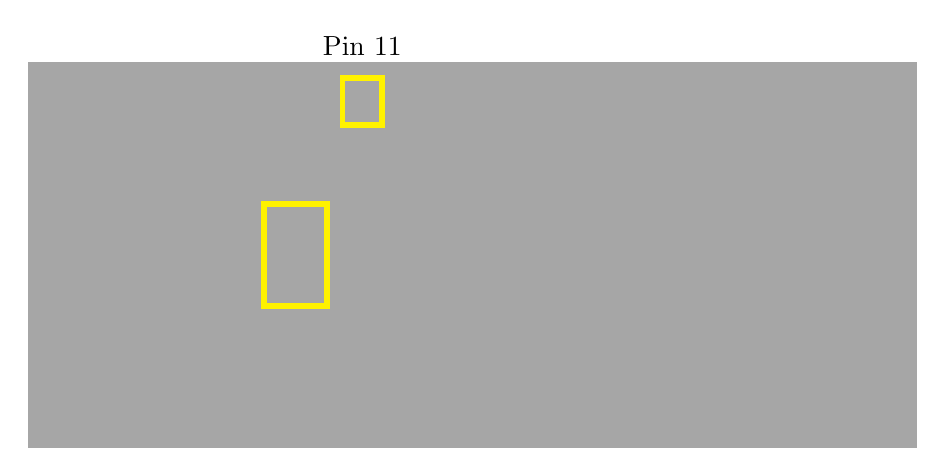
\begin{tikzpicture}
        %\node at (0,0) (Board) {\includegraphics{Arduino/Nano33BLE/Nano33BLESense}};
        
        \ArduinoNanoTikz;
        
        \fill[gray, opacity=0.7] (-11.2,-0.2) rectangle (0.1,4.7);
        
        \coordinate (A) at (-8.2,1.6);
        \coordinate (B) at (-7.4,2.9); 
        
        
        \coordinate (C) at (-7.2,3.9);
        \coordinate (D) at (-6.7,4.5);  
        
        \def\cliparea{(C) rectangle (D); (A) rectangle (B); }  
        
        \begin{scope}
            \clip (A) rectangle (B);
            
            \ArduinoNanoTikz
            
            %\node at (0,0) (Board) {\includegraphics{Arduino/Nano33BLE/Nano33BLESense}};
            
        \end{scope}
        
        %        \fill[ArduinoColor] (C) rectangle (D);
        %         \fill[gray!30] ({-8.16-0.195},4.145) rectangle ++(0.39, 0.39); 
        %        \draw[fill=gray!30,gray!30] (-8.145,4.143) circle(0.195); 
        %        \draw[fill=gray!60,gray!60] (-8.145,4.143) circle(0.165); 
        %        \fill[white,white](-8.145,{4.143+0.39}) circle (0.1275);
        
        \draw[yellow,line width=2pt] (A)  rectangle (B);
        \draw[yellow,line width=2pt] (C)  rectangle (D);
        
        \node (P25) at (-6.95, 4.9) {Pin 11};
    \end{tikzpicture}    
    
    
    
    \captionof{figure}{Arduino Nano 33 BLE Sense's built-in Push Button  with Pin 11}  
\end{center}

}






\section{Specification}

The built-in button is a small white button  and connected to pin 11.\index{Pin!Pin 11}

\begin{description}
    \item [Built-in Button:] \PYTHON{BUTTON\_B =  11u}
\end{description}

If the pin is declared as input in the function \PYTHON{setup}, then it can be used.

%\Mynote{cite data sheet, power consumption?}

The pin 11 must be defined as an input in the function \PYTHON{setup} by setting \PYTHON{pinMode (11, INPUT\_PULLUP)}, otherwise the button cannot be read.

\medskip 


The pin 11 can also be used otherwise. Then the button is not in use. \cite{Arduino:2023a,Arduino:2023,ArduinoNano33Manual:2022}

%\Mynote{What happen if there is another button at the pin? Both in use?}

\Mynote
{
\begin{itemize}
  \item cite data sheet
  \item Circuit Diagram
\end{itemize}
}

\section{Simple Code}


As soon as the button is connected, it can be used. It is not necessary to install a special library. Programming takes place in two steps:

\begin{enumerate}
    \item In the first step, the pin is configured in the function \PYTHON{setup}:
    
    {
        \captionof{code}{Defining the built-in button's pin as an input.}
        \begin{Arduino}
            pinMode(BUTTON_B, INPUT_PULLUP)   
        \end{Arduino}
    }
    \item In the second step, the button can be used in the function \PYTHON{loop}. To read in the value, use the function \PYTHON{digitalRead}:
    
    {
        \captionof{code}{Read the built-in button's state}
        \begin{Arduino}
            buttonState = digitalRead(BUTTON_B);
        \end{Arduino}
    }
    
\end{enumerate}




\section{Tests}


The simplest test is the flashing of an LED for 2 seconds, if the button is pressed, see sketch \ref{Nano:BuiltinButtonTest}.

{
    \captionof{code}{Simple sketch to test the push button and the built-in LED}\label{Nano:BuiltinButtonTest}
    \ArduinoExternal{}{../../Code/Nano33BLESense/PushButton/TestPushButton/TestPushButton.ino}
}

\section{Interrupt Function on the Arduino Nano 33 BLE Sense}


An interrupt is a function that allows the microcontroller on the Arduino Nano 33 BLE Sense to immediately respond to an external event, such as pressing a button, without the need for the program to continuously check for that event. Normally, in a program, the microcontroller would repeatedly check if a button is pressed by running through a loop, which consumes processing power and can slow down other tasks. This is not efficient, especially when the program needs to perform other actions at the same time.

With an interrupt, the program can continue running other tasks, and only when the specified event (like a button press) occurs, the program is temporarily paused to execute a special function known as the \menu{Interrupt Service Routine (ISR)}. The ISR is a small, efficient function designed to handle the event, such as changing a variable or triggering another action. After the ISR is executed, the program returns to where it left off, continuing its normal operation.

Using interrupts in this way helps make the program more efficient and responsive, as it doesn't waste time constantly checking for events and can focus on other tasks until something important happens. This is especially useful for real-time applications where quick responses to external events are necessary, such as in embedded systems, robotics, or sensor monitoring.



\section{Simple Application}



This code sketch \ref{Nano:TestButtonInterrupt} shows how to use an interrupt to control the built-in LED on the Arduino Nano 33 BLE Sense when the built-in push button is pressed.

The program sets up the built-in LED and push button. When the button is pressed, an interrupt runs a special function called an Interrupt Service Routine. The ISR is very short and only sets a flag variable \PYTHON{pushPressed} to \PYTHON{true}, indicating that the button has been pressed.

The main program \PYTHON{loop} checks this flag. If it is set to \PYTHON{true}, the program turns on the LED for 2 seconds, then turns it off and resets the flag to \PYTHON{false}. This ensures the system is ready to detect the next button press. Using the \PYTHON{true and false} values makes it easy to manage the button's state.

This method avoids constantly checking the button’s state, making the program more efficient. Additionally, the Arduino Nano 33 BLE Sense allows all its pins to be used for interrupts. This makes it easy to attach interrupt functions to any pin, allowing quick and efficient responses to inputs like buttons or sensors. \cite{ArduinoInterrupt:2019}


\Mynote{andere Überschrift für simple Application}

\bigskip







{
    \captionof{code}[Simple sketch connects the push button with an interrupt.]{Simple sketch connects the push button with an interrupt. Here, pushing the built-in button is handled by an interrupt. Then the built-in LED switch on for 2 sec.}\label{Nano:TestButtonInterrupt}
    \ArduinoExternal{}{../../Code/Nano33BLESense/PushButton/TestPushButtonInterrupt/TestPushButtonInterrupt.ino}
}

\bigskip

This is just a simple example. The variable \PYTHON{BUTTON\_B} is already defined, so the assignment is not necessary. The command \PYTHON{delay} should be avoided in an Arduino sketch. Instead, variables of the type \PYTHON{elapsedMillis} should be used.



\section{Further Readings}

\begin{itemize}
  \item Boxall, John: \textsl{Arduino Workshop - A Hands-On Introduction with 65 Projects}. No Starch Press, 2021. \cite{Boxall:2021}
  \item Vo{\"s}, Andreas: \textsl{Volumio mit Drehgebern erweitern}. Make Magazin, 2024. \cite{Voss:2024}
  \item K\"uhnel, Claus: \textsl{Arduino - Das umfassende Handbuch}. Rheinwerk Verlag GmbH, 2024. \cite{Kuehnel:2024}
\end{itemize}



  %%%%%%%%%%%%
%
% $Autor: Wings $
% $Datum: 2019-03-05 08:03:15Z $
% $Pfad: TemplateSensor $
% $Version: 4250 $
% !TeX spellcheck = en_GB/de_DE
% !TeX encoding = utf8
% !TeX root = filename 
% !TeX TXS-program:bibliography = txs:///biber
%
%%%%%%%%%%%%

% Structure
\chapter{Pressure and Temperature Sensor LPS22HB}

The sensor LPS22HB is a piezoresistive absolute pressure sensor that is integrated into the Arduino Nano 33 BLE Sense board. It's a digital sensor that measures atmospheric pressure and temperature. The sensor uses a piezoresistive technology to detect changes in pressure. The LPS22HB has an accuracy of $\pm1.5$ hPa and a resolution of 0.01 hPa. It can measure pressures from 260 to 1260 hPa. The sensor also measures temperature with an accuracy of $\pm0.12^\circ$C and a resolution of $0.01^\circ$C. The temperature range is from $-40^\circ$C to $85^\circ$C. 

The LPS22HB communicates with the Arduino board using the protocol I\textsuperscript{2}C. It has a low power consumption of 1.5 $\mu A$ in sleep mode and 1.5 mA in active mode. The sensor is also resistant to shock and vibration. It's a sensor for projects that require accurate pressure and temperature measurements, such as weather stations, altimeters. \cite{Arduino:2023a,Arduino:2023}

Arduino Nano 33 BLE Sense Lite hat  keine HTS221-Temperatur- und Feuchtigkeitssensoren, sondern nur den LPS22HB-Drucksensor, der allerdings auch die Temperatur messen kann

Arduino Nano 33 BLE Sense Rev2 hat  einen HTS221-Temperatur- und Feuchtigkeitssensor und den LPS22HB-Drucksensor, der allerdings auch die Temperatur messen kann.


Unterschiede:

Inertiale Messeinheit (IMU):
Rev 1: Verfügt über eine einzelne 9-Achsen-IMU.
Rev 2: Hat eine Kombination aus zwei IMUs: eine 6-Achsen-IMU (BMI270) und eine 3-Achsen-IMU (BMM150), was die Möglichkeiten zur Bewegungserkennung erweitert1.

Design und Zugänglichkeit:
Rev 2: Integriert neue Pads und Testpunkte für USB, SWDIO und SWCLK, was den Zugang zu diesen wichtigen Punkten auf der Platine erleichtert1.
Rev 1: Hat diese zusätzlichen Pads und Testpunkte nicht.
Stromversorgung:

Rev 2: Verwendet den MP2322 als Stromversorgungskomponente, was die Leistung verbessert1.

Rev 1: Nutzt eine andere Stromversorgungskomponente.
Der Arduino Nano 33 BLE Sense Rev 1 verwendet den MPS MP2144 als Stromversorgungskomponente

\begin{center}    
    
\begin{tikzpicture}
        %\node at (0,0) (Board) {\includegraphics{Arduino/Nano33BLE/Nano33BLESense}};
        
        \ArduinoNanoTikz;
        
        \fill[gray, opacity=0.7] (-11.2,-0.2) rectangle (0.1,4.7);
        
        \coordinate (A) at (-6.55,2.4);
        \coordinate (B) at (-5.9,3.05);    
        
        
        
        \begin{scope}
            \clip (A) rectangle (B);
            
            \ArduinoNanoTikz
            
            %\node at (0,0) (Board) {\includegraphics{Arduino/Nano33BLE/Nano33BLESense}};
            
        \end{scope}
        
        
        \draw[yellow,line width=2pt] (A)  rectangle (B);        
    \end{tikzpicture}    
    
    \captionof{figure}{Arduino Nano 33 BLE Sense's pressure and temperature sensor LPS22HB}  
\end{center}




\section{General}

A pressure sensor is a device that measures the pressure of its surroundings. It works by converting the mechanical energy of the environment into an electrical signal. The sensor typically consists of a diaphragm or membrane, which is a thin, flexible material that changes its shape in response to changes in pressure. The diaphragm or membrane is usually connected to a microcontroller or other electronic device, which reads the electrical signal and converts it into a pressure reading. The pressure sensor can be calibrated to provide accurate readings over a specific pressure range. The sensor can be used in a variety of applications, including industrial control systems, medical devices, and consumer electronics.

Pressure sensors can be classified into two main types: absolute and differential. Absolute pressure sensors measure the absolute pressure of the environment, while differential pressure sensors measure the difference in pressure between two points. Pressure sensors can be used to measure a wide range of pressures, from very low pressures to very high pressures. The accuracy of a pressure sensor depends on its calibration and the quality of its components. Pressure sensors can be affected by various factors, including temperature, humidity, and air flow. Pressure sensors can be used to monitor and control pressure in a variety of applications, including heating and cooling systems, refrigeration systems, and food processing systems. Pressure sensors can be used to detect pressure anomalies and alert users to potential problems. \cite{Gan:2024}

\bigskip

% temperatur
A temperature sensor is a device that measures the temperature of its surroundings. It works by converting the thermal energy of the environment into an electrical signal. The sensor typically consists of a thermistor or thermocouple, which is a device that changes its electrical resistance or voltage in response to changes in temperature. The thermistor or thermocouple is usually connected to a microcontroller or other electronic device, which reads the electrical signal and converts it into a temperature reading. The temperature sensor can be calibrated to provide accurate readings over a specific temperature range. The sensor can be used in a variety of applications, including industrial control systems, medical devices, and consumer electronics.

Temperature sensors can be classified into two main types: contact and non-contact. Contact temperature sensors, such as thermocouples, come into direct contact with the object being measured. Non-contact temperature sensors, such as infrared sensors, do not come into contact with the object being measured.

Temperature sensors can be used to measure a wide range of temperatures, from very low temperatures to very high temperatures. The accuracy of a temperature sensor depends on its calibration and the quality of its components. Temperature sensors can be affected by various factors, including humidity, air flow, and radiation. Temperature sensors can be used to monitor and control temperature in a variety of applications, including heating and cooling systems, refrigeration systems, and food processing systems. Temperature sensors can be used to detect temperature anomalies and alert users to potential problems.



\Mynote{cite books, applications, board}

\section{Specific Sensor}

The pressure sensor of the LPS22HB is a piezoresistive sensor that changes its electrical resistance in response to changes in pressure. The pressure sensor of the LPS22HB is connected to the Arduino Nano 33 BLE Sense, which reads the electrical signal and converts it into a pressure reading. The pressure sensor of the LPS22HB is calibrated to provide accurate readings over a pressure range of 260 to 1260 mbar. The pressure sensor of the LPS22HB is a non-contact sensor, meaning that it does not come into direct contact with the object being measured. The pressure sensor of the LPS22HB is affected by various factors, including temperature and humidity. The pressure sensor of the LPS22HB can be used to monitor and control pressure in a variety of applications, including industrial control systems and consumer electronics. The pressure sensor of the LPS22HB can be used to detect pressure anomalies and alert users to potential problems. The pressure sensor of the LPS22HB has an accuracy of $\pm0.12$ mbar. 

The pressure sensor of the LPS22HB is a low-power sensor, making it suitable for use in battery-powered devices. 

\bigskip
% Temperatur

The LPS22HB is a digital pressure sensor that also includes a temperature sensor. The temperature sensor of the LPS22HB is a thermistor that changes its electrical resistance in response to changes in temperature. The thermistor is connected to the  microcontroller Arduino Nano 33 BLE Sense, which reads the electrical signal and converts it into a temperature reading. The temperature sensor of the LPS22HB is calibrated to provide accurate readings over a temperature range of $-40^\circ$C to $85^\circ$C. The temperature sensor of the LPS22HB is a non-contact sensor, meaning that it does not come into direct contact with the object being measured. 

The temperature sensor of the LPS22HB is affected by various factors, including humidity and air flow. The temperature sensor of the LPS22HB can be used to monitor and control temperature in a variety of applications, including industrial control systems and consumer electronics. The temperature sensor of the LPS22HB can be used to detect temperature anomalies and alert users to potential problems. The temperature sensor of the LPS22HB is a high-accuracy sensor, with an accuracy of $\pm0.12^\circ$C and a resolution of $0.01^\circ$C. 

The temperature sensor of the LPS22HB is a low-power sensor, making it suitable for use in battery-powered devices. 

\Mynote{cite board}

\section{Specification}

The LPS22HB is a digital pressure sensor that measures pressure in the range of 260 to 1260 mbar. It has a high accuracy of $\pm0.12$ mbar and a resolution of 0.01 mbar. The sensor is calibrated to provide accurate readings over a temperature range of $-40^\circ$C to $85^\circ$C. It has a non-contact measurement principle, which means that it does not come into direct contact with the object being measured. The LPS22HB is a compact sensor, measuring $3.5 \times 3.5 \times 1.1$ mm in size. 

It has a low power consumption of $1.5 \mu A$ in active mode and $0.1 \mu A$ in sleep mode.

The sensor has a sampling rate of up to 100 Hz and a data transfer rate of up to 400 kbps. Note that the sampling rate of the sensor LPS22HB can be adjusted using the function \PYTHON{setSamplingRate()} in the Arduino library. The default sampling rate is 100 Hz, but it can be set to 50 Hz, 25 Hz, or 10 Hz using the following code:

\medskip

\PYTHON{lps22hb.setSamplingRate(50); // 50 Hz}

\PYTHON{lps22hb.setSamplingRate(25); // 25 Hz}

\PYTHON{lps22hb.setSamplingRate(10); // 10 Hz}

\medskip


It's worth noting that the sampling rate of the sensor LPS22HB can affect the accuracy and reliability of the measurements. A higher sampling rate can provide more accurate measurements, but it can also increase the power consumption of the sensor.


 The sensor is also resistant to shock, vibration, and temperature changes. It has a high sensitivity and a low noise level, making it suitable for use in applications where high accuracy is required. 



\begin{itemize}
  \item cite data sheet
  \item Circuit Diagram
\end{itemize}

\section{Library}

To program the sensor LPS22HB on the Arduino Nano 33 BLE Sense, you will need to use the library LPS22HB. \cite{ArduinoLPS22HB:2024}

\subsection{Description}

The library LPS22HB is a library for the Arduino platform that provides a simple interface for interacting with the sensor LPS22HB. It allows you to read temperature and pressure values from the sensor, as well as set the sensor's mode and power mode. \cite{ArduinoLPS22HB:2024}


\subsection{Installation}

To use the library LPS22HB, you will need to install it on your Arduino IDE. You can do this by following these steps:

\begin{itemize}
    \item Open the Arduino IDE and navigate to the menu \menu{Sketch}.
    \item Select \menu{Sketch -> Include Library -> Manage Libraries}.
    \item Search for ``LPS22HB'' in the library search bar.
    \item Click on the library ``LPS22HB''  and then click on the buttion ``Install''.
    \item Wait for the library to install and then restart the Arduino IDE.
\end{itemize}

\medskip

Once you have installed the library LPS22HB, you can use it to program the sensor LPS22HB on the Arduino Nano 33 BLE Sense. Here is an example~\ref{LPS22HBSimpleExample} of how you can use the library to read temperature and pressure values from the sensor:

\medskip

{
    \captionof{code}{Example code for the sensor LPS22HB on the Arduino Nano 33 BLE Sense}\label{LPS22HBSimpleExample.ino}
    \ArduinoExternal{}{../../Code/Nano33BLESense/SensorLPS22HB/LPS22HBSimpleExample.ino}
}

\medskip

This sketch \ref{LPS22HBSimpleExample.ino} uses the library LPS22HB to read temperature and pressure values from the sensor LPS22HB and print them to the serial console.

Note that you will need to have the Arduino Nano 33 BLE Sense board connected to your computer and the Arduino IDE installed on your computer in order to use the LPS22HB library.


\subsection{Functions}
Here are the functions of the Arduino library LPS22HB:

\begin{itemize}
  \item Initialization Functions
    \begin{itemize}
      \item \PYTHON{begin()}: Initializes the sensor LPS22HB and sets it up for use.
      \item \PYTHON{reset()}: Resets the sensor LPS22HB to its default state.
    \end{itemize}
  \item Reading Functions
    \begin{itemize}
      \item \PYTHON{readTemperature()}: Reads the temperature value from the sensor LPS22HB.
      \item \PYTHON{readPressure()}: Reads the pressure value from the sensor LPS22HB.
      \item \PYTHON{readAltitude()}: Reads the altitude value from the sensor LPS22HB.
      \item \PYTHON{readTemperatureAndPressure()}: Reads both the temperature and pressure values from the sensor LPS22HB.
    \end{itemize}
  \item Setting Functions
    \begin{itemize}
      \item \PYTHON{setMode()}: Sets the mode of the sensor LPS22HB.
      \item \PYTHON{setPowerMode()}: Sets the power mode of the sensor LPS22HB.
      \item \PYTHON{setSamplingRate()}: Sets the sampling rate of the sensor LPS22HB.
      \item \PYTHON{setFilter()}: Sets the filter of the sensor LPS22HB.
    \end{itemize}
  \item Getting Functions
    \begin{itemize}
      \item \PYTHON{getMode()}: Gets the current mode of the sensor LPS22HB.
      \item \PYTHON{getPowerMode()}: Gets the current power mode of the sensor LPS22HB.
      \item \PYTHON{getSamplingRate()}: Gets the current sampling rate of the sensor LPS22HB.
      \item \PYTHON{getFilter()}: Gets the current filter of the sensor LPS22HB.
    \end{itemize}
  \item Sleep Functions
    \begin{itemize}
      \item \PYTHON{sleep()}: Puts the sensor LPS22HB into sleep mode.
      \item \PYTHON{wakeUp()}: Wakes up the sensor LPS22HB from sleep mode.
    \end{itemize}
  \item Other Functions
    \begin{itemize}
      \item \PYTHON{checkStatus()}: Checks the status of the sensor LPS22HB.
      \item \PYTHON{getError()}: Gets the error code of the sensor LPS22HB.
      \item \PYTHON{resetError()}: Resets the error code of the sensor LPS22HB.
    \end{itemize}
\end{itemize}

\medskip

Note that this list may not be exhaustive, and the library may have additional functions not listed here.

\subsection{Example - Manual}

\subsection{Example}

\subsection{Example - Code}

\subsection{Example - Files}



\section{Calibration}

To calibrate the sensor LPS22HB on the Arduino Nano 33 BLE Sense, you will need to follow these steps. First, upload the calibration code to the Arduino Nano 33 BLE Sense. The calibration code will prompt you to enter the calibration parameters, such as the temperature and pressure values. Enter the calibration parameters, and the code will store them in the sensor's memory. The calibration process will take a few minutes to complete. During the calibration process, the sensor will take multiple readings of the temperature and pressure values. The sensor will then calculate the average of the readings and store it as the calibration value. Once the calibration process is complete, the sensor will be ready to use. To verify the calibration, you can use the calibration code to read the temperature and pressure values from the sensor. Compare the readings with the expected values to ensure that the sensor is calibrated correctly. If the readings are not accurate, you may need to repeat the calibration process. The calibration process can be repeated as many times as necessary to achieve accurate readings. The calibration values can be stored in the sensor's memory and retrieved later. By following these steps, you can calibrate the sensor LPS22HB on the Arduino Nano 33 BLE Sense and ensure accurate readings.

\Mynote{cite method, more mathematics!}




The code \ref{LPS22HBCalibration.ino} reads the temperature and pressure values from the sensor LPS22HB, stores them in the sensor's memory, and prints them to the serial console. The storeCalibration function is used to store the calibration values in the sensor's memory.

\medskip

{
    \captionof{code}{Simple sketch calibrating the sensor LPS22HB}\label{LPS22HBCalibration.ino}
    \ArduinoExternal{}{../../Code/Nano33BLESense/SensorLPS22HB/LPS22HBCalibration.ino}
}

\medskip


Note that this is just an example code and you may need to modify it to suit your specific needs. Additionally, you will need to make sure that the sensor LPS22HB is properly connected to the Arduino Nano 33 BLE Sense and that the I2C interface is enabled.

\section{Simple Code}

\section{Sleep Mode}



{
    \captionof{code}{Sketch for the Arduino Nano 33 BLE Sense to switch the sensor LPS22HB into sleep mode}\label{LPS22HBSleep.ino}
    \ArduinoExternal{}{../../Code/Nano33BLESense/SensorLPS22HB/LPS22HBSleep.ino}
}

\medskip


This sketch \ref{LPS22HBSleep.ino} uses the function \PYTHON{sleep()} to switch the sensor into sleep mode, and the function \PYTHON{wakeUp()} to switch the sensor out of sleep mode. The function \PYTHON{sleep()} puts the sensor into a low-power state, and the function \PYTHON{wakeUp()} restores the sensor to its normal operating state.

Note that the function \PYTHON{sleep()} must be called before the sensor can be put into sleep mode, and the function \PYTHON{wakeUp()} must be called before the sensor can be restored to its normal operating state.

Also, note that the function \PYTHON{sleep()}  can only be called when the sensor is in a valid state, and the function \PYTHON{wakeUp()} can only be called when the sensor is in a valid state.

You can also use the function \PYTHON{setMode()} to set the sensor to sleep mode, and the function \PYTHON{getMode()} to get the current mode of the sensor.

\medskip

\PYTHON{lps22hb.setMode(LPS22HB\_MODE\_SLEEP);}

\PYTHON{lps22hb.getMode();}

\medskip

This will set the sensor to sleep mode and get the current mode of the sensor.

You can also use the function \PYTHON{setPowerMode()}  to set the power mode of the sensor, and the function \PYTHON{getPowerMode()} to get the current power mode of the sensor.

\medskip

\PYTHON{lps22hb.setPowerMode(LPS22HB\_POWER\_MODE\_SLEEP);}

\PYTHON{lps22hb.getPowerMode();}


This will set the power mode of the sensor to sleep mode and get the current power mode of the sensor.

\section{Simple Application}



\section{Tests}

\subsection{Simple Function Test}

\subsection{Test all Functions}

\section{Simple Application}


\section{Further Readings}



 % %%%%%%%%%%%%%%%
%
% $Autor: Wings $
% $Datum: 2020-01-29 07:55:27Z $
% $Pfad: General/SensorAPDS9960.tex
% $Version: 1785 $
%
%
%%%%%%%%%%%%%%%

\chapter{Sensormodul APDS-9960 for Gesture, Proximity, and Color Detection}

The APDS-9960 sensor, integrated on the Arduino Nano 33 BLE Sense, is a multifunctional optical sensor used for gesture recognition, ambient light detection, color sensing, and proximity measurement. The sensor uses an I²C interface for communication and comes equipped with an additional infrared LED.
\cite{Avago:2015}


\begin{center}    
	\begin{tikzpicture}
		\node at (0,0) (Board) {\includegraphics{Arduino/Nano33BLE/Nano33BLESense}};
		
		\fill[gray, opacity=0.7] (-6,-2.4) rectangle (6,2.4);
		
		\coordinate (A) at (-1,0.4);
		\coordinate (B) at (0.2,-0.2);    
		\begin{scope}
			\clip (A) rectangle (B);
			\node at (0,0) (Board) {\includegraphics{Arduino/Nano33BLE/Nano33BLESense}};
		\end{scope}
		\draw[yellow,line width=2pt] (A) rectangle (B);
	\end{tikzpicture}    
	
	\captionof{figure}{Arduino Nano 33 BLE Sense's APDS-9960}
	\label{fig:5.1}
\end{center}

\bigskip


\Mynote{Figure 6.1 must be converted into a TikZ image to maintain consistency}

The sensor is located centrally on the Arduino Nano 33 BLE Sense, as indicated in the Figure \ref{fig:5.1}.










\section{Functionality of the APDS-9960}


The APDS-9960 is a versatile optical sensor that offers multiple functionalities, including color detection, proximity sensing, ambient light measurement, and gesture recognition. Each of these features plays a crucial role in various applications, ranging from smart lighting adjustments to touchless control systems.

In the following sections, each function of the APDS-9960 will be explored in detail, explaining its working principle, the type of data it provides, and its potential use cases.





\section{Key Technical Specifications}
\label{chap:Specification}

\subsection*{Power Supply}
\begin{itemize}
	\item Supply Voltage: 2.4 V to 3.6 V
	\item Maximum Voltage: 3.8 V
\end{itemize}

\subsection*{Power Consumption}
\begin{itemize}
	\item Active ALS Mode (Ambient Light Sensor): 200-250 µA
	\item Proximity and Gesture Modes: 790 µA (without LED)
	\item Sleep Mode: 1-10 µA
\end{itemize}

\subsection*{Temperature}
\begin{itemize}
	\item Operating Temperature Range: -30°C to +85°C
	\item Storage Temperature Range: -40°C to +85°C
\end{itemize}

\subsection*{Optical Properties}
\begin{itemize}
	\item LED Wavelength (max.): 950 nm
	\item LED Drive Current:
	\begin{itemize}
		\item 100 mA (Standard), 50 mA, 25 mA, 12.5 mA
		\item LED Boost Option: 100\%, 150\%, 200\%, 300\% (adjustable current boost)
	\end{itemize}
	\item Max Detection Distance for Color, Proximity and Gesture Sensor 0mm to 100mm
\end{itemize}

\subsection*{Proximity Sensor}
\begin{itemize}
	\item Pulse Width for Proximity Measurement: 4 µs to 32 µs
\end{itemize}

\subsection*{Gesture Sensor}
\begin{itemize}
	\item LED Pulse Count: 1 to 64 pulses
\end{itemize}

\subsection*{Connections}
\begin{itemize}
	\item I²C Communication:
	\begin{itemize}
		\item Data Rates: Up to 400 kHz
		\item Pins:
		\begin{itemize}
			\item SDA (I²C Data)
			\item SCL (I2C Clock)
			\item INT (Interrupt, Open Drain, Active Low)
			\item LDR (LED Driver Input)
		\end{itemize}
	\end{itemize}
\end{itemize}

\subsection*{Dimensions}
\begin{itemize}
	\item Length: 3.94mm
	\item Width: 2.36mm
	\item Height: 1.35mm
\end{itemize}

\cite{Avago:2015}


\section{Library \PYTHON{Arduino\_APDS9960}}

In the case of the APDS-9960 sensor, Arduino provides a library \FILE{Arduino\_APDS9960} for calling functions related to color detection, distance measurement, or gesture recognition.

The library for the sensor is \FILE{Arduino\_APDS9960}. This allows measuring gestures, colors, light intensity, and distances with the sensor. Communication between the Arduino Nano 33 BLE Sense's chip and the APDS-9960 module occurs via an internal I²C interface \cite{Avago:2015}.

The library is included by using the command \PYTHON{\#include <Arduino\_APDS9960.h>}.






\subsection{Installation of APDS-9960 Library}

The library is installed as follows:



\begin{enumerate}
	\item Open the Arduino IDE and navigate to \menu[,]{Tools,Manage Libraries...}.
	\item In the Library Manager, use the search bar to look for "Arduino\_APDS9960".
	\item Several libraries will be displayed. Select the library titled "Arduino\_APDS9960" by Arduino and click \textit{Install}.
	\item Once installed, the IDE will show a message in the console confirming the installation. The "Install" button will also change to "Remove", as seen in Figure \ref{fig:APDS9960}, indicating the library is ready for use.
\end{enumerate}


\begin{center}
	\includegraphics[width=8cm]{Arduino/APDS9960/APDS9960Installed.png}
	\captionof{figure}{APDS-9960 Library Instalation}\label{fig:APDS9960}		
\end{center} 










\subsection{Functions}

After the theoretical overview of the APDS-9960 sensor's functions, the following section will explain the practical implementations. It will demonstrate how the various functions of the sensor, such as color detection, gesture recognition, and proximity sensing, can be applied in practice to activate and evaluate the sensor's capabilities.

\medskip

Here are the codes to utilize the various functions of the APDS-9960 sensor, such as color detection, gesture recognition, and proximity sensing, see \cite{ArduinoAPDS9960:2024}:

\begin{itemize}
	\item \PYTHON{begin()}: The \PYTHON{begin()} method activates and initializes the APDS9960 sensor. It is typically called during the \PYTHON{setup\{\}} phase.
	
	\medskip
	
	\begin{itemize}
		\item Return value \PYTHON{TRUE}: Initialization was successful.
		\item Return value \PYTHON{FALSE}: Initialization failed.
	\end{itemize}
	
	\item \PYTHON{end()}: The \PYTHON{end()} method deactivates the APDS9960 sensor.
	
	
	\item \PYTHON{colorAvailable()}: This method checks if color data is available to be retrieved.
	
	\medskip
	
	\begin{itemize}
		\item Return value \PYTHON{TRUE}: Color data is available.
		\item Return value \PYTHON{FALSE}: No color data is available.
	\end{itemize}
	
	\item \PYTHON{readColor(...)}: This method retrieves the color values from the sensor.
	
	It can either read just the color values or the color values along with the ambient light intensity.
	
	\medskip
	
	To read only the color values:
	
	\PYTHON{int r, g, b;}
	
	\PYTHON{APDS.readColor(r, g, b);}
	
	\medskip
	
	The variables \PYTHON{r}, \PYTHON{g}, and \PYTHON{b} will contain the updated color values. The value range is $0, 1, 2, \ldots, 255$.
	
	\medskip
	
	To read both the color values and ambient light intensity:
	
	\PYTHON{int r, g, b, a;} 
	
	\PYTHON{APDS.readColor(r, g, b, a);}
	
	\medskip
	
	The variables \PYTHON{r}, \PYTHON{g}, and \PYTHON{b} will contain the updated color values, while \PYTHON{a} will contain the ambient light intensity. The value range is $0, 1, 2, \ldots, 255$.
	
	\item \PYTHON{proximityAvailable()}: This method checks if proximity data is available.
	
	\medskip
	
	\begin{itemize}
		\item Return value \PYTHON{TRUE}: Proximity data is available.
		\item Return value \PYTHON{FALSE}: No proximity data is available.
	\end{itemize}
	
	\item \PYTHON{readProximity()}: This method reads the proximity value.
	
	\medskip
	
	\begin{itemize}
		\item Return value \PYTHON{int proximity = APDS.readProximity()}: Returns the proximity value.
		\item Return value \PYTHON{-1}: Proximity could not be determined.
	\end{itemize}
	
	\item \PYTHON{gestureAvailable()}: This method checks if a gesture has been detected.
	
	\medskip
	
	\begin{itemize}
		\item Return value \PYTHON{TRUE}: A gesture has been detected.
		\item Return value \PYTHON{FALSE}: No gesture detected.
	\end{itemize}
	
	\item \PYTHON{setGestureSensitivity()}: Gesture detection is influenced by lighting conditions, speed, and distance of movement. This function allows you to adjust the sensitivity of gesture recognition. A higher value detects more gestures, but increases the chance of false positives. A lower value reduces the likelihood of detecting gestures.
	
	The valid range is \PYTHON{1} to \PYTHON{100}.
	
	The default value is \PYTHON{80}.
	
	\item \PYTHON{readGesture()}: If a gesture has been detected, it can be retrieved using the \PYTHON{readGesture()} method. The possible return values are:
	
	\begin{itemize}
		\item \PYTHON{GESTURE\_UP}: An upward movement has been detected.
		\item \PYTHON{GESTURE\_DOWN}: A downward movement has been detected.
		\item \PYTHON{GESTURE\_LEFT}: A leftward movement has been detected.
		\item \PYTHON{GESTURE\_RIGHT}: A rightward movement has been detected.
		\item \PYTHON{GESTURE\_NONE}: No gesture has been detected.
	\end{itemize}
	
	\item \PYTHON{setInterruptPin()}: This method sets the pin used to trigger a measurement. The pin is usually detected automatically, but can be set manually using this function.
	
	If \PYTHON{-1} is passed, no pin is connected.
	
	If \PYTHON{0} or a higher value is passed, that pin will be used.
	
	The default value depends on the board.
	
	\item \PYTHON{setLEDBoost(...)}: The sensor includes an infrared LED that can be temporarily boosted to provide higher brightness. It can be set to provide up to 300\% of its normal power. This can be configured using this method.
	
	\medskip
	
	Usage:
	
	\begin{itemize}
		\item \PYTHON{0}: Boost to 100\% (default power).
		\item \PYTHON{1}: Boost to 150\%.
		\item \PYTHON{2}: Boost to 200\%.
		\item \PYTHON{3}: Boost to 300\%.
	\end{itemize}    
	
	\medskip
	
	Return values:
	
	\begin{itemize}
		\item \PYTHON{0}: Failure.
		\item \PYTHON{1}: Success.
	\end{itemize}
\end{itemize}




\section{Simple Function Tests}

The following code examples can be used to test and try out all functions of the APDS-9960.

\subsection{Example Color Detection}

The library  \PYTHON{Arduino\_APDS9960} includes an example code demonstrating how to perform color detection with the sensor APDS-9960 on an Arduino Nano 33 BLE Sense. This example also tests the ambient light sensor, as both functionalities rely on the same underlying technology. The measured color channel intensities (Red, Green, and Blue) are displayed in the Serial Monitor for real-time observation.

The sensor APDS-9960 enables accurate RGB color detection by measuring the intensity of red, green, and blue light reflected from an object. These values can be visualized in the Serial Plotter, allowing users to track changes in color intensity over time through a graphical representation. This feature is particularly useful for applications that require real-time color monitoring or dynamic light adjustments.


\subsection{Example Color Detection - Manual}

\Mynote{to do}


\subsection{Setting Up the Color Sensor Measurement Program}

To begin the process of creating the color sensor measurement program, open the Arduino Cloud Editor and navigate to the "Libraries" tab. Search for the "Arduino-APDS9960" library and download it. Afterward, click on "More info" to access the GitHub repository, where several examples are provided.

Next, connect the Arduino Nano 33 BLE Sense to the computer, ensuring that the Cloud Editor detects both the board and the corresponding port. If the board is not automatically recognized, follow the instructions to install the necessary plugin to enable the editor to detect the board. Confirm that the correct port is selected. Finally, upload the program to the Arduino, and by opening the serial monitor, the measured values will be recorded in the Arduino IDE.

\subsection{Example }Color Detection - Code}

First, serial communication is started with \PYTHON{Serial.begin(9600)} to send data to the computer. The command  \PYTHON{APDS.begin()} initializes the sensor and in the event of a potential error, an error message is output via the serial interface.

\bigskip



\bigskip

The code operates within the function \PYTHON{loop()} of a sketch to continuously read and display color values from the APDS-9960 sensor. Initially, it checks if a color reading is available by using the method \PYTHON{APDS.colorAvailable()}. If no reading is available, the program briefly pauses for 5 milliseconds to avoid excessive CPU usage. Once a reading is ready, the method \PYTHON{APDS.readColor(r, g, b)} retrieves the color data and stores the red, green, and blue values in the respective variables. These values are then printed to the Serial Monitor, labeled clearly as ``r'', ``g'', and ``b''. A one-second delay is added before the program repeats the loop, allowing for clear intervals between consecutive readings.




\subsection{Example Color Detection - File}

The program can be found at 

\medskip

{
	\captionof{code}{Simple sketch using the sensor APDS9960 for colors}\label{TestAPDS9960Color}
	\ArduinoExternal{}{../../Code/Nano33BLESense/APDS9960/TestAPDS9960Color/TestAPDS9960Color.ino}
}


\subsection{Proximity}

A simple code for testing the proximity sensor is also provided by the library. The proximity sensor is designed for measuring distances of up to 100mm.

\subsection{Proximity - Manual}

Open the Arduino Cloud Editor and navigate to the Libraries tab. In the search bar, search for the library \PYTHON{Arduino\_APDS9960}. Once located, open the Examples section within the library and select the sketch ``ProximitySensor''.
\smallskip
Connect the Arduino Nano 33 BLE Sense to the computer. Check that the Cloud Editor recognizes the board by verifying if both the board and port are listed in the dropdown menu.

\subsection{Example Proximity - Code}

First, serial communication is started with \PYTHON{Serial.begin(9600)} to send data to the computer. The method \PYTHON{APDS.begin()}  initializes the sensor and in the event of a potential error, an error message is output via the serial interface.


\bigskip


The code operates within the function \PYTHON{loop()}  of a sketch to continuously read and display proximity values from the sensor APDS-9960. It begins by checking if a proximity reading is available using the method \PYTHON{APDS.proximityAvailable()}. If a reading is ready, the method \PYTHON{APDS.readProximity()} retrieves the proximity value, where \PYTHON{0} indicates a close object, \PYTHON{255} indicates a distant object, and \PYTHON{-1} signals an error in reading. This proximity value is then printed to the Serial Monitor. A delay of 100 milliseconds is added before the program repeats the loop, ensuring a brief interval between consecutive readings.


\subsection{Example Proximity - File}

The sketch can be found at 

\bigskip

{
	\captionof{code}{Simple sketch using the sensor APDS9960 for measuring the proximity}\label{TestAPDS9960Proximity}
	\ArduinoExternal{}{../../Code/Nano33BLESense/APDS9960/TestAPDS9960Proximity/TestAPDS9960Proximity.ino}
}

\subsection{Gesture Detection}
\subsection{Example Gesture Detection}

The library \FILE{Arduino\_APDS9960} also provides an example sketch demonstrating gesture detection with the sensor APDS-9960 on an Arduino Nano 33 BLE Sense. Some LED feedback signals have been programmed to provide quick visual feedback.

\subsection{Example Gesture Detection - Manual}

\Mynote{to do}


\subsection{Example Gesture Detection - Code}

In this example sketch, the library \FILE{Arduino\_APDS9960} is integrated first and then the setup is created. In addition, the LED pins are configured so that they behave as outputs.


\bigskip

After that, serial communication is initialized, and the program verifies whether the sensor is correctly initialized using \PYTHON{APDS.begin()}. If initialization fails, an error message is printed. The gesture sensitivity can be adjusted via \PYTHON{APDS.setGestureSensitivity(value)}, where values range from 1 to 100, affecting detection accuracy and sensitivity. The sketch sets a default sensitivity and signals the start of gesture detection by turning off the RGB LEDs with \PYTHON{digitalWrite(LEDR, HIGH)}, \PYTHON{digitalWrite(LEDG, HIGH)}, and \PYTHON{digitalWrite(LEDB, HIGH)}.

In the function \PYTHON{loop()}, the code continuously checks for available gestures using \PYTHON{APDS.gestureAvailable()}. When a gesture is detected, it is read using \PYTHON{APDS.readGesture()} and interpreted within a \PYTHON{switch} statement. Each gesture corresponds to specific LED behavior:

\begin{itemize}
	\item \PYTHON{GESTURE\_UP}: The red LED is briefly turned on, then off after a 1-second delay.
	\item \PYTHON{GESTURE\_DOWN}: The green LED is briefly turned on, then off after a 1-second delay.
	\item \PYTHON{GESTURE\_LEFT}: The blue LED is briefly turned on, then off after a 1-second delay.
	\item \PYTHON{GESTURE\_RIGHT}: All LEDs are turned on simultaneously, then off after a 1-second delay.
\end{itemize}

The \PYTHON{default} case ensures no action if an undefined gesture is detected.



\subsection{Example Gesture Detection - File}

The sketch can be found at 

\bigskip

{
	\captionof{code}{Simple sketch using the sensor APDS9960 for gesture detection}\label{TestAPDS9960Gesture}
	\ArduinoExternal{}{../../Code/Nano33BLESense/APDS9960/TestAPDS9960Gesture/TestAPDS9960Gesture.ino}
}

\subsection{Troubleshoot}


Errors in color detection can be caused by insufficient lighting in the room. Please ensure that the environment is bright enough for the color detection function.


\section{Calibration Color Detection}

\section{Calibration Color Detection}

Due to variations in environmental light conditions and the sensitivity of the sensor, calibration is required to ensure accurate color detection. This section outlines the calibration process using a standard color chart under constant lighting conditions. To carry out the calibration, the Arduino, a connection cable (USB A to USB Micro), and a laptop or computer with the appropriate Arduino development environment are required.

\medskip

The proximity and gesture feature is pre-configured and factory-calibrated to detect proximity and gesture at a distance of 100mm, eliminating the need for customer calibration.
\cite{BroadcomAPDS9960:2024}

\subsection{Calibration Setup}

A standardized color chart is used, which provides reference values for perfect red, green, and blue under constant lighting conditions. The RGB values from the sensor are read as raw, uncalibrated data, which must be normalized to a standard range (0–255) for accurate color detection.\Mynote{citation, picture}

\subsection{Step 1: Measuring Reference Values}

The first step in the calibration process is to measure the raw sensor values for each primary color (red, green, and blue) using the standardized color chart. By placing the color chart in front of the sensor and reading the raw RGB values, we can establish the maximum possible sensor readings for each color channel.

\[
\text{RawRed} = \max(R_{\text{measured}})
\]
\[
\text{RawGreen} = \max(G_{\text{measured}})
\]
\[
\text{RawBlue} = \max(B_{\text{measured}})
\]

These maximum values are obtained by positioning the chart at a fixed distance of one centimeter and ensuring constant light intensity.

\subsection{Step 2: Normalizing the Sensor Values}
Once the maximum sensor readings for red, green, and blue are obtained, the raw sensor data is normalized to a 0-255 scale. This ensures that the sensor's readings correspond to standard RGB values. The following formula is used for normalization:

\[
R_{\text{calibrated}} = \frac{R_{\text{raw}}}{\text{RawRed}} \times 255
\]
\[
G_{\text{calibrated}} = \frac{G_{\text{raw}}}{\text{RawGreen}} \times 255
\]
\[
B_{\text{calibrated}} = \frac{B_{\text{raw}}}{\text{RawBlue}} \times 255
\]

Where:

\begin{itemize}
	\item $R_{\text{raw}}, G_{\text{raw}}, B_{\text{raw}}$ are the raw sensor values for each channel.
	\item $\text{RawRed}, \text{RawGreen}, \text{RawBlue}$ are the maximum measured values from the standard color chart.
\end{itemize}

\subsection{Step 3: Implementing the Calibration in Code}

The normalization process is implemented directly in the Arduino code to adjust the sensor's readings. To begin calibration, open the Serial Monitor, enter ``OK'' in the command line, and press Enter to confirm. The following steps will then be explained through text output.

\bigskip

After the user initiates the calibration by typing ``OK'' into the Serial Monitor, the sketch starts. The sketch guides the user through the calibration of red, green, and blue colors, with each phase confirmed by entering ``OK''. The pins for the RGB LEDs are defined, and variables store the maximum calibration values for each color. Status variables control the sequence, ensuring each phase is completed before moving to the next. These maximum values are later used for accurate color detection in the Application code.

\bigskip


The following code section begins by initializing serial communication at a baud rate of 9600, enabling interaction through the serial monitor. Next, it sets the RGB LED pins as outputs and turns on all LEDs to create white light, which helps capture accurate color measurements. The code then initializes the sensor APDS-9960, checking for successful setup. If the sensor fails to initialize, an error message is printed, and the program halts. If successful, a message confirms initialization and prompts the user to type ``OK'' in the serial monitor to proceed with the calibration process explanation.

\bigskip

The next code segment in the loop first checks if the user has entered ``OK'' to start the calibration process. After confirmation, it displays an explanation and instructions. After showing the explanation, it waits for the user to confirm by typing ``OK'' again, which then initiates the red color calibration by prompting the user to place the red chart in front of the sensor. The loop pauses at each step until the user confirms.

\Mynote{Screen shot?}

\bigskip

Each color calibration starts after the user types ``OK'' in the Serial Monitor. The sketch measures the highest detected value for each color over 10 seconds and sets it as the calibration maximum. After all colors are calibrated, it displays the final maximum values for red, green, and blue in the Serial Monitor, completing the process. The \PYTHON{maxRed}, \PYTHON{maxGreen}, and \PYTHON{maxBlue} values can later be entered into the application sketch to apply the calibration to the sketch.


\subsection{Calibration File}

The sketch can be found at 

\bigskip

{
	\captionof{code}{APDS-9960: Example Calibration}
	\ArduinoExternal{}{../../Code/Nano33BLESense/APDS9960/APDS9960Calibration/APDS9960Calibration.ino}
}


\subsection{Step 4: Validating the Calibration}

To ensure the calibration is successful, the sensor readings should be tested again using the standard color chart. The calibrated values for red, green, and blue should be close to 255 for the respective pure colors on the chart. If the readings deviate significantly, further adjustment of the maximum reference values may be necessary.

\bigskip

The calibration of the sensor APDS-9960 is essential for accurate RGB detection. By using a standard color chart and constant lighting conditions, the sensor's raw values can be normalized to provide consistent and reliable color readings. This process can be further refined by adjusting for specific environmental factors or sensor placement.


\section{Tests}

\subsection{Simple Function Test}

\subsection{Test all Functions}

\section{Simple Application}

Similarly, by following all the steps for uploading and compiling the sketch we can see the results of sensor APDS-9960  on Serial Monitor, too. For seeing the different output, we can change the input for the sensor too, e.g: for color detection we can switch the colors, for gesture detection we can also switch the gestures, and for proximity also do the same. The resulted output as shown in the figure.  \ref{fig:2} 

\Mynote{rewrite and extend}

\begin{center}
	\includegraphics[width=9.5cm]{Nano33BLESense/APDS-Output}
	\captionof{figure}{Gesture, Proximity, Color Sensor Output Window}
	\label{fig:2}
\end{center}

We can also run the single funcnality of this sensor too, e.g; if we just need to capture the color of product, we can also run the color detection program. It depends upon the application and we can implement our application and modify the code as per our desire results.


{
	\captionof{code}{Simple sketch using the sensor APDS9960}\label{TestAPDS9960}
	\ArduinoExternal{}{../../Code/Nano33BLESense/APDS9960/TestAPDS9960/TestAPDS9960.ino}
}




%%%%%%%%%%%%%%%%%%%%%%%%%%%%%%%%%%


\section{Further Readings}

\begin{itemize}
	%    \item S. Grzesik, R. Kluwak, and B. Plikusinski, "Multispectral Sensor Application Possibility Research for Temperature Measurement," \textit{2023 23rd International Conference on Mechatronics - Mechatronika (ME)}, Brno, Czech Republic, pp. 1-6, 2023. Available at: \url{https://ieeexplore.ieee.org/document/10349583}
	
	\item SparkFun Electronics, ``APDS-9960 RGB and Gesture Sensor Hookup Guide''. A comprehensive guide that explains the functionality of the APDS-9960 and provides step-by-step instructions for implementation. Available at: \url{https://learn.sparkfun.com/tutorials/apds-9960-rgb-and-gesture-sensor-hookup-guide/all}, \cite{Hymel:2024}
	
	\item Maker Guides, ``APDS-9960 Gesture and Color Sensor with Arduino''. This tutorial provides a hands-on introduction to using the APDS-9960 sensor with Arduino, including gesture and color recognition. Available at: \url{https://www.makerguides.com/apds-9960-gesture-and-color-sensor-with-arduino/}, \cite{Maetschke:2024}
\end{itemize}




 % %%%%%%%%%%%%
%
% $Autor: Wings $
% $Datum: 2019-03-05 08:03:15Z $
% $Pfad: TemplateSensor $
% $Version: 4250 $
% !TeX spellcheck = en_GB/de_DE
% !TeX encoding = utf8
% !TeX root = filename 
% !TeX TXS-program:bibliography = txs:///biber
%
%%%%%%%%%%%%

% Structure
\chapter{Sensor APDS 9960 Gesture}

Introduction
\Mynote{cite books, applications, board}



\subsection{Sensormodul APDS 9960 for Gesture}


\subsubsection{Function of the Gesture Detection Sensor}

The gesture recognition of the APDS-9960 is based on four additional angled photodiodes

\begin{itemize}
	
	\item Up – Hand movement upwards.
	\item Down – Hand movement downwards.
	\item Left – Hand movement to the left.
	\item Right – Hand movement to the right.
	
\end{itemize}

which detect reflected infrared light (IR) from the integrated IR-LED. By analyzing the reflection, which measures direction-dependent changes using the photodiodes, the sensor can recognize movements and gestures such as swiping motions in different directions (e.g., up, down, left, right). The sensor converts this information into digital data, such as speed, direction, and distance of the movement. The 32-record FIFO register allows the sensor to temporarily store motion data, ensuring continuous processing.
\smallskip
\cite{Avago:2015}


\section{General}

General description

cite books

\section{Specific Sensor}

cite board

\section{Specification}

\begin{itemize}
  \item cite data sheet
  \item Circuit Diagram
\end{itemize}

\section{Bibliothek}

\subsection{Description}

\subsection{Installation}

\subsection{Functions}

\subsection{Example - Manual}

\subsection{Example}

\subsection{Example - Code}

\subsection{Example - Files}



\section{Calibration}

cite method

\section{Simple Code}


\section{Simple Application}



\section{Tests}

\subsection{Simple Function Test}

\subsection{Test all Functions}

\section{Simple Application}


\section{Further Readings}


 % %%%%%%%%%%%%
%
% $Autor: Wings $
% $Datum: 2019-03-05 08:03:15Z $
% $Pfad: TemplateSensor $
% $Version: 4250 $
% !TeX spellcheck = en_GB/de_DE
% !TeX encoding = utf8
% !TeX root = filename 
% !TeX TXS-program:bibliography = txs:///biber
%
%%%%%%%%%%%%

% Structure
\chapter{Sensor APDS 9960 Color}



The general functionality of a color sensor is based on the reflection of white light from the object to be measured. White light contains wavelengths that cover the entire visible spectrum (p. 189 \cite{Rybach:2013}). Due to the molecular structure of the object or chemical processes, such as photosynthesis, certain wavelengths are absorbed while others are reflected. The reflected light rays that reach the color sensor are spectrally selected by color filters or a diffraction grating  \cite{Hering:2023}. 

\section{General}

\textbf{Color filters}: By using parallel red, green, and blue color filters, the intensities of the RGB components are evaluated by three photodiodes behind the filters \cite{Hering:2023}.

\textbf{Diffraction grating}: As light passes through a diffraction grating, the physical diffraction effect occurs. This effect, due to the varying wavelengths of light, produces an interference pattern that enables the spectral decomposition of the light. The spectrum of the incoming light is spatially dispersed, similar to the refraction in a prism (p. 208 ff. \cite{Rybach:2013}). The intensity of the color components can be measured by an array of spatially arranged photodiodes. Diffraction gratings offer higher resolution than color filters \cite{Hering:2023}.

Photodiodes are semiconductors that generate electrical energy through the internal photoelectric effect (p. 220 \cite{Rybach:2013}). The signal from the photodiodes is amplified and stored in a data register through analog-to-digital conversion. The measurement is taken over a specific period. By accumulating the RGB data, the measured color can finally be determined \cite{Avago:2015}. 

Color sensors are typically used in image processing and quality control applications \cite{Avago:2015}.



As shown in Figure \ref{fig:SchematicColorSensor}, the incoming light first passes through UV and IR filters. It is then separated into its red, green, blue, and unfiltered components by color filters. These filtered components are subsequently converted from analog to digital units, as described below.

\begin{center}
	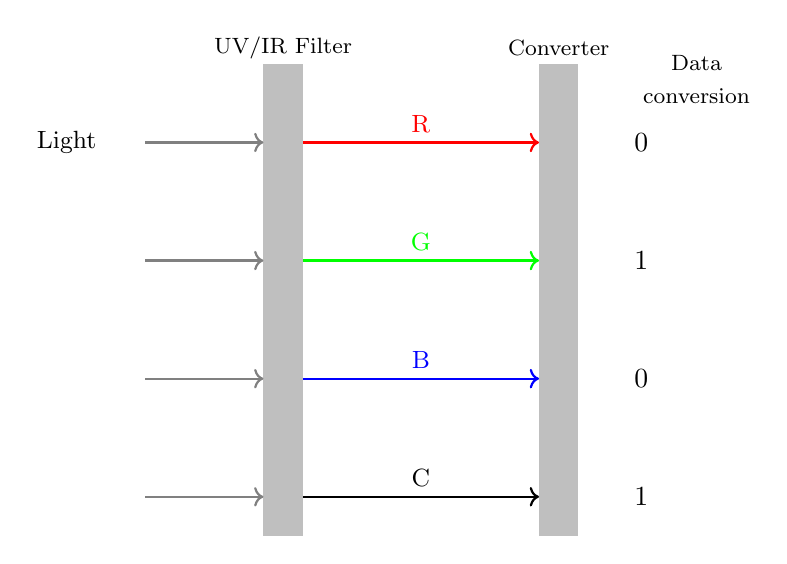
\begin{tikzpicture}
		
		% UV/IR Filter and Converter rectangles
		\fill[gray!50] (2, -2.5) rectangle (2.5, 3.5);
		\fill[gray!50] (5.5, -2.5) rectangle (6, 3.5);
		
		% Labels
		\node at (-0.5, 2.5) {\small Light};
		\node at (2.25, 3.7) {\footnotesize UV/IR Filter};
		\node at (5.75, 3.7) {\footnotesize Converter};
		\node[align=center] at (7.5, 3.3) {\footnotesize Data \\ \footnotesize conversion};
		
		% Arrows for light input
		\draw[->, thick, gray] (0.5, 2.5) -- (2, 2.5);
		\draw[->, thick, gray] (0.5, 1) -- (2, 1);
		\draw[->, thick, gray] (0.5, -0.5) -- (2, -0.5);
		\draw[->, thick, gray] (0.5, -2) -- (2, -2);
		
		% Color-coded arrows
		\draw[->, thick, red] (2.5, 2.5) -- (5.5, 2.5) node[midway, above] {\small R};
		\draw[->, thick, green] (2.5, 1) -- (5.5, 1) node[midway, above] {\small G};
		\draw[->, thick, blue] (2.5, -0.5) -- (5.5, -0.5) node[midway, above] {\small B};
		\draw[->, thick, black] (2.5, -2) -- (5.5, -2) node[midway, above] {\small C};
		
		% Data conversion outputs
		\node at (6.8, 2.5) {0};
		\node at (6.8, 1) {1};
		\node at (6.8, -0.5) {0};
		\node at (6.8, -2) {1};
	\end{tikzpicture}
	
	\captionof{figure}{Schematic of the main function of a color sensor}
	\label{fig:SchematicColorSensor}
\end{center}

The block diagram \ref{fig:FunctionalBlockDiagram} shows the processing flow of the APDS-9660 from light detection to communication via the I²C protocol with the Arduino. The individual steps are explained as follows:

\tikzstyle{block} = [rectangle, draw, minimum width=3.5cm, minimum height=1.2cm, text centered, text width=3.5cm]
\tikzstyle{smallblock} = [rectangle, draw, minimum width=3.5cm, minimum height=1.2cm, text centered]
\tikzstyle{arrow} = [thick,->,>=stealth]
\tikzstyle{sensor} = [draw, isosceles triangle, isosceles triangle apex angle=60, shape border rotate=-90, minimum height=1.5cm, minimum width=1.5cm, text centered]

\begin{center}
	\begin{tikzpicture}[node distance=2.5cm, scale=0.5, every node/.style={transform shape}]
		
		% Sensors
		\node (clear) [sensor] {Clear};
		\node (red) [sensor, below of=clear] {Red};
		\node (green) [sensor, below of=red] {Green};
		\node (blue) [sensor, below of=green] {Blue};
		
		% RGBC + ALS
		\node (rgbc_als) [block, right of=red, xshift=3cm] {RGBC \\ ALS};
		
		% MUX
		\node (mux) [smallblock, right of=rgbc_als, xshift=3cm] {MUX};
		
		% ADC
		\node (adc) [smallblock, right of=mux, xshift=3cm] {ADC};
		
		% FIFO + Threshold Control
		\node (fifo) [block, right of=adc, xshift=3.5cm] {32 x 4 Byte FIFO \\ Threshold Control};
		
		% I2C Interface
		\node (i2c) [block, above of=fifo, yshift=2cm] {I\textsuperscript{2}C Interface};
		
		% Interrupt
		\node (interrupt) [smallblock, below of=fifo, yshift=-2cm] {Interrupt};
		
		% Connections
		\draw [arrow] (clear) -- (rgbc_als);
		\draw [arrow] (red) -- (rgbc_als);
		\draw [arrow] (green) -- (rgbc_als);
		\draw [arrow] (blue) -- (rgbc_als);
		\draw [arrow] (rgbc_als) -- (mux);
		\draw [arrow] (mux) -- (adc);
		\draw [arrow] (adc) -- (fifo);
		\draw [arrow] (fifo) -- (i2c);
		\draw [arrow] (fifo) -- (interrupt);
		\draw [arrow] (i2c) -- ++(2.5cm,0) node[right] {SCL};
		\draw [arrow] (i2c) -- ++(2.5cm,-1.5cm) node[right] {SDA};
		\draw [arrow] (interrupt) -- ++(2.5cm,0) node[right] {INT};
		
	\end{tikzpicture}
	
	\captionof{figure}{Functional Block Diagram}
	\label{fig:FunctionalBlockDiagram}
\end{center}

\Mynote{The graphic is not optimal. Description of the individual blocks is not clear. What does RGBC and ALS mean?}


The photodiodes convert the intensities of the color components of the filtered light and the total light into electrical signals.
These RGBC (Red, Green, Blue, Clear) and ALS (Ambient Light Sensor) signals are forwarded to the next processing stage using the multiplexer (MUX). 

The MUX allows for the sequential processing of the color signals, as the ADC (Analog-to-Digital Converter) can only process one signal at a time.
The ADC converts the analog signal selected by the MUX into a digital value. This conversion is necessary to make the signal suitable for digital processing and transmission.

The digital value is stored in a FIFO (First In, First Out) data register, which can store up to 32 data values (4 bytes each). A threshold controller monitors the data and triggers an interrupt when defined limits are reached. The detailed process is explained in Chapter Data Processing \ref{chap:Data Processing}.

The stored data is transmitted to the Arduino via an I²C bus. The I²C bus uses two lines: the SCL (Serial Clock Line) for the clock and the SDA (Serial Data Line) for data transmission. The detailed functioning of the I²C bus is explained in Chapter \ref{chap:Protokoll I²C} Protokoll I²C.
\cite{Avago:2015}.

\subsubsection{Data Processing}
\label{chap:Data Processing}

The color detection begins at the photodiodes with RGBC detection and ends with 16-bit values stored in the RGBC data registers. The signal from the photodiode array is accumulated over a period defined by the value in the ATIME register (ALS ADC Integration Time) before the results are transferred to the RGBCDATA registers. The gain factor can be set from 1x to 64x, which is controlled via the CONTROL<AGAIN> bit (ALS Gain Control). Performance parameters such as accuracy, resolution, conversion speed, and energy consumption can be adjusted to meet the application requirements.

Between measurements, a customizable, energy-efficient waiting period is maintained, the duration of which is determined by the control bits WEN (Wait Enable), WTIME (Wait Time), and WLONG (Wait Long Enable). The waiting time can range from 0 seconds to a maximum of 8.54 seconds.

An interrupt is triggered when the clear channel values exceed the thresholds defined in the AILTL/AIHTL (ALS low threshold, lower byte/ALS high threshold, lower byte) or AILTH/AIHTH (ALS low threshold, upper byte/ALS high threshold, upper byte) threshold registers. To avoid unwanted or false interrupts, a persistence filter is integrated, ensuring that an interrupt is triggered only when a defined number of consecutive values fall outside the thresholds. This threshold is set in the APERS register (ALS Interrupt Persistence). If a value is within the thresholds, the persistence counter is reset. If the analog circuit is saturated, the ASAT bit is set, indicating potentially inaccurate RGBCDATA results. The AINT (ALS Interrupt) and CPSAT (Clear Diode Saturation) bits can be queried at any time via I²C. However, for AINT to trigger a hardware interrupt on the INT pin, the AIEN bit (ALS Interrupt Enable) must be set. Saturation of the analog-to-digital converter can be detected via the CPSAT bit; to enable this function, the CPSIEN bit (Clear Diode Saturation Interrupt Enable) must be set. The AVALID bit (ALS Valid) is reset by reading the RGBCDATA. ASAT and AINT can be reset via the CICLEAR (Clear Channel Interrupt Clear) or AICLEAR (All Non-Gesture Interrupt Clear) bits.

The RGBC results can be used to determine the color temperature in Kelvin or the ambient light intensity in Lux.

\cite{Avago:2015}








\section{Specific Sensor}

cite board

\section{Specification}

\begin{itemize}
  \item cite data sheet
  \item Circuit Diagram
\end{itemize}

\section{Bibliothek}

\subsection{Description}

\subsection{Installation}

\subsection{Functions}

\subsection{Example - Manual}

\subsection{Example}

\subsection{Example - Code}

\subsection{Example - Files}



\section{Calibration}

cite method

\section{Simple Code}


\section{Simple Application}



\section{Tests}

\subsection{Simple Function Test}

\subsection{Test all Functions}

\section{Simple Application}


\section{Further Readings}


 % %%%%%%%%%%%%
%
% $Autor: Wings $
% $Datum: 2019-03-05 08:03:15Z $
% $Pfad: TemplateSensor $
% $Version: 4250 $
% !TeX spellcheck = en_GB/de_DE
% !TeX encoding = utf8
% !TeX root = filename 
% !TeX TXS-program:bibliography = txs:///biber
%
%%%%%%%%%%%%

% Structure
\chapter{Sensor APDS 9960 Proximity}

The proximity sensor is part of the gesture detection sensor and detects top-bottom gestures based on the temporal change in the measured distance. The proximity detection measures the distance between the sensor and an object by capturing the reflected IR light. The integrated IR LED emits light, which is measured by the same photodiodes as in gesture detection. The stronger the reflection, the closer the object is. The proximity sensor can also detect events such as the approach or withdrawal of an object and trigger corresponding interrupts when predefined thresholds are exceeded. To ensure reliable measurements, the sensor compensates for unwanted reflections by adjusting offset values and suppresses interference from ambient light.
\smallskip
\cite{Avago:2015}



\section{General}

General description

cite books

\section{Specific Sensor}

cite board

\section{Specification}

\begin{itemize}
  \item cite data sheet
  \item Circuit Diagram
\end{itemize}

\section{Bibliothek}

\subsection{Description}

\subsection{Installation}

\subsection{Functions}

\subsection{Example - Manual}

\subsection{Example}

\subsection{Example - Code}

\subsection{Example - Files}



\section{Calibration}

cite method

\section{Simple Code}


\section{Simple Application}



\section{Tests}

\subsection{Simple Function Test}

\subsection{Test all Functions}

\section{Simple Application}


\section{Further Readings}


 % %%%%%%%%%%%%
%
% $Autor: Wings $
% $Datum: 2019-03-05 08:03:15Z $
% $Pfad: TemplateSensor $
% $Version: 4250 $
% !TeX spellcheck = en_GB/de_DE
% !TeX encoding = utf8
% !TeX root = filename 
% !TeX TXS-program:bibliography = txs:///biber
%
%%%%%%%%%%%%

% Structure
\chapter{Sensor Ambient Light}

The ambient light sensor (ALS) of the APDS-9960 works with the same photodiode array and measures the intensity of the ambient light. For this purpose, the UV and IR light filters are installed in front of the photodiodes to ensure accurate measurements of visible light. The sensor converts the measured light intensity into 16-bit data, which enables high resolution and accuracy. A function of programmable gain and customizable integration time ensures that the sensor can operate accurately in different lighting conditions, such as dim or very bright light.
\medskip
Another important feature of the sensor is its ability to correctly detect the intensity of ambient light even behind dark glass, which is particularly useful for devices with tinted covers.
\smallskip
\cite{Avago:2015}


\section{General}

General description

cite books

\section{Specific Sensor}

cite board

\section{Specification}

\begin{itemize}
  \item cite data sheet
  \item Circuit Diagram
\end{itemize}

\section{Bibliothek}

\subsection{Description}

\subsection{Installation}

\subsection{Functions}

\subsection{Example - Manual}

\subsection{Example}

\subsection{Example - Code}

\subsection{Example - Files}



\section{Calibration}

cite method

\section{Simple Code}


\section{Simple Application}



\section{Tests}

\subsection{Simple Function Test}

\subsection{Test all Functions}

\section{Simple Application}


\section{Further Readings}



 % \InputLanguage{Contents/General/}{AppADPS9960}

 % \InputLanguage{Contents/General/}{MicrophoneMP34DT05}

  \InputLanguage{Contents/General/}{IMU}
  \input{../../Contents/General/IMUSoftware}
  \input{../../Contents/General/IMUCalibration}
  \input{../../Contents/General/IMUErrors}
  \input{../../Contents/General/IMULibFunctions}
  %%%
%
% $Autor: Wings $
% $Date: 2024-10-31 11:15:45Z $
% $File: AccelerationDetectionAlgorithms.tex $
% $Version: 1 $
%
%%%


\chapter{Distance,  Speed and Acceleration Detection Algorithms}

\section{Review of Distance Measurement Methods}

Since Mitsubishi released the first cruise control with distance control in 1995, the vast majority of ACC functions have been based on Laser Radar or millimeter-wave radar (MWR). \footnote{MI-PILOT, Mitsubishi Motors, \url{https://www.mitsubishi-motors.com/en/brand/technology/mipilot2/index.html}} But a few have opted to use a binocular camera as the basis for the technology, such as Subaru's EyeSight technology. \footnote{EyeSight technology, Subaru, \url{https://www.subaru.com/eyesight.html}}

Each of these different sets of technical solutions has its own advantages and disadvantages:

\begin{table}[h]
	\centering
	\resizebox{\textwidth}{!}{
		\begin{tabular}{|p{3cm}|p{6cm}|p{6cm}|}
			\hline
			\textbf{Technology} & \textbf{Advantages} & \textbf{Disadvantages} \\ \hline
			\textbf{Laser Radar (LiDAR)} & 
			\begin{tabular}[c]{@{}p{6cm}@{}}
				- High accuracy and resolution \\
				- Capable of creating detailed 3D maps \\
				- Effective for object detection and classification
			\end{tabular} &
			\begin{tabular}[c]{@{}p{6cm}@{}}
				- Expensive \\
				- Affected by adverse weather conditions \\
				- High power consumption
			\end{tabular} \\ \hline
			
			\textbf{Millimeter-Wave Radar} &
			\begin{tabular}[c]{@{}p{6cm}@{}}
				- Less affected by weather conditions \\
				- Long-range detection capabilities \\
				- Lower cost compared to LiDAR
			\end{tabular} &
			\begin{tabular}[c]{@{}p{6cm}@{}}
				- Lower resolution than LiDAR \\
				- Limited in detecting small or non-metallic objects \\
				- Can be affected by interference
			\end{tabular} \\ \hline
			
			\textbf{Binocular Camera Systems} &
			\begin{tabular}[c]{@{}p{6cm}@{}}
				- Lower cost compared to LiDAR and radar \\
				- High resolution for nearby objects \\
				- Uses passive sensing (no emissions)
			\end{tabular} &
			\begin{tabular}[c]{@{}p{6cm}@{}}
				- Computationally intensive \\
				- Accuracy decreases with distance \\
				- Affected by lighting conditions
			\end{tabular} \\ \hline
		\end{tabular}
	}
	\caption{Comparison of distance measurement technologies: LiDAR, Millimeter-Wave Radar, and Binocular Cameras}
	\label{tab:comparison}
\end{table}

For cars using Laser Radar, LiDAR operates by emitting laser pulses towards objects in front of the vehicle. When these pulses hit an object, they are reflected back to the sensor, which measures the time it takes for the pulses to return. This time-of-flight measurement allows the system to calculate the precise distance to the object, as well as its relative speed and position. For cars using millimeter-wave radar, the functional implementation is similar.

For systems that use binocular cameras, this process can be relatively more complex; essentially distance recognition for binocular camera-based systems utilizes bionics: Binocular disparity. This method involves using a pair of cameras positioned at a certain distance apart to capture two images with different viewing angles. By comparing the disparity between the two images (i.e., the difference in pixel positions).\footnote{Mansour, M., Davidson, P., Stepanov, O. and Piché, R., 2019. Relative Importance of Binocular Disparity and Motion Parallax for Depth Estimation: A Computer Vision Approach. Remote Sensing, 11(17), p.1990. \url{https://doi.org/10.3390/rs11171990}}

\begin{equation}
	\text{depth} = \frac{f \times \text{baseline}}{\text{disparity}}
\end{equation}

where depth represents the distance of an object from the camera, f denotes the focal length of the camera, baseline is the distance between the two cameras, and disparity is the difference in image location of the object in the two camera views.

\begin{figure}[H]
	\centering
	\begin{minipage}{1\textwidth}
		\centering
		\includegraphics[width= 0.75\linewidth]{AccelerationDetectionAlgorithms/Baseline.png}
		\caption{Design of OAK-D Pro camera}
	\end{minipage}
\end{figure}

For the OAK-D Pro camera, the baseline distance, which is the distance between the two monochrome cameras, is 7.5 cm. \footnote{OAK-D Pro Camera Documentation, Luxonis, 2021}

According to OAK's official documentation\footnote{OAK China official Website, OAK China, 2024}, the OAK-D Pro can reach a theoretical maximum of 35m, but at this distance there is a very significant margin of error (about 33\% of the theoretical error\footnote{Depth range enhancement, Luxonis Community, 2022}) where the distance fluctuates very significantly. However, there are ways to improve the accuracy of distance detection, such as half-pixel mode to improve the accuracy of distance detection, and averaging distances over a period of time to calculate relative distances to improve the accuracy of relative speed calculations.


\section{Review of Speed and Acceleration Detection Algorithms}

For the measurement of relative velocity, the three schemes mentioned above will actually have two different principles and calculations.

Millimeter-wave radar primarily calculates the relative speed of objects using the Doppler effect. When the radar signal hits a moving object, the frequency of the reflected wave changes depending on the relative speed between the radar and the object. This frequency shift (Doppler shift) is directly proportional to the relative speed of the object. \footnote{Millimeter Wave Radar Sensors: Fundamentals, Texas Instruments, 2018}

For LiDAR and Binocular Camera Systems, the relative speed of objects is calculated based on the change in distance over time. By continuously measuring the distance to an object and comparing it with previous measurements.

Each of these different sets of technical solutions has its own advantages and disadvantages:

\begin{table}[h]
	\centering
	\resizebox{\textwidth}{!}{
		\begin{tabular}{|p{3cm}|p{6cm}|p{6cm}|}
			\hline
			\textbf{Technology} & \textbf{Advantages} & \textbf{Disadvantages} \\ \hline
			\textbf{Laser Radar (LiDAR)} & 
			\begin{tabular}[c]{@{}p{6cm}@{}}
				- High accuracy and resolution \\
				- Capable of creating detailed 3D maps \\
				- Effective for object detection and classification
			\end{tabular} &
			\begin{tabular}[c]{@{}p{6cm}@{}}
				- Expensive \\
				- Affected by adverse weather conditions \\
				- High power consumption
			\end{tabular} \\ \hline
			
			\textbf{Millimeter-Wave Radar} &
			\begin{tabular}[c]{@{}p{6cm}@{}}
				- Less affected by weather conditions \\
				- Long-range detection capabilities \\
				- Lower cost compared to LiDAR
			\end{tabular} &
			\begin{tabular}[c]{@{}p{6cm}@{}}
				- Lower resolution than LiDAR \\
				- Limited in detecting small or non-metallic objects \\
				- Can be affected by interference
			\end{tabular} \\ \hline
			
			\textbf{Binocular Camera Systems} &
			\begin{tabular}[c]{@{}p{6cm}@{}}
				- Lower cost compared to LiDAR and radar \\
				- High resolution for nearby objects \\
				- Uses passive sensing (no emissions)
			\end{tabular} &
			\begin{tabular}[c]{@{}p{6cm}@{}}
				- Computationally intensive \\
				- Accuracy decreases with distance \\
				- Affected by lighting conditions
			\end{tabular} \\ \hline
		\end{tabular}
	}
	\caption{Comparison of distance measurement technologies: LiDAR, Millimeter-Wave Radar, and Binocular Cameras}
	\label{tab:comparison}
\end{table}




}


%\Ausblenden
{

\part{Arduino Nano 33 BLE Sense - External  Sensors and Actors}

  \input{../../Contents/Nano33BLESense/TinyMLKit}

  %%%%%%%%%%%%%%%
%
% $Autor: Wings $
% $Datum: 2020-01-29 07:55:27Z $
% $Pfad: General/PowerTinyMLShield.tex
% $Version: 1785 $
%
%
%%%%%%%%%%%%%%%

%source: https://projecthub.arduino.cc/paulsb/temp-and-humidity-monitor-with-graphs-and-battery-monitor-cd011a

% https://www.az-delivery.de/products/az-delivery-laderegler-tp4056-mini-usb?variant=12239811084384
%https://www.az-delivery.de/products/cd60l-batterieladecontroller
%https://www.az-delivery.de/products/mini-solarpanel?variant=39475872792672

    
\chapter{Powering the TinyML Shield}

Now that you have your Arduino development board up and running, let's talk about how you could deploy it independent of your computer! While some embedded systems call on AC-DC converters (or “wall warts,” colloquially) to provide low voltage power to their electronics (the Google home speaker, for example), others are battery powered. Both of these paradigms are applicable to real-world deployment of tinyML and both are achievable using your TinyML kit.

\Mynote{Komplettes Kapitel muss überarbeitet werden. Sortierung, Quellen, Diagramm,\ldots}
\subsection{USB Power Delivery}

To this point, we have provided power over USB to our microcontroller via the microB port on the Nano 33 BLE Sense. The 5V that USB carries is then down regulated on the development board to 3.3V, the logical reference for the MCU. While there’s nothing wrong with this in development, a prototype of your application ought not depend on drawing power from your computer. Instead, you could call on an AC-DC converter with USB output. This has the added benefit of likely raising the current capacity of the 5V power rail, from at most 500 mA via a computer to whatever the specification happens to be for a given wall-bound converter. This could be meaningful for driving certain power hungry actuators, like speakers.

\section{Battery}

While the above solution removes the need for the computer, you’re still tethered to a wall. To go fully mobile you’ll want to call on a battery. So what are our options? The idea of using a voltage regulator (specifically, the MPM3610) to cut down an input voltage to a nice, stable 3.3V level applies here as well. If you were to take a closer look at the linked datasheet, you’d find that the MPM3610 accepts input voltages from 4.5V to 21V. The 5V delivered over USB is within this range, and any compatible battery will need to be as well. This unfortunately eliminates the possibility of calling on single cell 3.7V lithium batteries, but makes the selection of a 9V alkaline battery fairly obvious.

You might be wondering how any battery might connect to the boards in front of you, but never fear, we’ve got you covered. At one corner of the Tiny Machine Learning Shield you’ll find a green terminal block with silkscreen labels that read, “VIN” and “GND,” where GND is our reference voltage and as such should be connected to the negative terminal of any compatible battery. This green terminal block is where you’d want to screw in wires carrying 4.5V to 21V, and we’ll add that 9V clip, like this, that terminates in pre-stripped hook-up wire makes this quite easy!

\bigskip

Assembly Steps

\begin{enumerate}
    \item Screw down a wire leading from the negative battery terminal (black) to GND (Most < 3mm flat-head screwdrivers will suffice here).
    \item Repeat this process for the positive battery terminal (red) to VIN. And that's it you're all set to power your Arduino from a battery!
\end{enumerate}


\bigskip

Important Notes

\begin{enumerate}
    \item While there is clever circuitry on board to handle such an exception, it is generally good practice to avoid having competing power sources, so we’d recommend that you unplug the Nano 33 BLE Sense from USB power before connecting a battery
    
    \item With about 550 mAh capacity, a 9V battery can source 15 mA for about 37 hours before you will need to get a new one.
\end{enumerate}


\Mynote{tikz-Bild des Shields fehlt.}

\medskip

\begin{center}
  \includegraphics[width=\textwidth]{Battery/batteryScrew.png}
  \captionof{figure}{Montage des Clips}
\end{center}


An image of screwing down the black negative terminal to attach a wire.

\begin{center}
  \includegraphics[width=\textwidth]{Battery/batteryDone.png}
  \captionof{figure}{Komplettes System mit Batterie}
\end{center}

An image of the attached battery powering the device.


\section{Checking the Battery Voltage}

We use an analog input pin to read the voltage. As we are running from a 3.7V volt battery, we need to adjust the reference voltage used by the pin as otherwise it would be comparing the voltage to itself. The statement \PYTHON{analogReference(INTERNAL)} sets the pin to compare the input voltage to a regulated 1.1V. We therefore need to reduce the voltage on the input pin to less than 1.1V for this to work. This is done by dividing the voltage using 2 resistors, 1m and 330k ohms. This divides the voltage by approximately 4 so when the battery is fully charged, which is 4.2V, the voltage at the pin input is 4.2/4 = 1.05V. 

\begin{lstlisting}[language=python]
// Battery Monitor
#define MONITOR_PIN  A0              // Pin used to monitor supply voltage
const float voltageDivider  = 4.0;   // Used to calculate the actual voltage fRom the monitor pin reading
                                     // Using 1m and 330k ohm resistors divids the  voltage by approx 4
                                     // You may wany to substitute  actual values of resistors in an equation (R1 + R2)/R2
                                     // E.g. (1000 + 330)/330 = 4.03
                                     // Alternatively  take the voltage reading across the battery and from the joint between 
                                     //  the 2 resistors to ground and divide one by the other to get the value.
    
// Read the monitor pin and calculate the voltage 
float BatteryVoltage()
{ 
    float reading = analogRead(MONITOR_PIN); 
    // Calculate voltage - reference voltage is 1.1v 
    return 1.1 * (reading/1023) * voltageDivider; 
} 
\end{lstlisting}

The function \PYTHON{BatterVoltage()}, reads the analog pin, which will range from 0 for 0V to 1,023 for 1.1V and using this reading calculates the actual voltage coming form the battery. 

The function \PYTHON{DrawScreenSave()} function calls this then selects the appropriate bitmap to display based on the following: 

\begin{itemize}
    \item If voltage is greater then 3.6V - full 
    \item Voltage between 3.5 and 3.6V - 3/4 
    \item Voltage between 3.4 and 3.5V - half 
    \item Voltage between 3.3 and 3.4V - 1/4 
    \item Voltage < 3.3V - empty 
\end{itemize}



\section{Batterieclip}

Der Batterieclip in Abb. \ref{Batterieclip für 9-Volt-Block}, der vom Hersteller \textit{reichelt} ist, kann vertikal an einen 9-Volt-Block angeschlossen werden. Die dazugehörigen Anschlussdrähte haben eine Länge von 150 mm. Der Anschlussclip ist in der I-Form ausgeführt, weshalb er sich platzsparend ins Gehäuse einbinden lässt \cite{Reichelt:2011}.

\begin{figure}[h]
    \begin{center}
        \includegraphics[width=3in]{Battery/clip.jpg}
        \caption{Batterieclip für 9-Volt-Block\cite{Reichelt:2024a}}
        \label{Batterieclip für 9-Volt-Block}
    \end{center}
\end{figure} 



\section{Spannungssensor}

Der Spannungssensor in Abb. \ref{Spannungssensor} von dem Hersteller \textit{Shenzhen Global Technology Co., Ltd} kann bei der Versorgungsspannung von 3,3 V Spannungen in dem Bereich von 0 V bis 16,5 V messen. Dieser wird genutzt, um den Ladestand der Batterie zu überwachen. Die analoge Auflösung des Sensors liegt bei 10 Bit. Damit kann bei dem angegebenen Messbereich die Spannung mit der Auflösung von 0,016 V gemessen werden. Zur Eingangsschnittstelle gehört der \ac{vcc}-Anschluss und der \ac{gnd}-Anschluss \cite{Shenzhen:2015}. Die Bauteilmaße betragen 13 mm x 27 mm.



{\begin{center}
		
  \includegraphics[width=0.6\textwidth]{Battery/VoltageSensor}
  
  \captionof{figure}{Voltage Sensor 170640  von dem Hersteller \textit{Shenzhen Global Technology Co., Ltd}\cite{Shenzhen:2015}}   		
		
	\end{center}
}
	
Mit dem Sketch \FILE{TestBattery.ino}, siehe \ref~{TestBattery}, soll der Spannungssensor getestet werden.

\medskip



\begin{code}
	
	\caption{Beispiel-Sketch zum Testen der Batterie}\label{TestBattery}

    \ArduinoExternal{}{../../Code/Arduino/Battery/TestBattery.ino}
\end{code}

\subsection{Durchführung}

Für den Test werden die folgenden Hardware-Komponenten benötigt:

\begin{itemize}
    \item Arduino Nano 33 BLE Sense Lite
    \item Tiny Machine Learning Shield
    \item USB-A auf USB-Mikro Verbindungskabel
    \item Grove Jumper zu Grove 4 Pin Kabel
    \item Spannungssensor
    \item Batterie
    \item Batterieclip
\end{itemize}

Die Hardware-Komponenten werden  zusammengebaut, aber die Batterie wird noch nicht angeschlossen. Dann wird der Arduino Nano 33 BLE Sense Lite mit einem Computer verbunden. Anschließend wird der Sketch \FILE{TestBattery.ino} auf den Arduino Nano 33 BLE Sense Lite geladen und der serielle Monitor in der Arduino \acs{ide} geöffnet. Die Batterie wird während des Tests an den Batterieclip angeschlossen und der gemessene Wert bei dem seriellen Monitor ausgelesen.

\subsection{Ergebnisse}

Zu Beginn des Tests zeigt der serielle Monitor die Spannung 0 V an. Nach dem Anschließen der Batterie an den Spannungssensor wird die Spannung 9,6 V angezeigt.  Abbildung~\ref{BildSpannungTest} zeigt den gemessenen Spannungsverlauf. Die angezeigte Spannung liegt in dem erwarteten Bereich einer 9 V Batterie.

\begin{figure}[h]
    \begin{center}
        \includegraphics[width=\textwidth]{Battery/BatteryTest.png}
        \caption{Testoutput des Spannungssensors}
        \label{BildSpannungTest}
    \end{center}
\end{figure}



  %%%%%%%%%%%%
%
% $Autor: Wings $
% $Datum: 2019-03-05 08:03:15Z $
% $Pfad: PushButton $
% $Version: 4250 $
% !TeX spellcheck = en_GB/de_DE
% !TeX encoding = utf8
% !TeX root = filename 
% !TeX TXS-program:bibliography = txs:///biber
%
%%%%%%%%%%%%

% Structure
\chapter{TinyML Shield: Built-in Push Button}\index{Push Button! Built-in Push Button}

\section{General}

A push button is a simple switch mechanism used to control various devices and processes. It is typically made of hard materials like plastic or metal.
The surface of a push button is designed to be easily depressed or pushed by the human finger or hand. When you press a push button, it either closes or opens an electrical circuit. 

In industrial and commercial applications, push buttons can be linked together so that pressing one button releases another. Emergency stop buttons, often with large mushroom-shaped heads, enhance safety in machines and equipment. Pilot lights are sometimes added to push buttons to draw attention and provide feedback when the button is pressed. Color-coding is common to associate push buttons with their specific functions (e.g., red for stopping, green for starting). \cite{DIN:13850}

%\Mynote{cite books, applications, board\\ image of the board}






\section{Built-in Push Button}

The Arduino Nano 33 BLE Sense features an onboard push button. This button is a simple electrical switch that can be activated by pressing it. When you press the button, it completes an electrical circuit. The push button is designed for user interaction and can be used for various purposes.

The built-in button \PYTHON{BUTTON\_B} is connected with pin 11.\index{Pin!Pin 11} Using the function \PYTHON{pinMode(BUTTON\_PIN, INPUT\_PULLUP)} the pin is declared as an input. As can be seen in the sketch, pressing the button can be used to trigger actions; typical actions include switching on an LED, changing modes, or initiating sensor readings.
Overall, the push button provides a convenient way to interact with the Arduino Nano 33 BLE Sense and create responsive projects. \cite{Arduino:2023a,Arduino:2023,ArduinoNano33Manual:2022}


\bigskip


\Mynote{Push Button hier nochmal mit tikz-code hervorheben}

\begin{center}
	
	\begin{tikzpicture}
		\ArduinoNanoShieldTikz
	\end{tikzpicture}    
	
	%  \includegraphics[width=0.9\textwidth]{Nano33BLESense/TinyMLKit/TinyMachineLearningShieldRotated.png}
	\captionof{figure}[The Tiny Machine Learning Shield]{ Tiny Machine Learning Shield \cite{ArduinoShield:2021}}
\end{center}






\Ausblenden{arg1


\begin{center}    
    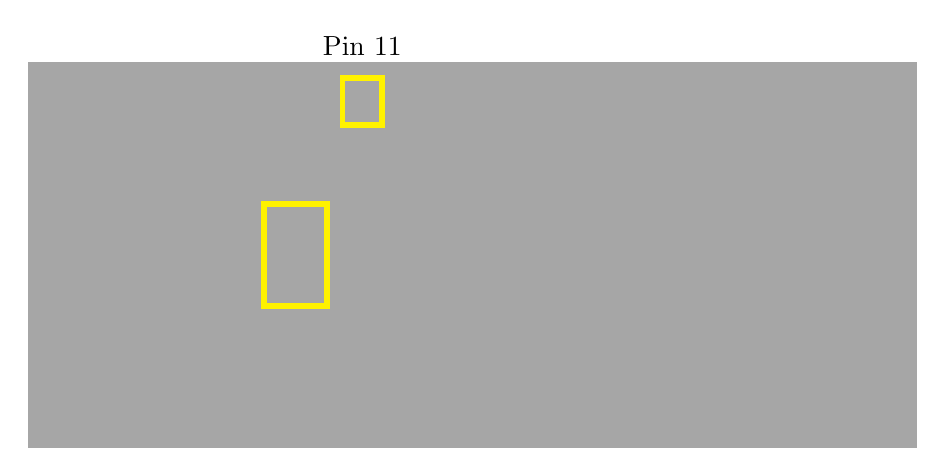
\begin{tikzpicture}
        %\node at (0,0) (Board) {\includegraphics{Arduino/Nano33BLE/Nano33BLESense}};
        
        \ArduinoNanoTikz;
        
        \fill[gray, opacity=0.7] (-11.2,-0.2) rectangle (0.1,4.7);
        
        \coordinate (A) at (-8.2,1.6);
        \coordinate (B) at (-7.4,2.9); 
        
        
        \coordinate (C) at (-7.2,3.9);
        \coordinate (D) at (-6.7,4.5);  
        
        \def\cliparea{(C) rectangle (D); (A) rectangle (B); }  
        
        \begin{scope}
            \clip (A) rectangle (B);
            
            \ArduinoNanoTikz
            
            %\node at (0,0) (Board) {\includegraphics{Arduino/Nano33BLE/Nano33BLESense}};
            
        \end{scope}
        
        %        \fill[ArduinoColor] (C) rectangle (D);
        %         \fill[gray!30] ({-8.16-0.195},4.145) rectangle ++(0.39, 0.39); 
        %        \draw[fill=gray!30,gray!30] (-8.145,4.143) circle(0.195); 
        %        \draw[fill=gray!60,gray!60] (-8.145,4.143) circle(0.165); 
        %        \fill[white,white](-8.145,{4.143+0.39}) circle (0.1275);
        
        \draw[yellow,line width=2pt] (A)  rectangle (B);
        \draw[yellow,line width=2pt] (C)  rectangle (D);
        
        \node (P25) at (-6.95, 4.9) {Pin 11};
    \end{tikzpicture}    
    
    
    
    \captionof{figure}{Arduino Nano 33 BLE Sense's built-in Push Button  with Pin 11}  
\end{center}

}






\section{Specification}

The built-in button is a small white button  and connected to pin 11.\index{Pin!Pin 11}

\begin{description}
    \item [Built-in Button:] \PYTHON{BUTTON\_B =  11u}
\end{description}

If the pin is declared as input in the function \PYTHON{setup}, then it can be used.

%\Mynote{cite data sheet, power consumption?}

The pin 11 must be defined as an input in the function \PYTHON{setup} by setting \PYTHON{pinMode (11, INPUT\_PULLUP)}, otherwise the button cannot be read.

\medskip 


The pin 11 can also be used otherwise. Then the button is not in use. \cite{Arduino:2023a,Arduino:2023,ArduinoNano33Manual:2022}

%\Mynote{What happen if there is another button at the pin? Both in use?}

\Mynote
{
\begin{itemize}
  \item cite data sheet
  \item Circuit Diagram
\end{itemize}
}

\section{Simple Code}


As soon as the button is connected, it can be used. It is not necessary to install a special library. Programming takes place in two steps:

\begin{enumerate}
    \item In the first step, the pin is configured in the function \PYTHON{setup}:
    
    {
        \captionof{code}{Defining the built-in button's pin as an input.}
        \begin{Arduino}
            pinMode(BUTTON_B, INPUT_PULLUP)   
        \end{Arduino}
    }
    \item In the second step, the button can be used in the function \PYTHON{loop}. To read in the value, use the function \PYTHON{digitalRead}:
    
    {
        \captionof{code}{Read the built-in button's state}
        \begin{Arduino}
            buttonState = digitalRead(BUTTON_B);
        \end{Arduino}
    }
    
\end{enumerate}




\section{Tests}


The simplest test is the flashing of an LED for 2 seconds, if the button is pressed, see sketch \ref{Nano:BuiltinButtonTest}.

{
    \captionof{code}{Simple sketch to test the push button and the built-in LED}\label{Nano:BuiltinButtonTest}
    \ArduinoExternal{}{../../Code/Nano33BLESense/PushButton/TestPushButton/TestPushButton.ino}
}

\section{Interrupt Function on the Arduino Nano 33 BLE Sense}


An interrupt is a function that allows the microcontroller on the Arduino Nano 33 BLE Sense to immediately respond to an external event, such as pressing a button, without the need for the program to continuously check for that event. Normally, in a program, the microcontroller would repeatedly check if a button is pressed by running through a loop, which consumes processing power and can slow down other tasks. This is not efficient, especially when the program needs to perform other actions at the same time.

With an interrupt, the program can continue running other tasks, and only when the specified event (like a button press) occurs, the program is temporarily paused to execute a special function known as the \menu{Interrupt Service Routine (ISR)}. The ISR is a small, efficient function designed to handle the event, such as changing a variable or triggering another action. After the ISR is executed, the program returns to where it left off, continuing its normal operation.

Using interrupts in this way helps make the program more efficient and responsive, as it doesn't waste time constantly checking for events and can focus on other tasks until something important happens. This is especially useful for real-time applications where quick responses to external events are necessary, such as in embedded systems, robotics, or sensor monitoring.



\section{Simple Application}



This code sketch \ref{Nano:TestButtonInterrupt} shows how to use an interrupt to control the built-in LED on the Arduino Nano 33 BLE Sense when the built-in push button is pressed.

The program sets up the built-in LED and push button. When the button is pressed, an interrupt runs a special function called an Interrupt Service Routine. The ISR is very short and only sets a flag variable \PYTHON{pushPressed} to \PYTHON{true}, indicating that the button has been pressed.

The main program \PYTHON{loop} checks this flag. If it is set to \PYTHON{true}, the program turns on the LED for 2 seconds, then turns it off and resets the flag to \PYTHON{false}. This ensures the system is ready to detect the next button press. Using the \PYTHON{true and false} values makes it easy to manage the button's state.

This method avoids constantly checking the button’s state, making the program more efficient. Additionally, the Arduino Nano 33 BLE Sense allows all its pins to be used for interrupts. This makes it easy to attach interrupt functions to any pin, allowing quick and efficient responses to inputs like buttons or sensors. \cite{ArduinoInterrupt:2019}


\Mynote{andere Überschrift für simple Application}

\bigskip







{
    \captionof{code}[Simple sketch connects the push button with an interrupt.]{Simple sketch connects the push button with an interrupt. Here, pushing the built-in button is handled by an interrupt. Then the built-in LED switch on for 2 sec.}\label{Nano:TestButtonInterrupt}
    \ArduinoExternal{}{../../Code/Nano33BLESense/PushButton/TestPushButtonInterrupt/TestPushButtonInterrupt.ino}
}

\bigskip

This is just a simple example. The variable \PYTHON{BUTTON\_B} is already defined, so the assignment is not necessary. The command \PYTHON{delay} should be avoided in an Arduino sketch. Instead, variables of the type \PYTHON{elapsedMillis} should be used.



\section{Further Readings}

\begin{itemize}
  \item Boxall, John: \textsl{Arduino Workshop - A Hands-On Introduction with 65 Projects}. No Starch Press, 2021. \cite{Boxall:2021}
  \item Vo{\"s}, Andreas: \textsl{Volumio mit Drehgebern erweitern}. Make Magazin, 2024. \cite{Voss:2024}
  \item K\"uhnel, Claus: \textsl{Arduino - Das umfassende Handbuch}. Rheinwerk Verlag GmbH, 2024. \cite{Kuehnel:2024}
\end{itemize}



 % %%%
%
% $Autor: Wings $
% $Datum: 2021-05-14 $
% $Pfad: GitLab/MLEdgeComputer $
% $Dateiname:  JSTConnector
% $Version: 4620 $
%
% !TeX spellcheck = de_DE/GB
% !TeX program = pdflatex
% !BIB program = biber/bibtex
% !TeX encoding = utf8
%
%%%

\chapter{Connectors of Type JST}

% https://en.wikipedia.org/wiki/JST_connector

\section{Connector Series}

JST connectors are electrical connectors manufactured to the design standards originally developed by J.S.T. Mfg. Co. (Japan Solderless Terminal).\cite{JST:2016} JST manufactures numerous series (families) and pitches (pin-to-pin distance) of connectors.


JST manufactures a large number of series (families) of connectors. The PCB (wire-to-board) connectors are available in top (vertical) or side (horizontal) entry, and through-hole or surface-mount. \cite{JST:2020}

This description refers exclusively to the mechanical structure and electrical behaviour. The pin assignment is not standardised.

Attention: The term ``JST'' is sometimes incorrectly used as a vernacular term meaning any small white electrical connector mounted on \ac{pcb}s.




\section{JST VH}

%\URL{https://www.jst-mfg.com/product/index.php?series=262}

The technical data of the JST VH series is given in this section. They are taken from the data sheet for the series. \cite{JST:2021}

\subsection{Product Profile}


\begin{tabular}{ll}
  Series   & VH connector \\
  Category & Crimp Style Connectors (Wire-to-Board type) \\
  Type     & Crimp style, Compact type, \\
           & With locking device\\
           & Disconnectable type \\
  Feature  & With secure locking device\\
\end{tabular}

\subsection{Specification}

\begin{tabular}{ll}
  Pitch          & 3.96mm \\
  Pin rows       & 1 \\
  Current rating & 10A (AWG\#16) \\
  Voltage rating & 250V\\
  PC board mounting direction & Top entry, Side entry  
\end{tabular}  


\begin{center}
    \includegraphics[width=0.6\textwidth]{JSTConnectors/JSTVH}
    \captionof{figure}{JST connector type VH \URL{https://www.jst-mfg.com/product/index.php?series=262}
    }
\end{center}


\section{JST PH}

The technical data of the JST PH series is given in this section. They are taken from the data sheet for the series. \cite{JST:2022}
%https://www.jst-mfg.com/product/index.php?series=199

\subsection{Product Profile}

\begin{tabular}{ll}
  Series   & PH connector \\
  Category & Crimp Style Connectors (Wire-to-Board type)\\
  Type     & Crimp style, Thin type \\
           & Disconnectable type \\
\end{tabular}

\subsection{Specification}

\begin{tabular}{ll}
  Pitch  & 2.0mm  \\
  Current rating & 2A (AWG\#24) \\
  Voltage rating & 100V \\
  PC board mounting direction & Top entry, Side entry \\
\end{tabular}

\begin{center}
    \includegraphics[width=0.6\textwidth]{JSTConnectors/JSTPH}
    \captionof{figure}{JST connector type VH \cite{JST:2022}} 
\end{center}

\subsection{JST PHR-2}

One variant of the connector series is the JST PHR-2 type, which has 2 pins. Figure \ref{JST-2022} shows a JST PHR-2 connector.

\begin{center}
    \includegraphics[width=0.6\textwidth]{JSTConnectors/PHR-2.jpg}
    \captionof{figure}{JST connector type PHR-2 \cite{JST:2022}}\label{JST-2022}
\end{center}



%  \input{../../Contents/General/Grove}

%  \input{../../Contents/General/ButtonGrove}

 % \input{../../Contents/General/LEDExternal}

%  \input{../../Contents/General/LEDRGBExternal}

%  \input{../../Contents/General/SensorBME280}

 % \input{../../Contents/General/ServoDrive}

  \input{../../Contents/General/OLED}

%  \InputLanguage{Contents/General/}{CAMov2640} 

%  \input{../../Contents/General/CAMov7675}
  
%  %%%
%
% $Autor: Wings $
% $Datum: 2021-05-14 $
% $Pfad: GitLab/MLEdgeComputer/Contents/General/LensCalibrationTool $
% $Dateiname: LensCalibrationTool
% $Version: 4620 $
%
% !TeX spellcheck = de_DE/GB
%
%%%



\chapter{Lens Calibration Tool}


\section{Circle Grid Camera Calibration Patterns}

You can download a PDF version of the circle grid calibration pattern that our SceneScan stereo vision sensor uses for camera calibration. This pattern is compatible to the OpenCV asymmetric circle grid, and can thus also be used for other purposes.
    
When printing the pattern, please ensure that your PDF viewer or printer driver do not scale the document. Otherwise you will not be able to receive accurate metric measurements through stereo vision. You can verify that your printed pattern has the correct scaling, by measuring the reference line at the top of each document.

\begin{figure}
    \begin{center}
        \includegraphics[scale=0.15]{Camera/pattern-a4.pdf}
        
        \caption{Circle Grid Camera Calibration Patterns}
    \end{center}    
\end{figure}

\section{Siemens Star}

The siemens star enables the exact focusing of camera lenses. That is why we print it on the back of our calibration boards. In order to make the camera focusing easier for you as well, you can download our siemens star here.


\begin{figure}
    \begin{center}
        \includegraphics[scale=0.1]{Camera/siemens-star.pdf}
        
        \caption{Siemens Star}
    \end{center}    
\end{figure}

\section{Enjoyyourcamera Testkarte für Kameras und Objektive 30 $\times$ 45 cm}

Testen Sie Ihre Objektive jetzt selbst! Entwickelt vom Tierfotografen Benny Rebel (Bekannt aus Film \& Fernsehen), 400dpi Druck. Testbereiche für Schärfe, Auflösung, Kontrast, Chromatische Abberation, Fokus. Nahtlos erweiterbar für größere Test-Fläche.

Mehrere Testkarten zu einer großen Testkarte zusammenfügbar
Eine Testkarte für Normal- und Teleobjektive, ab 4 Testkarten für Weitwinkelobjektive
Festes Papier, hohe Druckqualität, extrem feine Detailelemente
Einfache Bedienung, Lieferung im stabilen Karton
Sehr viele Testkriterien in einer Karte vereint.


\begin{figure}
    \begin{center}
        \includegraphics[scale=0.1]{Camera/CalibrateCard}
        
        \caption{Siemens Star}
    \end{center}    
\end{figure}

\subsection{Testkarte zum Prüfen von Kameras und Objektiven in Bezug auf ihre Qualität und mögliche Defekte}

Mithilfe dieser von dem Naturfotografen Benny Rebel entwickelten Testkarte lassen sich Kameras und Objektive relativ unkompliziert hinsichtlich ihrer Qualität und möglicher Defekte testen. Damit bietet die Testkarte eine preisgünstige Möglichkeit, die eigene Ausrüstung individuell zu prüfen, und das unabhängig von Testberichten, die wegen einer hohen Serienstreuung bei einigen Objektiv- und Kameramarken oft nicht repräsentativ sind.

\subsection{Zahlreiche Testkriterien: z.B. Schärfe in der Mitte und an den Bildränder, Randabschattungen u.v.m.}

Die Karte deckt zahlreiche Testkriterien ab. Die Kriterien für Kameras sind zum Beispiel die Schärfe in der Bildmitte und an den Rändern, die Auflösung, die Farbwiedergabe, den Kontrastumfang, den Weißabgleich, den Moiré-Effekt, eventuelle Probleme beim automatischen Scharfstellen und das Bildrauschen bei unterschiedlichen ISO-Einstellungen testen. Die Testkriterien für Objektive sind unter anderem Schärfe, Auflösung, Kontrast, Brillanz, Farbwiedergabe, Randabschattungen, chromatische Aberration, Verzeichnung, Vignettierung, eventuelle Probleme beim automatischen Scharfstellen, eine mögliche Dezentrierung der Linsenelemente sowie die Beugung bei unterschiedlichen Blenden.

\subsection{Mehrere Testkarten zu einer großen Testkarte zusammenfügbar - ideal für Weitwinkelobjektive}

Die Testkarte ist so konzipiert, dass man vier oder neun identische Testkarten zu einer großen Testkarte zusammenfügen kann. Für diesen Zweck sind die Testelemente an den Rändern und in den Ecken der Testkarte derart abgeschnitten, dass sie auf einer benachbarten Karte nahtlos weiterverlaufen. Eine große Testfläche, wie sie durch das Zusammenfügen mehrerer Testkarten entsteht, ist wichtig zum Prüfen von weitwinkeligen Objektiven. Solche Objektive besitzen von Natur aus einen weiten Bildwinkel und demzufolge auch einen sehr großen Bildausschnitt. Mit einer großen Testkarte ist sichergestellt, dass die Testfläche den gesamten Bildausschnitt des jeweiligen Objektivs abdeckt, damit man selbst in den Bildecken die Schärfe und andere Kriterien prüfen kann.

\subsection{Eine Testkarte für Normal- und Teleobjektive, vier Testkarten für Weitwinkelobjektive usw.}

Für Normal- und Teleobjektive genügt eine einzelne Testkarte, für Objektive mit einer Brennweite zwischen 50mm und 24mm sollte man vier Testkarten verwenden, und für stark weitwinkelige Objektive mit einer Brennweite von weniger als 24mm empfiehlt sich die Benutzung von 9 Testkarten. Zum Testen von Superweitwinkelobjektiven mit einer Brennweite von weniger als 16mm ergibt es sogar Sinn, die Testkarten nicht direkt aneinanderzufügen. Stattdessen sollte man einen Abstand zwischen den Karten lassen. Wichtig: Die obengenannten Brennweiten beziehen sich auf Objektivtests an Vollformatkameras. Bei Objektivtests an Crop-Kameras verändern sich die Grenzen entsprechend dem Formatfaktor der Kamera. Während man zum Beispiel für ein 35mm-Objektiv an einer Vollformatkamera vier Testkarten benötigt, braucht man für das gleiche 35mm-Objektiv an einer Crop-Kamera mit einem Formatfaktor von 1,5 nur eine Testkarte, denn 35mm x 1,5 ist gleich 52,5mm. Prinzipiell gilt aber: Je größer die Testfläche, desto besser sind die Testergebnisse. Es ergibt also durchaus Sinn, auch zum Testen eines Normalobjektivs vier Testkarten zu verwenden.

\subsection{Festes Papier, hohe Druckqualität, extrem feine Detailelemente für besonders genaues Testen}

Die Testkarte ist auf ein sehr festes, stabiles Papier gedruckt. Außerdem ist die Karte mit einer Druckqualität von 400 dpi extrem detailreich. Die feinsten Detailelemente sind sogar nur einen Punkt breit. Das ermöglicht ein ganz besonders genaues Testen von Objektiv- und Kameraeigenschaften. Außerdem befinden sich die wesentlichen Testflächen sowohl in der Mitte der Karte als auch an den Rändern und in den Ecken. So kann man Eigenschaften wie zum Beispiel die Schärfequalität im gesamten Bildbereich testen. Das hilft dabei, selbst subtile Mängel wie einen Schärfeabfall in den Ecken aufzuspüren.

\subsection{Handhabung}

\begin{enumerate}
  \item Bringen Sie die Testkarte(n) an einer senkrechten, geraden Fläche an. Dafür eignen sich zum Beispiel Holzplatten, gerade Wände oder Glasscheiben. Stellen Sie sicher, dass die Karte gleichmäßig beleuchtet wird, und dass auf der Karte keine Reflexionen zu sehen sind.

  \item Stellen Sie sicher, dass sich die Objektivachse in einem 90 Grad Winkel zur Vorderseite der Testkarte(n) befindet. Richten Sie die Kamera so aus, dass der Bildausschnitt exakt die Testkarte(n) abdeckt. Das Zentrum der Objektivachse sollte genau auf den Mittelpunkt der Testkarte(n) gerichtet sein.

  \item Um ein unverfälschtes Ergebnis zu bekommen, muss die Kamera absolut vibrationsfrei ausgelöst werden. Je nach Brennweite können schon geringe Abweichungen eine Randunschärfe auf dem Foto erzeugen. Benutzen Sie deshalb am besten ein Stativ und einen Fernauslöser. Aktivieren Sie außerdem, sofern vorhanden, die Spiegelvorauslösung. Und deaktieren Sie die Bildstabilisierung.

  \item Für einen Standardtest empfehlen sich folgende Einstellungen:Stellen Sie die Kamera auf Blendenvorwahl (Zeitautomatik) und die Lichtempfindlichkeit auf ISO 200. Wählen Sie idealerweise das Bildformat RAW. Arbeiten Sie außerdem mit dem manuellen Weißabgleich, nach dem Sie diesen auf das Umgebungslicht abgestimmt haben. Für weiterführende Tests, wie zum Beispiel das Bildrauschen bei verschiedenen ISO-Einstellungen, können Sie Einstellungen an der Kamera verändern.

  \item endenreihen: Als erstes Bild bietet sich immer die Offenblende an. Danach kann man der Reihe nach alle Blendenschritte testen (z.B. 1.0 - 1.4 - 2.0 - 2.8 - 4.0 - 5.6, 8.0 - 11 - 16 - 22).

  \item Brennweitenreihen bei Zoom-Objektiven: Auf jeden Fall sollten Sie die Anfangsbrennweite und die Endbrennweite testen. Bei einem 24-70mm Objektiv wären das die Brennweiten 24mm und 70mm. Danach können Sie die Brennweiten in den Schritten testen, wie Sie auch als Festbrennweiten häufig genutzt werden: Das hat den den Vorteil, dass man dann die Abbildungsleistung des jeweiligen Objektivs auch mit der Qualität gängiger Festbrennweiten vergleichen kann.

  \item Und ganz wichtig: Um beim Testen von Wechselobjektiven und Wechselobjektivkameras feststellen zu können, ob ein Defekt vom Objektiv oder von der Kamera ausgeht, sollten Sie Objektive an verschiedenen Kameras testen, und Kameras mit verschiedenen Objektiven. Defekte und Qualitätsmängel müssen nicht zwingend vom Objektiv ausgehen, auch ein schief in der Kamera verbauter Chip kann eine Ursache für eine mangelnde Bildqualität sein.
\end{enumerate}


\bigskip

\section{B.I.G. RES7 Testtafel für Kameras und Objektive}

Die RES7 Testtafel, in der Größe 32x47cm mit matter Oberfläche, wurde für Fotografen entwickelt, um die Bildqualität zu testen und die Grenzen der Auflösung von Kamera und Objektiv beurteilen zu können.

Mit der Tafel kann die Messung der Bildqualität von Digitalkameras, die Messung der Auflösung von optischen Geräten (Vergrößerung 30-50x), die Kontrolle der Belichtung, die grobe Bestimmung gering auflösender Objektive (5-10x) sowie die Kontrolle der Fokussierung und der Schärfentiefe durchgeführt werden.

Die Testtafel eignet sich für Fotokameras bis zu 4000 aktiven Pixeln in der Bildhöhe, d.h. für alle Kompakt-, sowie DSLR- oder DSLM-Kameras mit einer maximalen Auflösung von 24 Megapixeln.

\begin{figure}
    \begin{center}
        \includegraphics[width=0.8\textwidth]{Camera/Testtafel}
        
        \caption{Siemens Star}
    \end{center}    
\end{figure}

\subsection{BIG RES7 Test Board für Kameras und Objektive}
Das BIG RES7 Test Board für Kameras und Objektive in der Größe 32 x 47 cm mit einer matten Oberfläche wurde für Fotografen entwickelt, um die Bildqualität zu testen und die Grenzen der Kamera- und Objektivauflösung abzuschätzen.

Das Board kann zur Messung der Bildqualität von Digitalkameras, zur Messung der Auflösung optischer Geräte (30-50-fache Vergrößerung), zur Kontrolle der Belichtung, zur groben Bestimmung niedrig auflösender Objektive (5-10-fach) und zur Kontrolle von Fokus und Schärfentiefe verwendet werden.

\subsection{Merkmale des BIG RES7 Test Boards für Kameras und Objektive}

\begin{itemize}
  \item Entwickelt für Fotografen zum Testen der Bildqualität
  \item Um die Grenzen der Kamera- und Objektivauflösung abzuschätzen
  \item Um die Bildqualität von Digitalkameras zu messen
  \item Um die Auflösung von optischen Geräten zu messen (Vergrößerung 30-50x)
  \item Matte Oberfläche
  \item Abmessungen: 32 x 47 cm
\end{itemize}


\section{Pattern Generator}

\URL{https://calib.io/pages/camera-calibration-pattern-generator}

\URL{https://markhedleyjones.com/projects/calibration-checkerboard-collection}



Customize a pattern to match your application perfectly and download a printable PDF file. The pattern generator and its outputs can be used for internal development or educational use only. Any commercial purposes or re-sale is strictly prohibited without prior consent. 

NOTE: When printing on a standard inkjet or laser printer, please make sure that your software or printer does not apply any scaling to the pattern. Also make sure that no rasterisation is performed in the printer driver. It is advisable to measure the final pattern after printing.

Once you have settled on a pattern and would like to order a professionally made, highly accurate calibration target, feel free to send us an email at sales@calib.io , and we will happily give you a quote!


\begin{figure}
    \begin{center}
        \includegraphics[width=0.8\textwidth]{Camera/calib.io_charuco_200x150_8x11_15_11_DICT_4X4.pdf}
        
        \caption{Siemens Star}
    \end{center}    
\end{figure}


\begin{figure}
    \begin{center}
        \includegraphics[width=0.8\textwidth]{Camera/calib.io_checker_200x150_8x11_15.pdf}
        
        \caption{Siemens Star}
    \end{center}    
\end{figure}


\section{Chess Board}

\cite{Ntouskos:2007}
\cite{Ntouskos:2007a}
\cite{Ntouskos:2009}
\cite{Prokos:2012}

\begin{figure}
    \begin{center}
        \includegraphics[width=0.8\textwidth]{Camera/camera-calibration-checker-board_9x7.pdf}
        
        \caption{Siemens Star}
    \end{center}    
\end{figure}






\section{To Do}

Arducam Lens Calibration Tool, Sichtfeld (Field of View, FoV) Test Chart Folding Card, Pack of 2

\url{https://www.amazon.com/-/de/dp/B0872Q1RLD/ref=sr_1_40?__mk_de_DE=ÅMÅŽÕÑ&dchild=1&keywords=arducam&qid=1622358908&sr=8-40}

\begin{description}
  \item[Multifunktional für Objektiv:] Objektivfokus kalibrieren, FoV messen und Schärfe abschätzen
  \item[Einfach zu bedienen:] Schnelle Einrichtung in Sekunden und Messung in Minuten mit Online-Videotutorial.
  \item[Ein handliches Werkzeug:] Einfaches Ermitteln des Sichtfelds des Objektivs ohne Berechnung
  \item[Sauber und aufgeräumt:] Faltbarer Kartenstil, mehrfach gefaltet und aufgerollt für schnelle Einstellung und bessere Lagerung
  \item[Anwendung:] Fokuskalibrierung, Schärfeschätzung und Bildfeld-Schnellmessung für M12, CS-Mount, C-Mount und DSLR-Objektive.

\end{description}
\url{https://www.arducam.com/product/arducam-lens-calibration-tool-field-of-view-fov-test-chart-folding-card-pack-of-2/}


\begin{figure}
  \begin{center}
    \includegraphics[width=\textwidth]{CAM/LensCalibrationTool/LensCalibrationTool}
    \quad 
    \includegraphics[width=\textwidth]{CAM/LensCalibrationTool/LensCalibrationTool4}
  
    \caption{Kalibrierungswerkzeug der Firma Arducam; \cite{Arducam:2021}}
  \end{center}    
\end{figure}

\section{Übersicht}

Sind Sie immer noch frustriert von der Berechnung des FOV Ihrer Objektive und den unscharfen Bildern? Arducam hat jetzt ein multifunktionales Tool für Objektive veröffentlicht, mit dem Sie das Sichtfeld des Objektivs ohne Berechnung erhalten und den Objektivfokus schnell und einfach kalibrieren können.

\section{Applications}

Focus calibration, sharpness estimation and field of view quick measuring for M12, CS-Mount, C-Mount, and DSLR lenses

\section{Package Contents}

2*Foldable Lens Calibration Card


\subsection{Licht, Farben und Farbmodelle}
{Farbe ist eine Eigenschaft des Lichts, die durch die verschiedenen Wellenlängen des sichtbaren Lichtspektrums entsteht. Farben werden durch das menschliche Auge wahrgenommen, wenn Licht auf Objekte trifft und reflektiert wird. Diese reflektierten Lichtwellen werden von den Photorezeptoren (Zapfen) in der Netzhaut des Auges erfasst und vom Gehirn interpretiert. \cite{Hasche:2016}
    
 Es gibt in der Programmierung verschiedene Farbmodelle, die je nach Anwendungsbereich verwendet werden. Die wichtigsten Farbmodelle sind:}

\subsubsection{Das additive RGB-Farbmodell (Rot, Grün, Blau)}

Die Farben bei dem Farbmodell RGB werden mittels der Farbmischung von Rot, Grün und Blau zusammengesetzt. Mittels dieser drei Grundfarben können verschiedene Kombinationen und damit unterschiedliche Farben erzeugen werden. Mischt man alle Grundfarben, erhält man weiß. Schaltet man alle Grundfarben ab, so erhält man Schwarz.
    Die Grundfarben können Werte zwischen 0 und 255 einnehmen, wodurch die Helligkeit dieser Grundfarbe eingestellt werden kann. \cite{Hasche:2016}

\begin{itemize}
    \item Beispiel: RGB (255, 0, 0) repräsentiert die Farbe Rot.
\end{itemize}



\subsubsection{Das HSV Farbmodel}
{HSV (Hue, Saturation, Value): Ein Farbmodell, das Farben in Bezug auf Farbton, Sättigung und Helligkeit beschreibt. Dieses Modell ist besonders nützlich in der Bildbearbeitung und bei der Farbauswahl, da es eine intuitive Darstellung der Farbkomponenten bietet.
    
    Hue (Farbton): Bestimmt die Grundfarbe und wird in Grad von 0 bis 360 angegeben.\\
    
    Saturation (Sättigung): Bestimmt die Intensität der Farbe und wird als Prozent-\\wert von 0\% (Grau) bis 100\% (voll gesättigte Farbe) dargestellt.\\
    
    Value (Helligkeit): Bestimmt die Helligkeit der Farbe und wird ebenfalls als Prozent-\\wert von 0\% (schwarz) bis 100\% (volle Helligkeit) dargestellt. \cite{Hasche:2016}
    \\
    \textbf{Beispiel:}
}

\begin{itemize}
    \item Hue (Farbton): 0°
    \item Saturation (Sättigung): 50\%
    \item Value (Helligkeit): 100\%  \\
    \\
    Diese Werte beschreiben ein helles Rot im HSV-Farbmodell.
\end{itemize}

\subsubsection{Graustufen}
{Graustufenerkennung bezieht sich auf die Verarbeitung von Bildern, die keine Farbinformationen enthalten, sondern nur Helligkeitswerte. Ein Graustufenbild ist ein Bild, bei dem jeder Pixel einen Helligkeitswert hat, der typischerweise in einem Bereich von 0 (schwarz) bis 255 (weiß) liegt.
    
    Umwandlung von Farbbildern in Graustufenbilder.\\
    
    Farbbilder können in Graustufenbilder umgewandelt werden, indem die Farbkanäle (Rot, Grün und Blau) kombiniert werden, um einen einzelnen Helligkeitswert zu erzeugen. 
    Eine Möglichkeit ist das Umwandeln mit der Durchschnittsmethode, bei dem der  Graustufenwert durch den Durchschnitt der RGB-Werte berechnet wird.
}

\begin{equation}
    Gray = \frac{ R + G + B }{ 3}
\end{equation}

{Um die Wahrnehmungsempfindlichkeit des menschlichen Auges auf Farben zu berücksichtigen, kann folgende Formel verwendet werden:
}

\begin{equation}
    Gray = 0.33 \times R + 0.22\times G+ 0.17\times B
\end{equation}

Dieses Verfahren liefert in der Regel bessere Ergebnisse, da es die menschliche Wahrnehmung besser widerspiegelt. \cite{Hasche:2016}

\newpage
\subsection{Texterkennung}
{Grundsätzlich funktioniert Texterkennung über das sogenannte ``Optical character recognition'' (OCR), hierfür müssen aber erstmal einige Voraussetzungen getroffen werden.}

\subsubsection{Voraussetzungen}
{Das Bild muss begradigt werden, dies kann hier aber vernachlässigt werden, wenn man davon ausgeht, dass die Kamera vorher in der Testumgebung kalibriert wurde.
    \\
    Zudem muss das Bild ggf. in ein binäres schwarz-weiß-Bild umgewandelt werden.
}

\subsubsection{Identifizieren der Buchstabenmatrix}
{Es werden zuerst die einzelnen Zeilen identifiziert, indem nach zwei durchgehenden Reihen weißer Pixel in X-Richtung gesucht wird, zwischen welchen schwarze und weiße Pixel gemischt sind, wie in Abbildung \ref{fig:Zeilenerkennung} zu sehen ist.
}

\begin{figure}
    \centering
    \includegraphics[width=0.5\linewidth]{LensCalibrationTool/LineRecognition.png}
    \caption{Zeilenerkennung}
    \label{fig:Zeilenerkennung}
\end{figure}

{Analog dazu werden auch die einzelnen Buchstaben identifiziert, indem nach zwei, durchgehend weißen Reihen in Y-Richtung gesucht wird, zwischen welchen schwarze und weiße Pixel gemischt sind.
}
\\
{Dann werden die einzelnen Buchstaben in eine binäre Matrix übertragen (siehe Abbildung \ref{fig:Buchstaben in binäre Matrix umwandeln}), um sie im nächsten Schritt analysieren zu können.
}

\begin{figure}
    \centering
    \includegraphics[width=0.5\linewidth]{LensCalibrationTool/LettersInBinaryMatrix.png}
    \caption{Buchstaben in binäre Matrix umwandeln}
    \label{fig:Buchstaben in binäre Matrix umwandeln}
\end{figure}

\subsubsection{Zuordnung der Buchstaben durch Sektionierung}
{Der Mittelpunkt der Buchstabenmatrix wird mithilfe folgender Formel errechnet.}

\begin{equation}
    d\equiv\sqrt{ \left( Y_{2  } -Y_{1}\right)^2+\left(X_{2  } -X_{1}  \right)^2 })     
\end{equation}

Mithilfe des Mittelpunkts wird die Buchstabenmatrix in mehrere kleine Sektionen geteilt, um sie besser analysieren zu können. 


Eine mögliche Unterteilung in Sektionen ist in Abbildung \ref{fig:Sektionierung der Buchstabenmatrix} zu sehen.

\begin{figure}
    \centering
    \includegraphics[width=0.5\linewidth]{LensCalibrationTool/SectioningTheLetterMatrix.png}
    \caption{Sektionierung der Buchstabenmatrix}
    \label{fig:Sektionierung der Buchstabenmatrix}
\end{figure}

{Nun werden die einzelnen Sektionen mit der gleichen Sektion sämtlicher Buchstaben, aus sämtlichen Schriftarten verglichen und dem Buchstaben zugeordnet, der die größte statistische Übereinstimmung hat.
}
\\
\subsubsection{Einfacherer Prozess der Zuordnung}
{Um den Prozess zu vereinfachen, lässt sich die Buchstabenmatrix auch in Quadranten teilen, anstatt der vielen Sektionen, wie in Abbildung \ref{fig:Unterteilung der Buchstabenmatrix in Quadranten} zu sehen.
}

\begin{figure}
    \centering
    \includegraphics[width=0.5\linewidth]{LensCalibrationTool/DivisionOfTheLetterMatrixIntoFourQuadrants.png}
    \caption{Unterteilung der Buchstabenmatrix in Quadranten}
    \label{fig:Unterteilung der Buchstabenmatrix in Quadranten}
\end{figure}
{Um dennoch relativ zuverlässige Ergebnisse zu erhalten, können folgende zwölf Merkmale genutzt werden:\\
    F1 = Summer aller schwarzen Pixel im ersten Quadranten / Summe aller schwarzen Pixel der gesamten Buchstabenmatrix\\
    
    F2 = Summer aller schwarzen Pixel im zweiten Quadranten / Summe aller schwarzen Pixel der gesamten Buchstabenmatrix\\
    F3 = Summer aller schwarzen Pixel im dritten Quadranten / Summe aller schwarzen Pixel der gesamten Buchstabenmatrix\\
    F4 = Summer aller schwarzen Pixel im vierten Quadranten / Summe aller schwarzen Pixel der gesamten Buchstabenmatrix\\
    \\
    F5 = F1 + F2 \\F6 = F2 + F3\\ F7 = F3 + F4\\ F8 = F1 + F4\\ F9 = F2 + F4\\ F10 = F1 + F3\\
    \\
    F11 = Anzahl der Eckpunkte, mithilfe der Harris Corner method\\
    F12 = Anzahl der Pixel, der konvexen Hülle um den Buchstaben / Anzahl der Pixel, der kompletten Buchstabenmatrix. \cite{Jana:2014}
    
    
    
    Dann ist das Verfahren analog zu dem der Sektionierung, es wird nach der höchsten Übereinstimmung aller Merkmale in jedem Quadranten, mit dem gleichen Quadranten sämtlicher Buchstaben, aus sämtlichen Schriftarten, gesucht.
    
    
    \newpage
    \subsection{Kamerakalibrierung mit Schachbrett}
    {Die Kamerakalibrierung ist ein fundamentaler Prozess in der Computer Vision, der darauf abzielt, die Parameter einer Kamera zu bestimmen, um Verzeichnungen zu korrigieren und realitätsgetreue räumliche Informationen aus den aufgenommenen Bildern zu extrahieren. Dies ist essenziell für Anwendungen wie 3D-Rekonstruktion, Robotik, Augmented Reality und maschinelles Sehen.
    }
    
    \subsubsection{Einführung}
    {In der Computer Vision bezeichnet die Kamerakalibrierung den Prozess der Bestimmung der internen und externen Parameter einer Kamera. Die internen Parameter umfassen die Brennweite, den optischen Mittelpunkt und die Verzeichnungskoeffizienten, während die externen Parameter die Position und Orientierung der Kamera im Raum beschreiben. Diese Parameter sind notwendig, um die Geometrie der aufgenommenen Szenen korrekt zu interpretieren. \cite{Ramalingam:2017} Sturm 2017, S. 1311)
    }
    
    \subsubsection{Interne Parameter}
    {Die internen Parameter einer Kamera betreffen die Eigenschaften des Kameraobjektivs und des Bildsensors. Dazu gehören:
        
        Brennweite (f): Bestimmt den Vergrößerungsgrad des Objektivs.
        Optischer Mittelpunkt (cx, cy): Der Punkt auf dem Bildsensor, durch den die optische Achse verläuft.\\
        Verzeichnungskoeffizienten: Korrigieren Verzeichnungen wie die radiale Verzeichnung (siehe Abbildung \ref{fig:Radiale Verzeichnung}) (k1, k2, k3) und tangentiale Verzeichnung (siehe Abbildung \ref{fig:Tangentiale Verzeichnung}) (p1, p2).\\
        Die Kalibrierung dieser Parameter erfolgt typischerweise durch die Aufnahme mehrerer Bilder eines bekannten Kalibrierungsmusters, wie z. B. eines Schachbrettmusters, aus verschiedenen Blickwinkeln. Die Beziehung zwischen den erkannten Punkten im Bild und den bekannten 3D-Koordinaten des Musters ermöglicht die Schätzung der internen Parameter. \cite{Grossberg:2001}
    }
    
    \begin{figure}
        \centering
        \includegraphics[width=0.5\linewidth]{LensCalibrationTool/RadialDistortion.png}
        \caption{Radiale Verzeichnung} %(J. Zhang)}
        \label{fig:Radiale Verzeichnung}
    \end{figure}
    
    \begin{figure}
        \centering
        \includegraphics[width=0.5\linewidth]{LensCalibrationTool/TangentialDistortion.png}
        \caption{Tangentiale Verzeichnung} % (J. Zhang)}
        \label{fig:Tangentiale Verzeichnung}
    \end{figure}
    
    \subsubsection{Externe Parameter}

Die externen Parameter beschreiben die Transformation von dem Weltkoordinatensystem zum Kamerakoordinatensystem, bestehend aus:
        
  \begin{itemize}
    \item Rotation (R): Beschreibt die Orientierung der Kamera.
    \item Translation (t): Beschreibt die Position der Kamera im Raum.
    \item Diese Parameter werden ebenfalls durch die Aufnahme mehrerer Bilder eines Kalibrierungsmusters bestimmt, wobei die Positionen des Musters relativ zur Kamera variiert werden.
  \end{itemize}        

    
    \subsubsection{Zhang-Kalibrierungsmethode}
    
    {Ein gängiges Verfahren zur Kamerakalibrierung ist die Verwendung der Zhang-Kalibrierungsmethode, die eine lineare und nicht lineare Optimierung kombiniert, um die Kalibrierungsparameter präzise zu bestimmen. Diese Methode besteht aus folgenden Schritten:\Mynote{citations}
    }
    
    \begin{enumerate}
        \item Bildaufnahme: Mehrere Bilder des Kalibrierungsmusters aus unterschiedlichen Perspektiven
        \item Merkmalserkennung: Identifikation und Zuordnung der Merkmale (Eckpunkte des Schachbrettmusters).
        \item Berechnung der Homografie: Bestimmung der Projektionsmatrix, die die Beziehung zwischen 2D-Bildpunkten und 3D-Weltpunkten beschreibt.
        \item Schätzung der initialen Parameter: Lineare Schätzung der internen und externen Parameter basierend auf den Homografien.
        \item Nicht lineare Optimierung: Feinabstimmung der Parameter durch Minimierung der Reprojektionsfehler.
    \end{enumerate}
    
    
    \subsubsection{Anwendung in der Praxis}
    Eine genaue Kamerakalibrierung ist entscheidend für die Präzision in vielen Anwendungen der Computer Vision:
    
    \begin{itemize}
        \item 3D-Rekonstruktion: Erzeugung akkurater 3D-Modelle aus 2D-Bildern.
        \item Robotik: Präzise Navigation von Robotern.
        \item Augmented Reality: Überlagerung digitaler Inhalte auf reale Szenen in korrekter Perspektive.
        \item Maschinelles Sehen: Erkennung und Verfolgung von Objekten in Bildern und Videos.
    \end{itemize}
    

    \subsection{Kamerakalibrierung mit Farbpaletten}
    Die Farbkamerakalibrierung mit Farbpaletten, siehe Abbildung \ref{fig:Farbpalette}, ist eine zentrale Technik in der Bildverarbeitung, welche darauf abzielt, die Farbwiedergabe von Kameras zu standardisieren und zu verbessern. Diese Methode nutzt standardisierte Farbpaletten, um die Kameras so einzustellen, dass sie Farben präzise und realitätsgetreu wiedergeben. Diese Technik ist besonders in Bereichen wichtig, in denen Farbtreue entscheidend ist, wie in der medizinischen Bildgebung, Qualitätskontrolle und Farbmessung.
    
    \begin{figure}
        \centering
        \includegraphics[width=0.5\linewidth]{LensCalibrationTool/ColorPlates.png}
        \caption{Farbpalette}
        \label{fig:Farbpalette}
    \end{figure}
    
    \subsubsection{Methodik}
    \begin{enumerate}
        \item \textbf{Aufnahme der Farbpalette}
        
        Der erste Schritt in der Kalibrierung besteht darin, Bilder der Farbpalette unter verschiedenen Beleuchtungsbedingungen aufzunehmen. Dies kann sowohl unter natürlichen als auch unter künstlichen Lichtquellen erfolgen. Wichtig ist, dass die Palette flach und gleichmäßig beleuchtet ist, um Verzeichnungen zu vermeiden.
        \item \textbf{Identifikation der Farbfelder}
        
        Nach der Aufnahme werden die einzelnen Farbfelder in den Bildern identifiziert. Dies kann manuell oder automatisch erfolgen, wobei Algorithmen zur Mustererkennung verwendet werden, um die Positionen der Farbfelder zu bestimmen.
        \item \textbf{Vergleich mit Referenzwerten}
        
        Die im Bild gemessenen Farbwerte der einzelnen Felder werden mit den bekannten Referenzwerten der Farbpalette verglichen. Dies geschieht häufig im CIE-Lab-Farbraum, der eine perpetuell Farbskala mit gleichem Abstand bietet.
        \item \textbf{Berechnung der Transformationsmatrix}
        
        Basierend auf den Differenzen zwischen den gemessenen und den \\Referenzfarbwerten wird eine Farbtransformationsmatrix berechnet. Diese Matrix dient dazu, die Farbabweichungen zu korrigieren und die Kamera so zu kalibrieren, dass sie die Farben korrekt wiedergibt.
        \item \textbf{Anwendung der Farbkorrektur}
        
        Die berechnete Transformationsmatrix wird dann auf alle zukünftigen Bilder angewendet, die mit der kalibrierten Kamera aufgenommen werden. Dies stellt sicher, dass die Farben in diesen Bildern den Referenzfarben entsprechen.
        
    \end{enumerate}
    
    \subsubsection{Herausforderungen}
    \begin{itemize}
        \item \textbf{Beleuchtungseinflüsse}
        
        Eine der größten Herausforderungen bei der Farbkamerakalibrierung ist die Variabilität der Beleuchtung. Unterschiedliche Lichtquellen können die Farbwahrnehmung erheblich beeinflussen. Eine Lösung besteht darin, die Kalibrierung unter verschiedenen Beleuchtungsbedingungen durchzuführen und Beleuchtungskorrekturfaktoren zu entwickeln.
        \item \textbf{ Alterung der Farbpaletten}
        
        Farbpaletten können mit der Zeit verblassen oder sich verändern, was die Genauigkeit der Kalibrierung beeinträchtigen kann. Regelmäßige Überprüfungen und der Austausch der Farbpaletten sind notwendig, um eine konstante Kalibrierung zu gewährleisten.
        \item \textbf{Kamera interne Verarbeitung}
        
        Moderne Kameras führen oft interne Bildverarbeitungen durch, die die \\Rohdaten verändern. Um dies zu umgehen, sollte die Kalibrierung möglichst auf den Rohdaten (RAW) der Kamera basieren und die Kamera interne \\Farbkorrekturen deaktiviert werden.
    \end{itemize}
    

    \subsection{Bibliotheken in der Programmierung}
    
In der Programmierung bezeichnet man Bibliotheken, eine Sammlung  von Unterprogrammen, die Lösungswege für thematisch zusammengehörende Problemstellungen anbieten. Im Gegensatz zu eigenständig lauffähigen Programmen sind Bibliotheken keine eigenständigen Einheiten. Stattdessen enthalten sie Hilfsmodule, die von anderen Programmen angefordert werden. 
    
    Es ist sinnvoll Bibliotheken zu nutzen, da man thematisch ähnliche Programme nutzen kann und auf seine eigenen Programme anwenden kann. Durch die Nutzung von bereits bestehenden Programmen kann zeitsparend gearbeitet werden.
    
    
\bigskip
    
    
    Verwendete Bibliotheken sind:


\subsubsection{Tkinter}
\PYTHON{Tkinter} ist eine Bibliothek, die es ermöglicht, grafische Benutzeroberflächen (GUIs) zu erstellen. Mithilfe von \PYTHON{Tkinter} lassen sich leicht Fenster, Schaltflächen, Textfelder und viele andere GUI-Elemente erstellen. Mit der Funktion Fenster lassen sich Hauptfenster und Dialogfenster erstellen. Widgets wie Schaltflächen, Textfelder, Listenfelder und Radiobuttons können mit \PYTHON{Tkinter} erstellt werden. Außerdem kann man mit \PYTHON{Tkinter} das Layout der verwendeten Widgets wie die Positionen und das Aussehen individuell einstellen. Es können Befehle und Ereignisse wie Mausklicks und Tastatureingaben eingebaut werden, die das Steuern von gewissen Befehlen ermöglichen. 

\bigskip

\textbf{Benutzeroberfläche}

Mit der Bibliothek Tkinter können Benutzeroberflächen erstellt werden. In diesem Fenster können unterschiedliche Widgets eingebaut werden. Der folgende Code zeigt einen grundlegenden Aufbau einer Benutzeroberfläche.

\bigskip

\PYTHON{app = tk.Tk()}

\PYTHON{app.title("Fenstername")}

\PYTHON{app.geometry("400x300")}

\PYTHON{app.mainloop()}

\bigskip


In dem Code ist \PYTHON{app} die Variable, die auf das Hauptfensterobjekt verweist. In der ersten Zeile wird ein neues Hauptfenster erstellt. Mithilfe von \PYTHON{app.title} kann der Name des Fensters geändert werden.
    
In der dritten Zeile kann die Größe (x-Richtung, y-Richtung) des Fensters verändert werden. In der vierten Zeile wird \PYTHON{app.mainloop()} eingebaut, wodurch das Fenster dauerhaft geöffnet bleibt, bis es geschlossen wird. Ohne diese Eingabe würde sich das Hauptfenster nach kurzer Zeit schließen. Es gibt noch weitere Einstellungen, womit das Hauptfenster bearbeiten werden kann.

\bigskip

\textbf{Bedienung des Benutzers}

Mit der Bibliothek Tkinter können Buttons erstellt werden, wodurch die Bedienung durch den Benutzers ermöglicht wird. Der folgende Code zeigt den grundlegenden Aufbau eines Buttons:

\bigskip


\PYTHON{def button1():}
\PYTHON{\qquad print("Button clicked!")}

\PYTHON{\qquad button = tk.Button(root, text="Click Me", command=button1)}

\PYTHON{\qquad button.pack()}

\bigskip

Zunächst wird eine Funktion mit dem Schlüsselwort \PYTHON{def}, gefolgt vom Namen der Funktion und runden Klammern, erstellt. Innerhalb der Funktion können Befehle definiert werden, die jederzeit ausgeführt werden können. Im Sample wird der Text \PYTHON{Button Clicked!} in der Konsole ausgegeben. Innerhalb der runden Klammern können zudem noch Parameter eingeführt werden, die als Variablen innerhalb der Funktion dienen.  

Nachdem definiert ist, was passiert, wenn die Funktion ausgeführt wird, muss ebenfalls definiert werden, wann die Funktion aktiviert wird.
Dazu wird, mithilfe von \PYTHON{Tkinter}, ein Button erstellt. Die Position, das Aussehen und der ausgeführte Command muss hierfür definiert werden. Im Sample bezieht sich \PYTHON{root} auf das Hauptfenster, in dem alle Widgets (auch Buttons) platziert werden. Als Nächstes wird der Name, der auf dem Button steht, mit \PYTHON{text=} benannt. Am Ende wird der Befehl mit \PYTHON{command=} definiert, welcher bei der Aktivierung des Buttons ausgeführt wird. Im Sample wird die Funktion \PYTHON{button1} ausgeführt.




\subsubsection{OpenCV}

\textbf{OpenCV} ist eine Bibliothek für die Bildverarbeitung und Computer Vision. Funktionen für die Bildverarbeitung sind zum Beispiel die Analyse von Bildern, sowie die Veränderung und Verbesserung dieser.

Mithilfe von Computer Vision-Aufgaben lässt sich Visualisierung der Umgebung erlernen. Es hilft dabei, Bilder zu verarbeiten, Objekte zu erkennen, Gesichter zu identifizieren und Bewegung zu verfolgen.\\
Da das Erstellen von Programmen mit Bildverarbeitung zeitlich aufwendig werden kann, ist es sinnvoll bereits bestehende Unterprogramme für die eigene Nutzung zu verwenden.\\

\newpage

\textbf{Kameraübertragung}\\

cap = cv2.VideoCapture(0)\\
\\
if not cap.isOpened():\\
print("Fehler: Kamera konnte nicht geöffnet\\ werden.")\\
exit()\\
\\
while True:\\
ret, frame = cap.read()\\
\\
if not ret:\\
print("Fehler: Frame konnte nicht gelesen\\ werden.")\\
break\\
\\
cv2.imshow('Kamera', frame)\\
\\
if cv2.waitKey(1) \\
if key == 27:\\
break\\
\\
cap.release()\\
cv2.destroyAllWindows()\\


Die erste Zeile öffnet die Kamera. Die Auswahl der Kamera kann mit der runden Klammer gesteuert werden. Die Zahl Null in den runden Klammern steht für die erste angeschlossene Kamera. Die dritte Zeile überprüft, ob die Kamera geöffnet werden kann. Wenn sie nicht geöffnet werden, wird eine Fehlermeldung ausgegeben und das Programm wird mit "exit()" beendet. Als Nächstes wird eine Schleife verwendet, um fortlaufende Frames zu lesen. Der Wert "ret" gibt an, ob das Lesen funktioniert hat und "frame" enthält das aktuelle Bild. Zeile zehn überprüft, ob der aktuelle Frame erfolgreich gelesen werden konnte. War die Überprüfung nicht erfolgreich, wird eine Fehlermeldung ausgegeben und die Schleife wird beendet. Die Zeile 14 zeigt den aktuellen Frame in einem Fenster an. Im Sample wird das Bild in dem Fenster "Kamera" wiedergegeben. Als Nächstes erfolgt eine Überprüfung der Tasteneingabe, wodurch die Schleife und damit auch die Bildanzeige geschlossen werden kann. Im Sample wird überprüft, ob die Taste "Esc" gedrückt wurde, wodurch die Schleife beendet werden würde. Die letzten beiden Zeilen des Codes geben die Kamera frei und schließen alle geöffneten Fenster, sobald das Programm abgebrochen wird.\\
\newpage

\textbf{Bilderfassung}\\

if key == ord('c'):  \\
filename = "captured\_image.png" \\
cv2.imwrite(filename, frame) \\
print(f"Bild wurde als {filename} \\ gespeichert.")            \\
break\\


Der Code startet mit einer Bedingung, bei der überprüft wird, ob die Taste "c" gedrückt wurde.
Wird die Taste "C" gedrückt, wird der folgende Code ausgeführt. Zuerst wird der Dateiname des Bildes festgelegt, um das aufgenommene Bild zu speichern. Der Frame, welcher bei der Eingabe zu sehen war, wird als Bild mit dem Dateinamen "filename" gespeichert. Daraufhin erfolgt eine Bestätigung in der Konsole und die aktuelle Schleife wird mit "break" beendet.\\

\textbf{Bildspeicherung}\\

filename =\\ f"captured\_image\_{datetime.now().strftime("")}\\.png" 
cv2.imwrite(filename, frame)\\
print(f"Bild gespeichert als {filename}")\\


In der ersten Zeile wird der Dateiname erstellt, der das Datum und die Uhrzeit der Bildaufnahme enthält. In der zweiten Zeile wird das aufgenommene Bild ge-\\speichert. Der Name der Datei ist \glqq filename\grqq{}, in die das Bild gespeichert werden soll. Der Name \glqq frame\grqq{} bezeichnet das Bild, das gespeichert werden soll. Das Bild wurde vorher mit \glqq ret, frame = cap.read()\grqq{} aufgenommen und in der Variable \glqq frame\grqq{} gespeichert.\\

\newpage

\textbf{Farberkennung}\\

hsv\_frame = cv2.cvtColor(frame,\\ cv2.COLOR\_BGR2HSV)\\
\\
height, width, \_ = frame.shape\\
\\
cx = int(width / 2)\\
cy = int(height / 2)\\
\\
pixel\_center = hsv\_frame[cy, cx]\\
hue\_value = pixel\_center[0]\\
\\
color = "Undefined"\\
if hue\_value < 5:\\
color = "RED"\\
elif hue\_value < 78:\\
color = "GREEN"\\
elif hue\_value < 131:\\
color = "BLUE"\\
\\
else:\\
color = "RED"\\

pixel\_center\_bgr = frame[cy, cx]\\
b, g, r = int(pixel\_center\_bgr[0]),\\ int(pixel\_center\_bgr[1]),\\
int(pixel\_center\_bgr[2])\\
\\
cv2.rectangle(frame, (cx - 220, 10), (cx + 200, 120),
(255, 255, 255), -1)\\
cv2.putText(frame, color, (cx - 200, 100), 0,\\ 3, (b, g, r), 5)\\
cv2.circle(frame, (cx, cy), 5, (25, 25, 25), 3)\\
\\
cv2.imshow("Frame", frame)\\
key = cv2.waitKey(1)\\
if key == 27:\\
break\\


In dem Code wird die Farbe eines Pixels im Zentrum der Kamera analysiert und die erkannte Farbe angezeigt.
Der Code beginnt mit der Konvertierung des Bildes von BGR (Blue, Green, Red) zu HSV (Hue, Saturation, Value) Farbschema. Durch die Konvertierung wird die Analyse der Farbe erleichtert, da im HSV-Farbmodell der Farbton getrennt von der Helligkeit betrachtet wird. Als Nächstes wird die Höhe, Breite und die Anzahl der Farbkanäle des Bildes bestimmt. Daraufhin werden die X- und Y-Koordinaten des Bildzentrums berechnet, damit im folgenden Schritt der HSV-Wert des zentralen Pixels extrahiert werden kann. Aus dem HSV-Wert wird der Farbton (Hue) des zentralen Pixels extrahiert. Als Nächstes folgt eine Überprüfung unterschiedlicher Bedingungen, um den Farbtonwert "hue\_value" zu analysieren und die Farbe entsprechend einzuteilen. Die Einteilung der Farben entspricht den Farbtönen im HSV-Farbmodell.\\
Außerdem wird der BGR Wert des zentralen Pixels des Bildes bestimmt, um die Textausgabe auf die entsprechende Farbe abzugleichen. 
Die nächsten Zeilen im Code dienen dazu, ein Kreis in der Mitte des Bildes einzufügen, welcher für die Bestimmung der Farbe ausgewählt wurde. Außerdem wird in der oberen linken Ecke ein Text mit dem erkannten Farbnamen eingefügt. Am Ende kann das Programm wieder mit der Tasteneingabe "Esc" beendet werden.\\


\textbf{Graustufenerkennung}\\

def graustufe\_prozent(image, x, y):\\
gray\_image = cv2.cvtColor(image,\\ cv2.COLOR\_BGR2GRAY)\\
grayscale\_value = gray\_image[y, x]\\
grayscale\_percentage = (255 -\\ grayscale\_value) / 255 * 100\\
return grayscale\_percentage\\
\\
def graustufenerkennung(kamera\_nummer=1):\\
cap = cv2.VideoCapture(kamera\_nummer)\\
\\
while True:\\
ret, frame = cap.read()\\
if not ret:\\
break\\
\\
height, width, \_ = frame.shape\\
center\_x, center\_y = width // 2, height // 2\\
\\
grayscale\_percentage =\\ get\_grayscale\_percentage\\
(frame, center\_x, center\_y)\\
\\
grayscale\_text = f"Graustufenwert:\\ {grayscale\_percentage:.2f}\%"\\
\\
cv2.circle(frame, (center\_x, center\_y), 5,\\ (0, 255, 0), 2)\\
text\_color = (200, 100, 0)  \\
\\
cv2.putText(frame, grayscale\_text, (10, 30),\\ 
cv2.FONT\_HERSHEY\_SIMPLEX, 0.7, text\_color, 2, cv2.LINE\_AA)\\
\\
cv2.imshow('Grayscale Detection', frame)\\
\\
if cv2.waitKey(1) \& 0xFF == ord('27'):\\
break\\
\\
cap.release()\\
cv2.destroyAllWindows()\\


Die Funktion "graustufe\_prozent" konvertiert das aktuelle Bild in Graustufen um. Der Graustufenwert der Pixel an den voreingestellten Koordinaten (x,y) wird bestimmt und dann der Graustufen-Prozentsatz (0\% für Weiß und 100\% für Schwarz) berechnet. Die Hauptfunktion "graustufenerkennung" öffnet die Kamera und erfasst, während die Schleife läuft, dauerhaft Frames aus dieser Quelle. Für jedes erfasste Frame wird im folgenden Schritt der Graustufen-Prozentsatz in der Mitte des Bildes, mithilfe der ersten Funktion, berechnet und angezeigt. Die Schleife, und damit das Programm, können mittels der Tasteneingabe "Esc" geschlossen werden.\\


\subsubsection{Easyocr}
\textbf{Easyocr} ist eine Python-Bibliothek, die OCR (Optical Character Recognition) Funktionalität bietet. Der Import von Easyocr ermöglicht es, OCR im Python-Code zu verwenden, um Text aus Bildern zu extrahieren.\\


\textbf{Texterkennung}\\


reader = easyocr.Reader(['de'])\\
\\
result = reader.readtext(image)\\
\\
print("Erkannter Text im Bild:")\\
for (bbox, text, prob) in result:\\
print(f"{text} (Wahrscheinlichkeit:\\ {prob:.2f})")\\
\\
img\_with\_text = np.copy(image)\\
for (bbox, text, prob) in result:\\
\\
cv2.putText(img\_with\_text, text,\\ (int(bbox[0][0]), \\
int(bbox[0][1]) - 10),\\
cv2.FONT\_HERSHEY\_SIMPLEX, 1, (0, 255, 0), 2)\\



In der ersten Zeile wird ein Easyocr-Objekt initialisiert, das darauf trainiert ist, Text in Bildern zu erkennen. In den eckigen Klammern kann die Sprache, des zu erkennenden Textes, eingestellt werden. Das "de" wird benötigt, damit deutschsprachige Texte erkannt werden. Im nächsten Schritt wird das übertragene Bild \\"image" auf Text analysiert, welches in der Variable "result" gespeichert wird. Dabei handelt es sich um eine Liste von Tuplen, wobei jede Tuple, den Begrenzungsrahmen, den erkannten Text und die entsprechende Wahrscheinlichkeit enthält. Die Informationen aus jeder Tuple werden mithilfe einer Schleife durchlaufen und ausgegeben. Als Nächstes wird eine Kopie des Originalbildes erstellt, um den erkannten Text darauf abzubilden. Mithilfe einer weiteren Schleife wird jedes Tuple durchgegangen und Informationen auf das Bild übertragen.


\subsubsection{Datetime}
Die Bibliothek Datetime in Python bietet eine Reihe von Funktionen, die es ermöglichen, mit Datums- und Zeitangaben zu arbeiten.\\


f"captured\_image\_{datetime.now().strftime('\% Y\%m\%d\%H\%M\%S')}.png"\\


Die gegebene Zeile erzeugt einen Dateinamen für ein Bild, welches das aktuelle Datum und die aktuelle Uhrzeit enthält.

\subsubsection{Numpy}
Die Bibliothek Numpy ist eine leistungsstarke Bibliothek für numerische Berechnungen. Sie bietet Unterstützung für große, mehrdimensionale Arrays und Matrizen, zusammen mit einer Vielzahl von mathematischen Funktionen, um effizient über diese Arrays zu arbeiten.\\

\textbf{Texterkennung}\\

img\_with\_text = np.copy(image)\\


Im Abschnitt der Texterkennung wird die Bibliothek Numpy verwendet, um eine Kopie des Bildes zu erstellen, damit das Originalbild unverändert bleibt, während der erkannte Text in die Kopie übermittelt wird.\\


\textbf{Kalibrierung}\\


objp = np.zeros((chessboard\_size[0] *\\ chessboard\_size[1], 3), \\
np.float32)\\
objp[:, :2] = np.mgrid[0:chessboard\_size[0], \\
0:chessboard\_size[1]].T.reshape(-1, 2)\\
\\
np.savez('calibration\_data.npz',\\ **calibration\_data)\\
\\
data = np.load('calibration\_data.npz')\\
\\
known\_colors = np.array([
[115, 82, 68], [194, 150, 130], [98, 122,\\ 157], [87, 108, 67], ...],  dtype=np.float32)\\


Im Abschnitt der Kalibrierung wird die Bibliothek Numpy verwendet, um zuerst die bekannten 3D-Koordinaten, der Schachbrett-Eckpunkte, im Raum darzustellen. Dabei wird Numpy verwendet, da die Arbeit mit vielen Datenpunkten effektiver durchgeführt werden kann.\\ Als Nächstes wird Numpy verwendet, um die Kalibrierungsdaten zu speichern und zu laden. Die Kalibrierungsdaten (Kameramatrix und Verzeichnungskoeffizienten) werden in einer komprimierten ".npz"-   
Datei gespeichert. Außerdem wird die Bibliothek verwendet, damit die bekannten Farben der Colorcards in einem mehrdimensionalen Array gespeichert werden können.  

\newpage

\subsubsection{Os}
Die Bibliothek Os bietet eine Vielzahl von Funktionen zum Interagieren mit dem Betriebssystem. Diese Funktionen ermöglichen es, Dateisystemoperationen, Umgebungsvariablen und Prozesse zu verwalten.\\


directory = "dateipfad"\\
if not os.path.exists(directory):\\
os.makedirs(directory)\\
\\
filename = os.path.join(directory, \\
f"captured\_image\_{datetime.now().strftime('\%Y\%m\%d\%H\%M\%S')}.png")\\
cv2.imwrite(filename, img\_with\_text)\\
print(f"Bild mit erkanntem Text wurde\\ gespeichert als {filename}.")\\


Der Code beginnt mit der Überprüfung, ob das Verzeichnis "directory" existiert. Falls es nicht existiert, wird es von "os.makedirs(directory) erstellt. Als Nächstes wird das Verzeichnis mit dem Dateinamen zu einem vollständigen Pfad verbunden. Dann wird das Bild, mithilfe der OpenCV Bibliothek, gespeichert. Am Ende wird eine Bestätigungsnachricht ausgegeben.  

\chapter{Grundlagen der Kamerakalibrierung}

Zu Beginn werden die Grundlagen der Kamerakalibrierung, die notwendig 
sind, um die nachfolgenden Kamerakalibrierungsmethoden zu verstehen, beschrieben \cite{Gradias:2014}. 

Was versteht man eigentlich unter dem Begriff Kamera und Kali\-brierung?  
Dies wird für folgende Arbeit definiert. 

Unter dem Begriff Kamera, versteht man ein optisches Gerät, das in der Lage ist 
Lichtwellen einzufangen und daraus ein digitales Bild entstehen zu lassen.  
Darauf wird der Fokus in dieser Arbeit gelegt. Weitere Kameraarten, wie die Wärmebild-, 
Röntgen- oder Ultraviolettkameras, sind nicht Gegenstand der Arbeit. 

Unter dem Begriff der Kalibrierung versteht man den Prozess des Abgleichs der Soll- / 
Istwerte, um damit eine Korrektur / Anpassung der Kameraparameter zu generieren. 
Ziel ist, dass das aufgenommene digitale Bild möglichst genau die Realität widerspiegelt. 


\section{Funktionsweise einer Kamera} \label{FK}

Um die abstrakte Theorie der Kamerakalibrierung besser nachvollziehen zu können, muss 
man erst einmal verstehen, wie eine Kamera aufgebaut ist und wie sie funktioniert. 
Im Folgenden werden die wesentlichen Komponenten und deren Rollen im Prozess 
beschrieben (siehe Abbildung \ref{PdF}). Diese ähneln dem Prozess des \glqq Sehens\grqq{} vom Menschen. 

\begin{figure}[h]
    \centering
    \includegraphics [scale=0.35]{LensCalibrationTool/Prinzip}
    \caption{Prinzipdarstellung der Funktionsweise einer Kamera} 		\cite{Zimmermann:2021}
    \label{PdF}
\end{figure}

Eine Lichtquelle (Sonne oder künstliche Beleuchtung) schickt Lichtwellen aus, die sich 
als elektromagnetische Wellen ausbreiten. Diese treffen auf das Objekt.\cite{Rundel:2024}

Das \textbf{\texttt{Objekt}} ist die physische Abbildung in der Realität, die später als digitales Bild 
eingefangen und ausgegeben werden soll. Sie ist also der Ausgangspunkt des 
Bildaufnahmeprozesses.
Diese Lichtwellen werden teilweise reflektiert oder vom Objekt absorbiert, je 
nachdem, welche Eigenschaften das Objekt hinsichtlich des Materials, der Farbe, der Textur und der Form besitzt. 
\newpage

Die reflektierenden Lichtwellen, mit den Eigenschafsinformationen treffen dann auf das \textbf{\texttt{Objektiv}}. 
Ein Objektiv besteht aus mehreren unterschiedlich geformten Linsen, die das 
Licht sammeln, fokussieren und brechen, um es auf den Bildsensor zu projizieren. 
Die Brennweite \linebreak
(Abstände der Linsen zum Sensor), die Blendenöffnung (Größe der 
Öffnung durch das Licht einfallen kann) und die Belichtungszeit (bestimmt die 
Helligkeit), bestimmen die Tiefenschärfe, den Bildausschnitt, die Lichtmenge, 
die Verzerrungen sowie die Bildschärfe. Damit wird eingestellt, welche Informationen auf den 
Sensor fallen.

Der \textbf{\texttt{Bildsensor}} fängt das Licht ein und wandelt es in ein elektrisches Signal um, das 
über dem Computer zum digitalen Bild umgewandelt wird.
Die häufigsten Sensoren, die zum Einsatz kommen sind: \acs{ccd} (Charge-Coupled Device) 
und \acs{cmos} (Complementary Metal-Oxide-Semiconductor). \cite{Rundel:2024} Beide beruhen auf demselben Prinzip.
Die Lichtwellen fallen dabei auf dem Bildsensor, der aus vielen lichtempfindlichen Pixeln besteht. 
Diese Pixel sind jedoch nur in der Lage Helligkeitswerte (Graustufen) aufzunehmen. 
Damit trotzdem Farbe dargestellt werden kann, wird ein Farbfilter, 
z.B. ein Bayer-Filter (siehe Abbildung \ref{BF}) vor dem Sensor 
platziert.

\begin{figure}[h]
    \centering
    \includegraphics [scale=0.75]{LensCalibrationTool/FilterPrinzip}
    \caption{Darstellung des Bayer-Filters Prinzips}\cite{Rundel:2024}
    \label{BF}
\end{figure}

Beim Bayer-Filter wird jedem Pixel eine Farbe, also Rot, Grün oder Blau, zugeordnet 
und deren Intensität in Volt gemessen.  Genau genommen kann ein blauer Pixel nur 
die blauen Lichtwellen aufnehmen. Die anderen Lichtwellen werden nicht durch den Filter zum Sensor 
durchgelassen. 

Der \textbf{\texttt{Computer}} wandelt dann das elektrische analoge Signal in ein digitales 
Signal (Analog-Digital-Wandler) um, indem das „RGB-Mosaik“ mit den entsprechenden Helligkeitswerten 
zu einem RGB-Farbwert umgerechnet wird.
\newpage 

Die dafür erforderliche Interpolation \cite{Rundel:2024} wird in der Abbildung \ref{FI} dargestellt und 
ist in die folgenden 3 Fälle untergliedert:

\begin{itemize}
    \item \textbf{Rotes Pixel in der Mitte von 9 Pixeln}
    
    Der neue Rot-Wert ist gleich dem roten Pixel-Wert. 	  	
    Der neue Blau-Wert ergibt sich als Durchschnitt der 4 blauen diagonalen Nachbarpixel $B_1, \ldots , B_4$.	  	
    Der neue Grün-Wert ergibt sich als Durchschnitt der 4 grünen direkten Nachbarpixel $G_1, \ldots , G_4$.
    
    \item \textbf{Grünes Pixel in der Mitte von 5 Pixeln} 
    
    Der neue Grün-Wert ist gleich dem grünen Pixel-Wert. 		
    Der neue Blau-Wert ergibt sich als Durchschnitt der 2 blauen horizontalen Nachbarpixel $B_1, B_2$.		
    Der neue Rot-Wert ergibt sich als Durchschnitt der 2 roten vertikalen Nachbarpixel $R_1, R_2$.
    
    \item \textbf{Blaues Pixel in der Mitte von 9 Pixeln} 
    
    Der neue Blau-Wert ist gleich dem blauen Pixel-Wert. 		
    Der neue Rot-Wert ergibt sich als Durchschnitt der 4 roten diagonalen Nachbarpixel $R_1, \ldots , R_4$.		
    Der neue Grün-Wert ergibt sich als Durchschnitt der 4 grünen direkten Nachbarpixel $G_1, \ldots , G_4$.
\end{itemize}

\begin{figure}[ht]
    \centering
    \includegraphics [scale=0.60]{LensCalibrationTool/BayerMosaik}
    \caption{Darstellung der Bayer-Mosaik-Farbinterpolation einzelner \linebreak Farben \cite{VisionDoctor:2024}}
    \label{FI}
\end{figure}

Vorab führen Kameras noch einen internen Weißabgleich, Rausch\-unterdrückung und Gamma-Korrektur 
durch, um die Werte zu optimieren. Diese sind bei der eigentlichen Kalibrierung abzuschalten.

Das Endergebnis ist dann eine Matrix aus grauen oder farbigen Pixeln,
die als \textbf{\texttt{digitales Bild}} wahrgenommen werden. 
Die Qualität dieses Bildes hängt von der Auflösung 
(Anzahl der Pixel), des Bildsensors und der folgenden Berechnungen im Computer ab.

\section{Mathematische Grundlagen: Lösung des nichtlinearen Kleinste-Quadrate-Problems} \label{LSQ}

Da die eigentliche Kalibrierung modellübergreifend häufig zu einem nichtlinearen Kleinste-Quadrate-Problem führt, 
soll dies in diesem Abschnitt zunächst allgemein dargestellt werden. 

Gesucht ist im allgemeinen eine nichtlineare Funktion $f$, 
die die IST-Werte einer Kamera möglichst gut auf die Soll-Werte anpasst. 
Diese Ansatzfunktion wird durch $m$ verschiedene Abbildungsparameter $\theta_i$ bestimmt.
Diese Parameter sind zusammengefasst in dem Vektor $\theta \in \mathbb{R}^m$. 
Aus diesem noch zu berechnenden Vektor werden die Einträge der späteren Korrekturmatrix hergeleitet. 
Als Ansatz für diese nichtlineare Funktion $f$ wird häufig eine Potenzreihe n-ter Ordnung gewählt (s. \cite[S.23 f.]{Kuerten:2008}).

Entsprechend dem jeweiligen Modell werden durch $n$ verschiedene \linebreak 
Messungen die Ist-Werte $IST (i)$ der i-ten Messung  erfasst
und anschließend der Abstand von $f(IST (i))$ zum bekannten Soll-Wert $SOLL(i)$
gemessen. Danach werden die $n$ Abstände aufsummiert. 

Die Minimierung dieser Zielfunktion liefert die Lösungsparameter, 
die zu einer minimalen Abweichung der Ist- von den Sollwerten führen und somit die neuen Parameterwerte zur Kamerakalibrierung. 
Die Abstandsmessung der Vektoren wird gewöhnlich in der quadrierten euklidischen Norm 
$\Vert \cdot \Vert_2$ vollzogen, um die Differenzierbarkeit der Zielfunktion sicherzustellen. 
Damit können effiziente numerische Optimierungsalgorithmen verwenden werden \cite{Dennis:1983}.

\[
\min_{\theta\in \mathbb{R}^m}  \sum_{i=1}^n \Vert f( (IST (i)) - SOLL (i) \Vert_2^2
\]

Dieses nichtlineare Kleinste-Quadrate-Problem (Least-Square-Problem) 
kann nun näherungsweise mit dem Gauß-Newton-Verfahren oder dem Levenberg-Marquardt-Algorithmus berechnet werden. 
Dabei ist der \linebreak 
Levenberg-Marquardt-Algorithmus eine Kombination des Gauß-Newton-Verfahrens 
mit dem Gradienten-Verfahren. Der Levenberg-Marquardt-Algorithmus geht dabei lokal ins Gauß-Newton-Verfahren über, 
ist aber robuster, d.h. mit größerer Wahrscheinlichkeit wird auch bei schlechteren Startwerten eine Konvergenz sichergestellt. 

Da bei der Kalibrierung die Parameter jedoch nicht neu bestimmt, 
sondern nur angepasst werden, sollten die Parameter der Voreinstellung 
wohl gute Startwerte liefern. Damit ist eine Konvergenz zu erwarten. 
Voraussichtlich werden somit weniger Iterationen benötigt, 
um eine zufriedenstellende Lösung zu berechnen. 
Eine ausführlich Darstellung beider Algorithmen ist im Buch \cite{Dennis:1983} dargestellt.

Bei den einzelnen Kalibrierungsmethoden ist nun festzulegen, 
welche Arten von Kamerawerten (z.B. Farbwerte) zu kalibrieren  
und in welcher Art und Weise diese für den Soll-/Ist-Abgleich zu erfassen sind.



\chapter{Farbkalibrierung und Farberkennung}

Die Farbkalibrierung spielt eine entscheidende Rolle bei der realitätsnahen 
Darstellung von Farben in digitalen Bildern. Unterschiedliche Kameras, Lichtquellen 
und Einstellungen können dazu führen, dass Abweichungen in der Farbdarstellung entstehen. 
Dies kann zu vielfältigen Problemen beispielsweise in der industriellen Fertigung führen,
wenn in der Qualitäts\-kontrolle die Kamera eingesetzt wird, um Farbfehler bei Produkten zu erkennen.
Bei einer schlecht kalibrierten Kamera könnte es dazu 
führen, dass gute Produkte aussortiert und schlechte in den Verkauf gelangen.  
In der Medizintechnik könnten schlecht kalibrierte Kameras auch Fehler in der Diagnostik verursachen,
die zu Fehlbehandlungen führen.

\section{Farbkalibrierung durch Farbkarten}

Eine Farbkarte ist ein Referenzprodukt, um 
Farbabweichungen zu identifizieren. Diese besitzt standardisierte Referenzfarben, 
die mit den aufgenommenen Farben verglichen werden können. 
Als Beispiel sei hier die GretagMacbeth ColorChecker (siehe Abbildung \ref{FF}) erwähnt,
die bereits im Jahre 1976 eingeführt wurde und aus 24 Farbquadraten in einem schwarzen Rahmen besteht.
Deren Farbwerte sind in der Tabelle \ref{t1} explizit angegeben.

Moderne Kameras führen oft bereits interne Bildverarbeitungen durch, die
die Rohdaten verändern. Diese sollte vorab intern deaktiviert werden,
bevor man mit der Farbkalibrierung beginnt.  

Zu Beginn der Kalibrierung wird nun eine passende Farbkarte - wie z.B. die GretagMacbeth ColorChecker - ausgewählt.
Da Farbpaletten mit der Zeit verblassen und somit nicht mehr den Referenzfarben entsprechen, sollte der Zustand 
vorab kontrolliert und die Palette ggf. erneuert werden.

\begin{figure}[h] 
    \centering
    \includegraphics [scale=0.50]{LensCalibrationTool/ColorPlate}
    \caption{Farbkarte GretagMacbeth ColorChecker \cite{Balluff:2024}}
    \label{FF}
\end{figure}
\begin{table}[ht]
    \centering
    \includegraphics [scale=0.40]{LensCalibrationTool/TabeleColorValue}
    \caption{Farbwerte des GretagMacbeth ColorCheckers nach \cite{Myers:2024}}
    \label{t1}
\end{table}

Anschließend wird mit der Kamera, bzw. mit dem Bildsensor \linebreak (s. Abschnitt \ref{FK}) ein möglichst 
präzises Bild der Farbpalette aufgenommen. Da unterschiedliche Lichtquellen die 
Farbwahrnehmung erheblich beeinflussen können, stellt die Variabilität der 
Beleuchtung eine erhebliche Herausforderung dar. Eine Lösung kann darin bestehen, 
die Kali\-brierung unter verschiedenen Beleuchtungsbedingungen durchzuführen und 
Beleuchtungskorrekturfaktoren zu
entwickeln. Ein weiterer Ansatz \cite{Kuerten:2008}
ist den Beleuchtungsabstand möglichst groß zu halten und ggf. polarisiertes Licht zu verwenden.

Nach der Aufnahme werden nun die einzelnen Farbfelder in den Bildern
manuell oder automatisch identifiziert, um die Positionen der Farbfelder zu bestimmen.

Die Kalibrierung findet dann manuell durch
Eingabe der Werte in die Kamera oder über eine externe Software wie z.B. Photoshop statt.
Alternativ kann die Kalibrierung auch automatisiert über die Kamera realisiert werden.

Da es trotzdem nicht möglich ist, ein ideales Kamerabild zu er\-halten, 
bei dem die Helligkeit gleichmäßig konstant über die Farbpalette verteilt ist, 
werden die Aufnahmen auf verschiedene Weisen messtechnisch vorbearbeitet.
Diese Methoden, wie die Gamma Korrektur oder 
die Farb\-kontrasteinstellung mit einem Schwarzabgleich \cite{Balluff:2024},
werden auf das ursprüngliche Kamerabild angewendet.

\section{Berechnung des Weißabgleichs}

Exemplarisch wird an dieser Stelle der Weißabgleich,
als einer dieser Methoden, ausführlich dargestellt \cite{Rohs:2012}.
Da das Licht verschiedener Lichtquellen und Tageszeiten unterschiedliche Farben hat, 
entspricht auch der Weißton des ursprünglichen Bildes 
nicht dem theoretischen Weiß, also die Summe aller Farben in \acs{rgb}. 
Das Bild besitzt somit einen Farbstich, der mit dem Weißabgleich behoben wird. 

Dazu wird ein weißer Referenzpunkt aus dem ursprünglichen Bild mit den RGB-Werten
\[
\left ( \begin{array}{c} R^{alt}_w \\ G^{alt}_w \\ B^{alt}_w 
\end{array}\right ).
\] 
entnommen. Alternativ ist es auch möglich, mehrere weiße Punkte zu wählen 
und deren durchschnittliche Rot-, Blau- sowie Grünwerte als Referenzpunkt zu definieren.

Nun werden alle alten Werte 
$\left ( R^{alt}, \\ G^{alt}, \\ B^{alt}  \right )^T$
durch folgende Matrix-Multiplikation in die neuen RGB-Werte 
$\left ( R^{neu}, \\ G^{neu}, \\ B^{neu}  \right )^T$	transformiert: 
\[
\left ( 
\begin{array}{c} 
    R^{neu} \\ G^{neu}  \\ B^{neu}  
\end{array}
\right ) =
\left ( 
\begin{array}{ccc} 
    \frac{255}{R^{alt}_w} 			& 0 						& 0 \\
    0 								& \frac{255}{G^{alt}_w} & 0 \\ 
    0 								& 0							& \frac{255}{B^{alt}_w}
\end{array}
\right )
\left ( 
\begin{array}{c} 
    R^{alt} \\ G^{alt} \\ B^{alt}
\end{array}
\right ).
\] 

Durch diese Skalierung wird sichergestellt, dass der ursprüngliche weiße Referenzpunkt auch dem theoretischen RGW-Weiß von 
\[
\left ( 
\begin{array}{c} 
    R^{neu}_w \\ G^{neu}_w  \\ B^{neu}_w  
\end{array}
\right ) =
\left ( 
\begin{array}{ccc} 
    \frac{255}{R^{alt}_w} 			& 0 						& 0 \\
    0 								& \frac{255}{ G^{alt}_w} & 0 \\ 
    0 								& 0							& \frac{255}{B^{alt}_w}
\end{array}
\right )
\left ( 
\begin{array}{c} 
    R^{alt}_w \\ G^{alt}_w  \\ B^{alt}_w  
\end{array}
\right )	=
\left ( 
\begin{array}{c} 
    255 \\ 255  \\ 255  
\end{array}
\right )
\] 
entspricht.

\section{Berechnung der Farbkorrektur-Matrix}
Während diese ersten Korrekturschritte mathematisch teilweise durch \linebreak lineare Transformationen realisiert werden, 
basiert die folgende Berechnung der Farbkorrekturmatrix auf ein nichtlineares Optimierungsproblem.

Da sich Farbräume durch Transformationen ineinander überführen lassen, 
ist eine Optimierung grundsätzlich in jedem Farbraum möglich \linebreak (s. Abbildung \ref{OuF}). 
Bei der Berechnung muss lediglich sichergestellt werden, 
dass sowohl die Ist- als auch die  Soll-Werte im gleichen Farb\-raum, 
beispielsweise im \acs{CIE}-Lab-Farbraum, vorliegen. 
Ggf. müsste eine Transformation vorgeschaltet werden. 
Die Transformation von einer RGB-Farbe in den entsprechenden 
CIE-Koordinaten ist beispielweise in \cite[S. 246 ff]{Suesse:2014} 
ausführlich dargestellt.

\begin{figure}[ht]
    \centering
    \includegraphics [scale=0.50]{LensCalibrationTool/CurveFit}
    \caption{Optimierung in unterschiedlichen Farbräumen \cite[S. 24]{Kuerten:2008}}
    \label{OuF}
\end{figure}


Jede Farbe in einem beliebigen Farbraum lässt sich durch einen Vektor mit 3 Komponenten darstellen. 
D.h. bei $n$ unterschiedlichen Farben der ursprünglichen Farbpalette, 
stehen sowohl für die Ist- als auch für die Sollwerte $3n$ Werte zum Abgleich zur Verfügung.

Für die eigentliche Kalibrierung werden erstmalig die allgemeinen \linebreak Erläuterungen 
des Abschnittes \ref{LSQ} genutzt, bezogen auf die Farbwerte.
Der i-te Ist-Vektor $ IST_{Farbe}(i) \in \mathbb{R}^3$ besteht 
aus den bereits korrigierten i-ten Farbwerten des ursprünglichen Kamerabildes. 
Der i-te Soll-Vektor $ SOLL_{Farbe}(i) \in \mathbb{R}^3$ besteht 
aus den bekannten Farbwerten der zugrunde\-liegenden Farbpalette. 
Dabei liegen alle Werte – ggf. nach vollzogener Transformation 
- in den Koordinaten des Farbraums vor, 
der nun für die Kleinste-Quadrate-Approximation verwendet wird. 

Da $n$ unterschiedliche Farben der ursprünglichen Farbpalette abgeglichen werden, 
läuft die Minimierung über die Summierung von 1 bis $n$:
\[
\min_{\theta\in \mathbb{R}^m}  \sum_{i=1}^n \Vert f( (IST_{Farbe}(i)) - SOLL_{Farbe}(i) \Vert_2^2.
\]

Als Approximationsfunktion $f:\mathbb{R}^{3} \rightarrow \mathbb{R}^3$ ist grundsätzlich jede nichtlineare
Funktion, beispielsweise ein Polynom vom Grad $n$, anwendbar \cite{Kuerten:2008} und die
Algorithmen aus Abschnitt \ref{LSQ} zur Optimierung nutzbar.
Eine einfache Möglichkeit wäre auch die Wahl einer linearen Abbildung mit einer Matrix $C \in \mathbb{R}^{3 \times 3}$.
Dies führt zum linearen Kleinste-Quadrate-\-Problem,
das auch durch einfachere Algorithmen berechenbar ist.

Als Ergebnis erhält man die Farbkorrekturmatrix $C$, die auch häufig als \ac{wppls} bezeichnet wird. Bei Bedarf kann vor der Farbkalibrierung noch der Parameter für die Farb\-sättigung eingestellt sowie der Farbraum des Anzeigegerätes berücksichtigt werden. Dies geschieht wiederum in Form einer linearen Abbildung,also einer Matrix-Multiplikation. In diesen Fällen würde sich die Farbkorrektur-Matrix als Multiplikation dieser 3 Matrizen ergeben 
\cite{Balluff:2024}.

Schließlich wird diese Farbkorrekturmatrix auf die RGB-Werte der Kamera angewendet, um die Farbabweichungen zu korrigieren. Das heißt, die korrigierten RGB-Werte $(R_k, G_k, B_K)^T$ lassen sich  als Matrix-Vektor-\linebreak Multiplikation der Farbkorrekturmatrix $C \in \mathbb{R}^{3 \times 3}$ mit den ursprünglichen RGB-Vektor berechnen: 

\[
\left (
\begin{array}{c}
    R_k \\ G_k \\ B_k
\end{array}
\right ) = C
\left (
\begin{array}{c}
    R \\ G \\ B
\end{array}
\right ) .
\]


\chapter{Graustufenkalibrierung und Graustufenerkennung}

In einigen Anwendungsbereichen – wie z.B. in der biomedizinische Bildanalyse \cite{Kapelan:2024}
- wird eine Darstellung in Graustufen verwendet. 
Um die Funktionalität dieser Geräte sicherzustellen, 
müssen diese in zeitlichen Abständen immer wieder kalibriert werden.

Im Gegensatz zu Farbwerten haben Graustufen keine Farbinformationen, 
sondern sind nur durch ihre Helligkeitswerte definiert. 
Dabei wird nur ein Byte zur Darstellung des Grauwertes verwendet, 
d.h. die Zahl 0 (Schwarz) und die Zahl 255 (Weiß) zugewiesen.

Farbbilder können auch in Graubilder umgewandelt werden, 
indem die Werte der RGB-Farben kombiniert werden,
um die einzelnen Helligkeitswerte zu berechnen. 
Theoretisch geschieht dies durch eine einfache Durchschnittsbildung:
\[
Grau=\frac{R+G+B}{3}.
\]
Dies führt jedoch zu einem nicht zufriedenstellenden Ergebnis, 
da das mensch\-liche Auge Helligkeit nicht linear empfindet.
Aufgrund einer Vielzahl von theoretischen Untersuchungen und 
psychologischen Tests zum Hellig\-keitsempfinden von Menschen wird daher 
die folgende gewichtete Durchschnittsbildung allgemein präferiert
(siehe \cite{Bulova:2001} und \cite{Block:2008}):
\[
Grau=0,3 \cdot R+0,59 \cdot G+0,11 \cdot B.
\]
Eine Alternative zur Farbkameraaufnahme ist eine direkte Aufnahme der Grauwerte.
Dabei wird nur der Sensor - ohne Farbfilter - verwendet.

\section{Graustufenkalibrierung durch Graukarten}
Zur Graustufenkalibrierung sind wie bei der Farbkalibrierung Testkarten in Gebrauch (siehe Abbildung \ref{GK}).
\newpage
\begin{figure}[ht]
    \centering
    \includegraphics [scale=0.20]{LensCalibrationTool/GrayCard}
    \caption{Graukarte von Datacolor Spyder Checkr 24\cite{Datacolor:2024}}
    \label{GK}
\end{figure}

Die Kalibrierung der Graustufen verläuft grundsätzlich analog zur Farbkalibrierung.
Auch hier sind Vorarbeiten - wie beispielsweise die Gamma-Korrektur oder 
die Farbkontrasteinstellung mit einem Schwarzabgleich sowie die Anwendung des Weißabgleichs - sinnvoll. 
Da jedoch lediglich ein Helligkeitswert statt 3 Farbwerte betrachtet wird,
verringert sich die Komplexität der Methoden erheblich.

Beispielsweise reduziert sich beim Weißabgleich mit einem ursprünglichen Weißpunkt $Grau_w^{alt}$ 
die Berechnung der neuen $Grau^{neu}$
aus den alten Grauwerten $Grau^{alt}$ auf die einfache Skalierung:
\[
Grau^{neu}=\frac{255}{Grau_w^{alt}} Grau^{alt}.
\]

Analog zur Farbkalibrierung wird bei der Graustufenkalibrierung \linebreak 
wiederum eine nichtlineare Funktion 
$f:\mathbb{R} \rightarrow  \mathbb{R}$ nach Abschnitt \ref{LSQ} zur Optimierung genutzt.
Dabei ist der i-te Ist-Wert $ IST_{Grauwert}(i) \in \mathbb{R}$ 
der korrigierte Wert des ursprünglichen Kamerabildes 
und der i-te Soll-Wert $ SOLL_{Grauwert}(i) \in \mathbb{R}$ der Wert 
aus der zugrundeliegenden Farbpalette.

Da $n$ unterschiedliche Farben der ursprünglichen Farbpalette abgleichen werden, 
läuft die Minimierung über die Summierung von 1 bis n.
\[
\min_{\theta\in \mathbb{R}^m}  \sum_{i=1}^n \Vert f( (IST_{Grauwert}(i)) - SOLL_{Grauwert}(i) \Vert_2^2.
\]

Die Vereinfachung auf eine lineare Funktion bedeutet die Reduktion der Kalibrierungsmarix 
$C \in \mathbb{R}^{3 \times 3}$ auf einen linearen Faktor $c\in \mathbb{R}$.
Dies ist allerdings nicht praktikabel,
da vorher beim Weißabgleich der maximale Weißwert bereits auf 255 gesetzt wurde
und dieser Wert bei einer linearen Transformation auf $255 \cdot c$ nicht sinnvoll ist.
Aus diesem Grund wird dieser Ansatz hier nicht weiter verfolgt.



\chapter{Bestimmung des Fokus}

Die genaue Bestimmung des Fokus besitzt eine sehr große Bedeutung in der Bildgenerierung. 
Da dieser bestimmt, welche Stelle eines Bildes scharf oder verschwommen dargestellt wird. 
Es ist technisch nicht möglich und sinnvoll (Gewohnheit menschliches Sehen) ein ganzes Bild 
gleich scharf dazustellen \cite[S. 86]{Gradias:2014}. Es gibt immer eine Schärfeebene, 
an der ein Detail klar und detailliert abgebildet wird. 

Der Fokus ist der Detailpunkt (Fokuspunkt), der auf dem Bild scharf dargestellt werden soll. 
Dieser wird als Ausgangspunkt gewählt. Darüber hinaus liegt er auf dem Brennpunkt, 
das ist der Punkt, an dem sich die Lichtstrahlen kreuzen. 
Dieser wird im Anschlusskapitel (siehe \ref{IP}) mathematisch erläutert. 
Die Ebene, die parallel zur Bildebene der Kamera liegt und durch den Fokuspunkt läuft, heißt Fokusebene. 
Alles, was durch diese Ebene verläuft, wird scharf dargestellt (siehe Abbildung \ref{DdFmT}: die rote Linie). 
Der Rest vor und hinter dieser Ebene wird unscharf dargestellt, dieser Verlauf ist näherungsweise 
nach der Gauß-Verteilung verteilt. Dies führt dazu, dass kurz vor und hinter der Fokusebene 
noch ein Schärfentiefenbereich existiert (siehe graues Hintergrundrechteck). 
Die Größe des Bereichs hängt von mehreren Faktoren ab, der Blendenöffnung, der Brennweite und dem Abstand zum Objekt.
Bei der Kalibrierung und Bestimmung des Fokus, wird die Schärfentiefe vernachlässigt. 
Es ist trotzdem sinnvoll, eine geringere Schärfentiefe zu verwenden, 
damit man die Fokusebene leichter erkennen kann. 

\begin{figure}[ht]
    \centering
    \includegraphics [scale=0.10]{LensCalibrationTool/Fokus}
    \caption{Darstellung des Fokus mit Tiefenschärfe \cite{Koester:2023}}
    \label{DdFmT}
\end{figure}

Beispielhaft wird auf zwei Testschablonen eingegangen. 
Einmal die Faltbare Testschablone von Arducam\cite{ArduCam:2024} (siehe Abbildung \ref{DdTALCT}). 
Mit dieser Testschablone kann man den Fokus kalibrieren und schätzen, aber auch die Tiefenschärfe messen. 
Das Testchart ist für kleine Objektive von z.B. Robotern oder Handy gedacht.
Mit der Linse wird das Testbild (Siemensstern) eingefangen, bis es scharf gestellt ist. Danach kann man die Parameter einfach ablesen.

\begin{figure}[ht]
    \centering
    \includegraphics [scale=0.50]{LensCalibrationTool/Arducam}
    \caption{Darstellung der Testschablone Arducam Lens Calibration Tool \cite{ArduCam:2024}}
    \label{DdTALCT}
\end{figure}

Eine andere Testschablone ist der SpyderLensCal von Datacolor\cite{Datacolor:2023} (siehe Abbildung \ref{DdTSvD}). 
Damit kann man den Fokus von Digitalkameras kalibrieren. Man platziert die Kamera vor die Testschablone, fokussiert die Mitte der 4 Quadrate und schießt Fotos. Danach wird auf den Bildern überprüft, an welcher Stelle der Fokus auf der Skalierung liegt. Dieser soll bei einer korrekten Kalibrierung bei null liegen. Falls dies nicht der Fall ist, ändert man die Parameter auf der Kamera so lange ab, bis der Fokus auf null liegt.

\begin{figure}[ht]
    \centering
    \includegraphics [scale=0.10]{LensCalibrationTool/SpyderLens}
    \caption{Darstellung der Testschablone SpyderLensCal von Datacolor \cite{Datacolor:2023}}
    \label{DdTSvD}
\end{figure}


\chapter{Kalibrierung mit Kalibrierkörper}

In diesem Kapitel geht es um die Kalibrierung der geometrischen Perspektive 
mit Hilfe von Kalibrierkörper. Anwendungsgebiete finden sich beispielsweise in der Robotik,
Augmented Reality und dem normalen Alltag.

Ein Kalibrierkörper ist durch seine Markierungspunkte im 
Welt\-koor\-dinaten\-system definiert.
Dabei müssen die exakten Koordinaten bekannt sein und
eine geringe Toleranz in der Anfertigung des Kalibrierkörpers vorliegen.

Zunächst wird die klassische Methode der Kalibrierung nach \cite{Corke:2023} 
mit einem 3D-Kalibrierkörper, wie in der Abbildung \ref{3D} analysiert.

\begin{figure}[ht]
    \centering
    \includegraphics [scale=0.50]{LensCalibrationTool/3DCalibratorCourier}
    \caption{3D-Kalibrierkörper mit eingezeichneten Achsen nach \cite{Corke:2023}}
    \label{3D}
\end{figure}

Daraus lässt sich die sogenannte Selbstkalibrierung mit 2D-Kalibrier\-körper herleiten,
indem die spätere Z-Achse des Weltkoordinatensystems eliminiert wird.
Dies führt zur sogenannten planaren Homographie \cite[S. 583]{Corke:2023}.
Beispiele für 2D-Kalibrierkörper wären das Schachbrett \ref{2D} oder das Kreisgitter-Muster (Circle Grid).
Das Kreisgittermuster ist in der Abbildung \ref{3D} als 3D-Körper zu erkennen. 
Genauso wie beim Schachbrett existiert dies sowohl als 2D- als auch 3D- Testschablone.

\begin{figure}[ht]
    \centering
    \includegraphics [scale=0.80]{LensCalibrationTool/Chess}
    \caption{2D-Kalibrierkörper Schachbrett Testschablone\cite{Kruse:2023}}
    \label{2D}
\end{figure}


Häufig werden diese 2D-Kalibrierkörper aus unterschiedlichen Winkeln zur Kalibrierung aufgenommen.
Durch die Drehungen im 3D-Welt\-koordinatensystem können die Markierungspunkte aus
den verschiedenen Ansichten auch als virtuelle 3D-Kalibrierkörper interpretiert werden.

\section{Extrinsische Parameter} \label{EP}

Zunächst wird die Außendarstellung einer Kameraaufnahme betrachtet.
Das Aufnahmeobjekt, später unser Kalibrierkörper, steht als Objekt "in der realen Welt" und 
wird von einer Kamera aufgenommen (siehe Abschnitt \ref{EP}), deren Position sich auch ändern kann.
D.h. entsprechend der Abbildung \ref{A3K} ist unsere Kamera im allgemeinen nicht bezogen auf das Weltkoordinatensystem, 
sondern nimmt eine willkürliche Position an. 
Damit muss eine Transformation des Weltkoordinatensystems in das Kamerakoordinatensystem beschrieben werden. 

\begin{figure}[ht]
    \centering
    \includegraphics [scale=0.40]{LensCalibrationTool/TransformationCoordinates}
    \caption{Transformation des Weltkoordinatensystems in das \linebreak Kamerakoordinatensystem
        \cite[S. 294]{Suesse:2014}}
    \label{A3K}
\end{figure}

Dabei ist  $P^W=(X^W, Y^W, Z^W)^T$ ein beliebiger Punkt im Welt\-koor\-dinatensystem,
der auf einen Punkt $P=(X,Y,Z)^T$ im 3D-Kamera\-koor\-dinatensystem abgebildet wird.
Jede Transformation lässt sich als Rotation mit einer Matrix $R\in \mathbb{R}^{3 \times 3}$  
und einer anschließenden Translation $t \in \mathbb{R}^{3}$ beschreiben. Damit gilt die Darstellung:
\begin{equation}
    P=RP^W+t. \label{8K}
\end{equation}
Jede Rotation und jede Translation wird durch jeweils 3 Parameter \linebreak eindeutig bestimmt.
Somit gibt es insgesamt 6 Parameter, die die Transformation der Kamera beschreiben.
Dies sind die 6 extrinsischen Parameter des Kamerasystems.

Die Gleichung (\ref{8K}) wird nun in homogene Koordinaten dargestellt. 
Im weiteren Verlauf wird das Tilde-Zeichen immer für homogene Koordinaten verwendet.
Durch diese homogenen Koordinaten erhält man den Punkt $\tilde P=(X,Y,Z,1)$ im Kamerakoordinatensystem
als Transformation des Punktes $\tilde P^W=(X^W, Y^W, Z^W, 1)^T$  
in den homogenen Weltkoordinaten
\begin{eqnarray} \label{7K}
    \tilde P
    &=& 
    \left (
    \begin{array}{cc}
        R & t\\
        0 & 1
    \end{array}
    \right )
    \left (
    \begin{array}{c}
        X^W \\ Y^W \\ Z^W \\ 1
    \end{array}
    \right )\nonumber\\
    & = &
    \left (
    \begin{array}{cc}
        R & t\\
        0 & 1
    \end{array}
    \right )
    \tilde P^w
    .
\end{eqnarray}
Diese Transformation wird im Kapitel \ref{DK} verwendet.

\section{Intrinsische Parameter} \label{IP}
Im vorherigen Abschnitt wurde lediglich die Außendarstellung einer \linebreak 
Kameraaufnahme mit den extrinsischen Parameter betrachtet.
Nun stehen die inneren Vorgänge der Kamera im Fokus der Betrachtung, 
deren Eigenschaften durch die intrinsischen Parameter bestimmt sind.

Je nach Modell sind maximal die folgenden 6 intrinsischen Parameter zu beachten \cite{Kruse:2023}:

\begin{itemize}
    \item \textbf{Brennweite f}	
    bestimmt das Sichtfeld und die Vergrößerung der Kamera.
    
    \item \textbf{Hauptpunkt} 	
    ist der Punkt, an dem die optische Achse der Kamera den Bildsensor schneidet. Er bestimmt den Bildmittelpunkt.
    
    \item \textbf{Schiefe} 
    gibt an, ob die Bildachse des Sensors nicht senkrecht zur optischen Achse liegt.
    
    \item \textbf{Radialer Verzeichnungsparameter} 
    modelliert radiale \linebreak Verzerrungen der Kameralinse.
    
    \item \textbf{Tangentialer Verzeichnungsparameter} 
    modelliert tangentiale Verzerrungen der Kameralinse.
\end{itemize}

Die beiden letzten Parameter entstehen durch fehlerhafte Krümmungen der Linse.
Bei einer radialen Verzeichnung verschieben sich die Bildkoor\-dinaten nach innen oder nach außen.
Die tangentiale Verzeichnung ist eine Verschiebung der Bildachsen.
Bei beiden ist die Stärke der Verzeichnung in der Bildmitte am geringsten 
und am Bildrand am stärksten. 
Diese entsprechenden Bildverzeichnungen sind in der Abbildung \ref{A4K} schematisch dargestellt.

\begin{figure}[ht]
    \centering
    \includegraphics [scale=0.40]{LensCalibrationTool/Linsenverzeichnungen}
    \caption{Schematische Darstellung der Linsen\-verzeichnungs\-arten
        \cite[S. 8]{Iacobi:2016}}
    \label{A4K}
\end{figure}

\section{Stetiges Kameramodell der zentralen Projektion} \label{SKZP}

Der Prozess der Bildaufnahme mit einer Kamera ist eine Abbildung
von einem 3-dimensionalen Gebilde in der realen Welt auf eine 2-dimensionale Projektionsfläche.
Solch eine Transformation von 3 in 2 Dimensionen heißt perspektivische Projektion \cite{Thormaelen:2023}.
Dabei geht die Tiefeinformation verloren, so dass ein nahes kleines Objekt nicht
mehr von einem weit entfernten großen Objekt in der Welt unterscheidbar ist.
Durch solch eine perspektivische Projektion können parallele Geraden in der
3-dimensionalen Welt nicht in parallele Geraden in der 2D-Bildebene abgebildet werden.
Die ursprünglich parallelen Geraden schneiden sich auf der Projektionsebene im Fluchtpunkt.
Eine weitere Implikation dieser perspektivischen Projektion ist der Übergang von 
Kreisen zu Ellipsen. 

Die perspektivische Projektion wird auch durch unser Auge realisiert
und ist uns Menschen vertraut.
Das einfachste perspektivische Projektionsmodell einer Lochkamera wird im weiteren Verlauf nicht betrachtet,
sondern direkt zum stetigen Kameramodell der zentralen Projektion übergegangen.
Anhand dieses Modells - dargestellt in der Abbildung \ref{A1K} - werden 
die mathematischen Zusammenhänge hergeleitet.

\begin{figure}[ht]
    \centering
    \includegraphics [scale=0.50]{LensCalibrationTool/CentralProjection}
    \caption{Kameramodell der zentralen Projektion \cite[S. 546]{Corke:2023}}
    \label{A1K}
\end{figure}

In diesem Kamerakoordinatensystem wird ein Punkt $P$ durch ein \linebreak 
Projektionsstrahl (projection ray) auf den Ursprung der Kamera $C$ \linebreak - dem Brennpunkt bzw. Fokuspunkt - abgebildet.
Dieser Projektions\-strahl schneidet die - hier gelb dargestellte - Bildebene in dem Projektionspunkt p.
Die x- und y-Achsen des Kamerakoordinatensystems liegen parallel zur gelben Projektionsebene.
Die $z$-Achse geht als optische Achse vom Brennpunkt der Kamera $C$ aus und schneidet die
2-dimensionale Bildebene an der Stelle $z=f$.
Somit ist der Abstand der Bildebene vom Kameraursprung $f$.
Dieser Abstand $f$ ist die Brennweite der Kamera, 
die den Vergrößerungsgrad eines Objektes bestimmt und somit einer der zu bestimmenden
intrinsischen Parameter.

Die Kamerakoordinaten des 3-dimensionalen Punktes $P=(X,Y,Z)^T$ werden so 
eindeutig auf einen Punkt $p=(x,y)^T$ in der 2-dimensionalen Projektionsebene abgebildet. 
Mit Hilfe des Strahlensatzes 
berechnet man folgende Beziehungen:
\[
x=f\frac{X}{Z} \qquad \mbox{     sowie     }\qquad y=f\frac{Y}{Z}.
\]
Dies sind die Koordinaten auf der 2-dimensionalen Projektionsebene. 
Für $f=1$ werden diese als normalisierte Bildkoordinaten der Ebene bezeichnet.

Im Weiteren ist es vorteilhaft, die Koordinaten der Bildebene $x$ und $y$ 
durch folgende homogene Koordinaten $\tilde x, \tilde y$ und $\tilde z$ zu ersetzen: 
\[
\tilde x =fX, \qquad \tilde y =fY, \qquad \tilde z =Z
\]
Diese Transformation ist in der folgenden Matrixdarstellung zusammen\-gefasst:
\begin{equation} \label{1K}
    \tilde p =
    \left (
    \begin{array}{c}
        \tilde x \\ \tilde y \\ \tilde z
    \end{array}
    \right ) =
    \left ( 
    \begin{array}{ccc}
        f & 0 & 0 \\ 
        0 & f & 0 \\ 
        0 & 0 & 1
    \end{array}
    \right )
    \left (
    \begin{array}{c}
        X \\ Y \\ Z
    \end{array}
    \right ).
\end{equation}
Dabei können die ursprünglichen nicht-homogenen Variablen zurückgerechnet werden mit 
\[
x=\frac{\tilde x}{\tilde z}=\frac{fX}{Z} \qquad \mbox{     sowie     } \qquad 
y=\frac{\tilde y}{\tilde z}=\frac{fY}{Z}.
\]

Nun werden auch die Koordinaten des Vektors $P=(X, Y, Z)^T$ 
in der homogenen Form $\tilde P =( X, Y, Z,1)^T$ dargestellt. 
Damit kann die Gleichung (\ref{1K}) umgeschrieben werden zu

\begin{equation} \nonumber
    %\label{2K}
    \tilde p =
    \underbrace{
        \left ( 
        \begin{array}{cccc}
            f & 0 & 0 & 0\\ 
            0 & f & 0 & 0 \\ 
            0 & 0 & 1 & 0
        \end{array}
        \right )}_{K_{int}^S}
    \underbrace{
        \left (
        \begin{array}{c}
            X \\ Y \\ Z \\1
        \end{array}
        \right )}_{ \tilde P},
\end{equation}
wobei $K_{int}^S \in \mathbb{R}^{3 \times 4}$ als intrinsische Kameramatrix des stetigen Projektions\-modells bezeichnet wird, 
da sie die intrinsischen Parameter der Matrix beschreibt. 

Diese Kameramatrix kann auch zerlegt werden in die ursprüngliche Matrix 
sowie der Projektionsmatrix $\Pi \in \mathbb{R}^{3 \times 4}$.
Diese Projektionsmatrix projiziert den homogenen 4-dimensionalen Punkt der Kamerakoordinaten in den 3-dimensionalen Raum:
\begin{equation} \label{3K}
    \tilde p =
    \left ( 
    \begin{array}{ccc}
        f & 0 & 0 \\ 
        0 & f & 0 \\ 
        0 & 0 & 1
    \end{array}
    \right )
    \underbrace{
        \left ( 
        \begin{array}{cccc}
            1 & 0 & 0 & 0\\ 
            0 & 1 & 0 & 0 \\ 
            0 & 0 & 1 & 0
        \end{array}
        \right )}_{=\Pi}
    \tilde P.
\end{equation}

\section{Diskretes Kameramodell der zentralen Projektion} \label{DK}
Bevor die Transformationen der Weltkoordinaten in die Gleichung (\ref{3K}) integriert wird, 
wird zunächst von dem stetigen zum diskreten Kamera\-modell der zentralen Projektion gewechselt. 
da diese bei digitalen Kameras verwendet wird.

Dabei besteht die Bildebene aus einem $W \times H$ Gitter von lichtsensitiven Pixeln, den Photozellen,
wie in der Abbildung \ref{A2K} dargestellt. 
Diese Pixel haben alle die gleiche Gestalt mit der Breite $\rho_w$ und der
Höhe $\rho_h$. 
Die Pixel-Koordinaten sind nun in einem 2-dimensionalen Vektor $(u^D,v^D)^T $  dargestellt,
deren Elemente ganze Zahlen sind. Der Index $D$ wird eingeführt, um die diskreten Variablen
- in Abgrenzung zu den stetigen Variablen - zu kennzeichnen.

\begin{figure}[ht]
    \centering
    \includegraphics [scale=0.50]{LensCalibrationTool/CentralDiscreteProjection}
    \caption{Diskretes Kameramodell der zentralen Projektion \linebreak \cite[S. 550]{Corke:2023}}
    \label{A2K}
\end{figure}

Gewöhnlich wird der Ursprung dieser Bildebene in der oberen linken Ecke der Bildebene platziert. 
Der Referenzpunkt $(u_0,v_0)$ ist der Punkt, 
indem die optische Achse ausgehend vom Fokus die Bildebene  
schneidet, angegeben in den Koordinaten des uv-Koordinatensystems. 
Mit der horizontalen Skalierung um den Faktor $\frac{1}{\rho_w}$ und
der Verschiebung um $u_0$ erhält man den $u$-Wert:
\[
u^D=\frac{x}{\rho_w}+u_0,
\]
bzw. mit der vertikalen Skalierung um den Faktor $\frac{1}{\rho_v}$ und 
der Verschiebung um $v_0$ nun den entsprechenden $v$-Wert:
\[
v^D=\frac{y}{\rho_h}+v_0.
\]
In der homogenen Vektor-Darstellung liefert die folgende Matrixmulti\-plikation 

\begin{equation} \label{4K}
    \underbrace{
        \left (
        \begin{array}{c}
            \tilde u^D \\ \tilde v^D \\ \tilde w^D
        \end{array}
        \right )}_{\tilde p^D}=
    \left ( 
    \begin{array}{ccc}
        \frac{1}{\rho_w}	& s						& u_0 \\ 
        0 					& \frac{1}{\rho_v}  	& v_0 \\ 
        0 					& 0						& 1
    \end{array}
    \right )
    \underbrace{
        \left (
        \begin{array}{c}
            \tilde x \\ \tilde y \\ \tilde z
        \end{array}
        \right )
    }_{=\tilde p}
\end{equation}
die Transformation von dem homogenen stetigen Bildpunkt $\tilde p =(\tilde x, \tilde y, \tilde z)^T$
auf die diskretisierte homogene Darstellung 
$\tilde p^D= (\tilde u^D, \tilde v^D , \tilde w^D)^T$.

Der Faktor $s$ ist bei orthogonalen uv-Koordinatensystem stets 0. 
Falls Verzerrungen zu einem nicht-rechtwinkligen Koordinatensystem führen, 
können noch weitere Verallgemeinerungen mit $s \neq 0$ integriert werden.

Die nicht-homogenen Pixel-Koordinaten der Bildebene sind nun gegeben durch 
\begin{equation} \label{10K}
    u^D = \frac{\tilde u^D}{\tilde w^D} \qquad \mbox{     sowie     } \qquad  = \frac{\tilde v^D}{\tilde w^D}.
\end{equation}

Die Transformation (\ref{4K}) von den stetigen zu den diskreten Koordinaten 
können wir auf unsere Gleichung (\ref{3K}) auf beiden Seiten anwenden und 
anschließend durch Matrix-Matrix-Multiplikation vereinfachen zu:

\begin{eqnarray} \label{6K}
    \tilde {p}^D & = & 
    \left ( 
    \begin{array}{ccc}
        \frac{1}{\rho_w}	& 0 				& u_0 \\ 
        0 					&  \frac{1}{\rho_v} & v_0 \\ 
        0 					& 0					& 1
    \end{array}
    \right )
    \tilde p \nonumber \\
    & = & 
    \left ( 
    \begin{array}{ccc}
        \frac{1}{\rho_w}	& 0 				& u_0 \\ 
        0 					&  \frac{1}{\rho_v} & v_0 \\ 
        0 					& 0					& 1
    \end{array}
    \right )
    \left ( 
    \begin{array}{ccc}
        f & 0 & 0 \\ 
        0 & f & 0 \\ 
        0 & 0 & 1
    \end{array}
    \right )
    \underbrace{
        \left ( 
        \begin{array}{cccc}
            1 & 0 & 0 & 0 \\ 
            0 & 1 & 0 & 0 \\ 
            0 & 0 & 1 & 0
        \end{array}
        \right )}_{\Pi}
    \tilde P \nonumber\\
    & = &
    \underbrace{	\left ( 
        \begin{array}{ccc}
            \frac{f}{\rho_w}  	& 0 				& u_0 \\ 
            0 					& \frac{f}{\rho_v} 	& v_0 \\ 
            0 					& 0					& 1
        \end{array}
        \right )}_{K_{intr}}
    \underbrace{
        \left ( 
        \begin{array}{cccc}
            1 & 0 & 0 & 0\\ 
            0 & 1 & 0 & 0 \\ 
            0 & 0 & 1 & 0
        \end{array}
        \right )}_{\Pi}
    \tilde P.
\end{eqnarray}

Die $ 3 \times 3$ Matrix $K_{intr}$ bestimmt die intrinsischen Parameter der Kamera.
So stellen deren Einträge $\frac{f}{\rho_w}$  sowie $\frac{f}{\rho_v}$  
die Brennweite der Kamera in den Pixeleinheiten dar.

Zum Schluss wird noch die äußere Transformation (\ref{7K}) des Abschnittes \ref{EP}
in die Gleichung (\ref{6K}) eingesetzt, um die allgemeine Form der Kamera\-projektion darzustellen:

\begin{eqnarray} \label{5K}
    \tilde {p}^D & = & 
    \underbrace{	\left ( 
        \begin{array}{ccc}
            \frac{f}{\rho_w}  	& 0 				& u_0 \\ 
            0 					& \frac{f}{\rho_v} 	& v_0 \\ 
            0 					& 0					& 1
        \end{array}
        \right )}_{K_{intr}}
    \underbrace{
        \left ( 
        \begin{array}{cccc}
            1 & 0 & 0 & 0\\ 
            0 & 1 & 0 & 0 \\ 
            0 & 0 & 1 & 0
        \end{array}
        \right )}_{\Pi}
    \tilde P \nonumber\\
    & = & 	\underbrace{
        \underbrace{	\left ( 
            \begin{array}{ccc}
                \frac{f}{\rho_w}  	& 0 				& u_0 \\ 
                0 					& \frac{f}{\rho_v} 	& v_0 \\ 
                0 					& 0					& 1
            \end{array}
            \right )}_{K_{intr}}
        \underbrace{
            \left ( 
            \begin{array}{cccc}
                1 & 0 & 0 & 0\\ 
                0 & 1 & 0 & 0 \\ 
                0 & 0 & 1 & 0
            \end{array}
            \right )
            \left (
            \begin{array}{cc}
                R & t\\
                0 & 1
            \end{array}
            \right )}_{K_{extr}}}_{C}
    \tilde P^w \nonumber \\
    & = &
    C\tilde P^w
\end{eqnarray}

Die allgemeine diskrete Kamerakalibrierungsmatrix $C \in \mathbb{R}^{3 \times 4}$ 
ist somit die Multiplikation der intrinsischen Kameramatrix $K_{intr}\in \mathbb{R}^{3 \times 3}$ 
mit der extrinsischen Kameramatrix $K_{extr} \in \mathbb{R}^{3 \times 4}$.
Diese Matrix bildet einen beliebigen homogenen Vektor $\tilde P^w$ im Weltkoordinatensystem  
auf den homogenen diskretisierten Vektor des projizierten Punktes in den \linebreak Kamerakoordinatensystem ab.
Diese Matrix wird im nächsten Abschnitt näherungsweise bestimmt.

\section{Berechnung der Kalibrierung}

In diesem Abschnitt wird die diskrete Kamerakalibrierungsmatrix $C$ näherungsweise 
aus den Kameraaufnahmen eines Kalibrierkörpers \linebreak 
bestimmt.

Die Gleichung (\ref{5K}) kann zunächst mit unserer unbekannten Matrix $C$
und den Punkt $\tilde P^W=(X^W, Y^W, Z^W, 1)^T$  
in den homogenen Weltkoor\-dinaten ausführlich dargestellt werden über

\begin{eqnarray} \label{9K}
    \underbrace{
        \left (
        \begin{array}{c}
            \tilde u^D \\ \tilde v^D \\ \tilde w^D
        \end{array}
        \right )}_{\tilde {p}^D}
    & = & 
    \underbrace{	\left ( 
        \begin{array}{cccc}
            c_{11}  	& c_{12}  	& c_{13} 	& c_{14} \\ 
            c_{21}  	& c_{22} 	& c_{23}  	& c_{24}\\ 
            c_{31}  	& c_{32} 	& c_{33} 	& c_{34}
        \end{array}
        \right )}_{C}		
    \underbrace{
        \left (
        \begin{array}{c}
            X^W \\ Y^W \\ Z^W \\ 1
        \end{array}
        \right ) }_{\tilde P^w }
    \nonumber \\
    & = &
    \left ( 
    \begin{array}{c}
        c_{11}X^W +  c_{12}Y^W + c_{13} Z^W	+ c_{14} \\ 
        c_{21}X^W +  c_{22}Y^W + c_{23} Z^W + c_{24}\\ 
        c_{31}X^W +  c_{32}Y^W + c_{33} Z^W	+ c_{34}
    \end{array}
    \right ),
\end{eqnarray}
wobei im letzten Schritt lediglich die Matrix-Vektor-Multiplikation \linebreak ausgeführt wurde.

Betrachtet man die Gleichung (\ref{9K}) komponentenweise, so liefert die 3. Komponente den Wert 
\begin{equation} \label{11K}
    \tilde w^D = 
    c_{31}X^W +  c_{32}Y^W + c_{33} Z^W	+ c_{34}.
\end{equation}

Bei der 1. Komponente wird auf beiden Seiten $\tilde u^D $ abgezogen und
anschließend die Beziehung $\tilde u^D = u^D\tilde w^D$ aus der Gleichung (\ref{10K}) genutzt: 

\[
c_{11}X^W +  c_{12}Y^W + c_{13} Z^W	+ c_{14}-
\underbrace{u^D\tilde w^D}_{\tilde u^D} =0.
\]

Der Wert $\tilde w^D $ der Gleichung (\ref{11K}) liefert schließlich die erste Gleichung
\[
c_{11}X^W +  c_{12}Y^W + c_{13} Z^W	+ c_{14}- c_{31}u^D X^W -  c_{32}u^D Y^W - c_{33}u^D Z^W	- c_{34}u^D =0.
\]
und analog folgt für die 2. Komponente von (\ref{9K})  die zweite Gleichung
\[
c_{21}X^W +  c_{22}Y^W + c_{23} Z^W + c_{24}- c_{31}v^D X^W -  c_{32}v^D Y^W - c_{33}v^D Z^W	- c_{34}v^D =0
\]
zur Bestimmung der unbekannten Matrix $C$.

Es gibt insgesamt maximal 11 Parameter, die die  Kalibrierung einer Kamera bestimmen:
6 extrinsische nach Abschnitt \ref{EP} sowie 5 intrinsische Parameter nach Abschnitt \ref{IP}.
Da die unbekannte Matrix $C \in \mathbb{R}^{3 \times 4}$ insgesamt jedoch 3*4=12 unbekannte Koeffizienten
aufweist, kann einer dieser 12 Einträge normiert werden, um die restlichen Variablen eindeutig zu bestimmen.
Mit der Wahl $c_{34}=1$ kann auf beiden Seiten der ersten Gleichung $u^D$ 
sowie $v^D$ auf beiden Seiten der zweiten Gleichung addiert werden. 
Dies liefert folgende 2 Gleichungen

\[
c_{11}X^W +  c_{12} Y^W + c_{13} Z^W + c_{14} - c_{31}u^D X^W -  c_{32}u^D Y^W - c_{33}u^D Z^W	=u^D \quad
\]
\[
c_{21}X^W +  c_{22} Y^W + c_{23} Z^W + c_{24} - c_{31}v^D X^W -  c_{32}v^D Y^W - c_{33}v^D Z^W	=v^D. 
\]

Diese Gleichungen müssen stets erfüllt sein. Also auch für den i-ten Markierungspunkt unseres Kalibrierkörpers mit den Weltkoordinaten $P^W_i=(X^W_i, Y^W_i, Z^W_i)^T$ und dem diskreten gemessenen Kamerabbild $(u^D_i, u^D_i)^T$. Bei $N$ Markierungspunkten führt dies zu einem linearen Gleichungssystem 

\[
Ac=b
\]

mit einer bekannten Koeffizientenmatrix $A \in \mathbb{R}^{2N\times 11}$, mit

$A=$
\[
\left (
\begin{array}{ccccccccccc}
    X^W_1  & Y^W_1 	& Z^W_1	 & 1 	  & 0 	   & 0 		& 0 	 & 0 	  & -u^D_1 X^W_1 & -u^D_1 Y^W_1 & -u^D_1 Z^W_1 \\ 
    &        &        &        &        &        &        &        &              &              &              \\
    0	   & 0		& 0	  	 & 0	  & X^W_1  & Y^W_1 	& Z^W_1	 & 1 	  & -v^D_1 X^W_1 & -v^D_1 Y^W_1 & -v^D_1 Z^W_1 \\
    &        &        &        &        &        &        &        &              &              &              \\ 
    \vdots & \vdots	& \vdots & \vdots & \vdots & \vdots	& \vdots & \vdots & \vdots	  	 & \vdots 	   & \vdots	  	   \\
    &        &        &        &        &        &        &        &              &              &              \\
    X^W_N  & Y^W_N 	& Z^W_N	 & 1 	  & 0 	   & 0 		& 0 	 & 0 	  & -u^D_N X^W_N & -u^D_N Y^W_N & -u^D_N Z^W_N \\ 
    &        &        &        &        &        &        &        &              &              &              \\
    0	   & 0		& 0	  	 & 0	  & X^W_N  & Y^W_N 	& Z^W_N  & 1 	  & -v^D_N X^W_N & -v^D_N Y^W_N & -v^D_N Z^W_N  
\end{array}
\right )
\]
und den Vektoren
$c =
\left(
\begin{array}{c}
    c_{11} \\ c_{12} \\ \vdots \\	c_{33} \\
\end{array}
\right)
\in \mathbb{R}^{11}$
sowie
$b = \left(
\begin{array}{c}
    u^D_1 \\ v^D_1 \\ \vdots \\	u^D_N \\ v^D_N \\
\end{array}
\right) \in \mathbb{R}^{2N}$.

Um die unbekannten Einträge des Vektors $c$ und somit der Matrix $C$ möglichst genau zu bestimmen, sind viele Markierungspunkte $N$ sinnvoll. Mit $2N$ Gleichungen zur Berechnung der 11 Variablen von $C$, ist dieses Gleichungssystem überbestimmt und führt somit zum Kleinste- \linebreak Quadrate-Problem

\[
\min_{c\in\mathbb{R}^{11}} \Vert Ax-b\Vert_2^2.
\]

Zur Berechnung dieses linearen Problems können zwar die Algorithmen des Abschnitts \ref{LSQ} verwendet werden, jedoch existieren hierfür auch einfachere Verfahren.

Damit ist die diskrete Kamerakalibrierungsmatrix $C$ berechnet, was für die meisten Anwendungen ausreicht. Falls darüber hinaus noch einzelne Parameter explizit bestimmt werden sollen, muss dies durch eine Rückwärtsrechnung geschehen. Da eine entsprechende Darstellung hier zu ausführlich wäre  und die Berechnungen meist nur näherungsweise, beispielsweise mit MATLAB, vollzogen werden,  werden die Betrachtungen hier abgeschlossen.












 % deutsch

 % \input{../../Contents/General/BlueTooth}

 % \input{../../Contents/General/EthernetENC28J60}

 % \InputLanguage{Contents/General/}{HeartRate}
%  \InputLanguage{Contents/General/}{AppHeartRateSensor}

  %\input{../../Contents/General/SensorHCSR04}

%  %%%%%%%%%%%%%%%
%
% $Autor: Wings $
% $Datum: 2020-01-29 07:55:27Z $
% $Pfad: General/Battery.tex
% $Version: 1785 $
%
%
%%%%%%%%%%%%%%%

%source: https://projecthub.arduino.cc/paulsb/temp-and-humidity-monitor-with-graphs-and-battery-monitor-cd011a

% https://www.az-delivery.de/products/az-delivery-laderegler-tp4056-mini-usb?variant=12239811084384
%https://www.az-delivery.de/products/cd60l-batterieladecontroller
%https://www.az-delivery.de/products/mini-solarpanel?variant=39475872792672

\chapter{Hypatia  - Li-Po batteries, Pins and board LEDs}

\section{Battery capacity}
%source: MLbib/Arduino/MKR/GKX00006_ENG_TDS_241122_121923.pdf

Li-Po batteries are charged up to 4,2V with a current that is usually half of the nominal capacity (C/2). For Hypatia  we use a specialized chip that has a preset charging current of \textcolor{red}{350mAh}. This means that the \textbf{minimum} capacity of the Li-Po battery should be 700 mAh. Smaller cells will be damaged by this current and may overheat, develop internal gasses and explode, setting on fire the surroundings. We strongly recommend that you select a Li-Po battery of at least 700mAh capacity. A bigger cell will take more
time to charge, but won't be harmed or overheated. The chip is programmed with \textcolor{red}{4} hours of charging time, \textcolor{red}{then it goes into automatic sleep mode}. This will limit the amount of charge to maximal \textcolor{red}{1400 mAh} per charging round.

\section{Battery connector}

If you want to connect a battery to your Hypatia be sure to search one with female 2 pin JST PHR2 Type connector.

\medskip

Polarity : looking at the board connector pins, polarity is Left = Positive, Right = GNDDownload


\medskip

On the Hypatia, connector is a male 2 pin JST PH Type  Vin. This pin can be
used to power the board with a regulated 5V source. If the power is fed through this pin.

If  USB power source is connected, then the battery is not in use. The onboard energy management  checks whether the battery is full. If the battery is not full, it will be loaded.

 This is the only way you can supply 5V (range is 5V to maximum 6V) to the board not using USB.
  This pin is an INPUT. \Mynote{which pin}
  
\section{5V}

This pin outputs 5V from the the board when powered from the USB connector or from the  pin VIN of the board. It is unregulated and the voltage is taken directly from the inputs. When powered from battery it supplies around 3.7 V. As an OUTPUT, it should not be used as an input pin to power the board.

\section{VCC}

This pin outputs 3.3V through the on-board voltage regulator. This voltage is the same regardless the power
source used (USB, Vin and Battery).

\section{LED ON}

This LED is connected to the 5V input from either USB or VIN. It is not connected to the battery power. This means that it lits up when power is from USB or VIN, but stays off when the board is running on battery power. This maximizes the usage of the energy stored in the battery. It is therefore normal to have the board properly running on battery power without the LED ON being lit.

\section{CHARGE LED}

The CHARGE LED on the board is driven by the charger chip that monitors the current drawn by the Li-Po battery while charging. Usually it will lit up when the board gets 5V from VIN or USB and the chip starts charging the Li-Po battery connected to the JST connector.There are several occasions where this LED will start to blink at a frequency of about 2Hz. This flashing is caused by the following conditions maintained for a long time (from 20 to 70 minutes):

\begin{itemize}
    \item  No battery is connected to JST connector.
    \item  Overdischarged/damaged battery is connected. It can't be recharged.
    \item A fully charged battery is put through another unnecessary charging cycle. This is done disconnecting and reconnecting either VIN or the battery itself while VIN is connected.
\end{itemize}

\section{Onboard LED}

On MKR1000 the onboard LED is connected to D6 and not D13 as on the other boards. Blink example or other sketcthes that uses pin 13 for onboard LED may need to be changed to work properly.
    

\section{Pin Assignment}

The voltage of the battery is connected to pin 10.\index{Pin!Pin 10} The actual voltage can not be measured. 

\begin{description}
    \item [Built-in Battery Voltage:] \PYTHON{PinBatteryVoltage =  10u}
\end{description}

The Voltage is analogue value with 10 bits.


The voltage of the battery can be measured by reading the pin: \PYTHON{analogRead(PinBatteryVoltage)}.



%The pin 10 must be defined as an input in the function \PYTHON{setup} by setting \PYTHON{pinMode (PinBatteryVoltage, INPUT)}.


\section{Checking the Battery Voltage with Hypatia}


 
%\begin{code}
%    \ArduinoExternal{../../Code/Syde/Test/TestBattery/TestBattery.ino}
%\end{code}

\section{Battery Example}

\URL{https://ampul.eu/it/batterie/4079-batteria-li-pol-8000mah-37v-126090}

Batteria Li-Pol 8000mAh, 3,7V, 126090

Wiederaufladbare Lithium-Polymer-Akkus werden in allen elektronischen Geräten für den Privatgebrauch verwendet (z. B. Mobiltelefone, Kameras, Laptops, RC-Modelle, ...). Es ist nicht notwendig, den Akku vor dem Aufladen vollständig zu entladen, es gibt keinen Memory-Effekt. Einfache und nahtlose Verbindung vieler Zellen in Reihe.

\bigskip


Integrierter Schutzchip.

Spannung: 3,7V

Kapazität: 8000mAh

Ladespannung: 3,7-4,2V DC

2000 Ladezyklen

Minimale Selbstentladung (ca. 5% pro Monat)

Betriebstemperatur: -10 - 50°C

Abmessungen: 90x60x12 mm

Typenbezeichnung: 126090

WARNUNG: Fällt die Spannung unter 2,7 V, kann die Batterie irreversibel zerstört werden. 
    
    
\chapter{Battery}

\section{Appendix - Powering Your TinyML System}

Now that you have your Arduino development board up and running, let's talk about how you could deploy it independent of your computer! While some embedded systems call on AC-DC converters (or “wall warts,” colloquially) to provide low voltage power to their electronics (the Google home speaker, for example), others are battery powered. Both of these paradigms are applicable to real-world deployment of tinyML and both are achievable using your TinyML kit.

\subsection{USB Power Delivery}

To this point, we have provided power over USB to our microcontroller via the microB port on the Nano 33 BLE Sense. The 5V that USB carries is then down regulated on the development board to 3.3V, the logical reference for the MCU. While there’s nothing wrong with this in development, a prototype of your application ought not depend on drawing power from your computer. Instead, you could call on an AC-DC converter with USB output. This has the added benefit of likely raising the current capacity of the 5V power rail, from at most 500 mA via a computer to whatever the specification happens to be for a given wall-bound converter. This could be meaningful for driving certain power hungry actuators, like speakers.

\section{Battery}

While the above solution removes the need for the computer, you’re still tethered to a wall. To go fully mobile you’ll want to call on a battery. So what are our options? The idea of using a voltage regulator (specifically, the MPM3610) to cut down an input voltage to a nice, stable 3.3V level applies here as well. If you were to take a closer look at the linked datasheet, you’d find that the MPM3610 accepts input voltages from 4.5V to 21V. The 5V delivered over USB is within this range, and any compatible battery will need to be as well. This unfortunately eliminates the possibility of calling on single cell 3.7V lithium batteries, but makes the selection of a 9V alkaline battery fairly obvious.

You might be wondering how any battery might connect to the boards in front of you, but never fear, we’ve got you covered. At one corner of the Tiny Machine Learning Shield you’ll find a green terminal block with silkscreen labels that read, “VIN” and “GND,” where GND is our reference voltage and as such should be connected to the negative terminal of any compatible battery. This green terminal block is where you’d want to screw in wires carrying 4.5V to 21V, and we’ll add that 9V clip, like this, that terminates in pre-stripped hook-up wire makes this quite easy!

\bigskip

Assembly Steps

\begin{enumerate}
    \item Screw down a wire leading from the negative battery terminal (black) to GND (Most < 3mm flat-head screwdrivers will suffice here).
    \item Repeat this process for the positive battery terminal (red) to VIN. And that's it you're all set to power your Arduino from a battery!
\end{enumerate}


\bigskip

Important Notes

\begin{enumerate}
    \item While there is clever circuitry on board to handle such an exception, it is generally good practice to avoid having competing power sources, so we’d recommend that you unplug the Nano 33 BLE Sense from USB power before connecting a battery
    
    \item With about 550 mAh capacity, a 9V battery can source 15 mA for about 37 hours before you will need to get a new one.
\end{enumerate}

\includegraphics[width=\textwidth]{Battery/batteryScrew.png}


An image of screwing down the black negative terminal to attach a wire.

\includegraphics[width=\textwidth]{Battery/batteryDone.png}

An image of the attached battery powering the device.


\section{Checking the Battery Voltage}

We use an analog input pin to read the voltage. As we are running from a 3.7V volt battery, we need to adjust the reference voltage used by the pin as otherwise it would be comparing the voltage to itself. The statement \PYTHON{analogReference(INTERNAL)} sets the pin to compare the input voltage to a regulated 1.1V. We therefore need to reduce the voltage on the input pin to less than 1.1V for this to work. This is done by dividing the voltage using 2 resistors, 1m and 330k ohms. This divides the voltage by approximately 4 so when the battery is fully charged, which is 4.2V, the voltage at the pin input is 4.2/4 = 1.05V. 

\begin{lstlisting}[language=python]
// Battery Monitor
#define MONITOR_PIN  A0              // Pin used to monitor supply voltage
const float voltageDivider  = 4.0;   // Used to calculate the actual voltage fRom the monitor pin reading
                                     // Using 1m and 330k ohm resistors divids the  voltage by approx 4
                                     // You may wany to substitute  actual values of resistors in an equation (R1 + R2)/R2
                                     // E.g. (1000 + 330)/330 = 4.03
                                     // Alternatively  take the voltage reading across the battery and from the joint between 
                                     //  the 2 resistors to ground and divide one by the other to get the value.
    
// Read the monitor pin and calculate the voltage 
float BatteryVoltage()
{ 
    float reading = analogRead(MONITOR_PIN); 
    // Calculate voltage - reference voltage is 1.1v 
    return 1.1 * (reading/1023) * voltageDivider; 
} 
\end{lstlisting}

The function \PYTHON{BatterVoltage()}, reads the analog pin, which will range from 0 for 0V to 1,023 for 1.1V and using this reading calculates the actual voltage coming form the battery. 

The function \PYTHON{DrawScreenSave()} function calls this then selects the appropriate bitmap to display based on the following: 

\begin{itemize}
    \item If voltage is greater then 3.6V - full 
    \item Voltage between 3.5 and 3.6V - 3/4 
    \item Voltage between 3.4 and 3.5V - half 
    \item Voltage between 3.3 and 3.4V - 1/4 
    \item Voltage < 3.3V - empty 
\end{itemize}



\section{Batterieclip}
Der Batterieclip in Abb. \ref{Batterieclip für 9-Volt-Block}, der vom Hersteller \textit{reichelt} ist, kann vertikal an einen 9-Volt-Block angeschlossen werden. Die dazugehörigen Anschlussdrähte haben eine Länge von 150 mm. Der Anschlussclip ist in der I-Form ausgeführt, weshalb er sich platzsparend ins Gehäuse einbinden lässt \cite{Reichelt:2011}.

\begin{figure}[h]
    \begin{center}
        \includegraphics[width=3in]{Battery/clip.jpg}
        \caption{Batterieclip für 9-Volt-Block\cite{Reichelt:2024a}}
        \label{Batterieclip für 9-Volt-Block}
    \end{center}
\end{figure} 

\section{Spannungssensor}
Der Spannungssensor in Abb. \ref{Spannungssensor} von dem Hersteller \textit{Shenzhen Global Technology Co., Ltd} kann bei der Versorgungsspannung von 3,3 V Spannungen in dem Bereich von 0 V bis 16,5 V messen. Dieser wird genutzt, um den Ladestand der Batterie zu überwachen. Die analoge Auflösung des Sensors liegt bei 10 Bit. Damit kann bei dem angegebenen Messbereich die Spannung mit der Auflösung von 0,016 V gemessen werden. Zur Eingangsschnittstelle gehört der \ac{vcc}-Anschluss und der \ac{gnd}-Anschluss \cite{Shenzhen:2015}. Die Bauteilmaße betragen 13 mm x 27 mm.

\section{Spannungssensor}
Mit dem Sketch \FILE{TestBattery.ino} soll der Spannungssensor getestet werden.

\begin{code}[h]
    \pythonexternal[language=c++]{../../Code/Arduino/Battery/TestBattery.ino}
\end{code}

\subsection{Durchführung}

Für den Test werden die folgenden Hardware-Komponenten benötigt:

\begin{itemize}
    \item Arduino Nano 33 BLE Sense Lite
    \item Tiny Machine Learning Shield
    \item USB-A auf USB-Mikro Verbindungskabel
    \item Grove Jumper zu Grove 4 Pin Kabel
    \item Spannungssensor
    \item Batterie
    \item Batterieclip
\end{itemize}

Die Hardware-Komponenten werden  zusammengebaut, aber die Batterie wird noch nicht angeschlossen. Dann wird der Arduino Nano 33 BLE Sense Lite mit einem Computer verbunden. Anschließend wird der Sketch \FILE{TestBattery.ino} auf den Arduino Nano 33 BLE Sense Lite geladen und der serielle Monitor in der Arduino \acs{ide} geöffnet. Die Batterie wird während des Tests an den Batterieclip angeschlossen und der gemessene Wert bei dem seriellen Monitor ausgelesen.

\subsection{Ergebnisse}

Zu Beginn des Tests zeigt der serielle Monitor die Spannung 0 V an. Nach dem Anschließen der Batterie an den Spannungssensor wird die Spannung 9,6 V angezeigt.  Abbildung~\ref{BildSpannungTest} zeigt den gemessenen Spannungsverlauf. Die angezeigte Spannung liegt in dem erwarteten Bereich einer 9 V Batterie.


\begin{center}
  \includegraphics[width=\textwidth]{Battery/BatteryTest.png}
  \captionof{figure}{Testoutput des Spannungssensors}
  \label{BildSpannungTest}
\end{center}

\section{Lithium Battery}


Betrieben wird der Arduino Nano 33 BLE Sense mit einer Lithium Batterie CR2032: \cite{Energizer:2018}
    
    \URL{https://data.energizer.com/pdfs/cr2032.pdf}           
    

\subsection{Attention}


Der Arduino Nano 33 BLE Sense lässt sich über die eingebaute Micro-USB Schnittstelle programmieren.

Dazu muss  der Jumper geschlossen (gesteckt werden).


\textbf{ACHTUNG vor dem Stecken des Jumpers muss der Stab ausgeschaltet sein und er darf
    nicht eingeschaltet werden, solange der Jumper steckt!!}


\begin{center}
    
  \includegraphics[width=0.8\textwidth]{MagicWand/MagicWandS}
  \captionof{figure}{Example with Battery and Jumper}
   \label{Figure:jumperconnection}
\end{center}







\subsection{Battery}

The battery of the Arduino Nano 33 BLE Sense is a button battery CR2032 on Lithium, to used correctly the battery we need a specific connection. This battery connection is also connect on Power button. 

The battery need some description about the capacity, the current voltage for Arduino Nano 33 BLE Sense battery is about 3.3V. The button cell batteries can have a capacity of up to 3.7V, making them ideal for the Arduino Nano, since they are only used occasionally. The voltage will then vary between 3V when it's full and 2.6V when it's empty. 


The connection between battery and card is something particular with the power button, we connect the battery and the card like this :  

\begin{itemize}
    \item The positive part of the battery is connected to one part of the button ON/OFF.
    \item The second part of the button ON/OFF button is connected to the +3.3V battery. 
    \item The negative go to Arduino GND to button battery GND. 
\end{itemize}


\subsection{Jumper}

The jumper consists of two wires that never touch. When the jumper is not activated, either the two wires are touching, or there is no soldering and the jumper is not cut; this case is effective when there is no battery. 

When a battery is added, the jumper is set \ref{Figure:JumperPhoto}, preventing the creation of a short circuit.

The battery's GND is on the board's GND (in black) and the battery's 3V is on the board's 3.3V. The jumper, on the other hand, is ``in a vacuum'', and the battery and jumper connections are defined by the board below \ref{Figure:jumperconnection}. 

The creation and installation of this jumper is essential to the operation of the battery. Without the jumper in place, the arduino board would be in danger. 



\begin{center}
    \includegraphics[width=4cm]{MagicWand/jumper}
    \captionof{figure}{Jumper connection Arduino card}
    \label{Figure:jumperconnection}
    
\Mynote{tikz picture with numbers}    

    \bigskip
    
    \includegraphics[width=5cm]{MagicWand/jumperphoto}
    \captionof{figure}{Photo of the jumper on the project}
    \label{Figure:JumperPhoto}
\end{center} 


\URL{https://forum.arduino.cc/t/can-i-power-the-nano-33-ble-via-the-3v3-pin-with-3-3v/614634}


I tried both ways to power nano 33 ble and as you can imagine powering from Vin is less efficient than from 3.3v pin. To be more specific for a basic sketch where nano acts like a peripheral and sends gyro + accel values to a central device, powering from vin through a 5v booster the power consumption was ~18mAh. The same sketch consumes ~9.30mAh powering from 3.3v pin without any low power configuration. Just have in mind that in order to use direct the 3.3v pin you have to cut out the relative jumper on the bottom layer. Also, if you want to re flush nano board you have to connect the jumper again, otherwise usb connection does not work. I suppose for that you can do something with the Vusb jumper but i did not try it yet.


So as if i understand correctly I can wire 3.3V to the 3V3 pin under the condition:

Just have in mind that in order to use direct the 3.3v pin you have to cut out the relative jumper on the bottom layer.

Which means I have to break this connection marked with the blue square?

[EDIT: While doing more research on this I could not find any information on the SJ4 connection on the internet. The the only thing I was able to find and is mentioned everywhere is information about SJ1. Could you give me the source of the information about SJ4? What is the orientation of these pads? I am using the references from the official datasheet.]

\URL{https://content.arduino.cc/assets/NANO33BLE_V2.0_sch.pdf}


\URL{https://forum.arduino.cc/t/power-nano-33-ble-sense-with-3-3v/654217}

\URL{https://dumblebots.com/2020/03/27/getting-started-with-arduino-nano-33-ble-and-ble-sense/}

\URL{https://community.element14.com/products/roadtest/b/blog/posts/review-of-development-board-arduino-nano-33-ble-sense-roadtest}

\URL{https://tinyml.seas.harvard.edu/assets/other/4D/22.03.11_Marcelo_Rovai_Handout.pdf}

\URL{https://learn.adafruit.com/circuitpython-on-the-arduino-nano-rp2040-connect?view=all}

\URL{https://support.arduino.cc/hc/en-us/articles/360014735580-Nano-boards-that-can-be-powered-directly-with-3-3-V}


 % \input{../../Contents/General/Powerbank}

 % \input{../../Contents/General/L298N}

 % \input{../../Contents/General/AdapterBoard}

 % \input{../../Contents/General/GearDrive}

  \input{../../Contents/General/Encoder}

 % \input{../../Contents/General/SDCard}

 % \input{../../Contents/General/SensorDHT22}

 % DC 4.5V 0.11A 10g Fähigkeit 3mm Hub Ziehen Typ Magnet Elektromagnet


Produktname	DC Magnet Elektromagnet
Nennspannung	DC 4.5V
Typ	Ziehen
Nennstrom	0.11A
Leistung	0.5W
Fähigkeit and Hub	
10g/3mm

Angetriebene Rate	50%
Körpergröße	20 x 12 x 11mm / 0,78 "x 0,47" x 0,43 "(L * B* D)
Stößel Stab Größe	
4 x 8mm / 0.16" x 0.3" (D*L)

Kabellänge	10cm/3.9"
Material	Metall, Elektronische Teile
Hauptfarbe	Als Bild Zeigen
Gewicht	15g
Lieferumfang	1 x DC Solenoid Elektromagnet
Beschreibung:

DC Solemoid Elektromagneten hauptsächlich in Verkaufsautomaten, Transportausrüstung, Büroausstattung Haushaltsgerät, mechanisch usw. verwendet
Wenn erregt ist, mache die Arbeit durch das Ziehen des Kolbens.

Spezifikation
Marke	Uxcell
Herstellernummer	nicht zutreffend
upc	702105986189




Arduino Nano 33 BLE Sense Lite hat  keine HTS221-Temperatur- und Feuchtigkeitssensoren, sondern nur den LPS22HB-Drucksensor, der allerdings auch die Temperatur messen kann

Arduino Nano 33 BLE Sense Rev2 hat  einen HTS221-Temperatur- und Feuchtigkeitssensor und den LPS22HB-Drucksensor, der allerdings auch die Temperatur messen kann.


Unterschiede:

Inertiale Messeinheit (IMU):
Rev 1: Verfügt über eine einzelne 9-Achsen-IMU.
Rev 2: Hat eine Kombination aus zwei IMUs: eine 6-Achsen-IMU (BMI270) und eine 3-Achsen-IMU (BMM150), was die Möglichkeiten zur Bewegungserkennung erweitert1.

Design und Zugänglichkeit:
Rev 2: Integriert neue Pads und Testpunkte für USB, SWDIO und SWCLK, was den Zugang zu diesen wichtigen Punkten auf der Platine erleichtert1.
Rev 1: Hat diese zusätzlichen Pads und Testpunkte nicht.
Stromversorgung:

Rev 2: Verwendet den MP2322 als Stromversorgungskomponente, was die Leistung verbessert1.

Rev 1: Nutzt eine andere Stromversorgungskomponente.
Der Arduino Nano 33 BLE Sense Rev 1 verwendet den MPS MP2144 als Stromversorgungskomponente
 
  \input{../../Contents/General/Schrittmotor}
  
  %%%%%%%%%%%%
%
% $Autor: Wings $
% $Datum: 2019-03-05 08:03:15Z $
% $Pfad: TemplateSensor $
% $Version: 4250 $
% !TeX spellcheck = en_GB/de_DE
% !TeX encoding = utf8
% !TeX root = filename 
% !TeX TXS-program:bibliography = txs:///biber
%
%%%%%%%%%%%%

% Structure
\chapter{Geschwindigkeitssensor LM393}


\section{Allgemeine Beschreibung des Sensors}

Der LM393 ist ein einfacher und kostengünstiger Geschwindigkeitssensor, der nach dem Prinzip der optischen Lichtschranke funktioniert. Er besteht aus einem LM393-Komparator, einem Infrarot-Sender-Empfänger-Paar und einem digitalen Ausgang. Der Sensor kann in Kombination mit einer auf einer rotierenden Welle angebrachten Lochscheibe verwendet werden.

\section{Spezifische Beschreibung des Sensors}

Der LM393 Geschwindigkeitssensor besteht aus folgenden Komponenten:

\begin{itemize}
	\item Infrarot-LED (Sender)
	\item Fototransistor (Empfänger)
	\item Lichtschranken-Nut
	\item LM393 Komparator
	\item Status-LED
	\item PCB mit Pins
	\item Lochscheibe
\end{itemize}

Wie diese Komponenten die Funktion des Sensors ermöglichen, wird im Folgenden erklärt.

\subsection{Funktionsweise der Lichtschranke}

Die Infrarot-LED und der Fototransistor bilden eine optoelektronische Lichtschranke und sind sich gegenüber auf dem Sensor-PCB angebracht. Die beiden Komponenten sind durch die Lichtschranken-Nut getrennt, welche 5 mm breit ist. In dieser Nut rotiert die Lochscheibe, welche auf der Motorwelle montiert ist und mit 20 Löchern ausgestattet ist. Die Infrarot-LED dient als Sender der Lichtschranke und emittiert kontinuierlich Licht im infraroten Bereich (~ 940 nm) in Richtung des Empfängers. Der Fototransistor ist der Empfänger. Dieser Fototransistor besteht aus einem Halbleitermaterial. Trifft das Infrarotlicht des Senders, durch ein Loch der Lochscheibe auf den Empfänger, so werden dort Elektronen-Loch-Paare erzeugt. Dadurch steigt der Stromfluss durch den Fototransistor. Wird das Infrarotlicht durch die Lochscheibe blockiert sinkt der Strom im Fototransistor. 

Die hier verwendete Lochscheibe weist 20 Löcher auf, somit werden pro Umdrehung 20 Signale erzeugt. Da der Sensor aber auf Signaländerungen reagiert werden pro Loch zwei Impulse erzeugt, es werden also 40 Impulse pro Umdrehung gezählt. 

\subsection{Signalverarbeitung mit dem LM393 Komparator}

Der LM393 ist ein Komparator, der zwei Analoge Spannungen vergleicht. Eingang A wird mit einer Referenzspannung beschaltet. Eingang B ist mit dem Fototransistor verbunden. Wenn Infrarotlicht auf dem Empfänger auftrifft (durch Loch der Lochscheibe) ändert sich die Spannung am Eingang B. Wenn die Spannung im Fototransistor durch den Lichteinfall höher wird als die Referenzspannung, dann schaltet der Komparator den digitalen Ausgang D0 auf LOW. Wenn der Lichteinfall blockiert ist und somit die Spannung im Fototransistor niedriger ist als die Referenzspannung, dann schaltet der Komparator den digitalen Ausgang D0 auf HIGH. Der LM393 Komparator wird also dazu genutzt kleine Änderungen im Analogsignal zu verstärken und in ein klares digitales Rechtecksignal umzuwandeln.

Am digitalen Ausgang D0 liegt das durch den LM393 erzeugte Signal an. Dieses kann direkt mit einem Mikrocontroller, in diesem Fall einem Arduino Nano 33 BLE Sense verbunden und ausgewertet werden.

\subsection{Anschluss des Sensors mit dem Arduino Nano 33 BLE Sense}

In Abbildung xx ist gezeigt wie der Sensor korrekt an den Arduino Nano 33 BLE Sense angeschlossen wird:

\begin{figure}[H]
	\centering
	\includegraphics[width=1\textwidth]{LM393/AnschlussArduino.jpg}
	\caption{Anschluss des Sensors ans den Arduino Nano 33 BLE Sense}
	\label{fig:AnschlussArduinoLM393}
\end{figure}


\section{Spezifikationen}

\begin{table}[H]
	\centering
	\begin{tabular}{|l|c|}
		\hline
		\textbf{Spezifikation} & \textbf{Wert} \\
		\hline
		Modell & Speedsensor LM393 mit Lochscheibe \\
		Versorgungsspannung & 3,3 V - 5 V DC \\
		Signalausgabe & Digital \\
		Nutbreite (Lichtschranke) & 5 mm \\
		PCB-Abmessungen & 32 mm x 14 mm \\
		Lochscheiben-Durchmesser & 25,5 mm (20 Löcher) \\
		Besonderheiten & LED-Anzeige, Montageloch \\
		\hline
	\end{tabular}
	\caption{Spezifikationen des Speedsensor LM393}
	\label{tab:SpezifikationLM393}
\end{table}

\section{Bibliothek}

Für die Verwendung des Sensors mit dem Arduino Nano 33 BLE Sense wird die TimerOne-Bibliothek benötigt. Die TimerOne-Bibliothek wird verwendet, um die Zeitmessung zu ermöglichen, um aus den erzeugten Impulsen des Sensors die Drehzahl zu berechnen.

\textcolor{red}{Welche Funktionen werden verwendet + Erklärung}

\subsection{Installation}

Im Folgenden wird erklärt, wie die TimerOne Bibliothek installiert wird.

\begin{enumerate}
	\item Öffnen der Arduino IDE
	\item Klick auf Sketch, Bibliothek einbinden, Bibliotheken verwalten (Abbildung xx)
	\item In der Suchleiste TimerOne eingeben
	\item Klick auf Installieren (Version aus Abbildung xx entnehmen)
\end{enumerate}

\begin{figure}[H]
	\centering
	\includegraphics[width=1\textwidth]{LM393/TimerOne1.jpg}
	\caption{Aufrufen der Bibliotheken in der Arduino IDE}
	\label{fig:BibTimerOne}
\end{figure}

\begin{figure}[H]
	\centering
	\includegraphics[width=0.5\textwidth]{LM393/TimerOne2.jpg}
	\caption{Installation der TimerOne Bibliothek}
	\label{fig:InstTimerOne}
\end{figure}

\subsection{Code-Beispiel}

Im Folgenden ist ein Code-Beispiel gegeben, in dem die verwendeten Funktionen erklärt werden. Für weitere Funktionen der Bibliothek kann man über Datei, Beispiele, TimerOne auf verschiedene Beispiel-Codes zugreifen (Abbildung xx).

\begin{figure}[H]
	\centering
	\includegraphics[width=1\textwidth]{LM393/TimerOne3.jpg}
	\caption{Aufrufen der Beispiele für die TimerOne Bibliothek}
	\label{fig:ExamplesTimerOne1}
\end{figure}

\section{Kalibrierung}

Für den LM393 Geschwindigkeitssensor mit Lochscheibe ist keine spezielle Kalibrierung notwendig. Optional kann aber eine empirische Kalibrierung durchgeführt werden, indem man die Umdrehungen mit einem bekannten Drehzahlmesser vergleicht. Bei der Positionierung des Sensors muss darauf geachtet werde, dass die Lichtschranke präzise auf die Mitte der Lochscheibe ausgerichtet ist. Die Lochscheibe muss plan und fest an der Motorachse montiert werden. Außerdem muss die Variable „wheel“ im Code an die Anzahl der Löcher in der Lochscheibe angepasst werden. Da der Sensor auf Flankenwechsel reagiert, muss die Variable auf die doppelte Anzahl der Löcher gesetzt werden. Die Lochscheibe, welche für den Demonstrator verwendet wird, hat 20 Löcher, somit muss „wheel“ auf 40 gesetzt werden, wie in Abbildung xx unter Abschnitt xx zu sehen. 

\section{Einfaches Beispiel mit Code}

Das Beispiel geht davon aus, dass die Lochscheibe auf einer sich rotierenden Welle befestigt ist. Mit dem folgenden Code wird die Drehzahl der Welle alle 5 Sekunden im seriellen Monitor ausgegeben. 

\begin{figure}[H]
	\centering
	\includegraphics[width=1\textwidth]{LM393/Code.jpg}
	\caption{wird noch in Code umgewandelt!}
	\label{fig:BeispielCodeLM393}
\end{figure}

\section{Tests}

Um sicherzugehen, dass der Sensor zuverlässig funktioniert, wird empfohlen folgende Tests anhand des einfachen Beispiels mit Code durchzuführen:

\begin{itemize}
	\item Lichtschrankenprüfung: Drehe die Lochscheibe manuell und beobachte ob die Status-LED bei jedem Loch kurz aufblinkt.
	\item Signaltest: Starte den Beispielcode und überprüfe ob im eingestellten Zeitintervall Drehzahlen im seriellen Monitor ausgegeben werden.
	\item Stabilitätstest: Führe längere Messungen durch um sicherzustellen, dass der Sensor stabile Werte liefert.
	\item Reaktion auf Lichtverhältnisse: Teste den Sensor bei verschiedenen Lichtverhältnissen um externe Störungen der Lichtschranke zu erkennen.
\end{itemize}

\section{Weiterführende Literatur}

\textcolor{red}{einfügen}


  
  \input{../../Contents/General/RenameSensorXY}
  
  \input{../../Contents/General/RenameActorXY}
}


%\Ausblenden
{
  % BLE
  %%%%%%
%
% $Author: Sandesh Nonavinakere Sunil $
% $Date: today $
% $Pfad: manual/Contents/en/Gettingstarted.tex $
% $Version: 1 $
%
%%%%%%



\chapter{Getting Started}
\label{chap:list_of_items}


\section{Download and Install the NRF Connect App on Your Mobile}

To download and install the \textbf{nRF Connect} app on Android or iOS devices, follow these simple steps:

\subsection{For Android}

\begin{itemize}
	\item Open the \textbf{Google Play Store} on your Android device.
	\item In the search bar, type \textit{"nRF Connect for Mobile"}.
	\item Select the app by \textbf{Nordic Semiconductor ASA}.
	\item Tap the button \textbf{``Install''} to download and install the app.
	\item Once installed, you can open the app from your home screen or app drawer.
\end{itemize}


\subsection{For iOS}

\begin{itemize}
	\item Open the \textbf{App Store} on your iOS device.
	\item In the search bar, type \textit{``nRF Connect for Mobile''}.
	\item Select the app by \textbf{Nordic Semiconductor ASA}.
	\item Tap the button \textbf{``Get''} to download and install the app.
	\item Once installed, you can open the app from your home screen or app drawer.
\end{itemize}\noindent The \textbf{nRF Connect} app allows you to interact with \textbf{Bluetooth Low Energy (BLE)} devices, such as the Arduino Nano 33 BLE, and monitor their services and data.

\begin{center}
	\includegraphics[width=0.5\textwidth]{BLE/NRFConnect}
	\captionof{figure}{NRF Connect Application}
	\label{fig:NRFConnectDownloadPage}
\end{center}

\section{Power ON the Arduino Nano 33 BLE Sense Lite}
To power on the Arduino Nano 33 BLE, connect it to your computer or a USB power adapter using the micro-USB cable provided in the box.

\subsection{Connect to Arduino Nano 33 BLE Sense Lite through NRFconnect}

\subsection{For Android}
\begin{enumerate}[label=\textbullet]
	\item \textbf{Open the NRFconnect App}: Open the app and start scanning for nearby BLE devices.
	\item \textbf{Find The Arduino}: You should see a device named \textbf{``MyProctName''} in the list of available devices.
	\item \textbf{Connect}: Tap on the ArduinoNano33 device to connect. The Arduino Nano will now show ``Connected'' in the Mobile application.
\end{enumerate}

\subsection{For iOS}
\begin{enumerate}[label=\textbullet]
	\item \textbf{Open the NRFconnect App}: Open the app and start scanning for nearby BLE devices.
	\item \textbf{Find Your Arduino}: Look for \textbf{``MyProctName''} in the list of detected BLE devices.
	\item \textbf{Connect}: Tap the device name to connect. You will be able to see connection status in the Mobile application.
\end{enumerate}

\begin{center}
	%\begin{subfigure}[b]{0.45\textwidth} % First image (45% of text width)
	%\centering
	\includegraphics[width=0.45\textwidth]{BLE/BlueToothIcon.jpg}
	\captionof{figure}{Landing page}
	\label{fig:Landing page of App}
\end{center}

\bigskip

\begin{center}
	%\begin{subfigure}[b]{0.45\textwidth} % Second image (45% of text width)

	\includegraphics[width=0.45\textwidth]{BLE/ListOfDevices} % Replace with your second image
	\captionof{figure}{List of devices}
	\label{fig:List of devices}
\end{center}




}



\part{Applikation <Title>}

  \input{../../Contents/General/RenameAppXY}
  
  %.... more topics
  
  \input{../../Contents/General/RenameConclusionXY}
  
  \input{../../Contents/General/RenameToDoXY}



%\Ausblenden
{
\part{Templates}
    \input{../../Contents/General/Templates/Sensor}
    \input{../../Contents/General/Templates/Package}
}

%\Ausblenden
{
\part{Anhang}

  %%%%%%
%
% $Autor: Wings $
% $Datum: 2020-01-18 11:15:45Z $
% $Pfad: WuSt/Skript/Produktspezifikation/powerpoint/ImageProcessing.tex $
% $Version: 4620 $
%
%%%%%%


\chapter{Materialliste}



%\begin{table}
	\begin{longtable}{cp{6.1cm}p{2.5cm}c}
      \textbf{Anzahl} & \textbf{Bezeichnung} & \textbf{Link} & \textbf{Preis} \\ \hline   
       1      & ARD NANO 33BLE H - Arduino Nano 33 BLE with header
              & \href{https://www.reichelt.com/de/en/shop/product/arduino_nano_33_ble_nrf52840_with_header-261305}{www.reichelt.de -  ARD NANO 33BLE H} 
              &  29{,}50 \euro{} \\
              \multicolumn{4}{c}{\includegraphics[width=0.2\textwidth]{Nano33BLESense/abx00031_front_1_2}} \\  \hline 
%%%%%%%%%%%%
       1      & ARD NANO 33BSH2 - Arduino Nano 33 BLE Sense Rev.2  with Header
              & \href{https://www.reichelt.com/de/en/shop/product/arduino_nano_33_ble_sense_rev_2_nrf52840_with_header-336865}{www.reichelt.de -  ARD NANO 33BSH2} 
              &  44{,}80 \euro{} \\ 
      \multicolumn{4}{c}{\includegraphics[width=0.2\textwidth]{Nano33BLESense/ARDNanano33BSH2}} \\ \hline 
%%%%%%%%%%%%
      1      & ARD KIT TINYML -  Arduino Lern-Kit Tiny Machine
             & \href{https://www.reichelt.de/arduino-lern-kit-tiny-machine-ard-kit-tinyml-p304338.html}{www.reichelt.de -  ARD Kit TinyML } 
             &  49{,}24 \euro{} \\ 
      \multicolumn{4}{c}{\includegraphics[width=0.2\textwidth]{Nano33BLESense/ArduinoKit}} \\ \hline 
%%%%%%%%%%%%
      1      & Arducam B0226 Lens Calibration Tool
& \href{https://www.welectron.com/Arducam-B0226-Lens-Calibration-Tool}{www.welectron.com -  Arducam B0226 Lens Calibration Tool } 
&  11{,}90 \euro{} \\ 
      \multicolumn{4}{c}{\includegraphics[width=0.2\textwidth]{CAM/LensCalibrationTool/LensCalibrationTool}} \\ \hline
%%%%%%%%%%%%
	1 & 3D Printed Case - A protective case for Arduino Nano 33 BLE Sense, customizable and available at Thingiverse &  \href{https://www.thingiverse.com/thing:4801467/files#google_vignette}{Thingiverse} & ./. \\
\multicolumn{4}{c}{\includegraphics[width=0.2\textwidth]{Nano33BLESense/case.png}} \\ \hline
    \end{longtable}

Stand: 03.02.2025

%  \caption{Materialliste für die Applikation Bilderkennung}
%\end{table}



}


\Ausblenden
{
  \input{../../Contents/Nano33BLESense/DatenblattNano}
  \input{../../Contents/Nano33BLESense/DatenblattArduCAM}
}

\part{Hints - Examples for LaTeX - Read and Use}

\InputLanguage{Contents/General/}{Hints}

\newpage
\InputLanguage{Contents/General/}{Bezier}

\newpage
\InputLanguage{Contents/General/}{ArcStrategy}

\newpage
\InputLanguage{Contents/General/}{MapleFiles}

\newpage
\InputLanguage{Contents/General/}{CodePython}

\newpage
\InputLanguage{Contents/General/}{CodeArduino}


\newpage
\InputLanguage{Contents/General/}{FirstChapter}

\cleardoublepage
\appendix
\InputLanguage{Contents/General/}{AppendixTikz}

\cleardoublepage
\InputLanguage{Contents/General/}{Appendix}


%\addcontentsline{toc}{chapter}{Literaturverzeichnis}

\printbibliography[
heading=bibintoc,
title={Literaturverzeichnis}
]


\newpage

\addcontentsline{toc}{chapter}{Stichwortverzeichnis}
\printindex

%\part{Anhang}


%%\input{todo}
%


\end{document}


  

\chapter{Reset Button on the Arduino Nano 33 BLE Sense}


The reset button on the Arduino Nano 33 BLE Sense plays a crucial role in managing the board's operation. It allows for restarting the board, entering Bootloader Mode, and addressing issues related to the program or functionality. The following section outlines its functions, appropriate use cases, and technical specifications.



\begin{center}    
	\begin{tikzpicture}
		%\node at (0,0) (Board) {\includegraphics{Arduino/Nano33BLE/Nano33BLESense}};
		
		\ArduinoNanoTikz;
		
		\fill[gray, opacity=0.7] (-11.2,-0.2) rectangle (0.1,4.7);
		
		\coordinate (A) at (-8.2,1.6);
		\coordinate (B) at (-7.4,2.9); 
		
		
		\coordinate (C) at (-7.2,3.9);
		\coordinate (D) at (-6.7,4.5);  
		
		\def\cliparea{(C) rectangle (D); (A) rectangle (B); }  
		
		\begin{scope}
			\clip (A) rectangle (B);
			
			\ArduinoNanoTikz
			
			%\node at (0,0) (Board) {\includegraphics{Arduino/Nano33BLE/Nano33BLESense}};
			
		\end{scope}
		
		%        \fill[ArduinoColor] (C) rectangle (D);
		%         \fill[gray!30] ({-8.16-0.195},4.145) rectangle ++(0.39, 0.39); 
		%        \draw[fill=gray!30,gray!30] (-8.145,4.143) circle(0.195); 
		%        \draw[fill=gray!60,gray!60] (-8.145,4.143) circle(0.165); 
		%        \fill[white,white](-8.145,{4.143+0.39}) circle (0.1275);
		
		\draw[yellow,line width=2pt] (A)  rectangle (B);
%		\draw[yellow,line width=2pt] (C)  rectangle (D);
		
%

\chapter{Reset Button on the Arduino Nano 33 BLE Sense}


The reset button on the Arduino Nano 33 BLE Sense plays a crucial role in managing the board's operation. It allows for restarting the board, entering Bootloader Mode, and addressing issues related to the program or functionality. The following section outlines its functions, appropriate use cases, and technical specifications.



\begin{center}    
	\begin{tikzpicture}
		%\node at (0,0) (Board) {\includegraphics{Arduino/Nano33BLE/Nano33BLESense}};
		
		\ArduinoNanoTikz;
		
		\fill[gray, opacity=0.7] (-11.2,-0.2) rectangle (0.1,4.7);
		
		\coordinate (A) at (-8.2,1.6);
		\coordinate (B) at (-7.4,2.9); 
		
		
		\coordinate (C) at (-7.2,3.9);
		\coordinate (D) at (-6.7,4.5);  
		
		\def\cliparea{(C) rectangle (D); (A) rectangle (B); }  
		
		\begin{scope}
			\clip (A) rectangle (B);
			
			\ArduinoNanoTikz
			
			%\node at (0,0) (Board) {\includegraphics{Arduino/Nano33BLE/Nano33BLESense}};
			
		\end{scope}
		
		%        \fill[ArduinoColor] (C) rectangle (D);
		%         \fill[gray!30] ({-8.16-0.195},4.145) rectangle ++(0.39, 0.39); 
		%        \draw[fill=gray!30,gray!30] (-8.145,4.143) circle(0.195); 
		%        \draw[fill=gray!60,gray!60] (-8.145,4.143) circle(0.165); 
		%        \fill[white,white](-8.145,{4.143+0.39}) circle (0.1275);
		
		\draw[yellow,line width=2pt] (A)  rectangle (B);
%		\draw[yellow,line width=2pt] (C)  rectangle (D);
		
%\input{../../Contents/General/ResetButton}		\node (P25) at (-6.95, 4.9) {Pin 11};
	\end{tikzpicture}    
	
	
	
	\captionof{figure}{Arduino Nano 33 BLE Sense's Reset Button}  
\end{center}


\section{Purpose and Functionality}

The reset button on the Arduino Nano 33 BLE Sense is positioned on the top side of the board, close to the USB connector. This small tactile push button communicates with the nRF52840 microcontroller, performing specific actions depending on the timing and sequence of the presses.

\subsection{Functions of the Reset Button}

\begin{itemize}
\item System Reset: A single press of the reset button triggers a system reset. This action momentarily interrupts the power to the microcontroller, restarting the board and reinitializing the uploaded program. 


\item Bootloader Mode: The reset button also allows entry into Bootloader Mode, which is essential for uploading new sketches or recovering the board when it becomes unresponsive due to a faulty program.

	\begin{itemize}
		
	\item  Activation: To activate Bootloader Mode, press the reset button twice in quick succession (within approximately 1 second). The double-press sequence triggers the bootloader, which prepares the board to receive new firmware or sketches via the USB interface.

	\item Indication: When Bootloader Mode is active, the built-in LED blinks quickly, indicating that the board is ready for a firmware upload.

	\item Purpose: Bootloader Mode is particularly helpful for uploading sketches when the Arduino IDE cannot recognize the board and for recovering from unresponsive or faulty programs that disrupt normal functionality.
	
	\end{itemize}

\item 

\end{itemize}






\section{Timing and Sequence} 

The reset button’s behavior depends on the timing and sequence of presses:

\begin{itemize}
	\item Single Press: Executes a system reset, restarting the microcontroller and the loaded sketch.
	
	\item Double Press: Activates Bootloader Mode, readying the board for new firmware uploads.
	
	\begin{itemize}
		\item The timing of the double-press must be precise (quickly within 1 second); otherwise, the board will perform only a standard reset.
	\end{itemize}
	
\end{itemize}





\section{Use Cases}

The reset button provides critical functionality in several scenarios:


\begin{enumerate}
	\item Restarting the Board: During development, a single press allows developers to restart the board and observe the program from its initial state.
	
	\item  Uploading Sketches: When the Arduino IDE fails to detect the board or cannot upload a sketch, entering Bootloader Mode manually resolves the issue.
	
	\item Recovering from Errors: If a faulty sketch causes the board to freeze or become unresponsive, Bootloader Mode enables users to bypass the issue and upload a new program.
	
\end{enumerate}



\section{Conclusion}

The reset button on the Arduino Nano 33 BLE Sense is a vital feature for developers, providing tools to restart the board, enter Bootloader Mode, and recover from programming errors. Its dual functionality—system reset and Bootloader Mode activation—ensures flexibility and reliability during development and debugging. The requirement for a precise double-press to activate Bootloader Mode enhances user control, making it a robust tool for managing the board.
		\node (P25) at (-6.95, 4.9) {Pin 11};
	\end{tikzpicture}    
	
	
	
	\captionof{figure}{Arduino Nano 33 BLE Sense's Reset Button}  
\end{center}


\section{Purpose and Functionality}

The reset button on the Arduino Nano 33 BLE Sense is positioned on the top side of the board, close to the USB connector. This small tactile push button communicates with the nRF52840 microcontroller, performing specific actions depending on the timing and sequence of the presses.

\subsection{Functions of the Reset Button}

\begin{itemize}
\item System Reset: A single press of the reset button triggers a system reset. This action momentarily interrupts the power to the microcontroller, restarting the board and reinitializing the uploaded program. 


\item Bootloader Mode: The reset button also allows entry into Bootloader Mode, which is essential for uploading new sketches or recovering the board when it becomes unresponsive due to a faulty program.

	\begin{itemize}
		
	\item  Activation: To activate Bootloader Mode, press the reset button twice in quick succession (within approximately 1 second). The double-press sequence triggers the bootloader, which prepares the board to receive new firmware or sketches via the USB interface.

	\item Indication: When Bootloader Mode is active, the built-in LED blinks quickly, indicating that the board is ready for a firmware upload.

	\item Purpose: Bootloader Mode is particularly helpful for uploading sketches when the Arduino IDE cannot recognize the board and for recovering from unresponsive or faulty programs that disrupt normal functionality.
	
	\end{itemize}

\item 

\end{itemize}






\section{Timing and Sequence} 

The reset button’s behavior depends on the timing and sequence of presses:

\begin{itemize}
	\item Single Press: Executes a system reset, restarting the microcontroller and the loaded sketch.
	
	\item Double Press: Activates Bootloader Mode, readying the board for new firmware uploads.
	
	\begin{itemize}
		\item The timing of the double-press must be precise (quickly within 1 second); otherwise, the board will perform only a standard reset.
	\end{itemize}
	
\end{itemize}





\section{Use Cases}

The reset button provides critical functionality in several scenarios:


\begin{enumerate}
	\item Restarting the Board: During development, a single press allows developers to restart the board and observe the program from its initial state.
	
	\item  Uploading Sketches: When the Arduino IDE fails to detect the board or cannot upload a sketch, entering Bootloader Mode manually resolves the issue.
	
	\item Recovering from Errors: If a faulty sketch causes the board to freeze or become unresponsive, Bootloader Mode enables users to bypass the issue and upload a new program.
	
\end{enumerate}



\section{Conclusion}

The reset button on the Arduino Nano 33 BLE Sense is a vital feature for developers, providing tools to restart the board, enter Bootloader Mode, and recover from programming errors. Its dual functionality—system reset and Bootloader Mode activation—ensures flexibility and reliability during development and debugging. The requirement for a precise double-press to activate Bootloader Mode enhances user control, making it a robust tool for managing the board.


  \input{../../Contents/General/LEDBuiltIn}

  \input{../../Contents/General/LEDPower}

  \input{../../Contents/General/LEDRGB}

  %%%%%%%%%%%%
%
% $Autor: Wings $
% $Datum: 2019-03-05 08:03:15Z $
% $Pfad: PushButton $
% $Version: 4250 $
% !TeX spellcheck = en_GB/de_DE
% !TeX encoding = utf8
% !TeX root = filename 
% !TeX TXS-program:bibliography = txs:///biber
%
%%%%%%%%%%%%

% Structure
\chapter{TinyML Shield: Built-in Push Button}\index{Push Button! Built-in Push Button}

\section{General}

A push button is a simple switch mechanism used to control various devices and processes. It is typically made of hard materials like plastic or metal.
The surface of a push button is designed to be easily depressed or pushed by the human finger or hand. When you press a push button, it either closes or opens an electrical circuit. 

In industrial and commercial applications, push buttons can be linked together so that pressing one button releases another. Emergency stop buttons, often with large mushroom-shaped heads, enhance safety in machines and equipment. Pilot lights are sometimes added to push buttons to draw attention and provide feedback when the button is pressed. Color-coding is common to associate push buttons with their specific functions (e.g., red for stopping, green for starting). \cite{DIN:13850}

%\Mynote{cite books, applications, board\\ image of the board}






\section{Built-in Push Button}

The Arduino Nano 33 BLE Sense features an onboard push button. This button is a simple electrical switch that can be activated by pressing it. When you press the button, it completes an electrical circuit. The push button is designed for user interaction and can be used for various purposes.

The built-in button \PYTHON{BUTTON\_B} is connected with pin 11.\index{Pin!Pin 11} Using the function \PYTHON{pinMode(BUTTON\_PIN, INPUT\_PULLUP)} the pin is declared as an input. As can be seen in the sketch, pressing the button can be used to trigger actions; typical actions include switching on an LED, changing modes, or initiating sensor readings.
Overall, the push button provides a convenient way to interact with the Arduino Nano 33 BLE Sense and create responsive projects. \cite{Arduino:2023a,Arduino:2023,ArduinoNano33Manual:2022}


\bigskip


\Mynote{Push Button hier nochmal mit tikz-code hervorheben}

\begin{center}
	
	\begin{tikzpicture}
		\ArduinoNanoShieldTikz
	\end{tikzpicture}    
	
	%  \includegraphics[width=0.9\textwidth]{Nano33BLESense/TinyMLKit/TinyMachineLearningShieldRotated.png}
	\captionof{figure}[The Tiny Machine Learning Shield]{ Tiny Machine Learning Shield \cite{ArduinoShield:2021}}
\end{center}






\Ausblenden{arg1


\begin{center}    
    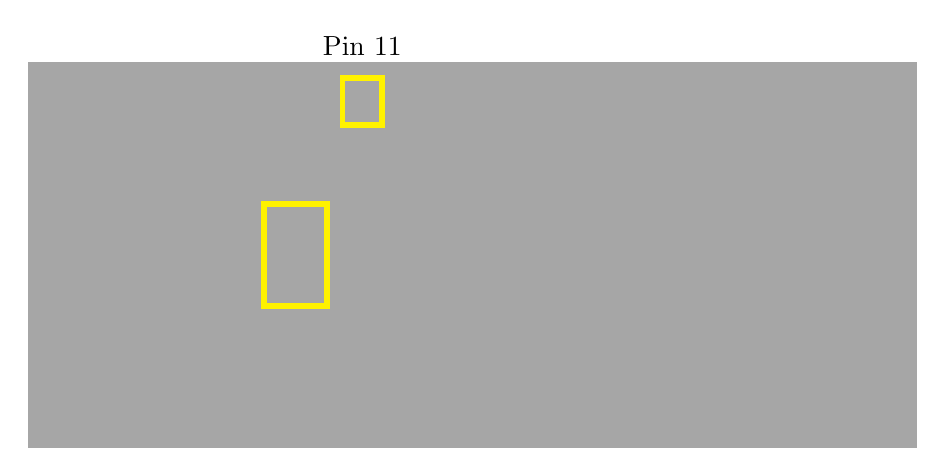
\begin{tikzpicture}
        %\node at (0,0) (Board) {\includegraphics{Arduino/Nano33BLE/Nano33BLESense}};
        
        \ArduinoNanoTikz;
        
        \fill[gray, opacity=0.7] (-11.2,-0.2) rectangle (0.1,4.7);
        
        \coordinate (A) at (-8.2,1.6);
        \coordinate (B) at (-7.4,2.9); 
        
        
        \coordinate (C) at (-7.2,3.9);
        \coordinate (D) at (-6.7,4.5);  
        
        \def\cliparea{(C) rectangle (D); (A) rectangle (B); }  
        
        \begin{scope}
            \clip (A) rectangle (B);
            
            \ArduinoNanoTikz
            
            %\node at (0,0) (Board) {\includegraphics{Arduino/Nano33BLE/Nano33BLESense}};
            
        \end{scope}
        
        %        \fill[ArduinoColor] (C) rectangle (D);
        %         \fill[gray!30] ({-8.16-0.195},4.145) rectangle ++(0.39, 0.39); 
        %        \draw[fill=gray!30,gray!30] (-8.145,4.143) circle(0.195); 
        %        \draw[fill=gray!60,gray!60] (-8.145,4.143) circle(0.165); 
        %        \fill[white,white](-8.145,{4.143+0.39}) circle (0.1275);
        
        \draw[yellow,line width=2pt] (A)  rectangle (B);
        \draw[yellow,line width=2pt] (C)  rectangle (D);
        
        \node (P25) at (-6.95, 4.9) {Pin 11};
    \end{tikzpicture}    
    
    
    
    \captionof{figure}{Arduino Nano 33 BLE Sense's built-in Push Button  with Pin 11}  
\end{center}

}






\section{Specification}

The built-in button is a small white button  and connected to pin 11.\index{Pin!Pin 11}

\begin{description}
    \item [Built-in Button:] \PYTHON{BUTTON\_B =  11u}
\end{description}

If the pin is declared as input in the function \PYTHON{setup}, then it can be used.

%\Mynote{cite data sheet, power consumption?}

The pin 11 must be defined as an input in the function \PYTHON{setup} by setting \PYTHON{pinMode (11, INPUT\_PULLUP)}, otherwise the button cannot be read.

\medskip 


The pin 11 can also be used otherwise. Then the button is not in use. \cite{Arduino:2023a,Arduino:2023,ArduinoNano33Manual:2022}

%\Mynote{What happen if there is another button at the pin? Both in use?}

\Mynote
{
\begin{itemize}
  \item cite data sheet
  \item Circuit Diagram
\end{itemize}
}

\section{Simple Code}


As soon as the button is connected, it can be used. It is not necessary to install a special library. Programming takes place in two steps:

\begin{enumerate}
    \item In the first step, the pin is configured in the function \PYTHON{setup}:
    
    {
        \captionof{code}{Defining the built-in button's pin as an input.}
        \begin{Arduino}
            pinMode(BUTTON_B, INPUT_PULLUP)   
        \end{Arduino}
    }
    \item In the second step, the button can be used in the function \PYTHON{loop}. To read in the value, use the function \PYTHON{digitalRead}:
    
    {
        \captionof{code}{Read the built-in button's state}
        \begin{Arduino}
            buttonState = digitalRead(BUTTON_B);
        \end{Arduino}
    }
    
\end{enumerate}




\section{Tests}


The simplest test is the flashing of an LED for 2 seconds, if the button is pressed, see sketch \ref{Nano:BuiltinButtonTest}.

{
    \captionof{code}{Simple sketch to test the push button and the built-in LED}\label{Nano:BuiltinButtonTest}
    \ArduinoExternal{}{../../Code/Nano33BLESense/PushButton/TestPushButton/TestPushButton.ino}
}

\section{Interrupt Function on the Arduino Nano 33 BLE Sense}


An interrupt is a function that allows the microcontroller on the Arduino Nano 33 BLE Sense to immediately respond to an external event, such as pressing a button, without the need for the program to continuously check for that event. Normally, in a program, the microcontroller would repeatedly check if a button is pressed by running through a loop, which consumes processing power and can slow down other tasks. This is not efficient, especially when the program needs to perform other actions at the same time.

With an interrupt, the program can continue running other tasks, and only when the specified event (like a button press) occurs, the program is temporarily paused to execute a special function known as the \menu{Interrupt Service Routine (ISR)}. The ISR is a small, efficient function designed to handle the event, such as changing a variable or triggering another action. After the ISR is executed, the program returns to where it left off, continuing its normal operation.

Using interrupts in this way helps make the program more efficient and responsive, as it doesn't waste time constantly checking for events and can focus on other tasks until something important happens. This is especially useful for real-time applications where quick responses to external events are necessary, such as in embedded systems, robotics, or sensor monitoring.



\section{Simple Application}



This code sketch \ref{Nano:TestButtonInterrupt} shows how to use an interrupt to control the built-in LED on the Arduino Nano 33 BLE Sense when the built-in push button is pressed.

The program sets up the built-in LED and push button. When the button is pressed, an interrupt runs a special function called an Interrupt Service Routine. The ISR is very short and only sets a flag variable \PYTHON{pushPressed} to \PYTHON{true}, indicating that the button has been pressed.

The main program \PYTHON{loop} checks this flag. If it is set to \PYTHON{true}, the program turns on the LED for 2 seconds, then turns it off and resets the flag to \PYTHON{false}. This ensures the system is ready to detect the next button press. Using the \PYTHON{true and false} values makes it easy to manage the button's state.

This method avoids constantly checking the button’s state, making the program more efficient. Additionally, the Arduino Nano 33 BLE Sense allows all its pins to be used for interrupts. This makes it easy to attach interrupt functions to any pin, allowing quick and efficient responses to inputs like buttons or sensors. \cite{ArduinoInterrupt:2019}


\Mynote{andere Überschrift für simple Application}

\bigskip







{
    \captionof{code}[Simple sketch connects the push button with an interrupt.]{Simple sketch connects the push button with an interrupt. Here, pushing the built-in button is handled by an interrupt. Then the built-in LED switch on for 2 sec.}\label{Nano:TestButtonInterrupt}
    \ArduinoExternal{}{../../Code/Nano33BLESense/PushButton/TestPushButtonInterrupt/TestPushButtonInterrupt.ino}
}

\bigskip

This is just a simple example. The variable \PYTHON{BUTTON\_B} is already defined, so the assignment is not necessary. The command \PYTHON{delay} should be avoided in an Arduino sketch. Instead, variables of the type \PYTHON{elapsedMillis} should be used.



\section{Further Readings}

\begin{itemize}
  \item Boxall, John: \textsl{Arduino Workshop - A Hands-On Introduction with 65 Projects}. No Starch Press, 2021. \cite{Boxall:2021}
  \item Vo{\"s}, Andreas: \textsl{Volumio mit Drehgebern erweitern}. Make Magazin, 2024. \cite{Voss:2024}
  \item K\"uhnel, Claus: \textsl{Arduino - Das umfassende Handbuch}. Rheinwerk Verlag GmbH, 2024. \cite{Kuehnel:2024}
\end{itemize}



  %%%%%%%%%%%%
%
% $Autor: Wings $
% $Datum: 2019-03-05 08:03:15Z $
% $Pfad: TemplateSensor $
% $Version: 4250 $
% !TeX spellcheck = en_GB/de_DE
% !TeX encoding = utf8
% !TeX root = filename 
% !TeX TXS-program:bibliography = txs:///biber
%
%%%%%%%%%%%%

% Structure
\chapter{Pressure and Temperature Sensor LPS22HB}

The sensor LPS22HB is a piezoresistive absolute pressure sensor that is integrated into the Arduino Nano 33 BLE Sense board. It's a digital sensor that measures atmospheric pressure and temperature. The sensor uses a piezoresistive technology to detect changes in pressure. The LPS22HB has an accuracy of $\pm1.5$ hPa and a resolution of 0.01 hPa. It can measure pressures from 260 to 1260 hPa. The sensor also measures temperature with an accuracy of $\pm0.12^\circ$C and a resolution of $0.01^\circ$C. The temperature range is from $-40^\circ$C to $85^\circ$C. 

The LPS22HB communicates with the Arduino board using the protocol I\textsuperscript{2}C. It has a low power consumption of 1.5 $\mu A$ in sleep mode and 1.5 mA in active mode. The sensor is also resistant to shock and vibration. It's a sensor for projects that require accurate pressure and temperature measurements, such as weather stations, altimeters. \cite{Arduino:2023a,Arduino:2023}

Arduino Nano 33 BLE Sense Lite hat  keine HTS221-Temperatur- und Feuchtigkeitssensoren, sondern nur den LPS22HB-Drucksensor, der allerdings auch die Temperatur messen kann

Arduino Nano 33 BLE Sense Rev2 hat  einen HTS221-Temperatur- und Feuchtigkeitssensor und den LPS22HB-Drucksensor, der allerdings auch die Temperatur messen kann.


Unterschiede:

Inertiale Messeinheit (IMU):
Rev 1: Verfügt über eine einzelne 9-Achsen-IMU.
Rev 2: Hat eine Kombination aus zwei IMUs: eine 6-Achsen-IMU (BMI270) und eine 3-Achsen-IMU (BMM150), was die Möglichkeiten zur Bewegungserkennung erweitert1.

Design und Zugänglichkeit:
Rev 2: Integriert neue Pads und Testpunkte für USB, SWDIO und SWCLK, was den Zugang zu diesen wichtigen Punkten auf der Platine erleichtert1.
Rev 1: Hat diese zusätzlichen Pads und Testpunkte nicht.
Stromversorgung:

Rev 2: Verwendet den MP2322 als Stromversorgungskomponente, was die Leistung verbessert1.

Rev 1: Nutzt eine andere Stromversorgungskomponente.
Der Arduino Nano 33 BLE Sense Rev 1 verwendet den MPS MP2144 als Stromversorgungskomponente

\begin{center}    
    
\begin{tikzpicture}
        %\node at (0,0) (Board) {\includegraphics{Arduino/Nano33BLE/Nano33BLESense}};
        
        \ArduinoNanoTikz;
        
        \fill[gray, opacity=0.7] (-11.2,-0.2) rectangle (0.1,4.7);
        
        \coordinate (A) at (-6.55,2.4);
        \coordinate (B) at (-5.9,3.05);    
        
        
        
        \begin{scope}
            \clip (A) rectangle (B);
            
            \ArduinoNanoTikz
            
            %\node at (0,0) (Board) {\includegraphics{Arduino/Nano33BLE/Nano33BLESense}};
            
        \end{scope}
        
        
        \draw[yellow,line width=2pt] (A)  rectangle (B);        
    \end{tikzpicture}    
    
    \captionof{figure}{Arduino Nano 33 BLE Sense's pressure and temperature sensor LPS22HB}  
\end{center}




\section{General}

A pressure sensor is a device that measures the pressure of its surroundings. It works by converting the mechanical energy of the environment into an electrical signal. The sensor typically consists of a diaphragm or membrane, which is a thin, flexible material that changes its shape in response to changes in pressure. The diaphragm or membrane is usually connected to a microcontroller or other electronic device, which reads the electrical signal and converts it into a pressure reading. The pressure sensor can be calibrated to provide accurate readings over a specific pressure range. The sensor can be used in a variety of applications, including industrial control systems, medical devices, and consumer electronics.

Pressure sensors can be classified into two main types: absolute and differential. Absolute pressure sensors measure the absolute pressure of the environment, while differential pressure sensors measure the difference in pressure between two points. Pressure sensors can be used to measure a wide range of pressures, from very low pressures to very high pressures. The accuracy of a pressure sensor depends on its calibration and the quality of its components. Pressure sensors can be affected by various factors, including temperature, humidity, and air flow. Pressure sensors can be used to monitor and control pressure in a variety of applications, including heating and cooling systems, refrigeration systems, and food processing systems. Pressure sensors can be used to detect pressure anomalies and alert users to potential problems. \cite{Gan:2024}

\bigskip

% temperatur
A temperature sensor is a device that measures the temperature of its surroundings. It works by converting the thermal energy of the environment into an electrical signal. The sensor typically consists of a thermistor or thermocouple, which is a device that changes its electrical resistance or voltage in response to changes in temperature. The thermistor or thermocouple is usually connected to a microcontroller or other electronic device, which reads the electrical signal and converts it into a temperature reading. The temperature sensor can be calibrated to provide accurate readings over a specific temperature range. The sensor can be used in a variety of applications, including industrial control systems, medical devices, and consumer electronics.

Temperature sensors can be classified into two main types: contact and non-contact. Contact temperature sensors, such as thermocouples, come into direct contact with the object being measured. Non-contact temperature sensors, such as infrared sensors, do not come into contact with the object being measured.

Temperature sensors can be used to measure a wide range of temperatures, from very low temperatures to very high temperatures. The accuracy of a temperature sensor depends on its calibration and the quality of its components. Temperature sensors can be affected by various factors, including humidity, air flow, and radiation. Temperature sensors can be used to monitor and control temperature in a variety of applications, including heating and cooling systems, refrigeration systems, and food processing systems. Temperature sensors can be used to detect temperature anomalies and alert users to potential problems.



\Mynote{cite books, applications, board}

\section{Specific Sensor}

The pressure sensor of the LPS22HB is a piezoresistive sensor that changes its electrical resistance in response to changes in pressure. The pressure sensor of the LPS22HB is connected to the Arduino Nano 33 BLE Sense, which reads the electrical signal and converts it into a pressure reading. The pressure sensor of the LPS22HB is calibrated to provide accurate readings over a pressure range of 260 to 1260 mbar. The pressure sensor of the LPS22HB is a non-contact sensor, meaning that it does not come into direct contact with the object being measured. The pressure sensor of the LPS22HB is affected by various factors, including temperature and humidity. The pressure sensor of the LPS22HB can be used to monitor and control pressure in a variety of applications, including industrial control systems and consumer electronics. The pressure sensor of the LPS22HB can be used to detect pressure anomalies and alert users to potential problems. The pressure sensor of the LPS22HB has an accuracy of $\pm0.12$ mbar. 

The pressure sensor of the LPS22HB is a low-power sensor, making it suitable for use in battery-powered devices. 

\bigskip
% Temperatur

The LPS22HB is a digital pressure sensor that also includes a temperature sensor. The temperature sensor of the LPS22HB is a thermistor that changes its electrical resistance in response to changes in temperature. The thermistor is connected to the  microcontroller Arduino Nano 33 BLE Sense, which reads the electrical signal and converts it into a temperature reading. The temperature sensor of the LPS22HB is calibrated to provide accurate readings over a temperature range of $-40^\circ$C to $85^\circ$C. The temperature sensor of the LPS22HB is a non-contact sensor, meaning that it does not come into direct contact with the object being measured. 

The temperature sensor of the LPS22HB is affected by various factors, including humidity and air flow. The temperature sensor of the LPS22HB can be used to monitor and control temperature in a variety of applications, including industrial control systems and consumer electronics. The temperature sensor of the LPS22HB can be used to detect temperature anomalies and alert users to potential problems. The temperature sensor of the LPS22HB is a high-accuracy sensor, with an accuracy of $\pm0.12^\circ$C and a resolution of $0.01^\circ$C. 

The temperature sensor of the LPS22HB is a low-power sensor, making it suitable for use in battery-powered devices. 

\Mynote{cite board}

\section{Specification}

The LPS22HB is a digital pressure sensor that measures pressure in the range of 260 to 1260 mbar. It has a high accuracy of $\pm0.12$ mbar and a resolution of 0.01 mbar. The sensor is calibrated to provide accurate readings over a temperature range of $-40^\circ$C to $85^\circ$C. It has a non-contact measurement principle, which means that it does not come into direct contact with the object being measured. The LPS22HB is a compact sensor, measuring $3.5 \times 3.5 \times 1.1$ mm in size. 

It has a low power consumption of $1.5 \mu A$ in active mode and $0.1 \mu A$ in sleep mode.

The sensor has a sampling rate of up to 100 Hz and a data transfer rate of up to 400 kbps. Note that the sampling rate of the sensor LPS22HB can be adjusted using the function \PYTHON{setSamplingRate()} in the Arduino library. The default sampling rate is 100 Hz, but it can be set to 50 Hz, 25 Hz, or 10 Hz using the following code:

\medskip

\PYTHON{lps22hb.setSamplingRate(50); // 50 Hz}

\PYTHON{lps22hb.setSamplingRate(25); // 25 Hz}

\PYTHON{lps22hb.setSamplingRate(10); // 10 Hz}

\medskip


It's worth noting that the sampling rate of the sensor LPS22HB can affect the accuracy and reliability of the measurements. A higher sampling rate can provide more accurate measurements, but it can also increase the power consumption of the sensor.


 The sensor is also resistant to shock, vibration, and temperature changes. It has a high sensitivity and a low noise level, making it suitable for use in applications where high accuracy is required. 



\begin{itemize}
  \item cite data sheet
  \item Circuit Diagram
\end{itemize}

\section{Library}

To program the sensor LPS22HB on the Arduino Nano 33 BLE Sense, you will need to use the library LPS22HB. \cite{ArduinoLPS22HB:2024}

\subsection{Description}

The library LPS22HB is a library for the Arduino platform that provides a simple interface for interacting with the sensor LPS22HB. It allows you to read temperature and pressure values from the sensor, as well as set the sensor's mode and power mode. \cite{ArduinoLPS22HB:2024}


\subsection{Installation}

To use the library LPS22HB, you will need to install it on your Arduino IDE. You can do this by following these steps:

\begin{itemize}
    \item Open the Arduino IDE and navigate to the menu \menu{Sketch}.
    \item Select \menu{Sketch -> Include Library -> Manage Libraries}.
    \item Search for ``LPS22HB'' in the library search bar.
    \item Click on the library ``LPS22HB''  and then click on the buttion ``Install''.
    \item Wait for the library to install and then restart the Arduino IDE.
\end{itemize}

\medskip

Once you have installed the library LPS22HB, you can use it to program the sensor LPS22HB on the Arduino Nano 33 BLE Sense. Here is an example~\ref{LPS22HBSimpleExample} of how you can use the library to read temperature and pressure values from the sensor:

\medskip

{
    \captionof{code}{Example code for the sensor LPS22HB on the Arduino Nano 33 BLE Sense}\label{LPS22HBSimpleExample.ino}
    \ArduinoExternal{}{../../Code/Nano33BLESense/SensorLPS22HB/LPS22HBSimpleExample.ino}
}

\medskip

This sketch \ref{LPS22HBSimpleExample.ino} uses the library LPS22HB to read temperature and pressure values from the sensor LPS22HB and print them to the serial console.

Note that you will need to have the Arduino Nano 33 BLE Sense board connected to your computer and the Arduino IDE installed on your computer in order to use the LPS22HB library.


\subsection{Functions}
Here are the functions of the Arduino library LPS22HB:

\begin{itemize}
  \item Initialization Functions
    \begin{itemize}
      \item \PYTHON{begin()}: Initializes the sensor LPS22HB and sets it up for use.
      \item \PYTHON{reset()}: Resets the sensor LPS22HB to its default state.
    \end{itemize}
  \item Reading Functions
    \begin{itemize}
      \item \PYTHON{readTemperature()}: Reads the temperature value from the sensor LPS22HB.
      \item \PYTHON{readPressure()}: Reads the pressure value from the sensor LPS22HB.
      \item \PYTHON{readAltitude()}: Reads the altitude value from the sensor LPS22HB.
      \item \PYTHON{readTemperatureAndPressure()}: Reads both the temperature and pressure values from the sensor LPS22HB.
    \end{itemize}
  \item Setting Functions
    \begin{itemize}
      \item \PYTHON{setMode()}: Sets the mode of the sensor LPS22HB.
      \item \PYTHON{setPowerMode()}: Sets the power mode of the sensor LPS22HB.
      \item \PYTHON{setSamplingRate()}: Sets the sampling rate of the sensor LPS22HB.
      \item \PYTHON{setFilter()}: Sets the filter of the sensor LPS22HB.
    \end{itemize}
  \item Getting Functions
    \begin{itemize}
      \item \PYTHON{getMode()}: Gets the current mode of the sensor LPS22HB.
      \item \PYTHON{getPowerMode()}: Gets the current power mode of the sensor LPS22HB.
      \item \PYTHON{getSamplingRate()}: Gets the current sampling rate of the sensor LPS22HB.
      \item \PYTHON{getFilter()}: Gets the current filter of the sensor LPS22HB.
    \end{itemize}
  \item Sleep Functions
    \begin{itemize}
      \item \PYTHON{sleep()}: Puts the sensor LPS22HB into sleep mode.
      \item \PYTHON{wakeUp()}: Wakes up the sensor LPS22HB from sleep mode.
    \end{itemize}
  \item Other Functions
    \begin{itemize}
      \item \PYTHON{checkStatus()}: Checks the status of the sensor LPS22HB.
      \item \PYTHON{getError()}: Gets the error code of the sensor LPS22HB.
      \item \PYTHON{resetError()}: Resets the error code of the sensor LPS22HB.
    \end{itemize}
\end{itemize}

\medskip

Note that this list may not be exhaustive, and the library may have additional functions not listed here.

\subsection{Example - Manual}

\subsection{Example}

\subsection{Example - Code}

\subsection{Example - Files}



\section{Calibration}

To calibrate the sensor LPS22HB on the Arduino Nano 33 BLE Sense, you will need to follow these steps. First, upload the calibration code to the Arduino Nano 33 BLE Sense. The calibration code will prompt you to enter the calibration parameters, such as the temperature and pressure values. Enter the calibration parameters, and the code will store them in the sensor's memory. The calibration process will take a few minutes to complete. During the calibration process, the sensor will take multiple readings of the temperature and pressure values. The sensor will then calculate the average of the readings and store it as the calibration value. Once the calibration process is complete, the sensor will be ready to use. To verify the calibration, you can use the calibration code to read the temperature and pressure values from the sensor. Compare the readings with the expected values to ensure that the sensor is calibrated correctly. If the readings are not accurate, you may need to repeat the calibration process. The calibration process can be repeated as many times as necessary to achieve accurate readings. The calibration values can be stored in the sensor's memory and retrieved later. By following these steps, you can calibrate the sensor LPS22HB on the Arduino Nano 33 BLE Sense and ensure accurate readings.

\Mynote{cite method, more mathematics!}




The code \ref{LPS22HBCalibration.ino} reads the temperature and pressure values from the sensor LPS22HB, stores them in the sensor's memory, and prints them to the serial console. The storeCalibration function is used to store the calibration values in the sensor's memory.

\medskip

{
    \captionof{code}{Simple sketch calibrating the sensor LPS22HB}\label{LPS22HBCalibration.ino}
    \ArduinoExternal{}{../../Code/Nano33BLESense/SensorLPS22HB/LPS22HBCalibration.ino}
}

\medskip


Note that this is just an example code and you may need to modify it to suit your specific needs. Additionally, you will need to make sure that the sensor LPS22HB is properly connected to the Arduino Nano 33 BLE Sense and that the I2C interface is enabled.

\section{Simple Code}

\section{Sleep Mode}



{
    \captionof{code}{Sketch for the Arduino Nano 33 BLE Sense to switch the sensor LPS22HB into sleep mode}\label{LPS22HBSleep.ino}
    \ArduinoExternal{}{../../Code/Nano33BLESense/SensorLPS22HB/LPS22HBSleep.ino}
}

\medskip


This sketch \ref{LPS22HBSleep.ino} uses the function \PYTHON{sleep()} to switch the sensor into sleep mode, and the function \PYTHON{wakeUp()} to switch the sensor out of sleep mode. The function \PYTHON{sleep()} puts the sensor into a low-power state, and the function \PYTHON{wakeUp()} restores the sensor to its normal operating state.

Note that the function \PYTHON{sleep()} must be called before the sensor can be put into sleep mode, and the function \PYTHON{wakeUp()} must be called before the sensor can be restored to its normal operating state.

Also, note that the function \PYTHON{sleep()}  can only be called when the sensor is in a valid state, and the function \PYTHON{wakeUp()} can only be called when the sensor is in a valid state.

You can also use the function \PYTHON{setMode()} to set the sensor to sleep mode, and the function \PYTHON{getMode()} to get the current mode of the sensor.

\medskip

\PYTHON{lps22hb.setMode(LPS22HB\_MODE\_SLEEP);}

\PYTHON{lps22hb.getMode();}

\medskip

This will set the sensor to sleep mode and get the current mode of the sensor.

You can also use the function \PYTHON{setPowerMode()}  to set the power mode of the sensor, and the function \PYTHON{getPowerMode()} to get the current power mode of the sensor.

\medskip

\PYTHON{lps22hb.setPowerMode(LPS22HB\_POWER\_MODE\_SLEEP);}

\PYTHON{lps22hb.getPowerMode();}


This will set the power mode of the sensor to sleep mode and get the current power mode of the sensor.

\section{Simple Application}



\section{Tests}

\subsection{Simple Function Test}

\subsection{Test all Functions}

\section{Simple Application}


\section{Further Readings}



 % %%%%%%%%%%%%%%%
%
% $Autor: Wings $
% $Datum: 2020-01-29 07:55:27Z $
% $Pfad: General/SensorAPDS9960.tex
% $Version: 1785 $
%
%
%%%%%%%%%%%%%%%

\chapter{Sensormodul APDS-9960 for Gesture, Proximity, and Color Detection}

The APDS-9960 sensor, integrated on the Arduino Nano 33 BLE Sense, is a multifunctional optical sensor used for gesture recognition, ambient light detection, color sensing, and proximity measurement. The sensor uses an I²C interface for communication and comes equipped with an additional infrared LED.
\cite{Avago:2015}


\begin{center}    
	\begin{tikzpicture}
		\node at (0,0) (Board) {\includegraphics{Arduino/Nano33BLE/Nano33BLESense}};
		
		\fill[gray, opacity=0.7] (-6,-2.4) rectangle (6,2.4);
		
		\coordinate (A) at (-1,0.4);
		\coordinate (B) at (0.2,-0.2);    
		\begin{scope}
			\clip (A) rectangle (B);
			\node at (0,0) (Board) {\includegraphics{Arduino/Nano33BLE/Nano33BLESense}};
		\end{scope}
		\draw[yellow,line width=2pt] (A) rectangle (B);
	\end{tikzpicture}    
	
	\captionof{figure}{Arduino Nano 33 BLE Sense's APDS-9960}
	\label{fig:5.1}
\end{center}

\bigskip


\Mynote{Figure 6.1 must be converted into a TikZ image to maintain consistency}

The sensor is located centrally on the Arduino Nano 33 BLE Sense, as indicated in the Figure \ref{fig:5.1}.










\section{Functionality of the APDS-9960}


The APDS-9960 is a versatile optical sensor that offers multiple functionalities, including color detection, proximity sensing, ambient light measurement, and gesture recognition. Each of these features plays a crucial role in various applications, ranging from smart lighting adjustments to touchless control systems.

In the following sections, each function of the APDS-9960 will be explored in detail, explaining its working principle, the type of data it provides, and its potential use cases.





\section{Key Technical Specifications}
\label{chap:Specification}

\subsection*{Power Supply}
\begin{itemize}
	\item Supply Voltage: 2.4 V to 3.6 V
	\item Maximum Voltage: 3.8 V
\end{itemize}

\subsection*{Power Consumption}
\begin{itemize}
	\item Active ALS Mode (Ambient Light Sensor): 200-250 µA
	\item Proximity and Gesture Modes: 790 µA (without LED)
	\item Sleep Mode: 1-10 µA
\end{itemize}

\subsection*{Temperature}
\begin{itemize}
	\item Operating Temperature Range: -30°C to +85°C
	\item Storage Temperature Range: -40°C to +85°C
\end{itemize}

\subsection*{Optical Properties}
\begin{itemize}
	\item LED Wavelength (max.): 950 nm
	\item LED Drive Current:
	\begin{itemize}
		\item 100 mA (Standard), 50 mA, 25 mA, 12.5 mA
		\item LED Boost Option: 100\%, 150\%, 200\%, 300\% (adjustable current boost)
	\end{itemize}
	\item Max Detection Distance for Color, Proximity and Gesture Sensor 0mm to 100mm
\end{itemize}

\subsection*{Proximity Sensor}
\begin{itemize}
	\item Pulse Width for Proximity Measurement: 4 µs to 32 µs
\end{itemize}

\subsection*{Gesture Sensor}
\begin{itemize}
	\item LED Pulse Count: 1 to 64 pulses
\end{itemize}

\subsection*{Connections}
\begin{itemize}
	\item I²C Communication:
	\begin{itemize}
		\item Data Rates: Up to 400 kHz
		\item Pins:
		\begin{itemize}
			\item SDA (I²C Data)
			\item SCL (I2C Clock)
			\item INT (Interrupt, Open Drain, Active Low)
			\item LDR (LED Driver Input)
		\end{itemize}
	\end{itemize}
\end{itemize}

\subsection*{Dimensions}
\begin{itemize}
	\item Length: 3.94mm
	\item Width: 2.36mm
	\item Height: 1.35mm
\end{itemize}

\cite{Avago:2015}


\section{Library \PYTHON{Arduino\_APDS9960}}

In the case of the APDS-9960 sensor, Arduino provides a library \FILE{Arduino\_APDS9960} for calling functions related to color detection, distance measurement, or gesture recognition.

The library for the sensor is \FILE{Arduino\_APDS9960}. This allows measuring gestures, colors, light intensity, and distances with the sensor. Communication between the Arduino Nano 33 BLE Sense's chip and the APDS-9960 module occurs via an internal I²C interface \cite{Avago:2015}.

The library is included by using the command \PYTHON{\#include <Arduino\_APDS9960.h>}.






\subsection{Installation of APDS-9960 Library}

The library is installed as follows:



\begin{enumerate}
	\item Open the Arduino IDE and navigate to \menu[,]{Tools,Manage Libraries...}.
	\item In the Library Manager, use the search bar to look for "Arduino\_APDS9960".
	\item Several libraries will be displayed. Select the library titled "Arduino\_APDS9960" by Arduino and click \textit{Install}.
	\item Once installed, the IDE will show a message in the console confirming the installation. The "Install" button will also change to "Remove", as seen in Figure \ref{fig:APDS9960}, indicating the library is ready for use.
\end{enumerate}


\begin{center}
	\includegraphics[width=8cm]{Arduino/APDS9960/APDS9960Installed.png}
	\captionof{figure}{APDS-9960 Library Instalation}\label{fig:APDS9960}		
\end{center} 










\subsection{Functions}

After the theoretical overview of the APDS-9960 sensor's functions, the following section will explain the practical implementations. It will demonstrate how the various functions of the sensor, such as color detection, gesture recognition, and proximity sensing, can be applied in practice to activate and evaluate the sensor's capabilities.

\medskip

Here are the codes to utilize the various functions of the APDS-9960 sensor, such as color detection, gesture recognition, and proximity sensing, see \cite{ArduinoAPDS9960:2024}:

\begin{itemize}
	\item \PYTHON{begin()}: The \PYTHON{begin()} method activates and initializes the APDS9960 sensor. It is typically called during the \PYTHON{setup\{\}} phase.
	
	\medskip
	
	\begin{itemize}
		\item Return value \PYTHON{TRUE}: Initialization was successful.
		\item Return value \PYTHON{FALSE}: Initialization failed.
	\end{itemize}
	
	\item \PYTHON{end()}: The \PYTHON{end()} method deactivates the APDS9960 sensor.
	
	
	\item \PYTHON{colorAvailable()}: This method checks if color data is available to be retrieved.
	
	\medskip
	
	\begin{itemize}
		\item Return value \PYTHON{TRUE}: Color data is available.
		\item Return value \PYTHON{FALSE}: No color data is available.
	\end{itemize}
	
	\item \PYTHON{readColor(...)}: This method retrieves the color values from the sensor.
	
	It can either read just the color values or the color values along with the ambient light intensity.
	
	\medskip
	
	To read only the color values:
	
	\PYTHON{int r, g, b;}
	
	\PYTHON{APDS.readColor(r, g, b);}
	
	\medskip
	
	The variables \PYTHON{r}, \PYTHON{g}, and \PYTHON{b} will contain the updated color values. The value range is $0, 1, 2, \ldots, 255$.
	
	\medskip
	
	To read both the color values and ambient light intensity:
	
	\PYTHON{int r, g, b, a;} 
	
	\PYTHON{APDS.readColor(r, g, b, a);}
	
	\medskip
	
	The variables \PYTHON{r}, \PYTHON{g}, and \PYTHON{b} will contain the updated color values, while \PYTHON{a} will contain the ambient light intensity. The value range is $0, 1, 2, \ldots, 255$.
	
	\item \PYTHON{proximityAvailable()}: This method checks if proximity data is available.
	
	\medskip
	
	\begin{itemize}
		\item Return value \PYTHON{TRUE}: Proximity data is available.
		\item Return value \PYTHON{FALSE}: No proximity data is available.
	\end{itemize}
	
	\item \PYTHON{readProximity()}: This method reads the proximity value.
	
	\medskip
	
	\begin{itemize}
		\item Return value \PYTHON{int proximity = APDS.readProximity()}: Returns the proximity value.
		\item Return value \PYTHON{-1}: Proximity could not be determined.
	\end{itemize}
	
	\item \PYTHON{gestureAvailable()}: This method checks if a gesture has been detected.
	
	\medskip
	
	\begin{itemize}
		\item Return value \PYTHON{TRUE}: A gesture has been detected.
		\item Return value \PYTHON{FALSE}: No gesture detected.
	\end{itemize}
	
	\item \PYTHON{setGestureSensitivity()}: Gesture detection is influenced by lighting conditions, speed, and distance of movement. This function allows you to adjust the sensitivity of gesture recognition. A higher value detects more gestures, but increases the chance of false positives. A lower value reduces the likelihood of detecting gestures.
	
	The valid range is \PYTHON{1} to \PYTHON{100}.
	
	The default value is \PYTHON{80}.
	
	\item \PYTHON{readGesture()}: If a gesture has been detected, it can be retrieved using the \PYTHON{readGesture()} method. The possible return values are:
	
	\begin{itemize}
		\item \PYTHON{GESTURE\_UP}: An upward movement has been detected.
		\item \PYTHON{GESTURE\_DOWN}: A downward movement has been detected.
		\item \PYTHON{GESTURE\_LEFT}: A leftward movement has been detected.
		\item \PYTHON{GESTURE\_RIGHT}: A rightward movement has been detected.
		\item \PYTHON{GESTURE\_NONE}: No gesture has been detected.
	\end{itemize}
	
	\item \PYTHON{setInterruptPin()}: This method sets the pin used to trigger a measurement. The pin is usually detected automatically, but can be set manually using this function.
	
	If \PYTHON{-1} is passed, no pin is connected.
	
	If \PYTHON{0} or a higher value is passed, that pin will be used.
	
	The default value depends on the board.
	
	\item \PYTHON{setLEDBoost(...)}: The sensor includes an infrared LED that can be temporarily boosted to provide higher brightness. It can be set to provide up to 300\% of its normal power. This can be configured using this method.
	
	\medskip
	
	Usage:
	
	\begin{itemize}
		\item \PYTHON{0}: Boost to 100\% (default power).
		\item \PYTHON{1}: Boost to 150\%.
		\item \PYTHON{2}: Boost to 200\%.
		\item \PYTHON{3}: Boost to 300\%.
	\end{itemize}    
	
	\medskip
	
	Return values:
	
	\begin{itemize}
		\item \PYTHON{0}: Failure.
		\item \PYTHON{1}: Success.
	\end{itemize}
\end{itemize}




\section{Simple Function Tests}

The following code examples can be used to test and try out all functions of the APDS-9960.

\subsection{Example Color Detection}

The library  \PYTHON{Arduino\_APDS9960} includes an example code demonstrating how to perform color detection with the sensor APDS-9960 on an Arduino Nano 33 BLE Sense. This example also tests the ambient light sensor, as both functionalities rely on the same underlying technology. The measured color channel intensities (Red, Green, and Blue) are displayed in the Serial Monitor for real-time observation.

The sensor APDS-9960 enables accurate RGB color detection by measuring the intensity of red, green, and blue light reflected from an object. These values can be visualized in the Serial Plotter, allowing users to track changes in color intensity over time through a graphical representation. This feature is particularly useful for applications that require real-time color monitoring or dynamic light adjustments.


\subsection{Example Color Detection - Manual}

\Mynote{to do}


\subsection{Setting Up the Color Sensor Measurement Program}

To begin the process of creating the color sensor measurement program, open the Arduino Cloud Editor and navigate to the "Libraries" tab. Search for the "Arduino-APDS9960" library and download it. Afterward, click on "More info" to access the GitHub repository, where several examples are provided.

Next, connect the Arduino Nano 33 BLE Sense to the computer, ensuring that the Cloud Editor detects both the board and the corresponding port. If the board is not automatically recognized, follow the instructions to install the necessary plugin to enable the editor to detect the board. Confirm that the correct port is selected. Finally, upload the program to the Arduino, and by opening the serial monitor, the measured values will be recorded in the Arduino IDE.

\subsection{Example }Color Detection - Code}

First, serial communication is started with \PYTHON{Serial.begin(9600)} to send data to the computer. The command  \PYTHON{APDS.begin()} initializes the sensor and in the event of a potential error, an error message is output via the serial interface.

\bigskip



\bigskip

The code operates within the function \PYTHON{loop()} of a sketch to continuously read and display color values from the APDS-9960 sensor. Initially, it checks if a color reading is available by using the method \PYTHON{APDS.colorAvailable()}. If no reading is available, the program briefly pauses for 5 milliseconds to avoid excessive CPU usage. Once a reading is ready, the method \PYTHON{APDS.readColor(r, g, b)} retrieves the color data and stores the red, green, and blue values in the respective variables. These values are then printed to the Serial Monitor, labeled clearly as ``r'', ``g'', and ``b''. A one-second delay is added before the program repeats the loop, allowing for clear intervals between consecutive readings.




\subsection{Example Color Detection - File}

The program can be found at 

\medskip

{
	\captionof{code}{Simple sketch using the sensor APDS9960 for colors}\label{TestAPDS9960Color}
	\ArduinoExternal{}{../../Code/Nano33BLESense/APDS9960/TestAPDS9960Color/TestAPDS9960Color.ino}
}


\subsection{Proximity}

A simple code for testing the proximity sensor is also provided by the library. The proximity sensor is designed for measuring distances of up to 100mm.

\subsection{Proximity - Manual}

Open the Arduino Cloud Editor and navigate to the Libraries tab. In the search bar, search for the library \PYTHON{Arduino\_APDS9960}. Once located, open the Examples section within the library and select the sketch ``ProximitySensor''.
\smallskip
Connect the Arduino Nano 33 BLE Sense to the computer. Check that the Cloud Editor recognizes the board by verifying if both the board and port are listed in the dropdown menu.

\subsection{Example Proximity - Code}

First, serial communication is started with \PYTHON{Serial.begin(9600)} to send data to the computer. The method \PYTHON{APDS.begin()}  initializes the sensor and in the event of a potential error, an error message is output via the serial interface.


\bigskip


The code operates within the function \PYTHON{loop()}  of a sketch to continuously read and display proximity values from the sensor APDS-9960. It begins by checking if a proximity reading is available using the method \PYTHON{APDS.proximityAvailable()}. If a reading is ready, the method \PYTHON{APDS.readProximity()} retrieves the proximity value, where \PYTHON{0} indicates a close object, \PYTHON{255} indicates a distant object, and \PYTHON{-1} signals an error in reading. This proximity value is then printed to the Serial Monitor. A delay of 100 milliseconds is added before the program repeats the loop, ensuring a brief interval between consecutive readings.


\subsection{Example Proximity - File}

The sketch can be found at 

\bigskip

{
	\captionof{code}{Simple sketch using the sensor APDS9960 for measuring the proximity}\label{TestAPDS9960Proximity}
	\ArduinoExternal{}{../../Code/Nano33BLESense/APDS9960/TestAPDS9960Proximity/TestAPDS9960Proximity.ino}
}

\subsection{Gesture Detection}
\subsection{Example Gesture Detection}

The library \FILE{Arduino\_APDS9960} also provides an example sketch demonstrating gesture detection with the sensor APDS-9960 on an Arduino Nano 33 BLE Sense. Some LED feedback signals have been programmed to provide quick visual feedback.

\subsection{Example Gesture Detection - Manual}

\Mynote{to do}


\subsection{Example Gesture Detection - Code}

In this example sketch, the library \FILE{Arduino\_APDS9960} is integrated first and then the setup is created. In addition, the LED pins are configured so that they behave as outputs.


\bigskip

After that, serial communication is initialized, and the program verifies whether the sensor is correctly initialized using \PYTHON{APDS.begin()}. If initialization fails, an error message is printed. The gesture sensitivity can be adjusted via \PYTHON{APDS.setGestureSensitivity(value)}, where values range from 1 to 100, affecting detection accuracy and sensitivity. The sketch sets a default sensitivity and signals the start of gesture detection by turning off the RGB LEDs with \PYTHON{digitalWrite(LEDR, HIGH)}, \PYTHON{digitalWrite(LEDG, HIGH)}, and \PYTHON{digitalWrite(LEDB, HIGH)}.

In the function \PYTHON{loop()}, the code continuously checks for available gestures using \PYTHON{APDS.gestureAvailable()}. When a gesture is detected, it is read using \PYTHON{APDS.readGesture()} and interpreted within a \PYTHON{switch} statement. Each gesture corresponds to specific LED behavior:

\begin{itemize}
	\item \PYTHON{GESTURE\_UP}: The red LED is briefly turned on, then off after a 1-second delay.
	\item \PYTHON{GESTURE\_DOWN}: The green LED is briefly turned on, then off after a 1-second delay.
	\item \PYTHON{GESTURE\_LEFT}: The blue LED is briefly turned on, then off after a 1-second delay.
	\item \PYTHON{GESTURE\_RIGHT}: All LEDs are turned on simultaneously, then off after a 1-second delay.
\end{itemize}

The \PYTHON{default} case ensures no action if an undefined gesture is detected.



\subsection{Example Gesture Detection - File}

The sketch can be found at 

\bigskip

{
	\captionof{code}{Simple sketch using the sensor APDS9960 for gesture detection}\label{TestAPDS9960Gesture}
	\ArduinoExternal{}{../../Code/Nano33BLESense/APDS9960/TestAPDS9960Gesture/TestAPDS9960Gesture.ino}
}

\subsection{Troubleshoot}


Errors in color detection can be caused by insufficient lighting in the room. Please ensure that the environment is bright enough for the color detection function.


\section{Calibration Color Detection}

\section{Calibration Color Detection}

Due to variations in environmental light conditions and the sensitivity of the sensor, calibration is required to ensure accurate color detection. This section outlines the calibration process using a standard color chart under constant lighting conditions. To carry out the calibration, the Arduino, a connection cable (USB A to USB Micro), and a laptop or computer with the appropriate Arduino development environment are required.

\medskip

The proximity and gesture feature is pre-configured and factory-calibrated to detect proximity and gesture at a distance of 100mm, eliminating the need for customer calibration.
\cite{BroadcomAPDS9960:2024}

\subsection{Calibration Setup}

A standardized color chart is used, which provides reference values for perfect red, green, and blue under constant lighting conditions. The RGB values from the sensor are read as raw, uncalibrated data, which must be normalized to a standard range (0–255) for accurate color detection.\Mynote{citation, picture}

\subsection{Step 1: Measuring Reference Values}

The first step in the calibration process is to measure the raw sensor values for each primary color (red, green, and blue) using the standardized color chart. By placing the color chart in front of the sensor and reading the raw RGB values, we can establish the maximum possible sensor readings for each color channel.

\[
\text{RawRed} = \max(R_{\text{measured}})
\]
\[
\text{RawGreen} = \max(G_{\text{measured}})
\]
\[
\text{RawBlue} = \max(B_{\text{measured}})
\]

These maximum values are obtained by positioning the chart at a fixed distance of one centimeter and ensuring constant light intensity.

\subsection{Step 2: Normalizing the Sensor Values}
Once the maximum sensor readings for red, green, and blue are obtained, the raw sensor data is normalized to a 0-255 scale. This ensures that the sensor's readings correspond to standard RGB values. The following formula is used for normalization:

\[
R_{\text{calibrated}} = \frac{R_{\text{raw}}}{\text{RawRed}} \times 255
\]
\[
G_{\text{calibrated}} = \frac{G_{\text{raw}}}{\text{RawGreen}} \times 255
\]
\[
B_{\text{calibrated}} = \frac{B_{\text{raw}}}{\text{RawBlue}} \times 255
\]

Where:

\begin{itemize}
	\item $R_{\text{raw}}, G_{\text{raw}}, B_{\text{raw}}$ are the raw sensor values for each channel.
	\item $\text{RawRed}, \text{RawGreen}, \text{RawBlue}$ are the maximum measured values from the standard color chart.
\end{itemize}

\subsection{Step 3: Implementing the Calibration in Code}

The normalization process is implemented directly in the Arduino code to adjust the sensor's readings. To begin calibration, open the Serial Monitor, enter ``OK'' in the command line, and press Enter to confirm. The following steps will then be explained through text output.

\bigskip

After the user initiates the calibration by typing ``OK'' into the Serial Monitor, the sketch starts. The sketch guides the user through the calibration of red, green, and blue colors, with each phase confirmed by entering ``OK''. The pins for the RGB LEDs are defined, and variables store the maximum calibration values for each color. Status variables control the sequence, ensuring each phase is completed before moving to the next. These maximum values are later used for accurate color detection in the Application code.

\bigskip


The following code section begins by initializing serial communication at a baud rate of 9600, enabling interaction through the serial monitor. Next, it sets the RGB LED pins as outputs and turns on all LEDs to create white light, which helps capture accurate color measurements. The code then initializes the sensor APDS-9960, checking for successful setup. If the sensor fails to initialize, an error message is printed, and the program halts. If successful, a message confirms initialization and prompts the user to type ``OK'' in the serial monitor to proceed with the calibration process explanation.

\bigskip

The next code segment in the loop first checks if the user has entered ``OK'' to start the calibration process. After confirmation, it displays an explanation and instructions. After showing the explanation, it waits for the user to confirm by typing ``OK'' again, which then initiates the red color calibration by prompting the user to place the red chart in front of the sensor. The loop pauses at each step until the user confirms.

\Mynote{Screen shot?}

\bigskip

Each color calibration starts after the user types ``OK'' in the Serial Monitor. The sketch measures the highest detected value for each color over 10 seconds and sets it as the calibration maximum. After all colors are calibrated, it displays the final maximum values for red, green, and blue in the Serial Monitor, completing the process. The \PYTHON{maxRed}, \PYTHON{maxGreen}, and \PYTHON{maxBlue} values can later be entered into the application sketch to apply the calibration to the sketch.


\subsection{Calibration File}

The sketch can be found at 

\bigskip

{
	\captionof{code}{APDS-9960: Example Calibration}
	\ArduinoExternal{}{../../Code/Nano33BLESense/APDS9960/APDS9960Calibration/APDS9960Calibration.ino}
}


\subsection{Step 4: Validating the Calibration}

To ensure the calibration is successful, the sensor readings should be tested again using the standard color chart. The calibrated values for red, green, and blue should be close to 255 for the respective pure colors on the chart. If the readings deviate significantly, further adjustment of the maximum reference values may be necessary.

\bigskip

The calibration of the sensor APDS-9960 is essential for accurate RGB detection. By using a standard color chart and constant lighting conditions, the sensor's raw values can be normalized to provide consistent and reliable color readings. This process can be further refined by adjusting for specific environmental factors or sensor placement.


\section{Tests}

\subsection{Simple Function Test}

\subsection{Test all Functions}

\section{Simple Application}

Similarly, by following all the steps for uploading and compiling the sketch we can see the results of sensor APDS-9960  on Serial Monitor, too. For seeing the different output, we can change the input for the sensor too, e.g: for color detection we can switch the colors, for gesture detection we can also switch the gestures, and for proximity also do the same. The resulted output as shown in the figure.  \ref{fig:2} 

\Mynote{rewrite and extend}

\begin{center}
	\includegraphics[width=9.5cm]{Nano33BLESense/APDS-Output}
	\captionof{figure}{Gesture, Proximity, Color Sensor Output Window}
	\label{fig:2}
\end{center}

We can also run the single funcnality of this sensor too, e.g; if we just need to capture the color of product, we can also run the color detection program. It depends upon the application and we can implement our application and modify the code as per our desire results.


{
	\captionof{code}{Simple sketch using the sensor APDS9960}\label{TestAPDS9960}
	\ArduinoExternal{}{../../Code/Nano33BLESense/APDS9960/TestAPDS9960/TestAPDS9960.ino}
}




%%%%%%%%%%%%%%%%%%%%%%%%%%%%%%%%%%


\section{Further Readings}

\begin{itemize}
	%    \item S. Grzesik, R. Kluwak, and B. Plikusinski, "Multispectral Sensor Application Possibility Research for Temperature Measurement," \textit{2023 23rd International Conference on Mechatronics - Mechatronika (ME)}, Brno, Czech Republic, pp. 1-6, 2023. Available at: \url{https://ieeexplore.ieee.org/document/10349583}
	
	\item SparkFun Electronics, ``APDS-9960 RGB and Gesture Sensor Hookup Guide''. A comprehensive guide that explains the functionality of the APDS-9960 and provides step-by-step instructions for implementation. Available at: \url{https://learn.sparkfun.com/tutorials/apds-9960-rgb-and-gesture-sensor-hookup-guide/all}, \cite{Hymel:2024}
	
	\item Maker Guides, ``APDS-9960 Gesture and Color Sensor with Arduino''. This tutorial provides a hands-on introduction to using the APDS-9960 sensor with Arduino, including gesture and color recognition. Available at: \url{https://www.makerguides.com/apds-9960-gesture-and-color-sensor-with-arduino/}, \cite{Maetschke:2024}
\end{itemize}




 % %%%%%%%%%%%%
%
% $Autor: Wings $
% $Datum: 2019-03-05 08:03:15Z $
% $Pfad: TemplateSensor $
% $Version: 4250 $
% !TeX spellcheck = en_GB/de_DE
% !TeX encoding = utf8
% !TeX root = filename 
% !TeX TXS-program:bibliography = txs:///biber
%
%%%%%%%%%%%%

% Structure
\chapter{Sensor APDS 9960 Gesture}

Introduction
\Mynote{cite books, applications, board}



\subsection{Sensormodul APDS 9960 for Gesture}


\subsubsection{Function of the Gesture Detection Sensor}

The gesture recognition of the APDS-9960 is based on four additional angled photodiodes

\begin{itemize}
	
	\item Up – Hand movement upwards.
	\item Down – Hand movement downwards.
	\item Left – Hand movement to the left.
	\item Right – Hand movement to the right.
	
\end{itemize}

which detect reflected infrared light (IR) from the integrated IR-LED. By analyzing the reflection, which measures direction-dependent changes using the photodiodes, the sensor can recognize movements and gestures such as swiping motions in different directions (e.g., up, down, left, right). The sensor converts this information into digital data, such as speed, direction, and distance of the movement. The 32-record FIFO register allows the sensor to temporarily store motion data, ensuring continuous processing.
\smallskip
\cite{Avago:2015}


\section{General}

General description

cite books

\section{Specific Sensor}

cite board

\section{Specification}

\begin{itemize}
  \item cite data sheet
  \item Circuit Diagram
\end{itemize}

\section{Bibliothek}

\subsection{Description}

\subsection{Installation}

\subsection{Functions}

\subsection{Example - Manual}

\subsection{Example}

\subsection{Example - Code}

\subsection{Example - Files}



\section{Calibration}

cite method

\section{Simple Code}


\section{Simple Application}



\section{Tests}

\subsection{Simple Function Test}

\subsection{Test all Functions}

\section{Simple Application}


\section{Further Readings}


 % %%%%%%%%%%%%
%
% $Autor: Wings $
% $Datum: 2019-03-05 08:03:15Z $
% $Pfad: TemplateSensor $
% $Version: 4250 $
% !TeX spellcheck = en_GB/de_DE
% !TeX encoding = utf8
% !TeX root = filename 
% !TeX TXS-program:bibliography = txs:///biber
%
%%%%%%%%%%%%

% Structure
\chapter{Sensor APDS 9960 Color}



The general functionality of a color sensor is based on the reflection of white light from the object to be measured. White light contains wavelengths that cover the entire visible spectrum (p. 189 \cite{Rybach:2013}). Due to the molecular structure of the object or chemical processes, such as photosynthesis, certain wavelengths are absorbed while others are reflected. The reflected light rays that reach the color sensor are spectrally selected by color filters or a diffraction grating  \cite{Hering:2023}. 

\section{General}

\textbf{Color filters}: By using parallel red, green, and blue color filters, the intensities of the RGB components are evaluated by three photodiodes behind the filters \cite{Hering:2023}.

\textbf{Diffraction grating}: As light passes through a diffraction grating, the physical diffraction effect occurs. This effect, due to the varying wavelengths of light, produces an interference pattern that enables the spectral decomposition of the light. The spectrum of the incoming light is spatially dispersed, similar to the refraction in a prism (p. 208 ff. \cite{Rybach:2013}). The intensity of the color components can be measured by an array of spatially arranged photodiodes. Diffraction gratings offer higher resolution than color filters \cite{Hering:2023}.

Photodiodes are semiconductors that generate electrical energy through the internal photoelectric effect (p. 220 \cite{Rybach:2013}). The signal from the photodiodes is amplified and stored in a data register through analog-to-digital conversion. The measurement is taken over a specific period. By accumulating the RGB data, the measured color can finally be determined \cite{Avago:2015}. 

Color sensors are typically used in image processing and quality control applications \cite{Avago:2015}.



As shown in Figure \ref{fig:SchematicColorSensor}, the incoming light first passes through UV and IR filters. It is then separated into its red, green, blue, and unfiltered components by color filters. These filtered components are subsequently converted from analog to digital units, as described below.

\begin{center}
	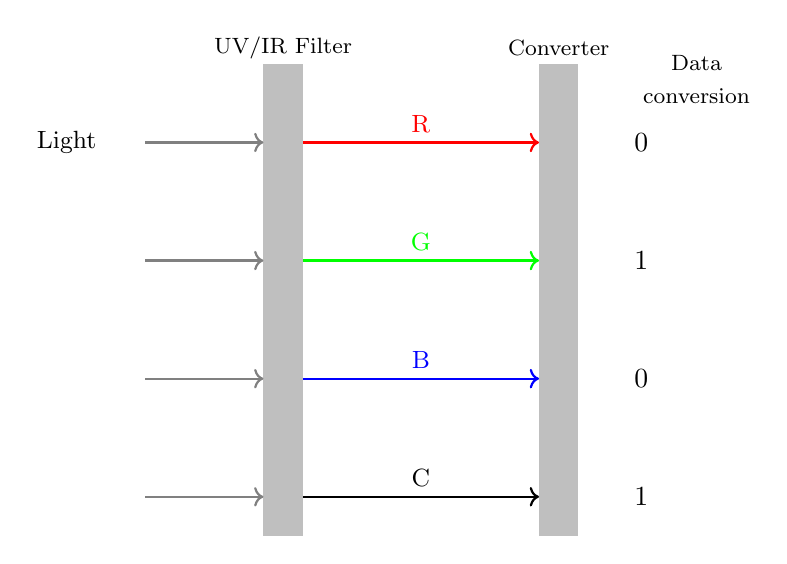
\begin{tikzpicture}
		
		% UV/IR Filter and Converter rectangles
		\fill[gray!50] (2, -2.5) rectangle (2.5, 3.5);
		\fill[gray!50] (5.5, -2.5) rectangle (6, 3.5);
		
		% Labels
		\node at (-0.5, 2.5) {\small Light};
		\node at (2.25, 3.7) {\footnotesize UV/IR Filter};
		\node at (5.75, 3.7) {\footnotesize Converter};
		\node[align=center] at (7.5, 3.3) {\footnotesize Data \\ \footnotesize conversion};
		
		% Arrows for light input
		\draw[->, thick, gray] (0.5, 2.5) -- (2, 2.5);
		\draw[->, thick, gray] (0.5, 1) -- (2, 1);
		\draw[->, thick, gray] (0.5, -0.5) -- (2, -0.5);
		\draw[->, thick, gray] (0.5, -2) -- (2, -2);
		
		% Color-coded arrows
		\draw[->, thick, red] (2.5, 2.5) -- (5.5, 2.5) node[midway, above] {\small R};
		\draw[->, thick, green] (2.5, 1) -- (5.5, 1) node[midway, above] {\small G};
		\draw[->, thick, blue] (2.5, -0.5) -- (5.5, -0.5) node[midway, above] {\small B};
		\draw[->, thick, black] (2.5, -2) -- (5.5, -2) node[midway, above] {\small C};
		
		% Data conversion outputs
		\node at (6.8, 2.5) {0};
		\node at (6.8, 1) {1};
		\node at (6.8, -0.5) {0};
		\node at (6.8, -2) {1};
	\end{tikzpicture}
	
	\captionof{figure}{Schematic of the main function of a color sensor}
	\label{fig:SchematicColorSensor}
\end{center}

The block diagram \ref{fig:FunctionalBlockDiagram} shows the processing flow of the APDS-9660 from light detection to communication via the I²C protocol with the Arduino. The individual steps are explained as follows:

\tikzstyle{block} = [rectangle, draw, minimum width=3.5cm, minimum height=1.2cm, text centered, text width=3.5cm]
\tikzstyle{smallblock} = [rectangle, draw, minimum width=3.5cm, minimum height=1.2cm, text centered]
\tikzstyle{arrow} = [thick,->,>=stealth]
\tikzstyle{sensor} = [draw, isosceles triangle, isosceles triangle apex angle=60, shape border rotate=-90, minimum height=1.5cm, minimum width=1.5cm, text centered]

\begin{center}
	\begin{tikzpicture}[node distance=2.5cm, scale=0.5, every node/.style={transform shape}]
		
		% Sensors
		\node (clear) [sensor] {Clear};
		\node (red) [sensor, below of=clear] {Red};
		\node (green) [sensor, below of=red] {Green};
		\node (blue) [sensor, below of=green] {Blue};
		
		% RGBC + ALS
		\node (rgbc_als) [block, right of=red, xshift=3cm] {RGBC \\ ALS};
		
		% MUX
		\node (mux) [smallblock, right of=rgbc_als, xshift=3cm] {MUX};
		
		% ADC
		\node (adc) [smallblock, right of=mux, xshift=3cm] {ADC};
		
		% FIFO + Threshold Control
		\node (fifo) [block, right of=adc, xshift=3.5cm] {32 x 4 Byte FIFO \\ Threshold Control};
		
		% I2C Interface
		\node (i2c) [block, above of=fifo, yshift=2cm] {I\textsuperscript{2}C Interface};
		
		% Interrupt
		\node (interrupt) [smallblock, below of=fifo, yshift=-2cm] {Interrupt};
		
		% Connections
		\draw [arrow] (clear) -- (rgbc_als);
		\draw [arrow] (red) -- (rgbc_als);
		\draw [arrow] (green) -- (rgbc_als);
		\draw [arrow] (blue) -- (rgbc_als);
		\draw [arrow] (rgbc_als) -- (mux);
		\draw [arrow] (mux) -- (adc);
		\draw [arrow] (adc) -- (fifo);
		\draw [arrow] (fifo) -- (i2c);
		\draw [arrow] (fifo) -- (interrupt);
		\draw [arrow] (i2c) -- ++(2.5cm,0) node[right] {SCL};
		\draw [arrow] (i2c) -- ++(2.5cm,-1.5cm) node[right] {SDA};
		\draw [arrow] (interrupt) -- ++(2.5cm,0) node[right] {INT};
		
	\end{tikzpicture}
	
	\captionof{figure}{Functional Block Diagram}
	\label{fig:FunctionalBlockDiagram}
\end{center}

\Mynote{The graphic is not optimal. Description of the individual blocks is not clear. What does RGBC and ALS mean?}


The photodiodes convert the intensities of the color components of the filtered light and the total light into electrical signals.
These RGBC (Red, Green, Blue, Clear) and ALS (Ambient Light Sensor) signals are forwarded to the next processing stage using the multiplexer (MUX). 

The MUX allows for the sequential processing of the color signals, as the ADC (Analog-to-Digital Converter) can only process one signal at a time.
The ADC converts the analog signal selected by the MUX into a digital value. This conversion is necessary to make the signal suitable for digital processing and transmission.

The digital value is stored in a FIFO (First In, First Out) data register, which can store up to 32 data values (4 bytes each). A threshold controller monitors the data and triggers an interrupt when defined limits are reached. The detailed process is explained in Chapter Data Processing \ref{chap:Data Processing}.

The stored data is transmitted to the Arduino via an I²C bus. The I²C bus uses two lines: the SCL (Serial Clock Line) for the clock and the SDA (Serial Data Line) for data transmission. The detailed functioning of the I²C bus is explained in Chapter \ref{chap:Protokoll I²C} Protokoll I²C.
\cite{Avago:2015}.

\subsubsection{Data Processing}
\label{chap:Data Processing}

The color detection begins at the photodiodes with RGBC detection and ends with 16-bit values stored in the RGBC data registers. The signal from the photodiode array is accumulated over a period defined by the value in the ATIME register (ALS ADC Integration Time) before the results are transferred to the RGBCDATA registers. The gain factor can be set from 1x to 64x, which is controlled via the CONTROL<AGAIN> bit (ALS Gain Control). Performance parameters such as accuracy, resolution, conversion speed, and energy consumption can be adjusted to meet the application requirements.

Between measurements, a customizable, energy-efficient waiting period is maintained, the duration of which is determined by the control bits WEN (Wait Enable), WTIME (Wait Time), and WLONG (Wait Long Enable). The waiting time can range from 0 seconds to a maximum of 8.54 seconds.

An interrupt is triggered when the clear channel values exceed the thresholds defined in the AILTL/AIHTL (ALS low threshold, lower byte/ALS high threshold, lower byte) or AILTH/AIHTH (ALS low threshold, upper byte/ALS high threshold, upper byte) threshold registers. To avoid unwanted or false interrupts, a persistence filter is integrated, ensuring that an interrupt is triggered only when a defined number of consecutive values fall outside the thresholds. This threshold is set in the APERS register (ALS Interrupt Persistence). If a value is within the thresholds, the persistence counter is reset. If the analog circuit is saturated, the ASAT bit is set, indicating potentially inaccurate RGBCDATA results. The AINT (ALS Interrupt) and CPSAT (Clear Diode Saturation) bits can be queried at any time via I²C. However, for AINT to trigger a hardware interrupt on the INT pin, the AIEN bit (ALS Interrupt Enable) must be set. Saturation of the analog-to-digital converter can be detected via the CPSAT bit; to enable this function, the CPSIEN bit (Clear Diode Saturation Interrupt Enable) must be set. The AVALID bit (ALS Valid) is reset by reading the RGBCDATA. ASAT and AINT can be reset via the CICLEAR (Clear Channel Interrupt Clear) or AICLEAR (All Non-Gesture Interrupt Clear) bits.

The RGBC results can be used to determine the color temperature in Kelvin or the ambient light intensity in Lux.

\cite{Avago:2015}








\section{Specific Sensor}

cite board

\section{Specification}

\begin{itemize}
  \item cite data sheet
  \item Circuit Diagram
\end{itemize}

\section{Bibliothek}

\subsection{Description}

\subsection{Installation}

\subsection{Functions}

\subsection{Example - Manual}

\subsection{Example}

\subsection{Example - Code}

\subsection{Example - Files}



\section{Calibration}

cite method

\section{Simple Code}


\section{Simple Application}



\section{Tests}

\subsection{Simple Function Test}

\subsection{Test all Functions}

\section{Simple Application}


\section{Further Readings}


 % %%%%%%%%%%%%
%
% $Autor: Wings $
% $Datum: 2019-03-05 08:03:15Z $
% $Pfad: TemplateSensor $
% $Version: 4250 $
% !TeX spellcheck = en_GB/de_DE
% !TeX encoding = utf8
% !TeX root = filename 
% !TeX TXS-program:bibliography = txs:///biber
%
%%%%%%%%%%%%

% Structure
\chapter{Sensor APDS 9960 Proximity}

The proximity sensor is part of the gesture detection sensor and detects top-bottom gestures based on the temporal change in the measured distance. The proximity detection measures the distance between the sensor and an object by capturing the reflected IR light. The integrated IR LED emits light, which is measured by the same photodiodes as in gesture detection. The stronger the reflection, the closer the object is. The proximity sensor can also detect events such as the approach or withdrawal of an object and trigger corresponding interrupts when predefined thresholds are exceeded. To ensure reliable measurements, the sensor compensates for unwanted reflections by adjusting offset values and suppresses interference from ambient light.
\smallskip
\cite{Avago:2015}



\section{General}

General description

cite books

\section{Specific Sensor}

cite board

\section{Specification}

\begin{itemize}
  \item cite data sheet
  \item Circuit Diagram
\end{itemize}

\section{Bibliothek}

\subsection{Description}

\subsection{Installation}

\subsection{Functions}

\subsection{Example - Manual}

\subsection{Example}

\subsection{Example - Code}

\subsection{Example - Files}



\section{Calibration}

cite method

\section{Simple Code}


\section{Simple Application}



\section{Tests}

\subsection{Simple Function Test}

\subsection{Test all Functions}

\section{Simple Application}


\section{Further Readings}


 % %%%%%%%%%%%%
%
% $Autor: Wings $
% $Datum: 2019-03-05 08:03:15Z $
% $Pfad: TemplateSensor $
% $Version: 4250 $
% !TeX spellcheck = en_GB/de_DE
% !TeX encoding = utf8
% !TeX root = filename 
% !TeX TXS-program:bibliography = txs:///biber
%
%%%%%%%%%%%%

% Structure
\chapter{Sensor Ambient Light}

The ambient light sensor (ALS) of the APDS-9960 works with the same photodiode array and measures the intensity of the ambient light. For this purpose, the UV and IR light filters are installed in front of the photodiodes to ensure accurate measurements of visible light. The sensor converts the measured light intensity into 16-bit data, which enables high resolution and accuracy. A function of programmable gain and customizable integration time ensures that the sensor can operate accurately in different lighting conditions, such as dim or very bright light.
\medskip
Another important feature of the sensor is its ability to correctly detect the intensity of ambient light even behind dark glass, which is particularly useful for devices with tinted covers.
\smallskip
\cite{Avago:2015}


\section{General}

General description

cite books

\section{Specific Sensor}

cite board

\section{Specification}

\begin{itemize}
  \item cite data sheet
  \item Circuit Diagram
\end{itemize}

\section{Bibliothek}

\subsection{Description}

\subsection{Installation}

\subsection{Functions}

\subsection{Example - Manual}

\subsection{Example}

\subsection{Example - Code}

\subsection{Example - Files}



\section{Calibration}

cite method

\section{Simple Code}


\section{Simple Application}



\section{Tests}

\subsection{Simple Function Test}

\subsection{Test all Functions}

\section{Simple Application}


\section{Further Readings}



 % \InputLanguage{Contents/General/}{AppADPS9960}

 % \InputLanguage{Contents/General/}{MicrophoneMP34DT05}

  \InputLanguage{Contents/General/}{IMU}
  \input{../../Contents/General/IMUSoftware}
  \input{../../Contents/General/IMUCalibration}
  \input{../../Contents/General/IMUErrors}
  \input{../../Contents/General/IMULibFunctions}
  %%%
%
% $Autor: Wings $
% $Date: 2024-10-31 11:15:45Z $
% $File: AccelerationDetectionAlgorithms.tex $
% $Version: 1 $
%
%%%


\chapter{Distance,  Speed and Acceleration Detection Algorithms}

\section{Review of Distance Measurement Methods}

Since Mitsubishi released the first cruise control with distance control in 1995, the vast majority of ACC functions have been based on Laser Radar or millimeter-wave radar (MWR). \footnote{MI-PILOT, Mitsubishi Motors, \url{https://www.mitsubishi-motors.com/en/brand/technology/mipilot2/index.html}} But a few have opted to use a binocular camera as the basis for the technology, such as Subaru's EyeSight technology. \footnote{EyeSight technology, Subaru, \url{https://www.subaru.com/eyesight.html}}

Each of these different sets of technical solutions has its own advantages and disadvantages:

\begin{table}[h]
	\centering
	\resizebox{\textwidth}{!}{
		\begin{tabular}{|p{3cm}|p{6cm}|p{6cm}|}
			\hline
			\textbf{Technology} & \textbf{Advantages} & \textbf{Disadvantages} \\ \hline
			\textbf{Laser Radar (LiDAR)} & 
			\begin{tabular}[c]{@{}p{6cm}@{}}
				- High accuracy and resolution \\
				- Capable of creating detailed 3D maps \\
				- Effective for object detection and classification
			\end{tabular} &
			\begin{tabular}[c]{@{}p{6cm}@{}}
				- Expensive \\
				- Affected by adverse weather conditions \\
				- High power consumption
			\end{tabular} \\ \hline
			
			\textbf{Millimeter-Wave Radar} &
			\begin{tabular}[c]{@{}p{6cm}@{}}
				- Less affected by weather conditions \\
				- Long-range detection capabilities \\
				- Lower cost compared to LiDAR
			\end{tabular} &
			\begin{tabular}[c]{@{}p{6cm}@{}}
				- Lower resolution than LiDAR \\
				- Limited in detecting small or non-metallic objects \\
				- Can be affected by interference
			\end{tabular} \\ \hline
			
			\textbf{Binocular Camera Systems} &
			\begin{tabular}[c]{@{}p{6cm}@{}}
				- Lower cost compared to LiDAR and radar \\
				- High resolution for nearby objects \\
				- Uses passive sensing (no emissions)
			\end{tabular} &
			\begin{tabular}[c]{@{}p{6cm}@{}}
				- Computationally intensive \\
				- Accuracy decreases with distance \\
				- Affected by lighting conditions
			\end{tabular} \\ \hline
		\end{tabular}
	}
	\caption{Comparison of distance measurement technologies: LiDAR, Millimeter-Wave Radar, and Binocular Cameras}
	\label{tab:comparison}
\end{table}

For cars using Laser Radar, LiDAR operates by emitting laser pulses towards objects in front of the vehicle. When these pulses hit an object, they are reflected back to the sensor, which measures the time it takes for the pulses to return. This time-of-flight measurement allows the system to calculate the precise distance to the object, as well as its relative speed and position. For cars using millimeter-wave radar, the functional implementation is similar.

For systems that use binocular cameras, this process can be relatively more complex; essentially distance recognition for binocular camera-based systems utilizes bionics: Binocular disparity. This method involves using a pair of cameras positioned at a certain distance apart to capture two images with different viewing angles. By comparing the disparity between the two images (i.e., the difference in pixel positions).\footnote{Mansour, M., Davidson, P., Stepanov, O. and Piché, R., 2019. Relative Importance of Binocular Disparity and Motion Parallax for Depth Estimation: A Computer Vision Approach. Remote Sensing, 11(17), p.1990. \url{https://doi.org/10.3390/rs11171990}}

\begin{equation}
	\text{depth} = \frac{f \times \text{baseline}}{\text{disparity}}
\end{equation}

where depth represents the distance of an object from the camera, f denotes the focal length of the camera, baseline is the distance between the two cameras, and disparity is the difference in image location of the object in the two camera views.

\begin{figure}[H]
	\centering
	\begin{minipage}{1\textwidth}
		\centering
		\includegraphics[width= 0.75\linewidth]{AccelerationDetectionAlgorithms/Baseline.png}
		\caption{Design of OAK-D Pro camera}
	\end{minipage}
\end{figure}

For the OAK-D Pro camera, the baseline distance, which is the distance between the two monochrome cameras, is 7.5 cm. \footnote{OAK-D Pro Camera Documentation, Luxonis, 2021}

According to OAK's official documentation\footnote{OAK China official Website, OAK China, 2024}, the OAK-D Pro can reach a theoretical maximum of 35m, but at this distance there is a very significant margin of error (about 33\% of the theoretical error\footnote{Depth range enhancement, Luxonis Community, 2022}) where the distance fluctuates very significantly. However, there are ways to improve the accuracy of distance detection, such as half-pixel mode to improve the accuracy of distance detection, and averaging distances over a period of time to calculate relative distances to improve the accuracy of relative speed calculations.


\section{Review of Speed and Acceleration Detection Algorithms}

For the measurement of relative velocity, the three schemes mentioned above will actually have two different principles and calculations.

Millimeter-wave radar primarily calculates the relative speed of objects using the Doppler effect. When the radar signal hits a moving object, the frequency of the reflected wave changes depending on the relative speed between the radar and the object. This frequency shift (Doppler shift) is directly proportional to the relative speed of the object. \footnote{Millimeter Wave Radar Sensors: Fundamentals, Texas Instruments, 2018}

For LiDAR and Binocular Camera Systems, the relative speed of objects is calculated based on the change in distance over time. By continuously measuring the distance to an object and comparing it with previous measurements.

Each of these different sets of technical solutions has its own advantages and disadvantages:

\begin{table}[h]
	\centering
	\resizebox{\textwidth}{!}{
		\begin{tabular}{|p{3cm}|p{6cm}|p{6cm}|}
			\hline
			\textbf{Technology} & \textbf{Advantages} & \textbf{Disadvantages} \\ \hline
			\textbf{Laser Radar (LiDAR)} & 
			\begin{tabular}[c]{@{}p{6cm}@{}}
				- High accuracy and resolution \\
				- Capable of creating detailed 3D maps \\
				- Effective for object detection and classification
			\end{tabular} &
			\begin{tabular}[c]{@{}p{6cm}@{}}
				- Expensive \\
				- Affected by adverse weather conditions \\
				- High power consumption
			\end{tabular} \\ \hline
			
			\textbf{Millimeter-Wave Radar} &
			\begin{tabular}[c]{@{}p{6cm}@{}}
				- Less affected by weather conditions \\
				- Long-range detection capabilities \\
				- Lower cost compared to LiDAR
			\end{tabular} &
			\begin{tabular}[c]{@{}p{6cm}@{}}
				- Lower resolution than LiDAR \\
				- Limited in detecting small or non-metallic objects \\
				- Can be affected by interference
			\end{tabular} \\ \hline
			
			\textbf{Binocular Camera Systems} &
			\begin{tabular}[c]{@{}p{6cm}@{}}
				- Lower cost compared to LiDAR and radar \\
				- High resolution for nearby objects \\
				- Uses passive sensing (no emissions)
			\end{tabular} &
			\begin{tabular}[c]{@{}p{6cm}@{}}
				- Computationally intensive \\
				- Accuracy decreases with distance \\
				- Affected by lighting conditions
			\end{tabular} \\ \hline
		\end{tabular}
	}
	\caption{Comparison of distance measurement technologies: LiDAR, Millimeter-Wave Radar, and Binocular Cameras}
	\label{tab:comparison}
\end{table}




}


%\Ausblenden
{

\part{Arduino Nano 33 BLE Sense - External  Sensors and Actors}

  \input{../../Contents/Nano33BLESense/TinyMLKit}

  %%%%%%%%%%%%%%%
%
% $Autor: Wings $
% $Datum: 2020-01-29 07:55:27Z $
% $Pfad: General/PowerTinyMLShield.tex
% $Version: 1785 $
%
%
%%%%%%%%%%%%%%%

%source: https://projecthub.arduino.cc/paulsb/temp-and-humidity-monitor-with-graphs-and-battery-monitor-cd011a

% https://www.az-delivery.de/products/az-delivery-laderegler-tp4056-mini-usb?variant=12239811084384
%https://www.az-delivery.de/products/cd60l-batterieladecontroller
%https://www.az-delivery.de/products/mini-solarpanel?variant=39475872792672

    
\chapter{Powering the TinyML Shield}

Now that you have your Arduino development board up and running, let's talk about how you could deploy it independent of your computer! While some embedded systems call on AC-DC converters (or “wall warts,” colloquially) to provide low voltage power to their electronics (the Google home speaker, for example), others are battery powered. Both of these paradigms are applicable to real-world deployment of tinyML and both are achievable using your TinyML kit.

\Mynote{Komplettes Kapitel muss überarbeitet werden. Sortierung, Quellen, Diagramm,\ldots}
\subsection{USB Power Delivery}

To this point, we have provided power over USB to our microcontroller via the microB port on the Nano 33 BLE Sense. The 5V that USB carries is then down regulated on the development board to 3.3V, the logical reference for the MCU. While there’s nothing wrong with this in development, a prototype of your application ought not depend on drawing power from your computer. Instead, you could call on an AC-DC converter with USB output. This has the added benefit of likely raising the current capacity of the 5V power rail, from at most 500 mA via a computer to whatever the specification happens to be for a given wall-bound converter. This could be meaningful for driving certain power hungry actuators, like speakers.

\section{Battery}

While the above solution removes the need for the computer, you’re still tethered to a wall. To go fully mobile you’ll want to call on a battery. So what are our options? The idea of using a voltage regulator (specifically, the MPM3610) to cut down an input voltage to a nice, stable 3.3V level applies here as well. If you were to take a closer look at the linked datasheet, you’d find that the MPM3610 accepts input voltages from 4.5V to 21V. The 5V delivered over USB is within this range, and any compatible battery will need to be as well. This unfortunately eliminates the possibility of calling on single cell 3.7V lithium batteries, but makes the selection of a 9V alkaline battery fairly obvious.

You might be wondering how any battery might connect to the boards in front of you, but never fear, we’ve got you covered. At one corner of the Tiny Machine Learning Shield you’ll find a green terminal block with silkscreen labels that read, “VIN” and “GND,” where GND is our reference voltage and as such should be connected to the negative terminal of any compatible battery. This green terminal block is where you’d want to screw in wires carrying 4.5V to 21V, and we’ll add that 9V clip, like this, that terminates in pre-stripped hook-up wire makes this quite easy!

\bigskip

Assembly Steps

\begin{enumerate}
    \item Screw down a wire leading from the negative battery terminal (black) to GND (Most < 3mm flat-head screwdrivers will suffice here).
    \item Repeat this process for the positive battery terminal (red) to VIN. And that's it you're all set to power your Arduino from a battery!
\end{enumerate}


\bigskip

Important Notes

\begin{enumerate}
    \item While there is clever circuitry on board to handle such an exception, it is generally good practice to avoid having competing power sources, so we’d recommend that you unplug the Nano 33 BLE Sense from USB power before connecting a battery
    
    \item With about 550 mAh capacity, a 9V battery can source 15 mA for about 37 hours before you will need to get a new one.
\end{enumerate}


\Mynote{tikz-Bild des Shields fehlt.}

\medskip

\begin{center}
  \includegraphics[width=\textwidth]{Battery/batteryScrew.png}
  \captionof{figure}{Montage des Clips}
\end{center}


An image of screwing down the black negative terminal to attach a wire.

\begin{center}
  \includegraphics[width=\textwidth]{Battery/batteryDone.png}
  \captionof{figure}{Komplettes System mit Batterie}
\end{center}

An image of the attached battery powering the device.


\section{Checking the Battery Voltage}

We use an analog input pin to read the voltage. As we are running from a 3.7V volt battery, we need to adjust the reference voltage used by the pin as otherwise it would be comparing the voltage to itself. The statement \PYTHON{analogReference(INTERNAL)} sets the pin to compare the input voltage to a regulated 1.1V. We therefore need to reduce the voltage on the input pin to less than 1.1V for this to work. This is done by dividing the voltage using 2 resistors, 1m and 330k ohms. This divides the voltage by approximately 4 so when the battery is fully charged, which is 4.2V, the voltage at the pin input is 4.2/4 = 1.05V. 

\begin{lstlisting}[language=python]
// Battery Monitor
#define MONITOR_PIN  A0              // Pin used to monitor supply voltage
const float voltageDivider  = 4.0;   // Used to calculate the actual voltage fRom the monitor pin reading
                                     // Using 1m and 330k ohm resistors divids the  voltage by approx 4
                                     // You may wany to substitute  actual values of resistors in an equation (R1 + R2)/R2
                                     // E.g. (1000 + 330)/330 = 4.03
                                     // Alternatively  take the voltage reading across the battery and from the joint between 
                                     //  the 2 resistors to ground and divide one by the other to get the value.
    
// Read the monitor pin and calculate the voltage 
float BatteryVoltage()
{ 
    float reading = analogRead(MONITOR_PIN); 
    // Calculate voltage - reference voltage is 1.1v 
    return 1.1 * (reading/1023) * voltageDivider; 
} 
\end{lstlisting}

The function \PYTHON{BatterVoltage()}, reads the analog pin, which will range from 0 for 0V to 1,023 for 1.1V and using this reading calculates the actual voltage coming form the battery. 

The function \PYTHON{DrawScreenSave()} function calls this then selects the appropriate bitmap to display based on the following: 

\begin{itemize}
    \item If voltage is greater then 3.6V - full 
    \item Voltage between 3.5 and 3.6V - 3/4 
    \item Voltage between 3.4 and 3.5V - half 
    \item Voltage between 3.3 and 3.4V - 1/4 
    \item Voltage < 3.3V - empty 
\end{itemize}



\section{Batterieclip}

Der Batterieclip in Abb. \ref{Batterieclip für 9-Volt-Block}, der vom Hersteller \textit{reichelt} ist, kann vertikal an einen 9-Volt-Block angeschlossen werden. Die dazugehörigen Anschlussdrähte haben eine Länge von 150 mm. Der Anschlussclip ist in der I-Form ausgeführt, weshalb er sich platzsparend ins Gehäuse einbinden lässt \cite{Reichelt:2011}.

\begin{figure}[h]
    \begin{center}
        \includegraphics[width=3in]{Battery/clip.jpg}
        \caption{Batterieclip für 9-Volt-Block\cite{Reichelt:2024a}}
        \label{Batterieclip für 9-Volt-Block}
    \end{center}
\end{figure} 



\section{Spannungssensor}

Der Spannungssensor in Abb. \ref{Spannungssensor} von dem Hersteller \textit{Shenzhen Global Technology Co., Ltd} kann bei der Versorgungsspannung von 3,3 V Spannungen in dem Bereich von 0 V bis 16,5 V messen. Dieser wird genutzt, um den Ladestand der Batterie zu überwachen. Die analoge Auflösung des Sensors liegt bei 10 Bit. Damit kann bei dem angegebenen Messbereich die Spannung mit der Auflösung von 0,016 V gemessen werden. Zur Eingangsschnittstelle gehört der \ac{vcc}-Anschluss und der \ac{gnd}-Anschluss \cite{Shenzhen:2015}. Die Bauteilmaße betragen 13 mm x 27 mm.



{\begin{center}
		
  \includegraphics[width=0.6\textwidth]{Battery/VoltageSensor}
  
  \captionof{figure}{Voltage Sensor 170640  von dem Hersteller \textit{Shenzhen Global Technology Co., Ltd}\cite{Shenzhen:2015}}   		
		
	\end{center}
}
	
Mit dem Sketch \FILE{TestBattery.ino}, siehe \ref~{TestBattery}, soll der Spannungssensor getestet werden.

\medskip



\begin{code}
	
	\caption{Beispiel-Sketch zum Testen der Batterie}\label{TestBattery}

    \ArduinoExternal{}{../../Code/Arduino/Battery/TestBattery.ino}
\end{code}

\subsection{Durchführung}

Für den Test werden die folgenden Hardware-Komponenten benötigt:

\begin{itemize}
    \item Arduino Nano 33 BLE Sense Lite
    \item Tiny Machine Learning Shield
    \item USB-A auf USB-Mikro Verbindungskabel
    \item Grove Jumper zu Grove 4 Pin Kabel
    \item Spannungssensor
    \item Batterie
    \item Batterieclip
\end{itemize}

Die Hardware-Komponenten werden  zusammengebaut, aber die Batterie wird noch nicht angeschlossen. Dann wird der Arduino Nano 33 BLE Sense Lite mit einem Computer verbunden. Anschließend wird der Sketch \FILE{TestBattery.ino} auf den Arduino Nano 33 BLE Sense Lite geladen und der serielle Monitor in der Arduino \acs{ide} geöffnet. Die Batterie wird während des Tests an den Batterieclip angeschlossen und der gemessene Wert bei dem seriellen Monitor ausgelesen.

\subsection{Ergebnisse}

Zu Beginn des Tests zeigt der serielle Monitor die Spannung 0 V an. Nach dem Anschließen der Batterie an den Spannungssensor wird die Spannung 9,6 V angezeigt.  Abbildung~\ref{BildSpannungTest} zeigt den gemessenen Spannungsverlauf. Die angezeigte Spannung liegt in dem erwarteten Bereich einer 9 V Batterie.

\begin{figure}[h]
    \begin{center}
        \includegraphics[width=\textwidth]{Battery/BatteryTest.png}
        \caption{Testoutput des Spannungssensors}
        \label{BildSpannungTest}
    \end{center}
\end{figure}



  %%%%%%%%%%%%
%
% $Autor: Wings $
% $Datum: 2019-03-05 08:03:15Z $
% $Pfad: PushButton $
% $Version: 4250 $
% !TeX spellcheck = en_GB/de_DE
% !TeX encoding = utf8
% !TeX root = filename 
% !TeX TXS-program:bibliography = txs:///biber
%
%%%%%%%%%%%%

% Structure
\chapter{TinyML Shield: Built-in Push Button}\index{Push Button! Built-in Push Button}

\section{General}

A push button is a simple switch mechanism used to control various devices and processes. It is typically made of hard materials like plastic or metal.
The surface of a push button is designed to be easily depressed or pushed by the human finger or hand. When you press a push button, it either closes or opens an electrical circuit. 

In industrial and commercial applications, push buttons can be linked together so that pressing one button releases another. Emergency stop buttons, often with large mushroom-shaped heads, enhance safety in machines and equipment. Pilot lights are sometimes added to push buttons to draw attention and provide feedback when the button is pressed. Color-coding is common to associate push buttons with their specific functions (e.g., red for stopping, green for starting). \cite{DIN:13850}

%\Mynote{cite books, applications, board\\ image of the board}






\section{Built-in Push Button}

The Arduino Nano 33 BLE Sense features an onboard push button. This button is a simple electrical switch that can be activated by pressing it. When you press the button, it completes an electrical circuit. The push button is designed for user interaction and can be used for various purposes.

The built-in button \PYTHON{BUTTON\_B} is connected with pin 11.\index{Pin!Pin 11} Using the function \PYTHON{pinMode(BUTTON\_PIN, INPUT\_PULLUP)} the pin is declared as an input. As can be seen in the sketch, pressing the button can be used to trigger actions; typical actions include switching on an LED, changing modes, or initiating sensor readings.
Overall, the push button provides a convenient way to interact with the Arduino Nano 33 BLE Sense and create responsive projects. \cite{Arduino:2023a,Arduino:2023,ArduinoNano33Manual:2022}


\bigskip


\Mynote{Push Button hier nochmal mit tikz-code hervorheben}

\begin{center}
	
	\begin{tikzpicture}
		\ArduinoNanoShieldTikz
	\end{tikzpicture}    
	
	%  \includegraphics[width=0.9\textwidth]{Nano33BLESense/TinyMLKit/TinyMachineLearningShieldRotated.png}
	\captionof{figure}[The Tiny Machine Learning Shield]{ Tiny Machine Learning Shield \cite{ArduinoShield:2021}}
\end{center}






\Ausblenden{arg1


\begin{center}    
    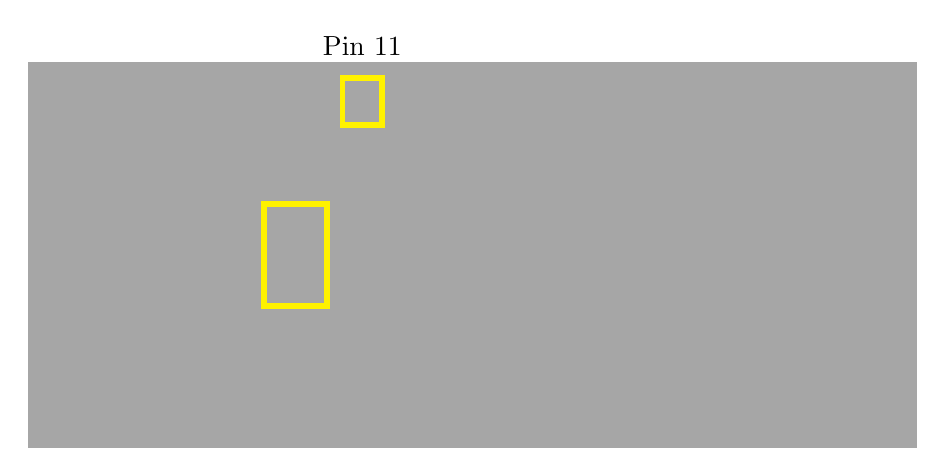
\begin{tikzpicture}
        %\node at (0,0) (Board) {\includegraphics{Arduino/Nano33BLE/Nano33BLESense}};
        
        \ArduinoNanoTikz;
        
        \fill[gray, opacity=0.7] (-11.2,-0.2) rectangle (0.1,4.7);
        
        \coordinate (A) at (-8.2,1.6);
        \coordinate (B) at (-7.4,2.9); 
        
        
        \coordinate (C) at (-7.2,3.9);
        \coordinate (D) at (-6.7,4.5);  
        
        \def\cliparea{(C) rectangle (D); (A) rectangle (B); }  
        
        \begin{scope}
            \clip (A) rectangle (B);
            
            \ArduinoNanoTikz
            
            %\node at (0,0) (Board) {\includegraphics{Arduino/Nano33BLE/Nano33BLESense}};
            
        \end{scope}
        
        %        \fill[ArduinoColor] (C) rectangle (D);
        %         \fill[gray!30] ({-8.16-0.195},4.145) rectangle ++(0.39, 0.39); 
        %        \draw[fill=gray!30,gray!30] (-8.145,4.143) circle(0.195); 
        %        \draw[fill=gray!60,gray!60] (-8.145,4.143) circle(0.165); 
        %        \fill[white,white](-8.145,{4.143+0.39}) circle (0.1275);
        
        \draw[yellow,line width=2pt] (A)  rectangle (B);
        \draw[yellow,line width=2pt] (C)  rectangle (D);
        
        \node (P25) at (-6.95, 4.9) {Pin 11};
    \end{tikzpicture}    
    
    
    
    \captionof{figure}{Arduino Nano 33 BLE Sense's built-in Push Button  with Pin 11}  
\end{center}

}






\section{Specification}

The built-in button is a small white button  and connected to pin 11.\index{Pin!Pin 11}

\begin{description}
    \item [Built-in Button:] \PYTHON{BUTTON\_B =  11u}
\end{description}

If the pin is declared as input in the function \PYTHON{setup}, then it can be used.

%\Mynote{cite data sheet, power consumption?}

The pin 11 must be defined as an input in the function \PYTHON{setup} by setting \PYTHON{pinMode (11, INPUT\_PULLUP)}, otherwise the button cannot be read.

\medskip 


The pin 11 can also be used otherwise. Then the button is not in use. \cite{Arduino:2023a,Arduino:2023,ArduinoNano33Manual:2022}

%\Mynote{What happen if there is another button at the pin? Both in use?}

\Mynote
{
\begin{itemize}
  \item cite data sheet
  \item Circuit Diagram
\end{itemize}
}

\section{Simple Code}


As soon as the button is connected, it can be used. It is not necessary to install a special library. Programming takes place in two steps:

\begin{enumerate}
    \item In the first step, the pin is configured in the function \PYTHON{setup}:
    
    {
        \captionof{code}{Defining the built-in button's pin as an input.}
        \begin{Arduino}
            pinMode(BUTTON_B, INPUT_PULLUP)   
        \end{Arduino}
    }
    \item In the second step, the button can be used in the function \PYTHON{loop}. To read in the value, use the function \PYTHON{digitalRead}:
    
    {
        \captionof{code}{Read the built-in button's state}
        \begin{Arduino}
            buttonState = digitalRead(BUTTON_B);
        \end{Arduino}
    }
    
\end{enumerate}




\section{Tests}


The simplest test is the flashing of an LED for 2 seconds, if the button is pressed, see sketch \ref{Nano:BuiltinButtonTest}.

{
    \captionof{code}{Simple sketch to test the push button and the built-in LED}\label{Nano:BuiltinButtonTest}
    \ArduinoExternal{}{../../Code/Nano33BLESense/PushButton/TestPushButton/TestPushButton.ino}
}

\section{Interrupt Function on the Arduino Nano 33 BLE Sense}


An interrupt is a function that allows the microcontroller on the Arduino Nano 33 BLE Sense to immediately respond to an external event, such as pressing a button, without the need for the program to continuously check for that event. Normally, in a program, the microcontroller would repeatedly check if a button is pressed by running through a loop, which consumes processing power and can slow down other tasks. This is not efficient, especially when the program needs to perform other actions at the same time.

With an interrupt, the program can continue running other tasks, and only when the specified event (like a button press) occurs, the program is temporarily paused to execute a special function known as the \menu{Interrupt Service Routine (ISR)}. The ISR is a small, efficient function designed to handle the event, such as changing a variable or triggering another action. After the ISR is executed, the program returns to where it left off, continuing its normal operation.

Using interrupts in this way helps make the program more efficient and responsive, as it doesn't waste time constantly checking for events and can focus on other tasks until something important happens. This is especially useful for real-time applications where quick responses to external events are necessary, such as in embedded systems, robotics, or sensor monitoring.



\section{Simple Application}



This code sketch \ref{Nano:TestButtonInterrupt} shows how to use an interrupt to control the built-in LED on the Arduino Nano 33 BLE Sense when the built-in push button is pressed.

The program sets up the built-in LED and push button. When the button is pressed, an interrupt runs a special function called an Interrupt Service Routine. The ISR is very short and only sets a flag variable \PYTHON{pushPressed} to \PYTHON{true}, indicating that the button has been pressed.

The main program \PYTHON{loop} checks this flag. If it is set to \PYTHON{true}, the program turns on the LED for 2 seconds, then turns it off and resets the flag to \PYTHON{false}. This ensures the system is ready to detect the next button press. Using the \PYTHON{true and false} values makes it easy to manage the button's state.

This method avoids constantly checking the button’s state, making the program more efficient. Additionally, the Arduino Nano 33 BLE Sense allows all its pins to be used for interrupts. This makes it easy to attach interrupt functions to any pin, allowing quick and efficient responses to inputs like buttons or sensors. \cite{ArduinoInterrupt:2019}


\Mynote{andere Überschrift für simple Application}

\bigskip







{
    \captionof{code}[Simple sketch connects the push button with an interrupt.]{Simple sketch connects the push button with an interrupt. Here, pushing the built-in button is handled by an interrupt. Then the built-in LED switch on for 2 sec.}\label{Nano:TestButtonInterrupt}
    \ArduinoExternal{}{../../Code/Nano33BLESense/PushButton/TestPushButtonInterrupt/TestPushButtonInterrupt.ino}
}

\bigskip

This is just a simple example. The variable \PYTHON{BUTTON\_B} is already defined, so the assignment is not necessary. The command \PYTHON{delay} should be avoided in an Arduino sketch. Instead, variables of the type \PYTHON{elapsedMillis} should be used.



\section{Further Readings}

\begin{itemize}
  \item Boxall, John: \textsl{Arduino Workshop - A Hands-On Introduction with 65 Projects}. No Starch Press, 2021. \cite{Boxall:2021}
  \item Vo{\"s}, Andreas: \textsl{Volumio mit Drehgebern erweitern}. Make Magazin, 2024. \cite{Voss:2024}
  \item K\"uhnel, Claus: \textsl{Arduino - Das umfassende Handbuch}. Rheinwerk Verlag GmbH, 2024. \cite{Kuehnel:2024}
\end{itemize}



 % %%%
%
% $Autor: Wings $
% $Datum: 2021-05-14 $
% $Pfad: GitLab/MLEdgeComputer $
% $Dateiname:  JSTConnector
% $Version: 4620 $
%
% !TeX spellcheck = de_DE/GB
% !TeX program = pdflatex
% !BIB program = biber/bibtex
% !TeX encoding = utf8
%
%%%

\chapter{Connectors of Type JST}

% https://en.wikipedia.org/wiki/JST_connector

\section{Connector Series}

JST connectors are electrical connectors manufactured to the design standards originally developed by J.S.T. Mfg. Co. (Japan Solderless Terminal).\cite{JST:2016} JST manufactures numerous series (families) and pitches (pin-to-pin distance) of connectors.


JST manufactures a large number of series (families) of connectors. The PCB (wire-to-board) connectors are available in top (vertical) or side (horizontal) entry, and through-hole or surface-mount. \cite{JST:2020}

This description refers exclusively to the mechanical structure and electrical behaviour. The pin assignment is not standardised.

Attention: The term ``JST'' is sometimes incorrectly used as a vernacular term meaning any small white electrical connector mounted on \ac{pcb}s.




\section{JST VH}

%\URL{https://www.jst-mfg.com/product/index.php?series=262}

The technical data of the JST VH series is given in this section. They are taken from the data sheet for the series. \cite{JST:2021}

\subsection{Product Profile}


\begin{tabular}{ll}
  Series   & VH connector \\
  Category & Crimp Style Connectors (Wire-to-Board type) \\
  Type     & Crimp style, Compact type, \\
           & With locking device\\
           & Disconnectable type \\
  Feature  & With secure locking device\\
\end{tabular}

\subsection{Specification}

\begin{tabular}{ll}
  Pitch          & 3.96mm \\
  Pin rows       & 1 \\
  Current rating & 10A (AWG\#16) \\
  Voltage rating & 250V\\
  PC board mounting direction & Top entry, Side entry  
\end{tabular}  


\begin{center}
    \includegraphics[width=0.6\textwidth]{JSTConnectors/JSTVH}
    \captionof{figure}{JST connector type VH \URL{https://www.jst-mfg.com/product/index.php?series=262}
    }
\end{center}


\section{JST PH}

The technical data of the JST PH series is given in this section. They are taken from the data sheet for the series. \cite{JST:2022}
%https://www.jst-mfg.com/product/index.php?series=199

\subsection{Product Profile}

\begin{tabular}{ll}
  Series   & PH connector \\
  Category & Crimp Style Connectors (Wire-to-Board type)\\
  Type     & Crimp style, Thin type \\
           & Disconnectable type \\
\end{tabular}

\subsection{Specification}

\begin{tabular}{ll}
  Pitch  & 2.0mm  \\
  Current rating & 2A (AWG\#24) \\
  Voltage rating & 100V \\
  PC board mounting direction & Top entry, Side entry \\
\end{tabular}

\begin{center}
    \includegraphics[width=0.6\textwidth]{JSTConnectors/JSTPH}
    \captionof{figure}{JST connector type VH \cite{JST:2022}} 
\end{center}

\subsection{JST PHR-2}

One variant of the connector series is the JST PHR-2 type, which has 2 pins. Figure \ref{JST-2022} shows a JST PHR-2 connector.

\begin{center}
    \includegraphics[width=0.6\textwidth]{JSTConnectors/PHR-2.jpg}
    \captionof{figure}{JST connector type PHR-2 \cite{JST:2022}}\label{JST-2022}
\end{center}



%  \input{../../Contents/General/Grove}

%  \input{../../Contents/General/ButtonGrove}

 % \input{../../Contents/General/LEDExternal}

%  \input{../../Contents/General/LEDRGBExternal}

%  \input{../../Contents/General/SensorBME280}

 % \input{../../Contents/General/ServoDrive}

  \input{../../Contents/General/OLED}

%  \InputLanguage{Contents/General/}{CAMov2640} 

%  \input{../../Contents/General/CAMov7675}
  
%  %%%
%
% $Autor: Wings $
% $Datum: 2021-05-14 $
% $Pfad: GitLab/MLEdgeComputer/Contents/General/LensCalibrationTool $
% $Dateiname: LensCalibrationTool
% $Version: 4620 $
%
% !TeX spellcheck = de_DE/GB
%
%%%



\chapter{Lens Calibration Tool}


\section{Circle Grid Camera Calibration Patterns}

You can download a PDF version of the circle grid calibration pattern that our SceneScan stereo vision sensor uses for camera calibration. This pattern is compatible to the OpenCV asymmetric circle grid, and can thus also be used for other purposes.
    
When printing the pattern, please ensure that your PDF viewer or printer driver do not scale the document. Otherwise you will not be able to receive accurate metric measurements through stereo vision. You can verify that your printed pattern has the correct scaling, by measuring the reference line at the top of each document.

\begin{figure}
    \begin{center}
        \includegraphics[scale=0.15]{Camera/pattern-a4.pdf}
        
        \caption{Circle Grid Camera Calibration Patterns}
    \end{center}    
\end{figure}

\section{Siemens Star}

The siemens star enables the exact focusing of camera lenses. That is why we print it on the back of our calibration boards. In order to make the camera focusing easier for you as well, you can download our siemens star here.


\begin{figure}
    \begin{center}
        \includegraphics[scale=0.1]{Camera/siemens-star.pdf}
        
        \caption{Siemens Star}
    \end{center}    
\end{figure}

\section{Enjoyyourcamera Testkarte für Kameras und Objektive 30 $\times$ 45 cm}

Testen Sie Ihre Objektive jetzt selbst! Entwickelt vom Tierfotografen Benny Rebel (Bekannt aus Film \& Fernsehen), 400dpi Druck. Testbereiche für Schärfe, Auflösung, Kontrast, Chromatische Abberation, Fokus. Nahtlos erweiterbar für größere Test-Fläche.

Mehrere Testkarten zu einer großen Testkarte zusammenfügbar
Eine Testkarte für Normal- und Teleobjektive, ab 4 Testkarten für Weitwinkelobjektive
Festes Papier, hohe Druckqualität, extrem feine Detailelemente
Einfache Bedienung, Lieferung im stabilen Karton
Sehr viele Testkriterien in einer Karte vereint.


\begin{figure}
    \begin{center}
        \includegraphics[scale=0.1]{Camera/CalibrateCard}
        
        \caption{Siemens Star}
    \end{center}    
\end{figure}

\subsection{Testkarte zum Prüfen von Kameras und Objektiven in Bezug auf ihre Qualität und mögliche Defekte}

Mithilfe dieser von dem Naturfotografen Benny Rebel entwickelten Testkarte lassen sich Kameras und Objektive relativ unkompliziert hinsichtlich ihrer Qualität und möglicher Defekte testen. Damit bietet die Testkarte eine preisgünstige Möglichkeit, die eigene Ausrüstung individuell zu prüfen, und das unabhängig von Testberichten, die wegen einer hohen Serienstreuung bei einigen Objektiv- und Kameramarken oft nicht repräsentativ sind.

\subsection{Zahlreiche Testkriterien: z.B. Schärfe in der Mitte und an den Bildränder, Randabschattungen u.v.m.}

Die Karte deckt zahlreiche Testkriterien ab. Die Kriterien für Kameras sind zum Beispiel die Schärfe in der Bildmitte und an den Rändern, die Auflösung, die Farbwiedergabe, den Kontrastumfang, den Weißabgleich, den Moiré-Effekt, eventuelle Probleme beim automatischen Scharfstellen und das Bildrauschen bei unterschiedlichen ISO-Einstellungen testen. Die Testkriterien für Objektive sind unter anderem Schärfe, Auflösung, Kontrast, Brillanz, Farbwiedergabe, Randabschattungen, chromatische Aberration, Verzeichnung, Vignettierung, eventuelle Probleme beim automatischen Scharfstellen, eine mögliche Dezentrierung der Linsenelemente sowie die Beugung bei unterschiedlichen Blenden.

\subsection{Mehrere Testkarten zu einer großen Testkarte zusammenfügbar - ideal für Weitwinkelobjektive}

Die Testkarte ist so konzipiert, dass man vier oder neun identische Testkarten zu einer großen Testkarte zusammenfügen kann. Für diesen Zweck sind die Testelemente an den Rändern und in den Ecken der Testkarte derart abgeschnitten, dass sie auf einer benachbarten Karte nahtlos weiterverlaufen. Eine große Testfläche, wie sie durch das Zusammenfügen mehrerer Testkarten entsteht, ist wichtig zum Prüfen von weitwinkeligen Objektiven. Solche Objektive besitzen von Natur aus einen weiten Bildwinkel und demzufolge auch einen sehr großen Bildausschnitt. Mit einer großen Testkarte ist sichergestellt, dass die Testfläche den gesamten Bildausschnitt des jeweiligen Objektivs abdeckt, damit man selbst in den Bildecken die Schärfe und andere Kriterien prüfen kann.

\subsection{Eine Testkarte für Normal- und Teleobjektive, vier Testkarten für Weitwinkelobjektive usw.}

Für Normal- und Teleobjektive genügt eine einzelne Testkarte, für Objektive mit einer Brennweite zwischen 50mm und 24mm sollte man vier Testkarten verwenden, und für stark weitwinkelige Objektive mit einer Brennweite von weniger als 24mm empfiehlt sich die Benutzung von 9 Testkarten. Zum Testen von Superweitwinkelobjektiven mit einer Brennweite von weniger als 16mm ergibt es sogar Sinn, die Testkarten nicht direkt aneinanderzufügen. Stattdessen sollte man einen Abstand zwischen den Karten lassen. Wichtig: Die obengenannten Brennweiten beziehen sich auf Objektivtests an Vollformatkameras. Bei Objektivtests an Crop-Kameras verändern sich die Grenzen entsprechend dem Formatfaktor der Kamera. Während man zum Beispiel für ein 35mm-Objektiv an einer Vollformatkamera vier Testkarten benötigt, braucht man für das gleiche 35mm-Objektiv an einer Crop-Kamera mit einem Formatfaktor von 1,5 nur eine Testkarte, denn 35mm x 1,5 ist gleich 52,5mm. Prinzipiell gilt aber: Je größer die Testfläche, desto besser sind die Testergebnisse. Es ergibt also durchaus Sinn, auch zum Testen eines Normalobjektivs vier Testkarten zu verwenden.

\subsection{Festes Papier, hohe Druckqualität, extrem feine Detailelemente für besonders genaues Testen}

Die Testkarte ist auf ein sehr festes, stabiles Papier gedruckt. Außerdem ist die Karte mit einer Druckqualität von 400 dpi extrem detailreich. Die feinsten Detailelemente sind sogar nur einen Punkt breit. Das ermöglicht ein ganz besonders genaues Testen von Objektiv- und Kameraeigenschaften. Außerdem befinden sich die wesentlichen Testflächen sowohl in der Mitte der Karte als auch an den Rändern und in den Ecken. So kann man Eigenschaften wie zum Beispiel die Schärfequalität im gesamten Bildbereich testen. Das hilft dabei, selbst subtile Mängel wie einen Schärfeabfall in den Ecken aufzuspüren.

\subsection{Handhabung}

\begin{enumerate}
  \item Bringen Sie die Testkarte(n) an einer senkrechten, geraden Fläche an. Dafür eignen sich zum Beispiel Holzplatten, gerade Wände oder Glasscheiben. Stellen Sie sicher, dass die Karte gleichmäßig beleuchtet wird, und dass auf der Karte keine Reflexionen zu sehen sind.

  \item Stellen Sie sicher, dass sich die Objektivachse in einem 90 Grad Winkel zur Vorderseite der Testkarte(n) befindet. Richten Sie die Kamera so aus, dass der Bildausschnitt exakt die Testkarte(n) abdeckt. Das Zentrum der Objektivachse sollte genau auf den Mittelpunkt der Testkarte(n) gerichtet sein.

  \item Um ein unverfälschtes Ergebnis zu bekommen, muss die Kamera absolut vibrationsfrei ausgelöst werden. Je nach Brennweite können schon geringe Abweichungen eine Randunschärfe auf dem Foto erzeugen. Benutzen Sie deshalb am besten ein Stativ und einen Fernauslöser. Aktivieren Sie außerdem, sofern vorhanden, die Spiegelvorauslösung. Und deaktieren Sie die Bildstabilisierung.

  \item Für einen Standardtest empfehlen sich folgende Einstellungen:Stellen Sie die Kamera auf Blendenvorwahl (Zeitautomatik) und die Lichtempfindlichkeit auf ISO 200. Wählen Sie idealerweise das Bildformat RAW. Arbeiten Sie außerdem mit dem manuellen Weißabgleich, nach dem Sie diesen auf das Umgebungslicht abgestimmt haben. Für weiterführende Tests, wie zum Beispiel das Bildrauschen bei verschiedenen ISO-Einstellungen, können Sie Einstellungen an der Kamera verändern.

  \item endenreihen: Als erstes Bild bietet sich immer die Offenblende an. Danach kann man der Reihe nach alle Blendenschritte testen (z.B. 1.0 - 1.4 - 2.0 - 2.8 - 4.0 - 5.6, 8.0 - 11 - 16 - 22).

  \item Brennweitenreihen bei Zoom-Objektiven: Auf jeden Fall sollten Sie die Anfangsbrennweite und die Endbrennweite testen. Bei einem 24-70mm Objektiv wären das die Brennweiten 24mm und 70mm. Danach können Sie die Brennweiten in den Schritten testen, wie Sie auch als Festbrennweiten häufig genutzt werden: Das hat den den Vorteil, dass man dann die Abbildungsleistung des jeweiligen Objektivs auch mit der Qualität gängiger Festbrennweiten vergleichen kann.

  \item Und ganz wichtig: Um beim Testen von Wechselobjektiven und Wechselobjektivkameras feststellen zu können, ob ein Defekt vom Objektiv oder von der Kamera ausgeht, sollten Sie Objektive an verschiedenen Kameras testen, und Kameras mit verschiedenen Objektiven. Defekte und Qualitätsmängel müssen nicht zwingend vom Objektiv ausgehen, auch ein schief in der Kamera verbauter Chip kann eine Ursache für eine mangelnde Bildqualität sein.
\end{enumerate}


\bigskip

\section{B.I.G. RES7 Testtafel für Kameras und Objektive}

Die RES7 Testtafel, in der Größe 32x47cm mit matter Oberfläche, wurde für Fotografen entwickelt, um die Bildqualität zu testen und die Grenzen der Auflösung von Kamera und Objektiv beurteilen zu können.

Mit der Tafel kann die Messung der Bildqualität von Digitalkameras, die Messung der Auflösung von optischen Geräten (Vergrößerung 30-50x), die Kontrolle der Belichtung, die grobe Bestimmung gering auflösender Objektive (5-10x) sowie die Kontrolle der Fokussierung und der Schärfentiefe durchgeführt werden.

Die Testtafel eignet sich für Fotokameras bis zu 4000 aktiven Pixeln in der Bildhöhe, d.h. für alle Kompakt-, sowie DSLR- oder DSLM-Kameras mit einer maximalen Auflösung von 24 Megapixeln.

\begin{figure}
    \begin{center}
        \includegraphics[width=0.8\textwidth]{Camera/Testtafel}
        
        \caption{Siemens Star}
    \end{center}    
\end{figure}

\subsection{BIG RES7 Test Board für Kameras und Objektive}
Das BIG RES7 Test Board für Kameras und Objektive in der Größe 32 x 47 cm mit einer matten Oberfläche wurde für Fotografen entwickelt, um die Bildqualität zu testen und die Grenzen der Kamera- und Objektivauflösung abzuschätzen.

Das Board kann zur Messung der Bildqualität von Digitalkameras, zur Messung der Auflösung optischer Geräte (30-50-fache Vergrößerung), zur Kontrolle der Belichtung, zur groben Bestimmung niedrig auflösender Objektive (5-10-fach) und zur Kontrolle von Fokus und Schärfentiefe verwendet werden.

\subsection{Merkmale des BIG RES7 Test Boards für Kameras und Objektive}

\begin{itemize}
  \item Entwickelt für Fotografen zum Testen der Bildqualität
  \item Um die Grenzen der Kamera- und Objektivauflösung abzuschätzen
  \item Um die Bildqualität von Digitalkameras zu messen
  \item Um die Auflösung von optischen Geräten zu messen (Vergrößerung 30-50x)
  \item Matte Oberfläche
  \item Abmessungen: 32 x 47 cm
\end{itemize}


\section{Pattern Generator}

\URL{https://calib.io/pages/camera-calibration-pattern-generator}

\URL{https://markhedleyjones.com/projects/calibration-checkerboard-collection}



Customize a pattern to match your application perfectly and download a printable PDF file. The pattern generator and its outputs can be used for internal development or educational use only. Any commercial purposes or re-sale is strictly prohibited without prior consent. 

NOTE: When printing on a standard inkjet or laser printer, please make sure that your software or printer does not apply any scaling to the pattern. Also make sure that no rasterisation is performed in the printer driver. It is advisable to measure the final pattern after printing.

Once you have settled on a pattern and would like to order a professionally made, highly accurate calibration target, feel free to send us an email at sales@calib.io , and we will happily give you a quote!


\begin{figure}
    \begin{center}
        \includegraphics[width=0.8\textwidth]{Camera/calib.io_charuco_200x150_8x11_15_11_DICT_4X4.pdf}
        
        \caption{Siemens Star}
    \end{center}    
\end{figure}


\begin{figure}
    \begin{center}
        \includegraphics[width=0.8\textwidth]{Camera/calib.io_checker_200x150_8x11_15.pdf}
        
        \caption{Siemens Star}
    \end{center}    
\end{figure}


\section{Chess Board}

\cite{Ntouskos:2007}
\cite{Ntouskos:2007a}
\cite{Ntouskos:2009}
\cite{Prokos:2012}

\begin{figure}
    \begin{center}
        \includegraphics[width=0.8\textwidth]{Camera/camera-calibration-checker-board_9x7.pdf}
        
        \caption{Siemens Star}
    \end{center}    
\end{figure}






\section{To Do}

Arducam Lens Calibration Tool, Sichtfeld (Field of View, FoV) Test Chart Folding Card, Pack of 2

\url{https://www.amazon.com/-/de/dp/B0872Q1RLD/ref=sr_1_40?__mk_de_DE=ÅMÅŽÕÑ&dchild=1&keywords=arducam&qid=1622358908&sr=8-40}

\begin{description}
  \item[Multifunktional für Objektiv:] Objektivfokus kalibrieren, FoV messen und Schärfe abschätzen
  \item[Einfach zu bedienen:] Schnelle Einrichtung in Sekunden und Messung in Minuten mit Online-Videotutorial.
  \item[Ein handliches Werkzeug:] Einfaches Ermitteln des Sichtfelds des Objektivs ohne Berechnung
  \item[Sauber und aufgeräumt:] Faltbarer Kartenstil, mehrfach gefaltet und aufgerollt für schnelle Einstellung und bessere Lagerung
  \item[Anwendung:] Fokuskalibrierung, Schärfeschätzung und Bildfeld-Schnellmessung für M12, CS-Mount, C-Mount und DSLR-Objektive.

\end{description}
\url{https://www.arducam.com/product/arducam-lens-calibration-tool-field-of-view-fov-test-chart-folding-card-pack-of-2/}


\begin{figure}
  \begin{center}
    \includegraphics[width=\textwidth]{CAM/LensCalibrationTool/LensCalibrationTool}
    \quad 
    \includegraphics[width=\textwidth]{CAM/LensCalibrationTool/LensCalibrationTool4}
  
    \caption{Kalibrierungswerkzeug der Firma Arducam; \cite{Arducam:2021}}
  \end{center}    
\end{figure}

\section{Übersicht}

Sind Sie immer noch frustriert von der Berechnung des FOV Ihrer Objektive und den unscharfen Bildern? Arducam hat jetzt ein multifunktionales Tool für Objektive veröffentlicht, mit dem Sie das Sichtfeld des Objektivs ohne Berechnung erhalten und den Objektivfokus schnell und einfach kalibrieren können.

\section{Applications}

Focus calibration, sharpness estimation and field of view quick measuring for M12, CS-Mount, C-Mount, and DSLR lenses

\section{Package Contents}

2*Foldable Lens Calibration Card


\subsection{Licht, Farben und Farbmodelle}
{Farbe ist eine Eigenschaft des Lichts, die durch die verschiedenen Wellenlängen des sichtbaren Lichtspektrums entsteht. Farben werden durch das menschliche Auge wahrgenommen, wenn Licht auf Objekte trifft und reflektiert wird. Diese reflektierten Lichtwellen werden von den Photorezeptoren (Zapfen) in der Netzhaut des Auges erfasst und vom Gehirn interpretiert. \cite{Hasche:2016}
    
 Es gibt in der Programmierung verschiedene Farbmodelle, die je nach Anwendungsbereich verwendet werden. Die wichtigsten Farbmodelle sind:}

\subsubsection{Das additive RGB-Farbmodell (Rot, Grün, Blau)}

Die Farben bei dem Farbmodell RGB werden mittels der Farbmischung von Rot, Grün und Blau zusammengesetzt. Mittels dieser drei Grundfarben können verschiedene Kombinationen und damit unterschiedliche Farben erzeugen werden. Mischt man alle Grundfarben, erhält man weiß. Schaltet man alle Grundfarben ab, so erhält man Schwarz.
    Die Grundfarben können Werte zwischen 0 und 255 einnehmen, wodurch die Helligkeit dieser Grundfarbe eingestellt werden kann. \cite{Hasche:2016}

\begin{itemize}
    \item Beispiel: RGB (255, 0, 0) repräsentiert die Farbe Rot.
\end{itemize}



\subsubsection{Das HSV Farbmodel}
{HSV (Hue, Saturation, Value): Ein Farbmodell, das Farben in Bezug auf Farbton, Sättigung und Helligkeit beschreibt. Dieses Modell ist besonders nützlich in der Bildbearbeitung und bei der Farbauswahl, da es eine intuitive Darstellung der Farbkomponenten bietet.
    
    Hue (Farbton): Bestimmt die Grundfarbe und wird in Grad von 0 bis 360 angegeben.\\
    
    Saturation (Sättigung): Bestimmt die Intensität der Farbe und wird als Prozent-\\wert von 0\% (Grau) bis 100\% (voll gesättigte Farbe) dargestellt.\\
    
    Value (Helligkeit): Bestimmt die Helligkeit der Farbe und wird ebenfalls als Prozent-\\wert von 0\% (schwarz) bis 100\% (volle Helligkeit) dargestellt. \cite{Hasche:2016}
    \\
    \textbf{Beispiel:}
}

\begin{itemize}
    \item Hue (Farbton): 0°
    \item Saturation (Sättigung): 50\%
    \item Value (Helligkeit): 100\%  \\
    \\
    Diese Werte beschreiben ein helles Rot im HSV-Farbmodell.
\end{itemize}

\subsubsection{Graustufen}
{Graustufenerkennung bezieht sich auf die Verarbeitung von Bildern, die keine Farbinformationen enthalten, sondern nur Helligkeitswerte. Ein Graustufenbild ist ein Bild, bei dem jeder Pixel einen Helligkeitswert hat, der typischerweise in einem Bereich von 0 (schwarz) bis 255 (weiß) liegt.
    
    Umwandlung von Farbbildern in Graustufenbilder.\\
    
    Farbbilder können in Graustufenbilder umgewandelt werden, indem die Farbkanäle (Rot, Grün und Blau) kombiniert werden, um einen einzelnen Helligkeitswert zu erzeugen. 
    Eine Möglichkeit ist das Umwandeln mit der Durchschnittsmethode, bei dem der  Graustufenwert durch den Durchschnitt der RGB-Werte berechnet wird.
}

\begin{equation}
    Gray = \frac{ R + G + B }{ 3}
\end{equation}

{Um die Wahrnehmungsempfindlichkeit des menschlichen Auges auf Farben zu berücksichtigen, kann folgende Formel verwendet werden:
}

\begin{equation}
    Gray = 0.33 \times R + 0.22\times G+ 0.17\times B
\end{equation}

Dieses Verfahren liefert in der Regel bessere Ergebnisse, da es die menschliche Wahrnehmung besser widerspiegelt. \cite{Hasche:2016}

\newpage
\subsection{Texterkennung}
{Grundsätzlich funktioniert Texterkennung über das sogenannte ``Optical character recognition'' (OCR), hierfür müssen aber erstmal einige Voraussetzungen getroffen werden.}

\subsubsection{Voraussetzungen}
{Das Bild muss begradigt werden, dies kann hier aber vernachlässigt werden, wenn man davon ausgeht, dass die Kamera vorher in der Testumgebung kalibriert wurde.
    \\
    Zudem muss das Bild ggf. in ein binäres schwarz-weiß-Bild umgewandelt werden.
}

\subsubsection{Identifizieren der Buchstabenmatrix}
{Es werden zuerst die einzelnen Zeilen identifiziert, indem nach zwei durchgehenden Reihen weißer Pixel in X-Richtung gesucht wird, zwischen welchen schwarze und weiße Pixel gemischt sind, wie in Abbildung \ref{fig:Zeilenerkennung} zu sehen ist.
}

\begin{figure}
    \centering
    \includegraphics[width=0.5\linewidth]{LensCalibrationTool/LineRecognition.png}
    \caption{Zeilenerkennung}
    \label{fig:Zeilenerkennung}
\end{figure}

{Analog dazu werden auch die einzelnen Buchstaben identifiziert, indem nach zwei, durchgehend weißen Reihen in Y-Richtung gesucht wird, zwischen welchen schwarze und weiße Pixel gemischt sind.
}
\\
{Dann werden die einzelnen Buchstaben in eine binäre Matrix übertragen (siehe Abbildung \ref{fig:Buchstaben in binäre Matrix umwandeln}), um sie im nächsten Schritt analysieren zu können.
}

\begin{figure}
    \centering
    \includegraphics[width=0.5\linewidth]{LensCalibrationTool/LettersInBinaryMatrix.png}
    \caption{Buchstaben in binäre Matrix umwandeln}
    \label{fig:Buchstaben in binäre Matrix umwandeln}
\end{figure}

\subsubsection{Zuordnung der Buchstaben durch Sektionierung}
{Der Mittelpunkt der Buchstabenmatrix wird mithilfe folgender Formel errechnet.}

\begin{equation}
    d\equiv\sqrt{ \left( Y_{2  } -Y_{1}\right)^2+\left(X_{2  } -X_{1}  \right)^2 })     
\end{equation}

Mithilfe des Mittelpunkts wird die Buchstabenmatrix in mehrere kleine Sektionen geteilt, um sie besser analysieren zu können. 


Eine mögliche Unterteilung in Sektionen ist in Abbildung \ref{fig:Sektionierung der Buchstabenmatrix} zu sehen.

\begin{figure}
    \centering
    \includegraphics[width=0.5\linewidth]{LensCalibrationTool/SectioningTheLetterMatrix.png}
    \caption{Sektionierung der Buchstabenmatrix}
    \label{fig:Sektionierung der Buchstabenmatrix}
\end{figure}

{Nun werden die einzelnen Sektionen mit der gleichen Sektion sämtlicher Buchstaben, aus sämtlichen Schriftarten verglichen und dem Buchstaben zugeordnet, der die größte statistische Übereinstimmung hat.
}
\\
\subsubsection{Einfacherer Prozess der Zuordnung}
{Um den Prozess zu vereinfachen, lässt sich die Buchstabenmatrix auch in Quadranten teilen, anstatt der vielen Sektionen, wie in Abbildung \ref{fig:Unterteilung der Buchstabenmatrix in Quadranten} zu sehen.
}

\begin{figure}
    \centering
    \includegraphics[width=0.5\linewidth]{LensCalibrationTool/DivisionOfTheLetterMatrixIntoFourQuadrants.png}
    \caption{Unterteilung der Buchstabenmatrix in Quadranten}
    \label{fig:Unterteilung der Buchstabenmatrix in Quadranten}
\end{figure}
{Um dennoch relativ zuverlässige Ergebnisse zu erhalten, können folgende zwölf Merkmale genutzt werden:\\
    F1 = Summer aller schwarzen Pixel im ersten Quadranten / Summe aller schwarzen Pixel der gesamten Buchstabenmatrix\\
    
    F2 = Summer aller schwarzen Pixel im zweiten Quadranten / Summe aller schwarzen Pixel der gesamten Buchstabenmatrix\\
    F3 = Summer aller schwarzen Pixel im dritten Quadranten / Summe aller schwarzen Pixel der gesamten Buchstabenmatrix\\
    F4 = Summer aller schwarzen Pixel im vierten Quadranten / Summe aller schwarzen Pixel der gesamten Buchstabenmatrix\\
    \\
    F5 = F1 + F2 \\F6 = F2 + F3\\ F7 = F3 + F4\\ F8 = F1 + F4\\ F9 = F2 + F4\\ F10 = F1 + F3\\
    \\
    F11 = Anzahl der Eckpunkte, mithilfe der Harris Corner method\\
    F12 = Anzahl der Pixel, der konvexen Hülle um den Buchstaben / Anzahl der Pixel, der kompletten Buchstabenmatrix. \cite{Jana:2014}
    
    
    
    Dann ist das Verfahren analog zu dem der Sektionierung, es wird nach der höchsten Übereinstimmung aller Merkmale in jedem Quadranten, mit dem gleichen Quadranten sämtlicher Buchstaben, aus sämtlichen Schriftarten, gesucht.
    
    
    \newpage
    \subsection{Kamerakalibrierung mit Schachbrett}
    {Die Kamerakalibrierung ist ein fundamentaler Prozess in der Computer Vision, der darauf abzielt, die Parameter einer Kamera zu bestimmen, um Verzeichnungen zu korrigieren und realitätsgetreue räumliche Informationen aus den aufgenommenen Bildern zu extrahieren. Dies ist essenziell für Anwendungen wie 3D-Rekonstruktion, Robotik, Augmented Reality und maschinelles Sehen.
    }
    
    \subsubsection{Einführung}
    {In der Computer Vision bezeichnet die Kamerakalibrierung den Prozess der Bestimmung der internen und externen Parameter einer Kamera. Die internen Parameter umfassen die Brennweite, den optischen Mittelpunkt und die Verzeichnungskoeffizienten, während die externen Parameter die Position und Orientierung der Kamera im Raum beschreiben. Diese Parameter sind notwendig, um die Geometrie der aufgenommenen Szenen korrekt zu interpretieren. \cite{Ramalingam:2017} Sturm 2017, S. 1311)
    }
    
    \subsubsection{Interne Parameter}
    {Die internen Parameter einer Kamera betreffen die Eigenschaften des Kameraobjektivs und des Bildsensors. Dazu gehören:
        
        Brennweite (f): Bestimmt den Vergrößerungsgrad des Objektivs.
        Optischer Mittelpunkt (cx, cy): Der Punkt auf dem Bildsensor, durch den die optische Achse verläuft.\\
        Verzeichnungskoeffizienten: Korrigieren Verzeichnungen wie die radiale Verzeichnung (siehe Abbildung \ref{fig:Radiale Verzeichnung}) (k1, k2, k3) und tangentiale Verzeichnung (siehe Abbildung \ref{fig:Tangentiale Verzeichnung}) (p1, p2).\\
        Die Kalibrierung dieser Parameter erfolgt typischerweise durch die Aufnahme mehrerer Bilder eines bekannten Kalibrierungsmusters, wie z. B. eines Schachbrettmusters, aus verschiedenen Blickwinkeln. Die Beziehung zwischen den erkannten Punkten im Bild und den bekannten 3D-Koordinaten des Musters ermöglicht die Schätzung der internen Parameter. \cite{Grossberg:2001}
    }
    
    \begin{figure}
        \centering
        \includegraphics[width=0.5\linewidth]{LensCalibrationTool/RadialDistortion.png}
        \caption{Radiale Verzeichnung} %(J. Zhang)}
        \label{fig:Radiale Verzeichnung}
    \end{figure}
    
    \begin{figure}
        \centering
        \includegraphics[width=0.5\linewidth]{LensCalibrationTool/TangentialDistortion.png}
        \caption{Tangentiale Verzeichnung} % (J. Zhang)}
        \label{fig:Tangentiale Verzeichnung}
    \end{figure}
    
    \subsubsection{Externe Parameter}

Die externen Parameter beschreiben die Transformation von dem Weltkoordinatensystem zum Kamerakoordinatensystem, bestehend aus:
        
  \begin{itemize}
    \item Rotation (R): Beschreibt die Orientierung der Kamera.
    \item Translation (t): Beschreibt die Position der Kamera im Raum.
    \item Diese Parameter werden ebenfalls durch die Aufnahme mehrerer Bilder eines Kalibrierungsmusters bestimmt, wobei die Positionen des Musters relativ zur Kamera variiert werden.
  \end{itemize}        

    
    \subsubsection{Zhang-Kalibrierungsmethode}
    
    {Ein gängiges Verfahren zur Kamerakalibrierung ist die Verwendung der Zhang-Kalibrierungsmethode, die eine lineare und nicht lineare Optimierung kombiniert, um die Kalibrierungsparameter präzise zu bestimmen. Diese Methode besteht aus folgenden Schritten:\Mynote{citations}
    }
    
    \begin{enumerate}
        \item Bildaufnahme: Mehrere Bilder des Kalibrierungsmusters aus unterschiedlichen Perspektiven
        \item Merkmalserkennung: Identifikation und Zuordnung der Merkmale (Eckpunkte des Schachbrettmusters).
        \item Berechnung der Homografie: Bestimmung der Projektionsmatrix, die die Beziehung zwischen 2D-Bildpunkten und 3D-Weltpunkten beschreibt.
        \item Schätzung der initialen Parameter: Lineare Schätzung der internen und externen Parameter basierend auf den Homografien.
        \item Nicht lineare Optimierung: Feinabstimmung der Parameter durch Minimierung der Reprojektionsfehler.
    \end{enumerate}
    
    
    \subsubsection{Anwendung in der Praxis}
    Eine genaue Kamerakalibrierung ist entscheidend für die Präzision in vielen Anwendungen der Computer Vision:
    
    \begin{itemize}
        \item 3D-Rekonstruktion: Erzeugung akkurater 3D-Modelle aus 2D-Bildern.
        \item Robotik: Präzise Navigation von Robotern.
        \item Augmented Reality: Überlagerung digitaler Inhalte auf reale Szenen in korrekter Perspektive.
        \item Maschinelles Sehen: Erkennung und Verfolgung von Objekten in Bildern und Videos.
    \end{itemize}
    

    \subsection{Kamerakalibrierung mit Farbpaletten}
    Die Farbkamerakalibrierung mit Farbpaletten, siehe Abbildung \ref{fig:Farbpalette}, ist eine zentrale Technik in der Bildverarbeitung, welche darauf abzielt, die Farbwiedergabe von Kameras zu standardisieren und zu verbessern. Diese Methode nutzt standardisierte Farbpaletten, um die Kameras so einzustellen, dass sie Farben präzise und realitätsgetreu wiedergeben. Diese Technik ist besonders in Bereichen wichtig, in denen Farbtreue entscheidend ist, wie in der medizinischen Bildgebung, Qualitätskontrolle und Farbmessung.
    
    \begin{figure}
        \centering
        \includegraphics[width=0.5\linewidth]{LensCalibrationTool/ColorPlates.png}
        \caption{Farbpalette}
        \label{fig:Farbpalette}
    \end{figure}
    
    \subsubsection{Methodik}
    \begin{enumerate}
        \item \textbf{Aufnahme der Farbpalette}
        
        Der erste Schritt in der Kalibrierung besteht darin, Bilder der Farbpalette unter verschiedenen Beleuchtungsbedingungen aufzunehmen. Dies kann sowohl unter natürlichen als auch unter künstlichen Lichtquellen erfolgen. Wichtig ist, dass die Palette flach und gleichmäßig beleuchtet ist, um Verzeichnungen zu vermeiden.
        \item \textbf{Identifikation der Farbfelder}
        
        Nach der Aufnahme werden die einzelnen Farbfelder in den Bildern identifiziert. Dies kann manuell oder automatisch erfolgen, wobei Algorithmen zur Mustererkennung verwendet werden, um die Positionen der Farbfelder zu bestimmen.
        \item \textbf{Vergleich mit Referenzwerten}
        
        Die im Bild gemessenen Farbwerte der einzelnen Felder werden mit den bekannten Referenzwerten der Farbpalette verglichen. Dies geschieht häufig im CIE-Lab-Farbraum, der eine perpetuell Farbskala mit gleichem Abstand bietet.
        \item \textbf{Berechnung der Transformationsmatrix}
        
        Basierend auf den Differenzen zwischen den gemessenen und den \\Referenzfarbwerten wird eine Farbtransformationsmatrix berechnet. Diese Matrix dient dazu, die Farbabweichungen zu korrigieren und die Kamera so zu kalibrieren, dass sie die Farben korrekt wiedergibt.
        \item \textbf{Anwendung der Farbkorrektur}
        
        Die berechnete Transformationsmatrix wird dann auf alle zukünftigen Bilder angewendet, die mit der kalibrierten Kamera aufgenommen werden. Dies stellt sicher, dass die Farben in diesen Bildern den Referenzfarben entsprechen.
        
    \end{enumerate}
    
    \subsubsection{Herausforderungen}
    \begin{itemize}
        \item \textbf{Beleuchtungseinflüsse}
        
        Eine der größten Herausforderungen bei der Farbkamerakalibrierung ist die Variabilität der Beleuchtung. Unterschiedliche Lichtquellen können die Farbwahrnehmung erheblich beeinflussen. Eine Lösung besteht darin, die Kalibrierung unter verschiedenen Beleuchtungsbedingungen durchzuführen und Beleuchtungskorrekturfaktoren zu entwickeln.
        \item \textbf{ Alterung der Farbpaletten}
        
        Farbpaletten können mit der Zeit verblassen oder sich verändern, was die Genauigkeit der Kalibrierung beeinträchtigen kann. Regelmäßige Überprüfungen und der Austausch der Farbpaletten sind notwendig, um eine konstante Kalibrierung zu gewährleisten.
        \item \textbf{Kamera interne Verarbeitung}
        
        Moderne Kameras führen oft interne Bildverarbeitungen durch, die die \\Rohdaten verändern. Um dies zu umgehen, sollte die Kalibrierung möglichst auf den Rohdaten (RAW) der Kamera basieren und die Kamera interne \\Farbkorrekturen deaktiviert werden.
    \end{itemize}
    

    \subsection{Bibliotheken in der Programmierung}
    
In der Programmierung bezeichnet man Bibliotheken, eine Sammlung  von Unterprogrammen, die Lösungswege für thematisch zusammengehörende Problemstellungen anbieten. Im Gegensatz zu eigenständig lauffähigen Programmen sind Bibliotheken keine eigenständigen Einheiten. Stattdessen enthalten sie Hilfsmodule, die von anderen Programmen angefordert werden. 
    
    Es ist sinnvoll Bibliotheken zu nutzen, da man thematisch ähnliche Programme nutzen kann und auf seine eigenen Programme anwenden kann. Durch die Nutzung von bereits bestehenden Programmen kann zeitsparend gearbeitet werden.
    
    
\bigskip
    
    
    Verwendete Bibliotheken sind:


\subsubsection{Tkinter}
\PYTHON{Tkinter} ist eine Bibliothek, die es ermöglicht, grafische Benutzeroberflächen (GUIs) zu erstellen. Mithilfe von \PYTHON{Tkinter} lassen sich leicht Fenster, Schaltflächen, Textfelder und viele andere GUI-Elemente erstellen. Mit der Funktion Fenster lassen sich Hauptfenster und Dialogfenster erstellen. Widgets wie Schaltflächen, Textfelder, Listenfelder und Radiobuttons können mit \PYTHON{Tkinter} erstellt werden. Außerdem kann man mit \PYTHON{Tkinter} das Layout der verwendeten Widgets wie die Positionen und das Aussehen individuell einstellen. Es können Befehle und Ereignisse wie Mausklicks und Tastatureingaben eingebaut werden, die das Steuern von gewissen Befehlen ermöglichen. 

\bigskip

\textbf{Benutzeroberfläche}

Mit der Bibliothek Tkinter können Benutzeroberflächen erstellt werden. In diesem Fenster können unterschiedliche Widgets eingebaut werden. Der folgende Code zeigt einen grundlegenden Aufbau einer Benutzeroberfläche.

\bigskip

\PYTHON{app = tk.Tk()}

\PYTHON{app.title("Fenstername")}

\PYTHON{app.geometry("400x300")}

\PYTHON{app.mainloop()}

\bigskip


In dem Code ist \PYTHON{app} die Variable, die auf das Hauptfensterobjekt verweist. In der ersten Zeile wird ein neues Hauptfenster erstellt. Mithilfe von \PYTHON{app.title} kann der Name des Fensters geändert werden.
    
In der dritten Zeile kann die Größe (x-Richtung, y-Richtung) des Fensters verändert werden. In der vierten Zeile wird \PYTHON{app.mainloop()} eingebaut, wodurch das Fenster dauerhaft geöffnet bleibt, bis es geschlossen wird. Ohne diese Eingabe würde sich das Hauptfenster nach kurzer Zeit schließen. Es gibt noch weitere Einstellungen, womit das Hauptfenster bearbeiten werden kann.

\bigskip

\textbf{Bedienung des Benutzers}

Mit der Bibliothek Tkinter können Buttons erstellt werden, wodurch die Bedienung durch den Benutzers ermöglicht wird. Der folgende Code zeigt den grundlegenden Aufbau eines Buttons:

\bigskip


\PYTHON{def button1():}
\PYTHON{\qquad print("Button clicked!")}

\PYTHON{\qquad button = tk.Button(root, text="Click Me", command=button1)}

\PYTHON{\qquad button.pack()}

\bigskip

Zunächst wird eine Funktion mit dem Schlüsselwort \PYTHON{def}, gefolgt vom Namen der Funktion und runden Klammern, erstellt. Innerhalb der Funktion können Befehle definiert werden, die jederzeit ausgeführt werden können. Im Sample wird der Text \PYTHON{Button Clicked!} in der Konsole ausgegeben. Innerhalb der runden Klammern können zudem noch Parameter eingeführt werden, die als Variablen innerhalb der Funktion dienen.  

Nachdem definiert ist, was passiert, wenn die Funktion ausgeführt wird, muss ebenfalls definiert werden, wann die Funktion aktiviert wird.
Dazu wird, mithilfe von \PYTHON{Tkinter}, ein Button erstellt. Die Position, das Aussehen und der ausgeführte Command muss hierfür definiert werden. Im Sample bezieht sich \PYTHON{root} auf das Hauptfenster, in dem alle Widgets (auch Buttons) platziert werden. Als Nächstes wird der Name, der auf dem Button steht, mit \PYTHON{text=} benannt. Am Ende wird der Befehl mit \PYTHON{command=} definiert, welcher bei der Aktivierung des Buttons ausgeführt wird. Im Sample wird die Funktion \PYTHON{button1} ausgeführt.




\subsubsection{OpenCV}

\textbf{OpenCV} ist eine Bibliothek für die Bildverarbeitung und Computer Vision. Funktionen für die Bildverarbeitung sind zum Beispiel die Analyse von Bildern, sowie die Veränderung und Verbesserung dieser.

Mithilfe von Computer Vision-Aufgaben lässt sich Visualisierung der Umgebung erlernen. Es hilft dabei, Bilder zu verarbeiten, Objekte zu erkennen, Gesichter zu identifizieren und Bewegung zu verfolgen.\\
Da das Erstellen von Programmen mit Bildverarbeitung zeitlich aufwendig werden kann, ist es sinnvoll bereits bestehende Unterprogramme für die eigene Nutzung zu verwenden.\\

\newpage

\textbf{Kameraübertragung}\\

cap = cv2.VideoCapture(0)\\
\\
if not cap.isOpened():\\
print("Fehler: Kamera konnte nicht geöffnet\\ werden.")\\
exit()\\
\\
while True:\\
ret, frame = cap.read()\\
\\
if not ret:\\
print("Fehler: Frame konnte nicht gelesen\\ werden.")\\
break\\
\\
cv2.imshow('Kamera', frame)\\
\\
if cv2.waitKey(1) \\
if key == 27:\\
break\\
\\
cap.release()\\
cv2.destroyAllWindows()\\


Die erste Zeile öffnet die Kamera. Die Auswahl der Kamera kann mit der runden Klammer gesteuert werden. Die Zahl Null in den runden Klammern steht für die erste angeschlossene Kamera. Die dritte Zeile überprüft, ob die Kamera geöffnet werden kann. Wenn sie nicht geöffnet werden, wird eine Fehlermeldung ausgegeben und das Programm wird mit "exit()" beendet. Als Nächstes wird eine Schleife verwendet, um fortlaufende Frames zu lesen. Der Wert "ret" gibt an, ob das Lesen funktioniert hat und "frame" enthält das aktuelle Bild. Zeile zehn überprüft, ob der aktuelle Frame erfolgreich gelesen werden konnte. War die Überprüfung nicht erfolgreich, wird eine Fehlermeldung ausgegeben und die Schleife wird beendet. Die Zeile 14 zeigt den aktuellen Frame in einem Fenster an. Im Sample wird das Bild in dem Fenster "Kamera" wiedergegeben. Als Nächstes erfolgt eine Überprüfung der Tasteneingabe, wodurch die Schleife und damit auch die Bildanzeige geschlossen werden kann. Im Sample wird überprüft, ob die Taste "Esc" gedrückt wurde, wodurch die Schleife beendet werden würde. Die letzten beiden Zeilen des Codes geben die Kamera frei und schließen alle geöffneten Fenster, sobald das Programm abgebrochen wird.\\
\newpage

\textbf{Bilderfassung}\\

if key == ord('c'):  \\
filename = "captured\_image.png" \\
cv2.imwrite(filename, frame) \\
print(f"Bild wurde als {filename} \\ gespeichert.")            \\
break\\


Der Code startet mit einer Bedingung, bei der überprüft wird, ob die Taste "c" gedrückt wurde.
Wird die Taste "C" gedrückt, wird der folgende Code ausgeführt. Zuerst wird der Dateiname des Bildes festgelegt, um das aufgenommene Bild zu speichern. Der Frame, welcher bei der Eingabe zu sehen war, wird als Bild mit dem Dateinamen "filename" gespeichert. Daraufhin erfolgt eine Bestätigung in der Konsole und die aktuelle Schleife wird mit "break" beendet.\\

\textbf{Bildspeicherung}\\

filename =\\ f"captured\_image\_{datetime.now().strftime("")}\\.png" 
cv2.imwrite(filename, frame)\\
print(f"Bild gespeichert als {filename}")\\


In der ersten Zeile wird der Dateiname erstellt, der das Datum und die Uhrzeit der Bildaufnahme enthält. In der zweiten Zeile wird das aufgenommene Bild ge-\\speichert. Der Name der Datei ist \glqq filename\grqq{}, in die das Bild gespeichert werden soll. Der Name \glqq frame\grqq{} bezeichnet das Bild, das gespeichert werden soll. Das Bild wurde vorher mit \glqq ret, frame = cap.read()\grqq{} aufgenommen und in der Variable \glqq frame\grqq{} gespeichert.\\

\newpage

\textbf{Farberkennung}\\

hsv\_frame = cv2.cvtColor(frame,\\ cv2.COLOR\_BGR2HSV)\\
\\
height, width, \_ = frame.shape\\
\\
cx = int(width / 2)\\
cy = int(height / 2)\\
\\
pixel\_center = hsv\_frame[cy, cx]\\
hue\_value = pixel\_center[0]\\
\\
color = "Undefined"\\
if hue\_value < 5:\\
color = "RED"\\
elif hue\_value < 78:\\
color = "GREEN"\\
elif hue\_value < 131:\\
color = "BLUE"\\
\\
else:\\
color = "RED"\\

pixel\_center\_bgr = frame[cy, cx]\\
b, g, r = int(pixel\_center\_bgr[0]),\\ int(pixel\_center\_bgr[1]),\\
int(pixel\_center\_bgr[2])\\
\\
cv2.rectangle(frame, (cx - 220, 10), (cx + 200, 120),
(255, 255, 255), -1)\\
cv2.putText(frame, color, (cx - 200, 100), 0,\\ 3, (b, g, r), 5)\\
cv2.circle(frame, (cx, cy), 5, (25, 25, 25), 3)\\
\\
cv2.imshow("Frame", frame)\\
key = cv2.waitKey(1)\\
if key == 27:\\
break\\


In dem Code wird die Farbe eines Pixels im Zentrum der Kamera analysiert und die erkannte Farbe angezeigt.
Der Code beginnt mit der Konvertierung des Bildes von BGR (Blue, Green, Red) zu HSV (Hue, Saturation, Value) Farbschema. Durch die Konvertierung wird die Analyse der Farbe erleichtert, da im HSV-Farbmodell der Farbton getrennt von der Helligkeit betrachtet wird. Als Nächstes wird die Höhe, Breite und die Anzahl der Farbkanäle des Bildes bestimmt. Daraufhin werden die X- und Y-Koordinaten des Bildzentrums berechnet, damit im folgenden Schritt der HSV-Wert des zentralen Pixels extrahiert werden kann. Aus dem HSV-Wert wird der Farbton (Hue) des zentralen Pixels extrahiert. Als Nächstes folgt eine Überprüfung unterschiedlicher Bedingungen, um den Farbtonwert "hue\_value" zu analysieren und die Farbe entsprechend einzuteilen. Die Einteilung der Farben entspricht den Farbtönen im HSV-Farbmodell.\\
Außerdem wird der BGR Wert des zentralen Pixels des Bildes bestimmt, um die Textausgabe auf die entsprechende Farbe abzugleichen. 
Die nächsten Zeilen im Code dienen dazu, ein Kreis in der Mitte des Bildes einzufügen, welcher für die Bestimmung der Farbe ausgewählt wurde. Außerdem wird in der oberen linken Ecke ein Text mit dem erkannten Farbnamen eingefügt. Am Ende kann das Programm wieder mit der Tasteneingabe "Esc" beendet werden.\\


\textbf{Graustufenerkennung}\\

def graustufe\_prozent(image, x, y):\\
gray\_image = cv2.cvtColor(image,\\ cv2.COLOR\_BGR2GRAY)\\
grayscale\_value = gray\_image[y, x]\\
grayscale\_percentage = (255 -\\ grayscale\_value) / 255 * 100\\
return grayscale\_percentage\\
\\
def graustufenerkennung(kamera\_nummer=1):\\
cap = cv2.VideoCapture(kamera\_nummer)\\
\\
while True:\\
ret, frame = cap.read()\\
if not ret:\\
break\\
\\
height, width, \_ = frame.shape\\
center\_x, center\_y = width // 2, height // 2\\
\\
grayscale\_percentage =\\ get\_grayscale\_percentage\\
(frame, center\_x, center\_y)\\
\\
grayscale\_text = f"Graustufenwert:\\ {grayscale\_percentage:.2f}\%"\\
\\
cv2.circle(frame, (center\_x, center\_y), 5,\\ (0, 255, 0), 2)\\
text\_color = (200, 100, 0)  \\
\\
cv2.putText(frame, grayscale\_text, (10, 30),\\ 
cv2.FONT\_HERSHEY\_SIMPLEX, 0.7, text\_color, 2, cv2.LINE\_AA)\\
\\
cv2.imshow('Grayscale Detection', frame)\\
\\
if cv2.waitKey(1) \& 0xFF == ord('27'):\\
break\\
\\
cap.release()\\
cv2.destroyAllWindows()\\


Die Funktion "graustufe\_prozent" konvertiert das aktuelle Bild in Graustufen um. Der Graustufenwert der Pixel an den voreingestellten Koordinaten (x,y) wird bestimmt und dann der Graustufen-Prozentsatz (0\% für Weiß und 100\% für Schwarz) berechnet. Die Hauptfunktion "graustufenerkennung" öffnet die Kamera und erfasst, während die Schleife läuft, dauerhaft Frames aus dieser Quelle. Für jedes erfasste Frame wird im folgenden Schritt der Graustufen-Prozentsatz in der Mitte des Bildes, mithilfe der ersten Funktion, berechnet und angezeigt. Die Schleife, und damit das Programm, können mittels der Tasteneingabe "Esc" geschlossen werden.\\


\subsubsection{Easyocr}
\textbf{Easyocr} ist eine Python-Bibliothek, die OCR (Optical Character Recognition) Funktionalität bietet. Der Import von Easyocr ermöglicht es, OCR im Python-Code zu verwenden, um Text aus Bildern zu extrahieren.\\


\textbf{Texterkennung}\\


reader = easyocr.Reader(['de'])\\
\\
result = reader.readtext(image)\\
\\
print("Erkannter Text im Bild:")\\
for (bbox, text, prob) in result:\\
print(f"{text} (Wahrscheinlichkeit:\\ {prob:.2f})")\\
\\
img\_with\_text = np.copy(image)\\
for (bbox, text, prob) in result:\\
\\
cv2.putText(img\_with\_text, text,\\ (int(bbox[0][0]), \\
int(bbox[0][1]) - 10),\\
cv2.FONT\_HERSHEY\_SIMPLEX, 1, (0, 255, 0), 2)\\



In der ersten Zeile wird ein Easyocr-Objekt initialisiert, das darauf trainiert ist, Text in Bildern zu erkennen. In den eckigen Klammern kann die Sprache, des zu erkennenden Textes, eingestellt werden. Das "de" wird benötigt, damit deutschsprachige Texte erkannt werden. Im nächsten Schritt wird das übertragene Bild \\"image" auf Text analysiert, welches in der Variable "result" gespeichert wird. Dabei handelt es sich um eine Liste von Tuplen, wobei jede Tuple, den Begrenzungsrahmen, den erkannten Text und die entsprechende Wahrscheinlichkeit enthält. Die Informationen aus jeder Tuple werden mithilfe einer Schleife durchlaufen und ausgegeben. Als Nächstes wird eine Kopie des Originalbildes erstellt, um den erkannten Text darauf abzubilden. Mithilfe einer weiteren Schleife wird jedes Tuple durchgegangen und Informationen auf das Bild übertragen.


\subsubsection{Datetime}
Die Bibliothek Datetime in Python bietet eine Reihe von Funktionen, die es ermöglichen, mit Datums- und Zeitangaben zu arbeiten.\\


f"captured\_image\_{datetime.now().strftime('\% Y\%m\%d\%H\%M\%S')}.png"\\


Die gegebene Zeile erzeugt einen Dateinamen für ein Bild, welches das aktuelle Datum und die aktuelle Uhrzeit enthält.

\subsubsection{Numpy}
Die Bibliothek Numpy ist eine leistungsstarke Bibliothek für numerische Berechnungen. Sie bietet Unterstützung für große, mehrdimensionale Arrays und Matrizen, zusammen mit einer Vielzahl von mathematischen Funktionen, um effizient über diese Arrays zu arbeiten.\\

\textbf{Texterkennung}\\

img\_with\_text = np.copy(image)\\


Im Abschnitt der Texterkennung wird die Bibliothek Numpy verwendet, um eine Kopie des Bildes zu erstellen, damit das Originalbild unverändert bleibt, während der erkannte Text in die Kopie übermittelt wird.\\


\textbf{Kalibrierung}\\


objp = np.zeros((chessboard\_size[0] *\\ chessboard\_size[1], 3), \\
np.float32)\\
objp[:, :2] = np.mgrid[0:chessboard\_size[0], \\
0:chessboard\_size[1]].T.reshape(-1, 2)\\
\\
np.savez('calibration\_data.npz',\\ **calibration\_data)\\
\\
data = np.load('calibration\_data.npz')\\
\\
known\_colors = np.array([
[115, 82, 68], [194, 150, 130], [98, 122,\\ 157], [87, 108, 67], ...],  dtype=np.float32)\\


Im Abschnitt der Kalibrierung wird die Bibliothek Numpy verwendet, um zuerst die bekannten 3D-Koordinaten, der Schachbrett-Eckpunkte, im Raum darzustellen. Dabei wird Numpy verwendet, da die Arbeit mit vielen Datenpunkten effektiver durchgeführt werden kann.\\ Als Nächstes wird Numpy verwendet, um die Kalibrierungsdaten zu speichern und zu laden. Die Kalibrierungsdaten (Kameramatrix und Verzeichnungskoeffizienten) werden in einer komprimierten ".npz"-   
Datei gespeichert. Außerdem wird die Bibliothek verwendet, damit die bekannten Farben der Colorcards in einem mehrdimensionalen Array gespeichert werden können.  

\newpage

\subsubsection{Os}
Die Bibliothek Os bietet eine Vielzahl von Funktionen zum Interagieren mit dem Betriebssystem. Diese Funktionen ermöglichen es, Dateisystemoperationen, Umgebungsvariablen und Prozesse zu verwalten.\\


directory = "dateipfad"\\
if not os.path.exists(directory):\\
os.makedirs(directory)\\
\\
filename = os.path.join(directory, \\
f"captured\_image\_{datetime.now().strftime('\%Y\%m\%d\%H\%M\%S')}.png")\\
cv2.imwrite(filename, img\_with\_text)\\
print(f"Bild mit erkanntem Text wurde\\ gespeichert als {filename}.")\\


Der Code beginnt mit der Überprüfung, ob das Verzeichnis "directory" existiert. Falls es nicht existiert, wird es von "os.makedirs(directory) erstellt. Als Nächstes wird das Verzeichnis mit dem Dateinamen zu einem vollständigen Pfad verbunden. Dann wird das Bild, mithilfe der OpenCV Bibliothek, gespeichert. Am Ende wird eine Bestätigungsnachricht ausgegeben.  

\chapter{Grundlagen der Kamerakalibrierung}

Zu Beginn werden die Grundlagen der Kamerakalibrierung, die notwendig 
sind, um die nachfolgenden Kamerakalibrierungsmethoden zu verstehen, beschrieben \cite{Gradias:2014}. 

Was versteht man eigentlich unter dem Begriff Kamera und Kali\-brierung?  
Dies wird für folgende Arbeit definiert. 

Unter dem Begriff Kamera, versteht man ein optisches Gerät, das in der Lage ist 
Lichtwellen einzufangen und daraus ein digitales Bild entstehen zu lassen.  
Darauf wird der Fokus in dieser Arbeit gelegt. Weitere Kameraarten, wie die Wärmebild-, 
Röntgen- oder Ultraviolettkameras, sind nicht Gegenstand der Arbeit. 

Unter dem Begriff der Kalibrierung versteht man den Prozess des Abgleichs der Soll- / 
Istwerte, um damit eine Korrektur / Anpassung der Kameraparameter zu generieren. 
Ziel ist, dass das aufgenommene digitale Bild möglichst genau die Realität widerspiegelt. 


\section{Funktionsweise einer Kamera} \label{FK}

Um die abstrakte Theorie der Kamerakalibrierung besser nachvollziehen zu können, muss 
man erst einmal verstehen, wie eine Kamera aufgebaut ist und wie sie funktioniert. 
Im Folgenden werden die wesentlichen Komponenten und deren Rollen im Prozess 
beschrieben (siehe Abbildung \ref{PdF}). Diese ähneln dem Prozess des \glqq Sehens\grqq{} vom Menschen. 

\begin{figure}[h]
    \centering
    \includegraphics [scale=0.35]{LensCalibrationTool/Prinzip}
    \caption{Prinzipdarstellung der Funktionsweise einer Kamera} 		\cite{Zimmermann:2021}
    \label{PdF}
\end{figure}

Eine Lichtquelle (Sonne oder künstliche Beleuchtung) schickt Lichtwellen aus, die sich 
als elektromagnetische Wellen ausbreiten. Diese treffen auf das Objekt.\cite{Rundel:2024}

Das \textbf{\texttt{Objekt}} ist die physische Abbildung in der Realität, die später als digitales Bild 
eingefangen und ausgegeben werden soll. Sie ist also der Ausgangspunkt des 
Bildaufnahmeprozesses.
Diese Lichtwellen werden teilweise reflektiert oder vom Objekt absorbiert, je 
nachdem, welche Eigenschaften das Objekt hinsichtlich des Materials, der Farbe, der Textur und der Form besitzt. 
\newpage

Die reflektierenden Lichtwellen, mit den Eigenschafsinformationen treffen dann auf das \textbf{\texttt{Objektiv}}. 
Ein Objektiv besteht aus mehreren unterschiedlich geformten Linsen, die das 
Licht sammeln, fokussieren und brechen, um es auf den Bildsensor zu projizieren. 
Die Brennweite \linebreak
(Abstände der Linsen zum Sensor), die Blendenöffnung (Größe der 
Öffnung durch das Licht einfallen kann) und die Belichtungszeit (bestimmt die 
Helligkeit), bestimmen die Tiefenschärfe, den Bildausschnitt, die Lichtmenge, 
die Verzerrungen sowie die Bildschärfe. Damit wird eingestellt, welche Informationen auf den 
Sensor fallen.

Der \textbf{\texttt{Bildsensor}} fängt das Licht ein und wandelt es in ein elektrisches Signal um, das 
über dem Computer zum digitalen Bild umgewandelt wird.
Die häufigsten Sensoren, die zum Einsatz kommen sind: \acs{ccd} (Charge-Coupled Device) 
und \acs{cmos} (Complementary Metal-Oxide-Semiconductor). \cite{Rundel:2024} Beide beruhen auf demselben Prinzip.
Die Lichtwellen fallen dabei auf dem Bildsensor, der aus vielen lichtempfindlichen Pixeln besteht. 
Diese Pixel sind jedoch nur in der Lage Helligkeitswerte (Graustufen) aufzunehmen. 
Damit trotzdem Farbe dargestellt werden kann, wird ein Farbfilter, 
z.B. ein Bayer-Filter (siehe Abbildung \ref{BF}) vor dem Sensor 
platziert.

\begin{figure}[h]
    \centering
    \includegraphics [scale=0.75]{LensCalibrationTool/FilterPrinzip}
    \caption{Darstellung des Bayer-Filters Prinzips}\cite{Rundel:2024}
    \label{BF}
\end{figure}

Beim Bayer-Filter wird jedem Pixel eine Farbe, also Rot, Grün oder Blau, zugeordnet 
und deren Intensität in Volt gemessen.  Genau genommen kann ein blauer Pixel nur 
die blauen Lichtwellen aufnehmen. Die anderen Lichtwellen werden nicht durch den Filter zum Sensor 
durchgelassen. 

Der \textbf{\texttt{Computer}} wandelt dann das elektrische analoge Signal in ein digitales 
Signal (Analog-Digital-Wandler) um, indem das „RGB-Mosaik“ mit den entsprechenden Helligkeitswerten 
zu einem RGB-Farbwert umgerechnet wird.
\newpage 

Die dafür erforderliche Interpolation \cite{Rundel:2024} wird in der Abbildung \ref{FI} dargestellt und 
ist in die folgenden 3 Fälle untergliedert:

\begin{itemize}
    \item \textbf{Rotes Pixel in der Mitte von 9 Pixeln}
    
    Der neue Rot-Wert ist gleich dem roten Pixel-Wert. 	  	
    Der neue Blau-Wert ergibt sich als Durchschnitt der 4 blauen diagonalen Nachbarpixel $B_1, \ldots , B_4$.	  	
    Der neue Grün-Wert ergibt sich als Durchschnitt der 4 grünen direkten Nachbarpixel $G_1, \ldots , G_4$.
    
    \item \textbf{Grünes Pixel in der Mitte von 5 Pixeln} 
    
    Der neue Grün-Wert ist gleich dem grünen Pixel-Wert. 		
    Der neue Blau-Wert ergibt sich als Durchschnitt der 2 blauen horizontalen Nachbarpixel $B_1, B_2$.		
    Der neue Rot-Wert ergibt sich als Durchschnitt der 2 roten vertikalen Nachbarpixel $R_1, R_2$.
    
    \item \textbf{Blaues Pixel in der Mitte von 9 Pixeln} 
    
    Der neue Blau-Wert ist gleich dem blauen Pixel-Wert. 		
    Der neue Rot-Wert ergibt sich als Durchschnitt der 4 roten diagonalen Nachbarpixel $R_1, \ldots , R_4$.		
    Der neue Grün-Wert ergibt sich als Durchschnitt der 4 grünen direkten Nachbarpixel $G_1, \ldots , G_4$.
\end{itemize}

\begin{figure}[ht]
    \centering
    \includegraphics [scale=0.60]{LensCalibrationTool/BayerMosaik}
    \caption{Darstellung der Bayer-Mosaik-Farbinterpolation einzelner \linebreak Farben \cite{VisionDoctor:2024}}
    \label{FI}
\end{figure}

Vorab führen Kameras noch einen internen Weißabgleich, Rausch\-unterdrückung und Gamma-Korrektur 
durch, um die Werte zu optimieren. Diese sind bei der eigentlichen Kalibrierung abzuschalten.

Das Endergebnis ist dann eine Matrix aus grauen oder farbigen Pixeln,
die als \textbf{\texttt{digitales Bild}} wahrgenommen werden. 
Die Qualität dieses Bildes hängt von der Auflösung 
(Anzahl der Pixel), des Bildsensors und der folgenden Berechnungen im Computer ab.

\section{Mathematische Grundlagen: Lösung des nichtlinearen Kleinste-Quadrate-Problems} \label{LSQ}

Da die eigentliche Kalibrierung modellübergreifend häufig zu einem nichtlinearen Kleinste-Quadrate-Problem führt, 
soll dies in diesem Abschnitt zunächst allgemein dargestellt werden. 

Gesucht ist im allgemeinen eine nichtlineare Funktion $f$, 
die die IST-Werte einer Kamera möglichst gut auf die Soll-Werte anpasst. 
Diese Ansatzfunktion wird durch $m$ verschiedene Abbildungsparameter $\theta_i$ bestimmt.
Diese Parameter sind zusammengefasst in dem Vektor $\theta \in \mathbb{R}^m$. 
Aus diesem noch zu berechnenden Vektor werden die Einträge der späteren Korrekturmatrix hergeleitet. 
Als Ansatz für diese nichtlineare Funktion $f$ wird häufig eine Potenzreihe n-ter Ordnung gewählt (s. \cite[S.23 f.]{Kuerten:2008}).

Entsprechend dem jeweiligen Modell werden durch $n$ verschiedene \linebreak 
Messungen die Ist-Werte $IST (i)$ der i-ten Messung  erfasst
und anschließend der Abstand von $f(IST (i))$ zum bekannten Soll-Wert $SOLL(i)$
gemessen. Danach werden die $n$ Abstände aufsummiert. 

Die Minimierung dieser Zielfunktion liefert die Lösungsparameter, 
die zu einer minimalen Abweichung der Ist- von den Sollwerten führen und somit die neuen Parameterwerte zur Kamerakalibrierung. 
Die Abstandsmessung der Vektoren wird gewöhnlich in der quadrierten euklidischen Norm 
$\Vert \cdot \Vert_2$ vollzogen, um die Differenzierbarkeit der Zielfunktion sicherzustellen. 
Damit können effiziente numerische Optimierungsalgorithmen verwenden werden \cite{Dennis:1983}.

\[
\min_{\theta\in \mathbb{R}^m}  \sum_{i=1}^n \Vert f( (IST (i)) - SOLL (i) \Vert_2^2
\]

Dieses nichtlineare Kleinste-Quadrate-Problem (Least-Square-Problem) 
kann nun näherungsweise mit dem Gauß-Newton-Verfahren oder dem Levenberg-Marquardt-Algorithmus berechnet werden. 
Dabei ist der \linebreak 
Levenberg-Marquardt-Algorithmus eine Kombination des Gauß-Newton-Verfahrens 
mit dem Gradienten-Verfahren. Der Levenberg-Marquardt-Algorithmus geht dabei lokal ins Gauß-Newton-Verfahren über, 
ist aber robuster, d.h. mit größerer Wahrscheinlichkeit wird auch bei schlechteren Startwerten eine Konvergenz sichergestellt. 

Da bei der Kalibrierung die Parameter jedoch nicht neu bestimmt, 
sondern nur angepasst werden, sollten die Parameter der Voreinstellung 
wohl gute Startwerte liefern. Damit ist eine Konvergenz zu erwarten. 
Voraussichtlich werden somit weniger Iterationen benötigt, 
um eine zufriedenstellende Lösung zu berechnen. 
Eine ausführlich Darstellung beider Algorithmen ist im Buch \cite{Dennis:1983} dargestellt.

Bei den einzelnen Kalibrierungsmethoden ist nun festzulegen, 
welche Arten von Kamerawerten (z.B. Farbwerte) zu kalibrieren  
und in welcher Art und Weise diese für den Soll-/Ist-Abgleich zu erfassen sind.



\chapter{Farbkalibrierung und Farberkennung}

Die Farbkalibrierung spielt eine entscheidende Rolle bei der realitätsnahen 
Darstellung von Farben in digitalen Bildern. Unterschiedliche Kameras, Lichtquellen 
und Einstellungen können dazu führen, dass Abweichungen in der Farbdarstellung entstehen. 
Dies kann zu vielfältigen Problemen beispielsweise in der industriellen Fertigung führen,
wenn in der Qualitäts\-kontrolle die Kamera eingesetzt wird, um Farbfehler bei Produkten zu erkennen.
Bei einer schlecht kalibrierten Kamera könnte es dazu 
führen, dass gute Produkte aussortiert und schlechte in den Verkauf gelangen.  
In der Medizintechnik könnten schlecht kalibrierte Kameras auch Fehler in der Diagnostik verursachen,
die zu Fehlbehandlungen führen.

\section{Farbkalibrierung durch Farbkarten}

Eine Farbkarte ist ein Referenzprodukt, um 
Farbabweichungen zu identifizieren. Diese besitzt standardisierte Referenzfarben, 
die mit den aufgenommenen Farben verglichen werden können. 
Als Beispiel sei hier die GretagMacbeth ColorChecker (siehe Abbildung \ref{FF}) erwähnt,
die bereits im Jahre 1976 eingeführt wurde und aus 24 Farbquadraten in einem schwarzen Rahmen besteht.
Deren Farbwerte sind in der Tabelle \ref{t1} explizit angegeben.

Moderne Kameras führen oft bereits interne Bildverarbeitungen durch, die
die Rohdaten verändern. Diese sollte vorab intern deaktiviert werden,
bevor man mit der Farbkalibrierung beginnt.  

Zu Beginn der Kalibrierung wird nun eine passende Farbkarte - wie z.B. die GretagMacbeth ColorChecker - ausgewählt.
Da Farbpaletten mit der Zeit verblassen und somit nicht mehr den Referenzfarben entsprechen, sollte der Zustand 
vorab kontrolliert und die Palette ggf. erneuert werden.

\begin{figure}[h] 
    \centering
    \includegraphics [scale=0.50]{LensCalibrationTool/ColorPlate}
    \caption{Farbkarte GretagMacbeth ColorChecker \cite{Balluff:2024}}
    \label{FF}
\end{figure}
\begin{table}[ht]
    \centering
    \includegraphics [scale=0.40]{LensCalibrationTool/TabeleColorValue}
    \caption{Farbwerte des GretagMacbeth ColorCheckers nach \cite{Myers:2024}}
    \label{t1}
\end{table}

Anschließend wird mit der Kamera, bzw. mit dem Bildsensor \linebreak (s. Abschnitt \ref{FK}) ein möglichst 
präzises Bild der Farbpalette aufgenommen. Da unterschiedliche Lichtquellen die 
Farbwahrnehmung erheblich beeinflussen können, stellt die Variabilität der 
Beleuchtung eine erhebliche Herausforderung dar. Eine Lösung kann darin bestehen, 
die Kali\-brierung unter verschiedenen Beleuchtungsbedingungen durchzuführen und 
Beleuchtungskorrekturfaktoren zu
entwickeln. Ein weiterer Ansatz \cite{Kuerten:2008}
ist den Beleuchtungsabstand möglichst groß zu halten und ggf. polarisiertes Licht zu verwenden.

Nach der Aufnahme werden nun die einzelnen Farbfelder in den Bildern
manuell oder automatisch identifiziert, um die Positionen der Farbfelder zu bestimmen.

Die Kalibrierung findet dann manuell durch
Eingabe der Werte in die Kamera oder über eine externe Software wie z.B. Photoshop statt.
Alternativ kann die Kalibrierung auch automatisiert über die Kamera realisiert werden.

Da es trotzdem nicht möglich ist, ein ideales Kamerabild zu er\-halten, 
bei dem die Helligkeit gleichmäßig konstant über die Farbpalette verteilt ist, 
werden die Aufnahmen auf verschiedene Weisen messtechnisch vorbearbeitet.
Diese Methoden, wie die Gamma Korrektur oder 
die Farb\-kontrasteinstellung mit einem Schwarzabgleich \cite{Balluff:2024},
werden auf das ursprüngliche Kamerabild angewendet.

\section{Berechnung des Weißabgleichs}

Exemplarisch wird an dieser Stelle der Weißabgleich,
als einer dieser Methoden, ausführlich dargestellt \cite{Rohs:2012}.
Da das Licht verschiedener Lichtquellen und Tageszeiten unterschiedliche Farben hat, 
entspricht auch der Weißton des ursprünglichen Bildes 
nicht dem theoretischen Weiß, also die Summe aller Farben in \acs{rgb}. 
Das Bild besitzt somit einen Farbstich, der mit dem Weißabgleich behoben wird. 

Dazu wird ein weißer Referenzpunkt aus dem ursprünglichen Bild mit den RGB-Werten
\[
\left ( \begin{array}{c} R^{alt}_w \\ G^{alt}_w \\ B^{alt}_w 
\end{array}\right ).
\] 
entnommen. Alternativ ist es auch möglich, mehrere weiße Punkte zu wählen 
und deren durchschnittliche Rot-, Blau- sowie Grünwerte als Referenzpunkt zu definieren.

Nun werden alle alten Werte 
$\left ( R^{alt}, \\ G^{alt}, \\ B^{alt}  \right )^T$
durch folgende Matrix-Multiplikation in die neuen RGB-Werte 
$\left ( R^{neu}, \\ G^{neu}, \\ B^{neu}  \right )^T$	transformiert: 
\[
\left ( 
\begin{array}{c} 
    R^{neu} \\ G^{neu}  \\ B^{neu}  
\end{array}
\right ) =
\left ( 
\begin{array}{ccc} 
    \frac{255}{R^{alt}_w} 			& 0 						& 0 \\
    0 								& \frac{255}{G^{alt}_w} & 0 \\ 
    0 								& 0							& \frac{255}{B^{alt}_w}
\end{array}
\right )
\left ( 
\begin{array}{c} 
    R^{alt} \\ G^{alt} \\ B^{alt}
\end{array}
\right ).
\] 

Durch diese Skalierung wird sichergestellt, dass der ursprüngliche weiße Referenzpunkt auch dem theoretischen RGW-Weiß von 
\[
\left ( 
\begin{array}{c} 
    R^{neu}_w \\ G^{neu}_w  \\ B^{neu}_w  
\end{array}
\right ) =
\left ( 
\begin{array}{ccc} 
    \frac{255}{R^{alt}_w} 			& 0 						& 0 \\
    0 								& \frac{255}{ G^{alt}_w} & 0 \\ 
    0 								& 0							& \frac{255}{B^{alt}_w}
\end{array}
\right )
\left ( 
\begin{array}{c} 
    R^{alt}_w \\ G^{alt}_w  \\ B^{alt}_w  
\end{array}
\right )	=
\left ( 
\begin{array}{c} 
    255 \\ 255  \\ 255  
\end{array}
\right )
\] 
entspricht.

\section{Berechnung der Farbkorrektur-Matrix}
Während diese ersten Korrekturschritte mathematisch teilweise durch \linebreak lineare Transformationen realisiert werden, 
basiert die folgende Berechnung der Farbkorrekturmatrix auf ein nichtlineares Optimierungsproblem.

Da sich Farbräume durch Transformationen ineinander überführen lassen, 
ist eine Optimierung grundsätzlich in jedem Farbraum möglich \linebreak (s. Abbildung \ref{OuF}). 
Bei der Berechnung muss lediglich sichergestellt werden, 
dass sowohl die Ist- als auch die  Soll-Werte im gleichen Farb\-raum, 
beispielsweise im \acs{CIE}-Lab-Farbraum, vorliegen. 
Ggf. müsste eine Transformation vorgeschaltet werden. 
Die Transformation von einer RGB-Farbe in den entsprechenden 
CIE-Koordinaten ist beispielweise in \cite[S. 246 ff]{Suesse:2014} 
ausführlich dargestellt.

\begin{figure}[ht]
    \centering
    \includegraphics [scale=0.50]{LensCalibrationTool/CurveFit}
    \caption{Optimierung in unterschiedlichen Farbräumen \cite[S. 24]{Kuerten:2008}}
    \label{OuF}
\end{figure}


Jede Farbe in einem beliebigen Farbraum lässt sich durch einen Vektor mit 3 Komponenten darstellen. 
D.h. bei $n$ unterschiedlichen Farben der ursprünglichen Farbpalette, 
stehen sowohl für die Ist- als auch für die Sollwerte $3n$ Werte zum Abgleich zur Verfügung.

Für die eigentliche Kalibrierung werden erstmalig die allgemeinen \linebreak Erläuterungen 
des Abschnittes \ref{LSQ} genutzt, bezogen auf die Farbwerte.
Der i-te Ist-Vektor $ IST_{Farbe}(i) \in \mathbb{R}^3$ besteht 
aus den bereits korrigierten i-ten Farbwerten des ursprünglichen Kamerabildes. 
Der i-te Soll-Vektor $ SOLL_{Farbe}(i) \in \mathbb{R}^3$ besteht 
aus den bekannten Farbwerten der zugrunde\-liegenden Farbpalette. 
Dabei liegen alle Werte – ggf. nach vollzogener Transformation 
- in den Koordinaten des Farbraums vor, 
der nun für die Kleinste-Quadrate-Approximation verwendet wird. 

Da $n$ unterschiedliche Farben der ursprünglichen Farbpalette abgeglichen werden, 
läuft die Minimierung über die Summierung von 1 bis $n$:
\[
\min_{\theta\in \mathbb{R}^m}  \sum_{i=1}^n \Vert f( (IST_{Farbe}(i)) - SOLL_{Farbe}(i) \Vert_2^2.
\]

Als Approximationsfunktion $f:\mathbb{R}^{3} \rightarrow \mathbb{R}^3$ ist grundsätzlich jede nichtlineare
Funktion, beispielsweise ein Polynom vom Grad $n$, anwendbar \cite{Kuerten:2008} und die
Algorithmen aus Abschnitt \ref{LSQ} zur Optimierung nutzbar.
Eine einfache Möglichkeit wäre auch die Wahl einer linearen Abbildung mit einer Matrix $C \in \mathbb{R}^{3 \times 3}$.
Dies führt zum linearen Kleinste-Quadrate-\-Problem,
das auch durch einfachere Algorithmen berechenbar ist.

Als Ergebnis erhält man die Farbkorrekturmatrix $C$, die auch häufig als \ac{wppls} bezeichnet wird. Bei Bedarf kann vor der Farbkalibrierung noch der Parameter für die Farb\-sättigung eingestellt sowie der Farbraum des Anzeigegerätes berücksichtigt werden. Dies geschieht wiederum in Form einer linearen Abbildung,also einer Matrix-Multiplikation. In diesen Fällen würde sich die Farbkorrektur-Matrix als Multiplikation dieser 3 Matrizen ergeben 
\cite{Balluff:2024}.

Schließlich wird diese Farbkorrekturmatrix auf die RGB-Werte der Kamera angewendet, um die Farbabweichungen zu korrigieren. Das heißt, die korrigierten RGB-Werte $(R_k, G_k, B_K)^T$ lassen sich  als Matrix-Vektor-\linebreak Multiplikation der Farbkorrekturmatrix $C \in \mathbb{R}^{3 \times 3}$ mit den ursprünglichen RGB-Vektor berechnen: 

\[
\left (
\begin{array}{c}
    R_k \\ G_k \\ B_k
\end{array}
\right ) = C
\left (
\begin{array}{c}
    R \\ G \\ B
\end{array}
\right ) .
\]


\chapter{Graustufenkalibrierung und Graustufenerkennung}

In einigen Anwendungsbereichen – wie z.B. in der biomedizinische Bildanalyse \cite{Kapelan:2024}
- wird eine Darstellung in Graustufen verwendet. 
Um die Funktionalität dieser Geräte sicherzustellen, 
müssen diese in zeitlichen Abständen immer wieder kalibriert werden.

Im Gegensatz zu Farbwerten haben Graustufen keine Farbinformationen, 
sondern sind nur durch ihre Helligkeitswerte definiert. 
Dabei wird nur ein Byte zur Darstellung des Grauwertes verwendet, 
d.h. die Zahl 0 (Schwarz) und die Zahl 255 (Weiß) zugewiesen.

Farbbilder können auch in Graubilder umgewandelt werden, 
indem die Werte der RGB-Farben kombiniert werden,
um die einzelnen Helligkeitswerte zu berechnen. 
Theoretisch geschieht dies durch eine einfache Durchschnittsbildung:
\[
Grau=\frac{R+G+B}{3}.
\]
Dies führt jedoch zu einem nicht zufriedenstellenden Ergebnis, 
da das mensch\-liche Auge Helligkeit nicht linear empfindet.
Aufgrund einer Vielzahl von theoretischen Untersuchungen und 
psychologischen Tests zum Hellig\-keitsempfinden von Menschen wird daher 
die folgende gewichtete Durchschnittsbildung allgemein präferiert
(siehe \cite{Bulova:2001} und \cite{Block:2008}):
\[
Grau=0,3 \cdot R+0,59 \cdot G+0,11 \cdot B.
\]
Eine Alternative zur Farbkameraaufnahme ist eine direkte Aufnahme der Grauwerte.
Dabei wird nur der Sensor - ohne Farbfilter - verwendet.

\section{Graustufenkalibrierung durch Graukarten}
Zur Graustufenkalibrierung sind wie bei der Farbkalibrierung Testkarten in Gebrauch (siehe Abbildung \ref{GK}).
\newpage
\begin{figure}[ht]
    \centering
    \includegraphics [scale=0.20]{LensCalibrationTool/GrayCard}
    \caption{Graukarte von Datacolor Spyder Checkr 24\cite{Datacolor:2024}}
    \label{GK}
\end{figure}

Die Kalibrierung der Graustufen verläuft grundsätzlich analog zur Farbkalibrierung.
Auch hier sind Vorarbeiten - wie beispielsweise die Gamma-Korrektur oder 
die Farbkontrasteinstellung mit einem Schwarzabgleich sowie die Anwendung des Weißabgleichs - sinnvoll. 
Da jedoch lediglich ein Helligkeitswert statt 3 Farbwerte betrachtet wird,
verringert sich die Komplexität der Methoden erheblich.

Beispielsweise reduziert sich beim Weißabgleich mit einem ursprünglichen Weißpunkt $Grau_w^{alt}$ 
die Berechnung der neuen $Grau^{neu}$
aus den alten Grauwerten $Grau^{alt}$ auf die einfache Skalierung:
\[
Grau^{neu}=\frac{255}{Grau_w^{alt}} Grau^{alt}.
\]

Analog zur Farbkalibrierung wird bei der Graustufenkalibrierung \linebreak 
wiederum eine nichtlineare Funktion 
$f:\mathbb{R} \rightarrow  \mathbb{R}$ nach Abschnitt \ref{LSQ} zur Optimierung genutzt.
Dabei ist der i-te Ist-Wert $ IST_{Grauwert}(i) \in \mathbb{R}$ 
der korrigierte Wert des ursprünglichen Kamerabildes 
und der i-te Soll-Wert $ SOLL_{Grauwert}(i) \in \mathbb{R}$ der Wert 
aus der zugrundeliegenden Farbpalette.

Da $n$ unterschiedliche Farben der ursprünglichen Farbpalette abgleichen werden, 
läuft die Minimierung über die Summierung von 1 bis n.
\[
\min_{\theta\in \mathbb{R}^m}  \sum_{i=1}^n \Vert f( (IST_{Grauwert}(i)) - SOLL_{Grauwert}(i) \Vert_2^2.
\]

Die Vereinfachung auf eine lineare Funktion bedeutet die Reduktion der Kalibrierungsmarix 
$C \in \mathbb{R}^{3 \times 3}$ auf einen linearen Faktor $c\in \mathbb{R}$.
Dies ist allerdings nicht praktikabel,
da vorher beim Weißabgleich der maximale Weißwert bereits auf 255 gesetzt wurde
und dieser Wert bei einer linearen Transformation auf $255 \cdot c$ nicht sinnvoll ist.
Aus diesem Grund wird dieser Ansatz hier nicht weiter verfolgt.



\chapter{Bestimmung des Fokus}

Die genaue Bestimmung des Fokus besitzt eine sehr große Bedeutung in der Bildgenerierung. 
Da dieser bestimmt, welche Stelle eines Bildes scharf oder verschwommen dargestellt wird. 
Es ist technisch nicht möglich und sinnvoll (Gewohnheit menschliches Sehen) ein ganzes Bild 
gleich scharf dazustellen \cite[S. 86]{Gradias:2014}. Es gibt immer eine Schärfeebene, 
an der ein Detail klar und detailliert abgebildet wird. 

Der Fokus ist der Detailpunkt (Fokuspunkt), der auf dem Bild scharf dargestellt werden soll. 
Dieser wird als Ausgangspunkt gewählt. Darüber hinaus liegt er auf dem Brennpunkt, 
das ist der Punkt, an dem sich die Lichtstrahlen kreuzen. 
Dieser wird im Anschlusskapitel (siehe \ref{IP}) mathematisch erläutert. 
Die Ebene, die parallel zur Bildebene der Kamera liegt und durch den Fokuspunkt läuft, heißt Fokusebene. 
Alles, was durch diese Ebene verläuft, wird scharf dargestellt (siehe Abbildung \ref{DdFmT}: die rote Linie). 
Der Rest vor und hinter dieser Ebene wird unscharf dargestellt, dieser Verlauf ist näherungsweise 
nach der Gauß-Verteilung verteilt. Dies führt dazu, dass kurz vor und hinter der Fokusebene 
noch ein Schärfentiefenbereich existiert (siehe graues Hintergrundrechteck). 
Die Größe des Bereichs hängt von mehreren Faktoren ab, der Blendenöffnung, der Brennweite und dem Abstand zum Objekt.
Bei der Kalibrierung und Bestimmung des Fokus, wird die Schärfentiefe vernachlässigt. 
Es ist trotzdem sinnvoll, eine geringere Schärfentiefe zu verwenden, 
damit man die Fokusebene leichter erkennen kann. 

\begin{figure}[ht]
    \centering
    \includegraphics [scale=0.10]{LensCalibrationTool/Fokus}
    \caption{Darstellung des Fokus mit Tiefenschärfe \cite{Koester:2023}}
    \label{DdFmT}
\end{figure}

Beispielhaft wird auf zwei Testschablonen eingegangen. 
Einmal die Faltbare Testschablone von Arducam\cite{ArduCam:2024} (siehe Abbildung \ref{DdTALCT}). 
Mit dieser Testschablone kann man den Fokus kalibrieren und schätzen, aber auch die Tiefenschärfe messen. 
Das Testchart ist für kleine Objektive von z.B. Robotern oder Handy gedacht.
Mit der Linse wird das Testbild (Siemensstern) eingefangen, bis es scharf gestellt ist. Danach kann man die Parameter einfach ablesen.

\begin{figure}[ht]
    \centering
    \includegraphics [scale=0.50]{LensCalibrationTool/Arducam}
    \caption{Darstellung der Testschablone Arducam Lens Calibration Tool \cite{ArduCam:2024}}
    \label{DdTALCT}
\end{figure}

Eine andere Testschablone ist der SpyderLensCal von Datacolor\cite{Datacolor:2023} (siehe Abbildung \ref{DdTSvD}). 
Damit kann man den Fokus von Digitalkameras kalibrieren. Man platziert die Kamera vor die Testschablone, fokussiert die Mitte der 4 Quadrate und schießt Fotos. Danach wird auf den Bildern überprüft, an welcher Stelle der Fokus auf der Skalierung liegt. Dieser soll bei einer korrekten Kalibrierung bei null liegen. Falls dies nicht der Fall ist, ändert man die Parameter auf der Kamera so lange ab, bis der Fokus auf null liegt.

\begin{figure}[ht]
    \centering
    \includegraphics [scale=0.10]{LensCalibrationTool/SpyderLens}
    \caption{Darstellung der Testschablone SpyderLensCal von Datacolor \cite{Datacolor:2023}}
    \label{DdTSvD}
\end{figure}


\chapter{Kalibrierung mit Kalibrierkörper}

In diesem Kapitel geht es um die Kalibrierung der geometrischen Perspektive 
mit Hilfe von Kalibrierkörper. Anwendungsgebiete finden sich beispielsweise in der Robotik,
Augmented Reality und dem normalen Alltag.

Ein Kalibrierkörper ist durch seine Markierungspunkte im 
Welt\-koor\-dinaten\-system definiert.
Dabei müssen die exakten Koordinaten bekannt sein und
eine geringe Toleranz in der Anfertigung des Kalibrierkörpers vorliegen.

Zunächst wird die klassische Methode der Kalibrierung nach \cite{Corke:2023} 
mit einem 3D-Kalibrierkörper, wie in der Abbildung \ref{3D} analysiert.

\begin{figure}[ht]
    \centering
    \includegraphics [scale=0.50]{LensCalibrationTool/3DCalibratorCourier}
    \caption{3D-Kalibrierkörper mit eingezeichneten Achsen nach \cite{Corke:2023}}
    \label{3D}
\end{figure}

Daraus lässt sich die sogenannte Selbstkalibrierung mit 2D-Kalibrier\-körper herleiten,
indem die spätere Z-Achse des Weltkoordinatensystems eliminiert wird.
Dies führt zur sogenannten planaren Homographie \cite[S. 583]{Corke:2023}.
Beispiele für 2D-Kalibrierkörper wären das Schachbrett \ref{2D} oder das Kreisgitter-Muster (Circle Grid).
Das Kreisgittermuster ist in der Abbildung \ref{3D} als 3D-Körper zu erkennen. 
Genauso wie beim Schachbrett existiert dies sowohl als 2D- als auch 3D- Testschablone.

\begin{figure}[ht]
    \centering
    \includegraphics [scale=0.80]{LensCalibrationTool/Chess}
    \caption{2D-Kalibrierkörper Schachbrett Testschablone\cite{Kruse:2023}}
    \label{2D}
\end{figure}


Häufig werden diese 2D-Kalibrierkörper aus unterschiedlichen Winkeln zur Kalibrierung aufgenommen.
Durch die Drehungen im 3D-Welt\-koordinatensystem können die Markierungspunkte aus
den verschiedenen Ansichten auch als virtuelle 3D-Kalibrierkörper interpretiert werden.

\section{Extrinsische Parameter} \label{EP}

Zunächst wird die Außendarstellung einer Kameraaufnahme betrachtet.
Das Aufnahmeobjekt, später unser Kalibrierkörper, steht als Objekt "in der realen Welt" und 
wird von einer Kamera aufgenommen (siehe Abschnitt \ref{EP}), deren Position sich auch ändern kann.
D.h. entsprechend der Abbildung \ref{A3K} ist unsere Kamera im allgemeinen nicht bezogen auf das Weltkoordinatensystem, 
sondern nimmt eine willkürliche Position an. 
Damit muss eine Transformation des Weltkoordinatensystems in das Kamerakoordinatensystem beschrieben werden. 

\begin{figure}[ht]
    \centering
    \includegraphics [scale=0.40]{LensCalibrationTool/TransformationCoordinates}
    \caption{Transformation des Weltkoordinatensystems in das \linebreak Kamerakoordinatensystem
        \cite[S. 294]{Suesse:2014}}
    \label{A3K}
\end{figure}

Dabei ist  $P^W=(X^W, Y^W, Z^W)^T$ ein beliebiger Punkt im Welt\-koor\-dinatensystem,
der auf einen Punkt $P=(X,Y,Z)^T$ im 3D-Kamera\-koor\-dinatensystem abgebildet wird.
Jede Transformation lässt sich als Rotation mit einer Matrix $R\in \mathbb{R}^{3 \times 3}$  
und einer anschließenden Translation $t \in \mathbb{R}^{3}$ beschreiben. Damit gilt die Darstellung:
\begin{equation}
    P=RP^W+t. \label{8K}
\end{equation}
Jede Rotation und jede Translation wird durch jeweils 3 Parameter \linebreak eindeutig bestimmt.
Somit gibt es insgesamt 6 Parameter, die die Transformation der Kamera beschreiben.
Dies sind die 6 extrinsischen Parameter des Kamerasystems.

Die Gleichung (\ref{8K}) wird nun in homogene Koordinaten dargestellt. 
Im weiteren Verlauf wird das Tilde-Zeichen immer für homogene Koordinaten verwendet.
Durch diese homogenen Koordinaten erhält man den Punkt $\tilde P=(X,Y,Z,1)$ im Kamerakoordinatensystem
als Transformation des Punktes $\tilde P^W=(X^W, Y^W, Z^W, 1)^T$  
in den homogenen Weltkoordinaten
\begin{eqnarray} \label{7K}
    \tilde P
    &=& 
    \left (
    \begin{array}{cc}
        R & t\\
        0 & 1
    \end{array}
    \right )
    \left (
    \begin{array}{c}
        X^W \\ Y^W \\ Z^W \\ 1
    \end{array}
    \right )\nonumber\\
    & = &
    \left (
    \begin{array}{cc}
        R & t\\
        0 & 1
    \end{array}
    \right )
    \tilde P^w
    .
\end{eqnarray}
Diese Transformation wird im Kapitel \ref{DK} verwendet.

\section{Intrinsische Parameter} \label{IP}
Im vorherigen Abschnitt wurde lediglich die Außendarstellung einer \linebreak 
Kameraaufnahme mit den extrinsischen Parameter betrachtet.
Nun stehen die inneren Vorgänge der Kamera im Fokus der Betrachtung, 
deren Eigenschaften durch die intrinsischen Parameter bestimmt sind.

Je nach Modell sind maximal die folgenden 6 intrinsischen Parameter zu beachten \cite{Kruse:2023}:

\begin{itemize}
    \item \textbf{Brennweite f}	
    bestimmt das Sichtfeld und die Vergrößerung der Kamera.
    
    \item \textbf{Hauptpunkt} 	
    ist der Punkt, an dem die optische Achse der Kamera den Bildsensor schneidet. Er bestimmt den Bildmittelpunkt.
    
    \item \textbf{Schiefe} 
    gibt an, ob die Bildachse des Sensors nicht senkrecht zur optischen Achse liegt.
    
    \item \textbf{Radialer Verzeichnungsparameter} 
    modelliert radiale \linebreak Verzerrungen der Kameralinse.
    
    \item \textbf{Tangentialer Verzeichnungsparameter} 
    modelliert tangentiale Verzerrungen der Kameralinse.
\end{itemize}

Die beiden letzten Parameter entstehen durch fehlerhafte Krümmungen der Linse.
Bei einer radialen Verzeichnung verschieben sich die Bildkoor\-dinaten nach innen oder nach außen.
Die tangentiale Verzeichnung ist eine Verschiebung der Bildachsen.
Bei beiden ist die Stärke der Verzeichnung in der Bildmitte am geringsten 
und am Bildrand am stärksten. 
Diese entsprechenden Bildverzeichnungen sind in der Abbildung \ref{A4K} schematisch dargestellt.

\begin{figure}[ht]
    \centering
    \includegraphics [scale=0.40]{LensCalibrationTool/Linsenverzeichnungen}
    \caption{Schematische Darstellung der Linsen\-verzeichnungs\-arten
        \cite[S. 8]{Iacobi:2016}}
    \label{A4K}
\end{figure}

\section{Stetiges Kameramodell der zentralen Projektion} \label{SKZP}

Der Prozess der Bildaufnahme mit einer Kamera ist eine Abbildung
von einem 3-dimensionalen Gebilde in der realen Welt auf eine 2-dimensionale Projektionsfläche.
Solch eine Transformation von 3 in 2 Dimensionen heißt perspektivische Projektion \cite{Thormaelen:2023}.
Dabei geht die Tiefeinformation verloren, so dass ein nahes kleines Objekt nicht
mehr von einem weit entfernten großen Objekt in der Welt unterscheidbar ist.
Durch solch eine perspektivische Projektion können parallele Geraden in der
3-dimensionalen Welt nicht in parallele Geraden in der 2D-Bildebene abgebildet werden.
Die ursprünglich parallelen Geraden schneiden sich auf der Projektionsebene im Fluchtpunkt.
Eine weitere Implikation dieser perspektivischen Projektion ist der Übergang von 
Kreisen zu Ellipsen. 

Die perspektivische Projektion wird auch durch unser Auge realisiert
und ist uns Menschen vertraut.
Das einfachste perspektivische Projektionsmodell einer Lochkamera wird im weiteren Verlauf nicht betrachtet,
sondern direkt zum stetigen Kameramodell der zentralen Projektion übergegangen.
Anhand dieses Modells - dargestellt in der Abbildung \ref{A1K} - werden 
die mathematischen Zusammenhänge hergeleitet.

\begin{figure}[ht]
    \centering
    \includegraphics [scale=0.50]{LensCalibrationTool/CentralProjection}
    \caption{Kameramodell der zentralen Projektion \cite[S. 546]{Corke:2023}}
    \label{A1K}
\end{figure}

In diesem Kamerakoordinatensystem wird ein Punkt $P$ durch ein \linebreak 
Projektionsstrahl (projection ray) auf den Ursprung der Kamera $C$ \linebreak - dem Brennpunkt bzw. Fokuspunkt - abgebildet.
Dieser Projektions\-strahl schneidet die - hier gelb dargestellte - Bildebene in dem Projektionspunkt p.
Die x- und y-Achsen des Kamerakoordinatensystems liegen parallel zur gelben Projektionsebene.
Die $z$-Achse geht als optische Achse vom Brennpunkt der Kamera $C$ aus und schneidet die
2-dimensionale Bildebene an der Stelle $z=f$.
Somit ist der Abstand der Bildebene vom Kameraursprung $f$.
Dieser Abstand $f$ ist die Brennweite der Kamera, 
die den Vergrößerungsgrad eines Objektes bestimmt und somit einer der zu bestimmenden
intrinsischen Parameter.

Die Kamerakoordinaten des 3-dimensionalen Punktes $P=(X,Y,Z)^T$ werden so 
eindeutig auf einen Punkt $p=(x,y)^T$ in der 2-dimensionalen Projektionsebene abgebildet. 
Mit Hilfe des Strahlensatzes 
berechnet man folgende Beziehungen:
\[
x=f\frac{X}{Z} \qquad \mbox{     sowie     }\qquad y=f\frac{Y}{Z}.
\]
Dies sind die Koordinaten auf der 2-dimensionalen Projektionsebene. 
Für $f=1$ werden diese als normalisierte Bildkoordinaten der Ebene bezeichnet.

Im Weiteren ist es vorteilhaft, die Koordinaten der Bildebene $x$ und $y$ 
durch folgende homogene Koordinaten $\tilde x, \tilde y$ und $\tilde z$ zu ersetzen: 
\[
\tilde x =fX, \qquad \tilde y =fY, \qquad \tilde z =Z
\]
Diese Transformation ist in der folgenden Matrixdarstellung zusammen\-gefasst:
\begin{equation} \label{1K}
    \tilde p =
    \left (
    \begin{array}{c}
        \tilde x \\ \tilde y \\ \tilde z
    \end{array}
    \right ) =
    \left ( 
    \begin{array}{ccc}
        f & 0 & 0 \\ 
        0 & f & 0 \\ 
        0 & 0 & 1
    \end{array}
    \right )
    \left (
    \begin{array}{c}
        X \\ Y \\ Z
    \end{array}
    \right ).
\end{equation}
Dabei können die ursprünglichen nicht-homogenen Variablen zurückgerechnet werden mit 
\[
x=\frac{\tilde x}{\tilde z}=\frac{fX}{Z} \qquad \mbox{     sowie     } \qquad 
y=\frac{\tilde y}{\tilde z}=\frac{fY}{Z}.
\]

Nun werden auch die Koordinaten des Vektors $P=(X, Y, Z)^T$ 
in der homogenen Form $\tilde P =( X, Y, Z,1)^T$ dargestellt. 
Damit kann die Gleichung (\ref{1K}) umgeschrieben werden zu

\begin{equation} \nonumber
    %\label{2K}
    \tilde p =
    \underbrace{
        \left ( 
        \begin{array}{cccc}
            f & 0 & 0 & 0\\ 
            0 & f & 0 & 0 \\ 
            0 & 0 & 1 & 0
        \end{array}
        \right )}_{K_{int}^S}
    \underbrace{
        \left (
        \begin{array}{c}
            X \\ Y \\ Z \\1
        \end{array}
        \right )}_{ \tilde P},
\end{equation}
wobei $K_{int}^S \in \mathbb{R}^{3 \times 4}$ als intrinsische Kameramatrix des stetigen Projektions\-modells bezeichnet wird, 
da sie die intrinsischen Parameter der Matrix beschreibt. 

Diese Kameramatrix kann auch zerlegt werden in die ursprüngliche Matrix 
sowie der Projektionsmatrix $\Pi \in \mathbb{R}^{3 \times 4}$.
Diese Projektionsmatrix projiziert den homogenen 4-dimensionalen Punkt der Kamerakoordinaten in den 3-dimensionalen Raum:
\begin{equation} \label{3K}
    \tilde p =
    \left ( 
    \begin{array}{ccc}
        f & 0 & 0 \\ 
        0 & f & 0 \\ 
        0 & 0 & 1
    \end{array}
    \right )
    \underbrace{
        \left ( 
        \begin{array}{cccc}
            1 & 0 & 0 & 0\\ 
            0 & 1 & 0 & 0 \\ 
            0 & 0 & 1 & 0
        \end{array}
        \right )}_{=\Pi}
    \tilde P.
\end{equation}

\section{Diskretes Kameramodell der zentralen Projektion} \label{DK}
Bevor die Transformationen der Weltkoordinaten in die Gleichung (\ref{3K}) integriert wird, 
wird zunächst von dem stetigen zum diskreten Kamera\-modell der zentralen Projektion gewechselt. 
da diese bei digitalen Kameras verwendet wird.

Dabei besteht die Bildebene aus einem $W \times H$ Gitter von lichtsensitiven Pixeln, den Photozellen,
wie in der Abbildung \ref{A2K} dargestellt. 
Diese Pixel haben alle die gleiche Gestalt mit der Breite $\rho_w$ und der
Höhe $\rho_h$. 
Die Pixel-Koordinaten sind nun in einem 2-dimensionalen Vektor $(u^D,v^D)^T $  dargestellt,
deren Elemente ganze Zahlen sind. Der Index $D$ wird eingeführt, um die diskreten Variablen
- in Abgrenzung zu den stetigen Variablen - zu kennzeichnen.

\begin{figure}[ht]
    \centering
    \includegraphics [scale=0.50]{LensCalibrationTool/CentralDiscreteProjection}
    \caption{Diskretes Kameramodell der zentralen Projektion \linebreak \cite[S. 550]{Corke:2023}}
    \label{A2K}
\end{figure}

Gewöhnlich wird der Ursprung dieser Bildebene in der oberen linken Ecke der Bildebene platziert. 
Der Referenzpunkt $(u_0,v_0)$ ist der Punkt, 
indem die optische Achse ausgehend vom Fokus die Bildebene  
schneidet, angegeben in den Koordinaten des uv-Koordinatensystems. 
Mit der horizontalen Skalierung um den Faktor $\frac{1}{\rho_w}$ und
der Verschiebung um $u_0$ erhält man den $u$-Wert:
\[
u^D=\frac{x}{\rho_w}+u_0,
\]
bzw. mit der vertikalen Skalierung um den Faktor $\frac{1}{\rho_v}$ und 
der Verschiebung um $v_0$ nun den entsprechenden $v$-Wert:
\[
v^D=\frac{y}{\rho_h}+v_0.
\]
In der homogenen Vektor-Darstellung liefert die folgende Matrixmulti\-plikation 

\begin{equation} \label{4K}
    \underbrace{
        \left (
        \begin{array}{c}
            \tilde u^D \\ \tilde v^D \\ \tilde w^D
        \end{array}
        \right )}_{\tilde p^D}=
    \left ( 
    \begin{array}{ccc}
        \frac{1}{\rho_w}	& s						& u_0 \\ 
        0 					& \frac{1}{\rho_v}  	& v_0 \\ 
        0 					& 0						& 1
    \end{array}
    \right )
    \underbrace{
        \left (
        \begin{array}{c}
            \tilde x \\ \tilde y \\ \tilde z
        \end{array}
        \right )
    }_{=\tilde p}
\end{equation}
die Transformation von dem homogenen stetigen Bildpunkt $\tilde p =(\tilde x, \tilde y, \tilde z)^T$
auf die diskretisierte homogene Darstellung 
$\tilde p^D= (\tilde u^D, \tilde v^D , \tilde w^D)^T$.

Der Faktor $s$ ist bei orthogonalen uv-Koordinatensystem stets 0. 
Falls Verzerrungen zu einem nicht-rechtwinkligen Koordinatensystem führen, 
können noch weitere Verallgemeinerungen mit $s \neq 0$ integriert werden.

Die nicht-homogenen Pixel-Koordinaten der Bildebene sind nun gegeben durch 
\begin{equation} \label{10K}
    u^D = \frac{\tilde u^D}{\tilde w^D} \qquad \mbox{     sowie     } \qquad  = \frac{\tilde v^D}{\tilde w^D}.
\end{equation}

Die Transformation (\ref{4K}) von den stetigen zu den diskreten Koordinaten 
können wir auf unsere Gleichung (\ref{3K}) auf beiden Seiten anwenden und 
anschließend durch Matrix-Matrix-Multiplikation vereinfachen zu:

\begin{eqnarray} \label{6K}
    \tilde {p}^D & = & 
    \left ( 
    \begin{array}{ccc}
        \frac{1}{\rho_w}	& 0 				& u_0 \\ 
        0 					&  \frac{1}{\rho_v} & v_0 \\ 
        0 					& 0					& 1
    \end{array}
    \right )
    \tilde p \nonumber \\
    & = & 
    \left ( 
    \begin{array}{ccc}
        \frac{1}{\rho_w}	& 0 				& u_0 \\ 
        0 					&  \frac{1}{\rho_v} & v_0 \\ 
        0 					& 0					& 1
    \end{array}
    \right )
    \left ( 
    \begin{array}{ccc}
        f & 0 & 0 \\ 
        0 & f & 0 \\ 
        0 & 0 & 1
    \end{array}
    \right )
    \underbrace{
        \left ( 
        \begin{array}{cccc}
            1 & 0 & 0 & 0 \\ 
            0 & 1 & 0 & 0 \\ 
            0 & 0 & 1 & 0
        \end{array}
        \right )}_{\Pi}
    \tilde P \nonumber\\
    & = &
    \underbrace{	\left ( 
        \begin{array}{ccc}
            \frac{f}{\rho_w}  	& 0 				& u_0 \\ 
            0 					& \frac{f}{\rho_v} 	& v_0 \\ 
            0 					& 0					& 1
        \end{array}
        \right )}_{K_{intr}}
    \underbrace{
        \left ( 
        \begin{array}{cccc}
            1 & 0 & 0 & 0\\ 
            0 & 1 & 0 & 0 \\ 
            0 & 0 & 1 & 0
        \end{array}
        \right )}_{\Pi}
    \tilde P.
\end{eqnarray}

Die $ 3 \times 3$ Matrix $K_{intr}$ bestimmt die intrinsischen Parameter der Kamera.
So stellen deren Einträge $\frac{f}{\rho_w}$  sowie $\frac{f}{\rho_v}$  
die Brennweite der Kamera in den Pixeleinheiten dar.

Zum Schluss wird noch die äußere Transformation (\ref{7K}) des Abschnittes \ref{EP}
in die Gleichung (\ref{6K}) eingesetzt, um die allgemeine Form der Kamera\-projektion darzustellen:

\begin{eqnarray} \label{5K}
    \tilde {p}^D & = & 
    \underbrace{	\left ( 
        \begin{array}{ccc}
            \frac{f}{\rho_w}  	& 0 				& u_0 \\ 
            0 					& \frac{f}{\rho_v} 	& v_0 \\ 
            0 					& 0					& 1
        \end{array}
        \right )}_{K_{intr}}
    \underbrace{
        \left ( 
        \begin{array}{cccc}
            1 & 0 & 0 & 0\\ 
            0 & 1 & 0 & 0 \\ 
            0 & 0 & 1 & 0
        \end{array}
        \right )}_{\Pi}
    \tilde P \nonumber\\
    & = & 	\underbrace{
        \underbrace{	\left ( 
            \begin{array}{ccc}
                \frac{f}{\rho_w}  	& 0 				& u_0 \\ 
                0 					& \frac{f}{\rho_v} 	& v_0 \\ 
                0 					& 0					& 1
            \end{array}
            \right )}_{K_{intr}}
        \underbrace{
            \left ( 
            \begin{array}{cccc}
                1 & 0 & 0 & 0\\ 
                0 & 1 & 0 & 0 \\ 
                0 & 0 & 1 & 0
            \end{array}
            \right )
            \left (
            \begin{array}{cc}
                R & t\\
                0 & 1
            \end{array}
            \right )}_{K_{extr}}}_{C}
    \tilde P^w \nonumber \\
    & = &
    C\tilde P^w
\end{eqnarray}

Die allgemeine diskrete Kamerakalibrierungsmatrix $C \in \mathbb{R}^{3 \times 4}$ 
ist somit die Multiplikation der intrinsischen Kameramatrix $K_{intr}\in \mathbb{R}^{3 \times 3}$ 
mit der extrinsischen Kameramatrix $K_{extr} \in \mathbb{R}^{3 \times 4}$.
Diese Matrix bildet einen beliebigen homogenen Vektor $\tilde P^w$ im Weltkoordinatensystem  
auf den homogenen diskretisierten Vektor des projizierten Punktes in den \linebreak Kamerakoordinatensystem ab.
Diese Matrix wird im nächsten Abschnitt näherungsweise bestimmt.

\section{Berechnung der Kalibrierung}

In diesem Abschnitt wird die diskrete Kamerakalibrierungsmatrix $C$ näherungsweise 
aus den Kameraaufnahmen eines Kalibrierkörpers \linebreak 
bestimmt.

Die Gleichung (\ref{5K}) kann zunächst mit unserer unbekannten Matrix $C$
und den Punkt $\tilde P^W=(X^W, Y^W, Z^W, 1)^T$  
in den homogenen Weltkoor\-dinaten ausführlich dargestellt werden über

\begin{eqnarray} \label{9K}
    \underbrace{
        \left (
        \begin{array}{c}
            \tilde u^D \\ \tilde v^D \\ \tilde w^D
        \end{array}
        \right )}_{\tilde {p}^D}
    & = & 
    \underbrace{	\left ( 
        \begin{array}{cccc}
            c_{11}  	& c_{12}  	& c_{13} 	& c_{14} \\ 
            c_{21}  	& c_{22} 	& c_{23}  	& c_{24}\\ 
            c_{31}  	& c_{32} 	& c_{33} 	& c_{34}
        \end{array}
        \right )}_{C}		
    \underbrace{
        \left (
        \begin{array}{c}
            X^W \\ Y^W \\ Z^W \\ 1
        \end{array}
        \right ) }_{\tilde P^w }
    \nonumber \\
    & = &
    \left ( 
    \begin{array}{c}
        c_{11}X^W +  c_{12}Y^W + c_{13} Z^W	+ c_{14} \\ 
        c_{21}X^W +  c_{22}Y^W + c_{23} Z^W + c_{24}\\ 
        c_{31}X^W +  c_{32}Y^W + c_{33} Z^W	+ c_{34}
    \end{array}
    \right ),
\end{eqnarray}
wobei im letzten Schritt lediglich die Matrix-Vektor-Multiplikation \linebreak ausgeführt wurde.

Betrachtet man die Gleichung (\ref{9K}) komponentenweise, so liefert die 3. Komponente den Wert 
\begin{equation} \label{11K}
    \tilde w^D = 
    c_{31}X^W +  c_{32}Y^W + c_{33} Z^W	+ c_{34}.
\end{equation}

Bei der 1. Komponente wird auf beiden Seiten $\tilde u^D $ abgezogen und
anschließend die Beziehung $\tilde u^D = u^D\tilde w^D$ aus der Gleichung (\ref{10K}) genutzt: 

\[
c_{11}X^W +  c_{12}Y^W + c_{13} Z^W	+ c_{14}-
\underbrace{u^D\tilde w^D}_{\tilde u^D} =0.
\]

Der Wert $\tilde w^D $ der Gleichung (\ref{11K}) liefert schließlich die erste Gleichung
\[
c_{11}X^W +  c_{12}Y^W + c_{13} Z^W	+ c_{14}- c_{31}u^D X^W -  c_{32}u^D Y^W - c_{33}u^D Z^W	- c_{34}u^D =0.
\]
und analog folgt für die 2. Komponente von (\ref{9K})  die zweite Gleichung
\[
c_{21}X^W +  c_{22}Y^W + c_{23} Z^W + c_{24}- c_{31}v^D X^W -  c_{32}v^D Y^W - c_{33}v^D Z^W	- c_{34}v^D =0
\]
zur Bestimmung der unbekannten Matrix $C$.

Es gibt insgesamt maximal 11 Parameter, die die  Kalibrierung einer Kamera bestimmen:
6 extrinsische nach Abschnitt \ref{EP} sowie 5 intrinsische Parameter nach Abschnitt \ref{IP}.
Da die unbekannte Matrix $C \in \mathbb{R}^{3 \times 4}$ insgesamt jedoch 3*4=12 unbekannte Koeffizienten
aufweist, kann einer dieser 12 Einträge normiert werden, um die restlichen Variablen eindeutig zu bestimmen.
Mit der Wahl $c_{34}=1$ kann auf beiden Seiten der ersten Gleichung $u^D$ 
sowie $v^D$ auf beiden Seiten der zweiten Gleichung addiert werden. 
Dies liefert folgende 2 Gleichungen

\[
c_{11}X^W +  c_{12} Y^W + c_{13} Z^W + c_{14} - c_{31}u^D X^W -  c_{32}u^D Y^W - c_{33}u^D Z^W	=u^D \quad
\]
\[
c_{21}X^W +  c_{22} Y^W + c_{23} Z^W + c_{24} - c_{31}v^D X^W -  c_{32}v^D Y^W - c_{33}v^D Z^W	=v^D. 
\]

Diese Gleichungen müssen stets erfüllt sein. Also auch für den i-ten Markierungspunkt unseres Kalibrierkörpers mit den Weltkoordinaten $P^W_i=(X^W_i, Y^W_i, Z^W_i)^T$ und dem diskreten gemessenen Kamerabbild $(u^D_i, u^D_i)^T$. Bei $N$ Markierungspunkten führt dies zu einem linearen Gleichungssystem 

\[
Ac=b
\]

mit einer bekannten Koeffizientenmatrix $A \in \mathbb{R}^{2N\times 11}$, mit

$A=$
\[
\left (
\begin{array}{ccccccccccc}
    X^W_1  & Y^W_1 	& Z^W_1	 & 1 	  & 0 	   & 0 		& 0 	 & 0 	  & -u^D_1 X^W_1 & -u^D_1 Y^W_1 & -u^D_1 Z^W_1 \\ 
    &        &        &        &        &        &        &        &              &              &              \\
    0	   & 0		& 0	  	 & 0	  & X^W_1  & Y^W_1 	& Z^W_1	 & 1 	  & -v^D_1 X^W_1 & -v^D_1 Y^W_1 & -v^D_1 Z^W_1 \\
    &        &        &        &        &        &        &        &              &              &              \\ 
    \vdots & \vdots	& \vdots & \vdots & \vdots & \vdots	& \vdots & \vdots & \vdots	  	 & \vdots 	   & \vdots	  	   \\
    &        &        &        &        &        &        &        &              &              &              \\
    X^W_N  & Y^W_N 	& Z^W_N	 & 1 	  & 0 	   & 0 		& 0 	 & 0 	  & -u^D_N X^W_N & -u^D_N Y^W_N & -u^D_N Z^W_N \\ 
    &        &        &        &        &        &        &        &              &              &              \\
    0	   & 0		& 0	  	 & 0	  & X^W_N  & Y^W_N 	& Z^W_N  & 1 	  & -v^D_N X^W_N & -v^D_N Y^W_N & -v^D_N Z^W_N  
\end{array}
\right )
\]
und den Vektoren
$c =
\left(
\begin{array}{c}
    c_{11} \\ c_{12} \\ \vdots \\	c_{33} \\
\end{array}
\right)
\in \mathbb{R}^{11}$
sowie
$b = \left(
\begin{array}{c}
    u^D_1 \\ v^D_1 \\ \vdots \\	u^D_N \\ v^D_N \\
\end{array}
\right) \in \mathbb{R}^{2N}$.

Um die unbekannten Einträge des Vektors $c$ und somit der Matrix $C$ möglichst genau zu bestimmen, sind viele Markierungspunkte $N$ sinnvoll. Mit $2N$ Gleichungen zur Berechnung der 11 Variablen von $C$, ist dieses Gleichungssystem überbestimmt und führt somit zum Kleinste- \linebreak Quadrate-Problem

\[
\min_{c\in\mathbb{R}^{11}} \Vert Ax-b\Vert_2^2.
\]

Zur Berechnung dieses linearen Problems können zwar die Algorithmen des Abschnitts \ref{LSQ} verwendet werden, jedoch existieren hierfür auch einfachere Verfahren.

Damit ist die diskrete Kamerakalibrierungsmatrix $C$ berechnet, was für die meisten Anwendungen ausreicht. Falls darüber hinaus noch einzelne Parameter explizit bestimmt werden sollen, muss dies durch eine Rückwärtsrechnung geschehen. Da eine entsprechende Darstellung hier zu ausführlich wäre  und die Berechnungen meist nur näherungsweise, beispielsweise mit MATLAB, vollzogen werden,  werden die Betrachtungen hier abgeschlossen.












 % deutsch

 % \input{../../Contents/General/BlueTooth}

 % \input{../../Contents/General/EthernetENC28J60}

 % \InputLanguage{Contents/General/}{HeartRate}
%  \InputLanguage{Contents/General/}{AppHeartRateSensor}

  %\input{../../Contents/General/SensorHCSR04}

%  %%%%%%%%%%%%%%%
%
% $Autor: Wings $
% $Datum: 2020-01-29 07:55:27Z $
% $Pfad: General/Battery.tex
% $Version: 1785 $
%
%
%%%%%%%%%%%%%%%

%source: https://projecthub.arduino.cc/paulsb/temp-and-humidity-monitor-with-graphs-and-battery-monitor-cd011a

% https://www.az-delivery.de/products/az-delivery-laderegler-tp4056-mini-usb?variant=12239811084384
%https://www.az-delivery.de/products/cd60l-batterieladecontroller
%https://www.az-delivery.de/products/mini-solarpanel?variant=39475872792672

\chapter{Hypatia  - Li-Po batteries, Pins and board LEDs}

\section{Battery capacity}
%source: MLbib/Arduino/MKR/GKX00006_ENG_TDS_241122_121923.pdf

Li-Po batteries are charged up to 4,2V with a current that is usually half of the nominal capacity (C/2). For Hypatia  we use a specialized chip that has a preset charging current of \textcolor{red}{350mAh}. This means that the \textbf{minimum} capacity of the Li-Po battery should be 700 mAh. Smaller cells will be damaged by this current and may overheat, develop internal gasses and explode, setting on fire the surroundings. We strongly recommend that you select a Li-Po battery of at least 700mAh capacity. A bigger cell will take more
time to charge, but won't be harmed or overheated. The chip is programmed with \textcolor{red}{4} hours of charging time, \textcolor{red}{then it goes into automatic sleep mode}. This will limit the amount of charge to maximal \textcolor{red}{1400 mAh} per charging round.

\section{Battery connector}

If you want to connect a battery to your Hypatia be sure to search one with female 2 pin JST PHR2 Type connector.

\medskip

Polarity : looking at the board connector pins, polarity is Left = Positive, Right = GNDDownload


\medskip

On the Hypatia, connector is a male 2 pin JST PH Type  Vin. This pin can be
used to power the board with a regulated 5V source. If the power is fed through this pin.

If  USB power source is connected, then the battery is not in use. The onboard energy management  checks whether the battery is full. If the battery is not full, it will be loaded.

 This is the only way you can supply 5V (range is 5V to maximum 6V) to the board not using USB.
  This pin is an INPUT. \Mynote{which pin}
  
\section{5V}

This pin outputs 5V from the the board when powered from the USB connector or from the  pin VIN of the board. It is unregulated and the voltage is taken directly from the inputs. When powered from battery it supplies around 3.7 V. As an OUTPUT, it should not be used as an input pin to power the board.

\section{VCC}

This pin outputs 3.3V through the on-board voltage regulator. This voltage is the same regardless the power
source used (USB, Vin and Battery).

\section{LED ON}

This LED is connected to the 5V input from either USB or VIN. It is not connected to the battery power. This means that it lits up when power is from USB or VIN, but stays off when the board is running on battery power. This maximizes the usage of the energy stored in the battery. It is therefore normal to have the board properly running on battery power without the LED ON being lit.

\section{CHARGE LED}

The CHARGE LED on the board is driven by the charger chip that monitors the current drawn by the Li-Po battery while charging. Usually it will lit up when the board gets 5V from VIN or USB and the chip starts charging the Li-Po battery connected to the JST connector.There are several occasions where this LED will start to blink at a frequency of about 2Hz. This flashing is caused by the following conditions maintained for a long time (from 20 to 70 minutes):

\begin{itemize}
    \item  No battery is connected to JST connector.
    \item  Overdischarged/damaged battery is connected. It can't be recharged.
    \item A fully charged battery is put through another unnecessary charging cycle. This is done disconnecting and reconnecting either VIN or the battery itself while VIN is connected.
\end{itemize}

\section{Onboard LED}

On MKR1000 the onboard LED is connected to D6 and not D13 as on the other boards. Blink example or other sketcthes that uses pin 13 for onboard LED may need to be changed to work properly.
    

\section{Pin Assignment}

The voltage of the battery is connected to pin 10.\index{Pin!Pin 10} The actual voltage can not be measured. 

\begin{description}
    \item [Built-in Battery Voltage:] \PYTHON{PinBatteryVoltage =  10u}
\end{description}

The Voltage is analogue value with 10 bits.


The voltage of the battery can be measured by reading the pin: \PYTHON{analogRead(PinBatteryVoltage)}.



%The pin 10 must be defined as an input in the function \PYTHON{setup} by setting \PYTHON{pinMode (PinBatteryVoltage, INPUT)}.


\section{Checking the Battery Voltage with Hypatia}


 
%\begin{code}
%    \ArduinoExternal{../../Code/Syde/Test/TestBattery/TestBattery.ino}
%\end{code}

\section{Battery Example}

\URL{https://ampul.eu/it/batterie/4079-batteria-li-pol-8000mah-37v-126090}

Batteria Li-Pol 8000mAh, 3,7V, 126090

Wiederaufladbare Lithium-Polymer-Akkus werden in allen elektronischen Geräten für den Privatgebrauch verwendet (z. B. Mobiltelefone, Kameras, Laptops, RC-Modelle, ...). Es ist nicht notwendig, den Akku vor dem Aufladen vollständig zu entladen, es gibt keinen Memory-Effekt. Einfache und nahtlose Verbindung vieler Zellen in Reihe.

\bigskip


Integrierter Schutzchip.

Spannung: 3,7V

Kapazität: 8000mAh

Ladespannung: 3,7-4,2V DC

2000 Ladezyklen

Minimale Selbstentladung (ca. 5% pro Monat)

Betriebstemperatur: -10 - 50°C

Abmessungen: 90x60x12 mm

Typenbezeichnung: 126090

WARNUNG: Fällt die Spannung unter 2,7 V, kann die Batterie irreversibel zerstört werden. 
    
    
\chapter{Battery}

\section{Appendix - Powering Your TinyML System}

Now that you have your Arduino development board up and running, let's talk about how you could deploy it independent of your computer! While some embedded systems call on AC-DC converters (or “wall warts,” colloquially) to provide low voltage power to their electronics (the Google home speaker, for example), others are battery powered. Both of these paradigms are applicable to real-world deployment of tinyML and both are achievable using your TinyML kit.

\subsection{USB Power Delivery}

To this point, we have provided power over USB to our microcontroller via the microB port on the Nano 33 BLE Sense. The 5V that USB carries is then down regulated on the development board to 3.3V, the logical reference for the MCU. While there’s nothing wrong with this in development, a prototype of your application ought not depend on drawing power from your computer. Instead, you could call on an AC-DC converter with USB output. This has the added benefit of likely raising the current capacity of the 5V power rail, from at most 500 mA via a computer to whatever the specification happens to be for a given wall-bound converter. This could be meaningful for driving certain power hungry actuators, like speakers.

\section{Battery}

While the above solution removes the need for the computer, you’re still tethered to a wall. To go fully mobile you’ll want to call on a battery. So what are our options? The idea of using a voltage regulator (specifically, the MPM3610) to cut down an input voltage to a nice, stable 3.3V level applies here as well. If you were to take a closer look at the linked datasheet, you’d find that the MPM3610 accepts input voltages from 4.5V to 21V. The 5V delivered over USB is within this range, and any compatible battery will need to be as well. This unfortunately eliminates the possibility of calling on single cell 3.7V lithium batteries, but makes the selection of a 9V alkaline battery fairly obvious.

You might be wondering how any battery might connect to the boards in front of you, but never fear, we’ve got you covered. At one corner of the Tiny Machine Learning Shield you’ll find a green terminal block with silkscreen labels that read, “VIN” and “GND,” where GND is our reference voltage and as such should be connected to the negative terminal of any compatible battery. This green terminal block is where you’d want to screw in wires carrying 4.5V to 21V, and we’ll add that 9V clip, like this, that terminates in pre-stripped hook-up wire makes this quite easy!

\bigskip

Assembly Steps

\begin{enumerate}
    \item Screw down a wire leading from the negative battery terminal (black) to GND (Most < 3mm flat-head screwdrivers will suffice here).
    \item Repeat this process for the positive battery terminal (red) to VIN. And that's it you're all set to power your Arduino from a battery!
\end{enumerate}


\bigskip

Important Notes

\begin{enumerate}
    \item While there is clever circuitry on board to handle such an exception, it is generally good practice to avoid having competing power sources, so we’d recommend that you unplug the Nano 33 BLE Sense from USB power before connecting a battery
    
    \item With about 550 mAh capacity, a 9V battery can source 15 mA for about 37 hours before you will need to get a new one.
\end{enumerate}

\includegraphics[width=\textwidth]{Battery/batteryScrew.png}


An image of screwing down the black negative terminal to attach a wire.

\includegraphics[width=\textwidth]{Battery/batteryDone.png}

An image of the attached battery powering the device.


\section{Checking the Battery Voltage}

We use an analog input pin to read the voltage. As we are running from a 3.7V volt battery, we need to adjust the reference voltage used by the pin as otherwise it would be comparing the voltage to itself. The statement \PYTHON{analogReference(INTERNAL)} sets the pin to compare the input voltage to a regulated 1.1V. We therefore need to reduce the voltage on the input pin to less than 1.1V for this to work. This is done by dividing the voltage using 2 resistors, 1m and 330k ohms. This divides the voltage by approximately 4 so when the battery is fully charged, which is 4.2V, the voltage at the pin input is 4.2/4 = 1.05V. 

\begin{lstlisting}[language=python]
// Battery Monitor
#define MONITOR_PIN  A0              // Pin used to monitor supply voltage
const float voltageDivider  = 4.0;   // Used to calculate the actual voltage fRom the monitor pin reading
                                     // Using 1m and 330k ohm resistors divids the  voltage by approx 4
                                     // You may wany to substitute  actual values of resistors in an equation (R1 + R2)/R2
                                     // E.g. (1000 + 330)/330 = 4.03
                                     // Alternatively  take the voltage reading across the battery and from the joint between 
                                     //  the 2 resistors to ground and divide one by the other to get the value.
    
// Read the monitor pin and calculate the voltage 
float BatteryVoltage()
{ 
    float reading = analogRead(MONITOR_PIN); 
    // Calculate voltage - reference voltage is 1.1v 
    return 1.1 * (reading/1023) * voltageDivider; 
} 
\end{lstlisting}

The function \PYTHON{BatterVoltage()}, reads the analog pin, which will range from 0 for 0V to 1,023 for 1.1V and using this reading calculates the actual voltage coming form the battery. 

The function \PYTHON{DrawScreenSave()} function calls this then selects the appropriate bitmap to display based on the following: 

\begin{itemize}
    \item If voltage is greater then 3.6V - full 
    \item Voltage between 3.5 and 3.6V - 3/4 
    \item Voltage between 3.4 and 3.5V - half 
    \item Voltage between 3.3 and 3.4V - 1/4 
    \item Voltage < 3.3V - empty 
\end{itemize}



\section{Batterieclip}
Der Batterieclip in Abb. \ref{Batterieclip für 9-Volt-Block}, der vom Hersteller \textit{reichelt} ist, kann vertikal an einen 9-Volt-Block angeschlossen werden. Die dazugehörigen Anschlussdrähte haben eine Länge von 150 mm. Der Anschlussclip ist in der I-Form ausgeführt, weshalb er sich platzsparend ins Gehäuse einbinden lässt \cite{Reichelt:2011}.

\begin{figure}[h]
    \begin{center}
        \includegraphics[width=3in]{Battery/clip.jpg}
        \caption{Batterieclip für 9-Volt-Block\cite{Reichelt:2024a}}
        \label{Batterieclip für 9-Volt-Block}
    \end{center}
\end{figure} 

\section{Spannungssensor}
Der Spannungssensor in Abb. \ref{Spannungssensor} von dem Hersteller \textit{Shenzhen Global Technology Co., Ltd} kann bei der Versorgungsspannung von 3,3 V Spannungen in dem Bereich von 0 V bis 16,5 V messen. Dieser wird genutzt, um den Ladestand der Batterie zu überwachen. Die analoge Auflösung des Sensors liegt bei 10 Bit. Damit kann bei dem angegebenen Messbereich die Spannung mit der Auflösung von 0,016 V gemessen werden. Zur Eingangsschnittstelle gehört der \ac{vcc}-Anschluss und der \ac{gnd}-Anschluss \cite{Shenzhen:2015}. Die Bauteilmaße betragen 13 mm x 27 mm.

\section{Spannungssensor}
Mit dem Sketch \FILE{TestBattery.ino} soll der Spannungssensor getestet werden.

\begin{code}[h]
    \pythonexternal[language=c++]{../../Code/Arduino/Battery/TestBattery.ino}
\end{code}

\subsection{Durchführung}

Für den Test werden die folgenden Hardware-Komponenten benötigt:

\begin{itemize}
    \item Arduino Nano 33 BLE Sense Lite
    \item Tiny Machine Learning Shield
    \item USB-A auf USB-Mikro Verbindungskabel
    \item Grove Jumper zu Grove 4 Pin Kabel
    \item Spannungssensor
    \item Batterie
    \item Batterieclip
\end{itemize}

Die Hardware-Komponenten werden  zusammengebaut, aber die Batterie wird noch nicht angeschlossen. Dann wird der Arduino Nano 33 BLE Sense Lite mit einem Computer verbunden. Anschließend wird der Sketch \FILE{TestBattery.ino} auf den Arduino Nano 33 BLE Sense Lite geladen und der serielle Monitor in der Arduino \acs{ide} geöffnet. Die Batterie wird während des Tests an den Batterieclip angeschlossen und der gemessene Wert bei dem seriellen Monitor ausgelesen.

\subsection{Ergebnisse}

Zu Beginn des Tests zeigt der serielle Monitor die Spannung 0 V an. Nach dem Anschließen der Batterie an den Spannungssensor wird die Spannung 9,6 V angezeigt.  Abbildung~\ref{BildSpannungTest} zeigt den gemessenen Spannungsverlauf. Die angezeigte Spannung liegt in dem erwarteten Bereich einer 9 V Batterie.


\begin{center}
  \includegraphics[width=\textwidth]{Battery/BatteryTest.png}
  \captionof{figure}{Testoutput des Spannungssensors}
  \label{BildSpannungTest}
\end{center}

\section{Lithium Battery}


Betrieben wird der Arduino Nano 33 BLE Sense mit einer Lithium Batterie CR2032: \cite{Energizer:2018}
    
    \URL{https://data.energizer.com/pdfs/cr2032.pdf}           
    

\subsection{Attention}


Der Arduino Nano 33 BLE Sense lässt sich über die eingebaute Micro-USB Schnittstelle programmieren.

Dazu muss  der Jumper geschlossen (gesteckt werden).


\textbf{ACHTUNG vor dem Stecken des Jumpers muss der Stab ausgeschaltet sein und er darf
    nicht eingeschaltet werden, solange der Jumper steckt!!}


\begin{center}
    
  \includegraphics[width=0.8\textwidth]{MagicWand/MagicWandS}
  \captionof{figure}{Example with Battery and Jumper}
   \label{Figure:jumperconnection}
\end{center}







\subsection{Battery}

The battery of the Arduino Nano 33 BLE Sense is a button battery CR2032 on Lithium, to used correctly the battery we need a specific connection. This battery connection is also connect on Power button. 

The battery need some description about the capacity, the current voltage for Arduino Nano 33 BLE Sense battery is about 3.3V. The button cell batteries can have a capacity of up to 3.7V, making them ideal for the Arduino Nano, since they are only used occasionally. The voltage will then vary between 3V when it's full and 2.6V when it's empty. 


The connection between battery and card is something particular with the power button, we connect the battery and the card like this :  

\begin{itemize}
    \item The positive part of the battery is connected to one part of the button ON/OFF.
    \item The second part of the button ON/OFF button is connected to the +3.3V battery. 
    \item The negative go to Arduino GND to button battery GND. 
\end{itemize}


\subsection{Jumper}

The jumper consists of two wires that never touch. When the jumper is not activated, either the two wires are touching, or there is no soldering and the jumper is not cut; this case is effective when there is no battery. 

When a battery is added, the jumper is set \ref{Figure:JumperPhoto}, preventing the creation of a short circuit.

The battery's GND is on the board's GND (in black) and the battery's 3V is on the board's 3.3V. The jumper, on the other hand, is ``in a vacuum'', and the battery and jumper connections are defined by the board below \ref{Figure:jumperconnection}. 

The creation and installation of this jumper is essential to the operation of the battery. Without the jumper in place, the arduino board would be in danger. 



\begin{center}
    \includegraphics[width=4cm]{MagicWand/jumper}
    \captionof{figure}{Jumper connection Arduino card}
    \label{Figure:jumperconnection}
    
\Mynote{tikz picture with numbers}    

    \bigskip
    
    \includegraphics[width=5cm]{MagicWand/jumperphoto}
    \captionof{figure}{Photo of the jumper on the project}
    \label{Figure:JumperPhoto}
\end{center} 


\URL{https://forum.arduino.cc/t/can-i-power-the-nano-33-ble-via-the-3v3-pin-with-3-3v/614634}


I tried both ways to power nano 33 ble and as you can imagine powering from Vin is less efficient than from 3.3v pin. To be more specific for a basic sketch where nano acts like a peripheral and sends gyro + accel values to a central device, powering from vin through a 5v booster the power consumption was ~18mAh. The same sketch consumes ~9.30mAh powering from 3.3v pin without any low power configuration. Just have in mind that in order to use direct the 3.3v pin you have to cut out the relative jumper on the bottom layer. Also, if you want to re flush nano board you have to connect the jumper again, otherwise usb connection does not work. I suppose for that you can do something with the Vusb jumper but i did not try it yet.


So as if i understand correctly I can wire 3.3V to the 3V3 pin under the condition:

Just have in mind that in order to use direct the 3.3v pin you have to cut out the relative jumper on the bottom layer.

Which means I have to break this connection marked with the blue square?

[EDIT: While doing more research on this I could not find any information on the SJ4 connection on the internet. The the only thing I was able to find and is mentioned everywhere is information about SJ1. Could you give me the source of the information about SJ4? What is the orientation of these pads? I am using the references from the official datasheet.]

\URL{https://content.arduino.cc/assets/NANO33BLE_V2.0_sch.pdf}


\URL{https://forum.arduino.cc/t/power-nano-33-ble-sense-with-3-3v/654217}

\URL{https://dumblebots.com/2020/03/27/getting-started-with-arduino-nano-33-ble-and-ble-sense/}

\URL{https://community.element14.com/products/roadtest/b/blog/posts/review-of-development-board-arduino-nano-33-ble-sense-roadtest}

\URL{https://tinyml.seas.harvard.edu/assets/other/4D/22.03.11_Marcelo_Rovai_Handout.pdf}

\URL{https://learn.adafruit.com/circuitpython-on-the-arduino-nano-rp2040-connect?view=all}

\URL{https://support.arduino.cc/hc/en-us/articles/360014735580-Nano-boards-that-can-be-powered-directly-with-3-3-V}


 % \input{../../Contents/General/Powerbank}

 % \input{../../Contents/General/L298N}

 % \input{../../Contents/General/AdapterBoard}

 % \input{../../Contents/General/GearDrive}

  \input{../../Contents/General/Encoder}

 % \input{../../Contents/General/SDCard}

 % \input{../../Contents/General/SensorDHT22}

 % DC 4.5V 0.11A 10g Fähigkeit 3mm Hub Ziehen Typ Magnet Elektromagnet


Produktname	DC Magnet Elektromagnet
Nennspannung	DC 4.5V
Typ	Ziehen
Nennstrom	0.11A
Leistung	0.5W
Fähigkeit and Hub	
10g/3mm

Angetriebene Rate	50%
Körpergröße	20 x 12 x 11mm / 0,78 "x 0,47" x 0,43 "(L * B* D)
Stößel Stab Größe	
4 x 8mm / 0.16" x 0.3" (D*L)

Kabellänge	10cm/3.9"
Material	Metall, Elektronische Teile
Hauptfarbe	Als Bild Zeigen
Gewicht	15g
Lieferumfang	1 x DC Solenoid Elektromagnet
Beschreibung:

DC Solemoid Elektromagneten hauptsächlich in Verkaufsautomaten, Transportausrüstung, Büroausstattung Haushaltsgerät, mechanisch usw. verwendet
Wenn erregt ist, mache die Arbeit durch das Ziehen des Kolbens.

Spezifikation
Marke	Uxcell
Herstellernummer	nicht zutreffend
upc	702105986189




Arduino Nano 33 BLE Sense Lite hat  keine HTS221-Temperatur- und Feuchtigkeitssensoren, sondern nur den LPS22HB-Drucksensor, der allerdings auch die Temperatur messen kann

Arduino Nano 33 BLE Sense Rev2 hat  einen HTS221-Temperatur- und Feuchtigkeitssensor und den LPS22HB-Drucksensor, der allerdings auch die Temperatur messen kann.


Unterschiede:

Inertiale Messeinheit (IMU):
Rev 1: Verfügt über eine einzelne 9-Achsen-IMU.
Rev 2: Hat eine Kombination aus zwei IMUs: eine 6-Achsen-IMU (BMI270) und eine 3-Achsen-IMU (BMM150), was die Möglichkeiten zur Bewegungserkennung erweitert1.

Design und Zugänglichkeit:
Rev 2: Integriert neue Pads und Testpunkte für USB, SWDIO und SWCLK, was den Zugang zu diesen wichtigen Punkten auf der Platine erleichtert1.
Rev 1: Hat diese zusätzlichen Pads und Testpunkte nicht.
Stromversorgung:

Rev 2: Verwendet den MP2322 als Stromversorgungskomponente, was die Leistung verbessert1.

Rev 1: Nutzt eine andere Stromversorgungskomponente.
Der Arduino Nano 33 BLE Sense Rev 1 verwendet den MPS MP2144 als Stromversorgungskomponente
 
  \input{../../Contents/General/Schrittmotor}
  
  %%%%%%%%%%%%
%
% $Autor: Wings $
% $Datum: 2019-03-05 08:03:15Z $
% $Pfad: TemplateSensor $
% $Version: 4250 $
% !TeX spellcheck = en_GB/de_DE
% !TeX encoding = utf8
% !TeX root = filename 
% !TeX TXS-program:bibliography = txs:///biber
%
%%%%%%%%%%%%

% Structure
\chapter{Geschwindigkeitssensor LM393}


\section{Allgemeine Beschreibung des Sensors}

Der LM393 ist ein einfacher und kostengünstiger Geschwindigkeitssensor, der nach dem Prinzip der optischen Lichtschranke funktioniert. Er besteht aus einem LM393-Komparator, einem Infrarot-Sender-Empfänger-Paar und einem digitalen Ausgang. Der Sensor kann in Kombination mit einer auf einer rotierenden Welle angebrachten Lochscheibe verwendet werden.

\section{Spezifische Beschreibung des Sensors}

Der LM393 Geschwindigkeitssensor besteht aus folgenden Komponenten:

\begin{itemize}
	\item Infrarot-LED (Sender)
	\item Fototransistor (Empfänger)
	\item Lichtschranken-Nut
	\item LM393 Komparator
	\item Status-LED
	\item PCB mit Pins
	\item Lochscheibe
\end{itemize}

Wie diese Komponenten die Funktion des Sensors ermöglichen, wird im Folgenden erklärt.

\subsection{Funktionsweise der Lichtschranke}

Die Infrarot-LED und der Fototransistor bilden eine optoelektronische Lichtschranke und sind sich gegenüber auf dem Sensor-PCB angebracht. Die beiden Komponenten sind durch die Lichtschranken-Nut getrennt, welche 5 mm breit ist. In dieser Nut rotiert die Lochscheibe, welche auf der Motorwelle montiert ist und mit 20 Löchern ausgestattet ist. Die Infrarot-LED dient als Sender der Lichtschranke und emittiert kontinuierlich Licht im infraroten Bereich (~ 940 nm) in Richtung des Empfängers. Der Fototransistor ist der Empfänger. Dieser Fototransistor besteht aus einem Halbleitermaterial. Trifft das Infrarotlicht des Senders, durch ein Loch der Lochscheibe auf den Empfänger, so werden dort Elektronen-Loch-Paare erzeugt. Dadurch steigt der Stromfluss durch den Fototransistor. Wird das Infrarotlicht durch die Lochscheibe blockiert sinkt der Strom im Fototransistor. 

Die hier verwendete Lochscheibe weist 20 Löcher auf, somit werden pro Umdrehung 20 Signale erzeugt. Da der Sensor aber auf Signaländerungen reagiert werden pro Loch zwei Impulse erzeugt, es werden also 40 Impulse pro Umdrehung gezählt. 

\subsection{Signalverarbeitung mit dem LM393 Komparator}

Der LM393 ist ein Komparator, der zwei Analoge Spannungen vergleicht. Eingang A wird mit einer Referenzspannung beschaltet. Eingang B ist mit dem Fototransistor verbunden. Wenn Infrarotlicht auf dem Empfänger auftrifft (durch Loch der Lochscheibe) ändert sich die Spannung am Eingang B. Wenn die Spannung im Fototransistor durch den Lichteinfall höher wird als die Referenzspannung, dann schaltet der Komparator den digitalen Ausgang D0 auf LOW. Wenn der Lichteinfall blockiert ist und somit die Spannung im Fototransistor niedriger ist als die Referenzspannung, dann schaltet der Komparator den digitalen Ausgang D0 auf HIGH. Der LM393 Komparator wird also dazu genutzt kleine Änderungen im Analogsignal zu verstärken und in ein klares digitales Rechtecksignal umzuwandeln.

Am digitalen Ausgang D0 liegt das durch den LM393 erzeugte Signal an. Dieses kann direkt mit einem Mikrocontroller, in diesem Fall einem Arduino Nano 33 BLE Sense verbunden und ausgewertet werden.

\subsection{Anschluss des Sensors mit dem Arduino Nano 33 BLE Sense}

In Abbildung xx ist gezeigt wie der Sensor korrekt an den Arduino Nano 33 BLE Sense angeschlossen wird:

\begin{figure}[H]
	\centering
	\includegraphics[width=1\textwidth]{LM393/AnschlussArduino.jpg}
	\caption{Anschluss des Sensors ans den Arduino Nano 33 BLE Sense}
	\label{fig:AnschlussArduinoLM393}
\end{figure}


\section{Spezifikationen}

\begin{table}[H]
	\centering
	\begin{tabular}{|l|c|}
		\hline
		\textbf{Spezifikation} & \textbf{Wert} \\
		\hline
		Modell & Speedsensor LM393 mit Lochscheibe \\
		Versorgungsspannung & 3,3 V - 5 V DC \\
		Signalausgabe & Digital \\
		Nutbreite (Lichtschranke) & 5 mm \\
		PCB-Abmessungen & 32 mm x 14 mm \\
		Lochscheiben-Durchmesser & 25,5 mm (20 Löcher) \\
		Besonderheiten & LED-Anzeige, Montageloch \\
		\hline
	\end{tabular}
	\caption{Spezifikationen des Speedsensor LM393}
	\label{tab:SpezifikationLM393}
\end{table}

\section{Bibliothek}

Für die Verwendung des Sensors mit dem Arduino Nano 33 BLE Sense wird die TimerOne-Bibliothek benötigt. Die TimerOne-Bibliothek wird verwendet, um die Zeitmessung zu ermöglichen, um aus den erzeugten Impulsen des Sensors die Drehzahl zu berechnen.

\textcolor{red}{Welche Funktionen werden verwendet + Erklärung}

\subsection{Installation}

Im Folgenden wird erklärt, wie die TimerOne Bibliothek installiert wird.

\begin{enumerate}
	\item Öffnen der Arduino IDE
	\item Klick auf Sketch, Bibliothek einbinden, Bibliotheken verwalten (Abbildung xx)
	\item In der Suchleiste TimerOne eingeben
	\item Klick auf Installieren (Version aus Abbildung xx entnehmen)
\end{enumerate}

\begin{figure}[H]
	\centering
	\includegraphics[width=1\textwidth]{LM393/TimerOne1.jpg}
	\caption{Aufrufen der Bibliotheken in der Arduino IDE}
	\label{fig:BibTimerOne}
\end{figure}

\begin{figure}[H]
	\centering
	\includegraphics[width=0.5\textwidth]{LM393/TimerOne2.jpg}
	\caption{Installation der TimerOne Bibliothek}
	\label{fig:InstTimerOne}
\end{figure}

\subsection{Code-Beispiel}

Im Folgenden ist ein Code-Beispiel gegeben, in dem die verwendeten Funktionen erklärt werden. Für weitere Funktionen der Bibliothek kann man über Datei, Beispiele, TimerOne auf verschiedene Beispiel-Codes zugreifen (Abbildung xx).

\begin{figure}[H]
	\centering
	\includegraphics[width=1\textwidth]{LM393/TimerOne3.jpg}
	\caption{Aufrufen der Beispiele für die TimerOne Bibliothek}
	\label{fig:ExamplesTimerOne1}
\end{figure}

\section{Kalibrierung}

Für den LM393 Geschwindigkeitssensor mit Lochscheibe ist keine spezielle Kalibrierung notwendig. Optional kann aber eine empirische Kalibrierung durchgeführt werden, indem man die Umdrehungen mit einem bekannten Drehzahlmesser vergleicht. Bei der Positionierung des Sensors muss darauf geachtet werde, dass die Lichtschranke präzise auf die Mitte der Lochscheibe ausgerichtet ist. Die Lochscheibe muss plan und fest an der Motorachse montiert werden. Außerdem muss die Variable „wheel“ im Code an die Anzahl der Löcher in der Lochscheibe angepasst werden. Da der Sensor auf Flankenwechsel reagiert, muss die Variable auf die doppelte Anzahl der Löcher gesetzt werden. Die Lochscheibe, welche für den Demonstrator verwendet wird, hat 20 Löcher, somit muss „wheel“ auf 40 gesetzt werden, wie in Abbildung xx unter Abschnitt xx zu sehen. 

\section{Einfaches Beispiel mit Code}

Das Beispiel geht davon aus, dass die Lochscheibe auf einer sich rotierenden Welle befestigt ist. Mit dem folgenden Code wird die Drehzahl der Welle alle 5 Sekunden im seriellen Monitor ausgegeben. 

\begin{figure}[H]
	\centering
	\includegraphics[width=1\textwidth]{LM393/Code.jpg}
	\caption{wird noch in Code umgewandelt!}
	\label{fig:BeispielCodeLM393}
\end{figure}

\section{Tests}

Um sicherzugehen, dass der Sensor zuverlässig funktioniert, wird empfohlen folgende Tests anhand des einfachen Beispiels mit Code durchzuführen:

\begin{itemize}
	\item Lichtschrankenprüfung: Drehe die Lochscheibe manuell und beobachte ob die Status-LED bei jedem Loch kurz aufblinkt.
	\item Signaltest: Starte den Beispielcode und überprüfe ob im eingestellten Zeitintervall Drehzahlen im seriellen Monitor ausgegeben werden.
	\item Stabilitätstest: Führe längere Messungen durch um sicherzustellen, dass der Sensor stabile Werte liefert.
	\item Reaktion auf Lichtverhältnisse: Teste den Sensor bei verschiedenen Lichtverhältnissen um externe Störungen der Lichtschranke zu erkennen.
\end{itemize}

\section{Weiterführende Literatur}

\textcolor{red}{einfügen}


  
  \input{../../Contents/General/RenameSensorXY}
  
  \input{../../Contents/General/RenameActorXY}
}


%\Ausblenden
{
  % BLE
  %%%%%%
%
% $Author: Sandesh Nonavinakere Sunil $
% $Date: today $
% $Pfad: manual/Contents/en/Gettingstarted.tex $
% $Version: 1 $
%
%%%%%%



\chapter{Getting Started}
\label{chap:list_of_items}


\section{Download and Install the NRF Connect App on Your Mobile}

To download and install the \textbf{nRF Connect} app on Android or iOS devices, follow these simple steps:

\subsection{For Android}

\begin{itemize}
	\item Open the \textbf{Google Play Store} on your Android device.
	\item In the search bar, type \textit{"nRF Connect for Mobile"}.
	\item Select the app by \textbf{Nordic Semiconductor ASA}.
	\item Tap the button \textbf{``Install''} to download and install the app.
	\item Once installed, you can open the app from your home screen or app drawer.
\end{itemize}


\subsection{For iOS}

\begin{itemize}
	\item Open the \textbf{App Store} on your iOS device.
	\item In the search bar, type \textit{``nRF Connect for Mobile''}.
	\item Select the app by \textbf{Nordic Semiconductor ASA}.
	\item Tap the button \textbf{``Get''} to download and install the app.
	\item Once installed, you can open the app from your home screen or app drawer.
\end{itemize}\noindent The \textbf{nRF Connect} app allows you to interact with \textbf{Bluetooth Low Energy (BLE)} devices, such as the Arduino Nano 33 BLE, and monitor their services and data.

\begin{center}
	\includegraphics[width=0.5\textwidth]{BLE/NRFConnect}
	\captionof{figure}{NRF Connect Application}
	\label{fig:NRFConnectDownloadPage}
\end{center}

\section{Power ON the Arduino Nano 33 BLE Sense Lite}
To power on the Arduino Nano 33 BLE, connect it to your computer or a USB power adapter using the micro-USB cable provided in the box.

\subsection{Connect to Arduino Nano 33 BLE Sense Lite through NRFconnect}

\subsection{For Android}
\begin{enumerate}[label=\textbullet]
	\item \textbf{Open the NRFconnect App}: Open the app and start scanning for nearby BLE devices.
	\item \textbf{Find The Arduino}: You should see a device named \textbf{``MyProctName''} in the list of available devices.
	\item \textbf{Connect}: Tap on the ArduinoNano33 device to connect. The Arduino Nano will now show ``Connected'' in the Mobile application.
\end{enumerate}

\subsection{For iOS}
\begin{enumerate}[label=\textbullet]
	\item \textbf{Open the NRFconnect App}: Open the app and start scanning for nearby BLE devices.
	\item \textbf{Find Your Arduino}: Look for \textbf{``MyProctName''} in the list of detected BLE devices.
	\item \textbf{Connect}: Tap the device name to connect. You will be able to see connection status in the Mobile application.
\end{enumerate}

\begin{center}
	%\begin{subfigure}[b]{0.45\textwidth} % First image (45% of text width)
	%\centering
	\includegraphics[width=0.45\textwidth]{BLE/BlueToothIcon.jpg}
	\captionof{figure}{Landing page}
	\label{fig:Landing page of App}
\end{center}

\bigskip

\begin{center}
	%\begin{subfigure}[b]{0.45\textwidth} % Second image (45% of text width)

	\includegraphics[width=0.45\textwidth]{BLE/ListOfDevices} % Replace with your second image
	\captionof{figure}{List of devices}
	\label{fig:List of devices}
\end{center}




}



\part{Applikation <Title>}

  \input{../../Contents/General/RenameAppXY}
  
  %.... more topics
  
  \input{../../Contents/General/RenameConclusionXY}
  
  \input{../../Contents/General/RenameToDoXY}



%\Ausblenden
{
\part{Templates}
    \input{../../Contents/General/Templates/Sensor}
    \input{../../Contents/General/Templates/Package}
}

%\Ausblenden
{
\part{Anhang}

  %%%%%%
%
% $Autor: Wings $
% $Datum: 2020-01-18 11:15:45Z $
% $Pfad: WuSt/Skript/Produktspezifikation/powerpoint/ImageProcessing.tex $
% $Version: 4620 $
%
%%%%%%


\chapter{Materialliste}



%\begin{table}
	\begin{longtable}{cp{6.1cm}p{2.5cm}c}
      \textbf{Anzahl} & \textbf{Bezeichnung} & \textbf{Link} & \textbf{Preis} \\ \hline   
       1      & ARD NANO 33BLE H - Arduino Nano 33 BLE with header
              & \href{https://www.reichelt.com/de/en/shop/product/arduino_nano_33_ble_nrf52840_with_header-261305}{www.reichelt.de -  ARD NANO 33BLE H} 
              &  29{,}50 \euro{} \\
              \multicolumn{4}{c}{\includegraphics[width=0.2\textwidth]{Nano33BLESense/abx00031_front_1_2}} \\  \hline 
%%%%%%%%%%%%
       1      & ARD NANO 33BSH2 - Arduino Nano 33 BLE Sense Rev.2  with Header
              & \href{https://www.reichelt.com/de/en/shop/product/arduino_nano_33_ble_sense_rev_2_nrf52840_with_header-336865}{www.reichelt.de -  ARD NANO 33BSH2} 
              &  44{,}80 \euro{} \\ 
      \multicolumn{4}{c}{\includegraphics[width=0.2\textwidth]{Nano33BLESense/ARDNanano33BSH2}} \\ \hline 
%%%%%%%%%%%%
      1      & ARD KIT TINYML -  Arduino Lern-Kit Tiny Machine
             & \href{https://www.reichelt.de/arduino-lern-kit-tiny-machine-ard-kit-tinyml-p304338.html}{www.reichelt.de -  ARD Kit TinyML } 
             &  49{,}24 \euro{} \\ 
      \multicolumn{4}{c}{\includegraphics[width=0.2\textwidth]{Nano33BLESense/ArduinoKit}} \\ \hline 
%%%%%%%%%%%%
      1      & Arducam B0226 Lens Calibration Tool
& \href{https://www.welectron.com/Arducam-B0226-Lens-Calibration-Tool}{www.welectron.com -  Arducam B0226 Lens Calibration Tool } 
&  11{,}90 \euro{} \\ 
      \multicolumn{4}{c}{\includegraphics[width=0.2\textwidth]{CAM/LensCalibrationTool/LensCalibrationTool}} \\ \hline
%%%%%%%%%%%%
	1 & 3D Printed Case - A protective case for Arduino Nano 33 BLE Sense, customizable and available at Thingiverse &  \href{https://www.thingiverse.com/thing:4801467/files#google_vignette}{Thingiverse} & ./. \\
\multicolumn{4}{c}{\includegraphics[width=0.2\textwidth]{Nano33BLESense/case.png}} \\ \hline
    \end{longtable}

Stand: 03.02.2025

%  \caption{Materialliste für die Applikation Bilderkennung}
%\end{table}



}


\Ausblenden
{
  \input{../../Contents/Nano33BLESense/DatenblattNano}
  \input{../../Contents/Nano33BLESense/DatenblattArduCAM}
}

\part{Hints - Examples for LaTeX - Read and Use}

\InputLanguage{Contents/General/}{Hints}

\newpage
\InputLanguage{Contents/General/}{Bezier}

\newpage
\InputLanguage{Contents/General/}{ArcStrategy}

\newpage
\InputLanguage{Contents/General/}{MapleFiles}

\newpage
\InputLanguage{Contents/General/}{CodePython}

\newpage
\InputLanguage{Contents/General/}{CodeArduino}


\newpage
\InputLanguage{Contents/General/}{FirstChapter}

\cleardoublepage
\appendix
\InputLanguage{Contents/General/}{AppendixTikz}

\cleardoublepage
\InputLanguage{Contents/General/}{Appendix}


%\addcontentsline{toc}{chapter}{Literaturverzeichnis}

\printbibliography[
heading=bibintoc,
title={Literaturverzeichnis}
]


\newpage

\addcontentsline{toc}{chapter}{Stichwortverzeichnis}
\printindex

%\part{Anhang}


%%\input{todo}
%


\end{document}


  

\chapter{Reset Button on the Arduino Nano 33 BLE Sense}


The reset button on the Arduino Nano 33 BLE Sense plays a crucial role in managing the board's operation. It allows for restarting the board, entering Bootloader Mode, and addressing issues related to the program or functionality. The following section outlines its functions, appropriate use cases, and technical specifications.



\begin{center}    
	\begin{tikzpicture}
		%\node at (0,0) (Board) {\includegraphics{Arduino/Nano33BLE/Nano33BLESense}};
		
		\ArduinoNanoTikz;
		
		\fill[gray, opacity=0.7] (-11.2,-0.2) rectangle (0.1,4.7);
		
		\coordinate (A) at (-8.2,1.6);
		\coordinate (B) at (-7.4,2.9); 
		
		
		\coordinate (C) at (-7.2,3.9);
		\coordinate (D) at (-6.7,4.5);  
		
		\def\cliparea{(C) rectangle (D); (A) rectangle (B); }  
		
		\begin{scope}
			\clip (A) rectangle (B);
			
			\ArduinoNanoTikz
			
			%\node at (0,0) (Board) {\includegraphics{Arduino/Nano33BLE/Nano33BLESense}};
			
		\end{scope}
		
		%        \fill[ArduinoColor] (C) rectangle (D);
		%         \fill[gray!30] ({-8.16-0.195},4.145) rectangle ++(0.39, 0.39); 
		%        \draw[fill=gray!30,gray!30] (-8.145,4.143) circle(0.195); 
		%        \draw[fill=gray!60,gray!60] (-8.145,4.143) circle(0.165); 
		%        \fill[white,white](-8.145,{4.143+0.39}) circle (0.1275);
		
		\draw[yellow,line width=2pt] (A)  rectangle (B);
%		\draw[yellow,line width=2pt] (C)  rectangle (D);
		
%

\chapter{Reset Button on the Arduino Nano 33 BLE Sense}


The reset button on the Arduino Nano 33 BLE Sense plays a crucial role in managing the board's operation. It allows for restarting the board, entering Bootloader Mode, and addressing issues related to the program or functionality. The following section outlines its functions, appropriate use cases, and technical specifications.



\begin{center}    
	\begin{tikzpicture}
		%\node at (0,0) (Board) {\includegraphics{Arduino/Nano33BLE/Nano33BLESense}};
		
		\ArduinoNanoTikz;
		
		\fill[gray, opacity=0.7] (-11.2,-0.2) rectangle (0.1,4.7);
		
		\coordinate (A) at (-8.2,1.6);
		\coordinate (B) at (-7.4,2.9); 
		
		
		\coordinate (C) at (-7.2,3.9);
		\coordinate (D) at (-6.7,4.5);  
		
		\def\cliparea{(C) rectangle (D); (A) rectangle (B); }  
		
		\begin{scope}
			\clip (A) rectangle (B);
			
			\ArduinoNanoTikz
			
			%\node at (0,0) (Board) {\includegraphics{Arduino/Nano33BLE/Nano33BLESense}};
			
		\end{scope}
		
		%        \fill[ArduinoColor] (C) rectangle (D);
		%         \fill[gray!30] ({-8.16-0.195},4.145) rectangle ++(0.39, 0.39); 
		%        \draw[fill=gray!30,gray!30] (-8.145,4.143) circle(0.195); 
		%        \draw[fill=gray!60,gray!60] (-8.145,4.143) circle(0.165); 
		%        \fill[white,white](-8.145,{4.143+0.39}) circle (0.1275);
		
		\draw[yellow,line width=2pt] (A)  rectangle (B);
%		\draw[yellow,line width=2pt] (C)  rectangle (D);
		
%

\chapter{Reset Button on the Arduino Nano 33 BLE Sense}


The reset button on the Arduino Nano 33 BLE Sense plays a crucial role in managing the board's operation. It allows for restarting the board, entering Bootloader Mode, and addressing issues related to the program or functionality. The following section outlines its functions, appropriate use cases, and technical specifications.



\begin{center}    
	\begin{tikzpicture}
		%\node at (0,0) (Board) {\includegraphics{Arduino/Nano33BLE/Nano33BLESense}};
		
		\ArduinoNanoTikz;
		
		\fill[gray, opacity=0.7] (-11.2,-0.2) rectangle (0.1,4.7);
		
		\coordinate (A) at (-8.2,1.6);
		\coordinate (B) at (-7.4,2.9); 
		
		
		\coordinate (C) at (-7.2,3.9);
		\coordinate (D) at (-6.7,4.5);  
		
		\def\cliparea{(C) rectangle (D); (A) rectangle (B); }  
		
		\begin{scope}
			\clip (A) rectangle (B);
			
			\ArduinoNanoTikz
			
			%\node at (0,0) (Board) {\includegraphics{Arduino/Nano33BLE/Nano33BLESense}};
			
		\end{scope}
		
		%        \fill[ArduinoColor] (C) rectangle (D);
		%         \fill[gray!30] ({-8.16-0.195},4.145) rectangle ++(0.39, 0.39); 
		%        \draw[fill=gray!30,gray!30] (-8.145,4.143) circle(0.195); 
		%        \draw[fill=gray!60,gray!60] (-8.145,4.143) circle(0.165); 
		%        \fill[white,white](-8.145,{4.143+0.39}) circle (0.1275);
		
		\draw[yellow,line width=2pt] (A)  rectangle (B);
%		\draw[yellow,line width=2pt] (C)  rectangle (D);
		
%\input{../../Contents/General/ResetButton}		\node (P25) at (-6.95, 4.9) {Pin 11};
	\end{tikzpicture}    
	
	
	
	\captionof{figure}{Arduino Nano 33 BLE Sense's Reset Button}  
\end{center}


\section{Purpose and Functionality}

The reset button on the Arduino Nano 33 BLE Sense is positioned on the top side of the board, close to the USB connector. This small tactile push button communicates with the nRF52840 microcontroller, performing specific actions depending on the timing and sequence of the presses.

\subsection{Functions of the Reset Button}

\begin{itemize}
\item System Reset: A single press of the reset button triggers a system reset. This action momentarily interrupts the power to the microcontroller, restarting the board and reinitializing the uploaded program. 


\item Bootloader Mode: The reset button also allows entry into Bootloader Mode, which is essential for uploading new sketches or recovering the board when it becomes unresponsive due to a faulty program.

	\begin{itemize}
		
	\item  Activation: To activate Bootloader Mode, press the reset button twice in quick succession (within approximately 1 second). The double-press sequence triggers the bootloader, which prepares the board to receive new firmware or sketches via the USB interface.

	\item Indication: When Bootloader Mode is active, the built-in LED blinks quickly, indicating that the board is ready for a firmware upload.

	\item Purpose: Bootloader Mode is particularly helpful for uploading sketches when the Arduino IDE cannot recognize the board and for recovering from unresponsive or faulty programs that disrupt normal functionality.
	
	\end{itemize}

\item 

\end{itemize}






\section{Timing and Sequence} 

The reset button’s behavior depends on the timing and sequence of presses:

\begin{itemize}
	\item Single Press: Executes a system reset, restarting the microcontroller and the loaded sketch.
	
	\item Double Press: Activates Bootloader Mode, readying the board for new firmware uploads.
	
	\begin{itemize}
		\item The timing of the double-press must be precise (quickly within 1 second); otherwise, the board will perform only a standard reset.
	\end{itemize}
	
\end{itemize}





\section{Use Cases}

The reset button provides critical functionality in several scenarios:


\begin{enumerate}
	\item Restarting the Board: During development, a single press allows developers to restart the board and observe the program from its initial state.
	
	\item  Uploading Sketches: When the Arduino IDE fails to detect the board or cannot upload a sketch, entering Bootloader Mode manually resolves the issue.
	
	\item Recovering from Errors: If a faulty sketch causes the board to freeze or become unresponsive, Bootloader Mode enables users to bypass the issue and upload a new program.
	
\end{enumerate}



\section{Conclusion}

The reset button on the Arduino Nano 33 BLE Sense is a vital feature for developers, providing tools to restart the board, enter Bootloader Mode, and recover from programming errors. Its dual functionality—system reset and Bootloader Mode activation—ensures flexibility and reliability during development and debugging. The requirement for a precise double-press to activate Bootloader Mode enhances user control, making it a robust tool for managing the board.
		\node (P25) at (-6.95, 4.9) {Pin 11};
	\end{tikzpicture}    
	
	
	
	\captionof{figure}{Arduino Nano 33 BLE Sense's Reset Button}  
\end{center}


\section{Purpose and Functionality}

The reset button on the Arduino Nano 33 BLE Sense is positioned on the top side of the board, close to the USB connector. This small tactile push button communicates with the nRF52840 microcontroller, performing specific actions depending on the timing and sequence of the presses.

\subsection{Functions of the Reset Button}

\begin{itemize}
\item System Reset: A single press of the reset button triggers a system reset. This action momentarily interrupts the power to the microcontroller, restarting the board and reinitializing the uploaded program. 


\item Bootloader Mode: The reset button also allows entry into Bootloader Mode, which is essential for uploading new sketches or recovering the board when it becomes unresponsive due to a faulty program.

	\begin{itemize}
		
	\item  Activation: To activate Bootloader Mode, press the reset button twice in quick succession (within approximately 1 second). The double-press sequence triggers the bootloader, which prepares the board to receive new firmware or sketches via the USB interface.

	\item Indication: When Bootloader Mode is active, the built-in LED blinks quickly, indicating that the board is ready for a firmware upload.

	\item Purpose: Bootloader Mode is particularly helpful for uploading sketches when the Arduino IDE cannot recognize the board and for recovering from unresponsive or faulty programs that disrupt normal functionality.
	
	\end{itemize}

\item 

\end{itemize}






\section{Timing and Sequence} 

The reset button’s behavior depends on the timing and sequence of presses:

\begin{itemize}
	\item Single Press: Executes a system reset, restarting the microcontroller and the loaded sketch.
	
	\item Double Press: Activates Bootloader Mode, readying the board for new firmware uploads.
	
	\begin{itemize}
		\item The timing of the double-press must be precise (quickly within 1 second); otherwise, the board will perform only a standard reset.
	\end{itemize}
	
\end{itemize}





\section{Use Cases}

The reset button provides critical functionality in several scenarios:


\begin{enumerate}
	\item Restarting the Board: During development, a single press allows developers to restart the board and observe the program from its initial state.
	
	\item  Uploading Sketches: When the Arduino IDE fails to detect the board or cannot upload a sketch, entering Bootloader Mode manually resolves the issue.
	
	\item Recovering from Errors: If a faulty sketch causes the board to freeze or become unresponsive, Bootloader Mode enables users to bypass the issue and upload a new program.
	
\end{enumerate}



\section{Conclusion}

The reset button on the Arduino Nano 33 BLE Sense is a vital feature for developers, providing tools to restart the board, enter Bootloader Mode, and recover from programming errors. Its dual functionality—system reset and Bootloader Mode activation—ensures flexibility and reliability during development and debugging. The requirement for a precise double-press to activate Bootloader Mode enhances user control, making it a robust tool for managing the board.
		\node (P25) at (-6.95, 4.9) {Pin 11};
	\end{tikzpicture}    
	
	
	
	\captionof{figure}{Arduino Nano 33 BLE Sense's Reset Button}  
\end{center}


\section{Purpose and Functionality}

The reset button on the Arduino Nano 33 BLE Sense is positioned on the top side of the board, close to the USB connector. This small tactile push button communicates with the nRF52840 microcontroller, performing specific actions depending on the timing and sequence of the presses.

\subsection{Functions of the Reset Button}

\begin{itemize}
\item System Reset: A single press of the reset button triggers a system reset. This action momentarily interrupts the power to the microcontroller, restarting the board and reinitializing the uploaded program. 


\item Bootloader Mode: The reset button also allows entry into Bootloader Mode, which is essential for uploading new sketches or recovering the board when it becomes unresponsive due to a faulty program.

	\begin{itemize}
		
	\item  Activation: To activate Bootloader Mode, press the reset button twice in quick succession (within approximately 1 second). The double-press sequence triggers the bootloader, which prepares the board to receive new firmware or sketches via the USB interface.

	\item Indication: When Bootloader Mode is active, the built-in LED blinks quickly, indicating that the board is ready for a firmware upload.

	\item Purpose: Bootloader Mode is particularly helpful for uploading sketches when the Arduino IDE cannot recognize the board and for recovering from unresponsive or faulty programs that disrupt normal functionality.
	
	\end{itemize}

\item 

\end{itemize}






\section{Timing and Sequence} 

The reset button’s behavior depends on the timing and sequence of presses:

\begin{itemize}
	\item Single Press: Executes a system reset, restarting the microcontroller and the loaded sketch.
	
	\item Double Press: Activates Bootloader Mode, readying the board for new firmware uploads.
	
	\begin{itemize}
		\item The timing of the double-press must be precise (quickly within 1 second); otherwise, the board will perform only a standard reset.
	\end{itemize}
	
\end{itemize}





\section{Use Cases}

The reset button provides critical functionality in several scenarios:


\begin{enumerate}
	\item Restarting the Board: During development, a single press allows developers to restart the board and observe the program from its initial state.
	
	\item  Uploading Sketches: When the Arduino IDE fails to detect the board or cannot upload a sketch, entering Bootloader Mode manually resolves the issue.
	
	\item Recovering from Errors: If a faulty sketch causes the board to freeze or become unresponsive, Bootloader Mode enables users to bypass the issue and upload a new program.
	
\end{enumerate}



\section{Conclusion}

The reset button on the Arduino Nano 33 BLE Sense is a vital feature for developers, providing tools to restart the board, enter Bootloader Mode, and recover from programming errors. Its dual functionality—system reset and Bootloader Mode activation—ensures flexibility and reliability during development and debugging. The requirement for a precise double-press to activate Bootloader Mode enhances user control, making it a robust tool for managing the board.


  \input{../../Contents/General/LEDBuiltIn}

  \input{../../Contents/General/LEDPower}

  \input{../../Contents/General/LEDRGB}

  %%%%%%%%%%%%
%
% $Autor: Wings $
% $Datum: 2019-03-05 08:03:15Z $
% $Pfad: PushButton $
% $Version: 4250 $
% !TeX spellcheck = en_GB/de_DE
% !TeX encoding = utf8
% !TeX root = filename 
% !TeX TXS-program:bibliography = txs:///biber
%
%%%%%%%%%%%%

% Structure
\chapter{TinyML Shield: Built-in Push Button}\index{Push Button! Built-in Push Button}

\section{General}

A push button is a simple switch mechanism used to control various devices and processes. It is typically made of hard materials like plastic or metal.
The surface of a push button is designed to be easily depressed or pushed by the human finger or hand. When you press a push button, it either closes or opens an electrical circuit. 

In industrial and commercial applications, push buttons can be linked together so that pressing one button releases another. Emergency stop buttons, often with large mushroom-shaped heads, enhance safety in machines and equipment. Pilot lights are sometimes added to push buttons to draw attention and provide feedback when the button is pressed. Color-coding is common to associate push buttons with their specific functions (e.g., red for stopping, green for starting). \cite{DIN:13850}

%\Mynote{cite books, applications, board\\ image of the board}






\section{Built-in Push Button}

The Arduino Nano 33 BLE Sense features an onboard push button. This button is a simple electrical switch that can be activated by pressing it. When you press the button, it completes an electrical circuit. The push button is designed for user interaction and can be used for various purposes.

The built-in button \PYTHON{BUTTON\_B} is connected with pin 11.\index{Pin!Pin 11} Using the function \PYTHON{pinMode(BUTTON\_PIN, INPUT\_PULLUP)} the pin is declared as an input. As can be seen in the sketch, pressing the button can be used to trigger actions; typical actions include switching on an LED, changing modes, or initiating sensor readings.
Overall, the push button provides a convenient way to interact with the Arduino Nano 33 BLE Sense and create responsive projects. \cite{Arduino:2023a,Arduino:2023,ArduinoNano33Manual:2022}


\bigskip


\Mynote{Push Button hier nochmal mit tikz-code hervorheben}

\begin{center}
	
	\begin{tikzpicture}
		\ArduinoNanoShieldTikz
	\end{tikzpicture}    
	
	%  \includegraphics[width=0.9\textwidth]{Nano33BLESense/TinyMLKit/TinyMachineLearningShieldRotated.png}
	\captionof{figure}[The Tiny Machine Learning Shield]{ Tiny Machine Learning Shield \cite{ArduinoShield:2021}}
\end{center}






\Ausblenden{arg1


\begin{center}    
    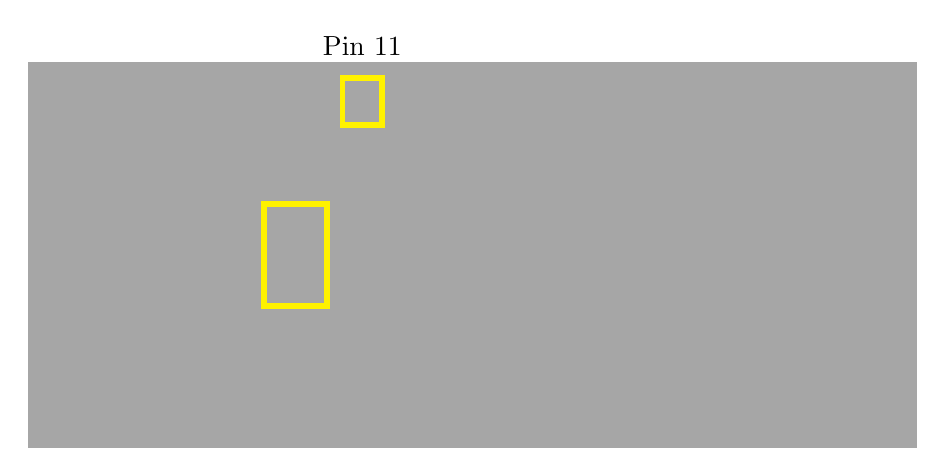
\begin{tikzpicture}
        %\node at (0,0) (Board) {\includegraphics{Arduino/Nano33BLE/Nano33BLESense}};
        
        \ArduinoNanoTikz;
        
        \fill[gray, opacity=0.7] (-11.2,-0.2) rectangle (0.1,4.7);
        
        \coordinate (A) at (-8.2,1.6);
        \coordinate (B) at (-7.4,2.9); 
        
        
        \coordinate (C) at (-7.2,3.9);
        \coordinate (D) at (-6.7,4.5);  
        
        \def\cliparea{(C) rectangle (D); (A) rectangle (B); }  
        
        \begin{scope}
            \clip (A) rectangle (B);
            
            \ArduinoNanoTikz
            
            %\node at (0,0) (Board) {\includegraphics{Arduino/Nano33BLE/Nano33BLESense}};
            
        \end{scope}
        
        %        \fill[ArduinoColor] (C) rectangle (D);
        %         \fill[gray!30] ({-8.16-0.195},4.145) rectangle ++(0.39, 0.39); 
        %        \draw[fill=gray!30,gray!30] (-8.145,4.143) circle(0.195); 
        %        \draw[fill=gray!60,gray!60] (-8.145,4.143) circle(0.165); 
        %        \fill[white,white](-8.145,{4.143+0.39}) circle (0.1275);
        
        \draw[yellow,line width=2pt] (A)  rectangle (B);
        \draw[yellow,line width=2pt] (C)  rectangle (D);
        
        \node (P25) at (-6.95, 4.9) {Pin 11};
    \end{tikzpicture}    
    
    
    
    \captionof{figure}{Arduino Nano 33 BLE Sense's built-in Push Button  with Pin 11}  
\end{center}

}






\section{Specification}

The built-in button is a small white button  and connected to pin 11.\index{Pin!Pin 11}

\begin{description}
    \item [Built-in Button:] \PYTHON{BUTTON\_B =  11u}
\end{description}

If the pin is declared as input in the function \PYTHON{setup}, then it can be used.

%\Mynote{cite data sheet, power consumption?}

The pin 11 must be defined as an input in the function \PYTHON{setup} by setting \PYTHON{pinMode (11, INPUT\_PULLUP)}, otherwise the button cannot be read.

\medskip 


The pin 11 can also be used otherwise. Then the button is not in use. \cite{Arduino:2023a,Arduino:2023,ArduinoNano33Manual:2022}

%\Mynote{What happen if there is another button at the pin? Both in use?}

\Mynote
{
\begin{itemize}
  \item cite data sheet
  \item Circuit Diagram
\end{itemize}
}

\section{Simple Code}


As soon as the button is connected, it can be used. It is not necessary to install a special library. Programming takes place in two steps:

\begin{enumerate}
    \item In the first step, the pin is configured in the function \PYTHON{setup}:
    
    {
        \captionof{code}{Defining the built-in button's pin as an input.}
        \begin{Arduino}
            pinMode(BUTTON_B, INPUT_PULLUP)   
        \end{Arduino}
    }
    \item In the second step, the button can be used in the function \PYTHON{loop}. To read in the value, use the function \PYTHON{digitalRead}:
    
    {
        \captionof{code}{Read the built-in button's state}
        \begin{Arduino}
            buttonState = digitalRead(BUTTON_B);
        \end{Arduino}
    }
    
\end{enumerate}




\section{Tests}


The simplest test is the flashing of an LED for 2 seconds, if the button is pressed, see sketch \ref{Nano:BuiltinButtonTest}.

{
    \captionof{code}{Simple sketch to test the push button and the built-in LED}\label{Nano:BuiltinButtonTest}
    \ArduinoExternal{}{../../Code/Nano33BLESense/PushButton/TestPushButton/TestPushButton.ino}
}

\section{Interrupt Function on the Arduino Nano 33 BLE Sense}


An interrupt is a function that allows the microcontroller on the Arduino Nano 33 BLE Sense to immediately respond to an external event, such as pressing a button, without the need for the program to continuously check for that event. Normally, in a program, the microcontroller would repeatedly check if a button is pressed by running through a loop, which consumes processing power and can slow down other tasks. This is not efficient, especially when the program needs to perform other actions at the same time.

With an interrupt, the program can continue running other tasks, and only when the specified event (like a button press) occurs, the program is temporarily paused to execute a special function known as the \menu{Interrupt Service Routine (ISR)}. The ISR is a small, efficient function designed to handle the event, such as changing a variable or triggering another action. After the ISR is executed, the program returns to where it left off, continuing its normal operation.

Using interrupts in this way helps make the program more efficient and responsive, as it doesn't waste time constantly checking for events and can focus on other tasks until something important happens. This is especially useful for real-time applications where quick responses to external events are necessary, such as in embedded systems, robotics, or sensor monitoring.



\section{Simple Application}



This code sketch \ref{Nano:TestButtonInterrupt} shows how to use an interrupt to control the built-in LED on the Arduino Nano 33 BLE Sense when the built-in push button is pressed.

The program sets up the built-in LED and push button. When the button is pressed, an interrupt runs a special function called an Interrupt Service Routine. The ISR is very short and only sets a flag variable \PYTHON{pushPressed} to \PYTHON{true}, indicating that the button has been pressed.

The main program \PYTHON{loop} checks this flag. If it is set to \PYTHON{true}, the program turns on the LED for 2 seconds, then turns it off and resets the flag to \PYTHON{false}. This ensures the system is ready to detect the next button press. Using the \PYTHON{true and false} values makes it easy to manage the button's state.

This method avoids constantly checking the button’s state, making the program more efficient. Additionally, the Arduino Nano 33 BLE Sense allows all its pins to be used for interrupts. This makes it easy to attach interrupt functions to any pin, allowing quick and efficient responses to inputs like buttons or sensors. \cite{ArduinoInterrupt:2019}


\Mynote{andere Überschrift für simple Application}

\bigskip







{
    \captionof{code}[Simple sketch connects the push button with an interrupt.]{Simple sketch connects the push button with an interrupt. Here, pushing the built-in button is handled by an interrupt. Then the built-in LED switch on for 2 sec.}\label{Nano:TestButtonInterrupt}
    \ArduinoExternal{}{../../Code/Nano33BLESense/PushButton/TestPushButtonInterrupt/TestPushButtonInterrupt.ino}
}

\bigskip

This is just a simple example. The variable \PYTHON{BUTTON\_B} is already defined, so the assignment is not necessary. The command \PYTHON{delay} should be avoided in an Arduino sketch. Instead, variables of the type \PYTHON{elapsedMillis} should be used.



\section{Further Readings}

\begin{itemize}
  \item Boxall, John: \textsl{Arduino Workshop - A Hands-On Introduction with 65 Projects}. No Starch Press, 2021. \cite{Boxall:2021}
  \item Vo{\"s}, Andreas: \textsl{Volumio mit Drehgebern erweitern}. Make Magazin, 2024. \cite{Voss:2024}
  \item K\"uhnel, Claus: \textsl{Arduino - Das umfassende Handbuch}. Rheinwerk Verlag GmbH, 2024. \cite{Kuehnel:2024}
\end{itemize}



  %%%%%%%%%%%%
%
% $Autor: Wings $
% $Datum: 2019-03-05 08:03:15Z $
% $Pfad: TemplateSensor $
% $Version: 4250 $
% !TeX spellcheck = en_GB/de_DE
% !TeX encoding = utf8
% !TeX root = filename 
% !TeX TXS-program:bibliography = txs:///biber
%
%%%%%%%%%%%%

% Structure
\chapter{Pressure and Temperature Sensor LPS22HB}

The sensor LPS22HB is a piezoresistive absolute pressure sensor that is integrated into the Arduino Nano 33 BLE Sense board. It's a digital sensor that measures atmospheric pressure and temperature. The sensor uses a piezoresistive technology to detect changes in pressure. The LPS22HB has an accuracy of $\pm1.5$ hPa and a resolution of 0.01 hPa. It can measure pressures from 260 to 1260 hPa. The sensor also measures temperature with an accuracy of $\pm0.12^\circ$C and a resolution of $0.01^\circ$C. The temperature range is from $-40^\circ$C to $85^\circ$C. 

The LPS22HB communicates with the Arduino board using the protocol I\textsuperscript{2}C. It has a low power consumption of 1.5 $\mu A$ in sleep mode and 1.5 mA in active mode. The sensor is also resistant to shock and vibration. It's a sensor for projects that require accurate pressure and temperature measurements, such as weather stations, altimeters. \cite{Arduino:2023a,Arduino:2023}

Arduino Nano 33 BLE Sense Lite hat  keine HTS221-Temperatur- und Feuchtigkeitssensoren, sondern nur den LPS22HB-Drucksensor, der allerdings auch die Temperatur messen kann

Arduino Nano 33 BLE Sense Rev2 hat  einen HTS221-Temperatur- und Feuchtigkeitssensor und den LPS22HB-Drucksensor, der allerdings auch die Temperatur messen kann.


Unterschiede:

Inertiale Messeinheit (IMU):
Rev 1: Verfügt über eine einzelne 9-Achsen-IMU.
Rev 2: Hat eine Kombination aus zwei IMUs: eine 6-Achsen-IMU (BMI270) und eine 3-Achsen-IMU (BMM150), was die Möglichkeiten zur Bewegungserkennung erweitert1.

Design und Zugänglichkeit:
Rev 2: Integriert neue Pads und Testpunkte für USB, SWDIO und SWCLK, was den Zugang zu diesen wichtigen Punkten auf der Platine erleichtert1.
Rev 1: Hat diese zusätzlichen Pads und Testpunkte nicht.
Stromversorgung:

Rev 2: Verwendet den MP2322 als Stromversorgungskomponente, was die Leistung verbessert1.

Rev 1: Nutzt eine andere Stromversorgungskomponente.
Der Arduino Nano 33 BLE Sense Rev 1 verwendet den MPS MP2144 als Stromversorgungskomponente

\begin{center}    
    
\begin{tikzpicture}
        %\node at (0,0) (Board) {\includegraphics{Arduino/Nano33BLE/Nano33BLESense}};
        
        \ArduinoNanoTikz;
        
        \fill[gray, opacity=0.7] (-11.2,-0.2) rectangle (0.1,4.7);
        
        \coordinate (A) at (-6.55,2.4);
        \coordinate (B) at (-5.9,3.05);    
        
        
        
        \begin{scope}
            \clip (A) rectangle (B);
            
            \ArduinoNanoTikz
            
            %\node at (0,0) (Board) {\includegraphics{Arduino/Nano33BLE/Nano33BLESense}};
            
        \end{scope}
        
        
        \draw[yellow,line width=2pt] (A)  rectangle (B);        
    \end{tikzpicture}    
    
    \captionof{figure}{Arduino Nano 33 BLE Sense's pressure and temperature sensor LPS22HB}  
\end{center}




\section{General}

A pressure sensor is a device that measures the pressure of its surroundings. It works by converting the mechanical energy of the environment into an electrical signal. The sensor typically consists of a diaphragm or membrane, which is a thin, flexible material that changes its shape in response to changes in pressure. The diaphragm or membrane is usually connected to a microcontroller or other electronic device, which reads the electrical signal and converts it into a pressure reading. The pressure sensor can be calibrated to provide accurate readings over a specific pressure range. The sensor can be used in a variety of applications, including industrial control systems, medical devices, and consumer electronics.

Pressure sensors can be classified into two main types: absolute and differential. Absolute pressure sensors measure the absolute pressure of the environment, while differential pressure sensors measure the difference in pressure between two points. Pressure sensors can be used to measure a wide range of pressures, from very low pressures to very high pressures. The accuracy of a pressure sensor depends on its calibration and the quality of its components. Pressure sensors can be affected by various factors, including temperature, humidity, and air flow. Pressure sensors can be used to monitor and control pressure in a variety of applications, including heating and cooling systems, refrigeration systems, and food processing systems. Pressure sensors can be used to detect pressure anomalies and alert users to potential problems. \cite{Gan:2024}

\bigskip

% temperatur
A temperature sensor is a device that measures the temperature of its surroundings. It works by converting the thermal energy of the environment into an electrical signal. The sensor typically consists of a thermistor or thermocouple, which is a device that changes its electrical resistance or voltage in response to changes in temperature. The thermistor or thermocouple is usually connected to a microcontroller or other electronic device, which reads the electrical signal and converts it into a temperature reading. The temperature sensor can be calibrated to provide accurate readings over a specific temperature range. The sensor can be used in a variety of applications, including industrial control systems, medical devices, and consumer electronics.

Temperature sensors can be classified into two main types: contact and non-contact. Contact temperature sensors, such as thermocouples, come into direct contact with the object being measured. Non-contact temperature sensors, such as infrared sensors, do not come into contact with the object being measured.

Temperature sensors can be used to measure a wide range of temperatures, from very low temperatures to very high temperatures. The accuracy of a temperature sensor depends on its calibration and the quality of its components. Temperature sensors can be affected by various factors, including humidity, air flow, and radiation. Temperature sensors can be used to monitor and control temperature in a variety of applications, including heating and cooling systems, refrigeration systems, and food processing systems. Temperature sensors can be used to detect temperature anomalies and alert users to potential problems.



\Mynote{cite books, applications, board}

\section{Specific Sensor}

The pressure sensor of the LPS22HB is a piezoresistive sensor that changes its electrical resistance in response to changes in pressure. The pressure sensor of the LPS22HB is connected to the Arduino Nano 33 BLE Sense, which reads the electrical signal and converts it into a pressure reading. The pressure sensor of the LPS22HB is calibrated to provide accurate readings over a pressure range of 260 to 1260 mbar. The pressure sensor of the LPS22HB is a non-contact sensor, meaning that it does not come into direct contact with the object being measured. The pressure sensor of the LPS22HB is affected by various factors, including temperature and humidity. The pressure sensor of the LPS22HB can be used to monitor and control pressure in a variety of applications, including industrial control systems and consumer electronics. The pressure sensor of the LPS22HB can be used to detect pressure anomalies and alert users to potential problems. The pressure sensor of the LPS22HB has an accuracy of $\pm0.12$ mbar. 

The pressure sensor of the LPS22HB is a low-power sensor, making it suitable for use in battery-powered devices. 

\bigskip
% Temperatur

The LPS22HB is a digital pressure sensor that also includes a temperature sensor. The temperature sensor of the LPS22HB is a thermistor that changes its electrical resistance in response to changes in temperature. The thermistor is connected to the  microcontroller Arduino Nano 33 BLE Sense, which reads the electrical signal and converts it into a temperature reading. The temperature sensor of the LPS22HB is calibrated to provide accurate readings over a temperature range of $-40^\circ$C to $85^\circ$C. The temperature sensor of the LPS22HB is a non-contact sensor, meaning that it does not come into direct contact with the object being measured. 

The temperature sensor of the LPS22HB is affected by various factors, including humidity and air flow. The temperature sensor of the LPS22HB can be used to monitor and control temperature in a variety of applications, including industrial control systems and consumer electronics. The temperature sensor of the LPS22HB can be used to detect temperature anomalies and alert users to potential problems. The temperature sensor of the LPS22HB is a high-accuracy sensor, with an accuracy of $\pm0.12^\circ$C and a resolution of $0.01^\circ$C. 

The temperature sensor of the LPS22HB is a low-power sensor, making it suitable for use in battery-powered devices. 

\Mynote{cite board}

\section{Specification}

The LPS22HB is a digital pressure sensor that measures pressure in the range of 260 to 1260 mbar. It has a high accuracy of $\pm0.12$ mbar and a resolution of 0.01 mbar. The sensor is calibrated to provide accurate readings over a temperature range of $-40^\circ$C to $85^\circ$C. It has a non-contact measurement principle, which means that it does not come into direct contact with the object being measured. The LPS22HB is a compact sensor, measuring $3.5 \times 3.5 \times 1.1$ mm in size. 

It has a low power consumption of $1.5 \mu A$ in active mode and $0.1 \mu A$ in sleep mode.

The sensor has a sampling rate of up to 100 Hz and a data transfer rate of up to 400 kbps. Note that the sampling rate of the sensor LPS22HB can be adjusted using the function \PYTHON{setSamplingRate()} in the Arduino library. The default sampling rate is 100 Hz, but it can be set to 50 Hz, 25 Hz, or 10 Hz using the following code:

\medskip

\PYTHON{lps22hb.setSamplingRate(50); // 50 Hz}

\PYTHON{lps22hb.setSamplingRate(25); // 25 Hz}

\PYTHON{lps22hb.setSamplingRate(10); // 10 Hz}

\medskip


It's worth noting that the sampling rate of the sensor LPS22HB can affect the accuracy and reliability of the measurements. A higher sampling rate can provide more accurate measurements, but it can also increase the power consumption of the sensor.


 The sensor is also resistant to shock, vibration, and temperature changes. It has a high sensitivity and a low noise level, making it suitable for use in applications where high accuracy is required. 



\begin{itemize}
  \item cite data sheet
  \item Circuit Diagram
\end{itemize}

\section{Library}

To program the sensor LPS22HB on the Arduino Nano 33 BLE Sense, you will need to use the library LPS22HB. \cite{ArduinoLPS22HB:2024}

\subsection{Description}

The library LPS22HB is a library for the Arduino platform that provides a simple interface for interacting with the sensor LPS22HB. It allows you to read temperature and pressure values from the sensor, as well as set the sensor's mode and power mode. \cite{ArduinoLPS22HB:2024}


\subsection{Installation}

To use the library LPS22HB, you will need to install it on your Arduino IDE. You can do this by following these steps:

\begin{itemize}
    \item Open the Arduino IDE and navigate to the menu \menu{Sketch}.
    \item Select \menu{Sketch -> Include Library -> Manage Libraries}.
    \item Search for ``LPS22HB'' in the library search bar.
    \item Click on the library ``LPS22HB''  and then click on the buttion ``Install''.
    \item Wait for the library to install and then restart the Arduino IDE.
\end{itemize}

\medskip

Once you have installed the library LPS22HB, you can use it to program the sensor LPS22HB on the Arduino Nano 33 BLE Sense. Here is an example~\ref{LPS22HBSimpleExample} of how you can use the library to read temperature and pressure values from the sensor:

\medskip

{
    \captionof{code}{Example code for the sensor LPS22HB on the Arduino Nano 33 BLE Sense}\label{LPS22HBSimpleExample.ino}
    \ArduinoExternal{}{../../Code/Nano33BLESense/SensorLPS22HB/LPS22HBSimpleExample.ino}
}

\medskip

This sketch \ref{LPS22HBSimpleExample.ino} uses the library LPS22HB to read temperature and pressure values from the sensor LPS22HB and print them to the serial console.

Note that you will need to have the Arduino Nano 33 BLE Sense board connected to your computer and the Arduino IDE installed on your computer in order to use the LPS22HB library.


\subsection{Functions}
Here are the functions of the Arduino library LPS22HB:

\begin{itemize}
  \item Initialization Functions
    \begin{itemize}
      \item \PYTHON{begin()}: Initializes the sensor LPS22HB and sets it up for use.
      \item \PYTHON{reset()}: Resets the sensor LPS22HB to its default state.
    \end{itemize}
  \item Reading Functions
    \begin{itemize}
      \item \PYTHON{readTemperature()}: Reads the temperature value from the sensor LPS22HB.
      \item \PYTHON{readPressure()}: Reads the pressure value from the sensor LPS22HB.
      \item \PYTHON{readAltitude()}: Reads the altitude value from the sensor LPS22HB.
      \item \PYTHON{readTemperatureAndPressure()}: Reads both the temperature and pressure values from the sensor LPS22HB.
    \end{itemize}
  \item Setting Functions
    \begin{itemize}
      \item \PYTHON{setMode()}: Sets the mode of the sensor LPS22HB.
      \item \PYTHON{setPowerMode()}: Sets the power mode of the sensor LPS22HB.
      \item \PYTHON{setSamplingRate()}: Sets the sampling rate of the sensor LPS22HB.
      \item \PYTHON{setFilter()}: Sets the filter of the sensor LPS22HB.
    \end{itemize}
  \item Getting Functions
    \begin{itemize}
      \item \PYTHON{getMode()}: Gets the current mode of the sensor LPS22HB.
      \item \PYTHON{getPowerMode()}: Gets the current power mode of the sensor LPS22HB.
      \item \PYTHON{getSamplingRate()}: Gets the current sampling rate of the sensor LPS22HB.
      \item \PYTHON{getFilter()}: Gets the current filter of the sensor LPS22HB.
    \end{itemize}
  \item Sleep Functions
    \begin{itemize}
      \item \PYTHON{sleep()}: Puts the sensor LPS22HB into sleep mode.
      \item \PYTHON{wakeUp()}: Wakes up the sensor LPS22HB from sleep mode.
    \end{itemize}
  \item Other Functions
    \begin{itemize}
      \item \PYTHON{checkStatus()}: Checks the status of the sensor LPS22HB.
      \item \PYTHON{getError()}: Gets the error code of the sensor LPS22HB.
      \item \PYTHON{resetError()}: Resets the error code of the sensor LPS22HB.
    \end{itemize}
\end{itemize}

\medskip

Note that this list may not be exhaustive, and the library may have additional functions not listed here.

\subsection{Example - Manual}

\subsection{Example}

\subsection{Example - Code}

\subsection{Example - Files}



\section{Calibration}

To calibrate the sensor LPS22HB on the Arduino Nano 33 BLE Sense, you will need to follow these steps. First, upload the calibration code to the Arduino Nano 33 BLE Sense. The calibration code will prompt you to enter the calibration parameters, such as the temperature and pressure values. Enter the calibration parameters, and the code will store them in the sensor's memory. The calibration process will take a few minutes to complete. During the calibration process, the sensor will take multiple readings of the temperature and pressure values. The sensor will then calculate the average of the readings and store it as the calibration value. Once the calibration process is complete, the sensor will be ready to use. To verify the calibration, you can use the calibration code to read the temperature and pressure values from the sensor. Compare the readings with the expected values to ensure that the sensor is calibrated correctly. If the readings are not accurate, you may need to repeat the calibration process. The calibration process can be repeated as many times as necessary to achieve accurate readings. The calibration values can be stored in the sensor's memory and retrieved later. By following these steps, you can calibrate the sensor LPS22HB on the Arduino Nano 33 BLE Sense and ensure accurate readings.

\Mynote{cite method, more mathematics!}




The code \ref{LPS22HBCalibration.ino} reads the temperature and pressure values from the sensor LPS22HB, stores them in the sensor's memory, and prints them to the serial console. The storeCalibration function is used to store the calibration values in the sensor's memory.

\medskip

{
    \captionof{code}{Simple sketch calibrating the sensor LPS22HB}\label{LPS22HBCalibration.ino}
    \ArduinoExternal{}{../../Code/Nano33BLESense/SensorLPS22HB/LPS22HBCalibration.ino}
}

\medskip


Note that this is just an example code and you may need to modify it to suit your specific needs. Additionally, you will need to make sure that the sensor LPS22HB is properly connected to the Arduino Nano 33 BLE Sense and that the I2C interface is enabled.

\section{Simple Code}

\section{Sleep Mode}



{
    \captionof{code}{Sketch for the Arduino Nano 33 BLE Sense to switch the sensor LPS22HB into sleep mode}\label{LPS22HBSleep.ino}
    \ArduinoExternal{}{../../Code/Nano33BLESense/SensorLPS22HB/LPS22HBSleep.ino}
}

\medskip


This sketch \ref{LPS22HBSleep.ino} uses the function \PYTHON{sleep()} to switch the sensor into sleep mode, and the function \PYTHON{wakeUp()} to switch the sensor out of sleep mode. The function \PYTHON{sleep()} puts the sensor into a low-power state, and the function \PYTHON{wakeUp()} restores the sensor to its normal operating state.

Note that the function \PYTHON{sleep()} must be called before the sensor can be put into sleep mode, and the function \PYTHON{wakeUp()} must be called before the sensor can be restored to its normal operating state.

Also, note that the function \PYTHON{sleep()}  can only be called when the sensor is in a valid state, and the function \PYTHON{wakeUp()} can only be called when the sensor is in a valid state.

You can also use the function \PYTHON{setMode()} to set the sensor to sleep mode, and the function \PYTHON{getMode()} to get the current mode of the sensor.

\medskip

\PYTHON{lps22hb.setMode(LPS22HB\_MODE\_SLEEP);}

\PYTHON{lps22hb.getMode();}

\medskip

This will set the sensor to sleep mode and get the current mode of the sensor.

You can also use the function \PYTHON{setPowerMode()}  to set the power mode of the sensor, and the function \PYTHON{getPowerMode()} to get the current power mode of the sensor.

\medskip

\PYTHON{lps22hb.setPowerMode(LPS22HB\_POWER\_MODE\_SLEEP);}

\PYTHON{lps22hb.getPowerMode();}


This will set the power mode of the sensor to sleep mode and get the current power mode of the sensor.

\section{Simple Application}



\section{Tests}

\subsection{Simple Function Test}

\subsection{Test all Functions}

\section{Simple Application}


\section{Further Readings}



 % %%%%%%%%%%%%%%%
%
% $Autor: Wings $
% $Datum: 2020-01-29 07:55:27Z $
% $Pfad: General/SensorAPDS9960.tex
% $Version: 1785 $
%
%
%%%%%%%%%%%%%%%

\chapter{Sensormodul APDS-9960 for Gesture, Proximity, and Color Detection}

The APDS-9960 sensor, integrated on the Arduino Nano 33 BLE Sense, is a multifunctional optical sensor used for gesture recognition, ambient light detection, color sensing, and proximity measurement. The sensor uses an I²C interface for communication and comes equipped with an additional infrared LED.
\cite{Avago:2015}


\begin{center}    
	\begin{tikzpicture}
		\node at (0,0) (Board) {\includegraphics{Arduino/Nano33BLE/Nano33BLESense}};
		
		\fill[gray, opacity=0.7] (-6,-2.4) rectangle (6,2.4);
		
		\coordinate (A) at (-1,0.4);
		\coordinate (B) at (0.2,-0.2);    
		\begin{scope}
			\clip (A) rectangle (B);
			\node at (0,0) (Board) {\includegraphics{Arduino/Nano33BLE/Nano33BLESense}};
		\end{scope}
		\draw[yellow,line width=2pt] (A) rectangle (B);
	\end{tikzpicture}    
	
	\captionof{figure}{Arduino Nano 33 BLE Sense's APDS-9960}
	\label{fig:5.1}
\end{center}

\bigskip


\Mynote{Figure 6.1 must be converted into a TikZ image to maintain consistency}

The sensor is located centrally on the Arduino Nano 33 BLE Sense, as indicated in the Figure \ref{fig:5.1}.










\section{Functionality of the APDS-9960}


The APDS-9960 is a versatile optical sensor that offers multiple functionalities, including color detection, proximity sensing, ambient light measurement, and gesture recognition. Each of these features plays a crucial role in various applications, ranging from smart lighting adjustments to touchless control systems.

In the following sections, each function of the APDS-9960 will be explored in detail, explaining its working principle, the type of data it provides, and its potential use cases.





\section{Key Technical Specifications}
\label{chap:Specification}

\subsection*{Power Supply}
\begin{itemize}
	\item Supply Voltage: 2.4 V to 3.6 V
	\item Maximum Voltage: 3.8 V
\end{itemize}

\subsection*{Power Consumption}
\begin{itemize}
	\item Active ALS Mode (Ambient Light Sensor): 200-250 µA
	\item Proximity and Gesture Modes: 790 µA (without LED)
	\item Sleep Mode: 1-10 µA
\end{itemize}

\subsection*{Temperature}
\begin{itemize}
	\item Operating Temperature Range: -30°C to +85°C
	\item Storage Temperature Range: -40°C to +85°C
\end{itemize}

\subsection*{Optical Properties}
\begin{itemize}
	\item LED Wavelength (max.): 950 nm
	\item LED Drive Current:
	\begin{itemize}
		\item 100 mA (Standard), 50 mA, 25 mA, 12.5 mA
		\item LED Boost Option: 100\%, 150\%, 200\%, 300\% (adjustable current boost)
	\end{itemize}
	\item Max Detection Distance for Color, Proximity and Gesture Sensor 0mm to 100mm
\end{itemize}

\subsection*{Proximity Sensor}
\begin{itemize}
	\item Pulse Width for Proximity Measurement: 4 µs to 32 µs
\end{itemize}

\subsection*{Gesture Sensor}
\begin{itemize}
	\item LED Pulse Count: 1 to 64 pulses
\end{itemize}

\subsection*{Connections}
\begin{itemize}
	\item I²C Communication:
	\begin{itemize}
		\item Data Rates: Up to 400 kHz
		\item Pins:
		\begin{itemize}
			\item SDA (I²C Data)
			\item SCL (I2C Clock)
			\item INT (Interrupt, Open Drain, Active Low)
			\item LDR (LED Driver Input)
		\end{itemize}
	\end{itemize}
\end{itemize}

\subsection*{Dimensions}
\begin{itemize}
	\item Length: 3.94mm
	\item Width: 2.36mm
	\item Height: 1.35mm
\end{itemize}

\cite{Avago:2015}


\section{Library \PYTHON{Arduino\_APDS9960}}

In the case of the APDS-9960 sensor, Arduino provides a library \FILE{Arduino\_APDS9960} for calling functions related to color detection, distance measurement, or gesture recognition.

The library for the sensor is \FILE{Arduino\_APDS9960}. This allows measuring gestures, colors, light intensity, and distances with the sensor. Communication between the Arduino Nano 33 BLE Sense's chip and the APDS-9960 module occurs via an internal I²C interface \cite{Avago:2015}.

The library is included by using the command \PYTHON{\#include <Arduino\_APDS9960.h>}.






\subsection{Installation of APDS-9960 Library}

The library is installed as follows:



\begin{enumerate}
	\item Open the Arduino IDE and navigate to \menu[,]{Tools,Manage Libraries...}.
	\item In the Library Manager, use the search bar to look for "Arduino\_APDS9960".
	\item Several libraries will be displayed. Select the library titled "Arduino\_APDS9960" by Arduino and click \textit{Install}.
	\item Once installed, the IDE will show a message in the console confirming the installation. The "Install" button will also change to "Remove", as seen in Figure \ref{fig:APDS9960}, indicating the library is ready for use.
\end{enumerate}


\begin{center}
	\includegraphics[width=8cm]{Arduino/APDS9960/APDS9960Installed.png}
	\captionof{figure}{APDS-9960 Library Instalation}\label{fig:APDS9960}		
\end{center} 










\subsection{Functions}

After the theoretical overview of the APDS-9960 sensor's functions, the following section will explain the practical implementations. It will demonstrate how the various functions of the sensor, such as color detection, gesture recognition, and proximity sensing, can be applied in practice to activate and evaluate the sensor's capabilities.

\medskip

Here are the codes to utilize the various functions of the APDS-9960 sensor, such as color detection, gesture recognition, and proximity sensing, see \cite{ArduinoAPDS9960:2024}:

\begin{itemize}
	\item \PYTHON{begin()}: The \PYTHON{begin()} method activates and initializes the APDS9960 sensor. It is typically called during the \PYTHON{setup\{\}} phase.
	
	\medskip
	
	\begin{itemize}
		\item Return value \PYTHON{TRUE}: Initialization was successful.
		\item Return value \PYTHON{FALSE}: Initialization failed.
	\end{itemize}
	
	\item \PYTHON{end()}: The \PYTHON{end()} method deactivates the APDS9960 sensor.
	
	
	\item \PYTHON{colorAvailable()}: This method checks if color data is available to be retrieved.
	
	\medskip
	
	\begin{itemize}
		\item Return value \PYTHON{TRUE}: Color data is available.
		\item Return value \PYTHON{FALSE}: No color data is available.
	\end{itemize}
	
	\item \PYTHON{readColor(...)}: This method retrieves the color values from the sensor.
	
	It can either read just the color values or the color values along with the ambient light intensity.
	
	\medskip
	
	To read only the color values:
	
	\PYTHON{int r, g, b;}
	
	\PYTHON{APDS.readColor(r, g, b);}
	
	\medskip
	
	The variables \PYTHON{r}, \PYTHON{g}, and \PYTHON{b} will contain the updated color values. The value range is $0, 1, 2, \ldots, 255$.
	
	\medskip
	
	To read both the color values and ambient light intensity:
	
	\PYTHON{int r, g, b, a;} 
	
	\PYTHON{APDS.readColor(r, g, b, a);}
	
	\medskip
	
	The variables \PYTHON{r}, \PYTHON{g}, and \PYTHON{b} will contain the updated color values, while \PYTHON{a} will contain the ambient light intensity. The value range is $0, 1, 2, \ldots, 255$.
	
	\item \PYTHON{proximityAvailable()}: This method checks if proximity data is available.
	
	\medskip
	
	\begin{itemize}
		\item Return value \PYTHON{TRUE}: Proximity data is available.
		\item Return value \PYTHON{FALSE}: No proximity data is available.
	\end{itemize}
	
	\item \PYTHON{readProximity()}: This method reads the proximity value.
	
	\medskip
	
	\begin{itemize}
		\item Return value \PYTHON{int proximity = APDS.readProximity()}: Returns the proximity value.
		\item Return value \PYTHON{-1}: Proximity could not be determined.
	\end{itemize}
	
	\item \PYTHON{gestureAvailable()}: This method checks if a gesture has been detected.
	
	\medskip
	
	\begin{itemize}
		\item Return value \PYTHON{TRUE}: A gesture has been detected.
		\item Return value \PYTHON{FALSE}: No gesture detected.
	\end{itemize}
	
	\item \PYTHON{setGestureSensitivity()}: Gesture detection is influenced by lighting conditions, speed, and distance of movement. This function allows you to adjust the sensitivity of gesture recognition. A higher value detects more gestures, but increases the chance of false positives. A lower value reduces the likelihood of detecting gestures.
	
	The valid range is \PYTHON{1} to \PYTHON{100}.
	
	The default value is \PYTHON{80}.
	
	\item \PYTHON{readGesture()}: If a gesture has been detected, it can be retrieved using the \PYTHON{readGesture()} method. The possible return values are:
	
	\begin{itemize}
		\item \PYTHON{GESTURE\_UP}: An upward movement has been detected.
		\item \PYTHON{GESTURE\_DOWN}: A downward movement has been detected.
		\item \PYTHON{GESTURE\_LEFT}: A leftward movement has been detected.
		\item \PYTHON{GESTURE\_RIGHT}: A rightward movement has been detected.
		\item \PYTHON{GESTURE\_NONE}: No gesture has been detected.
	\end{itemize}
	
	\item \PYTHON{setInterruptPin()}: This method sets the pin used to trigger a measurement. The pin is usually detected automatically, but can be set manually using this function.
	
	If \PYTHON{-1} is passed, no pin is connected.
	
	If \PYTHON{0} or a higher value is passed, that pin will be used.
	
	The default value depends on the board.
	
	\item \PYTHON{setLEDBoost(...)}: The sensor includes an infrared LED that can be temporarily boosted to provide higher brightness. It can be set to provide up to 300\% of its normal power. This can be configured using this method.
	
	\medskip
	
	Usage:
	
	\begin{itemize}
		\item \PYTHON{0}: Boost to 100\% (default power).
		\item \PYTHON{1}: Boost to 150\%.
		\item \PYTHON{2}: Boost to 200\%.
		\item \PYTHON{3}: Boost to 300\%.
	\end{itemize}    
	
	\medskip
	
	Return values:
	
	\begin{itemize}
		\item \PYTHON{0}: Failure.
		\item \PYTHON{1}: Success.
	\end{itemize}
\end{itemize}




\section{Simple Function Tests}

The following code examples can be used to test and try out all functions of the APDS-9960.

\subsection{Example Color Detection}

The library  \PYTHON{Arduino\_APDS9960} includes an example code demonstrating how to perform color detection with the sensor APDS-9960 on an Arduino Nano 33 BLE Sense. This example also tests the ambient light sensor, as both functionalities rely on the same underlying technology. The measured color channel intensities (Red, Green, and Blue) are displayed in the Serial Monitor for real-time observation.

The sensor APDS-9960 enables accurate RGB color detection by measuring the intensity of red, green, and blue light reflected from an object. These values can be visualized in the Serial Plotter, allowing users to track changes in color intensity over time through a graphical representation. This feature is particularly useful for applications that require real-time color monitoring or dynamic light adjustments.


\subsection{Example Color Detection - Manual}

\Mynote{to do}


\subsection{Setting Up the Color Sensor Measurement Program}

To begin the process of creating the color sensor measurement program, open the Arduino Cloud Editor and navigate to the "Libraries" tab. Search for the "Arduino-APDS9960" library and download it. Afterward, click on "More info" to access the GitHub repository, where several examples are provided.

Next, connect the Arduino Nano 33 BLE Sense to the computer, ensuring that the Cloud Editor detects both the board and the corresponding port. If the board is not automatically recognized, follow the instructions to install the necessary plugin to enable the editor to detect the board. Confirm that the correct port is selected. Finally, upload the program to the Arduino, and by opening the serial monitor, the measured values will be recorded in the Arduino IDE.

\subsection{Example }Color Detection - Code}

First, serial communication is started with \PYTHON{Serial.begin(9600)} to send data to the computer. The command  \PYTHON{APDS.begin()} initializes the sensor and in the event of a potential error, an error message is output via the serial interface.

\bigskip



\bigskip

The code operates within the function \PYTHON{loop()} of a sketch to continuously read and display color values from the APDS-9960 sensor. Initially, it checks if a color reading is available by using the method \PYTHON{APDS.colorAvailable()}. If no reading is available, the program briefly pauses for 5 milliseconds to avoid excessive CPU usage. Once a reading is ready, the method \PYTHON{APDS.readColor(r, g, b)} retrieves the color data and stores the red, green, and blue values in the respective variables. These values are then printed to the Serial Monitor, labeled clearly as ``r'', ``g'', and ``b''. A one-second delay is added before the program repeats the loop, allowing for clear intervals between consecutive readings.




\subsection{Example Color Detection - File}

The program can be found at 

\medskip

{
	\captionof{code}{Simple sketch using the sensor APDS9960 for colors}\label{TestAPDS9960Color}
	\ArduinoExternal{}{../../Code/Nano33BLESense/APDS9960/TestAPDS9960Color/TestAPDS9960Color.ino}
}


\subsection{Proximity}

A simple code for testing the proximity sensor is also provided by the library. The proximity sensor is designed for measuring distances of up to 100mm.

\subsection{Proximity - Manual}

Open the Arduino Cloud Editor and navigate to the Libraries tab. In the search bar, search for the library \PYTHON{Arduino\_APDS9960}. Once located, open the Examples section within the library and select the sketch ``ProximitySensor''.
\smallskip
Connect the Arduino Nano 33 BLE Sense to the computer. Check that the Cloud Editor recognizes the board by verifying if both the board and port are listed in the dropdown menu.

\subsection{Example Proximity - Code}

First, serial communication is started with \PYTHON{Serial.begin(9600)} to send data to the computer. The method \PYTHON{APDS.begin()}  initializes the sensor and in the event of a potential error, an error message is output via the serial interface.


\bigskip


The code operates within the function \PYTHON{loop()}  of a sketch to continuously read and display proximity values from the sensor APDS-9960. It begins by checking if a proximity reading is available using the method \PYTHON{APDS.proximityAvailable()}. If a reading is ready, the method \PYTHON{APDS.readProximity()} retrieves the proximity value, where \PYTHON{0} indicates a close object, \PYTHON{255} indicates a distant object, and \PYTHON{-1} signals an error in reading. This proximity value is then printed to the Serial Monitor. A delay of 100 milliseconds is added before the program repeats the loop, ensuring a brief interval between consecutive readings.


\subsection{Example Proximity - File}

The sketch can be found at 

\bigskip

{
	\captionof{code}{Simple sketch using the sensor APDS9960 for measuring the proximity}\label{TestAPDS9960Proximity}
	\ArduinoExternal{}{../../Code/Nano33BLESense/APDS9960/TestAPDS9960Proximity/TestAPDS9960Proximity.ino}
}

\subsection{Gesture Detection}
\subsection{Example Gesture Detection}

The library \FILE{Arduino\_APDS9960} also provides an example sketch demonstrating gesture detection with the sensor APDS-9960 on an Arduino Nano 33 BLE Sense. Some LED feedback signals have been programmed to provide quick visual feedback.

\subsection{Example Gesture Detection - Manual}

\Mynote{to do}


\subsection{Example Gesture Detection - Code}

In this example sketch, the library \FILE{Arduino\_APDS9960} is integrated first and then the setup is created. In addition, the LED pins are configured so that they behave as outputs.


\bigskip

After that, serial communication is initialized, and the program verifies whether the sensor is correctly initialized using \PYTHON{APDS.begin()}. If initialization fails, an error message is printed. The gesture sensitivity can be adjusted via \PYTHON{APDS.setGestureSensitivity(value)}, where values range from 1 to 100, affecting detection accuracy and sensitivity. The sketch sets a default sensitivity and signals the start of gesture detection by turning off the RGB LEDs with \PYTHON{digitalWrite(LEDR, HIGH)}, \PYTHON{digitalWrite(LEDG, HIGH)}, and \PYTHON{digitalWrite(LEDB, HIGH)}.

In the function \PYTHON{loop()}, the code continuously checks for available gestures using \PYTHON{APDS.gestureAvailable()}. When a gesture is detected, it is read using \PYTHON{APDS.readGesture()} and interpreted within a \PYTHON{switch} statement. Each gesture corresponds to specific LED behavior:

\begin{itemize}
	\item \PYTHON{GESTURE\_UP}: The red LED is briefly turned on, then off after a 1-second delay.
	\item \PYTHON{GESTURE\_DOWN}: The green LED is briefly turned on, then off after a 1-second delay.
	\item \PYTHON{GESTURE\_LEFT}: The blue LED is briefly turned on, then off after a 1-second delay.
	\item \PYTHON{GESTURE\_RIGHT}: All LEDs are turned on simultaneously, then off after a 1-second delay.
\end{itemize}

The \PYTHON{default} case ensures no action if an undefined gesture is detected.



\subsection{Example Gesture Detection - File}

The sketch can be found at 

\bigskip

{
	\captionof{code}{Simple sketch using the sensor APDS9960 for gesture detection}\label{TestAPDS9960Gesture}
	\ArduinoExternal{}{../../Code/Nano33BLESense/APDS9960/TestAPDS9960Gesture/TestAPDS9960Gesture.ino}
}

\subsection{Troubleshoot}


Errors in color detection can be caused by insufficient lighting in the room. Please ensure that the environment is bright enough for the color detection function.


\section{Calibration Color Detection}

\section{Calibration Color Detection}

Due to variations in environmental light conditions and the sensitivity of the sensor, calibration is required to ensure accurate color detection. This section outlines the calibration process using a standard color chart under constant lighting conditions. To carry out the calibration, the Arduino, a connection cable (USB A to USB Micro), and a laptop or computer with the appropriate Arduino development environment are required.

\medskip

The proximity and gesture feature is pre-configured and factory-calibrated to detect proximity and gesture at a distance of 100mm, eliminating the need for customer calibration.
\cite{BroadcomAPDS9960:2024}

\subsection{Calibration Setup}

A standardized color chart is used, which provides reference values for perfect red, green, and blue under constant lighting conditions. The RGB values from the sensor are read as raw, uncalibrated data, which must be normalized to a standard range (0–255) for accurate color detection.\Mynote{citation, picture}

\subsection{Step 1: Measuring Reference Values}

The first step in the calibration process is to measure the raw sensor values for each primary color (red, green, and blue) using the standardized color chart. By placing the color chart in front of the sensor and reading the raw RGB values, we can establish the maximum possible sensor readings for each color channel.

\[
\text{RawRed} = \max(R_{\text{measured}})
\]
\[
\text{RawGreen} = \max(G_{\text{measured}})
\]
\[
\text{RawBlue} = \max(B_{\text{measured}})
\]

These maximum values are obtained by positioning the chart at a fixed distance of one centimeter and ensuring constant light intensity.

\subsection{Step 2: Normalizing the Sensor Values}
Once the maximum sensor readings for red, green, and blue are obtained, the raw sensor data is normalized to a 0-255 scale. This ensures that the sensor's readings correspond to standard RGB values. The following formula is used for normalization:

\[
R_{\text{calibrated}} = \frac{R_{\text{raw}}}{\text{RawRed}} \times 255
\]
\[
G_{\text{calibrated}} = \frac{G_{\text{raw}}}{\text{RawGreen}} \times 255
\]
\[
B_{\text{calibrated}} = \frac{B_{\text{raw}}}{\text{RawBlue}} \times 255
\]

Where:

\begin{itemize}
	\item $R_{\text{raw}}, G_{\text{raw}}, B_{\text{raw}}$ are the raw sensor values for each channel.
	\item $\text{RawRed}, \text{RawGreen}, \text{RawBlue}$ are the maximum measured values from the standard color chart.
\end{itemize}

\subsection{Step 3: Implementing the Calibration in Code}

The normalization process is implemented directly in the Arduino code to adjust the sensor's readings. To begin calibration, open the Serial Monitor, enter ``OK'' in the command line, and press Enter to confirm. The following steps will then be explained through text output.

\bigskip

After the user initiates the calibration by typing ``OK'' into the Serial Monitor, the sketch starts. The sketch guides the user through the calibration of red, green, and blue colors, with each phase confirmed by entering ``OK''. The pins for the RGB LEDs are defined, and variables store the maximum calibration values for each color. Status variables control the sequence, ensuring each phase is completed before moving to the next. These maximum values are later used for accurate color detection in the Application code.

\bigskip


The following code section begins by initializing serial communication at a baud rate of 9600, enabling interaction through the serial monitor. Next, it sets the RGB LED pins as outputs and turns on all LEDs to create white light, which helps capture accurate color measurements. The code then initializes the sensor APDS-9960, checking for successful setup. If the sensor fails to initialize, an error message is printed, and the program halts. If successful, a message confirms initialization and prompts the user to type ``OK'' in the serial monitor to proceed with the calibration process explanation.

\bigskip

The next code segment in the loop first checks if the user has entered ``OK'' to start the calibration process. After confirmation, it displays an explanation and instructions. After showing the explanation, it waits for the user to confirm by typing ``OK'' again, which then initiates the red color calibration by prompting the user to place the red chart in front of the sensor. The loop pauses at each step until the user confirms.

\Mynote{Screen shot?}

\bigskip

Each color calibration starts after the user types ``OK'' in the Serial Monitor. The sketch measures the highest detected value for each color over 10 seconds and sets it as the calibration maximum. After all colors are calibrated, it displays the final maximum values for red, green, and blue in the Serial Monitor, completing the process. The \PYTHON{maxRed}, \PYTHON{maxGreen}, and \PYTHON{maxBlue} values can later be entered into the application sketch to apply the calibration to the sketch.


\subsection{Calibration File}

The sketch can be found at 

\bigskip

{
	\captionof{code}{APDS-9960: Example Calibration}
	\ArduinoExternal{}{../../Code/Nano33BLESense/APDS9960/APDS9960Calibration/APDS9960Calibration.ino}
}


\subsection{Step 4: Validating the Calibration}

To ensure the calibration is successful, the sensor readings should be tested again using the standard color chart. The calibrated values for red, green, and blue should be close to 255 for the respective pure colors on the chart. If the readings deviate significantly, further adjustment of the maximum reference values may be necessary.

\bigskip

The calibration of the sensor APDS-9960 is essential for accurate RGB detection. By using a standard color chart and constant lighting conditions, the sensor's raw values can be normalized to provide consistent and reliable color readings. This process can be further refined by adjusting for specific environmental factors or sensor placement.


\section{Tests}

\subsection{Simple Function Test}

\subsection{Test all Functions}

\section{Simple Application}

Similarly, by following all the steps for uploading and compiling the sketch we can see the results of sensor APDS-9960  on Serial Monitor, too. For seeing the different output, we can change the input for the sensor too, e.g: for color detection we can switch the colors, for gesture detection we can also switch the gestures, and for proximity also do the same. The resulted output as shown in the figure.  \ref{fig:2} 

\Mynote{rewrite and extend}

\begin{center}
	\includegraphics[width=9.5cm]{Nano33BLESense/APDS-Output}
	\captionof{figure}{Gesture, Proximity, Color Sensor Output Window}
	\label{fig:2}
\end{center}

We can also run the single funcnality of this sensor too, e.g; if we just need to capture the color of product, we can also run the color detection program. It depends upon the application and we can implement our application and modify the code as per our desire results.


{
	\captionof{code}{Simple sketch using the sensor APDS9960}\label{TestAPDS9960}
	\ArduinoExternal{}{../../Code/Nano33BLESense/APDS9960/TestAPDS9960/TestAPDS9960.ino}
}




%%%%%%%%%%%%%%%%%%%%%%%%%%%%%%%%%%


\section{Further Readings}

\begin{itemize}
	%    \item S. Grzesik, R. Kluwak, and B. Plikusinski, "Multispectral Sensor Application Possibility Research for Temperature Measurement," \textit{2023 23rd International Conference on Mechatronics - Mechatronika (ME)}, Brno, Czech Republic, pp. 1-6, 2023. Available at: \url{https://ieeexplore.ieee.org/document/10349583}
	
	\item SparkFun Electronics, ``APDS-9960 RGB and Gesture Sensor Hookup Guide''. A comprehensive guide that explains the functionality of the APDS-9960 and provides step-by-step instructions for implementation. Available at: \url{https://learn.sparkfun.com/tutorials/apds-9960-rgb-and-gesture-sensor-hookup-guide/all}, \cite{Hymel:2024}
	
	\item Maker Guides, ``APDS-9960 Gesture and Color Sensor with Arduino''. This tutorial provides a hands-on introduction to using the APDS-9960 sensor with Arduino, including gesture and color recognition. Available at: \url{https://www.makerguides.com/apds-9960-gesture-and-color-sensor-with-arduino/}, \cite{Maetschke:2024}
\end{itemize}




 % %%%%%%%%%%%%
%
% $Autor: Wings $
% $Datum: 2019-03-05 08:03:15Z $
% $Pfad: TemplateSensor $
% $Version: 4250 $
% !TeX spellcheck = en_GB/de_DE
% !TeX encoding = utf8
% !TeX root = filename 
% !TeX TXS-program:bibliography = txs:///biber
%
%%%%%%%%%%%%

% Structure
\chapter{Sensor APDS 9960 Gesture}

Introduction
\Mynote{cite books, applications, board}



\subsection{Sensormodul APDS 9960 for Gesture}


\subsubsection{Function of the Gesture Detection Sensor}

The gesture recognition of the APDS-9960 is based on four additional angled photodiodes

\begin{itemize}
	
	\item Up – Hand movement upwards.
	\item Down – Hand movement downwards.
	\item Left – Hand movement to the left.
	\item Right – Hand movement to the right.
	
\end{itemize}

which detect reflected infrared light (IR) from the integrated IR-LED. By analyzing the reflection, which measures direction-dependent changes using the photodiodes, the sensor can recognize movements and gestures such as swiping motions in different directions (e.g., up, down, left, right). The sensor converts this information into digital data, such as speed, direction, and distance of the movement. The 32-record FIFO register allows the sensor to temporarily store motion data, ensuring continuous processing.
\smallskip
\cite{Avago:2015}


\section{General}

General description

cite books

\section{Specific Sensor}

cite board

\section{Specification}

\begin{itemize}
  \item cite data sheet
  \item Circuit Diagram
\end{itemize}

\section{Bibliothek}

\subsection{Description}

\subsection{Installation}

\subsection{Functions}

\subsection{Example - Manual}

\subsection{Example}

\subsection{Example - Code}

\subsection{Example - Files}



\section{Calibration}

cite method

\section{Simple Code}


\section{Simple Application}



\section{Tests}

\subsection{Simple Function Test}

\subsection{Test all Functions}

\section{Simple Application}


\section{Further Readings}


 % %%%%%%%%%%%%
%
% $Autor: Wings $
% $Datum: 2019-03-05 08:03:15Z $
% $Pfad: TemplateSensor $
% $Version: 4250 $
% !TeX spellcheck = en_GB/de_DE
% !TeX encoding = utf8
% !TeX root = filename 
% !TeX TXS-program:bibliography = txs:///biber
%
%%%%%%%%%%%%

% Structure
\chapter{Sensor APDS 9960 Color}



The general functionality of a color sensor is based on the reflection of white light from the object to be measured. White light contains wavelengths that cover the entire visible spectrum (p. 189 \cite{Rybach:2013}). Due to the molecular structure of the object or chemical processes, such as photosynthesis, certain wavelengths are absorbed while others are reflected. The reflected light rays that reach the color sensor are spectrally selected by color filters or a diffraction grating  \cite{Hering:2023}. 

\section{General}

\textbf{Color filters}: By using parallel red, green, and blue color filters, the intensities of the RGB components are evaluated by three photodiodes behind the filters \cite{Hering:2023}.

\textbf{Diffraction grating}: As light passes through a diffraction grating, the physical diffraction effect occurs. This effect, due to the varying wavelengths of light, produces an interference pattern that enables the spectral decomposition of the light. The spectrum of the incoming light is spatially dispersed, similar to the refraction in a prism (p. 208 ff. \cite{Rybach:2013}). The intensity of the color components can be measured by an array of spatially arranged photodiodes. Diffraction gratings offer higher resolution than color filters \cite{Hering:2023}.

Photodiodes are semiconductors that generate electrical energy through the internal photoelectric effect (p. 220 \cite{Rybach:2013}). The signal from the photodiodes is amplified and stored in a data register through analog-to-digital conversion. The measurement is taken over a specific period. By accumulating the RGB data, the measured color can finally be determined \cite{Avago:2015}. 

Color sensors are typically used in image processing and quality control applications \cite{Avago:2015}.



As shown in Figure \ref{fig:SchematicColorSensor}, the incoming light first passes through UV and IR filters. It is then separated into its red, green, blue, and unfiltered components by color filters. These filtered components are subsequently converted from analog to digital units, as described below.

\begin{center}
	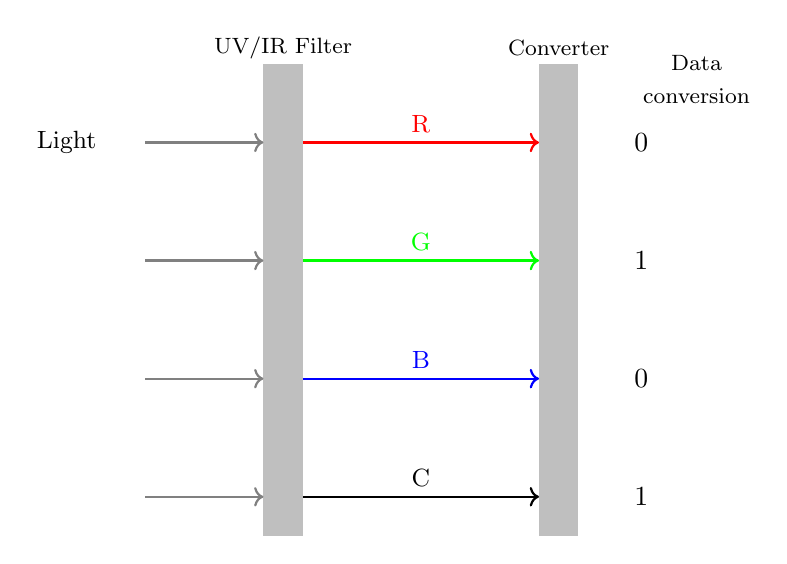
\begin{tikzpicture}
		
		% UV/IR Filter and Converter rectangles
		\fill[gray!50] (2, -2.5) rectangle (2.5, 3.5);
		\fill[gray!50] (5.5, -2.5) rectangle (6, 3.5);
		
		% Labels
		\node at (-0.5, 2.5) {\small Light};
		\node at (2.25, 3.7) {\footnotesize UV/IR Filter};
		\node at (5.75, 3.7) {\footnotesize Converter};
		\node[align=center] at (7.5, 3.3) {\footnotesize Data \\ \footnotesize conversion};
		
		% Arrows for light input
		\draw[->, thick, gray] (0.5, 2.5) -- (2, 2.5);
		\draw[->, thick, gray] (0.5, 1) -- (2, 1);
		\draw[->, thick, gray] (0.5, -0.5) -- (2, -0.5);
		\draw[->, thick, gray] (0.5, -2) -- (2, -2);
		
		% Color-coded arrows
		\draw[->, thick, red] (2.5, 2.5) -- (5.5, 2.5) node[midway, above] {\small R};
		\draw[->, thick, green] (2.5, 1) -- (5.5, 1) node[midway, above] {\small G};
		\draw[->, thick, blue] (2.5, -0.5) -- (5.5, -0.5) node[midway, above] {\small B};
		\draw[->, thick, black] (2.5, -2) -- (5.5, -2) node[midway, above] {\small C};
		
		% Data conversion outputs
		\node at (6.8, 2.5) {0};
		\node at (6.8, 1) {1};
		\node at (6.8, -0.5) {0};
		\node at (6.8, -2) {1};
	\end{tikzpicture}
	
	\captionof{figure}{Schematic of the main function of a color sensor}
	\label{fig:SchematicColorSensor}
\end{center}

The block diagram \ref{fig:FunctionalBlockDiagram} shows the processing flow of the APDS-9660 from light detection to communication via the I²C protocol with the Arduino. The individual steps are explained as follows:

\tikzstyle{block} = [rectangle, draw, minimum width=3.5cm, minimum height=1.2cm, text centered, text width=3.5cm]
\tikzstyle{smallblock} = [rectangle, draw, minimum width=3.5cm, minimum height=1.2cm, text centered]
\tikzstyle{arrow} = [thick,->,>=stealth]
\tikzstyle{sensor} = [draw, isosceles triangle, isosceles triangle apex angle=60, shape border rotate=-90, minimum height=1.5cm, minimum width=1.5cm, text centered]

\begin{center}
	\begin{tikzpicture}[node distance=2.5cm, scale=0.5, every node/.style={transform shape}]
		
		% Sensors
		\node (clear) [sensor] {Clear};
		\node (red) [sensor, below of=clear] {Red};
		\node (green) [sensor, below of=red] {Green};
		\node (blue) [sensor, below of=green] {Blue};
		
		% RGBC + ALS
		\node (rgbc_als) [block, right of=red, xshift=3cm] {RGBC \\ ALS};
		
		% MUX
		\node (mux) [smallblock, right of=rgbc_als, xshift=3cm] {MUX};
		
		% ADC
		\node (adc) [smallblock, right of=mux, xshift=3cm] {ADC};
		
		% FIFO + Threshold Control
		\node (fifo) [block, right of=adc, xshift=3.5cm] {32 x 4 Byte FIFO \\ Threshold Control};
		
		% I2C Interface
		\node (i2c) [block, above of=fifo, yshift=2cm] {I\textsuperscript{2}C Interface};
		
		% Interrupt
		\node (interrupt) [smallblock, below of=fifo, yshift=-2cm] {Interrupt};
		
		% Connections
		\draw [arrow] (clear) -- (rgbc_als);
		\draw [arrow] (red) -- (rgbc_als);
		\draw [arrow] (green) -- (rgbc_als);
		\draw [arrow] (blue) -- (rgbc_als);
		\draw [arrow] (rgbc_als) -- (mux);
		\draw [arrow] (mux) -- (adc);
		\draw [arrow] (adc) -- (fifo);
		\draw [arrow] (fifo) -- (i2c);
		\draw [arrow] (fifo) -- (interrupt);
		\draw [arrow] (i2c) -- ++(2.5cm,0) node[right] {SCL};
		\draw [arrow] (i2c) -- ++(2.5cm,-1.5cm) node[right] {SDA};
		\draw [arrow] (interrupt) -- ++(2.5cm,0) node[right] {INT};
		
	\end{tikzpicture}
	
	\captionof{figure}{Functional Block Diagram}
	\label{fig:FunctionalBlockDiagram}
\end{center}

\Mynote{The graphic is not optimal. Description of the individual blocks is not clear. What does RGBC and ALS mean?}


The photodiodes convert the intensities of the color components of the filtered light and the total light into electrical signals.
These RGBC (Red, Green, Blue, Clear) and ALS (Ambient Light Sensor) signals are forwarded to the next processing stage using the multiplexer (MUX). 

The MUX allows for the sequential processing of the color signals, as the ADC (Analog-to-Digital Converter) can only process one signal at a time.
The ADC converts the analog signal selected by the MUX into a digital value. This conversion is necessary to make the signal suitable for digital processing and transmission.

The digital value is stored in a FIFO (First In, First Out) data register, which can store up to 32 data values (4 bytes each). A threshold controller monitors the data and triggers an interrupt when defined limits are reached. The detailed process is explained in Chapter Data Processing \ref{chap:Data Processing}.

The stored data is transmitted to the Arduino via an I²C bus. The I²C bus uses two lines: the SCL (Serial Clock Line) for the clock and the SDA (Serial Data Line) for data transmission. The detailed functioning of the I²C bus is explained in Chapter \ref{chap:Protokoll I²C} Protokoll I²C.
\cite{Avago:2015}.

\subsubsection{Data Processing}
\label{chap:Data Processing}

The color detection begins at the photodiodes with RGBC detection and ends with 16-bit values stored in the RGBC data registers. The signal from the photodiode array is accumulated over a period defined by the value in the ATIME register (ALS ADC Integration Time) before the results are transferred to the RGBCDATA registers. The gain factor can be set from 1x to 64x, which is controlled via the CONTROL<AGAIN> bit (ALS Gain Control). Performance parameters such as accuracy, resolution, conversion speed, and energy consumption can be adjusted to meet the application requirements.

Between measurements, a customizable, energy-efficient waiting period is maintained, the duration of which is determined by the control bits WEN (Wait Enable), WTIME (Wait Time), and WLONG (Wait Long Enable). The waiting time can range from 0 seconds to a maximum of 8.54 seconds.

An interrupt is triggered when the clear channel values exceed the thresholds defined in the AILTL/AIHTL (ALS low threshold, lower byte/ALS high threshold, lower byte) or AILTH/AIHTH (ALS low threshold, upper byte/ALS high threshold, upper byte) threshold registers. To avoid unwanted or false interrupts, a persistence filter is integrated, ensuring that an interrupt is triggered only when a defined number of consecutive values fall outside the thresholds. This threshold is set in the APERS register (ALS Interrupt Persistence). If a value is within the thresholds, the persistence counter is reset. If the analog circuit is saturated, the ASAT bit is set, indicating potentially inaccurate RGBCDATA results. The AINT (ALS Interrupt) and CPSAT (Clear Diode Saturation) bits can be queried at any time via I²C. However, for AINT to trigger a hardware interrupt on the INT pin, the AIEN bit (ALS Interrupt Enable) must be set. Saturation of the analog-to-digital converter can be detected via the CPSAT bit; to enable this function, the CPSIEN bit (Clear Diode Saturation Interrupt Enable) must be set. The AVALID bit (ALS Valid) is reset by reading the RGBCDATA. ASAT and AINT can be reset via the CICLEAR (Clear Channel Interrupt Clear) or AICLEAR (All Non-Gesture Interrupt Clear) bits.

The RGBC results can be used to determine the color temperature in Kelvin or the ambient light intensity in Lux.

\cite{Avago:2015}








\section{Specific Sensor}

cite board

\section{Specification}

\begin{itemize}
  \item cite data sheet
  \item Circuit Diagram
\end{itemize}

\section{Bibliothek}

\subsection{Description}

\subsection{Installation}

\subsection{Functions}

\subsection{Example - Manual}

\subsection{Example}

\subsection{Example - Code}

\subsection{Example - Files}



\section{Calibration}

cite method

\section{Simple Code}


\section{Simple Application}



\section{Tests}

\subsection{Simple Function Test}

\subsection{Test all Functions}

\section{Simple Application}


\section{Further Readings}


 % %%%%%%%%%%%%
%
% $Autor: Wings $
% $Datum: 2019-03-05 08:03:15Z $
% $Pfad: TemplateSensor $
% $Version: 4250 $
% !TeX spellcheck = en_GB/de_DE
% !TeX encoding = utf8
% !TeX root = filename 
% !TeX TXS-program:bibliography = txs:///biber
%
%%%%%%%%%%%%

% Structure
\chapter{Sensor APDS 9960 Proximity}

The proximity sensor is part of the gesture detection sensor and detects top-bottom gestures based on the temporal change in the measured distance. The proximity detection measures the distance between the sensor and an object by capturing the reflected IR light. The integrated IR LED emits light, which is measured by the same photodiodes as in gesture detection. The stronger the reflection, the closer the object is. The proximity sensor can also detect events such as the approach or withdrawal of an object and trigger corresponding interrupts when predefined thresholds are exceeded. To ensure reliable measurements, the sensor compensates for unwanted reflections by adjusting offset values and suppresses interference from ambient light.
\smallskip
\cite{Avago:2015}



\section{General}

General description

cite books

\section{Specific Sensor}

cite board

\section{Specification}

\begin{itemize}
  \item cite data sheet
  \item Circuit Diagram
\end{itemize}

\section{Bibliothek}

\subsection{Description}

\subsection{Installation}

\subsection{Functions}

\subsection{Example - Manual}

\subsection{Example}

\subsection{Example - Code}

\subsection{Example - Files}



\section{Calibration}

cite method

\section{Simple Code}


\section{Simple Application}



\section{Tests}

\subsection{Simple Function Test}

\subsection{Test all Functions}

\section{Simple Application}


\section{Further Readings}


 % %%%%%%%%%%%%
%
% $Autor: Wings $
% $Datum: 2019-03-05 08:03:15Z $
% $Pfad: TemplateSensor $
% $Version: 4250 $
% !TeX spellcheck = en_GB/de_DE
% !TeX encoding = utf8
% !TeX root = filename 
% !TeX TXS-program:bibliography = txs:///biber
%
%%%%%%%%%%%%

% Structure
\chapter{Sensor Ambient Light}

The ambient light sensor (ALS) of the APDS-9960 works with the same photodiode array and measures the intensity of the ambient light. For this purpose, the UV and IR light filters are installed in front of the photodiodes to ensure accurate measurements of visible light. The sensor converts the measured light intensity into 16-bit data, which enables high resolution and accuracy. A function of programmable gain and customizable integration time ensures that the sensor can operate accurately in different lighting conditions, such as dim or very bright light.
\medskip
Another important feature of the sensor is its ability to correctly detect the intensity of ambient light even behind dark glass, which is particularly useful for devices with tinted covers.
\smallskip
\cite{Avago:2015}


\section{General}

General description

cite books

\section{Specific Sensor}

cite board

\section{Specification}

\begin{itemize}
  \item cite data sheet
  \item Circuit Diagram
\end{itemize}

\section{Bibliothek}

\subsection{Description}

\subsection{Installation}

\subsection{Functions}

\subsection{Example - Manual}

\subsection{Example}

\subsection{Example - Code}

\subsection{Example - Files}



\section{Calibration}

cite method

\section{Simple Code}


\section{Simple Application}



\section{Tests}

\subsection{Simple Function Test}

\subsection{Test all Functions}

\section{Simple Application}


\section{Further Readings}



 % \InputLanguage{Contents/General/}{AppADPS9960}

 % \InputLanguage{Contents/General/}{MicrophoneMP34DT05}

  \InputLanguage{Contents/General/}{IMU}
  \input{../../Contents/General/IMUSoftware}
  \input{../../Contents/General/IMUCalibration}
  \input{../../Contents/General/IMUErrors}
  \input{../../Contents/General/IMULibFunctions}
  %%%
%
% $Autor: Wings $
% $Date: 2024-10-31 11:15:45Z $
% $File: AccelerationDetectionAlgorithms.tex $
% $Version: 1 $
%
%%%


\chapter{Distance,  Speed and Acceleration Detection Algorithms}

\section{Review of Distance Measurement Methods}

Since Mitsubishi released the first cruise control with distance control in 1995, the vast majority of ACC functions have been based on Laser Radar or millimeter-wave radar (MWR). \footnote{MI-PILOT, Mitsubishi Motors, \url{https://www.mitsubishi-motors.com/en/brand/technology/mipilot2/index.html}} But a few have opted to use a binocular camera as the basis for the technology, such as Subaru's EyeSight technology. \footnote{EyeSight technology, Subaru, \url{https://www.subaru.com/eyesight.html}}

Each of these different sets of technical solutions has its own advantages and disadvantages:

\begin{table}[h]
	\centering
	\resizebox{\textwidth}{!}{
		\begin{tabular}{|p{3cm}|p{6cm}|p{6cm}|}
			\hline
			\textbf{Technology} & \textbf{Advantages} & \textbf{Disadvantages} \\ \hline
			\textbf{Laser Radar (LiDAR)} & 
			\begin{tabular}[c]{@{}p{6cm}@{}}
				- High accuracy and resolution \\
				- Capable of creating detailed 3D maps \\
				- Effective for object detection and classification
			\end{tabular} &
			\begin{tabular}[c]{@{}p{6cm}@{}}
				- Expensive \\
				- Affected by adverse weather conditions \\
				- High power consumption
			\end{tabular} \\ \hline
			
			\textbf{Millimeter-Wave Radar} &
			\begin{tabular}[c]{@{}p{6cm}@{}}
				- Less affected by weather conditions \\
				- Long-range detection capabilities \\
				- Lower cost compared to LiDAR
			\end{tabular} &
			\begin{tabular}[c]{@{}p{6cm}@{}}
				- Lower resolution than LiDAR \\
				- Limited in detecting small or non-metallic objects \\
				- Can be affected by interference
			\end{tabular} \\ \hline
			
			\textbf{Binocular Camera Systems} &
			\begin{tabular}[c]{@{}p{6cm}@{}}
				- Lower cost compared to LiDAR and radar \\
				- High resolution for nearby objects \\
				- Uses passive sensing (no emissions)
			\end{tabular} &
			\begin{tabular}[c]{@{}p{6cm}@{}}
				- Computationally intensive \\
				- Accuracy decreases with distance \\
				- Affected by lighting conditions
			\end{tabular} \\ \hline
		\end{tabular}
	}
	\caption{Comparison of distance measurement technologies: LiDAR, Millimeter-Wave Radar, and Binocular Cameras}
	\label{tab:comparison}
\end{table}

For cars using Laser Radar, LiDAR operates by emitting laser pulses towards objects in front of the vehicle. When these pulses hit an object, they are reflected back to the sensor, which measures the time it takes for the pulses to return. This time-of-flight measurement allows the system to calculate the precise distance to the object, as well as its relative speed and position. For cars using millimeter-wave radar, the functional implementation is similar.

For systems that use binocular cameras, this process can be relatively more complex; essentially distance recognition for binocular camera-based systems utilizes bionics: Binocular disparity. This method involves using a pair of cameras positioned at a certain distance apart to capture two images with different viewing angles. By comparing the disparity between the two images (i.e., the difference in pixel positions).\footnote{Mansour, M., Davidson, P., Stepanov, O. and Piché, R., 2019. Relative Importance of Binocular Disparity and Motion Parallax for Depth Estimation: A Computer Vision Approach. Remote Sensing, 11(17), p.1990. \url{https://doi.org/10.3390/rs11171990}}

\begin{equation}
	\text{depth} = \frac{f \times \text{baseline}}{\text{disparity}}
\end{equation}

where depth represents the distance of an object from the camera, f denotes the focal length of the camera, baseline is the distance between the two cameras, and disparity is the difference in image location of the object in the two camera views.

\begin{figure}[H]
	\centering
	\begin{minipage}{1\textwidth}
		\centering
		\includegraphics[width= 0.75\linewidth]{AccelerationDetectionAlgorithms/Baseline.png}
		\caption{Design of OAK-D Pro camera}
	\end{minipage}
\end{figure}

For the OAK-D Pro camera, the baseline distance, which is the distance between the two monochrome cameras, is 7.5 cm. \footnote{OAK-D Pro Camera Documentation, Luxonis, 2021}

According to OAK's official documentation\footnote{OAK China official Website, OAK China, 2024}, the OAK-D Pro can reach a theoretical maximum of 35m, but at this distance there is a very significant margin of error (about 33\% of the theoretical error\footnote{Depth range enhancement, Luxonis Community, 2022}) where the distance fluctuates very significantly. However, there are ways to improve the accuracy of distance detection, such as half-pixel mode to improve the accuracy of distance detection, and averaging distances over a period of time to calculate relative distances to improve the accuracy of relative speed calculations.


\section{Review of Speed and Acceleration Detection Algorithms}

For the measurement of relative velocity, the three schemes mentioned above will actually have two different principles and calculations.

Millimeter-wave radar primarily calculates the relative speed of objects using the Doppler effect. When the radar signal hits a moving object, the frequency of the reflected wave changes depending on the relative speed between the radar and the object. This frequency shift (Doppler shift) is directly proportional to the relative speed of the object. \footnote{Millimeter Wave Radar Sensors: Fundamentals, Texas Instruments, 2018}

For LiDAR and Binocular Camera Systems, the relative speed of objects is calculated based on the change in distance over time. By continuously measuring the distance to an object and comparing it with previous measurements.

Each of these different sets of technical solutions has its own advantages and disadvantages:

\begin{table}[h]
	\centering
	\resizebox{\textwidth}{!}{
		\begin{tabular}{|p{3cm}|p{6cm}|p{6cm}|}
			\hline
			\textbf{Technology} & \textbf{Advantages} & \textbf{Disadvantages} \\ \hline
			\textbf{Laser Radar (LiDAR)} & 
			\begin{tabular}[c]{@{}p{6cm}@{}}
				- High accuracy and resolution \\
				- Capable of creating detailed 3D maps \\
				- Effective for object detection and classification
			\end{tabular} &
			\begin{tabular}[c]{@{}p{6cm}@{}}
				- Expensive \\
				- Affected by adverse weather conditions \\
				- High power consumption
			\end{tabular} \\ \hline
			
			\textbf{Millimeter-Wave Radar} &
			\begin{tabular}[c]{@{}p{6cm}@{}}
				- Less affected by weather conditions \\
				- Long-range detection capabilities \\
				- Lower cost compared to LiDAR
			\end{tabular} &
			\begin{tabular}[c]{@{}p{6cm}@{}}
				- Lower resolution than LiDAR \\
				- Limited in detecting small or non-metallic objects \\
				- Can be affected by interference
			\end{tabular} \\ \hline
			
			\textbf{Binocular Camera Systems} &
			\begin{tabular}[c]{@{}p{6cm}@{}}
				- Lower cost compared to LiDAR and radar \\
				- High resolution for nearby objects \\
				- Uses passive sensing (no emissions)
			\end{tabular} &
			\begin{tabular}[c]{@{}p{6cm}@{}}
				- Computationally intensive \\
				- Accuracy decreases with distance \\
				- Affected by lighting conditions
			\end{tabular} \\ \hline
		\end{tabular}
	}
	\caption{Comparison of distance measurement technologies: LiDAR, Millimeter-Wave Radar, and Binocular Cameras}
	\label{tab:comparison}
\end{table}




}


%\Ausblenden
{

\part{Arduino Nano 33 BLE Sense - External  Sensors and Actors}

  \input{../../Contents/Nano33BLESense/TinyMLKit}

  %%%%%%%%%%%%%%%
%
% $Autor: Wings $
% $Datum: 2020-01-29 07:55:27Z $
% $Pfad: General/PowerTinyMLShield.tex
% $Version: 1785 $
%
%
%%%%%%%%%%%%%%%

%source: https://projecthub.arduino.cc/paulsb/temp-and-humidity-monitor-with-graphs-and-battery-monitor-cd011a

% https://www.az-delivery.de/products/az-delivery-laderegler-tp4056-mini-usb?variant=12239811084384
%https://www.az-delivery.de/products/cd60l-batterieladecontroller
%https://www.az-delivery.de/products/mini-solarpanel?variant=39475872792672

    
\chapter{Powering the TinyML Shield}

Now that you have your Arduino development board up and running, let's talk about how you could deploy it independent of your computer! While some embedded systems call on AC-DC converters (or “wall warts,” colloquially) to provide low voltage power to their electronics (the Google home speaker, for example), others are battery powered. Both of these paradigms are applicable to real-world deployment of tinyML and both are achievable using your TinyML kit.

\Mynote{Komplettes Kapitel muss überarbeitet werden. Sortierung, Quellen, Diagramm,\ldots}
\subsection{USB Power Delivery}

To this point, we have provided power over USB to our microcontroller via the microB port on the Nano 33 BLE Sense. The 5V that USB carries is then down regulated on the development board to 3.3V, the logical reference for the MCU. While there’s nothing wrong with this in development, a prototype of your application ought not depend on drawing power from your computer. Instead, you could call on an AC-DC converter with USB output. This has the added benefit of likely raising the current capacity of the 5V power rail, from at most 500 mA via a computer to whatever the specification happens to be for a given wall-bound converter. This could be meaningful for driving certain power hungry actuators, like speakers.

\section{Battery}

While the above solution removes the need for the computer, you’re still tethered to a wall. To go fully mobile you’ll want to call on a battery. So what are our options? The idea of using a voltage regulator (specifically, the MPM3610) to cut down an input voltage to a nice, stable 3.3V level applies here as well. If you were to take a closer look at the linked datasheet, you’d find that the MPM3610 accepts input voltages from 4.5V to 21V. The 5V delivered over USB is within this range, and any compatible battery will need to be as well. This unfortunately eliminates the possibility of calling on single cell 3.7V lithium batteries, but makes the selection of a 9V alkaline battery fairly obvious.

You might be wondering how any battery might connect to the boards in front of you, but never fear, we’ve got you covered. At one corner of the Tiny Machine Learning Shield you’ll find a green terminal block with silkscreen labels that read, “VIN” and “GND,” where GND is our reference voltage and as such should be connected to the negative terminal of any compatible battery. This green terminal block is where you’d want to screw in wires carrying 4.5V to 21V, and we’ll add that 9V clip, like this, that terminates in pre-stripped hook-up wire makes this quite easy!

\bigskip

Assembly Steps

\begin{enumerate}
    \item Screw down a wire leading from the negative battery terminal (black) to GND (Most < 3mm flat-head screwdrivers will suffice here).
    \item Repeat this process for the positive battery terminal (red) to VIN. And that's it you're all set to power your Arduino from a battery!
\end{enumerate}


\bigskip

Important Notes

\begin{enumerate}
    \item While there is clever circuitry on board to handle such an exception, it is generally good practice to avoid having competing power sources, so we’d recommend that you unplug the Nano 33 BLE Sense from USB power before connecting a battery
    
    \item With about 550 mAh capacity, a 9V battery can source 15 mA for about 37 hours before you will need to get a new one.
\end{enumerate}


\Mynote{tikz-Bild des Shields fehlt.}

\medskip

\begin{center}
  \includegraphics[width=\textwidth]{Battery/batteryScrew.png}
  \captionof{figure}{Montage des Clips}
\end{center}


An image of screwing down the black negative terminal to attach a wire.

\begin{center}
  \includegraphics[width=\textwidth]{Battery/batteryDone.png}
  \captionof{figure}{Komplettes System mit Batterie}
\end{center}

An image of the attached battery powering the device.


\section{Checking the Battery Voltage}

We use an analog input pin to read the voltage. As we are running from a 3.7V volt battery, we need to adjust the reference voltage used by the pin as otherwise it would be comparing the voltage to itself. The statement \PYTHON{analogReference(INTERNAL)} sets the pin to compare the input voltage to a regulated 1.1V. We therefore need to reduce the voltage on the input pin to less than 1.1V for this to work. This is done by dividing the voltage using 2 resistors, 1m and 330k ohms. This divides the voltage by approximately 4 so when the battery is fully charged, which is 4.2V, the voltage at the pin input is 4.2/4 = 1.05V. 

\begin{lstlisting}[language=python]
// Battery Monitor
#define MONITOR_PIN  A0              // Pin used to monitor supply voltage
const float voltageDivider  = 4.0;   // Used to calculate the actual voltage fRom the monitor pin reading
                                     // Using 1m and 330k ohm resistors divids the  voltage by approx 4
                                     // You may wany to substitute  actual values of resistors in an equation (R1 + R2)/R2
                                     // E.g. (1000 + 330)/330 = 4.03
                                     // Alternatively  take the voltage reading across the battery and from the joint between 
                                     //  the 2 resistors to ground and divide one by the other to get the value.
    
// Read the monitor pin and calculate the voltage 
float BatteryVoltage()
{ 
    float reading = analogRead(MONITOR_PIN); 
    // Calculate voltage - reference voltage is 1.1v 
    return 1.1 * (reading/1023) * voltageDivider; 
} 
\end{lstlisting}

The function \PYTHON{BatterVoltage()}, reads the analog pin, which will range from 0 for 0V to 1,023 for 1.1V and using this reading calculates the actual voltage coming form the battery. 

The function \PYTHON{DrawScreenSave()} function calls this then selects the appropriate bitmap to display based on the following: 

\begin{itemize}
    \item If voltage is greater then 3.6V - full 
    \item Voltage between 3.5 and 3.6V - 3/4 
    \item Voltage between 3.4 and 3.5V - half 
    \item Voltage between 3.3 and 3.4V - 1/4 
    \item Voltage < 3.3V - empty 
\end{itemize}



\section{Batterieclip}

Der Batterieclip in Abb. \ref{Batterieclip für 9-Volt-Block}, der vom Hersteller \textit{reichelt} ist, kann vertikal an einen 9-Volt-Block angeschlossen werden. Die dazugehörigen Anschlussdrähte haben eine Länge von 150 mm. Der Anschlussclip ist in der I-Form ausgeführt, weshalb er sich platzsparend ins Gehäuse einbinden lässt \cite{Reichelt:2011}.

\begin{figure}[h]
    \begin{center}
        \includegraphics[width=3in]{Battery/clip.jpg}
        \caption{Batterieclip für 9-Volt-Block\cite{Reichelt:2024a}}
        \label{Batterieclip für 9-Volt-Block}
    \end{center}
\end{figure} 



\section{Spannungssensor}

Der Spannungssensor in Abb. \ref{Spannungssensor} von dem Hersteller \textit{Shenzhen Global Technology Co., Ltd} kann bei der Versorgungsspannung von 3,3 V Spannungen in dem Bereich von 0 V bis 16,5 V messen. Dieser wird genutzt, um den Ladestand der Batterie zu überwachen. Die analoge Auflösung des Sensors liegt bei 10 Bit. Damit kann bei dem angegebenen Messbereich die Spannung mit der Auflösung von 0,016 V gemessen werden. Zur Eingangsschnittstelle gehört der \ac{vcc}-Anschluss und der \ac{gnd}-Anschluss \cite{Shenzhen:2015}. Die Bauteilmaße betragen 13 mm x 27 mm.



{\begin{center}
		
  \includegraphics[width=0.6\textwidth]{Battery/VoltageSensor}
  
  \captionof{figure}{Voltage Sensor 170640  von dem Hersteller \textit{Shenzhen Global Technology Co., Ltd}\cite{Shenzhen:2015}}   		
		
	\end{center}
}
	
Mit dem Sketch \FILE{TestBattery.ino}, siehe \ref~{TestBattery}, soll der Spannungssensor getestet werden.

\medskip



\begin{code}
	
	\caption{Beispiel-Sketch zum Testen der Batterie}\label{TestBattery}

    \ArduinoExternal{}{../../Code/Arduino/Battery/TestBattery.ino}
\end{code}

\subsection{Durchführung}

Für den Test werden die folgenden Hardware-Komponenten benötigt:

\begin{itemize}
    \item Arduino Nano 33 BLE Sense Lite
    \item Tiny Machine Learning Shield
    \item USB-A auf USB-Mikro Verbindungskabel
    \item Grove Jumper zu Grove 4 Pin Kabel
    \item Spannungssensor
    \item Batterie
    \item Batterieclip
\end{itemize}

Die Hardware-Komponenten werden  zusammengebaut, aber die Batterie wird noch nicht angeschlossen. Dann wird der Arduino Nano 33 BLE Sense Lite mit einem Computer verbunden. Anschließend wird der Sketch \FILE{TestBattery.ino} auf den Arduino Nano 33 BLE Sense Lite geladen und der serielle Monitor in der Arduino \acs{ide} geöffnet. Die Batterie wird während des Tests an den Batterieclip angeschlossen und der gemessene Wert bei dem seriellen Monitor ausgelesen.

\subsection{Ergebnisse}

Zu Beginn des Tests zeigt der serielle Monitor die Spannung 0 V an. Nach dem Anschließen der Batterie an den Spannungssensor wird die Spannung 9,6 V angezeigt.  Abbildung~\ref{BildSpannungTest} zeigt den gemessenen Spannungsverlauf. Die angezeigte Spannung liegt in dem erwarteten Bereich einer 9 V Batterie.

\begin{figure}[h]
    \begin{center}
        \includegraphics[width=\textwidth]{Battery/BatteryTest.png}
        \caption{Testoutput des Spannungssensors}
        \label{BildSpannungTest}
    \end{center}
\end{figure}



  %%%%%%%%%%%%
%
% $Autor: Wings $
% $Datum: 2019-03-05 08:03:15Z $
% $Pfad: PushButton $
% $Version: 4250 $
% !TeX spellcheck = en_GB/de_DE
% !TeX encoding = utf8
% !TeX root = filename 
% !TeX TXS-program:bibliography = txs:///biber
%
%%%%%%%%%%%%

% Structure
\chapter{TinyML Shield: Built-in Push Button}\index{Push Button! Built-in Push Button}

\section{General}

A push button is a simple switch mechanism used to control various devices and processes. It is typically made of hard materials like plastic or metal.
The surface of a push button is designed to be easily depressed or pushed by the human finger or hand. When you press a push button, it either closes or opens an electrical circuit. 

In industrial and commercial applications, push buttons can be linked together so that pressing one button releases another. Emergency stop buttons, often with large mushroom-shaped heads, enhance safety in machines and equipment. Pilot lights are sometimes added to push buttons to draw attention and provide feedback when the button is pressed. Color-coding is common to associate push buttons with their specific functions (e.g., red for stopping, green for starting). \cite{DIN:13850}

%\Mynote{cite books, applications, board\\ image of the board}






\section{Built-in Push Button}

The Arduino Nano 33 BLE Sense features an onboard push button. This button is a simple electrical switch that can be activated by pressing it. When you press the button, it completes an electrical circuit. The push button is designed for user interaction and can be used for various purposes.

The built-in button \PYTHON{BUTTON\_B} is connected with pin 11.\index{Pin!Pin 11} Using the function \PYTHON{pinMode(BUTTON\_PIN, INPUT\_PULLUP)} the pin is declared as an input. As can be seen in the sketch, pressing the button can be used to trigger actions; typical actions include switching on an LED, changing modes, or initiating sensor readings.
Overall, the push button provides a convenient way to interact with the Arduino Nano 33 BLE Sense and create responsive projects. \cite{Arduino:2023a,Arduino:2023,ArduinoNano33Manual:2022}


\bigskip


\Mynote{Push Button hier nochmal mit tikz-code hervorheben}

\begin{center}
	
	\begin{tikzpicture}
		\ArduinoNanoShieldTikz
	\end{tikzpicture}    
	
	%  \includegraphics[width=0.9\textwidth]{Nano33BLESense/TinyMLKit/TinyMachineLearningShieldRotated.png}
	\captionof{figure}[The Tiny Machine Learning Shield]{ Tiny Machine Learning Shield \cite{ArduinoShield:2021}}
\end{center}






\Ausblenden{arg1


\begin{center}    
    \begin{tikzpicture}
        %\node at (0,0) (Board) {\includegraphics{Arduino/Nano33BLE/Nano33BLESense}};
        
        \ArduinoNanoTikz;
        
        \fill[gray, opacity=0.7] (-11.2,-0.2) rectangle (0.1,4.7);
        
        \coordinate (A) at (-8.2,1.6);
        \coordinate (B) at (-7.4,2.9); 
        
        
        \coordinate (C) at (-7.2,3.9);
        \coordinate (D) at (-6.7,4.5);  
        
        \def\cliparea{(C) rectangle (D); (A) rectangle (B); }  
        
        \begin{scope}
            \clip (A) rectangle (B);
            
            \ArduinoNanoTikz
            
            %\node at (0,0) (Board) {\includegraphics{Arduino/Nano33BLE/Nano33BLESense}};
            
        \end{scope}
        
        %        \fill[ArduinoColor] (C) rectangle (D);
        %         \fill[gray!30] ({-8.16-0.195},4.145) rectangle ++(0.39, 0.39); 
        %        \draw[fill=gray!30,gray!30] (-8.145,4.143) circle(0.195); 
        %        \draw[fill=gray!60,gray!60] (-8.145,4.143) circle(0.165); 
        %        \fill[white,white](-8.145,{4.143+0.39}) circle (0.1275);
        
        \draw[yellow,line width=2pt] (A)  rectangle (B);
        \draw[yellow,line width=2pt] (C)  rectangle (D);
        
        \node (P25) at (-6.95, 4.9) {Pin 11};
    \end{tikzpicture}    
    
    
    
    \captionof{figure}{Arduino Nano 33 BLE Sense's built-in Push Button  with Pin 11}  
\end{center}

}






\section{Specification}

The built-in button is a small white button  and connected to pin 11.\index{Pin!Pin 11}

\begin{description}
    \item [Built-in Button:] \PYTHON{BUTTON\_B =  11u}
\end{description}

If the pin is declared as input in the function \PYTHON{setup}, then it can be used.

%\Mynote{cite data sheet, power consumption?}

The pin 11 must be defined as an input in the function \PYTHON{setup} by setting \PYTHON{pinMode (11, INPUT\_PULLUP)}, otherwise the button cannot be read.

\medskip 


The pin 11 can also be used otherwise. Then the button is not in use. \cite{Arduino:2023a,Arduino:2023,ArduinoNano33Manual:2022}

%\Mynote{What happen if there is another button at the pin? Both in use?}

\Mynote
{
\begin{itemize}
  \item cite data sheet
  \item Circuit Diagram
\end{itemize}
}

\section{Simple Code}


As soon as the button is connected, it can be used. It is not necessary to install a special library. Programming takes place in two steps:

\begin{enumerate}
    \item In the first step, the pin is configured in the function \PYTHON{setup}:
    
    {
        \captionof{code}{Defining the built-in button's pin as an input.}
        \begin{Arduino}
            pinMode(BUTTON_B, INPUT_PULLUP)   
        \end{Arduino}
    }
    \item In the second step, the button can be used in the function \PYTHON{loop}. To read in the value, use the function \PYTHON{digitalRead}:
    
    {
        \captionof{code}{Read the built-in button's state}
        \begin{Arduino}
            buttonState = digitalRead(BUTTON_B);
        \end{Arduino}
    }
    
\end{enumerate}




\section{Tests}


The simplest test is the flashing of an LED for 2 seconds, if the button is pressed, see sketch \ref{Nano:BuiltinButtonTest}.

{
    \captionof{code}{Simple sketch to test the push button and the built-in LED}\label{Nano:BuiltinButtonTest}
    \ArduinoExternal{}{../../Code/Nano33BLESense/PushButton/TestPushButton/TestPushButton.ino}
}

\section{Interrupt Function on the Arduino Nano 33 BLE Sense}


An interrupt is a function that allows the microcontroller on the Arduino Nano 33 BLE Sense to immediately respond to an external event, such as pressing a button, without the need for the program to continuously check for that event. Normally, in a program, the microcontroller would repeatedly check if a button is pressed by running through a loop, which consumes processing power and can slow down other tasks. This is not efficient, especially when the program needs to perform other actions at the same time.

With an interrupt, the program can continue running other tasks, and only when the specified event (like a button press) occurs, the program is temporarily paused to execute a special function known as the \menu{Interrupt Service Routine (ISR)}. The ISR is a small, efficient function designed to handle the event, such as changing a variable or triggering another action. After the ISR is executed, the program returns to where it left off, continuing its normal operation.

Using interrupts in this way helps make the program more efficient and responsive, as it doesn't waste time constantly checking for events and can focus on other tasks until something important happens. This is especially useful for real-time applications where quick responses to external events are necessary, such as in embedded systems, robotics, or sensor monitoring.



\section{Simple Application}



This code sketch \ref{Nano:TestButtonInterrupt} shows how to use an interrupt to control the built-in LED on the Arduino Nano 33 BLE Sense when the built-in push button is pressed.

The program sets up the built-in LED and push button. When the button is pressed, an interrupt runs a special function called an Interrupt Service Routine. The ISR is very short and only sets a flag variable \PYTHON{pushPressed} to \PYTHON{true}, indicating that the button has been pressed.

The main program \PYTHON{loop} checks this flag. If it is set to \PYTHON{true}, the program turns on the LED for 2 seconds, then turns it off and resets the flag to \PYTHON{false}. This ensures the system is ready to detect the next button press. Using the \PYTHON{true and false} values makes it easy to manage the button's state.

This method avoids constantly checking the button’s state, making the program more efficient. Additionally, the Arduino Nano 33 BLE Sense allows all its pins to be used for interrupts. This makes it easy to attach interrupt functions to any pin, allowing quick and efficient responses to inputs like buttons or sensors. \cite{ArduinoInterrupt:2019}


\Mynote{andere Überschrift für simple Application}

\bigskip







{
    \captionof{code}[Simple sketch connects the push button with an interrupt.]{Simple sketch connects the push button with an interrupt. Here, pushing the built-in button is handled by an interrupt. Then the built-in LED switch on for 2 sec.}\label{Nano:TestButtonInterrupt}
    \ArduinoExternal{}{../../Code/Nano33BLESense/PushButton/TestPushButtonInterrupt/TestPushButtonInterrupt.ino}
}

\bigskip

This is just a simple example. The variable \PYTHON{BUTTON\_B} is already defined, so the assignment is not necessary. The command \PYTHON{delay} should be avoided in an Arduino sketch. Instead, variables of the type \PYTHON{elapsedMillis} should be used.



\section{Further Readings}

\begin{itemize}
  \item Boxall, John: \textsl{Arduino Workshop - A Hands-On Introduction with 65 Projects}. No Starch Press, 2021. \cite{Boxall:2021}
  \item Vo{\"s}, Andreas: \textsl{Volumio mit Drehgebern erweitern}. Make Magazin, 2024. \cite{Voss:2024}
  \item K\"uhnel, Claus: \textsl{Arduino - Das umfassende Handbuch}. Rheinwerk Verlag GmbH, 2024. \cite{Kuehnel:2024}
\end{itemize}



 % %%%
%
% $Autor: Wings $
% $Datum: 2021-05-14 $
% $Pfad: GitLab/MLEdgeComputer $
% $Dateiname:  JSTConnector
% $Version: 4620 $
%
% !TeX spellcheck = de_DE/GB
% !TeX program = pdflatex
% !BIB program = biber/bibtex
% !TeX encoding = utf8
%
%%%

\chapter{Connectors of Type JST}

% https://en.wikipedia.org/wiki/JST_connector

\section{Connector Series}

JST connectors are electrical connectors manufactured to the design standards originally developed by J.S.T. Mfg. Co. (Japan Solderless Terminal).\cite{JST:2016} JST manufactures numerous series (families) and pitches (pin-to-pin distance) of connectors.


JST manufactures a large number of series (families) of connectors. The PCB (wire-to-board) connectors are available in top (vertical) or side (horizontal) entry, and through-hole or surface-mount. \cite{JST:2020}

This description refers exclusively to the mechanical structure and electrical behaviour. The pin assignment is not standardised.

Attention: The term ``JST'' is sometimes incorrectly used as a vernacular term meaning any small white electrical connector mounted on \ac{pcb}s.




\section{JST VH}

%\URL{https://www.jst-mfg.com/product/index.php?series=262}

The technical data of the JST VH series is given in this section. They are taken from the data sheet for the series. \cite{JST:2021}

\subsection{Product Profile}


\begin{tabular}{ll}
  Series   & VH connector \\
  Category & Crimp Style Connectors (Wire-to-Board type) \\
  Type     & Crimp style, Compact type, \\
           & With locking device\\
           & Disconnectable type \\
  Feature  & With secure locking device\\
\end{tabular}

\subsection{Specification}

\begin{tabular}{ll}
  Pitch          & 3.96mm \\
  Pin rows       & 1 \\
  Current rating & 10A (AWG\#16) \\
  Voltage rating & 250V\\
  PC board mounting direction & Top entry, Side entry  
\end{tabular}  


\begin{center}
    \includegraphics[width=0.6\textwidth]{JSTConnectors/JSTVH}
    \captionof{figure}{JST connector type VH \URL{https://www.jst-mfg.com/product/index.php?series=262}
    }
\end{center}


\section{JST PH}

The technical data of the JST PH series is given in this section. They are taken from the data sheet for the series. \cite{JST:2022}
%https://www.jst-mfg.com/product/index.php?series=199

\subsection{Product Profile}

\begin{tabular}{ll}
  Series   & PH connector \\
  Category & Crimp Style Connectors (Wire-to-Board type)\\
  Type     & Crimp style, Thin type \\
           & Disconnectable type \\
\end{tabular}

\subsection{Specification}

\begin{tabular}{ll}
  Pitch  & 2.0mm  \\
  Current rating & 2A (AWG\#24) \\
  Voltage rating & 100V \\
  PC board mounting direction & Top entry, Side entry \\
\end{tabular}

\begin{center}
    \includegraphics[width=0.6\textwidth]{JSTConnectors/JSTPH}
    \captionof{figure}{JST connector type VH \cite{JST:2022}} 
\end{center}

\subsection{JST PHR-2}

One variant of the connector series is the JST PHR-2 type, which has 2 pins. Figure \ref{JST-2022} shows a JST PHR-2 connector.

\begin{center}
    \includegraphics[width=0.6\textwidth]{JSTConnectors/PHR-2.jpg}
    \captionof{figure}{JST connector type PHR-2 \cite{JST:2022}}\label{JST-2022}
\end{center}



%  \input{../../Contents/General/Grove}

%  \input{../../Contents/General/ButtonGrove}

 % \input{../../Contents/General/LEDExternal}

%  \input{../../Contents/General/LEDRGBExternal}

%  \input{../../Contents/General/SensorBME280}

 % \input{../../Contents/General/ServoDrive}

  \input{../../Contents/General/OLED}

%  \InputLanguage{Contents/General/}{CAMov2640} 

%  \input{../../Contents/General/CAMov7675}
  
%  %%%
%
% $Autor: Wings $
% $Datum: 2021-05-14 $
% $Pfad: GitLab/MLEdgeComputer/Contents/General/LensCalibrationTool $
% $Dateiname: LensCalibrationTool
% $Version: 4620 $
%
% !TeX spellcheck = de_DE/GB
%
%%%



\chapter{Lens Calibration Tool}


\section{Circle Grid Camera Calibration Patterns}

You can download a PDF version of the circle grid calibration pattern that our SceneScan stereo vision sensor uses for camera calibration. This pattern is compatible to the OpenCV asymmetric circle grid, and can thus also be used for other purposes.
    
When printing the pattern, please ensure that your PDF viewer or printer driver do not scale the document. Otherwise you will not be able to receive accurate metric measurements through stereo vision. You can verify that your printed pattern has the correct scaling, by measuring the reference line at the top of each document.

\begin{figure}
    \begin{center}
        \includegraphics[scale=0.15]{Camera/pattern-a4.pdf}
        
        \caption{Circle Grid Camera Calibration Patterns}
    \end{center}    
\end{figure}

\section{Siemens Star}

The siemens star enables the exact focusing of camera lenses. That is why we print it on the back of our calibration boards. In order to make the camera focusing easier for you as well, you can download our siemens star here.


\begin{figure}
    \begin{center}
        \includegraphics[scale=0.1]{Camera/siemens-star.pdf}
        
        \caption{Siemens Star}
    \end{center}    
\end{figure}

\section{Enjoyyourcamera Testkarte für Kameras und Objektive 30 $\times$ 45 cm}

Testen Sie Ihre Objektive jetzt selbst! Entwickelt vom Tierfotografen Benny Rebel (Bekannt aus Film \& Fernsehen), 400dpi Druck. Testbereiche für Schärfe, Auflösung, Kontrast, Chromatische Abberation, Fokus. Nahtlos erweiterbar für größere Test-Fläche.

Mehrere Testkarten zu einer großen Testkarte zusammenfügbar
Eine Testkarte für Normal- und Teleobjektive, ab 4 Testkarten für Weitwinkelobjektive
Festes Papier, hohe Druckqualität, extrem feine Detailelemente
Einfache Bedienung, Lieferung im stabilen Karton
Sehr viele Testkriterien in einer Karte vereint.


\begin{figure}
    \begin{center}
        \includegraphics[scale=0.1]{Camera/CalibrateCard}
        
        \caption{Siemens Star}
    \end{center}    
\end{figure}

\subsection{Testkarte zum Prüfen von Kameras und Objektiven in Bezug auf ihre Qualität und mögliche Defekte}

Mithilfe dieser von dem Naturfotografen Benny Rebel entwickelten Testkarte lassen sich Kameras und Objektive relativ unkompliziert hinsichtlich ihrer Qualität und möglicher Defekte testen. Damit bietet die Testkarte eine preisgünstige Möglichkeit, die eigene Ausrüstung individuell zu prüfen, und das unabhängig von Testberichten, die wegen einer hohen Serienstreuung bei einigen Objektiv- und Kameramarken oft nicht repräsentativ sind.

\subsection{Zahlreiche Testkriterien: z.B. Schärfe in der Mitte und an den Bildränder, Randabschattungen u.v.m.}

Die Karte deckt zahlreiche Testkriterien ab. Die Kriterien für Kameras sind zum Beispiel die Schärfe in der Bildmitte und an den Rändern, die Auflösung, die Farbwiedergabe, den Kontrastumfang, den Weißabgleich, den Moiré-Effekt, eventuelle Probleme beim automatischen Scharfstellen und das Bildrauschen bei unterschiedlichen ISO-Einstellungen testen. Die Testkriterien für Objektive sind unter anderem Schärfe, Auflösung, Kontrast, Brillanz, Farbwiedergabe, Randabschattungen, chromatische Aberration, Verzeichnung, Vignettierung, eventuelle Probleme beim automatischen Scharfstellen, eine mögliche Dezentrierung der Linsenelemente sowie die Beugung bei unterschiedlichen Blenden.

\subsection{Mehrere Testkarten zu einer großen Testkarte zusammenfügbar - ideal für Weitwinkelobjektive}

Die Testkarte ist so konzipiert, dass man vier oder neun identische Testkarten zu einer großen Testkarte zusammenfügen kann. Für diesen Zweck sind die Testelemente an den Rändern und in den Ecken der Testkarte derart abgeschnitten, dass sie auf einer benachbarten Karte nahtlos weiterverlaufen. Eine große Testfläche, wie sie durch das Zusammenfügen mehrerer Testkarten entsteht, ist wichtig zum Prüfen von weitwinkeligen Objektiven. Solche Objektive besitzen von Natur aus einen weiten Bildwinkel und demzufolge auch einen sehr großen Bildausschnitt. Mit einer großen Testkarte ist sichergestellt, dass die Testfläche den gesamten Bildausschnitt des jeweiligen Objektivs abdeckt, damit man selbst in den Bildecken die Schärfe und andere Kriterien prüfen kann.

\subsection{Eine Testkarte für Normal- und Teleobjektive, vier Testkarten für Weitwinkelobjektive usw.}

Für Normal- und Teleobjektive genügt eine einzelne Testkarte, für Objektive mit einer Brennweite zwischen 50mm und 24mm sollte man vier Testkarten verwenden, und für stark weitwinkelige Objektive mit einer Brennweite von weniger als 24mm empfiehlt sich die Benutzung von 9 Testkarten. Zum Testen von Superweitwinkelobjektiven mit einer Brennweite von weniger als 16mm ergibt es sogar Sinn, die Testkarten nicht direkt aneinanderzufügen. Stattdessen sollte man einen Abstand zwischen den Karten lassen. Wichtig: Die obengenannten Brennweiten beziehen sich auf Objektivtests an Vollformatkameras. Bei Objektivtests an Crop-Kameras verändern sich die Grenzen entsprechend dem Formatfaktor der Kamera. Während man zum Beispiel für ein 35mm-Objektiv an einer Vollformatkamera vier Testkarten benötigt, braucht man für das gleiche 35mm-Objektiv an einer Crop-Kamera mit einem Formatfaktor von 1,5 nur eine Testkarte, denn 35mm x 1,5 ist gleich 52,5mm. Prinzipiell gilt aber: Je größer die Testfläche, desto besser sind die Testergebnisse. Es ergibt also durchaus Sinn, auch zum Testen eines Normalobjektivs vier Testkarten zu verwenden.

\subsection{Festes Papier, hohe Druckqualität, extrem feine Detailelemente für besonders genaues Testen}

Die Testkarte ist auf ein sehr festes, stabiles Papier gedruckt. Außerdem ist die Karte mit einer Druckqualität von 400 dpi extrem detailreich. Die feinsten Detailelemente sind sogar nur einen Punkt breit. Das ermöglicht ein ganz besonders genaues Testen von Objektiv- und Kameraeigenschaften. Außerdem befinden sich die wesentlichen Testflächen sowohl in der Mitte der Karte als auch an den Rändern und in den Ecken. So kann man Eigenschaften wie zum Beispiel die Schärfequalität im gesamten Bildbereich testen. Das hilft dabei, selbst subtile Mängel wie einen Schärfeabfall in den Ecken aufzuspüren.

\subsection{Handhabung}

\begin{enumerate}
  \item Bringen Sie die Testkarte(n) an einer senkrechten, geraden Fläche an. Dafür eignen sich zum Beispiel Holzplatten, gerade Wände oder Glasscheiben. Stellen Sie sicher, dass die Karte gleichmäßig beleuchtet wird, und dass auf der Karte keine Reflexionen zu sehen sind.

  \item Stellen Sie sicher, dass sich die Objektivachse in einem 90 Grad Winkel zur Vorderseite der Testkarte(n) befindet. Richten Sie die Kamera so aus, dass der Bildausschnitt exakt die Testkarte(n) abdeckt. Das Zentrum der Objektivachse sollte genau auf den Mittelpunkt der Testkarte(n) gerichtet sein.

  \item Um ein unverfälschtes Ergebnis zu bekommen, muss die Kamera absolut vibrationsfrei ausgelöst werden. Je nach Brennweite können schon geringe Abweichungen eine Randunschärfe auf dem Foto erzeugen. Benutzen Sie deshalb am besten ein Stativ und einen Fernauslöser. Aktivieren Sie außerdem, sofern vorhanden, die Spiegelvorauslösung. Und deaktieren Sie die Bildstabilisierung.

  \item Für einen Standardtest empfehlen sich folgende Einstellungen:Stellen Sie die Kamera auf Blendenvorwahl (Zeitautomatik) und die Lichtempfindlichkeit auf ISO 200. Wählen Sie idealerweise das Bildformat RAW. Arbeiten Sie außerdem mit dem manuellen Weißabgleich, nach dem Sie diesen auf das Umgebungslicht abgestimmt haben. Für weiterführende Tests, wie zum Beispiel das Bildrauschen bei verschiedenen ISO-Einstellungen, können Sie Einstellungen an der Kamera verändern.

  \item endenreihen: Als erstes Bild bietet sich immer die Offenblende an. Danach kann man der Reihe nach alle Blendenschritte testen (z.B. 1.0 - 1.4 - 2.0 - 2.8 - 4.0 - 5.6, 8.0 - 11 - 16 - 22).

  \item Brennweitenreihen bei Zoom-Objektiven: Auf jeden Fall sollten Sie die Anfangsbrennweite und die Endbrennweite testen. Bei einem 24-70mm Objektiv wären das die Brennweiten 24mm und 70mm. Danach können Sie die Brennweiten in den Schritten testen, wie Sie auch als Festbrennweiten häufig genutzt werden: Das hat den den Vorteil, dass man dann die Abbildungsleistung des jeweiligen Objektivs auch mit der Qualität gängiger Festbrennweiten vergleichen kann.

  \item Und ganz wichtig: Um beim Testen von Wechselobjektiven und Wechselobjektivkameras feststellen zu können, ob ein Defekt vom Objektiv oder von der Kamera ausgeht, sollten Sie Objektive an verschiedenen Kameras testen, und Kameras mit verschiedenen Objektiven. Defekte und Qualitätsmängel müssen nicht zwingend vom Objektiv ausgehen, auch ein schief in der Kamera verbauter Chip kann eine Ursache für eine mangelnde Bildqualität sein.
\end{enumerate}


\bigskip

\section{B.I.G. RES7 Testtafel für Kameras und Objektive}

Die RES7 Testtafel, in der Größe 32x47cm mit matter Oberfläche, wurde für Fotografen entwickelt, um die Bildqualität zu testen und die Grenzen der Auflösung von Kamera und Objektiv beurteilen zu können.

Mit der Tafel kann die Messung der Bildqualität von Digitalkameras, die Messung der Auflösung von optischen Geräten (Vergrößerung 30-50x), die Kontrolle der Belichtung, die grobe Bestimmung gering auflösender Objektive (5-10x) sowie die Kontrolle der Fokussierung und der Schärfentiefe durchgeführt werden.

Die Testtafel eignet sich für Fotokameras bis zu 4000 aktiven Pixeln in der Bildhöhe, d.h. für alle Kompakt-, sowie DSLR- oder DSLM-Kameras mit einer maximalen Auflösung von 24 Megapixeln.

\begin{figure}
    \begin{center}
        \includegraphics[width=0.8\textwidth]{Camera/Testtafel}
        
        \caption{Siemens Star}
    \end{center}    
\end{figure}

\subsection{BIG RES7 Test Board für Kameras und Objektive}
Das BIG RES7 Test Board für Kameras und Objektive in der Größe 32 x 47 cm mit einer matten Oberfläche wurde für Fotografen entwickelt, um die Bildqualität zu testen und die Grenzen der Kamera- und Objektivauflösung abzuschätzen.

Das Board kann zur Messung der Bildqualität von Digitalkameras, zur Messung der Auflösung optischer Geräte (30-50-fache Vergrößerung), zur Kontrolle der Belichtung, zur groben Bestimmung niedrig auflösender Objektive (5-10-fach) und zur Kontrolle von Fokus und Schärfentiefe verwendet werden.

\subsection{Merkmale des BIG RES7 Test Boards für Kameras und Objektive}

\begin{itemize}
  \item Entwickelt für Fotografen zum Testen der Bildqualität
  \item Um die Grenzen der Kamera- und Objektivauflösung abzuschätzen
  \item Um die Bildqualität von Digitalkameras zu messen
  \item Um die Auflösung von optischen Geräten zu messen (Vergrößerung 30-50x)
  \item Matte Oberfläche
  \item Abmessungen: 32 x 47 cm
\end{itemize}


\section{Pattern Generator}

\URL{https://calib.io/pages/camera-calibration-pattern-generator}

\URL{https://markhedleyjones.com/projects/calibration-checkerboard-collection}



Customize a pattern to match your application perfectly and download a printable PDF file. The pattern generator and its outputs can be used for internal development or educational use only. Any commercial purposes or re-sale is strictly prohibited without prior consent. 

NOTE: When printing on a standard inkjet or laser printer, please make sure that your software or printer does not apply any scaling to the pattern. Also make sure that no rasterisation is performed in the printer driver. It is advisable to measure the final pattern after printing.

Once you have settled on a pattern and would like to order a professionally made, highly accurate calibration target, feel free to send us an email at sales@calib.io , and we will happily give you a quote!


\begin{figure}
    \begin{center}
        \includegraphics[width=0.8\textwidth]{Camera/calib.io_charuco_200x150_8x11_15_11_DICT_4X4.pdf}
        
        \caption{Siemens Star}
    \end{center}    
\end{figure}


\begin{figure}
    \begin{center}
        \includegraphics[width=0.8\textwidth]{Camera/calib.io_checker_200x150_8x11_15.pdf}
        
        \caption{Siemens Star}
    \end{center}    
\end{figure}


\section{Chess Board}

\cite{Ntouskos:2007}
\cite{Ntouskos:2007a}
\cite{Ntouskos:2009}
\cite{Prokos:2012}

\begin{figure}
    \begin{center}
        \includegraphics[width=0.8\textwidth]{Camera/camera-calibration-checker-board_9x7.pdf}
        
        \caption{Siemens Star}
    \end{center}    
\end{figure}






\section{To Do}

Arducam Lens Calibration Tool, Sichtfeld (Field of View, FoV) Test Chart Folding Card, Pack of 2

\url{https://www.amazon.com/-/de/dp/B0872Q1RLD/ref=sr_1_40?__mk_de_DE=ÅMÅŽÕÑ&dchild=1&keywords=arducam&qid=1622358908&sr=8-40}

\begin{description}
  \item[Multifunktional für Objektiv:] Objektivfokus kalibrieren, FoV messen und Schärfe abschätzen
  \item[Einfach zu bedienen:] Schnelle Einrichtung in Sekunden und Messung in Minuten mit Online-Videotutorial.
  \item[Ein handliches Werkzeug:] Einfaches Ermitteln des Sichtfelds des Objektivs ohne Berechnung
  \item[Sauber und aufgeräumt:] Faltbarer Kartenstil, mehrfach gefaltet und aufgerollt für schnelle Einstellung und bessere Lagerung
  \item[Anwendung:] Fokuskalibrierung, Schärfeschätzung und Bildfeld-Schnellmessung für M12, CS-Mount, C-Mount und DSLR-Objektive.

\end{description}
\url{https://www.arducam.com/product/arducam-lens-calibration-tool-field-of-view-fov-test-chart-folding-card-pack-of-2/}


\begin{figure}
  \begin{center}
    \includegraphics[width=\textwidth]{CAM/LensCalibrationTool/LensCalibrationTool}
    \quad 
    \includegraphics[width=\textwidth]{CAM/LensCalibrationTool/LensCalibrationTool4}
  
    \caption{Kalibrierungswerkzeug der Firma Arducam; \cite{Arducam:2021}}
  \end{center}    
\end{figure}

\section{Übersicht}

Sind Sie immer noch frustriert von der Berechnung des FOV Ihrer Objektive und den unscharfen Bildern? Arducam hat jetzt ein multifunktionales Tool für Objektive veröffentlicht, mit dem Sie das Sichtfeld des Objektivs ohne Berechnung erhalten und den Objektivfokus schnell und einfach kalibrieren können.

\section{Applications}

Focus calibration, sharpness estimation and field of view quick measuring for M12, CS-Mount, C-Mount, and DSLR lenses

\section{Package Contents}

2*Foldable Lens Calibration Card


\subsection{Licht, Farben und Farbmodelle}
{Farbe ist eine Eigenschaft des Lichts, die durch die verschiedenen Wellenlängen des sichtbaren Lichtspektrums entsteht. Farben werden durch das menschliche Auge wahrgenommen, wenn Licht auf Objekte trifft und reflektiert wird. Diese reflektierten Lichtwellen werden von den Photorezeptoren (Zapfen) in der Netzhaut des Auges erfasst und vom Gehirn interpretiert. \cite{Hasche:2016}
    
 Es gibt in der Programmierung verschiedene Farbmodelle, die je nach Anwendungsbereich verwendet werden. Die wichtigsten Farbmodelle sind:}

\subsubsection{Das additive RGB-Farbmodell (Rot, Grün, Blau)}

Die Farben bei dem Farbmodell RGB werden mittels der Farbmischung von Rot, Grün und Blau zusammengesetzt. Mittels dieser drei Grundfarben können verschiedene Kombinationen und damit unterschiedliche Farben erzeugen werden. Mischt man alle Grundfarben, erhält man weiß. Schaltet man alle Grundfarben ab, so erhält man Schwarz.
    Die Grundfarben können Werte zwischen 0 und 255 einnehmen, wodurch die Helligkeit dieser Grundfarbe eingestellt werden kann. \cite{Hasche:2016}

\begin{itemize}
    \item Beispiel: RGB (255, 0, 0) repräsentiert die Farbe Rot.
\end{itemize}



\subsubsection{Das HSV Farbmodel}
{HSV (Hue, Saturation, Value): Ein Farbmodell, das Farben in Bezug auf Farbton, Sättigung und Helligkeit beschreibt. Dieses Modell ist besonders nützlich in der Bildbearbeitung und bei der Farbauswahl, da es eine intuitive Darstellung der Farbkomponenten bietet.
    
    Hue (Farbton): Bestimmt die Grundfarbe und wird in Grad von 0 bis 360 angegeben.\\
    
    Saturation (Sättigung): Bestimmt die Intensität der Farbe und wird als Prozent-\\wert von 0\% (Grau) bis 100\% (voll gesättigte Farbe) dargestellt.\\
    
    Value (Helligkeit): Bestimmt die Helligkeit der Farbe und wird ebenfalls als Prozent-\\wert von 0\% (schwarz) bis 100\% (volle Helligkeit) dargestellt. \cite{Hasche:2016}
    \\
    \textbf{Beispiel:}
}

\begin{itemize}
    \item Hue (Farbton): 0°
    \item Saturation (Sättigung): 50\%
    \item Value (Helligkeit): 100\%  \\
    \\
    Diese Werte beschreiben ein helles Rot im HSV-Farbmodell.
\end{itemize}

\subsubsection{Graustufen}
{Graustufenerkennung bezieht sich auf die Verarbeitung von Bildern, die keine Farbinformationen enthalten, sondern nur Helligkeitswerte. Ein Graustufenbild ist ein Bild, bei dem jeder Pixel einen Helligkeitswert hat, der typischerweise in einem Bereich von 0 (schwarz) bis 255 (weiß) liegt.
    
    Umwandlung von Farbbildern in Graustufenbilder.\\
    
    Farbbilder können in Graustufenbilder umgewandelt werden, indem die Farbkanäle (Rot, Grün und Blau) kombiniert werden, um einen einzelnen Helligkeitswert zu erzeugen. 
    Eine Möglichkeit ist das Umwandeln mit der Durchschnittsmethode, bei dem der  Graustufenwert durch den Durchschnitt der RGB-Werte berechnet wird.
}

\begin{equation}
    Gray = \frac{ R + G + B }{ 3}
\end{equation}

{Um die Wahrnehmungsempfindlichkeit des menschlichen Auges auf Farben zu berücksichtigen, kann folgende Formel verwendet werden:
}

\begin{equation}
    Gray = 0.33 \times R + 0.22\times G+ 0.17\times B
\end{equation}

Dieses Verfahren liefert in der Regel bessere Ergebnisse, da es die menschliche Wahrnehmung besser widerspiegelt. \cite{Hasche:2016}

\newpage
\subsection{Texterkennung}
{Grundsätzlich funktioniert Texterkennung über das sogenannte ``Optical character recognition'' (OCR), hierfür müssen aber erstmal einige Voraussetzungen getroffen werden.}

\subsubsection{Voraussetzungen}
{Das Bild muss begradigt werden, dies kann hier aber vernachlässigt werden, wenn man davon ausgeht, dass die Kamera vorher in der Testumgebung kalibriert wurde.
    \\
    Zudem muss das Bild ggf. in ein binäres schwarz-weiß-Bild umgewandelt werden.
}

\subsubsection{Identifizieren der Buchstabenmatrix}
{Es werden zuerst die einzelnen Zeilen identifiziert, indem nach zwei durchgehenden Reihen weißer Pixel in X-Richtung gesucht wird, zwischen welchen schwarze und weiße Pixel gemischt sind, wie in Abbildung \ref{fig:Zeilenerkennung} zu sehen ist.
}

\begin{figure}
    \centering
    \includegraphics[width=0.5\linewidth]{LensCalibrationTool/LineRecognition.png}
    \caption{Zeilenerkennung}
    \label{fig:Zeilenerkennung}
\end{figure}

{Analog dazu werden auch die einzelnen Buchstaben identifiziert, indem nach zwei, durchgehend weißen Reihen in Y-Richtung gesucht wird, zwischen welchen schwarze und weiße Pixel gemischt sind.
}
\\
{Dann werden die einzelnen Buchstaben in eine binäre Matrix übertragen (siehe Abbildung \ref{fig:Buchstaben in binäre Matrix umwandeln}), um sie im nächsten Schritt analysieren zu können.
}

\begin{figure}
    \centering
    \includegraphics[width=0.5\linewidth]{LensCalibrationTool/LettersInBinaryMatrix.png}
    \caption{Buchstaben in binäre Matrix umwandeln}
    \label{fig:Buchstaben in binäre Matrix umwandeln}
\end{figure}

\subsubsection{Zuordnung der Buchstaben durch Sektionierung}
{Der Mittelpunkt der Buchstabenmatrix wird mithilfe folgender Formel errechnet.}

\begin{equation}
    d\equiv\sqrt{ \left( Y_{2  } -Y_{1}\right)^2+\left(X_{2  } -X_{1}  \right)^2 })     
\end{equation}

Mithilfe des Mittelpunkts wird die Buchstabenmatrix in mehrere kleine Sektionen geteilt, um sie besser analysieren zu können. 


Eine mögliche Unterteilung in Sektionen ist in Abbildung \ref{fig:Sektionierung der Buchstabenmatrix} zu sehen.

\begin{figure}
    \centering
    \includegraphics[width=0.5\linewidth]{LensCalibrationTool/SectioningTheLetterMatrix.png}
    \caption{Sektionierung der Buchstabenmatrix}
    \label{fig:Sektionierung der Buchstabenmatrix}
\end{figure}

{Nun werden die einzelnen Sektionen mit der gleichen Sektion sämtlicher Buchstaben, aus sämtlichen Schriftarten verglichen und dem Buchstaben zugeordnet, der die größte statistische Übereinstimmung hat.
}
\\
\subsubsection{Einfacherer Prozess der Zuordnung}
{Um den Prozess zu vereinfachen, lässt sich die Buchstabenmatrix auch in Quadranten teilen, anstatt der vielen Sektionen, wie in Abbildung \ref{fig:Unterteilung der Buchstabenmatrix in Quadranten} zu sehen.
}

\begin{figure}
    \centering
    \includegraphics[width=0.5\linewidth]{LensCalibrationTool/DivisionOfTheLetterMatrixIntoFourQuadrants.png}
    \caption{Unterteilung der Buchstabenmatrix in Quadranten}
    \label{fig:Unterteilung der Buchstabenmatrix in Quadranten}
\end{figure}
{Um dennoch relativ zuverlässige Ergebnisse zu erhalten, können folgende zwölf Merkmale genutzt werden:\\
    F1 = Summer aller schwarzen Pixel im ersten Quadranten / Summe aller schwarzen Pixel der gesamten Buchstabenmatrix\\
    
    F2 = Summer aller schwarzen Pixel im zweiten Quadranten / Summe aller schwarzen Pixel der gesamten Buchstabenmatrix\\
    F3 = Summer aller schwarzen Pixel im dritten Quadranten / Summe aller schwarzen Pixel der gesamten Buchstabenmatrix\\
    F4 = Summer aller schwarzen Pixel im vierten Quadranten / Summe aller schwarzen Pixel der gesamten Buchstabenmatrix\\
    \\
    F5 = F1 + F2 \\F6 = F2 + F3\\ F7 = F3 + F4\\ F8 = F1 + F4\\ F9 = F2 + F4\\ F10 = F1 + F3\\
    \\
    F11 = Anzahl der Eckpunkte, mithilfe der Harris Corner method\\
    F12 = Anzahl der Pixel, der konvexen Hülle um den Buchstaben / Anzahl der Pixel, der kompletten Buchstabenmatrix. \cite{Jana:2014}
    
    
    
    Dann ist das Verfahren analog zu dem der Sektionierung, es wird nach der höchsten Übereinstimmung aller Merkmale in jedem Quadranten, mit dem gleichen Quadranten sämtlicher Buchstaben, aus sämtlichen Schriftarten, gesucht.
    
    
    \newpage
    \subsection{Kamerakalibrierung mit Schachbrett}
    {Die Kamerakalibrierung ist ein fundamentaler Prozess in der Computer Vision, der darauf abzielt, die Parameter einer Kamera zu bestimmen, um Verzeichnungen zu korrigieren und realitätsgetreue räumliche Informationen aus den aufgenommenen Bildern zu extrahieren. Dies ist essenziell für Anwendungen wie 3D-Rekonstruktion, Robotik, Augmented Reality und maschinelles Sehen.
    }
    
    \subsubsection{Einführung}
    {In der Computer Vision bezeichnet die Kamerakalibrierung den Prozess der Bestimmung der internen und externen Parameter einer Kamera. Die internen Parameter umfassen die Brennweite, den optischen Mittelpunkt und die Verzeichnungskoeffizienten, während die externen Parameter die Position und Orientierung der Kamera im Raum beschreiben. Diese Parameter sind notwendig, um die Geometrie der aufgenommenen Szenen korrekt zu interpretieren. \cite{Ramalingam:2017} Sturm 2017, S. 1311)
    }
    
    \subsubsection{Interne Parameter}
    {Die internen Parameter einer Kamera betreffen die Eigenschaften des Kameraobjektivs und des Bildsensors. Dazu gehören:
        
        Brennweite (f): Bestimmt den Vergrößerungsgrad des Objektivs.
        Optischer Mittelpunkt (cx, cy): Der Punkt auf dem Bildsensor, durch den die optische Achse verläuft.\\
        Verzeichnungskoeffizienten: Korrigieren Verzeichnungen wie die radiale Verzeichnung (siehe Abbildung \ref{fig:Radiale Verzeichnung}) (k1, k2, k3) und tangentiale Verzeichnung (siehe Abbildung \ref{fig:Tangentiale Verzeichnung}) (p1, p2).\\
        Die Kalibrierung dieser Parameter erfolgt typischerweise durch die Aufnahme mehrerer Bilder eines bekannten Kalibrierungsmusters, wie z. B. eines Schachbrettmusters, aus verschiedenen Blickwinkeln. Die Beziehung zwischen den erkannten Punkten im Bild und den bekannten 3D-Koordinaten des Musters ermöglicht die Schätzung der internen Parameter. \cite{Grossberg:2001}
    }
    
    \begin{figure}
        \centering
        \includegraphics[width=0.5\linewidth]{LensCalibrationTool/RadialDistortion.png}
        \caption{Radiale Verzeichnung} %(J. Zhang)}
        \label{fig:Radiale Verzeichnung}
    \end{figure}
    
    \begin{figure}
        \centering
        \includegraphics[width=0.5\linewidth]{LensCalibrationTool/TangentialDistortion.png}
        \caption{Tangentiale Verzeichnung} % (J. Zhang)}
        \label{fig:Tangentiale Verzeichnung}
    \end{figure}
    
    \subsubsection{Externe Parameter}

Die externen Parameter beschreiben die Transformation von dem Weltkoordinatensystem zum Kamerakoordinatensystem, bestehend aus:
        
  \begin{itemize}
    \item Rotation (R): Beschreibt die Orientierung der Kamera.
    \item Translation (t): Beschreibt die Position der Kamera im Raum.
    \item Diese Parameter werden ebenfalls durch die Aufnahme mehrerer Bilder eines Kalibrierungsmusters bestimmt, wobei die Positionen des Musters relativ zur Kamera variiert werden.
  \end{itemize}        

    
    \subsubsection{Zhang-Kalibrierungsmethode}
    
    {Ein gängiges Verfahren zur Kamerakalibrierung ist die Verwendung der Zhang-Kalibrierungsmethode, die eine lineare und nicht lineare Optimierung kombiniert, um die Kalibrierungsparameter präzise zu bestimmen. Diese Methode besteht aus folgenden Schritten:\Mynote{citations}
    }
    
    \begin{enumerate}
        \item Bildaufnahme: Mehrere Bilder des Kalibrierungsmusters aus unterschiedlichen Perspektiven
        \item Merkmalserkennung: Identifikation und Zuordnung der Merkmale (Eckpunkte des Schachbrettmusters).
        \item Berechnung der Homografie: Bestimmung der Projektionsmatrix, die die Beziehung zwischen 2D-Bildpunkten und 3D-Weltpunkten beschreibt.
        \item Schätzung der initialen Parameter: Lineare Schätzung der internen und externen Parameter basierend auf den Homografien.
        \item Nicht lineare Optimierung: Feinabstimmung der Parameter durch Minimierung der Reprojektionsfehler.
    \end{enumerate}
    
    
    \subsubsection{Anwendung in der Praxis}
    Eine genaue Kamerakalibrierung ist entscheidend für die Präzision in vielen Anwendungen der Computer Vision:
    
    \begin{itemize}
        \item 3D-Rekonstruktion: Erzeugung akkurater 3D-Modelle aus 2D-Bildern.
        \item Robotik: Präzise Navigation von Robotern.
        \item Augmented Reality: Überlagerung digitaler Inhalte auf reale Szenen in korrekter Perspektive.
        \item Maschinelles Sehen: Erkennung und Verfolgung von Objekten in Bildern und Videos.
    \end{itemize}
    

    \subsection{Kamerakalibrierung mit Farbpaletten}
    Die Farbkamerakalibrierung mit Farbpaletten, siehe Abbildung \ref{fig:Farbpalette}, ist eine zentrale Technik in der Bildverarbeitung, welche darauf abzielt, die Farbwiedergabe von Kameras zu standardisieren und zu verbessern. Diese Methode nutzt standardisierte Farbpaletten, um die Kameras so einzustellen, dass sie Farben präzise und realitätsgetreu wiedergeben. Diese Technik ist besonders in Bereichen wichtig, in denen Farbtreue entscheidend ist, wie in der medizinischen Bildgebung, Qualitätskontrolle und Farbmessung.
    
    \begin{figure}
        \centering
        \includegraphics[width=0.5\linewidth]{LensCalibrationTool/ColorPlates.png}
        \caption{Farbpalette}
        \label{fig:Farbpalette}
    \end{figure}
    
    \subsubsection{Methodik}
    \begin{enumerate}
        \item \textbf{Aufnahme der Farbpalette}
        
        Der erste Schritt in der Kalibrierung besteht darin, Bilder der Farbpalette unter verschiedenen Beleuchtungsbedingungen aufzunehmen. Dies kann sowohl unter natürlichen als auch unter künstlichen Lichtquellen erfolgen. Wichtig ist, dass die Palette flach und gleichmäßig beleuchtet ist, um Verzeichnungen zu vermeiden.
        \item \textbf{Identifikation der Farbfelder}
        
        Nach der Aufnahme werden die einzelnen Farbfelder in den Bildern identifiziert. Dies kann manuell oder automatisch erfolgen, wobei Algorithmen zur Mustererkennung verwendet werden, um die Positionen der Farbfelder zu bestimmen.
        \item \textbf{Vergleich mit Referenzwerten}
        
        Die im Bild gemessenen Farbwerte der einzelnen Felder werden mit den bekannten Referenzwerten der Farbpalette verglichen. Dies geschieht häufig im CIE-Lab-Farbraum, der eine perpetuell Farbskala mit gleichem Abstand bietet.
        \item \textbf{Berechnung der Transformationsmatrix}
        
        Basierend auf den Differenzen zwischen den gemessenen und den \\Referenzfarbwerten wird eine Farbtransformationsmatrix berechnet. Diese Matrix dient dazu, die Farbabweichungen zu korrigieren und die Kamera so zu kalibrieren, dass sie die Farben korrekt wiedergibt.
        \item \textbf{Anwendung der Farbkorrektur}
        
        Die berechnete Transformationsmatrix wird dann auf alle zukünftigen Bilder angewendet, die mit der kalibrierten Kamera aufgenommen werden. Dies stellt sicher, dass die Farben in diesen Bildern den Referenzfarben entsprechen.
        
    \end{enumerate}
    
    \subsubsection{Herausforderungen}
    \begin{itemize}
        \item \textbf{Beleuchtungseinflüsse}
        
        Eine der größten Herausforderungen bei der Farbkamerakalibrierung ist die Variabilität der Beleuchtung. Unterschiedliche Lichtquellen können die Farbwahrnehmung erheblich beeinflussen. Eine Lösung besteht darin, die Kalibrierung unter verschiedenen Beleuchtungsbedingungen durchzuführen und Beleuchtungskorrekturfaktoren zu entwickeln.
        \item \textbf{ Alterung der Farbpaletten}
        
        Farbpaletten können mit der Zeit verblassen oder sich verändern, was die Genauigkeit der Kalibrierung beeinträchtigen kann. Regelmäßige Überprüfungen und der Austausch der Farbpaletten sind notwendig, um eine konstante Kalibrierung zu gewährleisten.
        \item \textbf{Kamera interne Verarbeitung}
        
        Moderne Kameras führen oft interne Bildverarbeitungen durch, die die \\Rohdaten verändern. Um dies zu umgehen, sollte die Kalibrierung möglichst auf den Rohdaten (RAW) der Kamera basieren und die Kamera interne \\Farbkorrekturen deaktiviert werden.
    \end{itemize}
    

    \subsection{Bibliotheken in der Programmierung}
    
In der Programmierung bezeichnet man Bibliotheken, eine Sammlung  von Unterprogrammen, die Lösungswege für thematisch zusammengehörende Problemstellungen anbieten. Im Gegensatz zu eigenständig lauffähigen Programmen sind Bibliotheken keine eigenständigen Einheiten. Stattdessen enthalten sie Hilfsmodule, die von anderen Programmen angefordert werden. 
    
    Es ist sinnvoll Bibliotheken zu nutzen, da man thematisch ähnliche Programme nutzen kann und auf seine eigenen Programme anwenden kann. Durch die Nutzung von bereits bestehenden Programmen kann zeitsparend gearbeitet werden.
    
    
\bigskip
    
    
    Verwendete Bibliotheken sind:


\subsubsection{Tkinter}
\PYTHON{Tkinter} ist eine Bibliothek, die es ermöglicht, grafische Benutzeroberflächen (GUIs) zu erstellen. Mithilfe von \PYTHON{Tkinter} lassen sich leicht Fenster, Schaltflächen, Textfelder und viele andere GUI-Elemente erstellen. Mit der Funktion Fenster lassen sich Hauptfenster und Dialogfenster erstellen. Widgets wie Schaltflächen, Textfelder, Listenfelder und Radiobuttons können mit \PYTHON{Tkinter} erstellt werden. Außerdem kann man mit \PYTHON{Tkinter} das Layout der verwendeten Widgets wie die Positionen und das Aussehen individuell einstellen. Es können Befehle und Ereignisse wie Mausklicks und Tastatureingaben eingebaut werden, die das Steuern von gewissen Befehlen ermöglichen. 

\bigskip

\textbf{Benutzeroberfläche}

Mit der Bibliothek Tkinter können Benutzeroberflächen erstellt werden. In diesem Fenster können unterschiedliche Widgets eingebaut werden. Der folgende Code zeigt einen grundlegenden Aufbau einer Benutzeroberfläche.

\bigskip

\PYTHON{app = tk.Tk()}

\PYTHON{app.title("Fenstername")}

\PYTHON{app.geometry("400x300")}

\PYTHON{app.mainloop()}

\bigskip


In dem Code ist \PYTHON{app} die Variable, die auf das Hauptfensterobjekt verweist. In der ersten Zeile wird ein neues Hauptfenster erstellt. Mithilfe von \PYTHON{app.title} kann der Name des Fensters geändert werden.
    
In der dritten Zeile kann die Größe (x-Richtung, y-Richtung) des Fensters verändert werden. In der vierten Zeile wird \PYTHON{app.mainloop()} eingebaut, wodurch das Fenster dauerhaft geöffnet bleibt, bis es geschlossen wird. Ohne diese Eingabe würde sich das Hauptfenster nach kurzer Zeit schließen. Es gibt noch weitere Einstellungen, womit das Hauptfenster bearbeiten werden kann.

\bigskip

\textbf{Bedienung des Benutzers}

Mit der Bibliothek Tkinter können Buttons erstellt werden, wodurch die Bedienung durch den Benutzers ermöglicht wird. Der folgende Code zeigt den grundlegenden Aufbau eines Buttons:

\bigskip


\PYTHON{def button1():}
\PYTHON{\qquad print("Button clicked!")}

\PYTHON{\qquad button = tk.Button(root, text="Click Me", command=button1)}

\PYTHON{\qquad button.pack()}

\bigskip

Zunächst wird eine Funktion mit dem Schlüsselwort \PYTHON{def}, gefolgt vom Namen der Funktion und runden Klammern, erstellt. Innerhalb der Funktion können Befehle definiert werden, die jederzeit ausgeführt werden können. Im Sample wird der Text \PYTHON{Button Clicked!} in der Konsole ausgegeben. Innerhalb der runden Klammern können zudem noch Parameter eingeführt werden, die als Variablen innerhalb der Funktion dienen.  

Nachdem definiert ist, was passiert, wenn die Funktion ausgeführt wird, muss ebenfalls definiert werden, wann die Funktion aktiviert wird.
Dazu wird, mithilfe von \PYTHON{Tkinter}, ein Button erstellt. Die Position, das Aussehen und der ausgeführte Command muss hierfür definiert werden. Im Sample bezieht sich \PYTHON{root} auf das Hauptfenster, in dem alle Widgets (auch Buttons) platziert werden. Als Nächstes wird der Name, der auf dem Button steht, mit \PYTHON{text=} benannt. Am Ende wird der Befehl mit \PYTHON{command=} definiert, welcher bei der Aktivierung des Buttons ausgeführt wird. Im Sample wird die Funktion \PYTHON{button1} ausgeführt.




\subsubsection{OpenCV}

\textbf{OpenCV} ist eine Bibliothek für die Bildverarbeitung und Computer Vision. Funktionen für die Bildverarbeitung sind zum Beispiel die Analyse von Bildern, sowie die Veränderung und Verbesserung dieser.

Mithilfe von Computer Vision-Aufgaben lässt sich Visualisierung der Umgebung erlernen. Es hilft dabei, Bilder zu verarbeiten, Objekte zu erkennen, Gesichter zu identifizieren und Bewegung zu verfolgen.\\
Da das Erstellen von Programmen mit Bildverarbeitung zeitlich aufwendig werden kann, ist es sinnvoll bereits bestehende Unterprogramme für die eigene Nutzung zu verwenden.\\

\newpage

\textbf{Kameraübertragung}\\

cap = cv2.VideoCapture(0)\\
\\
if not cap.isOpened():\\
print("Fehler: Kamera konnte nicht geöffnet\\ werden.")\\
exit()\\
\\
while True:\\
ret, frame = cap.read()\\
\\
if not ret:\\
print("Fehler: Frame konnte nicht gelesen\\ werden.")\\
break\\
\\
cv2.imshow('Kamera', frame)\\
\\
if cv2.waitKey(1) \\
if key == 27:\\
break\\
\\
cap.release()\\
cv2.destroyAllWindows()\\


Die erste Zeile öffnet die Kamera. Die Auswahl der Kamera kann mit der runden Klammer gesteuert werden. Die Zahl Null in den runden Klammern steht für die erste angeschlossene Kamera. Die dritte Zeile überprüft, ob die Kamera geöffnet werden kann. Wenn sie nicht geöffnet werden, wird eine Fehlermeldung ausgegeben und das Programm wird mit "exit()" beendet. Als Nächstes wird eine Schleife verwendet, um fortlaufende Frames zu lesen. Der Wert "ret" gibt an, ob das Lesen funktioniert hat und "frame" enthält das aktuelle Bild. Zeile zehn überprüft, ob der aktuelle Frame erfolgreich gelesen werden konnte. War die Überprüfung nicht erfolgreich, wird eine Fehlermeldung ausgegeben und die Schleife wird beendet. Die Zeile 14 zeigt den aktuellen Frame in einem Fenster an. Im Sample wird das Bild in dem Fenster "Kamera" wiedergegeben. Als Nächstes erfolgt eine Überprüfung der Tasteneingabe, wodurch die Schleife und damit auch die Bildanzeige geschlossen werden kann. Im Sample wird überprüft, ob die Taste "Esc" gedrückt wurde, wodurch die Schleife beendet werden würde. Die letzten beiden Zeilen des Codes geben die Kamera frei und schließen alle geöffneten Fenster, sobald das Programm abgebrochen wird.\\
\newpage

\textbf{Bilderfassung}\\

if key == ord('c'):  \\
filename = "captured\_image.png" \\
cv2.imwrite(filename, frame) \\
print(f"Bild wurde als {filename} \\ gespeichert.")            \\
break\\


Der Code startet mit einer Bedingung, bei der überprüft wird, ob die Taste "c" gedrückt wurde.
Wird die Taste "C" gedrückt, wird der folgende Code ausgeführt. Zuerst wird der Dateiname des Bildes festgelegt, um das aufgenommene Bild zu speichern. Der Frame, welcher bei der Eingabe zu sehen war, wird als Bild mit dem Dateinamen "filename" gespeichert. Daraufhin erfolgt eine Bestätigung in der Konsole und die aktuelle Schleife wird mit "break" beendet.\\

\textbf{Bildspeicherung}\\

filename =\\ f"captured\_image\_{datetime.now().strftime("")}\\.png" 
cv2.imwrite(filename, frame)\\
print(f"Bild gespeichert als {filename}")\\


In der ersten Zeile wird der Dateiname erstellt, der das Datum und die Uhrzeit der Bildaufnahme enthält. In der zweiten Zeile wird das aufgenommene Bild ge-\\speichert. Der Name der Datei ist \glqq filename\grqq{}, in die das Bild gespeichert werden soll. Der Name \glqq frame\grqq{} bezeichnet das Bild, das gespeichert werden soll. Das Bild wurde vorher mit \glqq ret, frame = cap.read()\grqq{} aufgenommen und in der Variable \glqq frame\grqq{} gespeichert.\\

\newpage

\textbf{Farberkennung}\\

hsv\_frame = cv2.cvtColor(frame,\\ cv2.COLOR\_BGR2HSV)\\
\\
height, width, \_ = frame.shape\\
\\
cx = int(width / 2)\\
cy = int(height / 2)\\
\\
pixel\_center = hsv\_frame[cy, cx]\\
hue\_value = pixel\_center[0]\\
\\
color = "Undefined"\\
if hue\_value < 5:\\
color = "RED"\\
elif hue\_value < 78:\\
color = "GREEN"\\
elif hue\_value < 131:\\
color = "BLUE"\\
\\
else:\\
color = "RED"\\

pixel\_center\_bgr = frame[cy, cx]\\
b, g, r = int(pixel\_center\_bgr[0]),\\ int(pixel\_center\_bgr[1]),\\
int(pixel\_center\_bgr[2])\\
\\
cv2.rectangle(frame, (cx - 220, 10), (cx + 200, 120),
(255, 255, 255), -1)\\
cv2.putText(frame, color, (cx - 200, 100), 0,\\ 3, (b, g, r), 5)\\
cv2.circle(frame, (cx, cy), 5, (25, 25, 25), 3)\\
\\
cv2.imshow("Frame", frame)\\
key = cv2.waitKey(1)\\
if key == 27:\\
break\\


In dem Code wird die Farbe eines Pixels im Zentrum der Kamera analysiert und die erkannte Farbe angezeigt.
Der Code beginnt mit der Konvertierung des Bildes von BGR (Blue, Green, Red) zu HSV (Hue, Saturation, Value) Farbschema. Durch die Konvertierung wird die Analyse der Farbe erleichtert, da im HSV-Farbmodell der Farbton getrennt von der Helligkeit betrachtet wird. Als Nächstes wird die Höhe, Breite und die Anzahl der Farbkanäle des Bildes bestimmt. Daraufhin werden die X- und Y-Koordinaten des Bildzentrums berechnet, damit im folgenden Schritt der HSV-Wert des zentralen Pixels extrahiert werden kann. Aus dem HSV-Wert wird der Farbton (Hue) des zentralen Pixels extrahiert. Als Nächstes folgt eine Überprüfung unterschiedlicher Bedingungen, um den Farbtonwert "hue\_value" zu analysieren und die Farbe entsprechend einzuteilen. Die Einteilung der Farben entspricht den Farbtönen im HSV-Farbmodell.\\
Außerdem wird der BGR Wert des zentralen Pixels des Bildes bestimmt, um die Textausgabe auf die entsprechende Farbe abzugleichen. 
Die nächsten Zeilen im Code dienen dazu, ein Kreis in der Mitte des Bildes einzufügen, welcher für die Bestimmung der Farbe ausgewählt wurde. Außerdem wird in der oberen linken Ecke ein Text mit dem erkannten Farbnamen eingefügt. Am Ende kann das Programm wieder mit der Tasteneingabe "Esc" beendet werden.\\


\textbf{Graustufenerkennung}\\

def graustufe\_prozent(image, x, y):\\
gray\_image = cv2.cvtColor(image,\\ cv2.COLOR\_BGR2GRAY)\\
grayscale\_value = gray\_image[y, x]\\
grayscale\_percentage = (255 -\\ grayscale\_value) / 255 * 100\\
return grayscale\_percentage\\
\\
def graustufenerkennung(kamera\_nummer=1):\\
cap = cv2.VideoCapture(kamera\_nummer)\\
\\
while True:\\
ret, frame = cap.read()\\
if not ret:\\
break\\
\\
height, width, \_ = frame.shape\\
center\_x, center\_y = width // 2, height // 2\\
\\
grayscale\_percentage =\\ get\_grayscale\_percentage\\
(frame, center\_x, center\_y)\\
\\
grayscale\_text = f"Graustufenwert:\\ {grayscale\_percentage:.2f}\%"\\
\\
cv2.circle(frame, (center\_x, center\_y), 5,\\ (0, 255, 0), 2)\\
text\_color = (200, 100, 0)  \\
\\
cv2.putText(frame, grayscale\_text, (10, 30),\\ 
cv2.FONT\_HERSHEY\_SIMPLEX, 0.7, text\_color, 2, cv2.LINE\_AA)\\
\\
cv2.imshow('Grayscale Detection', frame)\\
\\
if cv2.waitKey(1) \& 0xFF == ord('27'):\\
break\\
\\
cap.release()\\
cv2.destroyAllWindows()\\


Die Funktion "graustufe\_prozent" konvertiert das aktuelle Bild in Graustufen um. Der Graustufenwert der Pixel an den voreingestellten Koordinaten (x,y) wird bestimmt und dann der Graustufen-Prozentsatz (0\% für Weiß und 100\% für Schwarz) berechnet. Die Hauptfunktion "graustufenerkennung" öffnet die Kamera und erfasst, während die Schleife läuft, dauerhaft Frames aus dieser Quelle. Für jedes erfasste Frame wird im folgenden Schritt der Graustufen-Prozentsatz in der Mitte des Bildes, mithilfe der ersten Funktion, berechnet und angezeigt. Die Schleife, und damit das Programm, können mittels der Tasteneingabe "Esc" geschlossen werden.\\


\subsubsection{Easyocr}
\textbf{Easyocr} ist eine Python-Bibliothek, die OCR (Optical Character Recognition) Funktionalität bietet. Der Import von Easyocr ermöglicht es, OCR im Python-Code zu verwenden, um Text aus Bildern zu extrahieren.\\


\textbf{Texterkennung}\\


reader = easyocr.Reader(['de'])\\
\\
result = reader.readtext(image)\\
\\
print("Erkannter Text im Bild:")\\
for (bbox, text, prob) in result:\\
print(f"{text} (Wahrscheinlichkeit:\\ {prob:.2f})")\\
\\
img\_with\_text = np.copy(image)\\
for (bbox, text, prob) in result:\\
\\
cv2.putText(img\_with\_text, text,\\ (int(bbox[0][0]), \\
int(bbox[0][1]) - 10),\\
cv2.FONT\_HERSHEY\_SIMPLEX, 1, (0, 255, 0), 2)\\



In der ersten Zeile wird ein Easyocr-Objekt initialisiert, das darauf trainiert ist, Text in Bildern zu erkennen. In den eckigen Klammern kann die Sprache, des zu erkennenden Textes, eingestellt werden. Das "de" wird benötigt, damit deutschsprachige Texte erkannt werden. Im nächsten Schritt wird das übertragene Bild \\"image" auf Text analysiert, welches in der Variable "result" gespeichert wird. Dabei handelt es sich um eine Liste von Tuplen, wobei jede Tuple, den Begrenzungsrahmen, den erkannten Text und die entsprechende Wahrscheinlichkeit enthält. Die Informationen aus jeder Tuple werden mithilfe einer Schleife durchlaufen und ausgegeben. Als Nächstes wird eine Kopie des Originalbildes erstellt, um den erkannten Text darauf abzubilden. Mithilfe einer weiteren Schleife wird jedes Tuple durchgegangen und Informationen auf das Bild übertragen.


\subsubsection{Datetime}
Die Bibliothek Datetime in Python bietet eine Reihe von Funktionen, die es ermöglichen, mit Datums- und Zeitangaben zu arbeiten.\\


f"captured\_image\_{datetime.now().strftime('\% Y\%m\%d\%H\%M\%S')}.png"\\


Die gegebene Zeile erzeugt einen Dateinamen für ein Bild, welches das aktuelle Datum und die aktuelle Uhrzeit enthält.

\subsubsection{Numpy}
Die Bibliothek Numpy ist eine leistungsstarke Bibliothek für numerische Berechnungen. Sie bietet Unterstützung für große, mehrdimensionale Arrays und Matrizen, zusammen mit einer Vielzahl von mathematischen Funktionen, um effizient über diese Arrays zu arbeiten.\\

\textbf{Texterkennung}\\

img\_with\_text = np.copy(image)\\


Im Abschnitt der Texterkennung wird die Bibliothek Numpy verwendet, um eine Kopie des Bildes zu erstellen, damit das Originalbild unverändert bleibt, während der erkannte Text in die Kopie übermittelt wird.\\


\textbf{Kalibrierung}\\


objp = np.zeros((chessboard\_size[0] *\\ chessboard\_size[1], 3), \\
np.float32)\\
objp[:, :2] = np.mgrid[0:chessboard\_size[0], \\
0:chessboard\_size[1]].T.reshape(-1, 2)\\
\\
np.savez('calibration\_data.npz',\\ **calibration\_data)\\
\\
data = np.load('calibration\_data.npz')\\
\\
known\_colors = np.array([
[115, 82, 68], [194, 150, 130], [98, 122,\\ 157], [87, 108, 67], ...],  dtype=np.float32)\\


Im Abschnitt der Kalibrierung wird die Bibliothek Numpy verwendet, um zuerst die bekannten 3D-Koordinaten, der Schachbrett-Eckpunkte, im Raum darzustellen. Dabei wird Numpy verwendet, da die Arbeit mit vielen Datenpunkten effektiver durchgeführt werden kann.\\ Als Nächstes wird Numpy verwendet, um die Kalibrierungsdaten zu speichern und zu laden. Die Kalibrierungsdaten (Kameramatrix und Verzeichnungskoeffizienten) werden in einer komprimierten ".npz"-   
Datei gespeichert. Außerdem wird die Bibliothek verwendet, damit die bekannten Farben der Colorcards in einem mehrdimensionalen Array gespeichert werden können.  

\newpage

\subsubsection{Os}
Die Bibliothek Os bietet eine Vielzahl von Funktionen zum Interagieren mit dem Betriebssystem. Diese Funktionen ermöglichen es, Dateisystemoperationen, Umgebungsvariablen und Prozesse zu verwalten.\\


directory = "dateipfad"\\
if not os.path.exists(directory):\\
os.makedirs(directory)\\
\\
filename = os.path.join(directory, \\
f"captured\_image\_{datetime.now().strftime('\%Y\%m\%d\%H\%M\%S')}.png")\\
cv2.imwrite(filename, img\_with\_text)\\
print(f"Bild mit erkanntem Text wurde\\ gespeichert als {filename}.")\\


Der Code beginnt mit der Überprüfung, ob das Verzeichnis "directory" existiert. Falls es nicht existiert, wird es von "os.makedirs(directory) erstellt. Als Nächstes wird das Verzeichnis mit dem Dateinamen zu einem vollständigen Pfad verbunden. Dann wird das Bild, mithilfe der OpenCV Bibliothek, gespeichert. Am Ende wird eine Bestätigungsnachricht ausgegeben.  

\chapter{Grundlagen der Kamerakalibrierung}

Zu Beginn werden die Grundlagen der Kamerakalibrierung, die notwendig 
sind, um die nachfolgenden Kamerakalibrierungsmethoden zu verstehen, beschrieben \cite{Gradias:2014}. 

Was versteht man eigentlich unter dem Begriff Kamera und Kali\-brierung?  
Dies wird für folgende Arbeit definiert. 

Unter dem Begriff Kamera, versteht man ein optisches Gerät, das in der Lage ist 
Lichtwellen einzufangen und daraus ein digitales Bild entstehen zu lassen.  
Darauf wird der Fokus in dieser Arbeit gelegt. Weitere Kameraarten, wie die Wärmebild-, 
Röntgen- oder Ultraviolettkameras, sind nicht Gegenstand der Arbeit. 

Unter dem Begriff der Kalibrierung versteht man den Prozess des Abgleichs der Soll- / 
Istwerte, um damit eine Korrektur / Anpassung der Kameraparameter zu generieren. 
Ziel ist, dass das aufgenommene digitale Bild möglichst genau die Realität widerspiegelt. 


\section{Funktionsweise einer Kamera} \label{FK}

Um die abstrakte Theorie der Kamerakalibrierung besser nachvollziehen zu können, muss 
man erst einmal verstehen, wie eine Kamera aufgebaut ist und wie sie funktioniert. 
Im Folgenden werden die wesentlichen Komponenten und deren Rollen im Prozess 
beschrieben (siehe Abbildung \ref{PdF}). Diese ähneln dem Prozess des \glqq Sehens\grqq{} vom Menschen. 

\begin{figure}[h]
    \centering
    \includegraphics [scale=0.35]{LensCalibrationTool/Prinzip}
    \caption{Prinzipdarstellung der Funktionsweise einer Kamera} 		\cite{Zimmermann:2021}
    \label{PdF}
\end{figure}

Eine Lichtquelle (Sonne oder künstliche Beleuchtung) schickt Lichtwellen aus, die sich 
als elektromagnetische Wellen ausbreiten. Diese treffen auf das Objekt.\cite{Rundel:2024}

Das \textbf{\texttt{Objekt}} ist die physische Abbildung in der Realität, die später als digitales Bild 
eingefangen und ausgegeben werden soll. Sie ist also der Ausgangspunkt des 
Bildaufnahmeprozesses.
Diese Lichtwellen werden teilweise reflektiert oder vom Objekt absorbiert, je 
nachdem, welche Eigenschaften das Objekt hinsichtlich des Materials, der Farbe, der Textur und der Form besitzt. 
\newpage

Die reflektierenden Lichtwellen, mit den Eigenschafsinformationen treffen dann auf das \textbf{\texttt{Objektiv}}. 
Ein Objektiv besteht aus mehreren unterschiedlich geformten Linsen, die das 
Licht sammeln, fokussieren und brechen, um es auf den Bildsensor zu projizieren. 
Die Brennweite \linebreak
(Abstände der Linsen zum Sensor), die Blendenöffnung (Größe der 
Öffnung durch das Licht einfallen kann) und die Belichtungszeit (bestimmt die 
Helligkeit), bestimmen die Tiefenschärfe, den Bildausschnitt, die Lichtmenge, 
die Verzerrungen sowie die Bildschärfe. Damit wird eingestellt, welche Informationen auf den 
Sensor fallen.

Der \textbf{\texttt{Bildsensor}} fängt das Licht ein und wandelt es in ein elektrisches Signal um, das 
über dem Computer zum digitalen Bild umgewandelt wird.
Die häufigsten Sensoren, die zum Einsatz kommen sind: \acs{ccd} (Charge-Coupled Device) 
und \acs{cmos} (Complementary Metal-Oxide-Semiconductor). \cite{Rundel:2024} Beide beruhen auf demselben Prinzip.
Die Lichtwellen fallen dabei auf dem Bildsensor, der aus vielen lichtempfindlichen Pixeln besteht. 
Diese Pixel sind jedoch nur in der Lage Helligkeitswerte (Graustufen) aufzunehmen. 
Damit trotzdem Farbe dargestellt werden kann, wird ein Farbfilter, 
z.B. ein Bayer-Filter (siehe Abbildung \ref{BF}) vor dem Sensor 
platziert.

\begin{figure}[h]
    \centering
    \includegraphics [scale=0.75]{LensCalibrationTool/FilterPrinzip}
    \caption{Darstellung des Bayer-Filters Prinzips}\cite{Rundel:2024}
    \label{BF}
\end{figure}

Beim Bayer-Filter wird jedem Pixel eine Farbe, also Rot, Grün oder Blau, zugeordnet 
und deren Intensität in Volt gemessen.  Genau genommen kann ein blauer Pixel nur 
die blauen Lichtwellen aufnehmen. Die anderen Lichtwellen werden nicht durch den Filter zum Sensor 
durchgelassen. 

Der \textbf{\texttt{Computer}} wandelt dann das elektrische analoge Signal in ein digitales 
Signal (Analog-Digital-Wandler) um, indem das „RGB-Mosaik“ mit den entsprechenden Helligkeitswerten 
zu einem RGB-Farbwert umgerechnet wird.
\newpage 

Die dafür erforderliche Interpolation \cite{Rundel:2024} wird in der Abbildung \ref{FI} dargestellt und 
ist in die folgenden 3 Fälle untergliedert:

\begin{itemize}
    \item \textbf{Rotes Pixel in der Mitte von 9 Pixeln}
    
    Der neue Rot-Wert ist gleich dem roten Pixel-Wert. 	  	
    Der neue Blau-Wert ergibt sich als Durchschnitt der 4 blauen diagonalen Nachbarpixel $B_1, \ldots , B_4$.	  	
    Der neue Grün-Wert ergibt sich als Durchschnitt der 4 grünen direkten Nachbarpixel $G_1, \ldots , G_4$.
    
    \item \textbf{Grünes Pixel in der Mitte von 5 Pixeln} 
    
    Der neue Grün-Wert ist gleich dem grünen Pixel-Wert. 		
    Der neue Blau-Wert ergibt sich als Durchschnitt der 2 blauen horizontalen Nachbarpixel $B_1, B_2$.		
    Der neue Rot-Wert ergibt sich als Durchschnitt der 2 roten vertikalen Nachbarpixel $R_1, R_2$.
    
    \item \textbf{Blaues Pixel in der Mitte von 9 Pixeln} 
    
    Der neue Blau-Wert ist gleich dem blauen Pixel-Wert. 		
    Der neue Rot-Wert ergibt sich als Durchschnitt der 4 roten diagonalen Nachbarpixel $R_1, \ldots , R_4$.		
    Der neue Grün-Wert ergibt sich als Durchschnitt der 4 grünen direkten Nachbarpixel $G_1, \ldots , G_4$.
\end{itemize}

\begin{figure}[ht]
    \centering
    \includegraphics [scale=0.60]{LensCalibrationTool/BayerMosaik}
    \caption{Darstellung der Bayer-Mosaik-Farbinterpolation einzelner \linebreak Farben \cite{VisionDoctor:2024}}
    \label{FI}
\end{figure}

Vorab führen Kameras noch einen internen Weißabgleich, Rausch\-unterdrückung und Gamma-Korrektur 
durch, um die Werte zu optimieren. Diese sind bei der eigentlichen Kalibrierung abzuschalten.

Das Endergebnis ist dann eine Matrix aus grauen oder farbigen Pixeln,
die als \textbf{\texttt{digitales Bild}} wahrgenommen werden. 
Die Qualität dieses Bildes hängt von der Auflösung 
(Anzahl der Pixel), des Bildsensors und der folgenden Berechnungen im Computer ab.

\section{Mathematische Grundlagen: Lösung des nichtlinearen Kleinste-Quadrate-Problems} \label{LSQ}

Da die eigentliche Kalibrierung modellübergreifend häufig zu einem nichtlinearen Kleinste-Quadrate-Problem führt, 
soll dies in diesem Abschnitt zunächst allgemein dargestellt werden. 

Gesucht ist im allgemeinen eine nichtlineare Funktion $f$, 
die die IST-Werte einer Kamera möglichst gut auf die Soll-Werte anpasst. 
Diese Ansatzfunktion wird durch $m$ verschiedene Abbildungsparameter $\theta_i$ bestimmt.
Diese Parameter sind zusammengefasst in dem Vektor $\theta \in \mathbb{R}^m$. 
Aus diesem noch zu berechnenden Vektor werden die Einträge der späteren Korrekturmatrix hergeleitet. 
Als Ansatz für diese nichtlineare Funktion $f$ wird häufig eine Potenzreihe n-ter Ordnung gewählt (s. \cite[S.23 f.]{Kuerten:2008}).

Entsprechend dem jeweiligen Modell werden durch $n$ verschiedene \linebreak 
Messungen die Ist-Werte $IST (i)$ der i-ten Messung  erfasst
und anschließend der Abstand von $f(IST (i))$ zum bekannten Soll-Wert $SOLL(i)$
gemessen. Danach werden die $n$ Abstände aufsummiert. 

Die Minimierung dieser Zielfunktion liefert die Lösungsparameter, 
die zu einer minimalen Abweichung der Ist- von den Sollwerten führen und somit die neuen Parameterwerte zur Kamerakalibrierung. 
Die Abstandsmessung der Vektoren wird gewöhnlich in der quadrierten euklidischen Norm 
$\Vert \cdot \Vert_2$ vollzogen, um die Differenzierbarkeit der Zielfunktion sicherzustellen. 
Damit können effiziente numerische Optimierungsalgorithmen verwenden werden \cite{Dennis:1983}.

\[
\min_{\theta\in \mathbb{R}^m}  \sum_{i=1}^n \Vert f( (IST (i)) - SOLL (i) \Vert_2^2
\]

Dieses nichtlineare Kleinste-Quadrate-Problem (Least-Square-Problem) 
kann nun näherungsweise mit dem Gauß-Newton-Verfahren oder dem Levenberg-Marquardt-Algorithmus berechnet werden. 
Dabei ist der \linebreak 
Levenberg-Marquardt-Algorithmus eine Kombination des Gauß-Newton-Verfahrens 
mit dem Gradienten-Verfahren. Der Levenberg-Marquardt-Algorithmus geht dabei lokal ins Gauß-Newton-Verfahren über, 
ist aber robuster, d.h. mit größerer Wahrscheinlichkeit wird auch bei schlechteren Startwerten eine Konvergenz sichergestellt. 

Da bei der Kalibrierung die Parameter jedoch nicht neu bestimmt, 
sondern nur angepasst werden, sollten die Parameter der Voreinstellung 
wohl gute Startwerte liefern. Damit ist eine Konvergenz zu erwarten. 
Voraussichtlich werden somit weniger Iterationen benötigt, 
um eine zufriedenstellende Lösung zu berechnen. 
Eine ausführlich Darstellung beider Algorithmen ist im Buch \cite{Dennis:1983} dargestellt.

Bei den einzelnen Kalibrierungsmethoden ist nun festzulegen, 
welche Arten von Kamerawerten (z.B. Farbwerte) zu kalibrieren  
und in welcher Art und Weise diese für den Soll-/Ist-Abgleich zu erfassen sind.



\chapter{Farbkalibrierung und Farberkennung}

Die Farbkalibrierung spielt eine entscheidende Rolle bei der realitätsnahen 
Darstellung von Farben in digitalen Bildern. Unterschiedliche Kameras, Lichtquellen 
und Einstellungen können dazu führen, dass Abweichungen in der Farbdarstellung entstehen. 
Dies kann zu vielfältigen Problemen beispielsweise in der industriellen Fertigung führen,
wenn in der Qualitäts\-kontrolle die Kamera eingesetzt wird, um Farbfehler bei Produkten zu erkennen.
Bei einer schlecht kalibrierten Kamera könnte es dazu 
führen, dass gute Produkte aussortiert und schlechte in den Verkauf gelangen.  
In der Medizintechnik könnten schlecht kalibrierte Kameras auch Fehler in der Diagnostik verursachen,
die zu Fehlbehandlungen führen.

\section{Farbkalibrierung durch Farbkarten}

Eine Farbkarte ist ein Referenzprodukt, um 
Farbabweichungen zu identifizieren. Diese besitzt standardisierte Referenzfarben, 
die mit den aufgenommenen Farben verglichen werden können. 
Als Beispiel sei hier die GretagMacbeth ColorChecker (siehe Abbildung \ref{FF}) erwähnt,
die bereits im Jahre 1976 eingeführt wurde und aus 24 Farbquadraten in einem schwarzen Rahmen besteht.
Deren Farbwerte sind in der Tabelle \ref{t1} explizit angegeben.

Moderne Kameras führen oft bereits interne Bildverarbeitungen durch, die
die Rohdaten verändern. Diese sollte vorab intern deaktiviert werden,
bevor man mit der Farbkalibrierung beginnt.  

Zu Beginn der Kalibrierung wird nun eine passende Farbkarte - wie z.B. die GretagMacbeth ColorChecker - ausgewählt.
Da Farbpaletten mit der Zeit verblassen und somit nicht mehr den Referenzfarben entsprechen, sollte der Zustand 
vorab kontrolliert und die Palette ggf. erneuert werden.

\begin{figure}[h] 
    \centering
    \includegraphics [scale=0.50]{LensCalibrationTool/ColorPlate}
    \caption{Farbkarte GretagMacbeth ColorChecker \cite{Balluff:2024}}
    \label{FF}
\end{figure}
\begin{table}[ht]
    \centering
    \includegraphics [scale=0.40]{LensCalibrationTool/TabeleColorValue}
    \caption{Farbwerte des GretagMacbeth ColorCheckers nach \cite{Myers:2024}}
    \label{t1}
\end{table}

Anschließend wird mit der Kamera, bzw. mit dem Bildsensor \linebreak (s. Abschnitt \ref{FK}) ein möglichst 
präzises Bild der Farbpalette aufgenommen. Da unterschiedliche Lichtquellen die 
Farbwahrnehmung erheblich beeinflussen können, stellt die Variabilität der 
Beleuchtung eine erhebliche Herausforderung dar. Eine Lösung kann darin bestehen, 
die Kali\-brierung unter verschiedenen Beleuchtungsbedingungen durchzuführen und 
Beleuchtungskorrekturfaktoren zu
entwickeln. Ein weiterer Ansatz \cite{Kuerten:2008}
ist den Beleuchtungsabstand möglichst groß zu halten und ggf. polarisiertes Licht zu verwenden.

Nach der Aufnahme werden nun die einzelnen Farbfelder in den Bildern
manuell oder automatisch identifiziert, um die Positionen der Farbfelder zu bestimmen.

Die Kalibrierung findet dann manuell durch
Eingabe der Werte in die Kamera oder über eine externe Software wie z.B. Photoshop statt.
Alternativ kann die Kalibrierung auch automatisiert über die Kamera realisiert werden.

Da es trotzdem nicht möglich ist, ein ideales Kamerabild zu er\-halten, 
bei dem die Helligkeit gleichmäßig konstant über die Farbpalette verteilt ist, 
werden die Aufnahmen auf verschiedene Weisen messtechnisch vorbearbeitet.
Diese Methoden, wie die Gamma Korrektur oder 
die Farb\-kontrasteinstellung mit einem Schwarzabgleich \cite{Balluff:2024},
werden auf das ursprüngliche Kamerabild angewendet.

\section{Berechnung des Weißabgleichs}

Exemplarisch wird an dieser Stelle der Weißabgleich,
als einer dieser Methoden, ausführlich dargestellt \cite{Rohs:2012}.
Da das Licht verschiedener Lichtquellen und Tageszeiten unterschiedliche Farben hat, 
entspricht auch der Weißton des ursprünglichen Bildes 
nicht dem theoretischen Weiß, also die Summe aller Farben in \acs{rgb}. 
Das Bild besitzt somit einen Farbstich, der mit dem Weißabgleich behoben wird. 

Dazu wird ein weißer Referenzpunkt aus dem ursprünglichen Bild mit den RGB-Werten
\[
\left ( \begin{array}{c} R^{alt}_w \\ G^{alt}_w \\ B^{alt}_w 
\end{array}\right ).
\] 
entnommen. Alternativ ist es auch möglich, mehrere weiße Punkte zu wählen 
und deren durchschnittliche Rot-, Blau- sowie Grünwerte als Referenzpunkt zu definieren.

Nun werden alle alten Werte 
$\left ( R^{alt}, \\ G^{alt}, \\ B^{alt}  \right )^T$
durch folgende Matrix-Multiplikation in die neuen RGB-Werte 
$\left ( R^{neu}, \\ G^{neu}, \\ B^{neu}  \right )^T$	transformiert: 
\[
\left ( 
\begin{array}{c} 
    R^{neu} \\ G^{neu}  \\ B^{neu}  
\end{array}
\right ) =
\left ( 
\begin{array}{ccc} 
    \frac{255}{R^{alt}_w} 			& 0 						& 0 \\
    0 								& \frac{255}{G^{alt}_w} & 0 \\ 
    0 								& 0							& \frac{255}{B^{alt}_w}
\end{array}
\right )
\left ( 
\begin{array}{c} 
    R^{alt} \\ G^{alt} \\ B^{alt}
\end{array}
\right ).
\] 

Durch diese Skalierung wird sichergestellt, dass der ursprüngliche weiße Referenzpunkt auch dem theoretischen RGW-Weiß von 
\[
\left ( 
\begin{array}{c} 
    R^{neu}_w \\ G^{neu}_w  \\ B^{neu}_w  
\end{array}
\right ) =
\left ( 
\begin{array}{ccc} 
    \frac{255}{R^{alt}_w} 			& 0 						& 0 \\
    0 								& \frac{255}{ G^{alt}_w} & 0 \\ 
    0 								& 0							& \frac{255}{B^{alt}_w}
\end{array}
\right )
\left ( 
\begin{array}{c} 
    R^{alt}_w \\ G^{alt}_w  \\ B^{alt}_w  
\end{array}
\right )	=
\left ( 
\begin{array}{c} 
    255 \\ 255  \\ 255  
\end{array}
\right )
\] 
entspricht.

\section{Berechnung der Farbkorrektur-Matrix}
Während diese ersten Korrekturschritte mathematisch teilweise durch \linebreak lineare Transformationen realisiert werden, 
basiert die folgende Berechnung der Farbkorrekturmatrix auf ein nichtlineares Optimierungsproblem.

Da sich Farbräume durch Transformationen ineinander überführen lassen, 
ist eine Optimierung grundsätzlich in jedem Farbraum möglich \linebreak (s. Abbildung \ref{OuF}). 
Bei der Berechnung muss lediglich sichergestellt werden, 
dass sowohl die Ist- als auch die  Soll-Werte im gleichen Farb\-raum, 
beispielsweise im \acs{CIE}-Lab-Farbraum, vorliegen. 
Ggf. müsste eine Transformation vorgeschaltet werden. 
Die Transformation von einer RGB-Farbe in den entsprechenden 
CIE-Koordinaten ist beispielweise in \cite[S. 246 ff]{Suesse:2014} 
ausführlich dargestellt.

\begin{figure}[ht]
    \centering
    \includegraphics [scale=0.50]{LensCalibrationTool/CurveFit}
    \caption{Optimierung in unterschiedlichen Farbräumen \cite[S. 24]{Kuerten:2008}}
    \label{OuF}
\end{figure}


Jede Farbe in einem beliebigen Farbraum lässt sich durch einen Vektor mit 3 Komponenten darstellen. 
D.h. bei $n$ unterschiedlichen Farben der ursprünglichen Farbpalette, 
stehen sowohl für die Ist- als auch für die Sollwerte $3n$ Werte zum Abgleich zur Verfügung.

Für die eigentliche Kalibrierung werden erstmalig die allgemeinen \linebreak Erläuterungen 
des Abschnittes \ref{LSQ} genutzt, bezogen auf die Farbwerte.
Der i-te Ist-Vektor $ IST_{Farbe}(i) \in \mathbb{R}^3$ besteht 
aus den bereits korrigierten i-ten Farbwerten des ursprünglichen Kamerabildes. 
Der i-te Soll-Vektor $ SOLL_{Farbe}(i) \in \mathbb{R}^3$ besteht 
aus den bekannten Farbwerten der zugrunde\-liegenden Farbpalette. 
Dabei liegen alle Werte – ggf. nach vollzogener Transformation 
- in den Koordinaten des Farbraums vor, 
der nun für die Kleinste-Quadrate-Approximation verwendet wird. 

Da $n$ unterschiedliche Farben der ursprünglichen Farbpalette abgeglichen werden, 
läuft die Minimierung über die Summierung von 1 bis $n$:
\[
\min_{\theta\in \mathbb{R}^m}  \sum_{i=1}^n \Vert f( (IST_{Farbe}(i)) - SOLL_{Farbe}(i) \Vert_2^2.
\]

Als Approximationsfunktion $f:\mathbb{R}^{3} \rightarrow \mathbb{R}^3$ ist grundsätzlich jede nichtlineare
Funktion, beispielsweise ein Polynom vom Grad $n$, anwendbar \cite{Kuerten:2008} und die
Algorithmen aus Abschnitt \ref{LSQ} zur Optimierung nutzbar.
Eine einfache Möglichkeit wäre auch die Wahl einer linearen Abbildung mit einer Matrix $C \in \mathbb{R}^{3 \times 3}$.
Dies führt zum linearen Kleinste-Quadrate-\-Problem,
das auch durch einfachere Algorithmen berechenbar ist.

Als Ergebnis erhält man die Farbkorrekturmatrix $C$, die auch häufig als \ac{wppls} bezeichnet wird. Bei Bedarf kann vor der Farbkalibrierung noch der Parameter für die Farb\-sättigung eingestellt sowie der Farbraum des Anzeigegerätes berücksichtigt werden. Dies geschieht wiederum in Form einer linearen Abbildung,also einer Matrix-Multiplikation. In diesen Fällen würde sich die Farbkorrektur-Matrix als Multiplikation dieser 3 Matrizen ergeben 
\cite{Balluff:2024}.

Schließlich wird diese Farbkorrekturmatrix auf die RGB-Werte der Kamera angewendet, um die Farbabweichungen zu korrigieren. Das heißt, die korrigierten RGB-Werte $(R_k, G_k, B_K)^T$ lassen sich  als Matrix-Vektor-\linebreak Multiplikation der Farbkorrekturmatrix $C \in \mathbb{R}^{3 \times 3}$ mit den ursprünglichen RGB-Vektor berechnen: 

\[
\left (
\begin{array}{c}
    R_k \\ G_k \\ B_k
\end{array}
\right ) = C
\left (
\begin{array}{c}
    R \\ G \\ B
\end{array}
\right ) .
\]


\chapter{Graustufenkalibrierung und Graustufenerkennung}

In einigen Anwendungsbereichen – wie z.B. in der biomedizinische Bildanalyse \cite{Kapelan:2024}
- wird eine Darstellung in Graustufen verwendet. 
Um die Funktionalität dieser Geräte sicherzustellen, 
müssen diese in zeitlichen Abständen immer wieder kalibriert werden.

Im Gegensatz zu Farbwerten haben Graustufen keine Farbinformationen, 
sondern sind nur durch ihre Helligkeitswerte definiert. 
Dabei wird nur ein Byte zur Darstellung des Grauwertes verwendet, 
d.h. die Zahl 0 (Schwarz) und die Zahl 255 (Weiß) zugewiesen.

Farbbilder können auch in Graubilder umgewandelt werden, 
indem die Werte der RGB-Farben kombiniert werden,
um die einzelnen Helligkeitswerte zu berechnen. 
Theoretisch geschieht dies durch eine einfache Durchschnittsbildung:
\[
Grau=\frac{R+G+B}{3}.
\]
Dies führt jedoch zu einem nicht zufriedenstellenden Ergebnis, 
da das mensch\-liche Auge Helligkeit nicht linear empfindet.
Aufgrund einer Vielzahl von theoretischen Untersuchungen und 
psychologischen Tests zum Hellig\-keitsempfinden von Menschen wird daher 
die folgende gewichtete Durchschnittsbildung allgemein präferiert
(siehe \cite{Bulova:2001} und \cite{Block:2008}):
\[
Grau=0,3 \cdot R+0,59 \cdot G+0,11 \cdot B.
\]
Eine Alternative zur Farbkameraaufnahme ist eine direkte Aufnahme der Grauwerte.
Dabei wird nur der Sensor - ohne Farbfilter - verwendet.

\section{Graustufenkalibrierung durch Graukarten}
Zur Graustufenkalibrierung sind wie bei der Farbkalibrierung Testkarten in Gebrauch (siehe Abbildung \ref{GK}).
\newpage
\begin{figure}[ht]
    \centering
    \includegraphics [scale=0.20]{LensCalibrationTool/GrayCard}
    \caption{Graukarte von Datacolor Spyder Checkr 24\cite{Datacolor:2024}}
    \label{GK}
\end{figure}

Die Kalibrierung der Graustufen verläuft grundsätzlich analog zur Farbkalibrierung.
Auch hier sind Vorarbeiten - wie beispielsweise die Gamma-Korrektur oder 
die Farbkontrasteinstellung mit einem Schwarzabgleich sowie die Anwendung des Weißabgleichs - sinnvoll. 
Da jedoch lediglich ein Helligkeitswert statt 3 Farbwerte betrachtet wird,
verringert sich die Komplexität der Methoden erheblich.

Beispielsweise reduziert sich beim Weißabgleich mit einem ursprünglichen Weißpunkt $Grau_w^{alt}$ 
die Berechnung der neuen $Grau^{neu}$
aus den alten Grauwerten $Grau^{alt}$ auf die einfache Skalierung:
\[
Grau^{neu}=\frac{255}{Grau_w^{alt}} Grau^{alt}.
\]

Analog zur Farbkalibrierung wird bei der Graustufenkalibrierung \linebreak 
wiederum eine nichtlineare Funktion 
$f:\mathbb{R} \rightarrow  \mathbb{R}$ nach Abschnitt \ref{LSQ} zur Optimierung genutzt.
Dabei ist der i-te Ist-Wert $ IST_{Grauwert}(i) \in \mathbb{R}$ 
der korrigierte Wert des ursprünglichen Kamerabildes 
und der i-te Soll-Wert $ SOLL_{Grauwert}(i) \in \mathbb{R}$ der Wert 
aus der zugrundeliegenden Farbpalette.

Da $n$ unterschiedliche Farben der ursprünglichen Farbpalette abgleichen werden, 
läuft die Minimierung über die Summierung von 1 bis n.
\[
\min_{\theta\in \mathbb{R}^m}  \sum_{i=1}^n \Vert f( (IST_{Grauwert}(i)) - SOLL_{Grauwert}(i) \Vert_2^2.
\]

Die Vereinfachung auf eine lineare Funktion bedeutet die Reduktion der Kalibrierungsmarix 
$C \in \mathbb{R}^{3 \times 3}$ auf einen linearen Faktor $c\in \mathbb{R}$.
Dies ist allerdings nicht praktikabel,
da vorher beim Weißabgleich der maximale Weißwert bereits auf 255 gesetzt wurde
und dieser Wert bei einer linearen Transformation auf $255 \cdot c$ nicht sinnvoll ist.
Aus diesem Grund wird dieser Ansatz hier nicht weiter verfolgt.



\chapter{Bestimmung des Fokus}

Die genaue Bestimmung des Fokus besitzt eine sehr große Bedeutung in der Bildgenerierung. 
Da dieser bestimmt, welche Stelle eines Bildes scharf oder verschwommen dargestellt wird. 
Es ist technisch nicht möglich und sinnvoll (Gewohnheit menschliches Sehen) ein ganzes Bild 
gleich scharf dazustellen \cite[S. 86]{Gradias:2014}. Es gibt immer eine Schärfeebene, 
an der ein Detail klar und detailliert abgebildet wird. 

Der Fokus ist der Detailpunkt (Fokuspunkt), der auf dem Bild scharf dargestellt werden soll. 
Dieser wird als Ausgangspunkt gewählt. Darüber hinaus liegt er auf dem Brennpunkt, 
das ist der Punkt, an dem sich die Lichtstrahlen kreuzen. 
Dieser wird im Anschlusskapitel (siehe \ref{IP}) mathematisch erläutert. 
Die Ebene, die parallel zur Bildebene der Kamera liegt und durch den Fokuspunkt läuft, heißt Fokusebene. 
Alles, was durch diese Ebene verläuft, wird scharf dargestellt (siehe Abbildung \ref{DdFmT}: die rote Linie). 
Der Rest vor und hinter dieser Ebene wird unscharf dargestellt, dieser Verlauf ist näherungsweise 
nach der Gauß-Verteilung verteilt. Dies führt dazu, dass kurz vor und hinter der Fokusebene 
noch ein Schärfentiefenbereich existiert (siehe graues Hintergrundrechteck). 
Die Größe des Bereichs hängt von mehreren Faktoren ab, der Blendenöffnung, der Brennweite und dem Abstand zum Objekt.
Bei der Kalibrierung und Bestimmung des Fokus, wird die Schärfentiefe vernachlässigt. 
Es ist trotzdem sinnvoll, eine geringere Schärfentiefe zu verwenden, 
damit man die Fokusebene leichter erkennen kann. 

\begin{figure}[ht]
    \centering
    \includegraphics [scale=0.10]{LensCalibrationTool/Fokus}
    \caption{Darstellung des Fokus mit Tiefenschärfe \cite{Koester:2023}}
    \label{DdFmT}
\end{figure}

Beispielhaft wird auf zwei Testschablonen eingegangen. 
Einmal die Faltbare Testschablone von Arducam\cite{ArduCam:2024} (siehe Abbildung \ref{DdTALCT}). 
Mit dieser Testschablone kann man den Fokus kalibrieren und schätzen, aber auch die Tiefenschärfe messen. 
Das Testchart ist für kleine Objektive von z.B. Robotern oder Handy gedacht.
Mit der Linse wird das Testbild (Siemensstern) eingefangen, bis es scharf gestellt ist. Danach kann man die Parameter einfach ablesen.

\begin{figure}[ht]
    \centering
    \includegraphics [scale=0.50]{LensCalibrationTool/Arducam}
    \caption{Darstellung der Testschablone Arducam Lens Calibration Tool \cite{ArduCam:2024}}
    \label{DdTALCT}
\end{figure}

Eine andere Testschablone ist der SpyderLensCal von Datacolor\cite{Datacolor:2023} (siehe Abbildung \ref{DdTSvD}). 
Damit kann man den Fokus von Digitalkameras kalibrieren. Man platziert die Kamera vor die Testschablone, fokussiert die Mitte der 4 Quadrate und schießt Fotos. Danach wird auf den Bildern überprüft, an welcher Stelle der Fokus auf der Skalierung liegt. Dieser soll bei einer korrekten Kalibrierung bei null liegen. Falls dies nicht der Fall ist, ändert man die Parameter auf der Kamera so lange ab, bis der Fokus auf null liegt.

\begin{figure}[ht]
    \centering
    \includegraphics [scale=0.10]{LensCalibrationTool/SpyderLens}
    \caption{Darstellung der Testschablone SpyderLensCal von Datacolor \cite{Datacolor:2023}}
    \label{DdTSvD}
\end{figure}


\chapter{Kalibrierung mit Kalibrierkörper}

In diesem Kapitel geht es um die Kalibrierung der geometrischen Perspektive 
mit Hilfe von Kalibrierkörper. Anwendungsgebiete finden sich beispielsweise in der Robotik,
Augmented Reality und dem normalen Alltag.

Ein Kalibrierkörper ist durch seine Markierungspunkte im 
Welt\-koor\-dinaten\-system definiert.
Dabei müssen die exakten Koordinaten bekannt sein und
eine geringe Toleranz in der Anfertigung des Kalibrierkörpers vorliegen.

Zunächst wird die klassische Methode der Kalibrierung nach \cite{Corke:2023} 
mit einem 3D-Kalibrierkörper, wie in der Abbildung \ref{3D} analysiert.

\begin{figure}[ht]
    \centering
    \includegraphics [scale=0.50]{LensCalibrationTool/3DCalibratorCourier}
    \caption{3D-Kalibrierkörper mit eingezeichneten Achsen nach \cite{Corke:2023}}
    \label{3D}
\end{figure}

Daraus lässt sich die sogenannte Selbstkalibrierung mit 2D-Kalibrier\-körper herleiten,
indem die spätere Z-Achse des Weltkoordinatensystems eliminiert wird.
Dies führt zur sogenannten planaren Homographie \cite[S. 583]{Corke:2023}.
Beispiele für 2D-Kalibrierkörper wären das Schachbrett \ref{2D} oder das Kreisgitter-Muster (Circle Grid).
Das Kreisgittermuster ist in der Abbildung \ref{3D} als 3D-Körper zu erkennen. 
Genauso wie beim Schachbrett existiert dies sowohl als 2D- als auch 3D- Testschablone.

\begin{figure}[ht]
    \centering
    \includegraphics [scale=0.80]{LensCalibrationTool/Chess}
    \caption{2D-Kalibrierkörper Schachbrett Testschablone\cite{Kruse:2023}}
    \label{2D}
\end{figure}


Häufig werden diese 2D-Kalibrierkörper aus unterschiedlichen Winkeln zur Kalibrierung aufgenommen.
Durch die Drehungen im 3D-Welt\-koordinatensystem können die Markierungspunkte aus
den verschiedenen Ansichten auch als virtuelle 3D-Kalibrierkörper interpretiert werden.

\section{Extrinsische Parameter} \label{EP}

Zunächst wird die Außendarstellung einer Kameraaufnahme betrachtet.
Das Aufnahmeobjekt, später unser Kalibrierkörper, steht als Objekt "in der realen Welt" und 
wird von einer Kamera aufgenommen (siehe Abschnitt \ref{EP}), deren Position sich auch ändern kann.
D.h. entsprechend der Abbildung \ref{A3K} ist unsere Kamera im allgemeinen nicht bezogen auf das Weltkoordinatensystem, 
sondern nimmt eine willkürliche Position an. 
Damit muss eine Transformation des Weltkoordinatensystems in das Kamerakoordinatensystem beschrieben werden. 

\begin{figure}[ht]
    \centering
    \includegraphics [scale=0.40]{LensCalibrationTool/TransformationCoordinates}
    \caption{Transformation des Weltkoordinatensystems in das \linebreak Kamerakoordinatensystem
        \cite[S. 294]{Suesse:2014}}
    \label{A3K}
\end{figure}

Dabei ist  $P^W=(X^W, Y^W, Z^W)^T$ ein beliebiger Punkt im Welt\-koor\-dinatensystem,
der auf einen Punkt $P=(X,Y,Z)^T$ im 3D-Kamera\-koor\-dinatensystem abgebildet wird.
Jede Transformation lässt sich als Rotation mit einer Matrix $R\in \mathbb{R}^{3 \times 3}$  
und einer anschließenden Translation $t \in \mathbb{R}^{3}$ beschreiben. Damit gilt die Darstellung:
\begin{equation}
    P=RP^W+t. \label{8K}
\end{equation}
Jede Rotation und jede Translation wird durch jeweils 3 Parameter \linebreak eindeutig bestimmt.
Somit gibt es insgesamt 6 Parameter, die die Transformation der Kamera beschreiben.
Dies sind die 6 extrinsischen Parameter des Kamerasystems.

Die Gleichung (\ref{8K}) wird nun in homogene Koordinaten dargestellt. 
Im weiteren Verlauf wird das Tilde-Zeichen immer für homogene Koordinaten verwendet.
Durch diese homogenen Koordinaten erhält man den Punkt $\tilde P=(X,Y,Z,1)$ im Kamerakoordinatensystem
als Transformation des Punktes $\tilde P^W=(X^W, Y^W, Z^W, 1)^T$  
in den homogenen Weltkoordinaten
\begin{eqnarray} \label{7K}
    \tilde P
    &=& 
    \left (
    \begin{array}{cc}
        R & t\\
        0 & 1
    \end{array}
    \right )
    \left (
    \begin{array}{c}
        X^W \\ Y^W \\ Z^W \\ 1
    \end{array}
    \right )\nonumber\\
    & = &
    \left (
    \begin{array}{cc}
        R & t\\
        0 & 1
    \end{array}
    \right )
    \tilde P^w
    .
\end{eqnarray}
Diese Transformation wird im Kapitel \ref{DK} verwendet.

\section{Intrinsische Parameter} \label{IP}
Im vorherigen Abschnitt wurde lediglich die Außendarstellung einer \linebreak 
Kameraaufnahme mit den extrinsischen Parameter betrachtet.
Nun stehen die inneren Vorgänge der Kamera im Fokus der Betrachtung, 
deren Eigenschaften durch die intrinsischen Parameter bestimmt sind.

Je nach Modell sind maximal die folgenden 6 intrinsischen Parameter zu beachten \cite{Kruse:2023}:

\begin{itemize}
    \item \textbf{Brennweite f}	
    bestimmt das Sichtfeld und die Vergrößerung der Kamera.
    
    \item \textbf{Hauptpunkt} 	
    ist der Punkt, an dem die optische Achse der Kamera den Bildsensor schneidet. Er bestimmt den Bildmittelpunkt.
    
    \item \textbf{Schiefe} 
    gibt an, ob die Bildachse des Sensors nicht senkrecht zur optischen Achse liegt.
    
    \item \textbf{Radialer Verzeichnungsparameter} 
    modelliert radiale \linebreak Verzerrungen der Kameralinse.
    
    \item \textbf{Tangentialer Verzeichnungsparameter} 
    modelliert tangentiale Verzerrungen der Kameralinse.
\end{itemize}

Die beiden letzten Parameter entstehen durch fehlerhafte Krümmungen der Linse.
Bei einer radialen Verzeichnung verschieben sich die Bildkoor\-dinaten nach innen oder nach außen.
Die tangentiale Verzeichnung ist eine Verschiebung der Bildachsen.
Bei beiden ist die Stärke der Verzeichnung in der Bildmitte am geringsten 
und am Bildrand am stärksten. 
Diese entsprechenden Bildverzeichnungen sind in der Abbildung \ref{A4K} schematisch dargestellt.

\begin{figure}[ht]
    \centering
    \includegraphics [scale=0.40]{LensCalibrationTool/Linsenverzeichnungen}
    \caption{Schematische Darstellung der Linsen\-verzeichnungs\-arten
        \cite[S. 8]{Iacobi:2016}}
    \label{A4K}
\end{figure}

\section{Stetiges Kameramodell der zentralen Projektion} \label{SKZP}

Der Prozess der Bildaufnahme mit einer Kamera ist eine Abbildung
von einem 3-dimensionalen Gebilde in der realen Welt auf eine 2-dimensionale Projektionsfläche.
Solch eine Transformation von 3 in 2 Dimensionen heißt perspektivische Projektion \cite{Thormaelen:2023}.
Dabei geht die Tiefeinformation verloren, so dass ein nahes kleines Objekt nicht
mehr von einem weit entfernten großen Objekt in der Welt unterscheidbar ist.
Durch solch eine perspektivische Projektion können parallele Geraden in der
3-dimensionalen Welt nicht in parallele Geraden in der 2D-Bildebene abgebildet werden.
Die ursprünglich parallelen Geraden schneiden sich auf der Projektionsebene im Fluchtpunkt.
Eine weitere Implikation dieser perspektivischen Projektion ist der Übergang von 
Kreisen zu Ellipsen. 

Die perspektivische Projektion wird auch durch unser Auge realisiert
und ist uns Menschen vertraut.
Das einfachste perspektivische Projektionsmodell einer Lochkamera wird im weiteren Verlauf nicht betrachtet,
sondern direkt zum stetigen Kameramodell der zentralen Projektion übergegangen.
Anhand dieses Modells - dargestellt in der Abbildung \ref{A1K} - werden 
die mathematischen Zusammenhänge hergeleitet.

\begin{figure}[ht]
    \centering
    \includegraphics [scale=0.50]{LensCalibrationTool/CentralProjection}
    \caption{Kameramodell der zentralen Projektion \cite[S. 546]{Corke:2023}}
    \label{A1K}
\end{figure}

In diesem Kamerakoordinatensystem wird ein Punkt $P$ durch ein \linebreak 
Projektionsstrahl (projection ray) auf den Ursprung der Kamera $C$ \linebreak - dem Brennpunkt bzw. Fokuspunkt - abgebildet.
Dieser Projektions\-strahl schneidet die - hier gelb dargestellte - Bildebene in dem Projektionspunkt p.
Die x- und y-Achsen des Kamerakoordinatensystems liegen parallel zur gelben Projektionsebene.
Die $z$-Achse geht als optische Achse vom Brennpunkt der Kamera $C$ aus und schneidet die
2-dimensionale Bildebene an der Stelle $z=f$.
Somit ist der Abstand der Bildebene vom Kameraursprung $f$.
Dieser Abstand $f$ ist die Brennweite der Kamera, 
die den Vergrößerungsgrad eines Objektes bestimmt und somit einer der zu bestimmenden
intrinsischen Parameter.

Die Kamerakoordinaten des 3-dimensionalen Punktes $P=(X,Y,Z)^T$ werden so 
eindeutig auf einen Punkt $p=(x,y)^T$ in der 2-dimensionalen Projektionsebene abgebildet. 
Mit Hilfe des Strahlensatzes 
berechnet man folgende Beziehungen:
\[
x=f\frac{X}{Z} \qquad \mbox{     sowie     }\qquad y=f\frac{Y}{Z}.
\]
Dies sind die Koordinaten auf der 2-dimensionalen Projektionsebene. 
Für $f=1$ werden diese als normalisierte Bildkoordinaten der Ebene bezeichnet.

Im Weiteren ist es vorteilhaft, die Koordinaten der Bildebene $x$ und $y$ 
durch folgende homogene Koordinaten $\tilde x, \tilde y$ und $\tilde z$ zu ersetzen: 
\[
\tilde x =fX, \qquad \tilde y =fY, \qquad \tilde z =Z
\]
Diese Transformation ist in der folgenden Matrixdarstellung zusammen\-gefasst:
\begin{equation} \label{1K}
    \tilde p =
    \left (
    \begin{array}{c}
        \tilde x \\ \tilde y \\ \tilde z
    \end{array}
    \right ) =
    \left ( 
    \begin{array}{ccc}
        f & 0 & 0 \\ 
        0 & f & 0 \\ 
        0 & 0 & 1
    \end{array}
    \right )
    \left (
    \begin{array}{c}
        X \\ Y \\ Z
    \end{array}
    \right ).
\end{equation}
Dabei können die ursprünglichen nicht-homogenen Variablen zurückgerechnet werden mit 
\[
x=\frac{\tilde x}{\tilde z}=\frac{fX}{Z} \qquad \mbox{     sowie     } \qquad 
y=\frac{\tilde y}{\tilde z}=\frac{fY}{Z}.
\]

Nun werden auch die Koordinaten des Vektors $P=(X, Y, Z)^T$ 
in der homogenen Form $\tilde P =( X, Y, Z,1)^T$ dargestellt. 
Damit kann die Gleichung (\ref{1K}) umgeschrieben werden zu

\begin{equation} \nonumber
    %\label{2K}
    \tilde p =
    \underbrace{
        \left ( 
        \begin{array}{cccc}
            f & 0 & 0 & 0\\ 
            0 & f & 0 & 0 \\ 
            0 & 0 & 1 & 0
        \end{array}
        \right )}_{K_{int}^S}
    \underbrace{
        \left (
        \begin{array}{c}
            X \\ Y \\ Z \\1
        \end{array}
        \right )}_{ \tilde P},
\end{equation}
wobei $K_{int}^S \in \mathbb{R}^{3 \times 4}$ als intrinsische Kameramatrix des stetigen Projektions\-modells bezeichnet wird, 
da sie die intrinsischen Parameter der Matrix beschreibt. 

Diese Kameramatrix kann auch zerlegt werden in die ursprüngliche Matrix 
sowie der Projektionsmatrix $\Pi \in \mathbb{R}^{3 \times 4}$.
Diese Projektionsmatrix projiziert den homogenen 4-dimensionalen Punkt der Kamerakoordinaten in den 3-dimensionalen Raum:
\begin{equation} \label{3K}
    \tilde p =
    \left ( 
    \begin{array}{ccc}
        f & 0 & 0 \\ 
        0 & f & 0 \\ 
        0 & 0 & 1
    \end{array}
    \right )
    \underbrace{
        \left ( 
        \begin{array}{cccc}
            1 & 0 & 0 & 0\\ 
            0 & 1 & 0 & 0 \\ 
            0 & 0 & 1 & 0
        \end{array}
        \right )}_{=\Pi}
    \tilde P.
\end{equation}

\section{Diskretes Kameramodell der zentralen Projektion} \label{DK}
Bevor die Transformationen der Weltkoordinaten in die Gleichung (\ref{3K}) integriert wird, 
wird zunächst von dem stetigen zum diskreten Kamera\-modell der zentralen Projektion gewechselt. 
da diese bei digitalen Kameras verwendet wird.

Dabei besteht die Bildebene aus einem $W \times H$ Gitter von lichtsensitiven Pixeln, den Photozellen,
wie in der Abbildung \ref{A2K} dargestellt. 
Diese Pixel haben alle die gleiche Gestalt mit der Breite $\rho_w$ und der
Höhe $\rho_h$. 
Die Pixel-Koordinaten sind nun in einem 2-dimensionalen Vektor $(u^D,v^D)^T $  dargestellt,
deren Elemente ganze Zahlen sind. Der Index $D$ wird eingeführt, um die diskreten Variablen
- in Abgrenzung zu den stetigen Variablen - zu kennzeichnen.

\begin{figure}[ht]
    \centering
    \includegraphics [scale=0.50]{LensCalibrationTool/CentralDiscreteProjection}
    \caption{Diskretes Kameramodell der zentralen Projektion \linebreak \cite[S. 550]{Corke:2023}}
    \label{A2K}
\end{figure}

Gewöhnlich wird der Ursprung dieser Bildebene in der oberen linken Ecke der Bildebene platziert. 
Der Referenzpunkt $(u_0,v_0)$ ist der Punkt, 
indem die optische Achse ausgehend vom Fokus die Bildebene  
schneidet, angegeben in den Koordinaten des uv-Koordinatensystems. 
Mit der horizontalen Skalierung um den Faktor $\frac{1}{\rho_w}$ und
der Verschiebung um $u_0$ erhält man den $u$-Wert:
\[
u^D=\frac{x}{\rho_w}+u_0,
\]
bzw. mit der vertikalen Skalierung um den Faktor $\frac{1}{\rho_v}$ und 
der Verschiebung um $v_0$ nun den entsprechenden $v$-Wert:
\[
v^D=\frac{y}{\rho_h}+v_0.
\]
In der homogenen Vektor-Darstellung liefert die folgende Matrixmulti\-plikation 

\begin{equation} \label{4K}
    \underbrace{
        \left (
        \begin{array}{c}
            \tilde u^D \\ \tilde v^D \\ \tilde w^D
        \end{array}
        \right )}_{\tilde p^D}=
    \left ( 
    \begin{array}{ccc}
        \frac{1}{\rho_w}	& s						& u_0 \\ 
        0 					& \frac{1}{\rho_v}  	& v_0 \\ 
        0 					& 0						& 1
    \end{array}
    \right )
    \underbrace{
        \left (
        \begin{array}{c}
            \tilde x \\ \tilde y \\ \tilde z
        \end{array}
        \right )
    }_{=\tilde p}
\end{equation}
die Transformation von dem homogenen stetigen Bildpunkt $\tilde p =(\tilde x, \tilde y, \tilde z)^T$
auf die diskretisierte homogene Darstellung 
$\tilde p^D= (\tilde u^D, \tilde v^D , \tilde w^D)^T$.

Der Faktor $s$ ist bei orthogonalen uv-Koordinatensystem stets 0. 
Falls Verzerrungen zu einem nicht-rechtwinkligen Koordinatensystem führen, 
können noch weitere Verallgemeinerungen mit $s \neq 0$ integriert werden.

Die nicht-homogenen Pixel-Koordinaten der Bildebene sind nun gegeben durch 
\begin{equation} \label{10K}
    u^D = \frac{\tilde u^D}{\tilde w^D} \qquad \mbox{     sowie     } \qquad  = \frac{\tilde v^D}{\tilde w^D}.
\end{equation}

Die Transformation (\ref{4K}) von den stetigen zu den diskreten Koordinaten 
können wir auf unsere Gleichung (\ref{3K}) auf beiden Seiten anwenden und 
anschließend durch Matrix-Matrix-Multiplikation vereinfachen zu:

\begin{eqnarray} \label{6K}
    \tilde {p}^D & = & 
    \left ( 
    \begin{array}{ccc}
        \frac{1}{\rho_w}	& 0 				& u_0 \\ 
        0 					&  \frac{1}{\rho_v} & v_0 \\ 
        0 					& 0					& 1
    \end{array}
    \right )
    \tilde p \nonumber \\
    & = & 
    \left ( 
    \begin{array}{ccc}
        \frac{1}{\rho_w}	& 0 				& u_0 \\ 
        0 					&  \frac{1}{\rho_v} & v_0 \\ 
        0 					& 0					& 1
    \end{array}
    \right )
    \left ( 
    \begin{array}{ccc}
        f & 0 & 0 \\ 
        0 & f & 0 \\ 
        0 & 0 & 1
    \end{array}
    \right )
    \underbrace{
        \left ( 
        \begin{array}{cccc}
            1 & 0 & 0 & 0 \\ 
            0 & 1 & 0 & 0 \\ 
            0 & 0 & 1 & 0
        \end{array}
        \right )}_{\Pi}
    \tilde P \nonumber\\
    & = &
    \underbrace{	\left ( 
        \begin{array}{ccc}
            \frac{f}{\rho_w}  	& 0 				& u_0 \\ 
            0 					& \frac{f}{\rho_v} 	& v_0 \\ 
            0 					& 0					& 1
        \end{array}
        \right )}_{K_{intr}}
    \underbrace{
        \left ( 
        \begin{array}{cccc}
            1 & 0 & 0 & 0\\ 
            0 & 1 & 0 & 0 \\ 
            0 & 0 & 1 & 0
        \end{array}
        \right )}_{\Pi}
    \tilde P.
\end{eqnarray}

Die $ 3 \times 3$ Matrix $K_{intr}$ bestimmt die intrinsischen Parameter der Kamera.
So stellen deren Einträge $\frac{f}{\rho_w}$  sowie $\frac{f}{\rho_v}$  
die Brennweite der Kamera in den Pixeleinheiten dar.

Zum Schluss wird noch die äußere Transformation (\ref{7K}) des Abschnittes \ref{EP}
in die Gleichung (\ref{6K}) eingesetzt, um die allgemeine Form der Kamera\-projektion darzustellen:

\begin{eqnarray} \label{5K}
    \tilde {p}^D & = & 
    \underbrace{	\left ( 
        \begin{array}{ccc}
            \frac{f}{\rho_w}  	& 0 				& u_0 \\ 
            0 					& \frac{f}{\rho_v} 	& v_0 \\ 
            0 					& 0					& 1
        \end{array}
        \right )}_{K_{intr}}
    \underbrace{
        \left ( 
        \begin{array}{cccc}
            1 & 0 & 0 & 0\\ 
            0 & 1 & 0 & 0 \\ 
            0 & 0 & 1 & 0
        \end{array}
        \right )}_{\Pi}
    \tilde P \nonumber\\
    & = & 	\underbrace{
        \underbrace{	\left ( 
            \begin{array}{ccc}
                \frac{f}{\rho_w}  	& 0 				& u_0 \\ 
                0 					& \frac{f}{\rho_v} 	& v_0 \\ 
                0 					& 0					& 1
            \end{array}
            \right )}_{K_{intr}}
        \underbrace{
            \left ( 
            \begin{array}{cccc}
                1 & 0 & 0 & 0\\ 
                0 & 1 & 0 & 0 \\ 
                0 & 0 & 1 & 0
            \end{array}
            \right )
            \left (
            \begin{array}{cc}
                R & t\\
                0 & 1
            \end{array}
            \right )}_{K_{extr}}}_{C}
    \tilde P^w \nonumber \\
    & = &
    C\tilde P^w
\end{eqnarray}

Die allgemeine diskrete Kamerakalibrierungsmatrix $C \in \mathbb{R}^{3 \times 4}$ 
ist somit die Multiplikation der intrinsischen Kameramatrix $K_{intr}\in \mathbb{R}^{3 \times 3}$ 
mit der extrinsischen Kameramatrix $K_{extr} \in \mathbb{R}^{3 \times 4}$.
Diese Matrix bildet einen beliebigen homogenen Vektor $\tilde P^w$ im Weltkoordinatensystem  
auf den homogenen diskretisierten Vektor des projizierten Punktes in den \linebreak Kamerakoordinatensystem ab.
Diese Matrix wird im nächsten Abschnitt näherungsweise bestimmt.

\section{Berechnung der Kalibrierung}

In diesem Abschnitt wird die diskrete Kamerakalibrierungsmatrix $C$ näherungsweise 
aus den Kameraaufnahmen eines Kalibrierkörpers \linebreak 
bestimmt.

Die Gleichung (\ref{5K}) kann zunächst mit unserer unbekannten Matrix $C$
und den Punkt $\tilde P^W=(X^W, Y^W, Z^W, 1)^T$  
in den homogenen Weltkoor\-dinaten ausführlich dargestellt werden über

\begin{eqnarray} \label{9K}
    \underbrace{
        \left (
        \begin{array}{c}
            \tilde u^D \\ \tilde v^D \\ \tilde w^D
        \end{array}
        \right )}_{\tilde {p}^D}
    & = & 
    \underbrace{	\left ( 
        \begin{array}{cccc}
            c_{11}  	& c_{12}  	& c_{13} 	& c_{14} \\ 
            c_{21}  	& c_{22} 	& c_{23}  	& c_{24}\\ 
            c_{31}  	& c_{32} 	& c_{33} 	& c_{34}
        \end{array}
        \right )}_{C}		
    \underbrace{
        \left (
        \begin{array}{c}
            X^W \\ Y^W \\ Z^W \\ 1
        \end{array}
        \right ) }_{\tilde P^w }
    \nonumber \\
    & = &
    \left ( 
    \begin{array}{c}
        c_{11}X^W +  c_{12}Y^W + c_{13} Z^W	+ c_{14} \\ 
        c_{21}X^W +  c_{22}Y^W + c_{23} Z^W + c_{24}\\ 
        c_{31}X^W +  c_{32}Y^W + c_{33} Z^W	+ c_{34}
    \end{array}
    \right ),
\end{eqnarray}
wobei im letzten Schritt lediglich die Matrix-Vektor-Multiplikation \linebreak ausgeführt wurde.

Betrachtet man die Gleichung (\ref{9K}) komponentenweise, so liefert die 3. Komponente den Wert 
\begin{equation} \label{11K}
    \tilde w^D = 
    c_{31}X^W +  c_{32}Y^W + c_{33} Z^W	+ c_{34}.
\end{equation}

Bei der 1. Komponente wird auf beiden Seiten $\tilde u^D $ abgezogen und
anschließend die Beziehung $\tilde u^D = u^D\tilde w^D$ aus der Gleichung (\ref{10K}) genutzt: 

\[
c_{11}X^W +  c_{12}Y^W + c_{13} Z^W	+ c_{14}-
\underbrace{u^D\tilde w^D}_{\tilde u^D} =0.
\]

Der Wert $\tilde w^D $ der Gleichung (\ref{11K}) liefert schließlich die erste Gleichung
\[
c_{11}X^W +  c_{12}Y^W + c_{13} Z^W	+ c_{14}- c_{31}u^D X^W -  c_{32}u^D Y^W - c_{33}u^D Z^W	- c_{34}u^D =0.
\]
und analog folgt für die 2. Komponente von (\ref{9K})  die zweite Gleichung
\[
c_{21}X^W +  c_{22}Y^W + c_{23} Z^W + c_{24}- c_{31}v^D X^W -  c_{32}v^D Y^W - c_{33}v^D Z^W	- c_{34}v^D =0
\]
zur Bestimmung der unbekannten Matrix $C$.

Es gibt insgesamt maximal 11 Parameter, die die  Kalibrierung einer Kamera bestimmen:
6 extrinsische nach Abschnitt \ref{EP} sowie 5 intrinsische Parameter nach Abschnitt \ref{IP}.
Da die unbekannte Matrix $C \in \mathbb{R}^{3 \times 4}$ insgesamt jedoch 3*4=12 unbekannte Koeffizienten
aufweist, kann einer dieser 12 Einträge normiert werden, um die restlichen Variablen eindeutig zu bestimmen.
Mit der Wahl $c_{34}=1$ kann auf beiden Seiten der ersten Gleichung $u^D$ 
sowie $v^D$ auf beiden Seiten der zweiten Gleichung addiert werden. 
Dies liefert folgende 2 Gleichungen

\[
c_{11}X^W +  c_{12} Y^W + c_{13} Z^W + c_{14} - c_{31}u^D X^W -  c_{32}u^D Y^W - c_{33}u^D Z^W	=u^D \quad
\]
\[
c_{21}X^W +  c_{22} Y^W + c_{23} Z^W + c_{24} - c_{31}v^D X^W -  c_{32}v^D Y^W - c_{33}v^D Z^W	=v^D. 
\]

Diese Gleichungen müssen stets erfüllt sein. Also auch für den i-ten Markierungspunkt unseres Kalibrierkörpers mit den Weltkoordinaten $P^W_i=(X^W_i, Y^W_i, Z^W_i)^T$ und dem diskreten gemessenen Kamerabbild $(u^D_i, u^D_i)^T$. Bei $N$ Markierungspunkten führt dies zu einem linearen Gleichungssystem 

\[
Ac=b
\]

mit einer bekannten Koeffizientenmatrix $A \in \mathbb{R}^{2N\times 11}$, mit

$A=$
\[
\left (
\begin{array}{ccccccccccc}
    X^W_1  & Y^W_1 	& Z^W_1	 & 1 	  & 0 	   & 0 		& 0 	 & 0 	  & -u^D_1 X^W_1 & -u^D_1 Y^W_1 & -u^D_1 Z^W_1 \\ 
    &        &        &        &        &        &        &        &              &              &              \\
    0	   & 0		& 0	  	 & 0	  & X^W_1  & Y^W_1 	& Z^W_1	 & 1 	  & -v^D_1 X^W_1 & -v^D_1 Y^W_1 & -v^D_1 Z^W_1 \\
    &        &        &        &        &        &        &        &              &              &              \\ 
    \vdots & \vdots	& \vdots & \vdots & \vdots & \vdots	& \vdots & \vdots & \vdots	  	 & \vdots 	   & \vdots	  	   \\
    &        &        &        &        &        &        &        &              &              &              \\
    X^W_N  & Y^W_N 	& Z^W_N	 & 1 	  & 0 	   & 0 		& 0 	 & 0 	  & -u^D_N X^W_N & -u^D_N Y^W_N & -u^D_N Z^W_N \\ 
    &        &        &        &        &        &        &        &              &              &              \\
    0	   & 0		& 0	  	 & 0	  & X^W_N  & Y^W_N 	& Z^W_N  & 1 	  & -v^D_N X^W_N & -v^D_N Y^W_N & -v^D_N Z^W_N  
\end{array}
\right )
\]
und den Vektoren
$c =
\left(
\begin{array}{c}
    c_{11} \\ c_{12} \\ \vdots \\	c_{33} \\
\end{array}
\right)
\in \mathbb{R}^{11}$
sowie
$b = \left(
\begin{array}{c}
    u^D_1 \\ v^D_1 \\ \vdots \\	u^D_N \\ v^D_N \\
\end{array}
\right) \in \mathbb{R}^{2N}$.

Um die unbekannten Einträge des Vektors $c$ und somit der Matrix $C$ möglichst genau zu bestimmen, sind viele Markierungspunkte $N$ sinnvoll. Mit $2N$ Gleichungen zur Berechnung der 11 Variablen von $C$, ist dieses Gleichungssystem überbestimmt und führt somit zum Kleinste- \linebreak Quadrate-Problem

\[
\min_{c\in\mathbb{R}^{11}} \Vert Ax-b\Vert_2^2.
\]

Zur Berechnung dieses linearen Problems können zwar die Algorithmen des Abschnitts \ref{LSQ} verwendet werden, jedoch existieren hierfür auch einfachere Verfahren.

Damit ist die diskrete Kamerakalibrierungsmatrix $C$ berechnet, was für die meisten Anwendungen ausreicht. Falls darüber hinaus noch einzelne Parameter explizit bestimmt werden sollen, muss dies durch eine Rückwärtsrechnung geschehen. Da eine entsprechende Darstellung hier zu ausführlich wäre  und die Berechnungen meist nur näherungsweise, beispielsweise mit MATLAB, vollzogen werden,  werden die Betrachtungen hier abgeschlossen.












 % deutsch

 % \input{../../Contents/General/BlueTooth}

 % \input{../../Contents/General/EthernetENC28J60}

 % \InputLanguage{Contents/General/}{HeartRate}
%  \InputLanguage{Contents/General/}{AppHeartRateSensor}

  %\input{../../Contents/General/SensorHCSR04}

%  %%%%%%%%%%%%%%%
%
% $Autor: Wings $
% $Datum: 2020-01-29 07:55:27Z $
% $Pfad: General/Battery.tex
% $Version: 1785 $
%
%
%%%%%%%%%%%%%%%

%source: https://projecthub.arduino.cc/paulsb/temp-and-humidity-monitor-with-graphs-and-battery-monitor-cd011a

% https://www.az-delivery.de/products/az-delivery-laderegler-tp4056-mini-usb?variant=12239811084384
%https://www.az-delivery.de/products/cd60l-batterieladecontroller
%https://www.az-delivery.de/products/mini-solarpanel?variant=39475872792672

\chapter{Hypatia  - Li-Po batteries, Pins and board LEDs}

\section{Battery capacity}
%source: MLbib/Arduino/MKR/GKX00006_ENG_TDS_241122_121923.pdf

Li-Po batteries are charged up to 4,2V with a current that is usually half of the nominal capacity (C/2). For Hypatia  we use a specialized chip that has a preset charging current of \textcolor{red}{350mAh}. This means that the \textbf{minimum} capacity of the Li-Po battery should be 700 mAh. Smaller cells will be damaged by this current and may overheat, develop internal gasses and explode, setting on fire the surroundings. We strongly recommend that you select a Li-Po battery of at least 700mAh capacity. A bigger cell will take more
time to charge, but won't be harmed or overheated. The chip is programmed with \textcolor{red}{4} hours of charging time, \textcolor{red}{then it goes into automatic sleep mode}. This will limit the amount of charge to maximal \textcolor{red}{1400 mAh} per charging round.

\section{Battery connector}

If you want to connect a battery to your Hypatia be sure to search one with female 2 pin JST PHR2 Type connector.

\medskip

Polarity : looking at the board connector pins, polarity is Left = Positive, Right = GNDDownload


\medskip

On the Hypatia, connector is a male 2 pin JST PH Type  Vin. This pin can be
used to power the board with a regulated 5V source. If the power is fed through this pin.

If  USB power source is connected, then the battery is not in use. The onboard energy management  checks whether the battery is full. If the battery is not full, it will be loaded.

 This is the only way you can supply 5V (range is 5V to maximum 6V) to the board not using USB.
  This pin is an INPUT. \Mynote{which pin}
  
\section{5V}

This pin outputs 5V from the the board when powered from the USB connector or from the  pin VIN of the board. It is unregulated and the voltage is taken directly from the inputs. When powered from battery it supplies around 3.7 V. As an OUTPUT, it should not be used as an input pin to power the board.

\section{VCC}

This pin outputs 3.3V through the on-board voltage regulator. This voltage is the same regardless the power
source used (USB, Vin and Battery).

\section{LED ON}

This LED is connected to the 5V input from either USB or VIN. It is not connected to the battery power. This means that it lits up when power is from USB or VIN, but stays off when the board is running on battery power. This maximizes the usage of the energy stored in the battery. It is therefore normal to have the board properly running on battery power without the LED ON being lit.

\section{CHARGE LED}

The CHARGE LED on the board is driven by the charger chip that monitors the current drawn by the Li-Po battery while charging. Usually it will lit up when the board gets 5V from VIN or USB and the chip starts charging the Li-Po battery connected to the JST connector.There are several occasions where this LED will start to blink at a frequency of about 2Hz. This flashing is caused by the following conditions maintained for a long time (from 20 to 70 minutes):

\begin{itemize}
    \item  No battery is connected to JST connector.
    \item  Overdischarged/damaged battery is connected. It can't be recharged.
    \item A fully charged battery is put through another unnecessary charging cycle. This is done disconnecting and reconnecting either VIN or the battery itself while VIN is connected.
\end{itemize}

\section{Onboard LED}

On MKR1000 the onboard LED is connected to D6 and not D13 as on the other boards. Blink example or other sketcthes that uses pin 13 for onboard LED may need to be changed to work properly.
    

\section{Pin Assignment}

The voltage of the battery is connected to pin 10.\index{Pin!Pin 10} The actual voltage can not be measured. 

\begin{description}
    \item [Built-in Battery Voltage:] \PYTHON{PinBatteryVoltage =  10u}
\end{description}

The Voltage is analogue value with 10 bits.


The voltage of the battery can be measured by reading the pin: \PYTHON{analogRead(PinBatteryVoltage)}.



%The pin 10 must be defined as an input in the function \PYTHON{setup} by setting \PYTHON{pinMode (PinBatteryVoltage, INPUT)}.


\section{Checking the Battery Voltage with Hypatia}


 
%\begin{code}
%    \ArduinoExternal{../../Code/Syde/Test/TestBattery/TestBattery.ino}
%\end{code}

\section{Battery Example}

\URL{https://ampul.eu/it/batterie/4079-batteria-li-pol-8000mah-37v-126090}

Batteria Li-Pol 8000mAh, 3,7V, 126090

Wiederaufladbare Lithium-Polymer-Akkus werden in allen elektronischen Geräten für den Privatgebrauch verwendet (z. B. Mobiltelefone, Kameras, Laptops, RC-Modelle, ...). Es ist nicht notwendig, den Akku vor dem Aufladen vollständig zu entladen, es gibt keinen Memory-Effekt. Einfache und nahtlose Verbindung vieler Zellen in Reihe.

\bigskip


Integrierter Schutzchip.

Spannung: 3,7V

Kapazität: 8000mAh

Ladespannung: 3,7-4,2V DC

2000 Ladezyklen

Minimale Selbstentladung (ca. 5% pro Monat)

Betriebstemperatur: -10 - 50°C

Abmessungen: 90x60x12 mm

Typenbezeichnung: 126090

WARNUNG: Fällt die Spannung unter 2,7 V, kann die Batterie irreversibel zerstört werden. 
    
    
\chapter{Battery}

\section{Appendix - Powering Your TinyML System}

Now that you have your Arduino development board up and running, let's talk about how you could deploy it independent of your computer! While some embedded systems call on AC-DC converters (or “wall warts,” colloquially) to provide low voltage power to their electronics (the Google home speaker, for example), others are battery powered. Both of these paradigms are applicable to real-world deployment of tinyML and both are achievable using your TinyML kit.

\subsection{USB Power Delivery}

To this point, we have provided power over USB to our microcontroller via the microB port on the Nano 33 BLE Sense. The 5V that USB carries is then down regulated on the development board to 3.3V, the logical reference for the MCU. While there’s nothing wrong with this in development, a prototype of your application ought not depend on drawing power from your computer. Instead, you could call on an AC-DC converter with USB output. This has the added benefit of likely raising the current capacity of the 5V power rail, from at most 500 mA via a computer to whatever the specification happens to be for a given wall-bound converter. This could be meaningful for driving certain power hungry actuators, like speakers.

\section{Battery}

While the above solution removes the need for the computer, you’re still tethered to a wall. To go fully mobile you’ll want to call on a battery. So what are our options? The idea of using a voltage regulator (specifically, the MPM3610) to cut down an input voltage to a nice, stable 3.3V level applies here as well. If you were to take a closer look at the linked datasheet, you’d find that the MPM3610 accepts input voltages from 4.5V to 21V. The 5V delivered over USB is within this range, and any compatible battery will need to be as well. This unfortunately eliminates the possibility of calling on single cell 3.7V lithium batteries, but makes the selection of a 9V alkaline battery fairly obvious.

You might be wondering how any battery might connect to the boards in front of you, but never fear, we’ve got you covered. At one corner of the Tiny Machine Learning Shield you’ll find a green terminal block with silkscreen labels that read, “VIN” and “GND,” where GND is our reference voltage and as such should be connected to the negative terminal of any compatible battery. This green terminal block is where you’d want to screw in wires carrying 4.5V to 21V, and we’ll add that 9V clip, like this, that terminates in pre-stripped hook-up wire makes this quite easy!

\bigskip

Assembly Steps

\begin{enumerate}
    \item Screw down a wire leading from the negative battery terminal (black) to GND (Most < 3mm flat-head screwdrivers will suffice here).
    \item Repeat this process for the positive battery terminal (red) to VIN. And that's it you're all set to power your Arduino from a battery!
\end{enumerate}


\bigskip

Important Notes

\begin{enumerate}
    \item While there is clever circuitry on board to handle such an exception, it is generally good practice to avoid having competing power sources, so we’d recommend that you unplug the Nano 33 BLE Sense from USB power before connecting a battery
    
    \item With about 550 mAh capacity, a 9V battery can source 15 mA for about 37 hours before you will need to get a new one.
\end{enumerate}

\includegraphics[width=\textwidth]{Battery/batteryScrew.png}


An image of screwing down the black negative terminal to attach a wire.

\includegraphics[width=\textwidth]{Battery/batteryDone.png}

An image of the attached battery powering the device.


\section{Checking the Battery Voltage}

We use an analog input pin to read the voltage. As we are running from a 3.7V volt battery, we need to adjust the reference voltage used by the pin as otherwise it would be comparing the voltage to itself. The statement \PYTHON{analogReference(INTERNAL)} sets the pin to compare the input voltage to a regulated 1.1V. We therefore need to reduce the voltage on the input pin to less than 1.1V for this to work. This is done by dividing the voltage using 2 resistors, 1m and 330k ohms. This divides the voltage by approximately 4 so when the battery is fully charged, which is 4.2V, the voltage at the pin input is 4.2/4 = 1.05V. 

\begin{lstlisting}[language=python]
// Battery Monitor
#define MONITOR_PIN  A0              // Pin used to monitor supply voltage
const float voltageDivider  = 4.0;   // Used to calculate the actual voltage fRom the monitor pin reading
                                     // Using 1m and 330k ohm resistors divids the  voltage by approx 4
                                     // You may wany to substitute  actual values of resistors in an equation (R1 + R2)/R2
                                     // E.g. (1000 + 330)/330 = 4.03
                                     // Alternatively  take the voltage reading across the battery and from the joint between 
                                     //  the 2 resistors to ground and divide one by the other to get the value.
    
// Read the monitor pin and calculate the voltage 
float BatteryVoltage()
{ 
    float reading = analogRead(MONITOR_PIN); 
    // Calculate voltage - reference voltage is 1.1v 
    return 1.1 * (reading/1023) * voltageDivider; 
} 
\end{lstlisting}

The function \PYTHON{BatterVoltage()}, reads the analog pin, which will range from 0 for 0V to 1,023 for 1.1V and using this reading calculates the actual voltage coming form the battery. 

The function \PYTHON{DrawScreenSave()} function calls this then selects the appropriate bitmap to display based on the following: 

\begin{itemize}
    \item If voltage is greater then 3.6V - full 
    \item Voltage between 3.5 and 3.6V - 3/4 
    \item Voltage between 3.4 and 3.5V - half 
    \item Voltage between 3.3 and 3.4V - 1/4 
    \item Voltage < 3.3V - empty 
\end{itemize}



\section{Batterieclip}
Der Batterieclip in Abb. \ref{Batterieclip für 9-Volt-Block}, der vom Hersteller \textit{reichelt} ist, kann vertikal an einen 9-Volt-Block angeschlossen werden. Die dazugehörigen Anschlussdrähte haben eine Länge von 150 mm. Der Anschlussclip ist in der I-Form ausgeführt, weshalb er sich platzsparend ins Gehäuse einbinden lässt \cite{Reichelt:2011}.

\begin{figure}[h]
    \begin{center}
        \includegraphics[width=3in]{Battery/clip.jpg}
        \caption{Batterieclip für 9-Volt-Block\cite{Reichelt:2024a}}
        \label{Batterieclip für 9-Volt-Block}
    \end{center}
\end{figure} 

\section{Spannungssensor}
Der Spannungssensor in Abb. \ref{Spannungssensor} von dem Hersteller \textit{Shenzhen Global Technology Co., Ltd} kann bei der Versorgungsspannung von 3,3 V Spannungen in dem Bereich von 0 V bis 16,5 V messen. Dieser wird genutzt, um den Ladestand der Batterie zu überwachen. Die analoge Auflösung des Sensors liegt bei 10 Bit. Damit kann bei dem angegebenen Messbereich die Spannung mit der Auflösung von 0,016 V gemessen werden. Zur Eingangsschnittstelle gehört der \ac{vcc}-Anschluss und der \ac{gnd}-Anschluss \cite{Shenzhen:2015}. Die Bauteilmaße betragen 13 mm x 27 mm.

\section{Spannungssensor}
Mit dem Sketch \FILE{TestBattery.ino} soll der Spannungssensor getestet werden.

\begin{code}[h]
    \pythonexternal[language=c++]{../../Code/Arduino/Battery/TestBattery.ino}
\end{code}

\subsection{Durchführung}

Für den Test werden die folgenden Hardware-Komponenten benötigt:

\begin{itemize}
    \item Arduino Nano 33 BLE Sense Lite
    \item Tiny Machine Learning Shield
    \item USB-A auf USB-Mikro Verbindungskabel
    \item Grove Jumper zu Grove 4 Pin Kabel
    \item Spannungssensor
    \item Batterie
    \item Batterieclip
\end{itemize}

Die Hardware-Komponenten werden  zusammengebaut, aber die Batterie wird noch nicht angeschlossen. Dann wird der Arduino Nano 33 BLE Sense Lite mit einem Computer verbunden. Anschließend wird der Sketch \FILE{TestBattery.ino} auf den Arduino Nano 33 BLE Sense Lite geladen und der serielle Monitor in der Arduino \acs{ide} geöffnet. Die Batterie wird während des Tests an den Batterieclip angeschlossen und der gemessene Wert bei dem seriellen Monitor ausgelesen.

\subsection{Ergebnisse}

Zu Beginn des Tests zeigt der serielle Monitor die Spannung 0 V an. Nach dem Anschließen der Batterie an den Spannungssensor wird die Spannung 9,6 V angezeigt.  Abbildung~\ref{BildSpannungTest} zeigt den gemessenen Spannungsverlauf. Die angezeigte Spannung liegt in dem erwarteten Bereich einer 9 V Batterie.


\begin{center}
  \includegraphics[width=\textwidth]{Battery/BatteryTest.png}
  \captionof{figure}{Testoutput des Spannungssensors}
  \label{BildSpannungTest}
\end{center}

\section{Lithium Battery}


Betrieben wird der Arduino Nano 33 BLE Sense mit einer Lithium Batterie CR2032: \cite{Energizer:2018}
    
    \URL{https://data.energizer.com/pdfs/cr2032.pdf}           
    

\subsection{Attention}


Der Arduino Nano 33 BLE Sense lässt sich über die eingebaute Micro-USB Schnittstelle programmieren.

Dazu muss  der Jumper geschlossen (gesteckt werden).


\textbf{ACHTUNG vor dem Stecken des Jumpers muss der Stab ausgeschaltet sein und er darf
    nicht eingeschaltet werden, solange der Jumper steckt!!}


\begin{center}
    
  \includegraphics[width=0.8\textwidth]{MagicWand/MagicWandS}
  \captionof{figure}{Example with Battery and Jumper}
   \label{Figure:jumperconnection}
\end{center}







\subsection{Battery}

The battery of the Arduino Nano 33 BLE Sense is a button battery CR2032 on Lithium, to used correctly the battery we need a specific connection. This battery connection is also connect on Power button. 

The battery need some description about the capacity, the current voltage for Arduino Nano 33 BLE Sense battery is about 3.3V. The button cell batteries can have a capacity of up to 3.7V, making them ideal for the Arduino Nano, since they are only used occasionally. The voltage will then vary between 3V when it's full and 2.6V when it's empty. 


The connection between battery and card is something particular with the power button, we connect the battery and the card like this :  

\begin{itemize}
    \item The positive part of the battery is connected to one part of the button ON/OFF.
    \item The second part of the button ON/OFF button is connected to the +3.3V battery. 
    \item The negative go to Arduino GND to button battery GND. 
\end{itemize}


\subsection{Jumper}

The jumper consists of two wires that never touch. When the jumper is not activated, either the two wires are touching, or there is no soldering and the jumper is not cut; this case is effective when there is no battery. 

When a battery is added, the jumper is set \ref{Figure:JumperPhoto}, preventing the creation of a short circuit.

The battery's GND is on the board's GND (in black) and the battery's 3V is on the board's 3.3V. The jumper, on the other hand, is ``in a vacuum'', and the battery and jumper connections are defined by the board below \ref{Figure:jumperconnection}. 

The creation and installation of this jumper is essential to the operation of the battery. Without the jumper in place, the arduino board would be in danger. 



\begin{center}
    \includegraphics[width=4cm]{MagicWand/jumper}
    \captionof{figure}{Jumper connection Arduino card}
    \label{Figure:jumperconnection}
    
\Mynote{tikz picture with numbers}    

    \bigskip
    
    \includegraphics[width=5cm]{MagicWand/jumperphoto}
    \captionof{figure}{Photo of the jumper on the project}
    \label{Figure:JumperPhoto}
\end{center} 


\URL{https://forum.arduino.cc/t/can-i-power-the-nano-33-ble-via-the-3v3-pin-with-3-3v/614634}


I tried both ways to power nano 33 ble and as you can imagine powering from Vin is less efficient than from 3.3v pin. To be more specific for a basic sketch where nano acts like a peripheral and sends gyro + accel values to a central device, powering from vin through a 5v booster the power consumption was ~18mAh. The same sketch consumes ~9.30mAh powering from 3.3v pin without any low power configuration. Just have in mind that in order to use direct the 3.3v pin you have to cut out the relative jumper on the bottom layer. Also, if you want to re flush nano board you have to connect the jumper again, otherwise usb connection does not work. I suppose for that you can do something with the Vusb jumper but i did not try it yet.


So as if i understand correctly I can wire 3.3V to the 3V3 pin under the condition:

Just have in mind that in order to use direct the 3.3v pin you have to cut out the relative jumper on the bottom layer.

Which means I have to break this connection marked with the blue square?

[EDIT: While doing more research on this I could not find any information on the SJ4 connection on the internet. The the only thing I was able to find and is mentioned everywhere is information about SJ1. Could you give me the source of the information about SJ4? What is the orientation of these pads? I am using the references from the official datasheet.]

\URL{https://content.arduino.cc/assets/NANO33BLE_V2.0_sch.pdf}


\URL{https://forum.arduino.cc/t/power-nano-33-ble-sense-with-3-3v/654217}

\URL{https://dumblebots.com/2020/03/27/getting-started-with-arduino-nano-33-ble-and-ble-sense/}

\URL{https://community.element14.com/products/roadtest/b/blog/posts/review-of-development-board-arduino-nano-33-ble-sense-roadtest}

\URL{https://tinyml.seas.harvard.edu/assets/other/4D/22.03.11_Marcelo_Rovai_Handout.pdf}

\URL{https://learn.adafruit.com/circuitpython-on-the-arduino-nano-rp2040-connect?view=all}

\URL{https://support.arduino.cc/hc/en-us/articles/360014735580-Nano-boards-that-can-be-powered-directly-with-3-3-V}


 % \input{../../Contents/General/Powerbank}

 % \input{../../Contents/General/L298N}

 % \input{../../Contents/General/AdapterBoard}

 % \input{../../Contents/General/GearDrive}

  \input{../../Contents/General/Encoder}

 % \input{../../Contents/General/SDCard}

 % \input{../../Contents/General/SensorDHT22}

 % DC 4.5V 0.11A 10g Fähigkeit 3mm Hub Ziehen Typ Magnet Elektromagnet


Produktname	DC Magnet Elektromagnet
Nennspannung	DC 4.5V
Typ	Ziehen
Nennstrom	0.11A
Leistung	0.5W
Fähigkeit and Hub	
10g/3mm

Angetriebene Rate	50%
Körpergröße	20 x 12 x 11mm / 0,78 "x 0,47" x 0,43 "(L * B* D)
Stößel Stab Größe	
4 x 8mm / 0.16" x 0.3" (D*L)

Kabellänge	10cm/3.9"
Material	Metall, Elektronische Teile
Hauptfarbe	Als Bild Zeigen
Gewicht	15g
Lieferumfang	1 x DC Solenoid Elektromagnet
Beschreibung:

DC Solemoid Elektromagneten hauptsächlich in Verkaufsautomaten, Transportausrüstung, Büroausstattung Haushaltsgerät, mechanisch usw. verwendet
Wenn erregt ist, mache die Arbeit durch das Ziehen des Kolbens.

Spezifikation
Marke	Uxcell
Herstellernummer	nicht zutreffend
upc	702105986189




Arduino Nano 33 BLE Sense Lite hat  keine HTS221-Temperatur- und Feuchtigkeitssensoren, sondern nur den LPS22HB-Drucksensor, der allerdings auch die Temperatur messen kann

Arduino Nano 33 BLE Sense Rev2 hat  einen HTS221-Temperatur- und Feuchtigkeitssensor und den LPS22HB-Drucksensor, der allerdings auch die Temperatur messen kann.


Unterschiede:

Inertiale Messeinheit (IMU):
Rev 1: Verfügt über eine einzelne 9-Achsen-IMU.
Rev 2: Hat eine Kombination aus zwei IMUs: eine 6-Achsen-IMU (BMI270) und eine 3-Achsen-IMU (BMM150), was die Möglichkeiten zur Bewegungserkennung erweitert1.

Design und Zugänglichkeit:
Rev 2: Integriert neue Pads und Testpunkte für USB, SWDIO und SWCLK, was den Zugang zu diesen wichtigen Punkten auf der Platine erleichtert1.
Rev 1: Hat diese zusätzlichen Pads und Testpunkte nicht.
Stromversorgung:

Rev 2: Verwendet den MP2322 als Stromversorgungskomponente, was die Leistung verbessert1.

Rev 1: Nutzt eine andere Stromversorgungskomponente.
Der Arduino Nano 33 BLE Sense Rev 1 verwendet den MPS MP2144 als Stromversorgungskomponente
 
  \input{../../Contents/General/Schrittmotor}
  
  %%%%%%%%%%%%
%
% $Autor: Wings $
% $Datum: 2019-03-05 08:03:15Z $
% $Pfad: TemplateSensor $
% $Version: 4250 $
% !TeX spellcheck = en_GB/de_DE
% !TeX encoding = utf8
% !TeX root = filename 
% !TeX TXS-program:bibliography = txs:///biber
%
%%%%%%%%%%%%

% Structure
\chapter{Geschwindigkeitssensor LM393}


\section{Allgemeine Beschreibung des Sensors}

Der LM393 ist ein einfacher und kostengünstiger Geschwindigkeitssensor, der nach dem Prinzip der optischen Lichtschranke funktioniert. Er besteht aus einem LM393-Komparator, einem Infrarot-Sender-Empfänger-Paar und einem digitalen Ausgang. Der Sensor kann in Kombination mit einer auf einer rotierenden Welle angebrachten Lochscheibe verwendet werden.

\section{Spezifische Beschreibung des Sensors}

Der LM393 Geschwindigkeitssensor besteht aus folgenden Komponenten:

\begin{itemize}
	\item Infrarot-LED (Sender)
	\item Fototransistor (Empfänger)
	\item Lichtschranken-Nut
	\item LM393 Komparator
	\item Status-LED
	\item PCB mit Pins
	\item Lochscheibe
\end{itemize}

Wie diese Komponenten die Funktion des Sensors ermöglichen, wird im Folgenden erklärt.

\subsection{Funktionsweise der Lichtschranke}

Die Infrarot-LED und der Fototransistor bilden eine optoelektronische Lichtschranke und sind sich gegenüber auf dem Sensor-PCB angebracht. Die beiden Komponenten sind durch die Lichtschranken-Nut getrennt, welche 5 mm breit ist. In dieser Nut rotiert die Lochscheibe, welche auf der Motorwelle montiert ist und mit 20 Löchern ausgestattet ist. Die Infrarot-LED dient als Sender der Lichtschranke und emittiert kontinuierlich Licht im infraroten Bereich (~ 940 nm) in Richtung des Empfängers. Der Fototransistor ist der Empfänger. Dieser Fototransistor besteht aus einem Halbleitermaterial. Trifft das Infrarotlicht des Senders, durch ein Loch der Lochscheibe auf den Empfänger, so werden dort Elektronen-Loch-Paare erzeugt. Dadurch steigt der Stromfluss durch den Fototransistor. Wird das Infrarotlicht durch die Lochscheibe blockiert sinkt der Strom im Fototransistor. 

Die hier verwendete Lochscheibe weist 20 Löcher auf, somit werden pro Umdrehung 20 Signale erzeugt. Da der Sensor aber auf Signaländerungen reagiert werden pro Loch zwei Impulse erzeugt, es werden also 40 Impulse pro Umdrehung gezählt. 

\subsection{Signalverarbeitung mit dem LM393 Komparator}

Der LM393 ist ein Komparator, der zwei Analoge Spannungen vergleicht. Eingang A wird mit einer Referenzspannung beschaltet. Eingang B ist mit dem Fototransistor verbunden. Wenn Infrarotlicht auf dem Empfänger auftrifft (durch Loch der Lochscheibe) ändert sich die Spannung am Eingang B. Wenn die Spannung im Fototransistor durch den Lichteinfall höher wird als die Referenzspannung, dann schaltet der Komparator den digitalen Ausgang D0 auf LOW. Wenn der Lichteinfall blockiert ist und somit die Spannung im Fototransistor niedriger ist als die Referenzspannung, dann schaltet der Komparator den digitalen Ausgang D0 auf HIGH. Der LM393 Komparator wird also dazu genutzt kleine Änderungen im Analogsignal zu verstärken und in ein klares digitales Rechtecksignal umzuwandeln.

Am digitalen Ausgang D0 liegt das durch den LM393 erzeugte Signal an. Dieses kann direkt mit einem Mikrocontroller, in diesem Fall einem Arduino Nano 33 BLE Sense verbunden und ausgewertet werden.

\subsection{Anschluss des Sensors mit dem Arduino Nano 33 BLE Sense}

In Abbildung xx ist gezeigt wie der Sensor korrekt an den Arduino Nano 33 BLE Sense angeschlossen wird:

\begin{figure}[H]
	\centering
	\includegraphics[width=1\textwidth]{LM393/AnschlussArduino.jpg}
	\caption{Anschluss des Sensors ans den Arduino Nano 33 BLE Sense}
	\label{fig:AnschlussArduinoLM393}
\end{figure}


\section{Spezifikationen}

\begin{table}[H]
	\centering
	\begin{tabular}{|l|c|}
		\hline
		\textbf{Spezifikation} & \textbf{Wert} \\
		\hline
		Modell & Speedsensor LM393 mit Lochscheibe \\
		Versorgungsspannung & 3,3 V - 5 V DC \\
		Signalausgabe & Digital \\
		Nutbreite (Lichtschranke) & 5 mm \\
		PCB-Abmessungen & 32 mm x 14 mm \\
		Lochscheiben-Durchmesser & 25,5 mm (20 Löcher) \\
		Besonderheiten & LED-Anzeige, Montageloch \\
		\hline
	\end{tabular}
	\caption{Spezifikationen des Speedsensor LM393}
	\label{tab:SpezifikationLM393}
\end{table}

\section{Bibliothek}

Für die Verwendung des Sensors mit dem Arduino Nano 33 BLE Sense wird die TimerOne-Bibliothek benötigt. Die TimerOne-Bibliothek wird verwendet, um die Zeitmessung zu ermöglichen, um aus den erzeugten Impulsen des Sensors die Drehzahl zu berechnen.

\textcolor{red}{Welche Funktionen werden verwendet + Erklärung}

\subsection{Installation}

Im Folgenden wird erklärt, wie die TimerOne Bibliothek installiert wird.

\begin{enumerate}
	\item Öffnen der Arduino IDE
	\item Klick auf Sketch, Bibliothek einbinden, Bibliotheken verwalten (Abbildung xx)
	\item In der Suchleiste TimerOne eingeben
	\item Klick auf Installieren (Version aus Abbildung xx entnehmen)
\end{enumerate}

\begin{figure}[H]
	\centering
	\includegraphics[width=1\textwidth]{LM393/TimerOne1.jpg}
	\caption{Aufrufen der Bibliotheken in der Arduino IDE}
	\label{fig:BibTimerOne}
\end{figure}

\begin{figure}[H]
	\centering
	\includegraphics[width=0.5\textwidth]{LM393/TimerOne2.jpg}
	\caption{Installation der TimerOne Bibliothek}
	\label{fig:InstTimerOne}
\end{figure}

\subsection{Code-Beispiel}

Im Folgenden ist ein Code-Beispiel gegeben, in dem die verwendeten Funktionen erklärt werden. Für weitere Funktionen der Bibliothek kann man über Datei, Beispiele, TimerOne auf verschiedene Beispiel-Codes zugreifen (Abbildung xx).

\begin{figure}[H]
	\centering
	\includegraphics[width=1\textwidth]{LM393/TimerOne3.jpg}
	\caption{Aufrufen der Beispiele für die TimerOne Bibliothek}
	\label{fig:ExamplesTimerOne1}
\end{figure}

\section{Kalibrierung}

Für den LM393 Geschwindigkeitssensor mit Lochscheibe ist keine spezielle Kalibrierung notwendig. Optional kann aber eine empirische Kalibrierung durchgeführt werden, indem man die Umdrehungen mit einem bekannten Drehzahlmesser vergleicht. Bei der Positionierung des Sensors muss darauf geachtet werde, dass die Lichtschranke präzise auf die Mitte der Lochscheibe ausgerichtet ist. Die Lochscheibe muss plan und fest an der Motorachse montiert werden. Außerdem muss die Variable „wheel“ im Code an die Anzahl der Löcher in der Lochscheibe angepasst werden. Da der Sensor auf Flankenwechsel reagiert, muss die Variable auf die doppelte Anzahl der Löcher gesetzt werden. Die Lochscheibe, welche für den Demonstrator verwendet wird, hat 20 Löcher, somit muss „wheel“ auf 40 gesetzt werden, wie in Abbildung xx unter Abschnitt xx zu sehen. 

\section{Einfaches Beispiel mit Code}

Das Beispiel geht davon aus, dass die Lochscheibe auf einer sich rotierenden Welle befestigt ist. Mit dem folgenden Code wird die Drehzahl der Welle alle 5 Sekunden im seriellen Monitor ausgegeben. 

\begin{figure}[H]
	\centering
	\includegraphics[width=1\textwidth]{LM393/Code.jpg}
	\caption{wird noch in Code umgewandelt!}
	\label{fig:BeispielCodeLM393}
\end{figure}

\section{Tests}

Um sicherzugehen, dass der Sensor zuverlässig funktioniert, wird empfohlen folgende Tests anhand des einfachen Beispiels mit Code durchzuführen:

\begin{itemize}
	\item Lichtschrankenprüfung: Drehe die Lochscheibe manuell und beobachte ob die Status-LED bei jedem Loch kurz aufblinkt.
	\item Signaltest: Starte den Beispielcode und überprüfe ob im eingestellten Zeitintervall Drehzahlen im seriellen Monitor ausgegeben werden.
	\item Stabilitätstest: Führe längere Messungen durch um sicherzustellen, dass der Sensor stabile Werte liefert.
	\item Reaktion auf Lichtverhältnisse: Teste den Sensor bei verschiedenen Lichtverhältnissen um externe Störungen der Lichtschranke zu erkennen.
\end{itemize}

\section{Weiterführende Literatur}

\textcolor{red}{einfügen}


  
  \input{../../Contents/General/RenameSensorXY}
  
  \input{../../Contents/General/RenameActorXY}
}


%\Ausblenden
{
  % BLE
  %%%%%%
%
% $Author: Sandesh Nonavinakere Sunil $
% $Date: today $
% $Pfad: manual/Contents/en/Gettingstarted.tex $
% $Version: 1 $
%
%%%%%%



\chapter{Getting Started}
\label{chap:list_of_items}


\section{Download and Install the NRF Connect App on Your Mobile}

To download and install the \textbf{nRF Connect} app on Android or iOS devices, follow these simple steps:

\subsection{For Android}

\begin{itemize}
	\item Open the \textbf{Google Play Store} on your Android device.
	\item In the search bar, type \textit{"nRF Connect for Mobile"}.
	\item Select the app by \textbf{Nordic Semiconductor ASA}.
	\item Tap the button \textbf{``Install''} to download and install the app.
	\item Once installed, you can open the app from your home screen or app drawer.
\end{itemize}


\subsection{For iOS}

\begin{itemize}
	\item Open the \textbf{App Store} on your iOS device.
	\item In the search bar, type \textit{``nRF Connect for Mobile''}.
	\item Select the app by \textbf{Nordic Semiconductor ASA}.
	\item Tap the button \textbf{``Get''} to download and install the app.
	\item Once installed, you can open the app from your home screen or app drawer.
\end{itemize}\noindent The \textbf{nRF Connect} app allows you to interact with \textbf{Bluetooth Low Energy (BLE)} devices, such as the Arduino Nano 33 BLE, and monitor their services and data.

\begin{center}
	\includegraphics[width=0.5\textwidth]{BLE/NRFConnect}
	\captionof{figure}{NRF Connect Application}
	\label{fig:NRFConnectDownloadPage}
\end{center}

\section{Power ON the Arduino Nano 33 BLE Sense Lite}
To power on the Arduino Nano 33 BLE, connect it to your computer or a USB power adapter using the micro-USB cable provided in the box.

\subsection{Connect to Arduino Nano 33 BLE Sense Lite through NRFconnect}

\subsection{For Android}
\begin{enumerate}[label=\textbullet]
	\item \textbf{Open the NRFconnect App}: Open the app and start scanning for nearby BLE devices.
	\item \textbf{Find The Arduino}: You should see a device named \textbf{``MyProctName''} in the list of available devices.
	\item \textbf{Connect}: Tap on the ArduinoNano33 device to connect. The Arduino Nano will now show ``Connected'' in the Mobile application.
\end{enumerate}

\subsection{For iOS}
\begin{enumerate}[label=\textbullet]
	\item \textbf{Open the NRFconnect App}: Open the app and start scanning for nearby BLE devices.
	\item \textbf{Find Your Arduino}: Look for \textbf{``MyProctName''} in the list of detected BLE devices.
	\item \textbf{Connect}: Tap the device name to connect. You will be able to see connection status in the Mobile application.
\end{enumerate}

\begin{center}
	%\begin{subfigure}[b]{0.45\textwidth} % First image (45% of text width)
	%\centering
	\includegraphics[width=0.45\textwidth]{BLE/BlueToothIcon.jpg}
	\captionof{figure}{Landing page}
	\label{fig:Landing page of App}
\end{center}

\bigskip

\begin{center}
	%\begin{subfigure}[b]{0.45\textwidth} % Second image (45% of text width)

	\includegraphics[width=0.45\textwidth]{BLE/ListOfDevices} % Replace with your second image
	\captionof{figure}{List of devices}
	\label{fig:List of devices}
\end{center}




}



\part{Applikation <Title>}

  \input{../../Contents/General/RenameAppXY}
  
  %.... more topics
  
  \input{../../Contents/General/RenameConclusionXY}
  
  \input{../../Contents/General/RenameToDoXY}



%\Ausblenden
{
\part{Templates}
    \input{../../Contents/General/Templates/Sensor}
    \input{../../Contents/General/Templates/Package}
}

%\Ausblenden
{
\part{Anhang}

  %%%%%%
%
% $Autor: Wings $
% $Datum: 2020-01-18 11:15:45Z $
% $Pfad: WuSt/Skript/Produktspezifikation/powerpoint/ImageProcessing.tex $
% $Version: 4620 $
%
%%%%%%


\chapter{Materialliste}



%\begin{table}
	\begin{longtable}{cp{6.1cm}p{2.5cm}c}
      \textbf{Anzahl} & \textbf{Bezeichnung} & \textbf{Link} & \textbf{Preis} \\ \hline   
       1      & ARD NANO 33BLE H - Arduino Nano 33 BLE with header
              & \href{https://www.reichelt.com/de/en/shop/product/arduino_nano_33_ble_nrf52840_with_header-261305}{www.reichelt.de -  ARD NANO 33BLE H} 
              &  29{,}50 \euro{} \\
              \multicolumn{4}{c}{\includegraphics[width=0.2\textwidth]{Nano33BLESense/abx00031_front_1_2}} \\  \hline 
%%%%%%%%%%%%
       1      & ARD NANO 33BSH2 - Arduino Nano 33 BLE Sense Rev.2  with Header
              & \href{https://www.reichelt.com/de/en/shop/product/arduino_nano_33_ble_sense_rev_2_nrf52840_with_header-336865}{www.reichelt.de -  ARD NANO 33BSH2} 
              &  44{,}80 \euro{} \\ 
      \multicolumn{4}{c}{\includegraphics[width=0.2\textwidth]{Nano33BLESense/ARDNanano33BSH2}} \\ \hline 
%%%%%%%%%%%%
      1      & ARD KIT TINYML -  Arduino Lern-Kit Tiny Machine
             & \href{https://www.reichelt.de/arduino-lern-kit-tiny-machine-ard-kit-tinyml-p304338.html}{www.reichelt.de -  ARD Kit TinyML } 
             &  49{,}24 \euro{} \\ 
      \multicolumn{4}{c}{\includegraphics[width=0.2\textwidth]{Nano33BLESense/ArduinoKit}} \\ \hline 
%%%%%%%%%%%%
      1      & Arducam B0226 Lens Calibration Tool
& \href{https://www.welectron.com/Arducam-B0226-Lens-Calibration-Tool}{www.welectron.com -  Arducam B0226 Lens Calibration Tool } 
&  11{,}90 \euro{} \\ 
      \multicolumn{4}{c}{\includegraphics[width=0.2\textwidth]{CAM/LensCalibrationTool/LensCalibrationTool}} \\ \hline
%%%%%%%%%%%%
	1 & 3D Printed Case - A protective case for Arduino Nano 33 BLE Sense, customizable and available at Thingiverse &  \href{https://www.thingiverse.com/thing:4801467/files#google_vignette}{Thingiverse} & ./. \\
\multicolumn{4}{c}{\includegraphics[width=0.2\textwidth]{Nano33BLESense/case.png}} \\ \hline
    \end{longtable}

Stand: 03.02.2025

%  \caption{Materialliste für die Applikation Bilderkennung}
%\end{table}



}


\Ausblenden
{
  \input{../../Contents/Nano33BLESense/DatenblattNano}
  \input{../../Contents/Nano33BLESense/DatenblattArduCAM}
}

\part{Hints - Examples for LaTeX - Read and Use}

\InputLanguage{Contents/General/}{Hints}

\newpage
\InputLanguage{Contents/General/}{Bezier}

\newpage
\InputLanguage{Contents/General/}{ArcStrategy}

\newpage
\InputLanguage{Contents/General/}{MapleFiles}

\newpage
\InputLanguage{Contents/General/}{CodePython}

\newpage
\InputLanguage{Contents/General/}{CodeArduino}


\newpage
\InputLanguage{Contents/General/}{FirstChapter}

\cleardoublepage
\appendix
\InputLanguage{Contents/General/}{AppendixTikz}

\cleardoublepage
\InputLanguage{Contents/General/}{Appendix}


%\addcontentsline{toc}{chapter}{Literaturverzeichnis}

\printbibliography[
heading=bibintoc,
title={Literaturverzeichnis}
]


\newpage

\addcontentsline{toc}{chapter}{Stichwortverzeichnis}
\printindex

%\part{Anhang}


%%\input{todo}
%


\end{document}
